%!TEX TS-program = pdflatex
%!TEX encoding = UTF-8 Unicode

\documentclass[12pt, b5paper, twoside, fleqn]{book}

%\flushbottom declaration makes all text pages the same height, adding extra vertical space when necessary to fill out the page.
\flushbottom

%The \raggedbottom declaration makes all pages the height of the text on that page. No extra vertical space is added.

% Allow an excess of 2.0pt per line
\hfuzz=2.0pt

% preamble should include, in this order:
\usepackage[T1]{fontenc}
% load babel here
\usepackage[utf8]{vietnam}
%\usepackage[hidelinks,unicode]{hyperref}
%\usepackage[vietnamese]{babel}
%\usepackage[p,osf,swashQ,sups]{cochineal}
\usepackage[varqu,varl,var0]{inconsolata}
\usepackage[scale=.95,type1]{cabin}
\usepackage[cochineal,vvarbb,slantedGreek]{newtxmath}
% Other possibilities for slanted greeks https://ctan.math.ca/tex-archive/fonts/newtx/doc/newtxdoc.pdf
\usepackage[cal=boondoxo]{mathalfa}





\usepackage{xcolor}
\definecolor{brownfigs}{rgb}{0.7607843137254902,0.5607843137254902,0.2823529411764706}
\definecolor{bluefigs}{rgb}{0.2392156862745098,0.403921568627451,0.4823529411764706}
\definecolor{greyfigs}{rgb}{0.6509803921568627,0.6549019607843137,0.6392156862745098}


% chủ yếu là gõ các công thức
\let\oldvec=\vec % \oldvec tiene la flecha
\renewcommand{\vec}[1]{\boldsymbol{#1}}   %%% gõ vector
%\renewcommand{\sen}[1]{\mathrm{sen\,#1}}
\newcommand{\vecuni}[1]{\hat{\boldsymbol{e}}_{#1}}%%%% vector đơn vị 1
\newcommand{\hatvec}[1]{\hat{\boldsymbol{#1}}}%%%% vectỏ đơn vị 2
\newcommand{\final}{\text{final}}
\newcommand{\inicial}{\text{inicial}}
\newcommand{\fig}[1]{hình.~\ref{fig:#1}}
\newcommand{\eqn}[1]{phương trình.~\eqref{eq:#1}}
\newcommand{\sect}[1]{Mục.~\ref{sec:#1}}
\newcommand{\tab}[1]{Bảng~\ref{table:#1}}
\newcommand{\vecdot}[2]{\boldsymbol{#1\!\cdot\!#2}}
\newcommand{\vecdotind}[4]{\boldsymbol{#1}_{#2}\boldsymbol{\cdot}\boldsymbol{#3}_{#4}}
\newcommand{\vecunidot}[2]{\hat{\boldsymbol{e}}_{#1}\!\boldsymbol{\cdot}\!\hat{\boldsymbol{e}}_{#2}}
\newcommand{\vecprod}[2]{\boldsymbol{#1}\times\boldsymbol{#2}}
\newcommand{\vecprodind}[4]{\boldsymbol{#1}_{#2}\times\boldsymbol{#3}_{#4}}
\newcommand{\vecuniprod}[2]{\hat{\boldsymbol{e}}_{#1}\times\hat{\boldsymbol{e}}_{#2}}
\newcommand{\vecmix}[3]{\boldsymbol{#1}\!\boldsymbol{\cdot}\!(\boldsymbol{#2}\times\boldsymbol{#3})}
\newcommand{\ie}{\textit{i.e.}}
\newcommand{\upd}{\mathrm{d}}
\newcommand{\deriv}[1]{\upd#1}
\newcommand{\derivp}[1]{\upd'\!#1}
\newcommand{\Deltap}[1]{\Delta'\!#1}
\newcommand{\diffin}[2]{\upd#1/\upd#2}
\newcommand{\diff}[2]{\frac{\upd#1}{\upd#2}}
\newcommand{\diffsec}[2]{\frac{\upd^2#1}{\upd#2^2}}
\newcommand{\diffinpartial}[2]{\uppartial#1/\uppartial#2}
\newcommand{\diffpartial}[2]{\frac{\uppartial#1}{\uppartial#2}}
\newcommand{\diffsecpartial}[2]{\frac{\uppartial^2#1}{\uppartial#2^2}}
\newcommand{\mr}{m_{\text{r}}}
\newcommand{\bra}[1]{\left.\left\langle #1 \right.\right|}
\newcommand{\ket}[1]{\left|\left\. #1 \right\rangle\right.}
\newcommand{\average}[1]{\left\langle #1 \right\rangle}
\newcommand{\absolute}[1]{\left| #1 \right|}
\newcommand{\enlevel}[3]{$#1\text{#2}_{#3}$}
\newcommand{\reynolds}{R\hspace{-1pt}e}
\newcommand{\amu}{m_{\text{un}}}
\newcommand{\amr}{A_{\text{r}}}
\newcommand{\mmr}{M_{\text{r}}}
\newcommand{\ab}[2]{#1_{\text{#2}}}
\newcommand{\parenthesis}[1]{\left(#1\right)}
\newcommand{\bracket}[1]{\left[#1\right]}
\newcommand{\bracet}[1]{\left\{#1\right\}}



%\usepackage[a5paper]{geometry}
%\geometry{textheight=17cm, textwidth=10.8cm, top=1.5cm, left=1.6cm, right=0.9cm, bottom=1.0cm}
\usepackage[top=2.75cm, bottom=3cm]{geometry} %% Margin của sách
\usepackage{booktabs}
\usepackage{threeparttable}
\usepackage{multirow}
\usepackage{multicol}
\usepackage[version=4]{mhchem}
\usepackage[pdftex]{graphicx}
\usepackage{tcolorbox}
\usepackage{mathtools}
\usepackage{amsmath}
%\usepackage{amssymb}
\numberwithin{equation}{section}
\usepackage{eqnarray}
\usepackage{siunitx}
\usepackage{array, lipsum, bibentry,fancyhdr}
\setlength{\parindent}{0pt}
\usepackage{tikz-cd}
\usepackage{graphicx}
\usepackage{subcaption}
%%%%%%%%%%%%%%%%%%%%%%%
%\usepackage[group-separator = {,}, input-protect-tokens]{siunitx}
\DeclareSIUnit\kgf{kgf}
\DeclareSIUnit\calorie{cal}
\DeclareSIUnit\atm{atm}
\DeclareSIUnit\gf{gf}
\DeclareSIUnit\dyne{dyn}
\DeclareSIUnit\erg{erg}
\DeclareSIUnit\hp{hp}
\DeclareSIUnit\poise{P}
\usepackage{nicefrac}
\usepackage{soul}


\renewcommand\thesection{\arabic{chapter}.\arabic{section}}
%\renewcommand\thechapter{\Roman{chapter}}
%\renewcommand\thepart{\Alph{part}}

%%%%%%
%\usepackage{tocloft}       % For table of contents formatting
%\usepackage{setspace}      % For spacing
%
%%% Table of contents formatting
%\renewcommand{\cftchapdotsep}{\cftdotsep}   % Give chapters dots too
%\renewcommand{\cftchapfont}{\normalfont}    % Change to normal font
%\renewcommand{\cftchapleader}{\normalfont\cftdotfill{\cftchapdotsep}}
%\renewcommand{\cftchappagefont}{\normalfont}
%\renewcommand{\contentsname}{TABLE OF CONTENTS}
%\renewcommand{\cfttoctitlefont}{\normalfont\hfill}
%\renewcommand{\cftaftertoctitle}{\hfill}
%\renewcommand\cftchapafterpnum{\vskip 5pt} % for spacing after each entry
%\renewcommand\cftsecafterpnum{\vskip 5pt} % for spacing after each entry
%\renewcommand\cftsubsecafterpnum{\vskip 5pt} % for spacing after each entry
%\renewcommand\cftsubsubsecafterpnum{\vskip 5pt} % for spacing after each entry
%\setlength{\cftbeforetoctitleskip}{0in}
%
%% List of figures formatting
%\renewcommand{\listfigurename}{LIST OF FIGURES}
%\renewcommand{\cftloftitlefont}{\normalfont\hfill}
%\renewcommand{\cftafterloftitle}{\hfill}
%\setlength{\cftbeforeloftitleskip}{0in}
%\setlength\cftbeforefigskip{\cftbeforechapskip} % for spacing after each entry
%
%% List of tables formatting
%\renewcommand{\listtablename}{LIST OF TABLES}
%\renewcommand{\cftlottitlefont}{\normalfont\hfill}
%\renewcommand{\cftafterlottitle}{\hfill}
%\setlength{\cftbeforelottitleskip}{0in}
%\setlength\cftbeforetabskip{\cftbeforechapskip} % for spacing after each entry
%%%%%%%

\usepackage{etoolbox}
% Make fancyhdr chapter first page
\patchcmd{\chapter}{\thispagestyle{plain}}{\thispagestyle{fancy}}{}{}


\usepackage{fancyhdr}
\fancyhead{} % clear all header fields
\fancyfoot{}
%\fancyhead[LE]{\thepage\quad\nouppercase\leftmark}
%\fancyhead[LE]{\thepage\quad\sc\leftmark}
\fancyhead[LE]{\thepage}
\fancyhead[CE]{\leftmark}
%\fancyhead[RO]{\rightmark\quad\thepage}
\fancyhead[RO]{\thepage}
\fancyhead[CO]{\rightmark}
\pagestyle{fancy}
\renewcommand{\chaptermark}[1]{\markboth{\ #1}{}}
%\renewcommand{\sectionmark}[1]{\markright{\thesection.\ #1}}
\renewcommand{\sectionmark}[1]{\markright{#1}{}}


\usepackage{titlesec}
%\titleformat{\part}
%{\sffamily\Huge\color{black!70}\uppercase}
%{\thepart}{1em}{}

\titleformat{\part}[display]
%{\filcenter\sffamily\Huge\color{black!70}\bfseries}
{\filcenter\Huge\color{black!70}\bfseries}
{\thispagestyle{empty} PART~~\thepart}{30pt}{}
% Saca numero de la pagina de las partes


\titleformat{\chapter}[display]
%{\sffamily\huge\color{black!70}\bfseries}
{\huge\color{black!70}\bfseries}
%{\MakeUppercase{\chaptertitlename}\ \thechapter}{10pt}{}
{\chaptertitlename\ \thechapter}{10pt}{}


% \titleformat{\section}
% %  {\normalfont\sffamily\large\color{black!80}}
% {\normalfont\sffamily\Large\color{black!70}}{}{0pt} {\thesection.~}
%\setlength{\parskip}{0.5\baselineskip}
\usepackage[titles]{tocloft}




% Vertical space between entries in TOC
\renewcommand{\cftchapafterpnum}{\vskip+3pt}
\renewcommand{\cftsecafterpnum}{\vskip-0.5pt}


% Font changes to ToC content of sectional units
\renewcommand{\cftpartfont}{\normalfont\bfseries}% \part font in ToC
\renewcommand{\cftchapfont}{\small\bfseries} % \chapter font in ToC
\renewcommand{\cftsecfont}{\small} % \section font in ToC
% \renewcommand{\cftsubsecfont}{\normalfont\itshape}        % \subsection font in ToC
% \renewcommand{\cftsubsubsecfont}{\normalfont\small}       % \subsubsection font in ToC
% Remove dots in toc
\renewcommand{\cftdot}{}
% Include the Chapter X in tocs, the parts does not work as pointed out in tocloft
\newlength{\mylenprt}
\newlength{\mylenchp}
\renewcommand{\cftpartpresnum}{\partname~}
\renewcommand{\cftchappresnum}{\chaptername~}
\renewcommand{\cftpartaftersnum}{.}
\renewcommand{\cftchapaftersnum}{.}
\settowidth{\mylenprt}{\cftpartfont\cftpartpresnum\cftpartaftersnum}
\settowidth{\mylenchp}{\cftchapfont\cftchappresnum\cftchapaftersnum}
\addtolength{\mylenprt}{\cftpartnumwidth}
\addtolength{\mylenchp}{\cftchapnumwidth}
\addtolength{\mylenprt}{-13pt}
\addtolength{\mylenchp}{-13pt}
\setlength{\cftpartnumwidth}{\mylenprt}
\setlength{\cftchapnumwidth}{\mylenchp}

% Space between lines in pt
\renewcommand{\baselinestretch}{1.0}

\setlength{\parskip}{0pt}
\setcounter{secnumdepth}{1}

\usepackage{caption}
\usepackage[font={color=black!70,small,bf},figurename=Fig.]{caption}

\usepackage[shortlabels]{enumitem}
%\setlist{nosep}
% \setlength{\parskip}{1ex plus 0.5ex minus 0.2ex}
%\setlength{\parskip}{0pt}

\usepackage{imakeidx}
\makeindex[columns=2, intoc]
\usepackage[colorlinks=true]{hyperref}
\hypersetup{
	colorlinks=true,
	linkcolor=black,
	filecolor=mangeta,      
	urlcolor=blue,
	pdftitle={Overleaf Example},
	pdfpagemode=FullScreen,
}

% Suppresses page numbers and headings from appearing on empty pages
\usepackage{emptypage}
\usepackage{pdfpages}






% Resetea el figure numbering para cada seccion
%\renewcommand{\thefigure}{\arabic{section}.\arabic{figure}}
\usepackage{chngcntr}
\counterwithin{figure}{chapter}

\usepackage{dialogue}
\usepackage{lips}

\title{Physics, A General Course, Volume 1}
\author{I. V. Savelyev}
\date{2020}



\begin{document}

% Reduce spaces before and after equations
%\setlength{\abovedisplayskip}{3pt}
%\setlength{\belowdisplayskip}{3pt}
%\setlength{\abovedisplayshortskip}{3pt}
%\setlength{\belowdisplayshortskip}{3pt}

\frontmatter


\includepdf[scale=1.02]{figures/pgc_1_fc.pdf}
\cleardoublepage
% !TEX root = saveliev_physics_general_course_1.tex
%!TEX TS-program = pdflatex
%!TEX encoding = UTF-8 Unicode


%\cleardoublepage
\thispagestyle{empty}
%\maketitle
%\vspace*{1cm}
\noindent
\hspace{50pt}{\large\bfseries I. V. SAVELYEV} \\[40pt]
 
\noindent
\hspace{50pt}{\Huge\bfseries PHYSICS} \\[10pt]

\noindent
\hspace{50pt}{\Large\bfseries A GENERAL COURSE} \\[10pt]

\noindent
\hspace{50pt}{\bfseries (In three volumes)} \\[30pt]

\noindent
\hspace{120pt}{\Large\bfseries VOLUME~I} \\[12pt]

\noindent
\hspace{120pt}{\huge MECHANICS}
\vspace{0.5cm}

\noindent
\hspace{120pt}{\huge MOLECULAR}
\vspace{0.3cm}

\noindent
\hspace{120pt}{\huge PHYSICS}

\vspace*{5cm}
\hspace{120pt}
\includegraphics[width=0.1\textwidth]{figures/mirlogo.pdf}

\hspace{120pt}{\large MIR PUBLISHERS}

\hspace{120pt}{\large MOSCOW}

%\cleardoublepage
\clearpage

\noindent
Translated from Russian by G. Leib

\vspace{40pt}

%Versi\'on electr\'onica publicada en 2020 por\\[1pt]
%Leandro N. Acquaroli
\noindent
First published 1980

\noindent
Revised from the 1977 Russian edition

\noindent
Second printing 1985

\noindent
Third printing 1989

%\url{http://mirtitles.org}

%The project files are available at:

%\url{https://gitlab.com/mirtitles/pfe}

\vfill
\noindent
\textit{Printed in the Union of Soviet Socialist Republics}

\vspace{30pt}

\noindent
ISBN 5-03-000901-9, 1977

\noindent
ISBN 5-03-000900-0, 1980

\thispagestyle{empty}
\cleardoublepage
% !TEX root = saveliev_physics_general_course_1.tex
%!TEX TS-program = pdflatex
%!TEX encoding = UTF-8 Unicode


\chapter*{AUTHOR'S PREFACE TO\\ THE ENGLISH EDITION}
\addcontentsline{toc}{chapter}{Preface}
\chaptermark{\sc Preface}

%\vspace{-1cm}

%\noindent
The present book is the first volume of the three-volume general course in physics. The course is a result of twenty five year's work in the Department of General Physics of the Moscow Institute of Engineering Physics. I was in constant personal contact with my students not only at lectures, but also, perhaps even more importantly, at exercises, consultations, and examinations. These fruitful contacts helped me refine and improve the exposition of the various topics in the course.

The advice and friendly criticism of my colleagues in the department has also been a great help. I would like to make a special mention of the part played by N.~B.~Narozhny, who, in particular, is the author of the original and comparatively simple statistical derivation of the equation $\mathrm{d}S = \mathrm{d}'Q/T$ [\eqn{11_110}].

In writing the book, I have done everything in my power to acquaint students with the basic ideas and methods in physics and to teach them how to think physically. This is why the book is not encyclopedic in its nature. It is mainly devoted to explaining the meaning of physical laws and showing how to apply them consciously. What I have tried to achieve is a deep knowledge of the fundamental principles of physics rather that a shallower acquaintance with the a wide range of questions.

While using the book, try not to memorise the material formalistically and mechanically, but logically, \textit{i.e.}, memorise the material by thoroughly understanding it. I have tried to present physics not as a science for  ``cramming'', not as a certain volume of information to be memorised, but as a clever, logical, and attractive science. It is left to the reader to judge the extent to which I have succeeded in doing this.

Acknowledging the fact that a thick volume by its very appearance makes a student despondent, I have done my utmost to limit the size of the course. This was achieved by carefully choosing the material which in my opinion should be included in a general course of physics. I also tried to be concise, but not at the expense of clarity.

Notwithstanding my desire to reduce the size, I considered it essential to include a number of mathematical sections in the course: on vectors, linear differential equations, the basic concepts of the theory of probability, etc. This was done to impart a ``physical'' tinge to the relevant concepts and relations. In addition, the mathematical ``inclusions'' make it possible to go on with the physics even if, as is often the case, the relevant material has not yet been covered in a mathematics course.

The present course is intended above all for higher technical schools with an extended syllabus in physics. The material has been arranged, however, so that the book can be used as a teaching aid for higher technical schools with ordinary syllabus simply omitting some sections.

\begin{flushright}
	\emph{Igor Savelyev}
\end{flushright}

\noindent
Moscow, July, 1979

%\pagestyle{mystyle}

\cleardoublepage
{\hypersetup{linkcolor=black!80}
	% or \hypersetup{linkcolor=black}, if the colorlinks=true option of hyperref is used
	\tableofcontents
}
\cleardoublepage

\mainmatter

% !TEX root = saveliev_physics_general_course_2.tex
%!TEX TS-program = pdflatex
%!TEX encoding = UTF-8 Unicode


\chapter*{INTRODUCTION}\label{chap:chapter_introduction}
\addcontentsline{toc}{chapter}{Introduction}
\chaptermark{\sc Introduction}

Physics is a science dealing with the most general properties and forms of motion of matter.

A classical definition of matter was given by V.~Lenin in his book \textit{Materialism and Empirio-Criticism}: ``Matter is a philosophical category denoting the objective reality which is given to man by his sensations, and which is copied, photographed and reflected by our sensations, while existing independently of the''\footnote{V.~I.~Lenin. \textit{Collected Works}, Vol. 14, p. 130. Moscow, Foreign Languages Publishing House (1962).}. Two propositions are significant in this definition, namely, (1) matter is what exists objectively, \ie, independently of anyone's consciousness or sensations, and (2) matter is copied and reflected by our sensations and, consequently, is cognizable.

It follows from the definition of physics that it concentrates knowledge accumulated on the most general properties and phenomena of the world surrounding us. As academician S.~Vavilov noted in one of his articles, ``the extremely common character of a considerable part of the contents of physics, its facts and laws drew physics and philosophy together from time immemorial\ldots. Sometimes physical statements have such a nature that they are difficult to distinguish and separate from philosophical statements, and a physicist must be a philosopher''.

Two kinds of matter are known at present: substance and field. The first kind of matter---substance---includes, for example, atoms, molecules, and all bodies built of them. Electromagnetic, gravitational, and other fields form the second kind of matter. The different kinds of matter can change into each other. For instance, an electron and a positron (representatives of substance) may transform into photons (\ie, into an electromagnetic field). The reverse process is also possible.

Matter is in continuous motion, which is understood to mean any change in general in dialectical materialism\footnote{Dialectical materialism is the name given to the Marxist-Leninist philosophy. The fundamental issue of any philosophy as to what is primary---matter or consciousness---is solved by dialectic materialism in favour of matter when it states that matter is primary and consciousness is secondary. The method of this philosophy is dialectics. It considers matter in constant motion and development whose source is contained in the internal contradictions inherent in objects and phenomena themselves.}. Motion is an inalienable property of matter, which, like matter itself, cannot be created or destroyed. Matter exists and moves in space and in time, which are forms of existence of matter.

The laws of physics are established by generalizing experimental facts. They express the objective regularities existing in nature. These laws are customarily expressed in the form of quantitative relationships between various physical quantities.

The fundamental method of investigation in physics is the running of an experiment, \ie, the observation of the phenomenon being studied in accurately controlled conditions. The latter must permit one to watch the course of the phenomenon and reproduce it each time when these conditions are repeated. Phenomena can be produced experimentally that are not observed in nature. For example, more than ten of the chemical elements known at present have meanwhile not been discovered in nature and were obtained artificially by means of nuclear reactions.

Hypotheses are enlisted to explain experimental data. A hypothesis is a scientific assumption advanced to explain a definite fact or phenomenon and requiring verification and proving to become a scientific theory or law. The correctness of a hypothesis is verified by running the corresponding experiments and by determining whether the corollaries following from the hypothesis agree with the results of experiments and observations. A hypothesis that has successfully passed such verification and has been proved becomes a scientific law or theory.

A physical theory is a system of basic ideas summarizing experimental data and reflecting the objective regularities of nature. A physical theory explains a whole field of natural phenomena from a single viewpoint.

Physics is subdivided into the so-called classical physics and quantum physics. The term classical is applied to the physics whose creation was completed at the beginning of the 20th century. Classical physics was founded by Isaac Newton (1642-1727), who formulated the fundamental laws of classical mechanics. Newtonian mechanics proved to be exceedingly fruitful and mighty, and physicists acquired the conviction that any physical phenomenon can be explained with the aid of Newton's laws.

The edifice of classical physics built up by the end of the last century was very harmonious. Most physicists were convinced that they already knew everything about nature that could be known. The most perspicacious physicists, however, understood that the edifice of classical physics had weak spots. For example, the British physicist William Thomson (Lord Kelvin, 1824-1907) said that there are two dark clouds on the horizon of the cloudless sky of classical physics---the unsuccessful attempts to set up a theory of blackbody radiation, and the contradictory behaviour of ether---the hypothetical medium in which light waves were supposed to propagate. The persistent attempts to surmount these difficulties led to unexpected results. To solve these problems, which were beyond the possibilities of classical physics, it became necessary to revise quite radically the established, habitual notions and introduce concepts that were alien to the spirit of classical physics. Max Planck (1858-1947) succeeded in solving the problem of blackbody radiation in 1900 by introducing the concept of light emission in separate portions---quanta. Thus, at the threshold of the 20th century, the concept of the quantum appeared. It plays an exceedingly important part in modern physics and has resulted in the creation of quantum mechanics.

The contradictory nature of the experimental facts relating to ether induced Albert Einstein (1879-1955) to revise the notions of space and time that were considered to be obvious from Newton's times. The result was the appearance of the theory of relativity. The latter gives equations of motion appreciably differing from those of Newtonian mechanics for bodies travelling with speeds that are noticeable in comparison with the speed of light.

The year 1897 saw the discovery of the electron. The atoms of all the chemical elements were found to contain these particles. Thus, atoms, previously considered indivisible, appeared to have a complicated structure.

The beginning of the 20th century was thus marked in physics by the radical breaking down of numerous habitual concepts and notions. New physical discoveries and theories destroyed the notions of the structure of matter formed by many physicists. Some of them interpreted this as the vanishing of matter. Many physicists lapsed into idealism, and a crisis began in physics.

V.~Lenin in his book \textit{Materialism and Empirio-Criticism} written in 1908 gave annihilating criticism of ``physical'' idealism. He showed that the new discoveries indicate not the vanishing of matter, but the vanishing of the limit up to which matter was known before that time. ``Matter disappears'', wrote Lenin, ``means that the limit within which we have hitherto known matter disappears and that our knowledge is penetrating deeper; properties of matter are likewise disappearing which formerly seemed absolute, immutable, and primary (impenetrability, inertia, mass, etc.) and which are now revealed to be relative and characteristic only of certain states of matter. For the sole 'property' of matter with whose recognition philosophical materialism is bound up is the property of being an objective reality, of existing outside the mind.''\footnote{V.~I.~Lenin. \textit{Collected Works}, Vol. 14, p. 260. Moscow, Foreign Languages Publishing House (1962).}.

The process of recognizing the world is infinite. Our knowledge at any given stage of development of science is due to the historically achieved level of cognition and cannot be considered as final or complete. It is of necessity relative knowledge, \ie, requires further development, further verification, and more precise definition. At the same time, any truly scientific theory, notwithstanding its relativity and incompleteness, contains elements of absolute, \ie, complete, knowledge, and thus signifies a step in the cognition of the objective world. For instance, mechanics based on Newton's laws is not correct, strictly speaking. But for a certain range of phenomena, this mechanics is quite satisfactory. Thus, the development of science did not cross out Newtonian mechanics. It only established the limits within which it is correct. Newtonian mechanics formed a constituent part of the general edifice of the physical science.

The beginning of the 20th century is characterized by persistent attempts to penetrate into the internal structure of atoms. The key to determining their structure was found to be the studying of atomic spectra. The theory of the atom developed by Niels Bohr (1885-1962) in 1913 was the first striking success in explaining the observed spectra. This theory, however, has obvious features of inconsistency: in addition to the motion of an electron in an atom obeying the laws of classical mechanics, the theory imposes special quantum restrictions on this motion. The theory soon had to pay for this lack of consistency. After the first successes in explaining the spectra of the simplest atom---that of hydrogen---it was found that Bohr's theory is unable to explain the behaviour of atoms with two or more electrons.

The need to develop a new comprehensive theory of atoms became pressing. A bold hypothesis of Louis de Broglie put forward in 1924 placed the cornerstone in such a theory. It was known by that time that light, while being a wave process, also exhibits a corpuscular nature in a number of cases, \ie, behaves like a stream of particles. De Broglie put forth the idea that the particles of a substance, in turn, should display wave properties too in definite conditions. De Broglie's hypothesis soon received a brilliant experimental confirmation---it was proved that a wave process is associated with the particles of a substance, and it must be taken into account when considering the mechanics of an atom. A result of this discovery was the development by Erwin Schr\"odinger (1887-1961) and Werner Heisenberg (1901-1976) of a new physical theory---wave or quantum mechanics. The latter achieved striking successes in explaining atomic processes and the structure of a substance. Results were obtained that showed excellent agreement with experimental data when 'it was found possible to surmount the mathematical difficulties.

The latest decades were noted by remarkable achievements in the field of studying the atomic nucleus. Scientists and engineers have mastered nuclear processes to such an extent that the practical use of nuclear energy has become possible. One of the leading places in this field belongs to Soviet physics. Particularly, the first atomic power plant in the world was erected in the USSR.

Finally, in recent years, the walls of laboratories created by the hands of man were moved apart beyond the limits of our globe. On October 4, 1957, an artificial satellite of the Earth was launched in the Soviet Union the first time in history. It was a small laboratory outfitted with apparatus for scientific research. April 12, 1961, saw the first flight of a man into outer space. The first Soviet cosmonaut, Yuri Gagarin, flew around the Earth and landed safely. The first space rockets were built in the Soviet Union. They left the field of the Earth's attraction and transmitted to the Earth by means of radio signals valuable results of studying outer space and, particularly, photographs of the reverse side of the Moon. In 1969, U.S. astronauts landed on the Moon. In 1975, two Soviet automatic spaceships made a soft landing on Venus and transmitted valuable information on the physical conditions on this planet, and also photographs of its surface.

There is no doubt that the nearest future will be marked with new fundamental discoveries in the science of physics.

%\pagestyle{mystyle}

\cleardoublepage

\part{CƠ SỞ VẬT LÍ CỦA CƠ HỌC}\label{part:A}
\cleardoublepage
% !TEX root = saveliev_physics_general_course_1.tex
%!TEX TS-program = pdflatex
%!TEX encoding = UTF-8 Unicode


\chapter{ĐỘNG HỌC}\label{chap:1}

\section{Chuyển động cơ học}\label{sec:1_1}

Chuyển động cơ học có mặt trong sự chuyển dịch của các vật hoặc của các phần của vật với nhau là dạng chuyển động đơn giản nhất của vật chất. Chúng ta thường xuyên quan sát được sự dịch chuyển của các vật trong đời sống hàng ngày. Vì thế mà các khái niệm cơ học là rất cụ thể. Điều này giải thích tại sao trong tất cả các khoa học tự nhiên thì cơ học phát triển rộng rãi trước các khoa học khác.

Tập hợp các vật được tách riêng ra để nghiên cứu được gọi là một \textbf{hệ cơ học}. Cần phải đưa các vật nào vào hệ là tùy thuộc vào tính chất của các bài toán phải giải. Đôi khi hệ có thể gồm một vật duy nhất.

Trên đây đã chỉ ra rằng trong cơ học sự thay đổi vị trí tương hỗ của các vật được gọi là sự chuyển động. Nếu tưởng tượng một vật cô lập tách biệt nằm trong không gian, trong đó không có các vật khác thì ta không thể nói về chuyển động của nó, vì chẳng có cái gì để vật này có thể thay đổi vị trí của mình đối với cái đó. Từ đó suy ra rằng nếu ta tập trung nghiên cứu chuyển động của một vật nào đó thì nhất thiết cần phải chỉ ra chuyển động này xảy ra đối với các vật nào khác.

Chuyển động xảy ra cả trong không gian và cả trong thời gian (không gian và thời gian là các dạng không thể tách rời được của sự tồn tại của vật chất).Do đó để mô tả chuyển động cũng cần phải xác định thời gian. Điều này được thực hiện nhờ đồng hồ.

Tập hợp các vật không chuyển động đối với nhau mà người ta khảo sát sự chuyển động đối với chúng và các đồng hồ tính thời gian tạo thành một \textbf{hệ quy chiếu}.

Chuyển động của cùng một vật đối với các hệ quy chiếu khác nhau có thể có tính chất khác nhau. Để làm ví dụ ta hãy tưởng thượng một đoàn tàu đang tăng vận tốc. Giả thử rằng một hành khách đi dọc theo hành lang của một toa tàu với vận tốc không đổi. Khi đó chuyển động của hành khách đối với toa tàu là chuyển động đều, còn đối với mặt đất là chuyển động có gia tốc.

Mô tả chuyển động của vật có nghĩa là chỉ ra vị trí trong không gian và vận tốc của vật tại mỗi thời điểm. Muốn vậy khi cho trạng thái của một hệ cơ, cần phải chỉ ra vị trí và vận tốc của tất cả các vật tạo thành hệ. Bài toán điển hình của cơ học là nếu biết trạng thái của một hệ tại thời điểm ban đầu ${t_o}$ nào đó, và cả những định luật chi phối sự chuyển động thì xác định được trạng thái của hệ tại mọi thời điểm $t$ tiếp theo.

Ta hãy chú ý rằng không có một bài toán vật lý nào có thể được giải một cách chính xác tuyệt đối. Người ta luôn luôn thu được lời giải gần đúng. Mức độ gần đúng được xác định bằng tính chất của bài toán một cách gần đúng, người ta bỏ qua một số sự kiện mà trong trường hợp đã cho là không quan trọng. Chẳng hạn như, thường có thể bỏ qua các kích thước của vật mà ta nghiên cứu chuyển động của nó. Chẳng hạn, khi nghiên cứu chuyển động của Trái đất xung quanh Mặt trời thì hoàn toàn có thể bỏ qua các kích thước của Trái đất. Do đó sự mô tả chuyển động được đơn giản hóa một cách đáng kể, nghĩa là có thể xác định được vị trí của Trái đất trong không gian bằng một điểm.

Một vật mà trong những điều kiện của bài toán đã cho có thể bỏ qua các kích thước của nó được gọi là một \textbf{chất điểm}. Vấn đề là ở chỗ có thể coi một vật cụ thể đã cho như một chất điểm hay không, sẽ tùy thuộc không phải vào các kích thước của vật này mà vào các điều kiện của bài toán. Cùng một vật, trong những trường hợp này có thể coi là một chất điểm còn trong những trường hợp khác phải được coi như một vật lớn.


Khi nói về một vật nào đó như về một chất điểm, ta trừu tượng hóa các kích thước của nó. Một sự trừu tượng hóa thứ hai ta đã từng gặp trong cơ học - đó là vật rắn tuyệt đối. Trong thiên nhiên không có các vật hoàn toàn không biến dạng. Mỗi vật dưới tác dụng của các lực đặt lên nó, sẽ bị biến dạng hoặc nhiều hoặc ít, tức là biến đổi hình dạng và các kích thước của mình. Tuy nhiên trong nhiều trường hợp có thể bỏ qua các sự biến dạng của các vật khi nghiên cứu chuyển động của chúng. Nếu điều này xảy ra thì người ta gọi vật là vật rắn tuyển đối. Như vậy, một vật mà trong những điều kiện đã cho của bài toán có thể bỏ qua các biến dạng được gọi là \textbf{vật rắn tuyệt đối}.

Có thể phân tích mỗi chuyển động của vật rắn thành hai dạng chuyển động cơ bản là \textbf{chuyển động tịnh tiến} và \textbf{chuyển động quay}.

Chuyển động tịnh tiến - đó là chuyển động mà một đường thẳng bất kỳ gắn với vật chuyển động sẽ vẫn song song với chính nó (\fig{1_1}).

Trong chuyển động quay, mọi điểm của vật được chuyển động theo các đường tròn có tâm nằm trên cùng một đường thẳng gọi là \textbf{trục quay} (\fig{1_2}). Trục quay có thể nằm ở ngoài vật (xem \fig{1_2}b).

\begin{figure}[!htb]
	\begin{minipage}[t]{0.5\linewidth}
		\begin{center}
			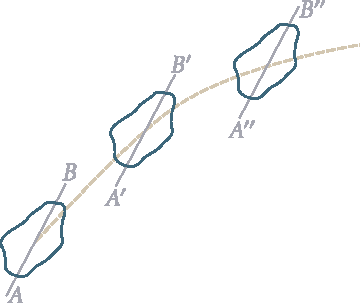
\includegraphics[scale=0.95]{figures/ch_01/fig_1_1.pdf}
			\caption[]{}
			\label{fig:1_1}
		\end{center}
	\end{minipage}
	\hfill{ }%\hspace{-0.1cm}
	\begin{minipage}[t]{0.5\linewidth}
		\begin{center}
			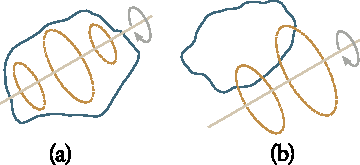
\includegraphics[scale=0.95]{figures/ch_01/fig_1_2.pdf}
			\caption[]{}
			\label{fig:1_2}
		\end{center}
	\end{minipage}
\end{figure}

Vì khi nói về một vật nào đó như về một chất điểm ta lãng quên quảng tính của nó nên khái niệm chuyển động quay quanh một trục xuyên qua nó là không áp dụng được cho vật đó.

Để có được khả năng mô tả chuyển động một cách định lượng, cần phải gắn với các vật tạo thành hệ quy chiếu một hệ tọa độ nào đó, chẳng hạn hệ tọa độ Descartes. Khi đó có thể sách định vị trí của chất điểm nếu cho ba số $x$, $y$, $z$ là các tọa độ Descartes của điểm này. Có thể thực hiện một hệ tọa độ, bằng việc chọn một mạng vuông góc gồm những thanh hoặc những thước tỷ lệ như nhau (\fig{1_3}). Tại các nút mạng này cần phải đặt các đồng hồ đồng bộ với nhau và giống hệt nhau. Vị trí của chất điểm và thời điểm ứng với nó được ghi theo các thang tỷ lệ và đồng hồ ở gần chất điểm nhất.

\begin{figure}[!htb]
	\begin{center}
		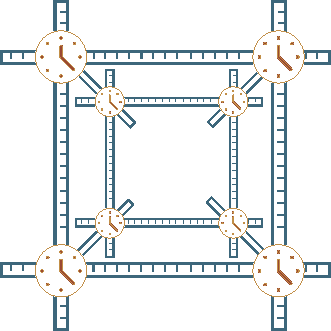
\includegraphics[scale=0.95]{figures/ch_01/fig_1_3.pdf}
		\caption[]{}
		\label{fig:1_3}
	\end{center}
\end{figure}

Đề cập tới một chất điểm, sẽ đơn giản hơn là đề cập tới một vật có kích thước dài. Do đó bước đầu chúng ta sẽ nghiên cứu cơ học của chất điểm, và sau đó ta sẽ chuyển qua cơ học của vật rắn. Ta bắt đầu trình bày từ động học, sau đó ta sẽ đi vào động lực học. Ta nhớ rằng \textbf{động học} nghiên cứu sự chuyển động của các vật mà không chú ý tới các nguyên nhân gây ra chuyển động này. \textbf{Động lực học} nghiên cứu chuyển động của các vật liên hệ với các nguyên nhân (với các tương tác giữa các vật) gây ra một tính chất nào đó của chuyển động.

\section{Một số kiến thức về vector}\label{sec:1_2}

\textbf{Định nghĩa vector.} Nguời ta gọi vector là một đại lượng được đặc trưng bằng trị số và hướng và ngoài ra có thể cộng theo quy tắc hình bình hành\footnote{Theo một định nghĩa chặt chẽ hơn, người ta gọi vector là một tập hợp ba đại lượng biến đổi theo một quy luật xác định khi quay các trục tọa độ.}. Yêu cầu sau cùng này là rất quan trọng. Có thể nêu ra các đại lượng mà chúng được đặc trưng bằng trị số và hướng, tuy nhiên được cộng khắc hẳn với các vector. Để làm ví dụ, ta hãy đưa ra sự quay của một vật quanh một trục nào đó một góc hữu hạn $\varphi$. Có thể biểu diễn sự quay như thế dưới dạng một đoạn thẳng có độ dài là $\varphi$, hướng theo trục mà phép quay được thực hiện xung quanh nó, về phía liên kết với chiều quay bằng quy tắc cái đinh ốc thuận. Trên \fig{1_4} ở dãy trên người ta đưa ra hai phép quay liên tiếp nhau của một quả cầu theo những góc $\pi/2$ được biểu diễn bằng các đoạn thẳng $\varphi_1$ và $\varphi_2$. Phép quay thứ nhất được thực hiện xung quanh trục $1$---$1$, dịch chuyển điểm  $A$ của quả cầu sang vị trí $A'$, được thực hiện xung quanh trục $2$---$2$, sang vị trí $A''$. Có thể đạt được cùng một kết quả như thế (tức là dịch chuyển điểm $A$ sang vị trí $A''$) bằng cách quay quả cầu xung quanh trục $3$---$3$ (xem dãy dưới ở \fig{1_4}) một góc $\pi$. Do đó cần phải coi phép quay đó như tổng của các phép quay $\varphi_1$ và $\varphi_2$. Tuy nhiên không thể có được nó từ những đoạn thẳng $\varphi_1$ và $\varphi_2$, bằng cách cộng chúng theo qui tắc hình bình hành. Một phép cộng như thế cho một đoạn thẳng có độ dài $\pi/\sqrt{2}$ thay cho độ dài $\pi$ cần phải có. Phép quay một góc $\pi/\sqrt{2}$ dịch chuyển điểm $A$ tới điểm $A'''$. Từ đó suy ra rằng các phép quay những góc hữu hạn được biểu diễn bằng những đoạn thẳng có hướng đều không có các tính chất của các vector.

\begin{figure}[!htb]
	\begin{center}
		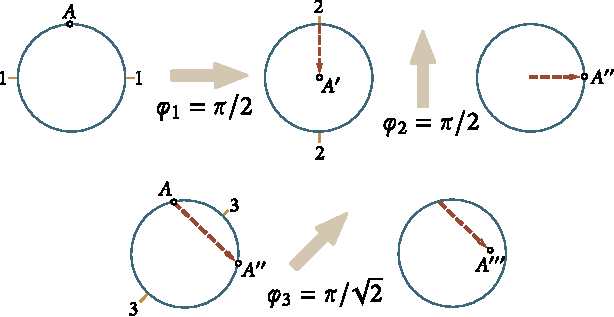
\includegraphics[scale=0.9]{figures/ch_01/fig_1_4.pdf}
		\caption[]{}
		\label{fig:1_4}
	\end{center}
\end{figure}

Trị số của vector được gọi là \textbf{module} của nó. Nói cách khác, module cho độ dài của vector. Module của vector là một vô hướng, do đó luôn luôn dương.

Trên các hình vẽ, các vector được biểu diễn dưới dạng các đoạn thẳng với mũi tên ở đầu. Độ dài của đoạn thẳng xác định module của vector trong tỷ lệ xích được thiết lập, còn mũi tên chỉ chiều của vector.

Người ta thường ký hiệu các vector bằng các chữ in đậm, chẳng hạn như $\vec{a}$, $\vec{b}$, $\vec{v}$ và $\vec{F}$. Cũng như thế nhưng in thường được dùng để ký hiệu module của vector $\vec{a}$\footnote{Trong khi viết, các vector được ký hiệu bằng các chữ với mũi tên ở trên chúng (chẳng hạn như $\oldvec{a}$). Trong trường hợp này, chính chữ đó mà không có mũi tên sẽ là module của vector.}. Đôi khi để ký hiệu module, đành phải dùng ký hiệu của vector đặt giữa hai vạch thẳng đứng: $|a|$ = module của vector $\vec{a}$. Cách ký hiệu như thế được sử dụng chẳng hạn cho module của tổng các vector $\vec{a}_1$ và $\vec{a}_2$:
\begin{equation}\label{eq:1_1}
	|\vec{a}_1 + \vec{a}_2| = \text{module của vector } (\vec{a}_1 + \vec{a}_2).
\end{equation}

\noindent
Trong trường hợp này ký hiệu $a_1+a_2$ có nghĩa là tổng các module của các vector số hạng, nói chung, không bằng module của tổng các vector (đẳng thức chỉ xảy ra trong trường hợp các vector có cùng hướng).

Các vector hướng dọc theo các đường thẳng song song cùng chiều hoặc ngược chiều nhau được gọi là các \textbf{vector đồng phương}. Các vector nằm trong các mặt phẳng song song được gọi là các \textbf{vector đồng phẳng}. Bằng sự dịch chuyển song song, các vector đồng phương có thể được đặt dọc theo cùng một đường thẳng, còn các vector đồng phẳng có thể được quy về một mặt phẳng.

Những vector đồng phương trùng nhau về module có cùng hướng được xem là bằng nhau\footnote{Lưu ý đến các \textbf{vector tự do}, nghĩa là các vector mà chúng có thể được đặt tại bất kỳ điểm nào trong không gian. Người ta cũng coi các \textbf{vector trượt} là các vector có gốc có thể được đặt tại bất kỳ điểm nào trên đường thẳng mà các vector được hướng dọc theo đó và các \textbf{vector buộc} nghĩa là các vector được đặt tại một điểm xác định. Hai dạng vector sau cùng này có thể được biểu thị qua các vector tự do: vì lý do này mà khái niệm vector tự do, thường được gọi đơn giản là vector, đã được đặt làm cơ sở cho phép tính vector.}

\textbf{Phép cộng và trừ các vector.} Để thuận tiện hơn, trong thực tế, khi cộng các vector người ta không vẽ hình bình hành. Như đã thấy trong \fig{1_5} người ta sẽ đạt được cùng một kết quả nếu đặt gốc của vector thứ hai trùng với ngọn của vector thứ nhất và sau đó vẽ vector tổng từ gốc của vector thứ nhất tới ngọn của vector thứ hai. Phương pháp như thế đặc biệt có lợi trong trường hợp khi phải cộng một số lượng vector lớn hơn hai (\fig{1_6}).

\begin{figure}[!htb]
	\begin{minipage}[t]{0.5\linewidth}
		\begin{center}
			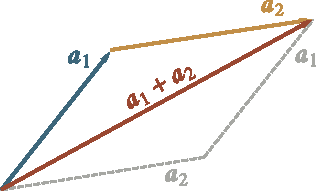
\includegraphics[scale=0.95]{figures/ch_01/fig_1_5.pdf}
			\caption[]{}
			\label{fig:1_5}
		\end{center}
	\end{minipage}
	\hfill{ }%\hspace{-0.1cm}
	\begin{minipage}[t]{0.5\linewidth}
		\begin{center}
			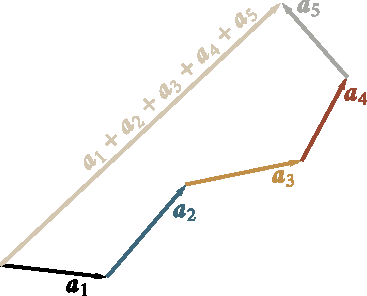
\includegraphics[scale=0.95]{figures/ch_01/fig_1_6.pdf}
			\caption[]{}
			\label{fig:1_6}
		\end{center}
	\end{minipage}
\end{figure}

Người ta gọi hiệu của hai vector $\vec{a}$ và $\vec{b}$ là một vector $\vec{c}$ mà khi cộng nó với $\vec{b}$ lại được vector $\vec{a}$ (\fig{1_7}---về vector $\vec{b}$ được biểu diễn bằng đường chấm chấm sẽ nói ở dưới). Chỉ có thể viết module của hai vector giống như module của tổng [xem \eqn{1_1}] bằng các vạch thẳng đứng:
\begin{equation}\label{eq:1_2}
|\vec{a}_1 - \vec{a}_2| = \text{module của vector } (\vec{a}_1 - \vec{a}_2),
\end{equation}

\noindent
vì ký hiệu $a_1-a_2$ là hiệu các module của các vector $\vec{a_1}$ và $\vec{a_2}$ mà nói chung không bằng không bằng module của hiệu.

\textbf{Phép nhân một vector với một vô hướng.} Kết quả nhân vector $\vec{a}$ với vô hướng $\alpha$ ta được vector mới $\vec{b}=\alpha$ có module lớn gấp $|\alpha|$ lần module của vector $\vec{a}$ ($b=|\alpha|a$). Chiều của vector $\vec{b}$ hoặc trùng với chiều của vector $\vec{a}$ (nếu $\alpha>0$), hoặc ngược với chiều của vector $\vec{a}$ (nếu $\alpha<0$). Từ điều đã nói trên suy ra rằng, phép nhân với $-1$ sẽ đổi ngược chiều của vector. Do đó các vector $\vec{a}$ và $-\vec{a}$ có các module như nhau nhưng ngược về chiều. Theo \fig{1_7} dễ dàng khẳng định rằng phép trừ vector $\vec{a}$ với vector $\vec{b}$ tương đương với việc thêm vector $\vec{-b}$ và vector $\vec{a}$.

Từ định nghĩa về phép toán nhân một vector với một vô hướng suy ra rằng mọi vector $\vec{a}$ có thể biểu diễn dưới dạng
\begin{equation}\label{eq:1_3}
\vec{a} = a\,\vecuni{a},
\end{equation}

\noindent
trong đó $a$ là module của vector $\vec{a}$, $\vecuni{a}$là vector có module bằng đơn vị và cùng chiều với vector $\vec{a}$ (\fig{1_8}).

Vector $\vecuni{a}$ được gọi là \textbf{vector đơn vị} hoặc là \textbf{chuẩn} của vector $\vec{a}$. Có thể biểu diễn chuẩn dưới dạng
\begin{equation}\label{eq:1_4}
\vecuni{a} = \frac{\vec{a}}{a},
\end{equation}

\noindent
từ đó suy ra rằng chuẩn là một đại lượng không có thứ nguyên.

\begin{figure}[!htb]
	\begin{minipage}[t]{0.5\linewidth}
		\begin{center}
			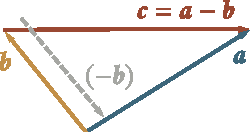
\includegraphics[scale=0.9]{figures/ch_01/fig_1_7.pdf}
			\caption[]{}
			\label{fig:1_7}
		\end{center}
	\end{minipage}
	\hfill{ }%\hspace{-0.1cm}
	\begin{minipage}[t]{0.5\linewidth}
		\begin{center}
			
\includegraphics[scale=0.95]{figures/ch_01/fig_1_8.pdf}
			\caption[]{}
			\label{fig:1_8}
		\end{center}
	\end{minipage}
\end{figure}

Có thể đưa ra các chuẩn không chỉ cho các vector mà cả cho các hướng bất kỳ trong không gian. Chẳng hạn như $\vecuni{x}$ là chuẩn của trục tọa độ $x$, $\vecuni{n}$ là chuẩn của pháp tuyến của đường hoặc mặt cong, and $\vecuni{\tau}$ là chuẩn của tiếp tuyến của đường cong.

\textbf{Sự phụ thuộc tuyến tính giữa các vector.} Ta hãy xét ba vector không đồng phương $\vec{a}$, $\vec{b}$ và $\vec{c}$ nằm trên một mặt phẳng. Từ \fig{1_9} rõ ràng là một vector bất kỳ trong chúng ($\vec{c}$ chẳng hạn) có thể được biểu diễn qua hai vector kia nhờ hệ thức
\begin{equation}\label{eq:1_5}
\vec{c} = \alpha\vec{a} + \beta\vec{b},
\end{equation}

\noindent
trong đó $\alpha$ và $\beta$ là các số nào đó (đối với trường hợp trình bày trên hình: $\alpha>1$, $-1<\beta<0$). Từ đó ta kết luận rằng vector $\vec{c}$ bất kỳ nằm trong một mặt phẳng với các vector không đồng phương, $\vec{a}$ và $\vec{b}$ có thể được biểu diễn qua các vector này nhờ hệ thức tuyến tính\eqref{eq:1_5}. Với các vector cố định $\vec{a}$ và $\vec{b}$ một vector thứ ba bất kỳ được xác định đơn trị bằng hai đại lượng $\alpha$ và $\beta$.

Giả sử cho ba vector $\vec{a}$, $\vec{b}$, $\vec{c}$ mà từng vector trong chúng không đồng phẳng với hai vector còn lại\footnote{Hai vector là luôn luôn đồng phẳng. Điều này suy ra từ chỗ là có thể làm trùng gốc của chúng bằng một sự dịch chuyển song song. Khi đó chúng được đặt trong một mặt phẳng.} Tương tự như \eqn{1_5} dễ dàng đoán ra rằng vector $\vec{d}$ bất kỳ có thể biểu diễn như một tổ hợp tuyến tính của các vector đã cho:
\begin{equation}\label{eq:1_6}
\vec{d} = \alpha\vec{a} + \beta\vec{b} + \gamma\vec{c},
\end{equation}

\noindent
Với các vector cố định $\vec{a}$, $\vec{b}$ và $\vec{c}$ vector $\vec{d}$ bất kỳ được xác định đơn trị bằng ba đại lượng $\alpha$, $\beta$ và $\gamma$, mà từng đại lượng có thể hoặc dương hoặc âm.

\textbf{Hình chiếu của một vector.} Ta xét một hướng nào đó trong không gian mà ta quy định là trục $l$ (\fig{1_10}). Giả thử vector $\vec{a}$ tạo với trục $l$ một góc $\varphi$ $l$\footnote{Nếu một đường thẳng mà vector $\vec{a}$ luôn hướng dọc theo đó và trục $l$ không cắt nhau thì để xác định góc $\varphi$ cần phải lấy một đường thẳng song song với vector $\vec{a}$ và cắt trục $l$. Góc giữa đường thẳng này và trục $l$ sẽ là góc $\varphi$ mà ta cần đến.}. Đại lượng
\begin{equation}\label{eq:1_7}
a_l = a\, \cos\varphi
\end{equation}

\noindent
($a$ là module của vector) được gọi là hình chiếu của vector $\vec{a}$ trên trục $l$.Hình chiếu được ký hiệu cùng một chữ như vector có thêm một chi số chỉ hướng mà vector được chiếu lên đó.

\begin{figure}[!htb]
	\begin{minipage}[htb!]{0.5\linewidth}
		\begin{center}
			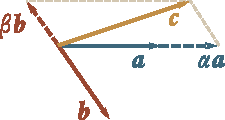
\includegraphics[scale=1]{figures/ch_01/fig_1_9.pdf}
			\caption[]{}
			\label{fig:1_9}
		\end{center}
	\end{minipage}
	\hfill{ }%\hspace{-0.1cm}
	\begin{minipage}[htb!]{0.5\linewidth}
		\begin{center}
			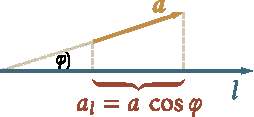
\includegraphics[scale=0.95]{figures/ch_01/fig_1_10.pdf}
			\caption[]{}
			\label{fig:1_10}
		\end{center}
	\end{minipage}
\end{figure}

Hình chiếu của vector là một đại lượng đại số. Nếu vector tạo với chiều đã cho một góc nhọn thì $\cos\varphi>0$, cho nên hình chiếu là dương. Nếu góc $\varphi$ là góc tù thì $\cos\varphi<0$ và do đó hình chiếu là âm. Khi vector vuông góc với trục đã cho thì hình chiếu bằng không. 

Hình chiếu của vector có một ý nghĩa hình học đơn giản. Nó bằng khoảng cách giữa các hình chiếu lên trục của gốc và ngọn của đoạn thẳng biểu diễn vector đã cho. Trong trường hợp $\varphi<\pi/2$ thì khoảng cách này lấy dâu cộng, trong trường hợp $\varphi>\pi/2$, nó lấy dấu trừ.

Giả thử $\vec{a} = \vec{a}_1+\vec{a}_2+\vec{a}_3+\vec{a}_4$ (\fig{1_11}). Từ hình vẽ dễ dàng kết luận rằng hình chiếu của vector tổng a lên một hướng nào đó bằng tổng hình chiếu của các vector số hạng:
\begin{equation}\label{eq:1_8}
a_l = a_{1l}+a_{2l}+a_{3l}+a_{4l}.
\end{equation}

\noindent
Ta hãy nhớ rằng, khi lấy tổng các hình chiếu của các vector biểu diễn trên \fig{1_11}, cần phải lấy các khoảng cách $0$---$1$, $1$---$2$, và $2$---$3$ với dấu cộng còn khoảng cách $3$---$4$ lấy dấu trừ. Công thức \eqref{eq:1_8} vẫn đúng với một số bất kỳ các số hạng.

\textbf{Biểu diễn vector qua các hình chiều của nó lên các trục tọa độ.} Ta hãy lấy các trục tọa độ Descartes và xét một vector $\vec{a}$ nằm trong mặt phẳng vuông góc với trục $z$ (\fig{1_12}). Ta hãy đưa vào các chuẩn của các trục tọa độ, tức là các vector đơn vị $\vecuni{x}$, $\vecuni{y}$, $\vecuni{z}$ ($\vecuni{z}$ không được vẽ trên hình, nó vuông góc với mặt phẳng của hình vẽ và hướng về phía chúng ta). Ta hãy chú ý rằng bộ ba chuẩn này hoàn toàn xác định hệ tọa độ và do đó được gọi là \textbf{cơ sở của hệ tọa độ}.

\begin{figure}[!htb]
	\begin{minipage}[t]{0.5\linewidth}
		\begin{center}
			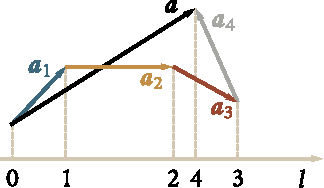
\includegraphics[scale=1]{figures/ch_01/fig_1_11.pdf}
			\caption[]{}
			\label{fig:1_11}
		\end{center}
	\end{minipage}
	\hfill{ }%\hspace{-0.1cm}
	\begin{minipage}[t]{0.5\linewidth}
		\begin{center}
			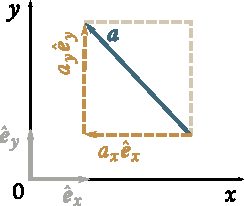
\includegraphics[scale=0.95]{figures/ch_01/fig_1_12.pdf}
			\caption[]{}
			\label{fig:1_12}
		\end{center}
	\end{minipage}
\end{figure}

Từ \fig{1_12} rõ ràng có thể biểu diễn vector $\vec{a}$ dưới dạng một tổ hợp tuyến tính chuẩn $\vecuni{x}$ và $\vecuni{y}$ [xem \eqn{1_5}]:
\begin{equation*}
\vec{a} = a_x \vecuni{x} + a_y \vecuni{y}.
\end{equation*}

\noindent
Các hình chiếu của vector lên các trục tọa độ đóng vai trò các hệ số $\alpha$ và $\beta$. Trong ví dụ được xét, hình chiếu $a_x$ là âm, do đó vector $a_x\vecuni{x}$ có chiều ngược lại với chiều của chuẩn $\vecuni{x}$.

Ta đã lấy vector $\vec{a}$ vuông góc với trục $z$, do đó vector $a_z=0$. Trong trường hợp tổng quát khi tất cả ba hình chiếu của vector đều khác không:
\begin{equation}\label{eq:1_9}
\vec{a} = a_x \vecuni{x} + a_y \vecuni{y} + a_z \vecuni{z},
\end{equation}

\noindent
Như vậy, có thể biểu diễn một vector bất kỳ quá các hình chiếu của nó lên các trục tọa độ được gọi là \textbf{các thhành phần} của vector.

Các đại lượng $a_x$, $a_y$, $a_z$ bằng (chính xác đến dấu) các cạnh của một hình hộp chữ nhật mà đường chéo lơn của nó là vector $\vec{a}$ (\fig{1_13}). Do đó có hệ thức
\begin{equation}\label{eq:1_10}
a^2 = a_x^2 + a_y^2 + a_z^2.
\end{equation}

Giả thử $\vec{c}=\vec{a}+\vec{b}$. Biểu diễn từng vector theo đúng công thức \eqn{1_9}, ta có
\begin{equation*}
c_x\vecuni{x} + c_y\vecuni{y} + a_z\vecuni{z} = (a_x+b_x)\vecuni{x} + (a_y+b_y)\vecuni{y} + (a_z+b_z)\vecuni{z}
\end{equation*}

\noindent
(ta đưa ra ngoài các dấu ngoặc các thừa số chung $\vecuni{x}$, $\vecuni{y}$ và $\vecuni{z}$)· Các vector bằng nhau đều có các hình chiếu bằng nhau trên các trục tọa độ. Trên cơ sở này có thể viết là
\begin{equation}\label{eq:1_11}
c_x=a_x+b_x,\quad c_y=a_y+b_y,\quad a_z=a_z+b_z
\end{equation}

\noindent
[so sánh với \eqn{1_8}]. Các công thức \eqref{eq:1_11} là biểu thúc giải tích của qui tắc cộng các vector. Chúng đúng với một số bất kỳ các số hạng

\textbf{Bán kính vector.} Người ta gọi bán kính vector $\vec{r}$ của một điểm nào đó là một vector vẽ từ gốc tọa độ tới điểm đã cho (\fig{1_14}). Các hình chiếu của nó lên các trục tọa độ đều bằng các tọa độ Descartes của điểm đã cho:
\begin{equation}\label{eq:1_12}
r_x=x,\quad r_y=y,\quad r_z=z.
\end{equation}

\noindent
Do đó, ứng với \eqn{1_9} có thể biểu diễn bán kính vector dưới dạng
\begin{equation}\label{eq:1_13}
\vec{r} = x\vecuni{x} + y\vecuni{y} + z\vecuni{z}.
\end{equation}

\noindent
Theo \eqn{1_10}
\begin{equation}\label{eq:1_14}
r^2 = x^2 + y^2 + z^2.
\end{equation}

\begin{figure}[!htb]
	\begin{minipage}[t]{0.5\linewidth}
		\begin{center}
			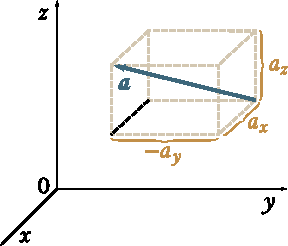
\includegraphics[scale=1]{figures/ch_01/fig_1_13.pdf}
			\caption[]{}
			\label{fig:1_13}
		\end{center}
	\end{minipage}
	\hfill{ }%\hspace{-0.1cm}
	\begin{minipage}[t]{0.5\linewidth}
		\begin{center}
			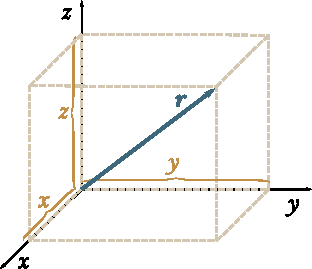
\includegraphics[scale=0.95]{figures/ch_01/fig_1_14.pdf}
			\caption[]{}
			\label{fig:1_14}
		\end{center}
	\end{minipage}
\end{figure}

\textbf{Tích vô hướng của các vector.} Có thể nhân hai vector $\vec{a}$ và $\vec{b}$ với nhau theo hai cách, một cách dẫn tới đại lượng vô hướng, cách kia cho kết quả là một vector mới nào đó. Ứng với điều này có hai tích của các vector---tích vô hướng và tích vector. Ta hãy chú ý rằng \textit{không có phép tính chia một vector cho một vector}.

Người ta gọi tích vô hướng của các vector $\vec{a}$ và $\vec{b}$ là một vô hướng bằng tích các module của các vector này với cos của góc $\alpha$ giữa chúng:
\begin{equation}\label{eq:1_15}
\vecdot{a}{b} = ab\cos\alpha
\end{equation}

\noindent
(\fig{1_15}). When writing a scalar product, the symbols of the vectors being multiplied are usually written next to each other with dot between them (this is why a scalar product is also called a dot product; sometimes nothing is used between the symbols)\footnote{The dot symbol between vectors is preferred in the \LaTeX version to adopt a more modern approach.}. Equation~\eqref{eq:1_15} expresses an algebraic quantity: when $\alpha$ is acute, we have $\vecdot{a}{b}>0$, and when it is obtuse, we have $\vecdot{a}{b}<0$. The scalar product of mutually perpendicular vectors ($\alpha=\pi/2$) equals zero.

\begin{figure}[!htb]
	\begin{center}
		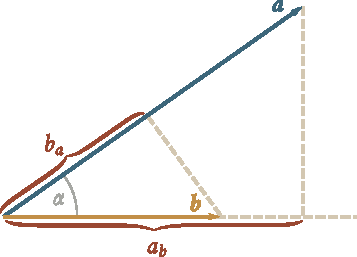
\includegraphics[scale=0.9]{figures/ch_01/fig_1_15.pdf}
		\caption[]{}
		\label{fig:1_15}
	\end{center}
\end{figure}

Ta hãy chú ý rằng bình phương của một vector luôn luôn được hiểu ngầm là tích vô hướng của vector với chính nó:
\begin{equation}\label{eq:1_16}
\vec{a}^2 = \vecdot{a}{a} = aa\cos\alpha = a^2.
\end{equation}

\noindent
Như vậy bình phương của một vector bằng bình phương module của nó. Đặc biệt là bình phương của một chuẩn bất kỳ bằng đơn vị:
\begin{equation}\label{eq:1_17}
\vecuni{x}^2 = \vecuni{y}^2 = \vecuni{z}^2 = 1.
\end{equation}

\noindent
Đồng thời ta hãy chú ý rằng do các chuẩn vuông góc với nhau nên các tích vô hướng có dạng $\vecunidot{i}{k}$ đều bằng không, nếu $i\neq k$.

Dùng ký hiệu Kronecker $\delta_{ik}$ được định nghĩa như sau:
\begin{equation}\label{eq:1_18}
\delta_{ik} = \begin{cases}
1, &\mbox{if } i = k, \\
0, &\mbox{if } i\neq k. \end{cases}
\end{equation}
là rất tiện lợi.

\noindent
Nếu sử dụng ký hiệu này thì có thể biểu thị các tính chất đã thiết lập ở trên của các tích vô hướng các chuẩn của các trục tọa độ bằng một công thức:
\begin{equation}\label{eq:1_19}
\vecunidot{i}{k} = \delta_{ik}\quad (i, k = x, y, z)
\end{equation}

\noindent
(các chỉ số $i$ và $k$ có thể lấy các giá trị $x$, $y$ và $z$ độc lập với nhau).

Từ định nghĩa \eqref{eq:1_15} suy ra rằng, tích vô hướng có tính giao hoán, nghĩa là không phụ thuộc vào thứ tự các nhân tử:
\vspace{-12pt}
\begin{equation}\label{eq:1_20}
\vecdot{a}{b} = \vecdot{b}{a}.
\end{equation}

\noindent
Có thể viết biểu thức \eqref{eq:1_15} theo một số cách:
\begin{equation*}
\vecdot{a}{b} = ab\cos\alpha = (a\cos\alpha)\,b = a\,(b\cos\alpha).
\end{equation*}

\noindent
Từ \fig{1_15} rõ ràng là $a\cos\alpha$ bằng $a_b$ là hình chiếu của vector $\vec{a}$ lên hướng của vector $\vec{b}$. Một cách tương tự, $b\cos\alpha= b_a$ là hình chiếu của vector $\vec{b}$ lên hướng của vector $\vec{a}$. Do đó có thể nói rằng, người ta gọi tích vô hướng của hai vector là một vô hướng bằng tích module của một vector nhân tử với hình chiếu của vector kia lên hướng của vector này:
\begin{equation}\label{eq:1_21}
\vecdot{a}{b} = a_b b = a b_a.
\end{equation}

Nếu để ý rằng hình chiếu của tổng các vector bằng tổng các hình chiếu của các vector số hạng thì ta có thể viết:
\begin{equation}\label{eq:1_22}
\vec{a}\boldsymbol{\cdot}(\vec{b}+\vec{c}+\ldots) = a(\vec{b}+\vec{c}+\ldots)_a = a(b_a+c_a+\ldots) = ab_a+ac_a+\ldots = ab+ac+\ldots .
\end{equation}

\noindent
Từ đó suy ra rằng tích vô hướng của các vector có tính phân phối, nghĩa là tích của vector $\vec{a}$ với tổng một số vector bằng tổng các tích của vector $\vec{a}$ với mỗi vector số hạng được lấy tách biệt.

Biểu diễn các vector nhân tử dưới dạng \eqn{1_9} và sử dụng tính phân phối của tích vô hướng, ta có:
\begin{align*}
\vecdot{a}{b} &= (a_x\vecuni{x} + a_y\vecuni{y} + a_z\vecuni{z})(b_x\vecuni{x} + b_y\vecuni{y} + b_z\vecuni{z})\\
&= a_xb_x\vecunidot{x}{x} + a_xb_y\vecunidot{x}{y} + a_xb_z\vecunidot{x}{z} + a_yb_x\vecunidot{y}{x} + a_yb_y\vecunidot{y}{y}\\
&\,+ a_yb_z\vecunidot{y}{z}+ a_zb_x\vecunidot{z}{x} + a_zb_y\vecunidot{z}{y} + a_zb_z\vecunidot{z}{z}.
\end{align*}

\noindent
Bây giờ hãy chú ý đến \eqn{1_19}. Kết quả là ta được biểu thức của tích vô hướng qua các hình chiếu của các vector nhân tử:
\begin{equation}\label{eq:1_23}
\vecdot{a}{b} = a_xb_x + a_yb_x + a_zb_z.
\end{equation}

\noindent
Ta chú ý rằng khi quay các trục tọa độ thì các hình chiếu của các vector trên các trục này sẽ bị biến đổi. Tuy nhiên đại lượng $ab\cos\alpha$ không phụ thuộc vào việc chọn trục. Từ đó ta kết luận rằng các biến đổi hình chiếu của các vector $\vec{a}$ và $\vec{b}$ khi quay các trục mang một đặc tính là tổ hợp của chúng có dạng \eqn{1_23} vẫn bất biến (không biến đổi):
\begin{equation}\label{eq:1_24}
\vecdot{a}{b} = a_xb_x + a_yb_x + a_zb_z = \mathrm{inv}.
\end{equation}

Dễ dàng hiểu được rằng có thể biểu diễn hình chiếu của vector $\vec{a}$ lên hướng $l$ [xem \eqn{1_7}] dưới dạng
\begin{equation}\label{eq:1_25}
a_l = \vec{a}\boldsymbol{\cdot}\vecuni{l},
\end{equation}

\noindent
trong đó $\vecuni{l}$ là chuẩn của hướng $l$. Một cách tương tự,
\begin{equation}\label{eq:1_26}
a_x = \vec{a}\boldsymbol{\cdot}\vecuni{x},\quad  a_y = \vec{a}\boldsymbol{\cdot}\vecuni{y}, \quad  a_z=\vec{a}\boldsymbol{\cdot}\vecuni{z}.
\end{equation}

\textbf{Tích vector.} Người ta gọi vector $\vec{c}$ được xác định bằng công thức
\begin{equation}\label{eq:1_27}
\vec{c} = ab\sin(\alpha)\hatvec{n},
\end{equation}
là tích vector của các vector $\vec{a}$ và $\vec{b}$.

\noindent
Trong đó $a$ và $b$ là các module của các vector nhân tử, $\alpha$ là góc ở giữa các vector, $\hatvec{n}$ là vector đơn vị của pháp tuyến\footnote{Ký hiệu $\hatvec{n}$ đơn giản hơn và trực quan hơn là $\vecuni{n}$.} với mặt phẳng chứa các vector $\vec{a}$ và $\vec{b}$ (\fig{1_16}).

Chiều của $\hatvec{n}$ được chọn sao cho dãy các vector $\vec{a}$, $\vec{b}$, $\hatvec{n}$ tạo thành một hệ đinh ốc thuận. Điều này có nghĩa là nếu nhìn theo vector $\hatvec{n}$ thì phép quay theo con đường ngắn nhất từ nhân tử thứ nhất tới nhân tử thứ hai được thực hiện theo chiều quay của kim đồng hồ. Trên \fig{1_16}, vector $\hatvec{n}$ hướng ra sau hình vẽ và do đó được biểu diễn bằng một vòng tròn nhỏ có dấu chữ thập\footnote{Chúng ta sẽ biểu diễn các vector vuông góc với mặt phẳng hình vẽ bằng một vòng tròn nhỏ có dấu chữ thập nếu vector hướng ra xa ta, và bằng một vòng tròn nhỏ có điểm chấm ở tâm nếu vector hướng về ta. Để dễ thấy, có thể hình dung một vector dưới dạng một mũi tên với phần đầu có dạng hình nón và phần đuôi có dạng hình chữ thập. Khi đó nếu vector hướng về phía chúng ta (mũi tên bay tới chúng ta), ta sẽ nhìn thấy một vòng tròn nhỏ với điểm chấm, nếu cũng vector đó hướng ra xa chúng ta (mũi tên bay ra xa ta), ta sẽ nhìn thấy một vòng tròn với dấu chữ thập.}. Hướng của vector $\vec{c}$ trùng với hướng của $\hatvec{n}$.

\begin{figure}[!htb]
	\begin{center}
		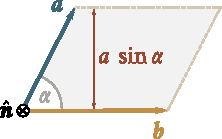
\includegraphics[scale=1]{figures/ch_01/fig_1_16.pdf}
		\caption[]{}
		\label{fig:1_16}
	\end{center}
\end{figure}

Có thể viết một cách tượng trưng tích vector theo hai cách:
\begin{equation*}
[\vec{a},\vec{b}]\quad\text{hoặc}\quad \vec{a}\times\vec{b}
\end{equation*}

\noindent
the latter notation resulting in the term cross product sometimes being used to signify a vector product. We shall use the latter notation\footnote{To avoid confusion, in the \LaTeX version, we shall use the cross product symbol.}. Thus, according to \eqn{1_27}, we have
\begin{equation}\label{eq:1_28}
\vecprod{a}{b} = (ab\sin\alpha)\hatvec{n}.
\end{equation}

Từ \fig{1_16} rõ ràng là module của vector tích có ý nghĩa hình học đơn giản---biểu thức $ab\sin\alpha$ về trị số bằng điện tích hình bình hành tạo bởi các vector nhân tử.

Chúng ta đã xác định hướng của vector $\vecprod{a}{b}$ bằng cách liên kết nó với chiều quay từ nhân tử thứ nhất tới nhân tử thứ hai. Khi khảo sát các vector như bán kính vector $\vec{r}$, vận tốc $\vec{v}$, lực $\vec{F}$,...vấn đề chọn hướng của chúng không đặt ra vì nó suy ra một cách tự nhiên từ bản chất của chính các đại lượng. Các vector như thế được gọi là các \textbf{vector thực} (hoặc các vector cực). Các vector loại $\vecprod{a}{b}$ có chiều liên kết với chiều quay được gọi là \textbf{giả vector} (hoặc các vector trục). Khi thay đổi điều kiện, chẳng hạn khi chuyển từ hệ tọa độ thuận sang hệ tọa độ nghịch, chiều của các giả vector biến đổi ngược lại, trong lúc đó các vector thực vẫn không biến đổi.

Cần chú ý rằng tích vector sẽ là một giả vector chỉ trong trường hợp khi cả hai vector nhân tử đều là các vector thực (hoặc cả hai đều là các giả vector). Tích vector của một vector thực với một giả vector sẽ là một vector thực. Sự thay đổi ngược lại điều kiện xác định chiều của các giả vector trong trường hợp này dẫn tới sự đổi dấu đứng trước tích vector và đồng thời dẫn tới sự đổi dấu đứng trước một trong các nhân tử. Rốt cuộc là đại lượng được biểu thị bằng tích vector vẫn không đổi.

Vì chiều của tích vector được xác định bằng chiều quay từ nhân tử thú nhất tới nhân tử thứ hai nên kết quả của phép nhân vector phụ thuộc vào thứ tự của các nhân tử. Sự hoán vị các nhân tử gây ra sự đổi ngược lại chiều của vector kết quả. Như vậy, tích vector không có tính chất giao hoán:
\begin{equation}\label{eq:1_29}
\vecprod{a}{b} = -\vecprod{b}{a}.
\end{equation}

\noindent
Có thể chứng minh rằng tích vector có tính phân phối, nghĩa là
\begin{equation}\label{eq:1_30}
\vec{a}\times(\vec{b}_1+\vec{b}_2+\ldots)] = \vec{a}\times\vec{b}_1 + \vec{a}\times\vec{b}_2 + \ldots.
\end{equation}

\begin{figure}[!htb]
	\begin{center}
		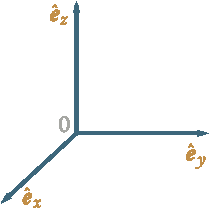
\includegraphics[scale=1]{figures/ch_01/fig_1_17.pdf}
		\caption[]{}
		\label{fig:1_17}
	\end{center}
\end{figure}

Ta hãy xét các tích vector của các chuẩn của các trục tọa độ (\fig{1_17}). Theo định nghĩa \eqref{eq:1_28}
\begin{align}
\vecuniprod{x}{x} &= \vecuniprod{y}{y} = \vecuniprod{z}{z} = 0,\nonumber\\
\vecuniprod{x}{y} &= -\vecuniprod{y}{x} = \vecuni{z},\label{eq:1_31}\\
\vecuniprod{y}{z} &= -\vecuniprod{z}{y} = \vecuni{x},\nonumber\\
\vecuniprod{z}{x} &= -\vecuniprod{x}{z} = \vecuni{y}.\nonumber
\end{align}

\noindent
Biểu diễn các vector dưới dạng \eqn{1_9} và sử dụng tính phân phối của tích vector ta có:
\begin{align*}
\vecprod{a}{b} &= (a_x\vecuni{x}+a_y\vecuni{y}+a_z\vecuni{z})\times(b_x\vecuni{x}+b_y\vecuni{y}+b_z\vecuni{z})\\
&= a_xb_x\vecuniprod{x}{x} + a_xb_y\vecuniprod{x}{y} + a_xb_z\vecuniprod{x}{z}\\
&+ a_yb_x\vecuniprod{y}{x} + a_yb_y\vecuniprod{y}{y} + a_yb_z\vecuniprod{y}{z}\\
&+ a_zb_x\vecuniprod{z}{x} + a_zb_y\vecuniprod{z}{y} + a_zb_z\vecuniprod{z}{z}
\end{align*}

\noindent
Nếu chú ý đến hệ thức \eqref{eq:1_31}, ta đi tới biểu thức sau:
\begin{equation}\label{eq:1_32}
\vecprod{a}{b} = \vecuni{x}(a_yb_z - a_zb_y) + \vecuni{y}(a_zb_x - a_xb_z) + \vecuni{z}(a_xb_y - a_yb_x).
\end{equation}

\noindent
Có thể biểu diễn biểu thức thu được dưới dạng định thức:
\vspace{-12pt}
\begin{equation}\label{eq:1_33}
\vecprod{a}{b} = \begin{vmatrix}
\vecuni{x} & \vecuni{y} & \vecuni{z}\\
a_x & a_y & a_z\\
b_x & b_y & b_z
\end{vmatrix}.
\end{equation}

\textbf{Tích hỗn hợp.} Biểu thức $\vecmix{a}{b}{c}$ được gọi là tích hỗn hợp (hoặc tích vô hướng-vector) của ba vector, nghĩa là tích vô hướng của vector $\vec{a}$ với tích vector của các vector $\vec{b}$ và $\vec{c}$. Theo các định nghĩa \eqref{eq:1_15} và \eqref{eq:1_28}
\begin{equation*}
\vecmix{a}{b}{c} = a\{bc\sin(\vec{b}, \vec{c})\}\cos(\vec{a},\hatvec{n}).
\end{equation*}

\begin{figure}[!htb]
	\begin{center}
		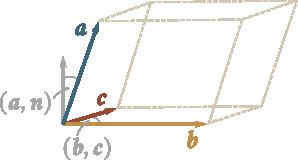
\includegraphics[scale=1]{figures/ch_01/fig_1_18.pdf}
		\caption[]{}
		\label{fig:1_18}
	\end{center}
\end{figure}

\noindent
Ở đây $(\vec{b},\vec{c})$ là góc giữa $\vec{b}$ và $\vec{c}$, $(\vec{a},\hatvec{n})$ là góc giữa vector $\vec{a}$ và chuẩn $\hatvec{n}$ xác định $\vecprod{b}{c}$. Từ \fig{1_18} rõ ràng là biểu thức $bc\sin(\vec{b},\vec{c})$ về trị số bằng diện tích đáy của hình hộp được tạo bởi các vector nhân tử còn biểu thức $a\cos(\vec{a},\hatvec{n})$ về trị số bằng chiều cao của hình hộp này lấy với dấu cộng nếu góc $(\vec{a},\hatvec{n})$ là nhọn và với dấu trừ nếu góc này là tù. Do đó biểu thức $\vecmix{a}{b}{c}$ có ý nghĩa hình học đơn giản---về trị số nó bằng thể tích của hình hộp được tạo bởi các vector nhân tử [lấy dấu cộng hay trừ tùy theo độ lớn của góc $(\vec{a},\hatvec{n})$]. Khi tính thể tích của hình hộp, kết quả không thể phụ thuộc vào điều là mặt nào trong các mặt của nó được lấy làm đáy. Từ đó suy ra rằng
\begin{equation}\label{eq:1_34}
\vecmix{a}{b}{c} = \vecmix{b}{c}{a} = \vecmix{c}{a}{b}.
\end{equation}

\noindent
Như vậy, tích hỗn hợp cho phép hoán vị vòng quanh các nhân tử, nghĩa là cho phép thay thế mỗi nhân tử tiếp sau đó theo chu trình:
\begin{equation*}
% \begin{tikzcd}
% \vec{a}\arrow[rd] &\\
% \vec{c}\arrow[u] & \arrow[l] \vec{b}
% \end{tikzcd}
\begin{tikzcd}[column sep=small]
             & \vec{a} \arrow[rd] &              \\
\vec{c} \arrow[ru] &              & \vec{b} \arrow[ll]
\end{tikzcd}
\end{equation*}

\textbf{Tích vector kép.} Ta hãy nghiên cứu tích vector kép của vector $\vec{a}$, $\vec{b}$ và $\vec{c}$
\begin{equation*}
\vec{d} = \vec{a}\times\vecprod{b}{c}.
\end{equation*}

\noindent
Mỗi tích vector là vuông góc với cả hai nhân tử. Do đó vector $\vec{d}$ vuông góc với chuẩn $\hatvec{n}$ xác định hướng của vector $\vecprod{b}{c}$. Từ đó suy ra rằng vector $\vec{d}$ nằm trong mặt phẳng tạo bởi các vector $\vec{b}$ và $\vec{c}$, và do đó có thể được biểu diễn như một tổ hợp tuyến tính của các vector này:
\begin{equation*}
\vec{d} = \alpha\vec{b} + \beta\vec{c}
\end{equation*}

\noindent
[xem \eqn{1_5}]. Phép tính toán tương ứng cho $\alpha=\vecdot{a}{c}$, $\beta=-\vecdot{a}{b}$. Như vậy
\begin{equation}\label{eq:1_35}
\vec{a}\times\vecprod{b}{c} = \vec{b}(\vecdot{a}{c}) - \vec{c}(\vecdot{a}{b}).
\end{equation}

\textbf{Đạo hàm của vector.} Ta hãy nghiên cứu một vector biến đổi theo thời gian theo một quy luật đã biết $\vec{a}(t)$. Hình chiếu của vector này trên các trục tọa độ là các hàm độ cho của thời gian. Do đó
\begin{equation}\label{eq:1_36}
\vec{a}(t) = \vecuni{x}a_x(t) + \vecuni{y}a_y(t) + \vecuni{z}a_z(t)
\end{equation}

\noindent
(ta giả thiết rằng các thục tọa độ không quay trong không gian, cho nên các chuẩn của các trục không biến đổi theo thời gian).

Giả thử trong khoảng thời gian $\Delta t$, các hình chiếu của vector nhận các số gia $\Delta a_x$, $\Delta a_y$, $\Delta a_z$. Khi đó vector nhận số gia $\Delta\vec{a} = \vecuni{x}\Delta a_x + \vecuni{y}\Delta a_y + \vecuni{z}\Delta a_z$. Có thể đặc trưng vận tốc biển đổi của vector $\vec{a}$ theo giời gian bằng tỷ số giữa $\Delta\vec{a}$ và $\Delta t$:
\begin{equation}\label{eq:1_37}
\frac{\Delta\vec{a}}{\Delta t} = \vecuni{x}\frac{\Delta a_x}{\Delta t} + \vecuni{y}\frac{\Delta a_y}{\Delta t} + \vecuni{z}\frac{\Delta a_z}{\Delta t}.
\end{equation}

\noindent
Tỷ số này cho vận tốc biển đổi trung bình của $\vec{a}$ trong khoảng thời gian $\Delta t$. Ta hãy giả thử rằng $\vec{a}$ biến đổi theo thời gian một cách liên tục mà không có các đột biến. Khi đó khoảng thời gian $\Delta t$ càng nhỏ thì đại lượng \eqn{1_37} càng đặc trưng chính xác hơn cho vận tốc biến đổi của $\vec{a}$ tại thời điểm $t$ xảy ra trước khoảng $\Delta t$. Do đó vận tốc biến đổi của vector $\vec{a}$ tại thời điểm $t$ bằng giới hạn của tỷ số \eqn{1_37} có được khi giảm vô hạn $\Delta t$:
\begin{align}
\text{vận tốc biến đổi của }\vec{a} &= \lim_{\Delta t\to 0}\frac{\Delta\vec{a}}{\Delta t} \nonumber\\
&= \vecuni{x} \lim_{\Delta t\to 0}\frac{\Delta a_x}{\Delta t} + \lim_{\Delta t\to 0}\vecuni{y} \frac{\Delta a_y}{\Delta t} + \lim_{\Delta t\to 0}\vecuni{z} \frac{\Delta a_z}{\Delta t}.\label{eq:1_38}
\end{align}

Nếu có một hàm $f(t)$ nào đó của đối số $t$, thì giới hạn của tỷ số giữa số gia của hàm $\Delta f$ với số gia của đối số $\Delta t$ có được khi $\Delta t$ dần tới không được gọi là đạo hàm của hàm $f$ theo $t$ và được ký hiệu bằng ký hiệu $\diffin{f}{t}$. Do đó có thể viết biểu thức \eqref{eq:1_38} như sau:
\begin{equation}\label{eq:1_39}
\diff{\vec{a}}{t} = \vecuni{x}\diff{a_x}{t} + \vecuni{y}\diff{a_y}{t} + \vecuni{z}\diff{a_z}{t}.
\end{equation}

\noindent
Kết quả thu được có nghĩa là các hình chiếu của vector $\diffin{\vec{a}}{t}$ lên các trục tọa độ bằng đạo hàm theo thời gian của các vector $\vec{a}$:
\begin{equation}\label{eq:1_40}
\left(\diff{\vec{a}}{t}\right)_{\text{pr. }x} = \diff{a_x}{t},\quad \left(\diff{\vec{a}}{t}\right)_{\text{pr. }y} = \diff{a_y}{t},\quad \left(\diff{\vec{a}}{t}\right)_{\text{pr. }z} = \diff{a_z}{t},\quad.
\end{equation}

Trong vật lý người ta thường ký hiệu các đạo hàm theo thời gian bằng ký hiệu của đại lượng tương ứng với một dấu chấm ở trên nó, chẳng hạn
\begin{equation}\label{eq:1_41}
\diff{\varphi}{t} = \dot{\varphi},\quad \diffsec{\varphi}{t} = \ddot{\varphi},\quad \diff{\vec{a}}{t} = \dot{\vec{a}},\quad \diffsec{\vec{a}}{t} = \ddot{\vec{a}}.
\end{equation}

\noindent
Nếu sử dụng ký hiệu đó thì công thức \eqref{eq:1_39} có thể nhận dạng
\begin{equation}\label{eq:1_42}
\dot{\vec{a}} = \vecuni{x}\dot{a}_x + \vecuni{y}\dot{a}_y + \vecuni{z}\dot{a}_z.
\end{equation}

\noindent
Nếu lấy bán kính vector $\vec{r}(t)$ của điểm chuyển động để làm $\vec{a}(t)$ thì theo \eqn{1_42}
\begin{equation}\label{eq:1_43}
\dot{\vec{r}} = \vecuni{x}\dot{r}_x + \vecuni{y}\dot{r}_y + \vecuni{z}\dot{r}_z,
\end{equation}

\noindent
trong đó $x$, $y$, $z$ là các hàm của $x=x(t)$, $y=t(t)$, $z=z(t)$.

Biểu thức
\begin{equation}\label{eq:1_44}
\mathrm{d}f = f'\, \mathrm{d}t,
\end{equation}
được gọi là vi phân (``số gia'') của hàm $f(t)$.

\noindent
Trong đó $f'$ là đạo hàm của $f$ theo $t$.  Theo \eqn{1_39} vi phân (``số gia'') của vector $\vec{a}$ được xác định bằng công thức
\begin{equation}\label{eq:1_45}
\mathrm{d}\vec{a} = \vecuni{x}\mathrm{d}a_x + \vecuni{y}\mathrm{d}a_y + \vecuni{z}\mathrm{d}a_z.
\end{equation}

Đặc biệt là
\begin{equation}\label{eq:1_46}
\mathrm{d}\vec{r} = \vecuni{x}\mathrm{d}x + \vecuni{y}\mathrm{d}y + \vecuni{z}\mathrm{d}z.
\end{equation}

Ta hãy chú ý rằng trong một khoảng thời gian $\Delta t$ rất nhỏ nhưng hữu hạn, số gia của hàm xấp xỉ bằng
\begin{equation}\label{eq:1_47}
\Delta f \approx f'\Delta t = \diff{f}{t}\Delta t.
\end{equation}

\noindent
Tại giới hạn khi $\Delta t\to 0$, đằng thức gần đúng \eqref{eq:1_47} chuyển thành đẳng thức đúng \eqref{eq:1_44}.

Có thể viết công thức tương tự \eqref{eq:1_47} cả đối với hàm vector
\begin{equation}\label{eq:1_48}
\Delta\vec{a} \approx \diff{\vec{a}}{t}\Delta t.
\end{equation}

\textbf{Đạo hàm của tích các hàm.} Ta hãy nghiên cứu hàm $\vec{b}(t)$, nó bằng tích của hàm vô hướng $\varphi(t)$ và hàm vector $\vec{a}(t)$, $\vec{b}(t)=\varphi(t)\vec{a}(t)$, hoặc một cách ngắn gọn $\vec{b}=\varphi\vec{a}$. Ta hãy tìm số gia của hàm $\vec{b}$:
\begin{equation*}
\Delta\vec{b} = \Delta(\varphi\vec{a}) = (\varphi + \Delta\varphi)(\vec{a} + \Delta\vec{a}) - \varphi\vec{a} = \varphi\Delta\vec{a} + \vec{a}\Delta\varphi + \Delta\varphi\Delta\vec{a}.
\end{equation*}

\noindent
Nếu biêu diễn số gia của hàm dưới dạng \eqref{eq:1_47} và \eqref{eq:1_48}, ta có:
\begin{equation*}
\Delta\vec{b} \approx \varphi\diff{\vec{a}}{t}\Delta t + \vec{a}\diff{\varphi}{t}\Delta t + \diff{\varphi}{t}\diff{\vec{a}}{t}(\Delta t)^2
\end{equation*}

\noindent
từ đó
\begin{equation*}
\frac{\Delta\vec{b}}{\Delta t} \approx \varphi\diff{\vec{a}}{t} + \vec{a}\diff{\varphi}{t} + \diff{\varphi}{t}\diff{\vec{a}}{t}\Delta t.
\end{equation*}

\noindent
Tại giới hạn khi $\mathrm{d}t$ tiến tới không, đẳng thức gần đúng này trở thành đẳng thức chính xác. Như vậy
\begin{equation*}
\diff{\vec{b}}{t} = \lim_{\Delta t\to 0} \diff{\vec{b}}{t} =  \lim_{\Delta t\to 0} \left(\varphi\diff{\vec{a}}{t} + \vec{a}\diff{\varphi}{t} + \diff{\varphi}{t} \diff{\vec{a}}{t}\Delta t\right).
\end{equation*}

\noindent
Hai số hạng đầu không phụ thuộc vào $\Delta t$ và do đó khi chuyển tới giới hạn sẽ không bị biến đổi. Giới hạn của số hạng thứ ba bằng không. Do đó, sau khi thay $\vec{b}$ bằng $\varphi\vec{a}$, ta có:
\begin{equation}\label{eq:1_49}
\diff{(\varphi\vec{a})}{t} = \varphi\diff{\vec{a}}{t} + \vec{a}\diff{\varphi}{t} = \varphi\dot{\vec{a}}+\dot{\varphi}\vec{a}.
\end{equation}

Bây giờ ta hãy nghiên cứu đạo hàm của tích vô hướng của hai hàm vector $\vec{a}(t)$ và $\vec{b}(t)$. Số gia của tích này bằng:
\begin{align*}
\Delta(\vec{a}\vec{b}) &= (\vec{a} + \Delta\vec{a})(\vec{b} + \Delta\vec{b}) - \vec{a}\vec{b}\\
&= \vec{a}\Delta\vec{b} + \vec{b}\Delta\vec{a} + \Delta\vec{a}\Delta\vec{b} \\
&\approx \vec{a}\dot{\vec{b}}\Delta t + \vec{b}\dot{\vec{a}}\Delta t + \dot{\vec{a}}\dot{\vec{b}}(\Delta t)^2
\end{align*}

\noindent
Từ đó
\begin{equation*}
\diff{(\vec{a}\vec{b})}{t} = \lim_{\Delta t\to 0} \frac{\Delta(\vec{a}\vec{b})}{\Delta t} = \lim_{\Delta t\to 0} (\vec{a}\dot{\vec{b}} + \vec{b}\dot{\vec{a}} + \dot{\vec{a}}\dot{\vec{b}}\Delta t)
\end{equation*}

\noindent
hoặc cuối cùng
\begin{equation}\label{eq:1_50}
\diff{(\vec{a}\vec{b})}{t} = \vec{a}\dot{\vec{b}} + \vec{b}\dot{\vec{a}}.
\end{equation}

\noindent
Nhân \eqn{1_50} với $\mathrm{d}t$ ta có vi phân:
\begin{equation}\label{eq:1_51}
\diff{(\vec{a}\vec{b})}{t} = \vec{a}\dot{\vec{b}} + \vec{b}\dot{\vec{a}}.
\end{equation}

Ta hãy tính đạo hàm và vi phân của bình phương hàm vector. Theo \eqref{eq:1_50} và \eqref{eq:1_51}
\begin{align}
\diff{\vec{a}^2}{t} &= 2\vec{a}\dot{\vec{a}},\label{eq:1_52}\\
\mathrm{d}(\vec{a}^2) &= 2\vec{a}\,\mathrm{d}\vec{a},\label{eq:1_53}
\end{align}

\noindent
Nếu để ý rằng $\vec{a}^2 = a^2$ [xem \eqn{1_16}] thì có thể viết:
\begin{equation}\label{eq:1_54}
2\vec{a}\,\mathrm{d}\vec{a} = \mathrm{d}(a^2) \quad \text{or} \quad \vec{a}\,\mathrm{d}\vec{a} = \mathrm{d}\left(\frac{a^2}{2}\right).
\end{equation}

Cuối cùng, ta hãy khảo sát đạo hàm của tích vector của các hàm $\vec{a}(t)$ và $\vec{b}(t)$. Số gia của hàm được khảo sát bằng
\begin{align*}
\Delta\vecprod{a}{b} &= [(\vec{a} + \Delta\vec{a}),(\vec{b} + \Delta\vec{b}) - \vecprod{a}{b}]\\
&= [\vec{a},\Delta\vec{b}] + [\Delta\vec{a},\vec{b}] + [\Delta\vec{a},\Delta\vec{b}]\\
&\approx [\vec{a},\dot{\vec{b}}\Delta t] + [\dot{\vec{a}}\Delta t,\vec{b}] + [\dot{\vec{a}}\Delta t,\dot{\vec{b}}\Delta t].
\end{align*}

\noindent
Một cách tương tự
\begin{equation*}
\frac{\upd}{\deriv{t}}(\vecprod{a}{b}) = \lim_{\Delta t\to 0} \{[\vec{a},\dot{\vec{b}}] + [\dot{\vec{a}},\vec{b}] + [\dot{\vec{a}},\dot{\vec{b}}]\Delta t\}.
\end{equation*}

\noindent
Thực hiện việc chuyển qua giới hạn, ta đi tới công thức
\begin{equation}\label{eq:1_55}
\frac{\upd}{\deriv{t}}(\vecprod{a}{b}) = [\vec{a},\dot{\vec{b}}] + [\dot{\vec{a}},\vec{b}].
\end{equation}

\textbf{Đạo hàm của vector đơn vị.} Ta hãy khảo sát chuẩn $\vecuni{a}$ của vector $\vec{a}$. Rõ ràng rằng vector $\vecuni{a}$ chỉ có thể biến đổi về hướng. Giả sử trong một khoảng thời gian $\Delta t$ rất nhỏ, vector $\vec{a}$ và cùng với nó, chuẩn $\vecuni{a}$ quay một góc $\Delta\varphi$ (\fig{1_19}). Với $\Delta\varphi$ nhỏ, module của vector $\Delta\vecuni{a}$ xấp xỉ bằng góc $\Delta\varphi$: $|\Delta\vecuni{a}|\approx\Delta\varphi$ (đoạn thẳng biểu diễn $\Delta\vecuni{a}$ là cạnh đáy của một tam giác cân với các cạnh bằng đơn vị). Ta hãy chú ý rằng, $\Delta\varphi$ càng nhỏ thì đẳng thức gần đúng do ta viết càng chính xác. Có thể biểu diễn chính vector $\Delta\varphi$ dưới dạng
\begin{equation*}
\Delta\vecuni{a} = |\Delta\vecuni{a}| \boldsymbol{\cdot} \vecuni{\Delta\vec{e}} \approx \Delta\varphi \boldsymbol{\cdot} \vecuni{\Delta\vec{e}}
\end{equation*}

\noindent
trong đó $\vecuni{\Delta\vec{e}}$ là chuẩn của $\Delta\vecuni{a}$. Khi $\Delta\varphi$ dần tới không thì chuẩn $\vecuni{\Delta\vec{e}}$ sẽ bị quay đi và qua giới hạn nó sẽ trùng với vector đơn vị $\vecuni{\perp}$ vuông góc với $\vecuni{a}$ (xem \fig{1_19}).

\begin{figure}[!htb]
	\begin{center}
		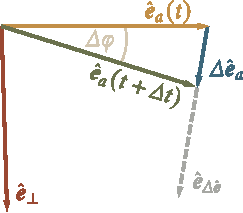
\includegraphics[scale=0.95]{figures/ch_01/fig_1_19.pdf}
		\caption[]{}
		\label{fig:1_19}
	\end{center}
\end{figure}

Đạo hàm của $\vecuni{a}$ theo $t$, theo định nghĩa, bằng
\begin{equation*}
\diff{\vecuni{a}}{t} = \lim_{\Delta t\to 0} \frac{\Delta\vecuni{a}}{\Delta t} = \lim_{\Delta t\to 0} \frac{\Delta\varphi}{\Delta t}\vecuni{\Delta\vec{e}} = \diff{\varphi}{t}\vecuni{\perp}.
\end{equation*}

\noindent
Như vậy,
\begin{equation}\label{eq:1_56}
\dot{\hat{\vec{e}}}_{a} = \dot{\varphi}\vecuni{\perp}.
\end{equation}

\noindent
Đại lượng $\dot{\varphi}=\diffin{\varphi}{t}$ là vận tốc góc quay của vector $\vec{a}$ (xem Sec.~\ref{sec:1_5}). Chuẩn $\vecuni{\perp}$ nằm trong mặt phẳng mà tại đó vector $\vec{a}$ bị quay tại thời điểm đã cho, hơn nữa hướng về phía mà sự quay xảy ra.

\section{Vận tốc}\label{sec:1_3}

Khi chuyển động, chất điểm vẽ một đường nào đó. Đường này được gọi là \textbf{quỹ đạo}\footnote{Ta hãy chú ý rằng khái niệm quỹ đạo chỉ được áp dụng cho hạt ``cổ điển'' mà tại mỗi thời điểm có thể gán cho nó các giá trị chính xác của tọa độ và xung lượng (tức là vận tốc). Theo cơ học lượng tử các hạt có thực có thể được đặc trưng bằng tọa độ và xung lượng chỉ với một độ chính xác nào đó. Giới hạn của độ chính xác này được xác định bằng hệ thức bất định Heisenberg: $\Delta x\Delta p\gtrsim\hbar$. Ở đây $\Delta x$ là độ bất định của tọa độ, $\Delta p$ là độ bất định của xung lượng của hạt, $\hbar$ là hằng số Planck có giá trị bằng $\hbar = h/2\pi = \SI{1.05e-34}{\joule\second}$. Dấu $\gtrsim$ nghĩa là ``lỡn hơn đại lượng vào cỡ''. Nếu thay xung lượng bằng tích khối lượng với vận tốc, thì có thể viết $\Delta x\Delta v\gtrsim\hbar/m$. Từ hệ thức này rõ ràng là khối lượng của hạt càng nhỏ thì tọa độ và vận tốc của nó càng kém được xác định và do đó khái niệm quỹ đạo càng ít được áp dụng. Đối với các vật vĩ mô (tức là các vật được tạo bởi một số rất lớn các phân tử) các độ bất định của tọa độ và vận tốc không vượt quá độ chính xác có thể đạt được trong thực tế khi đo các đại lượng này, do đó khái niệm quỹ đạo có thể áp dụng được cho các vật như thế một cách vô điều kiện. Đối với các hạt vi mô (các electron, proton, neutron, các nguyên tử và phân tử riêng lẻ) tùy thuộc vào các điều kiện trong đó chuyển động xảy ra, khái niệm quỹ đạo hoặc hoàn toàn không áp dụng được hoặc có thể áp dụng được với độ chính xác hạn chế. Chẳng hạn, sự chuyển động của các electron trong ống tia điện tử có thể được coi một cách gần đúng như chuyển động xảy ra theo các quỹ đạo nào đó.}.Tùy theo dạng của quỹ đạo người ta phân biệt chuyển động thẳng, chuyển động tròn, chuyển động cong, v.v...

\begin{figure}[!htb]
	\begin{minipage}[t]{0.5\linewidth}
		\begin{center}
			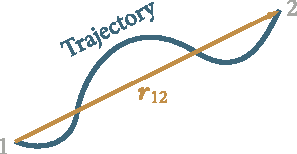
\includegraphics[scale=0.95]{figures/ch_01/fig_1_20.pdf}
			\caption[]{}
			\label{fig:1_20}
		\end{center}
	\end{minipage}
	\hfill{ }%\hspace{-0.1cm}
	\begin{minipage}[t]{0.5\linewidth}
		\begin{center}
			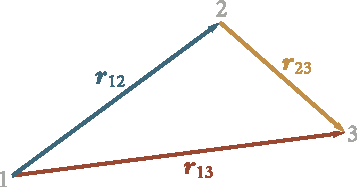
\includegraphics[scale=0.95]{figures/ch_01/fig_1_21.pdf}
			\caption[]{}
			\label{fig:1_21}
		\end{center}
	\end{minipage}
\end{figure}

Giả thử một chất điểm (Sau này để cho gọn ta sẽ gọi nó là một hạt) dịch chuyển dọc theo một quỹ đạo nào đó từ điểm $1$ đến điểm $2$ (\fig{1_20}). Khoảng cách giữa điểm $1$ và $2$ tính dọc theo quỹ đạo được gọi là quãng đường mà hạt đi qua. Ta ký hiệu nó bằng chữ $s$.

Đoạn thẳng vẽ từ điểm $1$ và $2$ được gọi là độ dời của hạt. Ta hãy ký hiệu nó bằng $\vec{r}_{12}$. Ta hãy giả sử rằng hạt thực hiện hai sự dịch chuyển nối tiếp nhau: $\vec{r}_{12}$ và $\vec{r}_{23}$ (\fig{1_21}). Gọi một cách tự nhiên độ dời $\vec{r}_{13}$ mà nó dẫn tới kết quả như hai sự dịch chuyển đầu tiên xảy ra cùng với nhau, là tổng của các độ dời này. Như vậy, các độ dời đều được đặc trưng bằng trị số và hướng và ngoài ra, đều cộng được theo quy tắc hình bình hành. Từ đó suy ra rằng độ dời là một vector.

Trong đời sống hàng ngày người ta hiểu vận tốc là quãng đường vật đi được trong một đơn vị thời gian. Nếu trong những khoảng thời gian bằng nhau và nhỏ tùy ý hạt đi qua những quãng đường như nhau, thì người ta gọi chuyển động của hạt là \textbf{chuyển động đều} . Trong trường hợp này, vận tốc của hạt tại mỗi thời điểm có thể tính bằng cách hcia quãng đường $s$ cho thời gian $t$.

Trong vật lý, người ta hiểu vận tốc là một đại lượng vector đặc trưng không chỉ cho độ nhanh của sự chuyển dời của hạt theo quỹ đạo mà cả cho hướng trong đó hạt chuyển động tại mỗi thời điểm. Ta hãy chia quỹ đạo thành các phần vô cùng nhỏ có độ dài $\mathrm{d}s$. Ta so sánh độ dời vô cùng nhỏ $\mathrm{d}r$ với mỗi phần đó (\fig{1_22}). Chia độ dời này cho khoảng thời gian tương ứng $\mathrm{d}t$, ta được vận tốc tức thời tại điểm đã cho của quỹ đạo:
\begin{equation}\label{eq:1_57}
\vec{v} = \diff{\vec{r}}{t} = \dot{\vec{r}}.
\end{equation}

\noindent
Như vậy vận tốc là đạo hàm của bán kính vector của hạt theo thời gian. Độ dời $\mathrm{d}r$ trùng với yếu tố quỹ đạo vô cùng nhỏ. Do đó vector $\vec{v}$ hướng theo tiếp tuyến của quỹ đạo (xem \fig{1_22}).

\begin{figure}[!htb]
	\begin{minipage}[t]{0.5\linewidth}
		\begin{center}
			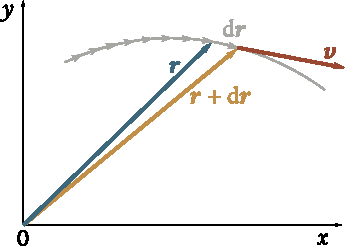
\includegraphics[scale=0.90]{figures/ch_01/fig_1_22.pdf}
			\caption[]{}
			\label{fig:1_22}
		\end{center}
	\end{minipage}
	\hfill{ }%\hspace{-0.1cm}
	\begin{minipage}[t]{0.5\linewidth}
		\begin{center}
			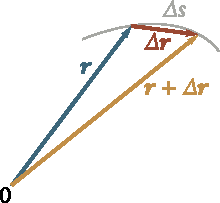
\includegraphics[scale=0.92]{figures/ch_01/fig_1_23.pdf}
			\caption[]{}
			\label{fig:1_23}
		\end{center}
	\end{minipage}
\end{figure}

Nếu lý luận một cách chặt chẽ hơn để có được công thức \eqref{eq:1_57} thì cần phải làm như sau. Bằng cách cố định một thời điểm $t$ nào đó, ta hãy nghiên cứu số gia $\Delta\vec{r}$ của bán kính vector trong khoảng thời gian nhỏ $\Delta t$\footnote{Ký hiệu $\Delta$ (delta) được dùng trong hai trường hợp: (a) để ký hiệu cho số gia của một đại lượng nào đó. Trong trường hợp đang xét, $\Delta\vec{r}$ là số gia của bán kính vector $\vec{r}$ trong thời gian $\Delta t$; (b) để ký hiệu cho một phần của một đại lượng nào đó. Chẳng hạn, $\Delta t$ là một phần của toàn bộ thời gian $t$ trong đó chuyển động xảy ra, $\Delta s$ là một phần của toàn bộ quãng đường $s$ mà hạt đi qua.} tiếp sau $t$ (\fig{1_23}). Tỷ số $\Delta\vec{r}/\Delta t$ cho giá trị trung bình của vận tốc trong khoảng thời gian $\Delta t$. Nếu lấy tất cả các khoảng $\Delta t$ nhỏ thì tỷ số $\Delta\vec{r}/\Delta t$ tại giới hạn cho ta giá trị của vận tốc $\vec{v}$ tại thời điểm $t$:
\begin{equation}\label{eq:1_58}
\vec{v} = \lim_{\Delta t\to 0} \frac{\Delta\vec{r}}{\Delta t} = \diff{\vec{r}}{t}.
\end{equation}

\noindent
Ta đi tới công thức\eqref{eq:1_57}.

Ta hãy tìm module của biểu thức \eqref{eq:1_58}, tức là module của vận tốc $\vec{v}$:
\begin{equation}\label{eq:1_59}
v = |\vec{v}| = \left|\lim_{\Delta t\to 0} \frac{\Delta\vec{r}}{\Delta t}\right| = \lim_{\Delta t\to 0} \frac{|\Delta\vec{r}|}{\Delta t}.
\end{equation}

\noindent
Trong công thức này không được viết $\Delta r$ thay cho $|\Delta\vec{r}|$. Vector $\Delta\vec{r}$ thực chất là hiệu của hai vector ($\vec{r}$ tại thời điểm $t+\Delta t$ trừ $\vec{r}$ tại thời điểm $t$). Do đó có thể viết module của nó bằng các vạch thẳng đứng [xem \eqn{1_2}]. Ký hiệu $|\Delta\vec{r}|$ có nghĩa là module của số gia của vector $\vec{r}$, trong khi mà $\Delta r$ là số gia của module của vector $\vec{r}$: $\Delta|\vec{r}|$. Cả hai đại lượng này nói chung không bằng nhau:
\begin{equation*}
|\Delta\vec{r}| \neq \Delta|\vec{r}| = \Delta r.
\end{equation*}

\noindent
Có thể thấy rõ điều này ở ví dụ sau. Giả sử vector $\vec{r}$ nhận số gia $\Delta\vec{r}$ sao cho module của nó không thay đổi: $|\vec{r}+\Delta\vec{r}|=|\vec{r}|$ (\fig{1_24}). Khi đó số gia của module của vector bằng không ($\Delta|\vec{r}| = \Delta r = 0$). Đồng thời module của số gia của vector $\vec{r}$, tức là $\Delta|\vec{r}|$, là khác không (nó bằng độ dài của đoạn $2-3$). Thật là đối với một vector $\vec{a}$ bất kỳ: trong trường hợp tổng quát $\Delta|\vec{a}|\neq\Delta|a|$.

\begin{figure}[!htb]
	\begin{center}
		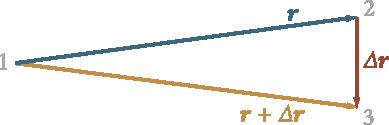
\includegraphics[scale=0.9]{figures/ch_01/fig_1_24.pdf}
		\caption[]{}
		\label{fig:1_24}
	\end{center}
\end{figure}

Từ \fig{1_23} rõ ràng là nói chung quãng đường $\Delta s$ về độ lớn khác với module của độ dời $|\Delta\vec{r}|$. Tuy nhiên nếu lấy đoạn đường $\Delta s$ là độ dời $\Delta\vec{r}$, tương ứng với tất cả khoảng thời gian $\Delta t$ nhỏ thì sự khác nhau giữa $\Delta s$ và $|\Delta\vec{r}|$ sẽ giảm và tỉ số của chúng tại giới hạn trở nên bằng đơn vị:
\begin{equation*}
\lim_{\Delta t\to 0} \frac{\Delta s}{|\Delta\vec{r}|} = 1.
\end{equation*}

\noindent
Trên cơ sở này, có thể thay thế $|\Delta\vec{r}|$ bằng $\Delta s$ trong công thức \eqref{eq:1_59}, kết quả là ta được biểu thức
\begin{equation}\label{eq:1_60}
v = \lim_{\Delta t\to 0} \frac{\Delta s}{\Delta t} = \diff{s}{t}.
\end{equation}

\noindent
Như vậy, module của vận tốc bằng đạo hàm của quãng đường theo thời gian.

Rõ ràng rằng, trong đời sống hàng ngày, đại lượng được gọi là vận tốc thật ralaf module của vận tốc $\vec{v}$. Trong chuyển động đều, module của vận tốc sẽ không đổi ($v=\text{constant}$), trong khi hướng của vector $\vec{v}$ biến đổi một cách tùy ý (trong trường hợp riêng có thể không đổi).

Theo công thức \eqn{1_57} độ dời nguyên tố của hạt bằng
\begin{equation}\label{eq:1_61}
\mathrm{d}\vec{r} = \vec{v}\,\mathrm{d}{t}.
\end{equation}

\noindent
Đôi khi để trực quan, ta ký hiệu độ dời nguyên tố bằng ký hiệu $\mathrm{d}\vec{s}$, nghĩa là viết \eqn{1_61} dưới dạng
\begin{equation}\label{eq:1_62}
\mathrm{d}\vec{s} = \vec{v}\,\mathrm{d}{t}.
\end{equation}

Có thể biểu diễn vector vận tốc cũng như mọi vector khác dưới dạng
\begin{equation}\label{eq:1_63}
\vec{v} = v_x\vecuni{x} + v_y\vecuni{y} + v_z\vecuni{z}
\end{equation}

\noindent
trong đó $v_x, v_y, v_z$ là các hình chiếu của vector $\vec{v}$ lên các trục tọa độ. Ngoài ra, the vector $\dot{\vec{r}}$ bằng $\vec{v}$ theo \eqn{1_43} có dạng như sau:
%\vspace{-12pt}
\begin{equation}\label{eq:1_64}
\dot{\vec{r}} = \dot{x}\vecuni{x} + \dot{y}\vecuni{y} + \dot{z}\vecuni{z}
\end{equation}

\noindent
So sánh các biểu thức \eqref{eq:1_63} và \eqref{eq:1_64} suy ra rằng
\begin{equation}\label{eq:1_65}
v_x = \dot{x},\quad v_y = \dot{y},\quad v_z = \dot{z}.
\end{equation}

\noindent
Do đó, hình chiếu của vector vận tốc lên trục tọa độ bằng đạo hàm theo thời gian của tọa độ tương ứng của hạt chuyển động. Nếu chú ý tới \eqref{eq:1_10} ta có công thức:
\begin{equation}\label{eq:1_66}
v = \sqrt{\dot{x}^2 + \dot{y}^2 + \dot{z}^2}.
\end{equation}

Có thể biểu diễn vector vận tốc dưới dạng $\vec{v}=v\vecuni{v}$, trong đó $v$ là module của vận tốc, còn $\vecuni{v}$ là chuẩn của vector $\vec{v}$. Ta hãy đưa vào chuẩn của tiếp tuyến với quỹ đạo là $\hatvec{\tau}$, quy ước hướng nó theo cùng một phía với $\vec{v}$. Khi đó, rõ ràng rằng các chuẩn $\vecuni{v}$ và $\hatvec{\tau}$ trùng nhau, cho nên có thể viết được biểu thức sau:
%\vspace{-12pt}
\begin{equation}\label{eq:1_67}
\vec{v} = v\vecuni{v} = v\hatvec{\tau}.
\end{equation}

Ta còn có một biểu thúc nữa đối với $\vec{v}$. Với mục đích này ta hãy đặt vào \eqn{1_57} bán kính vector dưới dạng $\vec{r}=r\vecuni{r}$. Theo \eqn{1_49}
\begin{equation}\label{eq:1_68}
\vec{v} = \dot{\vec{r}} = \dot{r}\vecuni{r} + r\dot{\hat{\boldsymbol{e}}}_r.
\end{equation}

\noindent
Để đơn giản hãy giới hạn ở trường hợp khi quỹ đạo là một đường cong phẳng, nghĩa là một đường cong mà mọi điểm của nó nằm trên một mặt phẳng. Ta hãy dùng mặt phẳng này làm mặt phẳng $x, y$. Trong \eqn{1_68}, vector $\vec{v}$ được biểu diễn dưới dạng tổng của hai thành phần (\fig{1_25}). Thành phần thứ nhất mà ta ký hiệu là $\vec{v}_r$ bằng
\begin{equation}\label{eq:1_69}
\vec{v}_r = \dot{r}\vecuni{r}.
\end{equation}

\begin{figure}[!htb]
	\begin{center}
		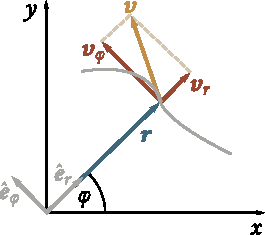
\includegraphics[scale=1]{figures/ch_01/fig_1_25.pdf}
		\caption[]{}
		\label{fig:1_25}
	\end{center}
\end{figure}


\noindent
Nó hướng dọc theo bán kính vector $\vec{r}$ và đặc trưng cho độ nhanh của sự biến đổi module của $\vec{r}$. Thành phần thú hai mà ta ký hiệu là $\vec{v}_{\varphi}$ bằng
\begin{equation}\label{eq:1_70}
\vec{v}_{\varphi} = r\dot{\hat{\boldsymbol{e}}}_r.
\end{equation}

\noindent
Nó đặc trưng cho độ nhanh của sự biến đổi về hướng của bán kính vector.

Dùng \eqn{1_56} có thể viết là
\begin{equation*}
\dot{\hat{\boldsymbol{e}}}_r = \diff{\varphi}{t}\vecuni{\varphi} = \dot{\varphi}\vecuni{\varphi}
\end{equation*}

\noindent
trong đó $\varphi$ là góc giữa bán kính vector và trục $x$, $\vecuni{\varphi}$ là chuẩn vuông góc với bán kính vector hướng về phía tăng của góc $\varphi$ [trong \eqn{1_56} chuẩn được ký hiệu là $\vecuni{\perp}$]. Thế giá gị này vào \eqn{1_70} ta có:
\begin{equation}\label{eq:1_71}
\vec{v}_{\varphi} = r\dot{\varphi}\vecuni{\varphi}.
\end{equation}

\noindent
Ta đưa vào các ký hiệu $\vec{v}_{\varphi}$ và $\vecuni{\varphi}$ để nhấn mạnh rằng thành phần $\vec{v}_{\varphi}$ và chuẩn tương ứng liên hệ với sự biến đổi của góc $\varphi$.

Rõ ràng rằng, các vector $\vec{v}_r$ và $\vec{v}_{\varphi}$ vuông góc với nhau. Do đó
\begin{equation}\label{eq:1_72}
v = \sqrt{v_r^2 + v_{\varphi}^2} = \sqrt{\dot{r}^2 + r^2\dot{\varphi}^2}.
\end{equation}

Ta hãy xét bài toán là khi biết độ lớn của vận tốc tại mỗi thời điểm, hãy tính quãng đường mà hạt đi qua từ thời điể $t_1$ đến thời điểm $t_2$. Ta chia khoảng thời gian $t_2-t_1$ thành $N$ khoảng nhỏ, không nhất thiết phải bằng nhau: $\Delta t_1$, $\Delta t_2$, \ldots, $\Delta t_N$. Có thể biểu diễn toàn bộ quãng đường $s$ mà hạt đi được như là tổng các quãng đường $\Delta s_1$, $\Delta s_2$, \ldots, $\Delta s_N$ mà hạt đi được trong những khoảng thời gian $\Delta t$ tương ứng:
\begin{equation*}
s = \Delta s_1 + \Delta s_2 + \ldots + \Delta s_N = \sum_{i=1}^{N} \Delta s_i.
\end{equation*}

\noindent
Theo \eqn{1_60}, mỗi số hạng có thể biểu diễn gần đúng dưới dạng
\begin{equation*}
\Delta s_i \approx v_i \Delta t_i
\end{equation*}

\noindent
trong đó $\Delta t_i$ là khoảng thời gian mà hạt đi được một quãng đường $\Delta s_i$, còn $v_i$ là giá trị của vạn tốc trong khoảng thời gian $\Delta t_i$. Do đó
\begin{equation}\label{eq:1_73}
s \approx \sum_{i=1}^{N} v_i \Delta t_i.
\end{equation}

\noindent
Đằng thức trên càng chính xác nếu khoảng thời gian $\Delta t_i$ càng nhỏ. Tại giới hạn khi tất cả các khoảng $\Delta t_i$ tiến tới không (số lượng các khoảng $\Delta t_i$ khi đó tăng vô hạn) thì đẳng thức gần đúng trở thành đẳng thức đúng:
\begin{equation*}
s = \lim_{\Delta t_i\to 0} \sum_{i=1}^{N} v_i \Delta t_i.
\end{equation*}

Biểu thức thu được là một tích phân xác định của hàm $v(t)$ lấy trong phạm vi từ $t_1$ đến $t_2$. Như vậy, quãng đường mà hạt đi được trong khoảng thời gian từ $t_1$ đến $t_2$ bằng
\begin{equation}\label{eq:1_74}
s = \int_{t_1}^{t_2} v(t)\,\mathrm{d}t.
\end{equation}

\noindent
Ta hãy nhấn mạnh rằng ở đây nói về module của vận tốc. Nếu lấy tích phân của chính vận tốc $\vec{v}(t)$ thì người ta thu được vector độ dời của hạt tử điểm mà hạt nằm ở thời điểm $t_1$ tới điểm mà hạt nằm ở thời điểm $t_2$:
\begin{equation}\label{eq:1_75}
\int_{t_1}^{t_2} v(t)\,\mathrm{d}t = \int_{t_1}^{t_2} \mathrm{d}\vec{r} = \vec{r}_{12}
\end{equation}

\noindent
[xem \eqn{1_61}].

Nếu vẽ đồ thị biểu diễn sự phụ thuộc của $v$ theo $t$ (\fig{1_26}) thì có thể biểu diễn quãng đường đi được như diện tích của hình được giwois hạn bởi đường cong $v(t)$ và các đường thẳng $t = t_1$ và $t = t_2$. Thật vậy, tích $v_i\Delta t_i$ nvề trị số bằng diện tích của dải thứ $i$. Tổng \eqn{1_73} bằng diện tích được giới hạn về phía trên bởi đường gấp khúc tạo bởi các mép trên của tất cả các dải tương tự. Khi tất cả $\Delta t_i$ tiến tới không độ rộng của các dải giảm (đồng thời số các dải tăng) và đường gấp khúc tại giới hạn trùng với đường cong $v = v(t)$. Như vậy quãng đường đi được trong thời điểm $t_1$ đến thời điểm $t_2$ về trị số bằng diện tích giới hạn bởi đồ thị của hàm $v = v(t)$, trục thời gian $t$ và các đường thẳng $t= t_1$ và $t = t_2$.

\begin{figure}[!htb]
	\begin{center}
		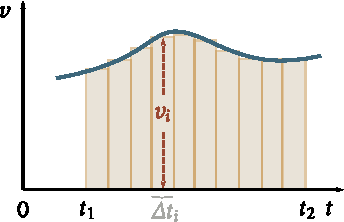
\includegraphics[scale=1]{figures/ch_01/fig_1_26.pdf}
		\caption[]{}
		\label{fig:1_26}
	\end{center}
\end{figure}

Ta hãy chú ý rằng giá trị trung bình của module của vận tốc trong khoảng thời gian từ $t_1$ đến  $t_2$ theo định nghĩa bằng
\begin{equation*}
\average{v} = \frac{s}{t_2-t_1}.
\end{equation*}

\noindent
(The symbol $\langle\rangle$ embracing the $v$ indicates an average.) Thay thế biểu thức \eqref{eq:1_74} đối với $s$ vào đây ta có:
\begin{equation}\label{eq:1_76}
\average{v} = \frac{1}{t_2-t_1}\,\int_{t_1}^{t_2}v(t)\,\mathrm{d}t.
\end{equation}

\noindent
Người ta tính các giá trị trung bình của các hàm vô hướng hay các hàm vector bất kỳ cũng tương tự như vật. Chẳng hạn, giá trị trung bình của vận tốc bằng
\begin{equation}\label{eq:1_77}
\average{\vec{v}} = \frac{1}{t_2-t_1}\,\int_{t_1}^{t_2}\vec{v}(t)\,\mathrm{d}t = \frac{\vec{r}_{12}}{t_2-t_1}.
\end{equation}

\noindent
[xem \eqn{1_75}]. Các giá trị trung bình của hàm $y(x)$ trong khoảng từ $x_1$ đến $x_2$ được xác định bằng biểu thức
\begin{equation}\label{eq:1_78}
\average{y} = \frac{1}{t_2-t_1}\,\int_{x_1}^{x_2}y(t)\,\mathrm{d}x.
\end{equation}

\section{Gia tốc}\label{sec:1_4}

Vận tốc $\vec{v}$ của hạt có thể biến đổi theo thời gian cả về độ lớn lẫn hướng. Độ nhanh của sự thay đổi của vector $\vec{v}$ cũng như độ nhanh của sự thay đổi của một hàm bất kỳ của thời gian được định nghĩa bằng đạo hàm của vector $\vec{v}$ theo $t$. Nếu ký hiệu đạo hàm này bằng chữ $\vec{a}$ thì ta có:
\begin{equation}\label{eq:1_79}
\vec{a} = \lim_{\Delta t\to 0}\frac{\Delta\vec{v}}{\Delta t} = \diff{\vec{v}}{t} = \dot{\vec{v}}.
\end{equation}

\noindent
Đại lượng xác định bằng công thức \eqref{eq:1_79} được gọi là \textbf{gia tốc} của hạt.

Ta chú ý rằng vector $\vec{v}$ có vai tròn như thế nào đối với bán kính vector $\vec{r}$ thì gia tốc $\vec{a}$ có vai trò như thế đối với $\vec{v}$.

Các vector bằng nhau có hình chiếu lên các trục tọa độ như nhau. Do đó, chẳng hạn
\begin{equation*}
a_x = \left(\diff{\vec{v}}{t}\right)_{\text{pr. }\vec{x}} = \diff{v_x}{t} = \dot{v}_x
\end{equation*}

\noindent
[xem Eqs.~\eqref{eq:1_40}]. Đồng thời, theo Eqs.~\eqref{eq:1_65}, we have $v_x=\dot{x}=\diffin{x}{t}$. Do đó
\begin{equation*}
\diff{v_x}{t} = \frac{\mathrm{d}}{\mathrm{d}t} \left(\diff{x}{t}\right) = \diffsec{x}{t} = \ddot{x}.
\end{equation*}

\noindent
Ta đã có hình chiếu của vector gia tốc lên trục $x$ bằng đạo hàm bậc hai của tọa độ x theo thời gian: $a_x=\ddot{x}$. Một cách tương tự, người ta cũng có được các biểu thức đối với hình chiếu của gia tốc lên các trục $y$ và $z$. Như vậy,
\begin{equation}\label{eq:1_80}
a_x=\ddot{x},\quad a_y=\ddot{y},\quad a_z=\ddot{z}.
\end{equation}

Ta hãy thay thế \eqn{1_67} đối với $\vec{v}$  vào công thức \eqref{eq:1_79}:
\begin{equation}\label{eq:1_81}
\vec{a} = \diff{(v\hatvec{\tau})}{t}.
\end{equation}

\noindent
Ta nhớ rằng $\hatvec{\tau}$ là chuẩn của tiếp tuyến với quỹ đạo, hướng về cùng phía với $\vec{v}$. Theo \eqn{1_49},
\begin{equation}\label{eq:1_82}
\vec{a} = \dot{v}\hatvec{\tau} + v\dot{\hatvec{\tau}}.
\end{equation}

\noindent
Do đó có thể biểu diễn vector $\vec{a}$ dưới dạng tổng của hai thành phần. Một thành phần cùng phương với $\hatvec{\tau}$, tức là hướng theo tiếp tuyến với quỹ đạo, và do đó được ký hiệu là $\vec{a}_{\hatvec{\tau}}$ và được gọi là \textbf{gia tốc tiếp tuyến}. Nó bằng
\begin{equation}\label{eq:1_83}
\vec{a}_{\hatvec{\tau}} = \dot{v}\hatvec{\tau}.
\end{equation}

\noindent
Thành phần thứ hai bằng $v\dot{\hatvec{\tau}}$, như ta sẽ chứng tỏ ở dưới đây, hướng theo pháp tuyến với quỹ đạo và do đó được ký hiệu là $\vec{a}_{\hatvec{n}}$ và được gọi là \textbf{gia tốc pháp tuyến}. Như vậy,
\begin{equation}\label{eq:1_84}
\vec{a}_{\hatvec{n}} = v\dot{\hatvec{\tau}}.
\end{equation}

Ta hãy nghiên cứu các tính chất của cả hai thành phần, để đơn giản chỉ bó hẹp ở trường hợp khi quỹ đạo là một đường cong phẳng.

Module của gia tốc tiếp tuyến \eqref{eq:1_83} bằng
\begin{equation}\label{eq:1_85}
\vec{a}_{\hatvec{\tau}} = |\dot{v}|.
\end{equation}

\noindent
Nếu $\dot{v}>0$ (vận tốc tăng về độ lớn), thì vector $\vec{a}_{\hatvec{\tau}}$ có cùng hướng với $\hatvec{\tau}$ (tức là có cùng hướng với $\vec{v}$). Nếu $\dot{v}<0$ (vận tốc giảm theo thời gian), thì các vector $\vec{v}$ và $\vec{a}_{\hatvec{\tau}}$ hướng theo các chiều ngược nhau. Trong chuyển đông đều $\dot{v}=0$, và do đó không có gia tốc tiếp tuyến.

Để làm rõ các tính chất của gia tốc pháp tuyển [\eqn{1_84}] cần phải xác minh xem $\dot{\hatvec{\tau}}$, tức là độ nhanh của sự thay đổi theo thời gian của hướng tiếp tuyến với quỹ đạo, sẽ được xác định bằng cái gì. Dễ dàng hiểu được rằng độ nhanh này sẽ càng lớn khi độ cong của quỹ đạo càng lớn và khi hạt dịch chuyển càng nhanh theo quỹ đạo.

Mức độ cong của đường cong phẳng được đặc trưng bằng độ cong $C$, mà nó được định nghĩa bằng biểu thức
\begin{equation}\label{eq:1_86}
C = \lim_{\Delta t\to 0} \frac{\Delta\varphi}{\Delta s} = \diff{\varphi}{s}
\end{equation}

\noindent
trong đó $\Delta\varphi$ là góc giữa các tiếp tuyến với đường cong tại các điểm cách nhau một khoảng $\Delta s$ (\fig{1_27}). Như vậy độ cong xác định vận tốc quay của tiếp tuyến khi dịch chuyển dọc theo đường cong.

\begin{figure}[!htb]
	\begin{center}
		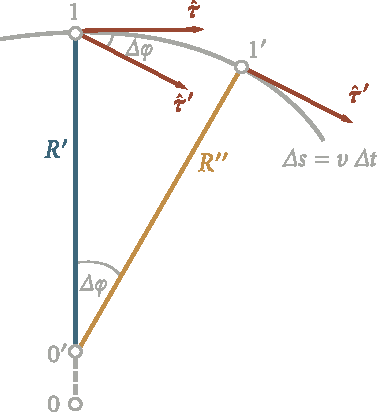
\includegraphics[scale=1]{figures/ch_01/fig_1_27.pdf}
		\caption[]{}
		\label{fig:1_27}
	\end{center}
\end{figure}


Đại lượng nghịch đảo của độ cong $C$ được gọi là \textbf{bán kính cong} của đường cong tại điểm đã cho và được ký hiệu bằng chữ $R$:
The degree of bending of a plane curve is characterized by its curvature $C$ determined by the expression
\begin{equation}\label{eq:1_87}
R = \frac{1}{C} = \lim_{\Delta\varphi\to 0} \frac{\Delta s}{\Delta\varphi} = \diff{s}{\varphi}.
\end{equation}

\noindent
Bán kính cong là bán kính của một đường tròn mà nó nhập vào đường cong tại một phần vô cùng nhỏ của nó ở điểm đã cho. Tâm của đường tròn này được gọi là tâm cong đối với điểm đã cho của đường cong.

Bán kính cong và tâm cong tại điểm $1$ (xem \fig{1_27}) Có thể được xác định bằng cách sau. Ta hãy lấy điểm $1'$ không xa $1$. Vẽ các tiếp tuyến $\hatvec{\tau}$ và $\hatvec{\tau}'$ tại các điểm này. Các đường thẳng vuông góc với các tiếp tuyến cắt nhau tại một điểm $0'$. Ta chú ý rằng đối với một đường cong không phải là đường tròn, các khoảng cách $R'$ và $R''$ sẽ khác nhau rất ít. Nếu dịch điểm $1'$ lại gần điểm $1$, thì giao điểm $0'$ của các đường vuông góc sẽ dịch chuyển dọc theo đường thẳng $R'$ và tại giới hạn nó nằm tại một điểm $0$ nào đó. Chính điểm này là tâm cong đối với điểm $1$. Các khoảng cách $R'$ và $R"$ sẽ tiến đến một giới hạn chung $R$ bằng bán kính cong. Thực vậy, nếu các điểm $1$ và $1'$ ở gần nhau thì có thể viết là $\Delta\varphi\approx\Delta s/R'$ or $R' \approx \Delta s/\Delta\varphi$. Tại giới hạn khi $\Delta\varphi\to 0$ thì đẳng thức gần đúng này chuyển về đẳng thức thực sự $R=\diffin{s}{\varphi}$, trùng với định nghĩa của bán kính cong [xem \eqn{1_87}].

Ta hãy trở lại cách tính $\vec{a}_{\hatvec{n}}$ [xem \eqn{1_84}]. Theo \eqn{1_56},
\begin{equation}\label{eq:1_88}
\dot{\hatvec{\tau}} = \diff{\varphi}{t}\hatvec{n}
\end{equation}

\noindent
trong đó $\hatvec{n}$ là chuẩn của pháp tuyến với quỹ đạo, hướng về phía mà khi hạt chuyển động theo quỹ đạo thì vector $\hatvec{\tau}$ quay về phía đó [trong \eqn{1_56} chuẩn tương tự đã được ký hiệu bằng $\vecuni{\perp}$]. Có thể liên kết đại lượng $\diffin{\varphi}{t}$ với bán kính cong của quỹ đạo và vận tốc $\vec{v}$ của hạt. Từ \fig{1_27} suy ra rằng
\begin{equation*}
\Delta\varphi\approx \frac{\Delta s}{R'} = \frac{v'\,\Delta t}{R'}
\end{equation*}

\noindent
trong đó $\Delta\varphi$ là góc quay của vector $\hatvec{\tau}$ trong khoảng thời gian $\Delta t$ (trùng với góc giữa các đường vuông góc $R'$ và $R''$), $v'$ là vận tốc trung bình trên quãng đường $\Delta s$. Từ đây
\begin{equation*}
\frac{\Delta\varphi}{\Delta s} \approx \frac{v'}{R'}.
\end{equation*}

\noindent
Tại giới hạn khi $\Delta t\to 0$ không đẳng thức gần đúng trở thành đẳng thức thực sự, vạn tốc trung bình $v'$ trở thành vận tốc tức thời $v$ tại thời điểm $1$, $R'$ trở thành bán kính cong $R$. Kết quả là ta có đẳng thức
\begin{equation}\label{eq:1_89}
\diff{\varphi}{t} = \frac{v}{R} = vC
\end{equation}

\noindent
($C$ là độ cong).Do đó độ nhanh của sự quay vector vận tốc, như ta đã giả thử, sẽ tỷ lệ với độ cong của quỹ đạo và vận tốc chuyển dời của hạt theo quỹ đạo.

Thay \eqn{1_89} vào \eqref{eq:1_88} ta được $\dot{\hatvec{\tau}}=(v/R)\hatvec{n}$. Sau cùng, introducing thay biểu thúc này vào \eqn{1_84}, ta đi tới công thức cuối cùng đối vwois gia tốc pháp tuyến:
%\vspace{-12pt}
\begin{equation}\label{eq:1_90}
\vec{a}_{\hatvec{n}} = \diff{v^2}{R}\hatvec{n}.
\end{equation}

Vậy vector gia tốc khi hạt chuyển động theo đường cong phẳng được xác định bởi biểu thức sau:
\begin{equation}\label{eq:1_91}
\vec{a} = \vec{a}_{\hatvec{\tau}} + \vec{a}_{\hatvec{n}} = \dot{v}\hatvec{\tau} + \frac{v^2}{R}\hatvec{n}.
\end{equation}

\noindent
Module của vector $\vec{a}$ bằng
\begin{equation}\label{eq:1_92}
a = \sqrt{a_{\hatvec{\tau}}^2 + a_{\hatvec{n}}^2} = \sqrt{\dot{v}^2 + \left(\frac{v^2}{R}\right)^2}.
\end{equation}

Trong chuyển động thẳng gia tốc pháp tuyến không có mặt. Ta hãy chú ý rằng $\vec{a}_{\hatvec{n}}$ triệt tiêu tại điểm uốn của quỹ đạo cong (tại điểm IP trên \fig{1_28}). Về cả hai bên của điểm này các vector $\vec{a}_{\hatvec{n}}$ hướng về các phía khác nhau. Vector $\vec{a}_{\hatvec{n}}$ không thể biến đổi nhảy vọt; sự thay đổi hướng ngược lại xảy ra một cách đều đặn với sự triệt tiêu của $\vec{a}_{\hatvec{n}}$ tại điểm uốn. Giả sử hạt chuyển động đều với gia tốc không thay đổi về độ lớn nên $\vec{a}_{\hatvec{\tau}}=0$, cho nên $\vec{a}=\vec{a}_{\hatvec{n}}$. Sự không thay đổi về độ lớn của $\vec{a}_{\hatvec{n}}$ có nghĩa là $v^2/R=\text{constant}$. Từ đó ta kết luận rằng $R=\text{constant}$ ($v=\text{constant}$ do chuyển động đều). Như thế là, hạt chuyển động theo đường cong có độ cong không đổi, tức là theo đường tròn. Vì vậy trong trường hợp mà gia tốc của hạt không đổi về độ lớn và tại mỗi thời điểm được hướng vuông góc với vector vận tốc, thì đường tròn là quỹ đạo của hạt.

\begin{figure}[!htb]
	\begin{center}
		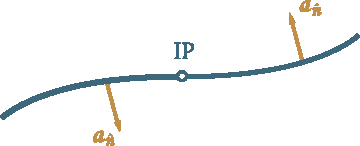
\includegraphics[scale=0.95]{figures/ch_01/fig_1_28.pdf}
		\caption[]{}
		\label{fig:1_28}
	\end{center}
\end{figure}

\section{Động học của chuyển động quay}\label{sec:1_5}

Có thể biểu diễn sự quay một vật một góc $\varphi$ nào đó dưới dạng một đoạn thẳng có độ dài bằng $\varphi$, còn hướng trùng với trục quay. Để chỉ ra phép quay xung quanh trục đã cho được thực hiện theo chiều nào, người ta gắn chiều quay và đoạn thẳng biểu diễn nó bằng \textbf{quy tắc cái đinh ốc thuận}: chiều của đoạn thẳng phải như thế nào để khi nhìn dọc theo nó (\fig{1_29}) ta thấy sự quay được thực hiện theo chiều kim đồng hồ (khi quay đầu đinh ốc thuận theo chiều kim đồng hồ ta làm cho nó dịch chuyển theo chính nó). Trong \ref{sec:1_2} đã chứng tỏ (xem \fig{1_4}) rằng các sự quay những góc hữu hạn được cộng không theo quy tắc hình bình hành và do đó không là những vector. Đối với các sự quay các góc rất nhỏ $\Delta\vec{\varphi}$ thì lại khác. Quãng đường mà một điểm bất kỳ của vật đi được trong sự quay rất nhỏ có thể được coi là quãng đường thẳng (\fig{1_30}). Do đó hai sự quay nhỏ $\Delta\vec{\varphi}_1$ và $\Delta\vec{\varphi}_2$ được thực hiện liên tiếp, như đã thấy trên hình vẽ, gây ra cùng một sự dịch chuyển $\Delta\vec{r}_3=\Delta\vec{r}_1+\Delta\vec{r}_2$ của một điểm bất kỳ của vật như sự quay $\Delta\vec{\varphi}_3$ thu được từ $\Delta\vec{\varphi}_1$ và $\Delta\vec{\varphi}_2$ bằng cách cộng theo quy tắc hình bình hành. Từ đó suy ra rằng có thể coi các sự quay rất nhỏ như các vector (ta ký hiệu các vector này bằng ký hiệu $\Delta\vec{\varphi}$ hoặc $\mathrm{d}\vec{\varphi}$). Hướng của vector quay gắn liền với hướng quay của vật. Do đó $\mathrm{d}\vec{\varphi}$ không là một vector thực mà là một giả vector.

\begin{figure}[!htb]
	\begin{minipage}[t]{0.5\linewidth}
		\begin{center}
			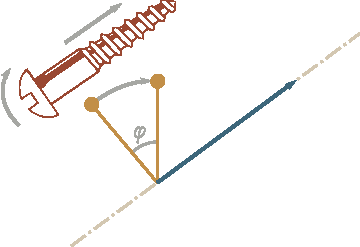
\includegraphics[scale=0.95]{figures/ch_01/fig_1_29.pdf}
			\caption[]{}
			\label{fig:1_29}
		\end{center}
	\end{minipage}
	\hfill{ }%\hspace{-0.1cm}
	\begin{minipage}[t]{0.5\linewidth}
		\begin{center}
			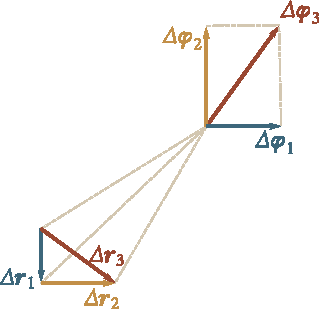
\includegraphics[scale=0.95]{figures/ch_01/fig_1_30.pdf}
			\caption[]{}
			\label{fig:1_30}
		\end{center}
	\end{minipage}
\end{figure}

Đại lượng vector
\begin{equation}\label{eq:1_93}
\vec{\omega} = \lim_{\Delta t\to 0} \frac{\Delta\vec{\varphi}}{\Delta t} = \diff{\vec{\varphi}}{t}
\end{equation}

\noindent
(trong đó $\Delta t$ là thời gian mà sự quay $\Delta\vec{\varphi}$ được thực hiện) được gọi là vận tốc góc của vật\footnote{Vận tốc $\vec{v}$  được khảo sát trong \ref{sec:1_3} đôi khi được gọi là vận tốc dài.}. Vận tốc góc $\vec{\omega}$ hướng dọc theo trục quay của vật theo chiều được xác định bằng quy tắc cái đinh ốc thuận (\fig{1_31}) và là một giả vector. Module của vận tốc góc bằng $\diffin{\varphi}{t}$. Sự quay với vận tốc góc không đổi được gọi là sự quay đều. Nếu sự quay là đều thì $\omega=\varphi t$, trong đó $\varphi$ là góc quay hữu hạn trong thời gian $t$ (so sánh với $v=s/t$). Như vậy trong sự quay đều, $\omega$ chỉ rõ vật quay được góc nào trong một đơn vị thời gian.

\begin{figure}[!htb]
	\begin{minipage}[t]{0.5\linewidth}
		\begin{center}
			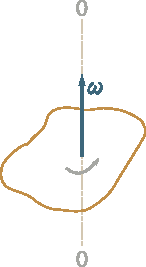
\includegraphics[scale=1]{figures/ch_01/fig_1_31.pdf}
			\caption[]{}
			\label{fig:1_31}
		\end{center}
	\end{minipage}
	\hspace{-0.1cm}
	\begin{minipage}[t]{0.5\linewidth}
		\begin{center}
			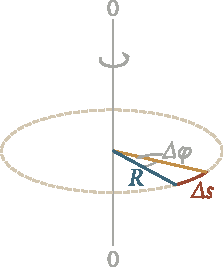
\includegraphics[scale=0.95]{figures/ch_01/fig_1_32.pdf}
			\caption[]{}
			\label{fig:1_32}
		\end{center}
	\end{minipage}
	\vspace{-0.5cm}
\end{figure}

Có thể đặc trưng sự quay đều bằng chu kỳ quay $T$, được hiểu là thời gian trong đó vật quay một vòng, nghĩa là quay một góc $2\pi$. Vì khoảng thời gian $\Delta t=T$ ứng với góc quay $\Delta\varphi=2\pi$, nên
\begin{equation}\label{eq:1_94}
\omega = \frac{2\pi}{T}
\end{equation}

\noindent
từ đó
\begin{equation}\label{eq:1_95}
T = \frac{2\pi}{\omega}.
\end{equation}

Số vòng $\nu$ trong một đơn vị thời gian rõ ràng bằng
\begin{equation}\label{eq:1_96}
\nu = \frac{1}{T} = \frac{\omega}{2\pi}.
\end{equation}

\noindent
Từ \eqn{1_96} suy ra rằng vận tốc góc sẽ bằng $2\pi$ nhân với số vòng trong một đơn vị thời gian:
\begin{equation}\label{eq:1_97}
\omega = 2\pi\nu.
\end{equation}

Có thể giữ nguyên khái niệm chu kỳ quay và số vòng trong một đơn vị thời gian cho cả sự quay không đều bằng cách hiểu giá trị tức thời $T$ là thời gian mà vật có thể thực hiện một vòng nếu nó quay đều với giá trị tức thời đã cho của vận tốc góc, còn $\nu$ được hiểu là số vòng mà vật thực hiện trong một đơn vị thời gian trong những điều kiện tương tự.

Vector $\vec{\omega}$ có thể biến đổi do sự biến đổi của vận tốc quay của vật xung quanh một trục (trong tường hợp này nó biến đổi về độ lớn) cũng như do sự quay của trục quay trong không gian (trong trường hợp này $\vec{\omega}$ biến đổi về hướng). Giả sử trong thời gian $\Delta t$, vector $\vec{\omega}$ nhận số gia $\Delta\vec{\omega}$. Sự biến đổi của vector vận tốc góc theo thời gian được đặc trưng bằng đại lượng
\begin{equation}\label{eq:1_98}
\vec{\alpha} = \lim_{\Delta t\to 0} \frac{\Delta\vec{\omega}}{t} = \diff{\vec{\omega}}{t}
\end{equation}

\noindent
được gọi là \textbf{gia tốc góc}. Gia tốc góc cũng như vận tốc góc là một giả vector.

\begin{figure}[!htb]
	\begin{center}
		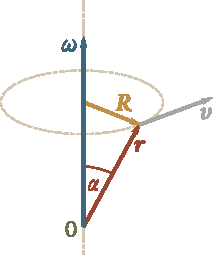
\includegraphics[scale=1]{figures/ch_01/fig_1_33.pdf}
		\caption[]{}
		\label{fig:1_33}
	\end{center}
\end{figure}

Các điểm riêng biệt của một vật quay sẽ có các vận tóc dài $\vec{v}$ khác nhau. Vận tốc của từng điểm biến đổi phương liên tục. Độ lớn $v$ của vận tốc được xác định bằng vận tốc quay $\omega$ của vật và khoảng cách $R$ từ điểm được xét đến trục quay. Giả sử trong khoảng thời gian nhỏ vật quay được một góc $\Delta\varphi$ (\fig{1_32}). Đồng thời điểm ằm cách trục một khoảng $R$ sẽ đi được một quãng đường $\Delta s=R\Delta\varphi$. Vận tốc dài của điểm sẽ bằng
\begin{equation*}
v = \lim_{\Delta t\to 0} \frac{\Delta s}{\Delta t} = \lim_{\Delta t\to 0} R\frac{\Delta\varphi}{\Delta t} = R \lim_{\Delta t\to 0} \frac{\Delta\varphi}{\Delta t} = R\diff{\varphi}{t} = R\omega.
\end{equation*}

\noindent
Như vậy
\begin{equation}\label{eq:1_99}
v = \omega R.
\end{equation}

Công thức \eqref{eq:1_99} liên hệ các module của vận tốc dài và vận tốc góc. Ta hãy tìm biểu thức liên hệ các vector $\vec{v}$ và $\vec{\omega}$. Vị trí của điểm đang xét của vật sẽ được xác định bằng bán kính vector $\vec{r}$ vẽ từ gốc tọa độ $O$ nằm trên trục quay (\fig{1_33}). Từ hình vẽ ta thấy rằng tích vector $\vecprod{\omega}{r}$ trùng về hướng tới vector $\vec{v}$ và có module bằng $\omega r\sin\alpha=\omega R$. Do đó,
\begin{equation}\label{eq:1_100}
\vec{v} = \vecprod{\omega}{r}.
\end{equation}

Module của gia tốc pháp tuyến của các điểm của vật quay bằng $\vec{a}_{\hatvec{n}}=v^2/R$. Thế giá trị $v$ từ \eqn{1_99} vào đây ta có
\begin{equation}\label{eq:1_101}
a_{\hatvec{n}} = \omega^2 R.
\end{equation}

\noindent
Nếu đưa vào vector $\vec{R}$ vuông góc với trục quay, vẽ từ điểm đã cho của vật (xem \fig{1_33}), thì có thể viết \eqn{1_101} dưới dạng vector:
\begin{equation}\label{eq:1_102}
\vec{a}_{\hatvec{n}} = -\omega^2 \vec{R}.
\end{equation}

\noindent
Trong công thức này có dấu trừ bởi vì các vector $\vec{a}_{\hatvec{n}}$ và $\vec{R}$ có các chiều ngược nhau.

Ta hãy giả thử rằng trục quay của vật không quay trong không gian. Theo \eqn{1_85} module của gia tốc tiếp tuyến bằng $|\diffin{v}{t}|$. Sử dụng hệ thức \eqref{eq:1_99} và chú ý đến khoảng cách $R=\text{constant}$ từ điểm đang xét của vật đến trục quay, có thể viết
\begin{equation*}
a_{\hatvec{\tau}} = \left| \lim_{\Delta t\to 0} \frac{\Delta v}{\Delta t} \right| = \left| \lim_{\Delta t\to 0} \frac{\Delta(\omega R)}{\Delta t} \right| = R \left| \lim_{\Delta t\to 0} \frac{\Delta(\omega)}{\Delta t} \right| = R\alpha
\end{equation*}

\noindent
trong $\alpha$ là module của gia tốc góc. Do đó module của gia tốc tiếp tuyến liên hệ với module của gia tốc góc bằng hệ thức:
\begin{equation}\label{eq:1_103}
a_{\hatvec{\tau}} = \alpha R.
\end{equation}

Như vậy gia tốc pháp tuyến và tiếp tuyến tăng tuyến tính với sự tăng của khoảng cách từ điểm tới trục quay.

% \cleardoublepage
% % !TEX root = saveliev_physics_general_course_1.tex
%!TEX TS-program = pdflatex
%!TEX encoding = UTF-8 Unicode


\chapter{ĐỘNG LỰC HỌC CỦA CHÁT ĐIỂM}\label{chap:2}

\section{Cơ học cổ điển. Phạm vi ứng dụng của nó}\label{sec:2_1}

Động học mô tả sự chuyển động của vật nhưng chưa đề cập tới vấn đề là tại sao vật lại chuyển động như thế này (chẳng hạn, chuyển động tròn đều hoặc thẳng nhanh dần đều) mà không như thế kia.

Động lực học nghiên cứu sự chuyển động của vật liên hệ với các nguyên nhân (các tương tác giữa các vật) gây ra một đặc trưng nào đó của chuyển động.

Ba định luật động lực học đã được Newton trình bày vào năm 1687 làm cơ sở của cơ học cổ điển hoặc cơ học Newton.

Các định luật Newton (cũng như tất cả các định luật vật lý còn lại) đã xuất hiện do sự khái quát hóa một số lượng lớn các sự kiện thực nghiệm. Sự đúng đắn của chúng (tuy đối với một phạm vi rất rộng lớn nhưng vẫn còn rất hạn chế của các hiện tưởng) được xác nhận bằng sự phù hợp giữa thí nghiệm với những kết luận rút ra từ những định luật đó.

Cơ học Newton đã đạt được nhiều thành tựu to lớn suốt trong hai thế kỷ, đến nỗi nhiều nhà vật lý của thế kỷ XIX đã tin vào sức mạnh toàn năng của nó. Người ta đã cho rằng giải thích một hiện tượng vật lý bất kỳ có nghĩa là đưa nó về một quá trình cơ học tuân theo các định luật Newton. Tuy nhiên với sự phát triển của khoa học người ta đã phát hiện ra các sự kiện mới không nằm trong phạm vi của cơ học cổ điển. Những sự kiện này đã được giải thích trong các thuyết mới là thuyết tương đối hẹp và cơ học lượng tử.

Trong thuyết tương đối hẹp, do Einstein xây dựng vào năm 1905, người ta đã xét lại tận gốc các quan niệm của Newton về không gian và thời gian. Sự xét lại này đã đưa tới việc xây dựng ``môn cơ học các vận tốc lớn'' hoặc như người ta gọi nó là cơ học tương đối tính. Tuy nhiên môn cơ học mới này không dẫn đến sự phủ nhận hoàn toàn môn cơ học Newton đã có. Các phương trình cơ học tương đối tính lại giới hạn (đối với các vận tốc nhỏ hơn vận tốc ánh sáng) đều chuyển thành các phương trình cơ học cổ điển. Như vậy, cơ học cổ đển đã nằm trong cơ học tương đối tính như một trường hợp riêng của nó và vẫn giữ nguyên tác dụng trước đây của nó đối với việc mô tả các chuyển động xảy ra với các vận tốc nhỏ.

Tình hình cũng tương tự đối với sự liên hệ giữa cơ học cổ điển và cơ học lượng tử ra đời tỏng những năm hai mươi của thế kỷ chúng ta do sự phát triển của vật lý nguyên tử. Các phương trình cơ học lượng tử tại giới hạn cũng cho (đối với các khối lượng lớn hơn khối lượng nguyên tử) các phương trình cơ học cổ điển. Do đó cơ học cổ điện cũng nằm trong cơ học lượng tử như là một trường hợp giới hạn của nó.

Như vậy, sự phát triển của khoa học đã không xóa bỏ cơ học cổ điển mà chỉ chứng tỏ sự ứng dụng hạn chế của nó. Cơ học cổ điện dựa trên các định luậ Newton là môn cơ học của các vật có các khối lượng lớn (so với khối lượng nguyên tử), chuyển động với các vận tốc nhỏ (so với vận tốc ánh sáng).

\section{Định luật Newton thứ nhất. Các hệ quy chiếu quán tính}\label{sec:2_2}

Định luật Newton thứ nhất được phát biểu như sau: \textit{mọi vật ở trạng thái nghỉ hay ở trạng thái chuyển động đều và thẳng chừng nào mà sự tác động từ phía các vật khác chưa buộc nó phải thay đổi trạng thái đó}. Cả hai trạng thái đã nêu đều có đặc điểm là gia tốc của vật bằng không. Do đó có thể diễn đạt định luậ thứ nhất dưới dạng sau đây: Vận tốc của một vật bất kỳ vẫn còn không đổi (trong trường hợp riêng, bằng không) cho đến lúc sự tác động từ phía các vật khác lên vật này gây ra sự biến đổi vận tốc đó.

Định luật Newton thứ nhất được nghiệm đúng không phải đối với mọi hệ quy chiếu. Ta đã để ý rằng đặc trưng của chuyển động phụ thuộc vào sự chọn hệ quy chiếu. Ta hãy xét hai hệ quy chiếu chuyển động với nhau với một gia tốc nào đó. Nếu vật đứng yên ododis với hệ quy chiếu này thì rõ ràng là nó sẽ chuyển động có gia tốc đối với hệ quy chế kia. Do đó, định luật Newton thứ nhất không thể được nghiêm đúng đồng thời trong cả hai hệ.

Hệ quy chiếu trong đó định luật Newton thú nhất được nghiệm đúng được gọi là \textbf{hệ quy chiếu quán tính}. Đôi khi người ta gọi chính định luật này là \textbf{định luật quán tính}. Hệ quy chiếu trong đó định luật Newton thứ nhất không được nghiệm đúng được gọi là hệ quy chiếu không quán tính. Có vô số các hệ quy chiếu quán tính. Một hệ quy chiếu bất kỳ chuyển động thẳng và đều (tức là với vận tốc không đổi) đối với một hệ quy chiếu quán tính nào đó cũng sẽ là một hệ quy chiếu quán tính. Chi tiết hơn về điều này sẽ nói ở \ref{sec:2_7}.

Bằng thực nghiệm đã thiết lập rằng một hệ quy chiếu mà tâm trùng với Mặt trời còn các trục hướng về các ngôi sao đã được chọn một cách thích hợp là một hệ quy chiếu quán tính. Hệ này được gọi là \textbf{hệ quy chiếu nhật tâm}. Một hệ quy chiếu bất kỳ chuyển động đều và thẳng đối với hệ nhật tâm sẽ là một hệ quy chiếu quán tính.

Trái đất chuyển động đối với Mặt trời và các ngôi sao theo một quỹ đạo cong có dạng đường elip. Chuyển động cong luôn luôn xảy ra với một gia tốc nào đó. Ngoài ra, Trái đất quay xung quanh trục của nó. Theo các nguyên nhân này, hệ quy chiếu gắn với mặt đất sẽ chuyển động có gia tốc đối với hệ quy chiếu nhật tâm và không là hệ quy chiếu quán tính. Tuy vậy gia tốc của hệ đó là nhỏ đến nỗi trong một số lớn trường hợp, thực tế có thể coi nó là hệ quy chiếu quán tính. Nhưng đôi khi tính chất không quán tính của hệ quy chiếu gắn với Trái đất có ảnh hưởng lớn tới đặc tính của các hiện tượng cơ học được xét so với nó. Sau nay ta sẽ khảo sát một số trường hợp như vậy.

\section{Khối lượng và xung lượng của vật}\label{sec:2_3}

Tác động lên vật đã cho từ phía các vật khác làm biến đổi vận tốc của nó, tức là truyền cho vật đã cho một gia tốc. Thí nghiệm chứng tỏ rằng cùng một tác động như nhau truyền cho những vật khác nhau những gia tốc khác nhau về độ lớn. Mọi vật đều chống lại những xu hướng làm biến đổi trạng thái chuyển động của nó. Tính chất này của các vật được gọi là \textbf{quán tính}. Để miêu tả định lượng tính chất của quán tính nguời ta dùng đại lượng gọi là \textbf{khối lượng} của vật.

Để xác định khối lượng của một vật nào đó cần phải so sánh nó với khối lượng của vật được thừa nhận làm mẫu của khối lượng. Cũng có thể so sánh khối lượng của vật đã cho với khối lượng của một vật nào đó có khối lượng đã biết (được xác định bằng cách so sánh với mẫu). Có thể thực hiện phép so sánh các khối lượng $m_1$ và $m_2$ của hai chất điểm (hạt) bằng cách sau. Ta hãy đặt các hạt này trong những điều kiện mà có thể bỏ qua sự tương tác của chúng với các vật khác. Hệ các vật chỉ tương tác giữa chúng với nhau mà không tương tác với các vật khác được gọi là \textbf{hệ kính}. Do đó ta nghiên cứu hệ kín gồm hai hạt. Nếu bắt các hạt này tương tác với nhau (chẳng hạn, va chạm trực tiếp với nhau), thì các vận tốc của chúng nhận các số gia $\Delta\vec{v}_1$ và $\Delta\vec{v}_2$. Thí nghiệm cho thấy các số gia này luôn luôn có các hướng ngược nhau, tức là khác nhau về dấu. Ngay cả tỷ số module của số gia các vận tốc cũng không phụ thuộc vào cách và cường độ tương tác của hai vật đã cho\footnote{Điều này đúng trong trường hợp khi vận tốc ban đầu và vận tốc cuối của các hạt nhỏ hơn vận tốc ánh sáng $c$.}. Tỷ số này được lấy bằng nghịch đảo của tỷ số các khối lượng của các vật được xét:
\begin{equation}\label{eq:2_1}
\frac{|\Delta\vec{v}_1|}{\Delta\vec{v}_2} = \frac{m_2}{m_1}
\end{equation}

\noindent
(vật có quán tính lớn hơn, nghĩa là vật có khối lượng lớn hơn bị thay đổi vận tốc ít hơn). Nếu để ý tới hướng tương đối của các vecor $\Delta\vec{v}_1$ và $\Delta\vec{v}_2$, thì có thể viết hệ thức \eqn{2_1} dưới dạng
\begin{equation}\label{eq:2_2}
m_1 \Delta\vec{v}_1 = - m_2 \Delta\vec{v}_2.
\end{equation}

Trong cơ học Newton (tức là môn cơ học mà các định luật Newton là nền tảng của nó) khối lượng của vật được giả thiết là một đại lượng không đổi, không phụ thuộc vào vận tốc của vật. Với các vận tốc nhỏ hơn vận tốc ánh sáng $c$ (với $v\ll c$) giả thuyết này thực tế được nghiệm đúng. Lợi dụng sự không đổi của khối lượng, ta hãy biểu diễn đẳng thức \eqn{2_2} như sau:
\begin{equation}\label{eq:2_3}
\Delta(m_1 \vec{v}_1) = - \Delta(m_2 \vec{v}_2).
\end{equation}

Tích của khối lượng của vật với vận tốc của nó được gọi là \textbf{xung lượng của vật}. Nếu ký hiệu xung lượng bằng chữ $\vec{p}$, ta có
\begin{equation}\label{eq:2_4}
\vec{p} = m \vec{v}.
\end{equation}

\noindent
Định nghĩa \eqref{eq:2_4} là đúng đối với các chất điểm (các hạt) và các vật lớn chuyển động tịnh tiến. Trong trường hợp một vật lớn chuyển động không tịnh tiến, cần phải quan niệm vật như một tập hợp các chất điểm có các khối lượng $\Delta m_i$, xác định các xung lượng $\Delta m_i\vec{v}_i$ của các chất điểm này và sau đó cộng các xung lượng này lại theo vector. Kết quả là người ta được xung lượng toàn phần của vật:
\begin{equation}\label{eq:2_5}
\vec{p} = \sum_{i} m_i \vec{v}_i.
\end{equation}

\noindent
Trong chuyển động tịnh tiến của vật tất cả các $\vec{v}_i$ là như nhau và công thức \eqn{2_5} chuyển thành \eqref{eq:2_4}.

Nếu thay vào \eqn{2_3} các tích $m\vec{v}$ bằng các xung lượng $\vec{p}$, ta đi tới hệ thức $\Delta\vec{p}_1=\Delta\vec{p}_2$, từ đó $\Delta(\vec{p}_1+\vec{p}_2)=0$. Sự bằng không của số gia của một đại lượng có nghĩa chính đại lượng này là không đổi. Như vậy, ta đi tới kết luận là \textit{xung lượng toàn phần của một hệ kín gồm hai hạt tương tác với nhau là không đổi}:
\begin{equation}\label{eq:2_6}
\vec{p} = \vec{p}_1 + \vec{p}_2 = \text{constant}.
\end{equation}

\noindent
Điều khẳng định đưa ra ở trên là nội dung của \textbf{định luật bảo toàn xung lượng}. Trong \ref{sec:3_10} ta sẽ nghiên cứu định luật này một cách chi tiết hơn.

Ta hãy để ý rằng trong cơ học tương đối tính (xem chương \ref{chap:8}) biểu thức cho xung lượng có dạng phức tạp hơn \eqn{2_4}:
\begin{equation}\label{eq:2_7}
\vec{p} = \frac{m \vec{v}}{\sqrt{1 - v^2/c^2}}.
\end{equation}

\noindent
Ở đây $m$ được gọi là \textbf{khối lượng tĩnh} của vật (khối lượng của vật khi $v=0$), $c$ là vận tốc ánh sáng trong chân không. Có thể giải thích biểu thức \eqref{eq:2_7} để sao cho khối lượng của vật không còn không đổi (như được giả thiết trong cơ học Newton) mà biến đổi với vận tốc theo định luật
\begin{equation}\label{eq:2_8}
m(v) = \frac{m}{\sqrt{1 - v^2/c^2}}
\end{equation}

\noindent
Khi đó có thể biểu diễn biểu thức \eqn{2_7} dưới dạng
\begin{equation}\label{eq:2_9}
\vec{p} = m(v)\,\vec{v}
\end{equation}

\noindent
tương tự như biểu thức \eqn{2_4}.

Khối lượng $m(v)$ xác đình bằng công thức \eqn{2_8} được gọi là \textbf{khối lượng tương đối tính} hay \textbf{khối lượng động}. Dưới đây ta sẽ ký hiệu nó bằng $\mr$.

\section{Định luật Newton thứ hai}\label{sec:2_4}

Định luật Newton thứ hai nói rằng, \textit{tốc độ biến thiên xung lượng của vật bằng lực $\vec{F}$ tác dụng lên vật}:
\begin{equation}\label{eq:2_10}
\diff{\vec{p}}{t} = \vec{F}.
\end{equation}

\noindent
Phương trình \eqref{eq:2_10} được gọi là \textbf{phương trình chuyển động của vật}.

Theo \eqn{2_4} nếu thay $\vec{p}$ bằng tích $m\vec{v}$, và chuys rằng trong cơ học Newton khối lượng được giả thiết là không đổi, thì có thể biểu diễn hệ thức \eqn{2_10} dưới dạng
\begin{equation}\label{eq:2_11}
m\vec{a} = \vec{F}
\end{equation}

\noindent
trong $\vec{a}=\dot{\vec{v}}$. Như vậy ta đã đi tới một cách diễn đạt khác của định luật Newton thứ hai: \textit{tích khối lượng của vật với gia tốc của nó bằng lực tác dụng lên vật}.

Hệ thức \eqref{eq:2_11} đã gây ra và còn tiếp tục gây ra nhiều sự tranh cãi giữa các nhà vật lý. Cho đến nay vẫn chưa có một sự giải thích được mọi người thừa nhận về hệ thức này. Điều phức tạp là ở chỗ không tồn tại các cách độ lập để xác định các đại lượng $m$ và $\vec{F}$ tham gia vào \eqn{2_11}. Để xác định một trong các đại lượng ($m$ hay $\vec{F}$), cần phải sử dụng hệ thức \eqn{2_11} liên hệ đại lượng này với đại lượng kia và với gia tốc $\vec{a}$. For example, according to S. Khaikin\footnote{S. E. Khaikin. Fizicheskie osnovy mekhaniki (The Physical Fundamentals of Mechanics). Moscow, Fizmatgiz (1963), p. 104.}, ``Vì để thiết lập cách đo khối lượng của vật người ta sử dụng ngay chính định luật Newton hai (độ lớn của khối lượng của vật được xác định bằng cách đo đồng thời lực và gia tốc), cho nên định luật Newton thứ hai một mặt khẳng định rằng gia tốc tỷ lệ với lực, còn mặt khác xác định khối lượng của vật như các tỷ số của lực tác dụng lên vật với gia tốc do lực này truyền cho''.

R. Feynman vin vào ý nghĩa của luật Newton thứ hai đã nói như sau: ``Ta hãy hỏi ngay rằng: ý nghĩa của công thức $F=ma$ là gì? Ta hiểu một cách trực giác khối lượng là gì; ta cũng có thể xác định được gia tốc nếu ta hiểu vị trí là gì và thời gian là gì. Do đó chúng ta sẽ không tranh luận về ý nghĩa của các khái niệm này mà ta tập trung vào khái niệm mới về lực. Và ở đây câu trả lời cũng rất đơn giản: nếu vật được gia tốc có nghĩa là có lực tác dụng lên nó. Các định luật Newton đã nói như vậy và một định nghĩa chính xác nhất và đẹp nhất trong các định nghĩa có thể được của lực là, lực là khối lượng của vật nhân với gia tốc của nó\ldots''. Tuy nhiên ``\ldots khi khám phá ra định luật cơ bản, định luật đó khẳng định rằng lực là khối lượng nhân với gia tốc, và sau đó định nghĩa lực là tích của khối lượng với gia tốc thì chúng ta không tìm thấy một điều gì mới nữa\ldots những ý kiến như vật không thể tạo nên nội dung cả môn vật lý: vì sao ta đưa ra các định nghĩa luẩn quẩn về lực\ldots không bao giờ và không một ai đã rút ra một điều gì từ một định nghĩa\ldots. Nội dung thực của các định luật Newton là như sau: phải bổ sung cho định luật $\vec{F}=m\vec{a}$ giả thiết rằng lực có các tính chất độc lập; nhưng chưa một ai, kể cả Newton, mô tả đầy đủ các tính đặc trưng độc lập của các lực\ldots''\footnote{R. P. Feynman, R. B. Leighton, M. Sands. The Feynman Lectures on Physics. Reading, Mass., Addison-Wesley (1965), p. 12-1.}.

Ta hãy nhấn mạnh rằng định luật Newton thứ hai (cũng như cả hai định luật kia) là định luật thực nghiệm. Nó được ra đời do sự khái quát hóa các thí nghiệm và quan sát nhất định.

Trong trường hợp riêng, khi $\vec{F}=0$ (tức là khi không có tác động lên vật từ phía các vật kkhasc) gia tốc suy ra từ \eqn{2_11} cũng bằng không. Kết luận này trùng với điều khẳng định của định luật Newton thứ nhất. Do đó định luật thứ nhất được chứa trong định luật thứ hai như một trường hợp riêng của nó. Mặc dù vậy, định luật thứ nhất được trình bày một cách độc lập với định luật thứ hai vì trong đó thực ra chứa đựng một tiên đề (một điều khẳng định) về sự tồn tại của các hệ quy chiếu quán tính.

Để kết luận ta hãy chú ý rằng khi chọn một cách độc lập các đơn vị của khối lượng, của lực và của gia tốc, cần phải viết biểu thúc của định luật thứ hai dưới dạng
\begin{equation}\label{eq:2_12}
m\vec{a} = k\vec{F}
\end{equation}

\noindent
trong đó $k$ là hệ số tỷ lệ.

\section{Đơn vị và thứ nguyên của các đại lượng vật lý}\label{sec:2_5}

Các định luật của vật lý, như đã nhận xét, đều thiết lập các hệ thức định lượng giữa các đại lượng vật lý. Để thiết lập các hệ thức như thế cần phải có khả năng đo đạc các đại lượng vật lý khác nhau.

Đo một đại lượng vật lý nào đó (chẳng hạn vận tốc) có nghĩa là so sánh nó với một đại lượng cùng dạng (trong ví dụ đã nêu là vận tốc) được thừa nhạn làm đơn vị.

Nói chung, đối với mỗi đại lượng vật lý đã có thể thiết lập đơn vị của nó một cách tùy ý, không phụ thuộc vào các đại lượng khác. Tuy nhiên dường như là, về nguyên tắc, có thể bằng lòng với việc chọn tùy tiện các đơn vị đối với một số đại lượng bất kỳ (tối thiểu là ba) được thừa nhận làm các đơn vị cơ bản. Với mục đích đó có thể thiết lập các đơn vị của tất cả các đại lượng khác nhờ các đơn vị cơ bản bằng cách đã sử dụng các định luật vật lý liên hệ một đại lượng tương ứng với các đại lượng cơ bản hoặc với các đại lượng mà các đơn vị của chúng cũng đã được thiết lập bằng cách tương tự.

Ta hãy làm sáng tỏ điều vừa nói bằng ví dụ sau. Giả sử rằng ta đã thiết lập được các đơn vị cho khối lượng và gia tốc. Hệ thức \eqref{eq:2_12} liên hệ một cách có quy luật các đại lượng này với đại lượng vật lý thứ ba là lực. Ta hãy chọn đơn vị của lực sao cho hệ số tỷ lệ trong phương trình này bằng đơn vị. Khi đó công thức \eqref{eq:2_12} có dạng đơn giản hơn:
\begin{equation}\label{eq:2_13}
m\vec{a} = \vec{F}.
\end{equation}

\noindent
Từ \eqn{2_13} suy ra rằng đơn vị đã thiết lập của lực là một lực mà dưới tác dụng của nó, vật với khối lượng bằng đơn vị sẽ có gia tốc cũng bằng đơn vị [thay thế vào \eqn{2_13} $F=1$ và $m=1$ sẽ cho $a=1$].

Với cách chọn các đơn vị đã nêu, các hệ thức vật lý có dạng đơn giản hơn. Ngay bản thân tập hợp các đơn vị cũng tạo thành một hệ xác định.

Tồn tại một số hệ không giống nhau do cách chọn các đơn vị cơ bản. Các hệ mà các đơn vị độ dài, khối lượng và thời gian là cơ sở cho nó được gọi là các \textbf{hệ tuyệt đối}.

Ở Liên Xô, từ ngày 1 tháng giêng năm 1963 người ta đưa ra tiêu chuẩn quốc gia GOST 9867-61, nó quy định việc sử dụng bệ đơn vị quốc tế, ký hiệu là SI. Hệ đơn vị này phải được sử dụng tốt nhất vào tất cả các lĩnh vực khoa học, kỹ thuật và kinh tế quốc dân, cũng như trong giảng dạy. Các đơn vị cơ bản của SI là: đơn vị độ dài là met (ký hiệu là \si{\metre}), đơn vị khối lượng là kiloram (\si{\kilo\gram}) và đơn vị thời gian là giây (\si{\second}). Như vậy, SI thuộc về số các hệ tuyệt đối. Ngoài ba đơn vị đã nêu, để làm các đơn vị cơ bản, hệ SI còn có đơn vị cường độ dòng diện là ampe (\si{\ampere}), đơn vị nhiệt độ nhiệt động học là kelvin (\si{\kelvin}), đơn vị cường độ ánh sáng là candela (\si{\candela}) và đơn vị lượng chất là mol (\si{\mole}). Về các đơn vị này ta sẽ nói trong những phần tương ứng của giáo trình.

Met được định nghĩa là một độ dài bằng $1,650,763.73$ bước sóng trong chân không của bức xạ ứng với sự chuyển giữa các mức \enlevel{2}{p}{10} và \enlevel{5}{d}{5} của nguyên tử krypton-86\footnote{Ý nghĩa của các ký hiệu này sẽ được giải thích trong phần ``Vật lý nguyên tử''.} (vạch mày da cam krypton-86). Met gần bằng $1/40,000,000$ phần độ dài của kinh tuyến Trái đất. Người ta cũng dùng các bội và ước của đơn vị này: kilomet ($\SI{1}{\kilo\metre}=\SI{103}{\metre}$), centimet ($\SI{1}{\centi\metre}=\SI{e-2}{\metre}$), milimet ($\SI{1}{\milli\metre}=\SI{e-3}{\metre}$), micromet ($\SI{1}{\micro\metre}=\SI{e-6}{\metre}$),v.v...

Kilogam là khối lượng của một vật bằng platin-iridi\footnote{Hợp kim platin với iridi có độ cứng lớn và độ bền chống bị ăn mòn (nghĩa là ít chịu tác dụng hóa học của môi trường xung quanh).} được giữ ở Phòng Cân đo Quốc tế tại S\`evre (gần Paris). Vật này được gọi là nguyên mẫu quốc tế của kilogram. Khối lượng mẫu gần bằng khối lượng của $\SI{1000}{cm^3}$ nước nguyên chất ở $\SI{4}{^{\circ}C}$. Một gam bằng $1/1000$ kilogam.

Giây được định nghĩa là khoảng thời gian bằng tổng của $9192631770$ chu kỳ bức xạ ứng với sự chuyển giữa hai mức trạng thái cơ bản siêu mỏng của nguyên tử cesium-133. Giây gần bằng $1/86400$ ngày mặt trời trung bình.

Trong vật lý người ta cũng dùng hệ đơn vị tuyệt đối gọi là hệ CGS. Các đơn vị cơ bản của hệ này là centimet, gam và giây.

Các đơn vị của các đại lượng mà ta đưa vào trong động học (vận tốc và gia tốc) là các đơn vị dẫn xuất từ các đơn vị cơ bản. Như vậy, vận tốc của một vật chuyển động đều đi được một quãng đường bằng một đơn vị độ dài (met ha centimet) trong một đơn vị thời gian (giây) được lấy làm đơn vị vận tốc.. Đơn vị này được ký hiệu bằng \si{\metre\per\second} trong hệ SI và \si{\centi\metre\per\second} trong hệ CGS. Gia tốc của một chuyển động biến đổi đều mà trong đó vận tốc của vật trong một đơn vị thời gian (giây) bị biến đổi một đơn vị (\si{\metre\per\second} hay \si{\centi\metre\per\second}) được lấy làm đơn vị gia tốc. Đơn vị này đucợ ký hiệu là \si{\metre\per\square\second} trong hệ SI và \si{\centi\metre\per\square\second} trong hệ CGS.

Đơn vị lực trong SI được gọi là newton (\si{\newton}). Theo \eqref{eq:2_13}, một newton bằng lực mà dưới tác dụng của nó một vật có khối lượng \SI{1}{\kilo\gram} có được một gia tốc \SI{1}{\metre\per\square\second}. Đơn vị lực trong hệ CGS được gọi là dyne (\si{\dyne}). Một dyne bằng lực mà dưới tác dụng của nó một vật có khối lượng \SI{1}{\gram} có được gia tốc \SI{1}{\centi\metre\per\square\second}. Giữa newton và dyne có hệ thức sau:
\begin{equation*}
\SI{1}{\newton} = \SI{1}{\kilo\gram} \times \SI{1}{\metre\square\second} = \SI{e3}{\gram} \times \SI{e2}{\centi\metre\square\second}
\end{equation*}

Trong kỹ thuật người ta sử dụng rộng rãi hệ MkGS (thường được gọi là hệ đơn vị kỹ thuật). Các đơn vị cơ bản của hệ này là mét, kilogam lực (kgf) và giây. Kilogam lực được định nghĩa la lực truyền cho khối lượng 1kg một gia tốc bằng $\SI{9.80655}{\metre\per\second}$. Từ định nghĩa này suy ra rằng $\SI{1}{\kgf}=\SI{9.80655}{\newton}$ (gần đúng \SI{9.81}{\newton}).

Theo \eqn{2_13} khối lượng của một vật mà dưới tác dụng của lực là 1kgf, vật có gia tốc \SI{1}{\metre\per\square\second} phải được lấy làm đơn vị khối lượng trong hệ MkGS. Đơn vị này được ký hiệu là {\kgf\second\squared\per\metre}, nó không có tên gọi đặc biệt \footnote{See L. A. Sena. Units of Physical Quantities and Their Dimensions. 2nd ed., Moscow, Mir Publishers (1975), pp. 9, 54}, none of them has been legalized, and it is designated \si{\kgf\second\squared\per\metre}. Rõ ràng $\SI{1}{\kgf\second\squared\per\metre}=\SI{9.80655}{\kilo\gram}$ (gần đúng là \SI{9.81}{\kilo\gram}).
Từ cách xây dựng các hệ đơn vị suy ra rằng sự thay đổi các đơn vị cơ bản kéo theo sự thay đổi các đơn vị dẫn xuất. Chẳng hạn, nếu lấy phút làm đơn vị thơi gian thay cho giây, tức là tăng đơn vị thời gian lên $60$ lần thì đơn vị gia tốc giảm $3600$ lần.

Hệ thức chỉ ra đơn vị của một đại lượng nào đó sẽ biến đổi như thế nào khi biến đổi các đơn vị cơ bản được gọi là thú nguyên của đại lượng này. Để ký hiệu thứ nguyên của một đại lượng vật lý tùy ý người ta dùng ký hiệu bằng chữ của nó đặt trong các dấu ngoặc vuông. Chẳng hạn, ký hiệu $[v]$ có nghĩa là thứ nguyên của vận tốc. Đối với thứ nguyên của các đại lượng cơ bản người ta dùng các ký hiệu đặc biệt: đối với độ dài là $l$, khối lượng là $m$ và thời gian là $t$, có thể viết:
\begin{equation*}
[l] = \text{L},\quad [m] = \text{M},\quad [t] = \text{T}.
\end{equation*}

Trong các ký hiệu đã nêu thứ nguyên của một đại lượng vật lý tùy ý có dạng L$^{\alpha}$M$^{\beta}$T$^{\gamma}$ ($\alpha$, $\beta$ và $\gamma$ có thể là dương cũng như âm, trong trường hợp riêng, chúng có thể bằng không). Các viết này có ý nghĩa là khi tăng đơn vị độ dài lên $n_1$ lần thì đơn vị của đại lượng đã cho sẽ tăng $n_1^{\alpha}$ lần (một cách tương ứng, con số biểu thị giá trị của đại lượng theo các đơn vị này sẽ giảm $n_1^{\alpha}$ lần). Khi tăng đơn vị khối lượng lên $n_2$ lần, đơn vị của đại lượng đã cho tăng $n_2^{\beta}$ lần, và cuối cùng khi tăng đơn vị thời gian lên $n_3$ lần thì đơn vị của đại lượng đã cho tăng $n_3^{\gamma}$ lần.

Vì các định luật vật lý không thể phụ thuộc vào sự chọn các đơn vị của các đại lượng có mặt trong chúng, nên các thứ nguyên của cả hai vế của phương trình biểu diễn các định luật này phải giống nhau. Điều kiện này có thể được sử dụng, đầu tiên là để kiểm tra sự đúng đắn của các hệ thúc vật lý thu được và thú hai là để thiết lập các thứ nguyên của các đại lượng vật lý. Chẳng hạn, vận tốc được định nghĩa là $v = \Delta s/\Delta t$. Thứ nguyên của $\Delta s$ bằng L, thứ nguyên của $\Delta t$ bằng T. Thứ nguyên của vế phải của hệ thức đã viết bằng $[\Delta s]/[\Delta t]=\text{L/T}=\text{LT}^{-1}$. Thứ nguyên của vế trái cũng phải là như vậy. Do đó,
\begin{equation}\label{eq:2_14}
[v] = \text{LT}^{-1}.
\end{equation}

\noindent
Hệ thức đã viết được gọi là công thức thứ nguyên, còn vế phải của nó là thứ nguyên của đại lượng tương ứng (trong trường hợp đã cho là vận tốc).

Dạ vào hệ thức $a = \Delta v/\Delta t$ có thể thiết lập thú nguyên của gia tốc:
\begin{equation}\label{eq:2_15}
[a] = \frac{[\Delta v]}{[\Delta t]} = \frac{\text{LT}^{-1}}{\text{T}} = \text{LT}^{-2}.
\end{equation}

\noindent
Thứ nguyên của lực
\begin{equation}\label{eq:2_16}
[F] = [m][a] = \text{MLT}^{-2}.
\end{equation}

\noindent
Các thứ nguyên của tất cả các đại lượng khác cũng được thiết lập một cách tương tự.

\section{Định luật Newton thứ ba}\label{sec:2_6}

Mọi tác dụng của các vật với nhau mang đặc trưng của tác dụng tương hỗ: nếu vật $1$ tác dụng lên vật $2$ một lực $\vec{F}_{21}$ thì vật $2$ đến lượt mình lại tác dụng lên vật $1$ một lực $\vec{F}_{12}$.

\begin{figure}[!htb]
	\begin{center}
		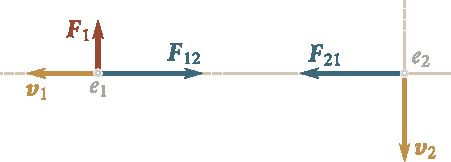
\includegraphics[scale=1]{figures/ch_02/fig_2_1.pdf}
		\caption[]{}
		\label{fig:2_1}
	\end{center}
\end{figure}

Định luật Newton thứ ba khẳng định rằng \textit{các lực mà các vật có tương tác tác dụng lẫn nhau sẽ bằng nhau về độ lớn và ngược chiều nhau}. Dùng các ký hiệu đã nêu ở trên về các lực, nội dung của định luật thứ ba có thể biểu diễn dưới dạng đẳng thức:
\begin{equation}\label{eq:2_17}
\vec{F}_{12} = - \vec{F}_{21}.
\end{equation}

Từ định luật Newton thứ ba suy ra rằng các lực xuất hiện từng cặp: có thể so sánh một lực bất kỳ đặt vào một vật nào đó với một lực bằng nó về độ lớn và ngược chiều đặt vào một vật khác tương tác với vật đã cho.

Định luật Newton thứ ba không phải bao giờ cũng đúng, Nó được nghiệm đúng một cách hoàn toàn nghiêm ngặt trong trường hợp các tương tác tiếp xúc (tức là các tương tác được quan sát khi các vật tiếp xúc trực tiếp) cũng như khi các tương tác của các vật đứng yen nằm cách nhau một khoảng nào đó.

Để làm ví dụ về sự vi phạm định luật Newton thứ ba, có thể dùng một hệ gòm hai hạt mang điện $e_1$ và $e_2$ chuyển động trong lúc khảo sát, như đã chỉ trên \fig{2_1}. Trong điện động lực học người ta đã chứng minh rằng, ngoài lực tương tác tĩnh điện $\vec{F}_{12}$ tuân theo định luật thứ ba còn có lực từ $\vec{F}_1$ tác dụng lên hạt thứ nhất. Còn trên hạt thứ hai chỉ có $\vec{F}_{21}$ bằng $-\vec{F}_{12}$ tác dụng. Độ lớn của lực từ tác dụng lên hạt thứ hai đối với trường hợp đã vẽ trên hình là bằng không. Ta chú ý rằng với các vận tốc của các hạt nhỏ hơn vận tốc ánh sáng trong chân không rất nhiều (với $v_1\ll c$ và $v_2\ll c$) lực $\vec{F}_1$ là nhỏ không đáng kể so với lực $\vec{F}_{12}$, cho nên định luật Newton thứ ba trên thực tế là đúng cả trong trường hợp này.

Bây giờ ta hãy xét một hệ gồm hai hạt $m_1$ và $m_2$ trung hòa về điện, cách xa nhau một khoảng  $r$. Do sự hấp dẫn vũ trụ, các hạt này hút nhau với một lực 
\vspace*{2pt}
\begin{equation}\label{eq:2_18}
F = G\frac{m_1 m_2}{r^2}.
\end{equation}

\noindent
Trong trường hợp này sự tương tác của các hạt được thực hiện thông qua trường hấp dẫn. Ta nói là hạt thứ nhất gây ra trong không gian xung quanh nó một trường mà trường này thể hiện ra ở chỗ là lực hút về hạt thứ nhất tác dụng lên hạt $m_2$ đặt tại một điểm nào đó của trường này. Một cách tương tự, hạt thứ hai gây ra một trường mà nó thể hiện ra ở sự tác dụng lên hạt thứ nhất. Thí nghiệm cho rằng các sự biến đổi của trường được gây ra chẳng hạn bởi sự thay đổi vị trí của hạt gây ra trường lan truyền trong không gian không tức thời với một vận tốc mặc dù rất lớn, nhưng hữu hạn, bằng vận tốc ánh sáng $c$ trong chân không.

\begin{figure}[!htb]
	\begin{center}
		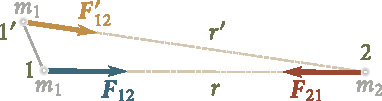
\includegraphics[scale=1]{figures/ch_02/fig_2_2.pdf}
		\caption[]{}
		\label{fig:2_2}
	\end{center}
\end{figure}

Ta hãy giả thử rằng lúc đầu các hạt $m_1$ và $m_2$ đứng yên tại các vị trí $1$ và $2$ (\fig{2_2}). Các lực tương tác $\vec{F}_{12}$ và $\vec{F}_{21}$ bằng nhau về độ lớn và ngược chiều nhau. Bây giờ giả thử hạt $m_1$ dịch chuyển rất nhanh (với vận tốc gần bằng $c$) tới vị trí $1'$. Tại điểm này trên hạt $m_1$ sẽ chịu tác dụng một lực $\vec{F}_{12}'$ nhỏ hơn về độ lớn ($r'>r$) và khác hướng so với $\vec{F}_{12}$ (ta hãy nhớ rằng trường của hạt $m_2$ vẫn không đổi). Còn lực $\vec{F}_{21}$ sẽ tiếp tục tác dụng lên hạt thứ hai, chừng nào mà sự nhiễu loạn của trường gây ra bởi sự dịch chuyển $m_1$ chưa đạt tới điểm $2$. Do đó chừng nào mà hạt $m_1$ đã chuyển động và trong suốt thời gian nào đó sau khi nó đã dừng lại ở điểm $1'$ thì định luật Newton thứ ba đã bị vi phạm.

Nếu hạt $m_1$ dịch chuyển từ điểm $1$ tới điểm $1'$ với vận tốc $v$ nhỏ hơn $c$ nhiều ($v\ll c$) và vận tốc truyền nhiễu loạn của trường đã lớn vô hạn thì các giá trị tức thời của trường ở điểm $2$ đã có thể đáp ứng cho các vị trí của hạt $m_1$ tại cùng thời điểm đó và do đó sự vi phạm định luật thứ ba đã không bị phát hiện.

Cơ học Newton nói chung chỉ đúng đối với các vận tốc chuyển động nhỏ hơn vận tốc ánh sáng nhiều (khi $v\ll c$). Do đó trong phạm vi của môn cơ học này vận tốc truyền nhiễu loạn của trường được coi là vô hạn, nên định luật Newton thứ ba luôn luôn được nghiệm đúng.

\section{Nguyên lý tương đối Galileo}\label{sec:2_7}

Ta hãy nghiên cứu hai hệ qui chiếu chuyển động đối với nhau với vận tốc không đổi $\vec{v}_0$. Một trong những hệ này được ký hiệu trên \fig{2_3} bằng chữ K, ta hãy coi nó một cách quy ước là hệ không chuyển động. Khi đó hệ thứ hai K$'$ sẽ chuyển động thẳng và đều. Ta hãy chọn các trục tọa độ $x, y, z$ của hệ K và các trục $x',y',z'$ của hệ K$'$ sao cho các trục x và $x'$ trùng nhau, còn các trục $y$ và $y'$ cũng như $z$ và $z'$ là song song với nhau.

\begin{figure}[!htb]
	\begin{center}
		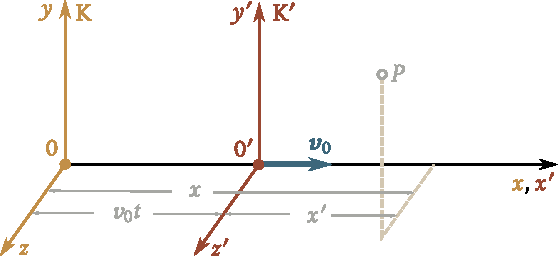
\includegraphics[scale=1]{figures/ch_02/fig_2_3.pdf}
		\caption[]{}
		\label{fig:2_3}
	\end{center}
\end{figure}

Ta hãy tìm sự liên hệ giữa các tọa độ $x, y, z$ của một điểm P nào đó trong hệ K và các tọa độ $x', y', z'$ cũng như điểm đó trong hệ K$'$. Nếu bắt đầu tính thời gian từ lúc mà các gốc tọa độ của hai hệ trùng nhau thì như suy ra từ \fig{2_3}, $x=x'+v_0t$. Ngoài ra, rõ ràng rằng $y=y'$ và $z=z'$. Sau khi đã bổ sung cho các hệ thức này một giả thuyết được thừa nhận trong cơ học cổ điển là thời gian trong cả hai hệ trôi như nhau, nghĩa là $t=t'$, ta được một tập hợp bốn phương trình
\begin{equation}\label{eq:2_19}
x=x'+v_0t,\quad y=y',\quad z=z',\quad t=t'.
\end{equation}

\noindent
gọi là \textbf{các phép biến đổi Galileo}.

Các hệ thức đầu và cuối của \eqref{eq:2_19} chỉ đúng với các giá trị $v_0$ nhỏ so với vận tốc ánh sáng trong chân không mà ta sẽ ký hiệu bằng chữ c $c$ ($v_0\ll c$). Khi $v_0$ vào cỡ $c$ các phép biến đổi Galileo phải được thay thế bằng các phép biến đổi Lorentz tổng quát hơn (xem Sec.~\ref{sec:8_2}). Trong phạm vi cơ học Newton, các công thức \eqref{eq:2_19} được coi là chính xác.

Lấy vi phân các hệ thức \eqref{eq:2_19} theo thời gian, ta hãy tìm sự liên hệ giữa các vận tốc của điểm P đối với các hệ quy chiếu K và K$'$:
\begin{align}
\dot{x} &= \dot{x}'+v_0, \quad\,\,\text{or}\quad\quad v_x=v_x'+v_0\nonumber\\
\dot{y} &= \dot{y}', \quad\quad\,\,\,\,\,\,\,\text{or}\quad\quad v_y=v_y'\label{eq:2_20}\\
\dot{z} &= \dot{z}', \quad\quad\,\,\,\,\,\,\,\,\text{or}\quad\quad v_z=v_z'.\nonumber
\end{align}

Ba hệ thức vô hướng \eqn{2_20} tương đương với hệ thức sau đây giữa vector vận tốc $\vec{v}$ đối với hệ K và vector vận tốc $\vec{v}'$ đối với hệ K$'$:
\begin{equation}\label{eq:2_21}
\vec{v} = \vec{v}' + \vec{v}_0.
\end{equation}

\noindent
Để thấy rõ điều này chỉ cần chiếu đẳng thức vector \eqref{eq:2_21} lên các trục $x, y, z$ là đủ. Kết quả là nguời ta được các công thức \eqref{eq:2_20}.

Các công thức \eqref{eq:2_20} và \eqref{eq:2_21} cho quy tắc cộng các vận tốc trong cơ học cổ điển. Cần để ý rằng hệ thức \eqn{2_21} cũng như mọi hệ thúc vector khác vẫn đúng khi chọn tùy ý các hướng tương hỗ của các trục tọa độ của các hệ K và K$'$. Còn các hệ thức \eqref{eq:2_20}, chỉ đúng khi chọn các trục đã chỉ trên \fig{2_3}.

Trong \ref{sec:2_2} ta đã chú ý rằng một hệ quy chiếu bất kỳ chuyển động đối với một hệ quán tính nào đó với vận tốc không đổi cũng sẽ là hệ quán tính. Bây giờ ta có khả năng chứng minh điều khẳng định này. Muốn vậy ta hãy lấy vi phân theo thời gian \eqn{2_21}. Nếu để ý rằng $\vec{v}_0$ là không đổi ta có
\begin{equation}\label{eq:2_22}
\dot{\vec{v}} = \dot{\vec{v}}', \quad\text{or}\quad  \vec{a} = \vec{a}'.
\end{equation}

\noindent
Từ đây suy ra rằng gia tốc của một vật bất kỳ, trong mọi hệ quy chiếu chuyển động thẳng và đều đối với nhau, là như nhau. Do đó nếu một trong những hệ này là hệ quán tính (điều này có nghĩa là khi không có các lực thì $\vec{a}=0$), thì các hệ còn lại cũng sẽ là các hệ quán tính ($\vec{a}'$ cũng bằng không).

Phương trình cơ bản của cơ học \eqref{eq:2_21} được đặc trưng bởi điều là, trong những đại lượng động học, nó chỉ chứa gia tốc, còn vạn tốc không tham gia vào trong đó. Tuy nhiên, như ta đã thiết lập ở trên, gia tốc của một vật bất kỳ trong hai hệ quy chiếu quán tính chọn tùy ý K và K$'$ là như nhau. Từ đó theo định luật Newton thứ hai suy ra rằng các lực tác dụng lên vật trong các hệ K và K$'$ cũng sẽ như nhau. Do đó, \textit{các phương trình động lực học không biến đổi khi chuyển từ hệ quy chiếu quán tính này sang hệ quy chiếu quán tính khác}, nghĩa là như người ta nói, là bất biến đổi đối với phép biến đổi tọa độ ứng với sự chuyển từ hệ quy chiếu quán tính này sang hệ quy chiếu quán tính khác. Theo quan điểm cơ học tất cả các hệ quy chiếu quán tính là hoàn toàn tương đương nhau: không nên ưu tiên hệ này hơn các hệ khác. Trong thực tế điều này thể hiện ở chỗ là không thể phát hiện hệ ở trạng thái nghỉ hay trạng thái chuyển động đều và thẳng bằng các thí nghiệm cơ học nào đã được biết trong phạm vi của hệ quy chiếu đã cho. Chẳng hạn, khi ngồi trong một toa tàu hỏa chuyển động thẳng và đều, không rung, và không nhìn qua cửa sổ ta không thể xác định được toa tàu chuyển động hay đứng yên. Sự rơi tự do của các vật, sự chuyển động của các vật do ta ném và mọi quá trình cơ học khác trong trường hợp này sẽ xảy ra như trong trường hợp nếu toa tàu không chuyển động.

Những sự kiện đã nêu còn được Galileo Galilei làm sáng tỏ. Luận điểm có nội dung là mọi hiện tượng cơ học trong những hệ quy chiếu quán tính khác nhau đều xảy ra một cách giống nhau, do đó không thể phát hiện được một hệ quy chiếu đã cho là đứng yên hay chuyển động thẳng và đều bằng các thí nghiệm cơ học nào, được gọi là \textbf{nguyên lý tương đối Galileo}.

\section{Các lực}\label{sec:2_8}

Trong vật lý hiện đại người ta phân biệt bốn dạng tương tác: (1) tương tác hấp dẫn (hoặc tương tác gây bởi sự hấp dẫn của vạn vật), (2) tương tác điện từ (được thực hiện thông qua các điện trường và từ trường), (3) tương tác mạnh hoặc tương tác hạt nhân (bảo đảm cho sự liên kết của các hạt trong hạt nhân nguyên tử), và (4) tương tác yếu (rất quan trọng trong nhiều quá trình phân rã các hạt cơ bản).

Trong phạm vi của cơ học cổ điển người ta đề cập đến các lực hấp dẫn và các lực điện từ cũng như các lực đàn hồi và các lực ma sát. Hai dạng lực cuối này được xác định bằng đặc trưng tương tác giữa các phân tử của các chất. Các lực tương tác giữa các phân tử có nguồn gốc điện từ. Do đó các lực đàn hồi và các lực ma sát về bản chất là các lực điện từ.

Các lực hấp dẫn và các lực điện từ là các lực cơ bản, không được quy chúng về các lực khác đơn giản hơn. Còn các lực đàn hồi và các lực ma sát không phải là các lực cơ bản.

Các định luật về các lực cơ bản là đặc biệt đơn giản. Độ lớn của lực hấp dẫn được xác định bằng \eqn{2_18}. Độ lớn của lực mà hai điện tích điểm đứng yên $q_1$ và $q_2$ tương tác với nhau được cho bởi định luật Coulomb:
\vspace{-12pt}
\begin{equation}\label{eq:2_23}
F = k\frac{q_1q_2}{r^2}
\end{equation}

\noindent
($k$ là hệ số tỷ lệ phụ thuộc vào việc chọn các đơn vị tham gia vào công thức của các đại lượng).

Nếu các điện tích chuyển động thì ngoài các lực \eqn{2_23} còn có các lực từ tác dụng lên chúng. Lực từ tác dụng lên một điện tích điểm $q$ chuyển động với vận tốc $\vec{v}$ trong từ trường có cảm ứng từ $\vec{B}$ được xác định bằng công thức
\begin{equation}\label{eq:2_24}
\vec{F} = k'q\,(\vecprod{v}{B})
\end{equation}

\noindent
($k'$ là hệ số tỷ lệ).

Các công thức \eqref{eq:2_18}, \eqref{eq:2_23} và \eqref{eq:2_24} là chính xác. Đối với các lực đàn hồi và các lực ma sát có thể chỉ thu được các công thức thực nghiệm gần đúng mà chúng ta sẽ nghiên cứu trong các mục sau.

\section{Các lực đàn hồi}\label{sec:2_9}

Dưới tác dụng của những lực đặt lên nó, mọi vật thực sẽ bị biến dạng, nghĩa là biến đổi kích thước và hình dạng của mình. Nếu sau khi ngừng tác dụng các lực, vật lại nhận các kích thước và hình dạng ban đầu thì sự biến dạng được gọi là \textbf{sự biến dạng đàn hồi}. Các biến dạng đàn hồi được quan sát trong trường hợp nếu lực gây ra biến dạng không vượt quá một giới hạn nào đó (giới hạn đàn hổi) được xác định cho mỗi vật cụ thể.

\begin{figure}[!htb]
	\begin{center}
		
\includegraphics[scale=1]{figures/ch_02/fig_2_4.pdf}
		\caption[]{}
		\label{fig:2_4}
	\end{center}
\end{figure}

Ta hãy lấy một lò xo có độ dài $l_0$ ở trạng thái không biến dạng và đặt ở đầu lò xo những lực $\vec{F}_1$ và $\vec{F}_2$ bằng nhau về độ lớn và ngược chiều nhau (\fig{2_4}). Dưới tác dụng của các lực này, lò xo bị kéo căng ra một lương $\Delta l$ nào đó, sau đó sự cân bằng lại xảy ra. Ở trạng thái cân bằng các ngoại lực $\vec{F}_1$ và $\vec{F}_2$ sẽ được cân bằng bởi các lực đàn hồi sinh ra trong lò xo do biến dạng. Thí nghiệm cho rằng, với các biến dạng không lớn độ dãn $\Delta l$ của lò xo tỷ lệ với lực kéo căng: $\Delta l\propto F$ (here $F=F_1=F_2$). Một cách tương ứng, lực đàn hồi tỷ lệ với độ dãn của lò xo:
\begin{equation}\label{eq:2_25}
F = k\,\Delta l.
\end{equation}

\noindent
Hệ số tỷ lệ k được gọi là \textbf{hệ số độ cứng} của lò xo.

Điều khẳng định về sự tỷ lệ giữa lực đàn hồi và sự biến dạng được gọi là \textbf{định luật Hooke}.

Các sự dãn đàn hồi xuất hiện trong mọi lò xo. Một phần bất kỳ của lò xo tác dụng lên một phần khác một lực xác định bằng \eqn{2_25}. Do đó nếu cắt lò xo làm đôi thì sẽ xuất hiện một lực đàn hồi có cùng độ lớn trong mỗi nửa với độ dãn nhỏ hơn hai lần. Từ đó ta kết luận rằng với vật liệu đã cho của lò xò và với các kích thước đã cho của vòng xoắn, độ lớn của lực đàn hồi được xác định không phải bằng độ dãn tuyệt đối $\Delta l$ của lò xo mà bằng độ dãn tỷ đối $\Delta l/l_0$.

Khi nén lò xo, cũng xuất hiện các lực căng đàn hồi nhưng có dấu khác. Ta hãy tổng quát hóa \eqn{2_25} bằng cách sau. Đóng chặt đầu này của lò xo (\fig{2_5}) và sẽ coi độ dãn của lò xo như tọa độ $x$ của đầu kia, tính từ vị trí của nó ứng với lò xo không bị biến dạng\footnote{Trên\fig{2_5}b, độ dài đoạn dịch chuyển của đầu lo xo được ký hiệu là $-x$, đó là độ dài của một đoạn thẳng là một đại lượng dương còn tọa độ $x$ trong trường hợp này là âm.}. Ngoài ra, ta sẽ hiểu $F$ là hình chiếu lên trục $x$ của $\vec{F}_{\text{el}}$. Khi đó có thể viết là
\begin{equation}\label{eq:2_26}
F = -k x
\end{equation}

(từ \fig{2_5} rõ ràng là hình chiếu của lực đàn hồi lên trục $x$ và tọa độ $x$ luôn luôn có các dấu khác nhau).

\begin{figure}[!htb]
	\begin{minipage}[t]{0.5\linewidth}
		\begin{center}
			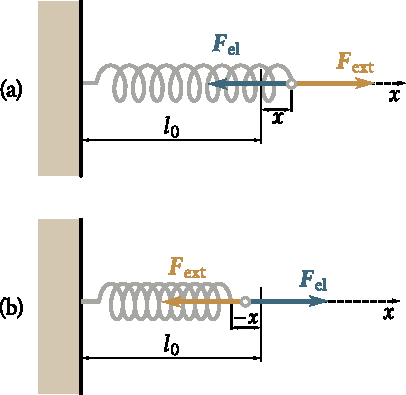
\includegraphics[scale=0.75]{figures/ch_02/fig_2_5.pdf}
			\caption[]{}
			\label{fig:2_5}
		\end{center}
	\end{minipage}
	\hspace{-0.05cm}
	\begin{minipage}[t]{0.5\linewidth}
		\begin{center}
			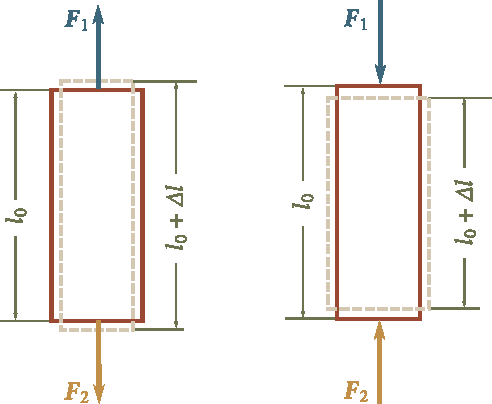
\includegraphics[scale=0.70]{figures/ch_02/fig_2_6.pdf}
			\caption[]{}
			\label{fig:2_6}
		\end{center}
	\end{minipage}
\end{figure}

Các thanh đồng chất có đặc tính giống như lò xo khi dãn hoặc khi nén theo một phía. Nếu tại các đàu của thanh đặt các lực $\vec{F}_1$ và $\vec{F}_2$ ($F_1=F_2=F$) hướng dọc theo trục của nó mà tác dụng của chúng được phân bố đều theo toàn tiết diện, thì độ dài $l_0$ của thanh nhận số gia\footnote{Sự biến đổi độ dài của thanh kéo theo sự biến đổi tương ứng các tiết diện ngang của thanh.} $\Delta l$ dương (khi dãn) hoặc âm (khi nén) (\fig{2_6}). Để làm địa lượng đặc trưng cho sự biến dạng của thanh, người ta lấy một cách tự nhiên độ biến thiên tỷ đối của độ dài của nó:
\begin{equation}\label{eq:2_27}
\varepsilon = \frac{\Delta l}{l_0}.
\end{equation}

Thí nghiệm chứng tỏ rằng đối với các thanh làm bằng vật liệu đã cho độ dãn tỷ đối khi biến dạng đàn hồi tỷ lệ với lực dược tính cho một đơn vị diện tích tiết diện ngang của thanh:
\begin{equation}\label{eq:2_28}
\varepsilon = \alpha\frac{\Delta l}{S}.
\end{equation}

\noindent
($\alpha$ là hệ số tỷ lệ).

Đại lượng bằng tỷ số giữa lực với độ lớn của bề mặt mà trên đó lực tác dụng được gọi là \textbf{ứng suất}. Do tương tác của các phần của vật với nhau, ứng suất được truyền cho tất cả các điểm của vật, nghĩa là toàn bộ thể tích của thanh ở trong trạng thái chịu ứng lực. Nếu lực hướng theo pháp tuyến của mặt thì ứng suất được gọi là \textbf{ứng suất pháp tuyến}. Nếu lực hướng theo tiếp tuyến với mặt mà nó tác dụng thì ứng suất được gọi là \textbf{ứng suất tiếp tuyến}. Ứng suất pháp tuyến thường được ký hiệu bằng chữ $\sigma$, ứng suất tiếp tuyến bằng chữ $\tau$.

Tỷ số $F/S$ trong \eqn{2_28} là ứng suất pháp tuyến $\sigma$. Do đó có thể cho công thức này dạng:
\begin{equation}\label{eq:2_29}
\varepsilon = \alpha\sigma.
\end{equation}

\noindent
Để đặc trưng cho các tính chất đàn hồi của vật liệu người ta dùng đại lượng $E=1/\alpha$ được gọi là \textbf{suất Young. Đại lượng này được đo bằng pascal} ($\SI{1}{\pascal}=\SI{1}{\newton\per\square\metre}$).

Thay thế $\alpha$ trong \eqn{2_9} bằng $1/E$, ta có được hệ thức:
\begin{equation}\label{eq:2_30}
\varepsilon = \frac{\alpha}{E}
\end{equation}

\noindent
từ đó suy ra rằng suất Young sẽ bằng ứng suất pháp tuyến khi độ dãn tỷ đối đã bằng đơn vị (tức là số gia của độ dài $\Delta l$ đã bằng độ dài $l_0$ ban đầu), nếu các biến dạng đàn hồi hết sức lớn đã xảy ra (trong thực tế sự phá hủy thanh xảy ra với các ứng suất nhỏ hơn rất nhiều nên giới hạn đàn đồi đã đạt được sớm hơn).

Giải \eqn{2_28} đối với $F$ và thay thế $\varepsilon$ bằng $\Delta l/l_0$ còn $\alpha$ bằng $1/E$ ta được công thức
\begin{equation}\label{eq:2_31}
F = \frac{E\,S}{l_0}\Delta l = k\,\Delta l
\end{equation}

\noindent
trong đó $k$ là hệ số không đôi đối với thanh đã cho. Hệ thức \eqref{eq:2_31} biểu thị định luật Hooke cho một thanh [so sánh với \eqn{2_26}]. Ta nhớ rằng định luật này chỉ nghiệm đúng khi giới hạn đàn hồi chưa đạt được

\begin{figure}[!htb]
	\begin{center}
		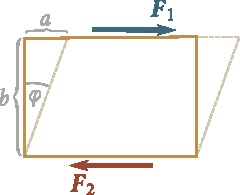
\includegraphics[scale=1]{figures/ch_02/fig_2_7.pdf}
		\caption[]{}
		\label{fig:2_7}
	\end{center}
\end{figure}

Cuối cùng ta hãy nghiên cứu ngắn gọn sự biến dạng dịch. Lấy một vật đồng chất có dạng hình hộp chữ nhật và đặt vào các mặt đối diện của nó các lực $\vec{F}_1$ và $\vec{F}_2$ ($F_1=F_2=F$) hướng song song với các mặt này (~\fig{2_7}). Nếu tác dụng của các lực được phân bố đều theo tất cả bề mặt của mặt tương ứng thì tại một tiết diện bất kỳ song song với các mặt này sẽ xuất hiện một ứng suất tiếp tuyến
\begin{equation}\label{eq:2_32}
\tau = \frac{F}{S}
\end{equation}

\noindent
($S$ là diện tích của mặt). Dưới tác dụng của ứng suất vật bị biến sạng sao cho mặt này bị dịch đối với mặt kia một khoảng $a$ nào đó. Nếu chia vật một cách tưởng tượng thành các lớp mỏng song song với các mặt được khảo sát thì mỗi lớp được dịch đi so với các lớp ở bên cạnh nó. Do nguyên nhân này sự biến dạng có dạng như thế được gọi là \textbf{sự biến dạng dịch}.

Với biến dạng dịch một đường thẳng bất kỳ lúc đầu vuông góc với các lớp sẽ quay đi một góc $\varphi$ nào đó. Để đặc trưng cho biến dạng dịch người ta lấy đại lượng
\begin{equation}\label{eq:2_33}
\gamma = \frac{a}{b} = \tan\varphi
\end{equation}

\noindent
được gọi là \textbf{độ dịch tỷ đối} (ý nghĩa của địa lượng $a$ và $b$ được minh họa trên \fig{2_7}). Với các biến dạng đàn hồi, góc $\varphi$ là rất nhỏ. Vì vật có thể đặt $\tan\varphi\approx\varphi$. Do đó độ dịch tỷ đối bằng góc dịch $\varphi$.

Thí nghiệm chứng tỏ rằng độ dịch tỷ đối tỷ lệ với ứng suất tiếp tuyến
\vspace{-12pt}
\begin{equation}\label{eq:2_34}
\gamma = \frac{1}{G}\tau.
\end{equation}

\noindent
Hệ số $G$ chỉ phụ thuộc vào các tính chất của vật liệu và được gọi là \textbf{suất trượt}. Nó sẽ bằng ứng suất tiếp tuyến khi góc dịch bằng 45 độ ($\tan\varphi=1$), nếu như các biến dạng rất lớn giới hạn đàn hồi đã không bị vượt quá. $G$ và cả $E$ đều được đo bằng (\si{\pascal}).

\section{Các lực ma sát}\label{sec:2_10}

Các lực ma sát xuất hiện trong sự dịch chuyển các vật tiếp xúc với nhau hoặc các phần của chúng đối với nhau. Sự ma sát sinh ra trong sự dịch chuyển tương đối giữa hai vật tiếp xúc với nhau được gọi là \textbf{sự ma sát ngoài}; sự ma sát giữa các phần của cùng một vật liên tục (chẳng hạn, của chất lỏng hoặc chất khí) được gọi là \textbf{sự ma sát trong}.

Cần phải xếp lực ma sát xuất hiện khi một vật rắn chuyển động trong môi trường lỏng hay khí vào loại các lực nội ma sát, vì trong trường hợp này các lớp môi trường trực tiếp tiếp xúc với vật bị lôi kéo vào chuyển động với cùng một vận tốc mà vật có, và sự ma sát giã các lớp này và các lớp môi trường ở bên ngoài đối với chúng sẽ ảnh hưởng tới sự chuyển động của vật.

Sự ma sát giữa các bề mặt của hai vật rắn khi không có một lớp giữa nào đó, chẳng hạn không có sự bôi trơn giữa chúng, được gọi là \textbf{sự ma sát khô}. Sự ma sát giữa một vật rắn và một môi trường lỏng hay khí, cũng như giữa các lớp của môi trường đó được gọi là \textbf{sự ma sát nhớt} (hoặc \textbf{sự ma sát lỏng}).

Đối với sự ma sát khô người ta phân biệt: \textbf{sự ma sát trượt} và \textbf{sự ma sát lăn}.

Các lực ma sát hướng theo tiếp tuyến các mặt trượt (hoặc các lớp), đồng thời sao cho chúng chống lại sự dịch chuyển tương đối của các mặt (các lớp) này. Chẳng hạn, nếu hai lớp chất lỏng trượt lên nhau, chuyển động với vận tốc khác nhau thì lực đặt vào lớp chuyển động nhanh hơn hướng về phía ngược với chuyển động, còn lực tác dụng lên lớp cuyển động chậm hơn hướng về phía chuyển động của lớp này.

\begin{figure}[!htb]
	\begin{center}
		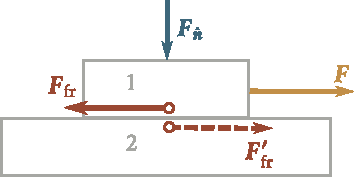
\includegraphics[scale=1]{figures/ch_02/fig_2_8.pdf}
		\caption[]{}
		\label{fig:2_8}
	\end{center}
\end{figure}

\textbf{Sự ma sát khô.} Trong trường hợp ma sát khô lực ma sát xuất hiện không chỉ khi một mặt này trượt trên mặt kia mà cũng cả khi định gây ra sự trượt như thế. Ta hãy xét hai vật $1$ và $2$ tiếp xúc nhau trong đó vật $2$ cố định (\fig{2_8}). Vật $1$ được ép vào vật $2$ bằng lực $\vec{F}_{\hatvec{n}}$ hướng theo pháp tuyến của mặt tiếp xúc của các vật. Nó được gọi là \textbf{áp lực pháp tuyến} và có thể được gây bởi trọng lượng của vật hoặc bởi các nguyên nhân khác. Ta thử dịch chuyển vật $1$ bằng cách tác dụng lên vật một ngoại lực $\vec{F}$. Khi đó người ta phát hiện rằng đối với mỗi cặp vật cụ thể và mỗi giá trị của áp lực pháp tuyến có một giá trị cực tiểu xác định $F_0$ của lực $\vec{F}$ làm cho vật $1$ chuyển dịch được. Với các giá trị của ngoại lực nằm trong các giới hạn từ $0$ đến $F_0$, vật vẫn còn đứng yên. Theo định luật Newton thứ hai, điều này có thể xảy ra trong trường hợp nếu lực $\vec{F}$ được cân bằng với một lực bằng nó về độ lớn nhưng ngược chiều; lực này là lực ma sát nghỉ $\vec{F}_{\text{fr}}$ (xem~\fig{2_8}). Nó tự động\footnote{Điều này xảy ra tương tự như dưới tác dụng của các lực kéo, một lò xo tự động có một độ dãn mà với độ dãn này lực đàn hồi cân bằng với ngoại lực.} nhận giá trị bằng độ lớn $F$ (với điều kiện là lực này không vượt quá $F_0$). Đại lượng $F_0$ là giá trị lớn nhất của lực ma sát nghỉ.

Ta hãy chú ý rằng ứng với định luật Newton thứ ba trên vật $2$ cũng có lực ma sát nghỉ $\vec{F}_{\text{fr}}'$ (trên \fig{2_8}) nó được vẽ bằng đường chấm chấm), bằng lực $\vec{F}_{\text{fr}}$ về độ lớn nhưng có chiều ngược với nó.

Nếu ngoại lực $\vec{F}$ trội hơn $F_0$ về module, thì vật bắt đầu trượt đồng thời gia tốc của vật được xác định bằng hợp lực của hai lực: ngoại lực $\vec{F}$ và lực ma sát nghỉ $\vec{F}_{\text{fr}}$, có độ lớn ở mức nào đó phụ thuộc vào vận tốc trượt. Đặc trưng của sự phục thuộc này được xác định bằng bản chất và trạng thái của các bề mặt trượt. Dạng phụ thuộc của lực ma sát vào vận tốc thường gặp nhất được trình bày trên \fig{2_9}. Đồ thị bao gồm cả trường hợp nghỉ và cả trường hợp trượt. Lực ma sát nghỉ, như đã chỉ rõ, có thể có giát rị từ $0$ đến $F_0$ và được phản ahr trên đồ thị bằng đonạ thẳng đứng. Theo \fig{2_9}, với sự tăng của vận tốc, lực ma sát trượt lúc đầu giảm đi một ít và sau đó lại bắt đầu tăng.
Với sự gia công đặc biệt các mặt tiếp xúc với nhau lực ma sát trượt trên thực tế có thể không phụ thuộc vào vận tốc. Trong trường hợp này phần cong của đọ thi trên \fig{2_9} trở thành đoạn thẳng nằm ngang bắt đầu tại điểm $F_0$.

\begin{figure}[!htb]
	\begin{center}
		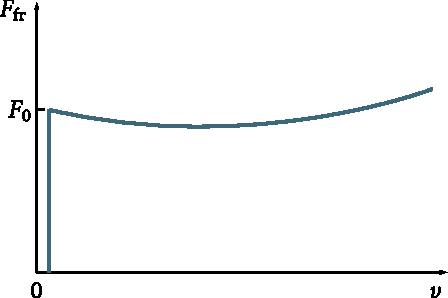
\includegraphics[scale=0.98]{figures/ch_02/fig_2_9.pdf}
		\caption[]{}
		\label{fig:2_9}
	\end{center}
\end{figure}

Các định luật về ma sát khô được quy lại như sau: lực ma sát nghỉ cực đại, cũng như lực ma sát trượt, không phụ thuộc vào diện tích tiếp xúc của các vật trượt và tỷ lệ gần đúng với độ lớn của áp lực pháp tuyến ép các mặt trượt với nhau:
\begin{equation}\label{eq:2_35}
F_{\text{fr}} = f\,F_{\hatvec{n}}.
\end{equation}

\noindent
Hệ số tỷ lệ $f$ không có thú nguyên được gọi là \textbf{hệ số ma sát trượt} (ứng với ma sát nghỉ hay ma sát trượt). Nó phụ thuộc vào bản chất và trạng thái của các mặt trượt, đặc biệt vào độ nhám của chúng. Trong trường hợp trượt, hệ số ma sát là hàm của vận tốc.

Các lực ma sát đóng vai trò rất lớn trong tự nhiên. Trong đời sống hàng ngày của chúng ta sự ma sát luôn luôn có ích. Ta hãy nhớ lại những nỗi khó khăn lớn mà những người đi bộ và các phương tiện vận tải phải trải qua trong thời gian băng phủ mặt đường, khi mà sự ma sát giữa chất phủ lên mặt đường và các đế giày của những người đi bộ hoặc các bánh xe của phương tiện vận tải bị giảm đáng kể. Không có các lực ma sát, thì như trên tàu thủy trong lúc chòng chành, đồ gỗ cần phải gắn chặt vào sàn vì với sự không nằm ngang nhỏ nhất của sàn, nó tụt theo hướng dốc thoai thoải. Bạn đọc có thể tự tìm các vị dú tương tự

Trong nhiều trường hợp vai trò của lực ma sát rất có hại, và cần phải áp dụng biện pháp làm yếu nó tới mức có thể được. Chẳng hạn, tình hình xyar ra với sự ma sát ở trong các ổ bi hoặc có sự ma sát giữa ô trục của bánh xe và trục.

Cách làm giảm cơ bản nhất các lực ma sát là thay thế ma sát trượt bằng sự ma sát lăn, xuất hiện, chẳng hạn, giữa một vật hình trụ hoặc hình cầu và một mặt cong theo đó vật lăn. Sự ma sát lăn về hình thức tuân theo cùng các quy luật như sự ma sát trượt nhưng hệ số ma sát trong trường hợp này là rất nhỏ.

\textbf{Sự ma sát nhớt và sự cản trở của môi trường.} Khác với sự ma sát khô, sự ma sát nhớt được đặc trưng bởi điều là lực ma sát nhớt triệt tiêu đồng thời với vận tốc. Do đó một ngoại lực nhỏ như thế nào đi nữa cũng có thể tăng thêm vận tốc tương đối cho các lớp của môi trường nhớt. Các định luật mà lực ma sát giữa các lớp của môi trường phải tuân theo sẽ được nghiên cứu trong chương dành cho cơ học các chất lỏng.

\begin{figure}[!htb]
	\begin{center}
		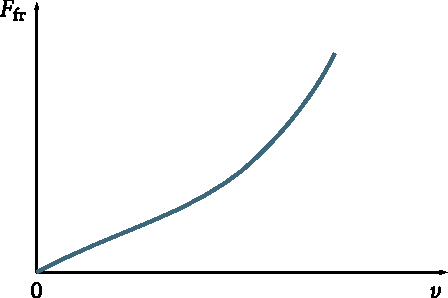
\includegraphics[scale=1]{figures/ch_02/fig_2_10.pdf}
		\caption[]{}
		\label{fig:2_10}
	\end{center}
\end{figure}

Trong tiết này, chúng tôi hạn chế ở việc nghiên cứu các lực ma sát giữa vật rắn và môi trường nhớt (môi trường lỏng hoặc khí). Cần chú ý rằng, thực ra ngoài các lực ma sát, khi các vật chuyển động trong môi trường lỏng hoặc khí, còn xuất hiện các lực cản của môi trường; chúng có thể lớn hơn các lực ma sát rất nhiều. Nếu không có khả năng nghiên cứu tỉ mỉ các nguyên nhân sinh ra các lực này thì ta giới hạn ở sự trình bày các tính quy luật mà các lực ma sát và các lực cản của mô itruowfng cùng tuân theo, đồng thời ta sẽ gọi một cách quy ước lực tổng hợp là lực ma sát. Sự phụ thuộc của các lực này vào vận tốc được trình bày trên \fig{2_10}.

Với các vận tốc không lớn, lực tăng tuyến tính với vận tốc:
\begin{equation}\label{eq:2_36}
\vec{F}_{\text{fr}} = -k_1 \vec{v}
\end{equation}

\noindent
(dấu trừ có nghĩa là lực này hướng ngược chiều với vận tốc). Độ lớn của hệ số $k_1$ phụ thuộc vào dạng và các kích thước của vật, trạng thái bề mặt của nó và vào tính chất của môi trường được gọi là độ nhớt. Chẳng hạn, đối với glycerin hệ số này lớn hơn đối với nước rất nhiều.

Với các vận tốc lớn, định luật tuyến tính chuyển thành định luật bình phương, tức là lực bắt đầu tăng tỷ lệ với bình phương của vận tốc:
\begin{equation}\label{eq:2_37}
\vec{F}_{\text{fr}} = -k_2\, v^2\, \vecuni{v}
\end{equation}

\noindent
($\vecuni{v}$ là chuẩn của vận tốc). Độ lớn của hệ số $k_2$ phụ thuộc vào các kích thước và hình dạng của vật.

Giá trị của vận tốc tại đó định luật \eqref{eq:2_36} chuyển thành \eqref{eq:2_37} sẽ phụ thuộc vào hình dạng và kích thước của vật cũng như phụ thuộc vào các tính chất nhớt và khối lượng riêng của môi trường.

\section{Trọng lực và trọng lượng}\label{sec:2_11}

Dưới tác dụng của lực hút về Trái đất mọi vật rơi với một gia tốc đối với mặt đất được ký hiệu bằng chữ $g$. Điều này có nghĩa là trong hệ quy chiếu gắn với Trái đất, mỗi vật có khối lượng $m$ chịu tác dụng một lực
\begin{equation}\label{eq:2_38}
\vec{P} = m\vec{g}
\end{equation}

\noindent
được gọi là trọng lực\footnote{Do tính không quán tính của hệ quy chiếu gắn với Trái đất, trọng lực khác ít so với lực mà vật bị trái đất hút. Chi tiết về điều này sẽ nói trong \ref{sec:4_2}.}. Khi vật đứng yên đối với mặt đất thì lực $\vec{P}$ được cân bằng bởi phản lực\footnote{Các lực mà các vật tác dụng lên vật đã cho, làm hạn chế sự chuyển động của nó, được gọi là các phản lực.} $\vec{F}_{\text{r}}$ của giá treo hoặc giá đỡ giữ cho vật khỏi rơi ($\vec{F}_{\text{r}}=-\vec{P}$). Theo định luật Newton thứ ba trong trường hợp này vật tác dụng lên giá treo hoặc giá đỡ một lực $\vec{W}$ bằng $-\vec{F}_{\text{r}}$, tức là một lực
\begin{equation*}
\vec{W} = \vec{P} = m\vec{g}
\end{equation*}

\begin{figure}[!htb]
	\begin{center}
		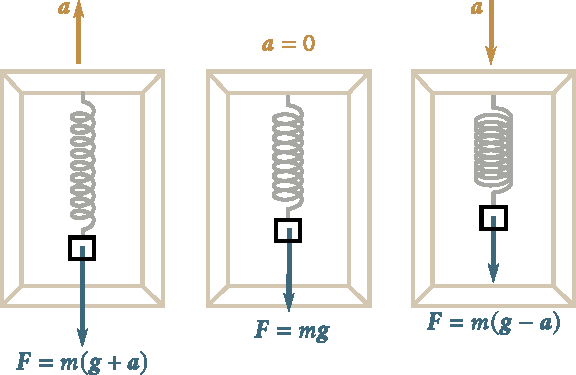
\includegraphics[scale=1]{figures/ch_02/fig_2_11.pdf}
		\caption[]{}
		\label{fig:2_11}
	\end{center}
\end{figure}

Lực $\vec{W}$ mà vật tác dụng lên giá treo hoặc giá đỡ được gọi là \textbf{trọng lượng} của vật. Lực này bằng $m\vec{g}$ chỉ trong trường hợp nếu vật và giá đỡ (hoặc giá treo) không chuyển động đối với Trái đất. Trong trường hợp chúng chuyển động với một gia tốc $\vec{a}$ nào đó, trọng lượng $\vec{W}$ sẽ không bằng $m\vec{g}$. Có thể làm sáng tỏ điều này bằng ví dụ sau đây. Giả thử giá treo là một lò xo được đóng chặt vào một cái khung và chuyển động cùng với vật với gia tốc $\vec{a}$ (\fig{2_11}). Khi đó phương trình chuyển động của vật sẽ có dạng
\begin{equation}\label{eq:2_39}
\vec{P} + \vec{F}_{\text{r}} = m\vec{a}
\end{equation}

\noindent
trong đó $\vec{F}_{\text{r}}$ là phản lực của giá treo, tức là lực mà lò xò tác dụng lên vật. Theo định luật Newton thứ ba vật tác dụng lên lò xo một bằng bằng $-\vec{F}_{\text{r}}$ mà theo định nghĩa là trong lượng $\vec{W}$ của vật trong các điều kiện này. Thay thế phản lực $\vec{F}_{\text{r}}$ trong \eqn{2_39} bằng lực $-\vec{W}$, còn trọng lực $\vec{P}$ bằng tích số $m\vec{g}$, ta được
\begin{equation}\label{eq:2_40}
\vec{W} = m(\vec{g} - \vec{a}).
\end{equation}

\noindent
Công thức \eqref{eq:2_40} xác định trọng lượng của vật trong trường hợp tổng quát. Nó đúng đối với giá treo hoặc giá đỡ có dạng bất kỳ.
Ta giả thử rằng vật và giá treo chuyển động theo hướng thẳng đứng (\fig{2_11} ứng với giả thiết này).

Ta chiếu \eqn{2_40} lên hướng của dây rọi:
\begin{equation}\label{eq:2_41}
W = m(g \pm a).
\end{equation}

\noindent
Trong biểu thức này, $W$, $g$, và $a$ là module của các vector tương ứng. Dấu "+" ứng với a hướng lên trên, dấu "-" ứng với hướng của a xuống dưới.

Từ \eqn{2_41}, suy ra rằng, về module trọng trường $\vec{W}$ có thể lớn hơn hoặc nhỏ hơn trọng lực $\vec{P}$. Khi khung với giá treo rơi tự do thì, $\vec{a}=\vec{g}$, và lực $\vec{W}$ mà vật tác dụng lên giá treo bằng không. Trạng thái không trọng lượng bắt đầu. Con tàu vũ trụ bay xung quanh Trái đất với các động cơ bị tắt sẽ chuyển động như một khung rơi tự do với gia tốc $\vec{g}$, vì vậy các vật trong con tàu ở trạng thái không trọng lượng, nghĩa là chúng không gây áp suất lên các vật tiếp xúc với chúng.

Ta hãy để ý rằng, thường người ta hay nhầm lẫn trọng lực $\vec{P}$ và trọng lượng $\vec{W}$ của vật. Điều này xảy ra là do trong trường hợp giá đỡ không chuyển động các lực $\vec{P}$ và $\vec{P}$ trùng nhau về độ lớn và hướng (cả hai đều bằng $m\vec{g}$). Tuy nhiên cần phải nhớ rằng các lực này được đặt vào các vật khác nhau: $\vec{P}$ được đặt vào chính vật, $\vec{W}$ được đặt vào giá treo hoặc giá đỡ, hạn chế chuyển động tự do của vật trong trường lực hút của Trái đất. Ngoài ra, lực $\vec{P}$ luôn luôn bằng $m\vec{g}$, không phụ thuộc vào vật chuyển động hay đứng yên, còn lực của trọng lượng $\vec{W}$ phụ thuộc vào gia tốc của giá đỡ và vật chuyển động, thêm vào đó nó có thể hoặc lớn hơn hoặc nhỏ hơn $m\vec{g}$ và đặc biệt là nó triệt tiêu ở trạng thái không trọng lượng.

Hệ thức \eqref{eq:2_40} giữa khối lượng và trọng lượng của vật cho cách so sánh các khối lượng của các vật bằng cách cân: tỷ số các trọng lượng của các vật được xác định trong những điều kiện giống nhau (thông thường với $\vec{a}=0$) tại cùng một điểm trên mặt đất bằng tỷ số các khối lượng của các vật này:
\begin{equation*}
W_1\,:\,W_2\,:\,W_3\,:\,\ldots = m_1\,:\,m_2\,:\,m_3\ldots.
\end{equation*}

Như sẽ chứng tỏ trong \ref{sec:4_2}, gia tốc rơi tự do $g$ và trọng lực $P$ phụ thuộc vào vĩ độ của khu vực. Ngoài ra, $P$ và $g$ cũng phụ thuộc vào độ cao trên mặt biển - chúng sẽ giảm khi đi ra xa tâm Trái đất.

\section{Ứng dụng thực tế của các định luật Newton}\label{sec:2_12}

\begin{figure}[!htb]
	\begin{center}
		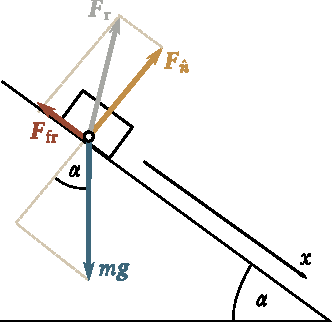
\includegraphics[scale=1]{figures/ch_02/fig_2_12.pdf}
		\caption[]{}
		\label{fig:2_12}
	\end{center}
\end{figure}

Để thành lập phương trình chuyển động trước hết cần phải thiết lập những lực nào tác dụng lên vật đang khảo sát. Đồng thời cần chú ý làm sáng tỏ tác dụng của các vật nào khác lên vật đã cho. Chẳng hạn đối với vật trượt trên mặt phẳng nghiêng (\fig{2_12}), thì tác động từ phía Trái đất (được đặc trưng bằng lực $m\vec{g}$) và tác động từ phía mặt phẳng (được đặc trưng bằng phản lực $\vec{F}_{\text{r}}$) là chủ yếu.

Hoàn toàn không cần đưa vào sự khảo sát các lực ``chuyển động'', ``lăn'', ``hướng tâm'', ``ly tâm''\footnote{Điều này không liên quan tới thuật ngữ ``lực quán tính ly tâm'' (xem Sec.~\ref{sec:4_2}.} và các lực tương tự như thế. Để tránh sai lầm cần phải đặc trưng các lực không theo tác dụng do chúng gây ra mà theo ``nguồn gốc'' gây ra sự xuất hiện lực. Điều này có nghĩa là ứng với mỗi lực cần phải nhìn thấy vật mà lực được gây ra bởi sự tác động của vật. Khi đó rõ ràng sẽ không thể xảy ra sai sót điển hình là cùng một lực được hai lần tính đến dưới các tên gọi khác nhau.

Trong ví dụ đang xét (xem~\fig{2_12}), một cách hợp lý là chia phản lực $\vec{F}_{\text{r}}$ thành hai phần là lực pháp tuyến $\vec{F}_{\hatvec{n}}$ và lực ma sát $\vec{F}_{\text{fr}}$. Đặc biệt điều này có lợi vì lực ma sát tỷ lệ mới module của lực $\vec{F}_{\hatvec{n}}$ [xem~\eqn{2_35}].

Sau khi xác định các lực tác dụng lên vật người ta thành lập phương trình của định luật Newton thứ hai. Trong ví dụ của ta nó có dạng
\begin{equation}\label{eq:2_42}
m\vec{a} = m\vec{g} + \vec{F}_{\text{r}} = m\vec{g} + \vec{F}_{\hatvec{n}} + \vec{F}_{\text{fr}}.
\end{equation}

\noindent
Để thực hiện các phép tính toán cần phải chuyển từ các vector sang các hình chiếu của chúng lên các hướng đã chọn một cách thích hợp. Đồng thời người ta sử dụng các tính chất sau đây của hình chiếu:
\begin{enumerate}[(1)]
	\item các vector bằng nhau có các hình chiếu như nhau;
	\item hình chiếu của vector mà vector này bằng tích của một vector khác với một vô hướng, sẽ bằng tích hình chiếu của vector thứ hai này với vô hướng đó;
	\item hình chiếu của tổng các vector bằng tổng các hình chiếu của các vector số hạng [xem~\eqn{1_8}].
\end{enumerate}

Ta hãy chiếu các vector tham gia vào \eqn{2_42} lên hướng $x$ đã nêu trên \fig{2_12}. Hình chiếu của các vector bằng $a_x=a$ ($a$ là module của vector $\vec{a}$), $g_x=g\sin\alpha$, $F_{\hatvec{n}x}=0$, $F_{\text{r}x}=-f F_{\hatvec{n}x}=-fmg\cos\alpha$. Do đó ta đi đến phương trình
\begin{equation*}
ma = mg\sin\alpha - fmg\cos\alpha
\end{equation*}

\noindent
mà từ phương trình này dễ dàng tìm được $a$.

Trong các trường hợp phức tạp hơn đành phải chiếu các vector lên một số hướng và giải hệ các phương trình đại số hoặc vi phân thu được.

% \cleardoublepage
% % !TEX root = saveliev_physics_general_course_1.tex
%!TEX TS-program = pdflatex
%!TEX encoding = UTF-8 Unicode


\chapter{CÁC ĐỊNH LUẬT BẢO TOÀN}\label{chap:3}

\section{Các đại lượng được bảo toàn}\label{sec:3_1}

Các vật tạo thành hệ cơ học có thể tương tác với nhau cũng như các vật không phụ thuộc hệ này. Ứng với điều này có thể chia các lực tác dụng lên các vật của hệ thành \textbf{nội lực} và \textbf{ngoại lực} . Ta sẽ gọi các lực mà các vật còn lại của hệ tác động lên vật đã cho là các nội lực, và các lực được gây bởi tác động của các vật không thuộc hệ là các ngoại lực.

Trong trường hợp nếu không có các ngoại lực thì hệ được gọi là \textbf{hệ kín}.

Đối với các hệ kín tồn tại các hàm của các tọa độ và của vận tốc của các hạt tạo thành hệ\footnote{Ta hãy nhớ rằng, để ngắn gọn ta gọi chất điểm là hat.} giữ nguyên giá trị không đổi khi chuyển động. Các hàm này được gọi là các \textbf{tích phân chuyển động}.

Đối với một hệ gồm $N$ hạt mà giữa chúng không có các liên kết rắn thì có thể thành lập được $6N-1$ tích phân chuyển động. Tuy nhiên trong chúng người ta chỉ quan tâm đến các tích phân chuyển động có tính chất cộng tính. Tính chất này có nội dung là giá trị của tích phân chuyển động đối với hệ gồm các hạt mà có thể bỏ qua tương tác của chúng, bằng tổng các giá trị của tích phân chuyển động đối với từng hạt tách biệt. Có ba tích phân chuyển động cộng tính. Một trong chúng được gọi là \textbf{năng lượng}, cái thứ hai là \textbf{xung lượng}, và cái thứ ba là \textbf{momen xung lượng}.

Như vậy đối với các hệ kín có ba đại lượng vật lý không biến đổi (được bảo toàn): năng lượng, xung lượng và momen xung lượng. Ứng với điều này có \textbf{ba định luật bảo toàn}---định luật bảo toàn năng lượng, định luật bảo toàn xung lượng và định luật bảo toàn momen xung lượng. Các định luật này liên hệ chặt chẽ với các tính chất cơ bản của không gian và thời gian.

\textbf{Sự đồng tính của thời gian} là cơ sở của sự bảo toàn năng lượng, nghĩa là tính tương đương của tất cả các thời điểm. Cần hiểu tính tương đương theo nghĩa là sự thay thế thời điểm $t_1$ bằng thời điểm $t_2$ mà không làm biến đổi giá trị của các tọa độ và vận tốc của các hạt thì sẽ không làm biến đổi các tính chất cơ học của hệ. Điều này có nghĩa là sau sự thay thế nói trên các tọa độ và vận tốc của các hạt tại thời điểm $t_2+t$ bất kỳ cũng sẽ có cùng các giá trị mà chúng đã có tại thời điểm $t_1+t$ trước khi thay thế.

\textbf{Sự đồng tính của không gian} là cơ sở của sự bảo toàn xung lượng, nghĩa là sự đồng nhất của các tính chất của không gian tại mọi điểm. Cần phải hiểu sự đồng nhất theo nghĩa là khi dịch chuyển song song một hệ kín từ chỗ này trong không gian sang chỗ kia mà không thay đổi vị trí tương hỗ và các vận tốc của hạt thì sẽ không làm biến đổi các tính chất cơ học của hệ (giả sử rằng ở chỗ mới tính kín của hệ không bị phá hủy). 

Sau cùng, \textbf{tính đẳng hướng của không gian} là cơ sở của sự bảo toàn momen xung lượng, nghĩa là sự đồng nhất của các tính chất của không gian theo mọi hướng. Cần phải hiểu sự đồng nhất theo nghĩa là sự quay một hệ kín hoàn toàn không ảnh hưởng tới các tính chất cơ học của hệ.

Các định luật bảo toàn là một vũ khí rất có hiệu lực của việc nghiên cứu. Thông thường lời giải chính xác của phương trình chuyển động là rất phức tạp. Trong những trường hợp này nhờ các định luật bảo toàn có thể thu được một loạt dữ kiện quan trọng về sự diễn biến của các hiện tượng cơ học mà không phải giải các phương trình chuyển động. Các định luật bảo toàn không phụ thuộc vào đặc tính của các lực tác dụng. Do đó, nhờ chúng có thể thu được một loạt thông tin quan trọng về trạng thái của các hệ cơ học ngay cả trong các trường hợp khi các lực đều chưa biết.

Trong các tiết sau ta sẽ thu được các định luật bảo toàn xuất phát từ các phương trình Newton. Tuy nhiên cần chú ý rằng các định luật bảo toàn có tính tổng quát lớn hơn các định luật Newton rất nhiều. Các định luật bảo toàn thực sự vẫn còn đúng ngay cả khi các định luật Newton (cụ thể là định luật thứ ba) bị vi phạm. Ta hãy nhấn mạnh rằng các định luật bảo toàn năng lương, xung lượng và momen xung lượng là các đinh luật chính xác cũng đúng là một cách nghiêm ngặt cả trong lĩnh vực tương đối tính.

\section{Động năng}\label{sec:3_2}

Ta bắt đầu tìm các tích phân chuyển động cộng tính. Để bắt đầu ta xét hệ đơn giảm gồm một hạt (một chất điểm).

Ta viết phương trình chuyển động của hạt:
\begin{equation}\label{eq:3_1}
m\dot{\vec{v}} = \vec{F}.
\end{equation}

\noindent
Ở đây $\vec{F}$ là lực tổng hợp tác dụng lên hạt. Nhân phương trình~\eqn{3_1} với độ dịch chuyển của hạt $\mathrm{d}\vec{s}=\vec{v}\,\mathrm{d}t$, ta có:
\begin{equation}\label{eq:3_2}
m\vec{v}\dot{\vec{v}}\,\mathrm{d}t = \vec{F}\,\mathrm{d}\vec{s}.
\end{equation}

\noindent
Tích $\dot{\vec{v}}\,\mathrm{d}t$ là số gia $\mathrm{d}\vec{v}$ của vận tốc hạt trong thời gian $\mathrm{d}t$. Một cách tương ứng
\begin{equation}\label{eq:3_3}
m\vec{v}\dot{\vec{v}}\,\mathrm{d}t = m\vec{v}\,\mathrm{d}\vec{v} = m\,\mathrm{d}\!\left(\frac{v^2}{2}\right) = \mathrm{d}\!\left(\frac{mv^2}{2}\right)
\end{equation}

\noindent
%[see \eqn{2_50}].
Nếu thay thế vào \eqn{3_2}, ta đi tới hệ thức
\begin{equation}\label{eq:3_4}
\mathrm{d}\!\left(\frac{mv^2}{2}\right) = \vec{F}\,\mathrm{d}\vec{s}.
\end{equation}

\noindent
Nếu hệ kín, $\vec{F}=0$, thì $\mathrm{d}(mv^2/2)=0$, còn chính đại lượng
\begin{equation}\label{eq:3_5}
E_{\text{k}} = \frac{mv^2}{2}
\end{equation}

\noindent
vẫn không đổi. Đại lượng này được gọi là \textbf{động năng} của hạt. Trong trường hợp một hạt cô lập, động năng là một tích phân chuyển động\footnote{Trong trường hợp một hạt cô lập thì bất kỳ mức nào của vận tốc vẫn không đổi. Tuy nhiên trong trường hợp hệ gồm số hạt tương tác với nhau thì chính các đại lượng có dạng~\eqref{eq:3_5} sẽ tham gia vào các tích phân chuyển động cộng tính như các số hạng. }.

Nhân tử số và mẫu số của biểu thức~\eqref{eq:3_5} với $m$ và để ý rắng tích số $mv$ bằng xung lượng $p$ của vật, có thể cho biểu thức đối với động năng dạng:
\begin{equation}\label{eq:3_6}
E_{\text{k}} = \frac{p^2}{2m}.
\end{equation}

\noindent
Nếu lực $\vec{F}$ tác dụng lên hạt thì động năng sẽ thay đổi. Trong trường hợp này theo~\eqref{eq:3_4} số gia của động năng của hạt trong thời gian $\mathrm{d}\vec{t}$ bằng tích vô hướng $\vec{F}\,\mathrm{d}\vec{s}$ ($\mathrm{d}\vec{s}$ là độ dời của hạt trong thời gian $\mathrm{d}t$). Đại lượng 
\begin{equation}\label{eq:3_7}
\mathrm{d}A = \vec{F}\,\mathrm{d}\vec{s}
\end{equation}

\noindent
được coi là \textbf{công} do lực $\vec{F}$ thực hiện trên quãng đường $\mathrm{d}s$ ($\mathrm{d}s$ là module độ rời $\mathrm{d}\vec{s}$). Có thể biểu diễn tích vô hướng \eqref{eq:3_7} dưới dạng tích của các hình chiếu của lực trên hướng chuyển dời $F_{\text{s}}$ và của yếu tố đường đi $\mathrm{d}s$. Do đó có thể viết là 
\begin{equation}\label{eq:3_8}
\mathrm{d}A = F_{\text{s}}\,\mathrm{d}s.
\end{equation}

\noindent
Từ điều đã nói rõ ràng rằng công đặc trưng cho sự biến đổi năng lượng gây ra bởi tác dụng của lực lên hạt chuyển động.

Ta hãy lấy tích phân hệ thức~\eqref{eq:3_4} dọc theo quỹ một quỹ đạo nào đó từ điểm $1$ đến điểm $2$:
\begin{equation*}
\int_{1}^{2} \mathrm{d}\!\left(\frac{mv^2}{2}\right) = \int_{1}^{2} \vec{F}\,\mathrm{d}\vec{s}.
\end{equation*}

\noindent
Vế trái là hiệu các giá trị của động năng tại các điểm $2$ và $1$, tức là số gia\footnote{Có thể đặc trưng sự biển đổi của đại lượng $a$ nào đó hoặc bằng số gia hoặc bằng độ giảm của nó. Người ta gọi hiệu của giá trị cuối ($a_2$) và giá trị ban đầu ($a_1$) của đại lượng $a$ là số gia của đại lượng này và ta sẽ ký hiệu nó bằng $\Delta a$: 

$\text{số gia}=\Delta a=a_2-a_1$. 

Người ta gọi độ giảm của đại lượng $a$ là hiệu của giá trị ban đầu ($a_1$) và giá trị cuối ($a_2$): 

$\text{độ giảm}=a_1-a_2=-\Delta a$. 

Độ giảm của một đại lượng bằng số gia của nó lấy dấu ngược lại. Số gia và độ giảm là các đại lượng đại số.} của động năng trên quãng đường $1$-$2$. Để ý đến điều đó, ta có:
\begin{equation}\label{eq:3_9}
E_{\text{k},2} - E_{\text{k},1} = \frac{mv^2_2}{2} - \frac{mv^2_1}{2} = \int_{1}^{2} \vec{F}\,\mathrm{d}\vec{s}.
\end{equation}

Đại lượng 
\begin{equation}\label{eq:3_10}
A = \int_{1}^{2} \vec{F}\,\mathrm{d}\vec{s} = \int_{1}^{2} F_{\text{s}}\,\mathrm{d}s
\end{equation}

\noindent
là công của lực $\vec{F}$ trên quãng đường $1$-$2$. Đôi khi ta ký hiệu công này bằng ký hiệu $A_{12}$ thay cho $A$.

Vậy, \textit{công của tất cả các lực tổng hợp tác dụng lên hạt chuyển thành độ tăng động năng của hạt}:
\begin{equation}\label{eq:3_11}
A_{12} = E_{\text{k},2} - E_{\text{k},1}.
\end{equation}

\noindent
Từ \eqn{3_11} suy ra rằng năng lượng có cùng thứ nguyên như công. Ứng với điều này, năng lượng được đo bằng cùng các đơn vị giống như công (xem mục sau).


\section{Công}\label{sec:3_3}

Ta hãy khảo sát đại lượng được gọi là công một cách tỉ mỉ hơn. Có thể biểu diễn biểu thức~\eqref{eq:3_7} dưới dạng
\begin{equation}\label{eq:3_12}
\mathrm{d}A = \vec{F}\,\mathrm{d}\vec{s} = F\cos\alpha\,\deriv{s}
\end{equation}

\noindent
trong đó $\alpha$ là góc giữa hướng của lực và hướng dịch chuyển của điểm đặt lực.

Nếu lực và hướng dịch chuyển tạo thành một góc nhọn  ($\cos\alpha>0$) thì công là dương. Nếu góc $\alpha$ là góc tù ($\cos\alpha<0$) thì công là âm. Với $\alpha=\pi/2$ công bằng không. Điều sau cùng chứng tỏ đặc biệt rõ ràng rằng khái niệm công trong cơ học khác hẳn với khái niệm hàng ngày về công. Trong cách hiểu thông thường, mọi sự nỗ lực, cụ thể là sự căng cơ bắp luôn luôn kèm theo sự thực hiện công. Chẳng hạn, để giữ một vật nặng đứng yên, hơn nữa để dịch chuyển vật này theo quãng đường nằm ngang, người mang sẽ tiêu tốn nhiều sức lực, nghĩa là ``thực hiện công''. Tuy nhiên công như một đại lượng cơ học, trong các trường hợp này là bằng không.

\begin{figure}[!htb]
	\begin{center}
		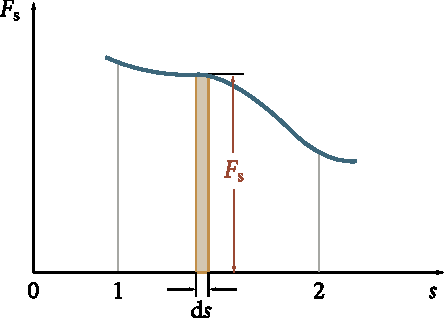
\includegraphics[scale=1]{figures/ch_03/fig_3_1.pdf}
		\caption[]{}
		\label{fig:3_1}
	\end{center}
\end{figure}

Trên hình~\ref{fig:3_1}, trình bày đồ thị hình chiếu  của lực lên hướng dịch chuyển $F_{\text{s}}$ như một hàm của vị trí của hạt trên quỹ đạo (có thể gọi trục hoành là trục $s$, độ dài của đoạn trục này giữa hai điểm $1$ và $2$ bằng độ dài toàn phần của quãng đường). Từ hình vẽ rõ ràng là công nguyên tố $\deriv{A}=F_{\text{s}}\,\deriv{s}$ về trị số bằng diện tích của dải gạch gạch, còn công $A$ trên quãng đường $1$-$2$ về trị số bằng diện tích của hình được được giới hạn bởi đường cong $F_{\text{s}}$, các đường thẳng đứng $1$ và $2$ và trục $s$ (so với \fig{1_26}).

Ta hãy áp dụng kết quả này để tìm công thực hiển trong sự biến dạng của lò xo tuần theo định luật Hooke   (xem \fig{2_5} và công thức \eqref{eq:2_26}). Ta bắt đầu từ sự giãn của lò xo. Ta sẽ thực hiện sự giãn rất chậm để lực $\vec{F}_{\text{ext}}$ mà ta tác dụng lên lò xo có thể luôn luôn được coi bằng lực đàn hồi $\vec{F}_{\text{el}}$ về độ lớn. Khi đó, $\vec{F}_{x,\text{ext}}=-\vec{F}_{x,\text{el}}=kx$, trong đó  $x$ là độ dãn của lò xo (\fig{3_2}). Từ hình vẽ rõ ràng là công cần thực hiện để gây ra độ dãn $x$ của lò xo bằng
\begin{equation}\label{eq:3_13}
A = \frac{kx^2}{2}.
\end{equation}

\noindent
Khi nén lò xo một lượng $x$ thì về độ lớn và về dấu công được thực hiện cũng giống như khi dãn một lượng $x$. Hình chiếu của lực $\vec{F}_{\text{ext}}$ trong trường hợp này là âm ($\vec{F}_{\text{ext}}$ hướng về phía bên trái, $x$ tăng lên về bên phải, xem \fig{3_2}), tất cả $\deriv{x}$ cũng đều âm. Do đó, tích $\vec{F}_{x,\text{ext}}\,\deriv{x}$ là dương.

\begin{figure}[!htb]
	\begin{center}
		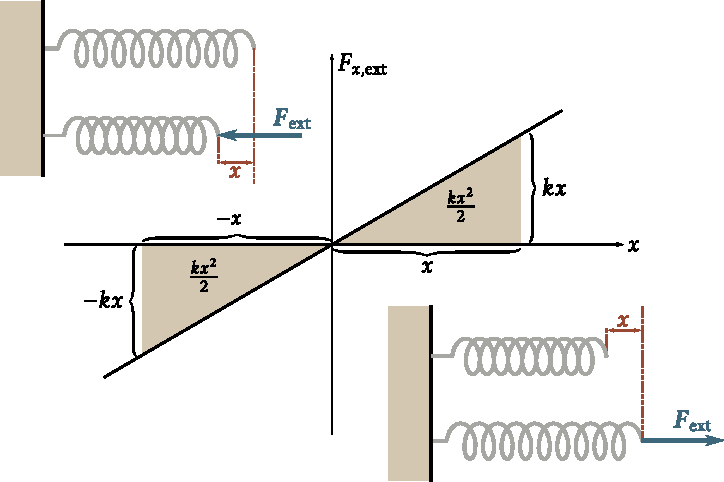
\includegraphics[scale=0.95]{figures/ch_03/fig_3_2.pdf}
		\caption[]{}
		\label{fig:3_2}
	\end{center}
\end{figure}

Một cách tương tự có thể tìm biểu thức đối với công thực hiện khi dãn hoặc nén đàn hồi một thanh. Theo công thức \eqref{eq:2_31}, công này bằng
\begin{equation}\label{eq:3_14}
A = \frac{1}{2}\frac{ES}{l_0}(\Delta l)^2 = \frac{1}{2}ESl_0\left(\frac{\Delta l}{l_0}\right)^2 = \frac{1}{2}EV\varepsilon^2
\end{equation}

\noindent
trong đó $V=Sl_0$ là thể tích của thanh, còn $\varepsilon=\Delta l/l_0$ là độ dãn tỷ đối (xem \eqnref{eq:2_27}).

Giả sử một số lực mà    lực tổng hợp của chúng bằng  $\vec{F}=\sum_{i}\vec{F}_i$ tác dụng đồng thời lên vật. Từ tính phân phối của tích vô hướng của các vector  (xem \eqref{eq:1_20}) suy ra rằng công $\deriv{A}$ thực hiện bởi lực tổng hợp trên quãng đường $\deriv{s}$ có thể được biểu diễn dưới dạng
\begin{equation}\label{eq:3_15}
\deriv{A} = \left(\sum_{i}\vec{F}_i\right)\deriv{s} = \sum_{i}\vec{F}_i\,\deriv{\vec{s}} = \sum_{i}\deriv{A}_i.
\end{equation}

\noindent
Điều này có nghĩa là công của lực tổng hợp của một số lực bằng tổng đại số các công được thực hiện bởi từng lực tách biệt.

Độ dời nguyên tố $\deriv{\vec{s}}$ có thể được biểu diễn như $\vec{v}\deriv{t}$. Do đó có thể cho biểu thức đối với công nguyên tố dạng
\begin{equation}\label{eq:3_16}
\deriv{A} = \vec{F}\vec{v}\,\deriv{t}.
\end{equation}

\noindent
Khi đó thực hiện trong khoảng thời gian $t_1$ đến $t_2$ có thể tính theo công thức
\begin{equation}\label{eq:3_17}
A = \int_{t_1}^{t_2}\vec{F}\,\deriv{t}.
\end{equation}

Ứng với \eqref{eq:1_21} $\vec{F}\,\deriv{\vec{s}}=F\,\deriv{s_F}$, trong đó $\deriv{s_F}$, là hình chiếu của độ dời nguyên tố $\deriv{\vec{s}s}$ lên hướng của lực $\vec{F}$. Do đó có thể viết công thức đối với công như sau:
\begin{equation}\label{eq:3_18}
\deriv{A} = F\,\deriv{s_F}.
\end{equation}

\begin{figure}[!htb]
	\begin{center}
		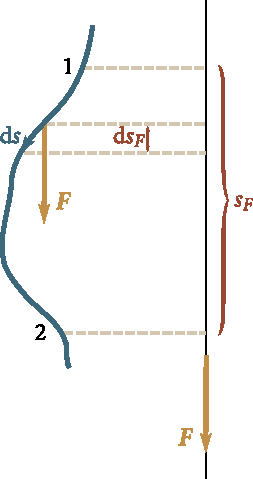
\includegraphics[scale=0.95]{figures/ch_03/fig_3_3.pdf}
		\caption[]{}
		\label{fig:3_3}
	\end{center}
\end{figure}

Nếu lực có độ lớn và hướng không đổi (\fig{3_3}), thì có thể đưa vector $\vec{F}$ trong biểu thức đối với công ra ngoài dấu tích phân, kết quả ta có công thức
\begin{equation}\label{eq:3_19}
A = \vec{F}\int_{1}^{2}\deriv{\vec{v}} = \vecdot{F}{s} = F s_F
\end{equation}

\noindent
trong đó $\vec{s}$ là vector độ dời từ điểm $1$ đến điểm $2$, còn $s_F$ là hình chiếu của nó lên hướng của lực.
Công được thực hiện trong một đơn vị thời gian được gọi là công suất. Nếu công $\deriv{A}$ được thực hiện trong khoảng thời gian $\deriv{t}$ thì công suất bằng
\begin{equation}\label{eq:3_20}
P = \diff{A}{t}.
\end{equation}

\noindent
Nếu lấy $\deriv{A}$ ở dạng \eqref{eq:3_16}, ta được biểu thức đối với công suất 
\begin{equation}\label{eq:3_21}
P = \vecdot{F}{v}
\end{equation}

\noindent
theo biểu thức này công suất bằng tích vô hướng của vector lực với vector vận tốc chuyển động của điểm đặt lực. 

\textbf{Các đơn vị công và công suất.} Để làm đơn vị công người ta dùng công được thực hiện bởi lực bằng một đơn vị và tác dụng theo hướng dịch chuyển bởi lực bằng một đơn vị và tác dụng theo hướng dịch chuyển trên một quãng đường bằng một đơn vị. Một cách tương ứng:
\begin{enumerate}[(1)]
	\item trong hệ SI đơn vị công là jun (\si{\joule}); nó bằng công thực hiện bởi một lực \SI{1}{\newton} trên đoạn đường \SI{1}{\metre};
	\item trong hệ CGS là  \si{\erg}, bằng công thực hiện bởi một lực \SI{1}{\dyne} trên đoạn đường \SI{1}{\centi\metre};
	\item trong hệ MkGS là kilogam lực-mét(\si{\kgf\metre}), bằng công thực hiện bởi một lực  \SI{1}{\kgf} trên đoạn đường \SI{1}{\metre}.
\end{enumerate}

Giữa các đơn vị công có hệ thức
\begin{align*}
&\SI{1}{\joule} = \SI{1}{\newton}\times\SI{1}{\metre} = \SI{e5}{\dyne}\times\SI{e2}{\centi\metre} = \SI{e7}{\erg}\\
&\SI{1}{\kgf\metre} = \SI{1}{\kgf}\times\SI{1}{\metre} = \SI{9.81}{\newton}\times\SI{1}{\metre} = \SI{9.81}{\joule}.
\end{align*}

Người ta thừa nhận công suất do công bằng một đơn vị thực hiện trong một đơn vị thời gian làm đơn vị công suất. Trong hệ SI đơn vị công suất là oát (\si{\watt}), bằng jun trên giây (\si{\joule\per\second}). Đơn vị công suất trong hệ CGS (\si{\erg\per\second}) không có tên gọi riêng. Sự tương quan giữa oát và ec/s: \si{\erg\per\second} là $\SI{1}{\watt}=\SI{e7}{\erg\per\second}$.

Trong hệ MkGS người ta dùng đơn vị công suất là mã lực (\si{\hp}), bằng \SI{75}{\kgf\metre\per\second}, $\SI{1}{\hp}=\SI{736}{\watt}$ (không được nhầm lẫn giữa đơn vị của Anh và Mỹ: 1 mã lực bằng \num{550}~ft-lb \si{\per\second} hoặc \SI{746}{\watt}).

Ngoài các đơn vị đo đã nêu, người ta còn dùng các đơn vị bội và ước. Các tên gọi và ký hiệu của chúng được tạo thành từ tên gọi và ký hiệu của đơn vị cơ bản và các tiếp đầu ngữ đã nêu trong Bảng~\ref{table:3_1}. Trong bảng cũng chỉ rõ các thừa số mà nhờ chúng các đơn vị bội và ước tương ứng được tạo thành từ các đơn vị cơ bản.

\begin{table}[htb!]
	\renewcommand{\arraystretch}{1.2}
	\caption{Các tên gọi và ký hiệu của các tiếp đầu ngữ dùng để tạo thành các đơn vị bội và ước }
	\vspace{-0.6cm}
	\label{table:3_1}
	\begin{center}\resizebox{0.95\linewidth}{!}{
			\begin{tabular}{lcclcc}
				\toprule[1pt]
				\textbf{Tên gọi} & \textbf{Ký hiệu} & \textbf{Thừa số} &
    \textbf{Tên gọi} & \textbf{Ký hiệu} & \textbf{Thừa số}\\
				\midrule[0.5pt]\midrule[0.5pt]
				Tera & T & \num{e12} & Centi & \si{\centi \ } & \num{e-2}\\
				Giga & G & \num{e9} & Milli & \si{\milli \ } & \num{e-3}\\
				Mega & M & \num{e6} & Micro & \si{\micro \ } & \num{e-6}\\
				Kilo & k & \num{e3} & Nano & \si{\nano \ } & \num{e-9}\\
				Hecto & h & \num{e2} & Pico & \si{\pico \ } & \num{e-12}\\
				Deca & da & \num{e1} & Femto & \si{\femto \ } & \num{e-15}\\
				Deci & d & \num{e-1}  & Atto & \si{\atto \ } & \num{e-18}\\
				\bottomrule[1pt]
			\end{tabular}
	}\end{center}
\end{table}

Chẳng hạn, đơn vị công mang tên là megajoule tương đương với  \num{e6} joules ($\SI{1}{\mega\joule}=\SI{e6}{\joule}$), còn đơn vị công suất mang tên là microwatt tương đương với \num{e-6} watt ($\SI{1}{\micro\watt}=\SI{e-6}{\watt}$). Một cách tương tự:  \SI{e-6}{\metre} ($\SI{1}{\micro\metre}=\SI{e-6}{\metre}$),  $\SI{1}{\pico\newton}=\SI{e-12}{\newton}$.

\section{Các lực bảo toàn}\label{sec: 3_3}
Nếu tại mỗi điểm của không gian hạt chịu tác động của các vật khác, thì người ta nói rằng hạt này nằm trong trường lực. Chẳng hạn, hạt ở gần mặt đất nằm trong trọng trường, nghĩa là lực $\vec{P}=m\vec{g}$ tác dụng lên nó tại mỗi điểm của không gian

\begin{figure}[!htb]
	\begin{center}
		\includegraphics[scale=1]{figures/ch_03/fig_3_4.pdf}
		\caption[]{}
		\label{fig:3_4}
	\end{center}
\end{figure}

Để làm ví dụ thứ hai ta hãy nghiên cứu hạt tích điện $e$ nằm trong điện trường gây bởi tích điểm $q$ đứng yên (\fig{3_4}). Trường này được đặc trưng bằng phương của lực, tác dụng lên hạt tại một diểm bất kỳ của không gian, đi qua tâm đừng yên (điện tích $q$), còn độ lớn của lực chỉ phụ thuộc vào khoảng cách tới tâm này: $F=F(r)$ (xem công thức~\eqref{eq:2_23}). Trường lực có các tính chất như vậy được gọi là \textbf{trường lực xuyên tâm}.

Nếu tại mọi điểm của trường, các lực tác dụng lên hạt là như nhau về độ lớn và về hướng ($\vec{F}=\text{const}$) thì trường được gọi là \textbf{trường đều}.

Trường biến đổi với thời gian được gọi là \textbf{trường không dừng}. Người ta gọi trường không biến đổi theo thời gian là \textbf{trường dừng}.

Đối với trường dừng có thể là công được thực hiện trên hạt bởi các lực của trường chỉ phụ thuộc vào quãng đường theo đó hạt chuyển động. Các lực có các tính chất như vậy được gọi là \textbf{các lực bảo toàn}.

Từ sự không phụ thuộc của công của các lực bảo toàn vào quãng đường, suy ra rằng công của các lực đó trên quãng đường kín là bằng không. Để chứng tỏ điều này ta hãy chia một quãng đường kín tùy ý thành hai phần: quãng đường I theo đó hạt dịch chuyển từ điểm $1$ đến điểm $2$, và quãng đường II theo đó vật dịch chuyển từ điểm $2$ tới điểm $1$, trong đó ta chọn các điểm $1$ và $2$ một cách tùy ý (\fig{3_5}). Công trên toàn quãng đường kín bằng tổng các công được thực hiện trên mỗi đoạn:

\begin{equation}\label{eq:3_22}
A = (A_{12})_{\text{I}} + (A_{21})_{\text{II}}.
\end{equation}

\noindent
Dễ dàng hiểu được rằng các công $(A_{21})_{\text{II}}$ và $(A_{12})_{\text{I}}$ chỉ khác nhau về dấu. Thực vậy, sự thay đổi hướng chuyển động ngược lại dẫn tới sự thay thế $\deriv{\vec{s}}$ bằng $-\deriv{\vec{s}}$, do đó giá trị của tích phân $\int\vec{F}\deriv{\vec{s}}$ sẽ đổi dấu ngược lại. Như vậy, đằng thức~\eqref{eq:3_22} có thể viết dưới dạng
\begin{equation*}
A = (A_{12})_{\text{I}} - (A_{21})_{\text{II}}.
\end{equation*}

\noindent
và vì công không phụ thuộc vào quãng đường, nghĩa là $(A_{12})_{\text{I}}=(A_{21})_{\text{II}}$, nên ta đi tới kết luận là $A=0$.

Từ sự bằng không của công trên một quãng đường kín, dễ dàng thấy là công $A_{12}$ không phụ thuộc vào quãng đường. Có thể chứng tỏ điều này bằng cách đi ngược trở lại cách lập luận đã nêu trên. 

Như vậy, có thể xác định các lực bảo toàn bằng hai cách: 
\begin{enumerate}[(1)]
    \item với tính cách là các lực sinh công không phụ thuộc vào quãng đường theo đó hạt chuyển động từ vị trí này đến vị trí khác;
    \item với tính cách là các lực sinh công trên quãng đường kín bát kỳ bằng không.
\end{enumerate}

\begin{figure}[!htb]
	\begin{minipage}[t]{0.5\linewidth}
		\begin{center}
			\includegraphics[scale=0.92]{figures/ch_03/fig_3_5.pdf}
			\caption[]{}
			\label{fig:3_5}
		\end{center}
	\end{minipage}
	\hspace{-0.05cm}
	\begin{minipage}[t]{0.5\linewidth}
		\begin{center}
			\includegraphics[scale=0.9]{figures/ch_03/fig_3_6.pdf}
			\caption[]{}
			\label{fig:3_6}
		\end{center}
	\end{minipage}
\end{figure}

Ta chứng tỏ rằng trọng lực là lực bảo toàn. Lực này tại mọi điểm đều có cùng độ lớn và cùng hướng nghĩa là hướng xuống dưới theo đường thẳng đứng (\fig{3_6}). Do đó, không phụ thuộc vào điều là hạt chuyển động theo quãng đường nào (chằng hạn I hoặc II, xem hình vẽ), công $A_{12}$ theo~\eqref{eq:3.19} được xác định bằng biểu thức 

\begin{equation*}
A_{12} = m\,(\vecdot{g}{s}_{12}) = mg(s_{12})_{\text{pr. }\vec{g}}.
\end{equation*}

\noindent
Từ \fig{3_6} rõ ràng là hình chiếu của vector $\vec{s}_{12}$ lên hướng $\vec{g}$ bằng hiệu các độ cao $h_1-h_2$. Do đó có thể viết biểu thức đối với công dưới dạng  
\begin{equation}\label{eq:3_23}
A_{12} = mg(h_1-h_2).
\end{equation}

\noindent
Biểu thức này rõ rằng không phụ thuộc vào quãng đường, từ đó suy ra trọng lực là lực bảo toàn.

Dễ dàng thu được cùng một kết quả cho bất kỳ trường đồng nhất tĩnh.

\begin{figure}[!htb]
	\begin{center}
		\includegraphics[scale=1]{figures/ch_03/fig_3_7.pdf}
		\caption[]{}
		\label{fig:3_7}
	\end{center}
\end{figure}

Các lực tác dụng lên hạt trong trường xuyên tâm cũng là các lực bảo toàn. Theo~ công thức \eqref{eq:3-18} công nguyên tố trên quãng đường $\deriv{s}$ (\fig{3_7}) bằng
\begin{equation*}
\deriv{A} = F(r)\,\deriv{s_F}.
\end{equation*}

\noindent
Nhưng hình chiếu của $\deriv{s}$ lên hướng của lực tại vị trí cho, nghĩa là lên hướng của bán kính vector $\vec{r}$, là bằng $\deriv{r}$ nghĩa là số gia của khoảng cách của hạt tính từ tâm lực O, $\deriv{s_F}=\deriv{r}$. Do đó $\deriv{A}=F(r)\,\deriv{r}$, còn công trên toàn quãng đường 
\begin{equation}\label{eq:3_24}
A_{12} = \int_{r_1}^{r_2} F(r)\,\deriv{r}.
\end{equation}

\noindent
Biểu thức này chỉ phụ thuộc vào dạng của hàm \eqref{eq:3_24} và vào các giá trị $r_1$ và $r_2$. Nó hoàn toàn không phụ thuộc vào dạng của quỹ đạo, từ đây suy ra rằng các lực là bảo toàn. 

Để không nảy sinh quan niệm sai ở độc giả là: mọi lực chỉ phụ thuộc vào tọa độ của điểm đều bảo toàn, ta hãy xét ví dụ sau. Giả sử các thành phần của lực được xác định bởi các công thức
\begin{equation}\label{eq:3_25}
F_x = ay,\quad F_y = -ax,\quad F_z=0.
\end{equation}

\begin{figure}[!htb]
	\begin{center}
		\includegraphics[scale=0.95]{figures/ch_03/fig_3_8.pdf}
		\caption[]{}
		\label{fig:3_8}
	\end{center}
\end{figure}

\noindent
Lực này có module bằng $F=ar$ và hướng theo tiếp tuyến của đường tròn bán kính $r$ (\fig{3_8}). Thật vậy, từ hình vẽ, ta thấy một lực có độ lớn và hướng 
\begin{align*}
F_x &= ar\cos\left(\frac{\pi}{2}-\alpha\right) = ar\sin\alpha = ar\,\frac{y}{r} = ay,\\
F_y &= ar\cos(\pi-\alpha) = ar\cos\alpha = -ar\,\frac{x}{r} = -ax,
\end{align*}

\noindent
sẽ có các thành phần trùng với các giá trị ~\eqref{eq:3_25}. Ta lấy một đường kín có dạng một đường tròn bán kính $r$ với tâm ở gốc tạo độ. Công của lực trên quãng đường này rõ rằng là bằng $F\times 2\pi r=ar\times 2\pi r=2\pi ar^2$, nghĩa là khác không. Do đó lực là không bảo toàn.

 Các lực ma sát là những lực điển hình không bảo toàn. Vì lực ma sát $\vec{F}$ và vân tốc $\vec{v}$ của hạt có chiều ngược nhau\footnote{Ở đây muốn nói đến trường hợp ma sát giữa một vật chuyển động và các vật đứng yên (đối với hệ quy chiếu). Trong một số trường hợp công của lực ma sát có thể dương. Điều này xảy ra, chẳng hạn, khi lực ma sát sinh ra bởi sự tương tác của một vật đã cho với một vất khác chuyển động  theo cùng một hướng nhưng với một vận tốc lớn hơn.} nên công của lực ma sát trên mỗi phần của quãng đường là âm:
\begin{equation*}
\deriv{A} = \vec{F}\,\deriv{\vec{s}} = (\vecdot{F}{v})\,\deriv{t} = -Fv\,\deriv{t} = -F\,\deriv{s}<0.
\end{equation*}

\noindent
Do đó công trên quãng đường kín bất kỳ sẽ âm (tức là khác không). Từ đó suy ra rằng các lực ma sát đều không bảo toàn.

Ta nhận thấy rằng, trường lực bảo toàn là một trường hợp riêng của trường thế. Trường lực được gọi là \textbf{trường thế}, nếu có thể mô tả trường nhờ hàm $V(x,y,z)$, mà gradient của nó (xem mục sau, \eqn{3_31}) xác định lực tại mỗi điểm của trường: $\vec{F}=\nabla V$ (so sánh với~\eqref{eq:3_32}). Hàm $V$ được gọi là \textbf{hàm thế} hoặc \textbf{thế vị}.

Trong trường hợp khi thế vị không phụ thuộc tường minh vào thời gian, tức là $V=V(x,y,z)$, thì trường thế là trường dừng, còn các lực của nó là các lực bảo toàn. Trong trường hợp đó: 


\begin{equation*}
V(x,y,z) = -E_{\text{p}}(x,y,z)
\end{equation*}

\noindent
trong đó $E_{\text{p}}(x,y,z)$ là thế năng của hạt (xem mục sau).

Đối với trường lực không dừng được mô tả bởi thế $V(x,y,z,t)$, không thể đồng nhất các lực thế và các lực bảo toàn với nhau.

\section{Thế năng trong trường lực ngoài}\label{sec:3_5}

Trong trường hợp khi công của các lực của trường không phụ thuộc vào quãng đường mà chỉ phụ thuộc vào các vị trí đầu và cuối của hạt thì ứng với mỗi điểm của trường có thể gán một giá trị của một hàm $E_{\text{p}}(x,y,z)$ nào đó sao cho hiệu các giá trị của hàm đó tại các điểm  $1$ và $2$ sẽ xác định công của các lực khi dịch chuyển hạt từ điểm đầu đến điểm thứ hai:
\begin{equation}\label{eq:3_26}
A_{12} = E_{\text{p},1} - E_{\text{p},2}.
\end{equation}

Sự so sánh này có thể tiến hành như sau. Tại điểm xuất phát $O$ nào đó ta viết giá trị tuỳ ý của hàm bằng  $E_{\text{p},0}$. Tại điểm $P$ tuỳ ý ta viết giá trị
\begin{equation}\label{eq:3_27}
E_{\text{p}}(P) = E_{\text{p},0} + A_{\text{p},0}
\end{equation}

\noindent
trong đó $A_{\text{p},0}$ là công được thực hiện trên hạt bởi các lực bảo toàn khi dịch chuyển hạt từ điểm $P$ đến điểm $0$. Vì công không phụ thuộc vào quãng đường nên giá trị $E_{\text{p}}(P)$ được xác định bằng cách như vậy sẽ là duy nhất. ta nhận hàm $E_{\text{p}}(P)$ có thứ nguyên của công (hoặc của năng lượng).

Theo \eqref{eq:3_27}, các giá trị của hàm tại các điểm $1$ và $2$ sẽ bằng 
\begin{equation*}
E_{\text{p},1} = E_{\text{p},0} + A_{10},\quad E_{\text{p},2} = E_{\text{p},0} + A_{20}.
\end{equation*}

\noindent
Ta lập hiệu của các giá trị đó và đồng thời lưu ý rằng $A_{20}=-A_{02}$ (xem mục trước). Kết quả là ta có
\begin{equation*}
E_{\text{p},1} - E_{\text{p},2} = A_{10} - A_{20} = A_{10} + A_{02}.
\end{equation*}

\noindent
Tổng $A_{10}+A_{02}$ cho công thực hiện bởi các lực của trường khi dịch chuyển hạt từ điểm $1$ đến điểm $2$ theo quỹ đạo đi qua điểm $0$. Tuy nhiên, công được thực hiện trên hạt khi dịch chuyển nó từ điểm $1$ đến điểm $2$ theo quỹ đạo khác bất kỳ (trong số đó có cả những quỹ đạo không đi qua điểm $0$) cũng sẽ  hệt như vậy. Do đó có thể viết tổng $A_{10}+A_{02}$ một cách đơn giản dưới dạng $A_{12}$. Tóm lại, ta có hệ thức \eqref{eq:3_26}.

Như vậy, nhờ hàm $E_{\text{p}}$ có thể xác định công được thực hiện trên hạt bởi các lực bảo toàn trên quãng đường bất kỳ, bắt đầu tại điểm tuỳ ý $1$ và kết thúc tại điểm tuỳ ý $2$.

Giả sử trên hạt chỉ có các lực bảo toàn tác dụng. Khi đó công được thực hiện trên hạt, trên quãng đường $1$-$2$ có thể được biểu thị dưới dạng \eqref{eq:3_26}. Theo công thức \eqref{eq:3_11}, công này chuyển thành số gia của động năng của hạt. Như vậy, ta đi tới đẳng thức
\begin{equation*}
E_{\text{k},2} - E_{\text{k},1} = E_{\text{p},1} - E_{\text{p},2}
\end{equation*}

\noindent
Từ đó suy ra rằng
\begin{equation*}
E_{\text{k},2} + E_{\text{p},2} = E_{\text{k},1} + E_{\text{p},1}
\end{equation*}

\noindent
Kết quả thu được có nghĩa là đại lượng 
\begin{equation}\label{eq:3_28}
E = E_{\text{k}} + E_{\text{p}}
\end{equation}

\noindent
đối với hạt nằm trong trường các lực bảo toàn là không đổi, tức là một tích phân chuyển động.

Từ \eqref{eq:3_28} suy ra $E_{\text{p}}$ tham gia vào tích phân chuyển động như một số hạng có thử nguyên của năng lượng. Do đó người ta gọi hàm $E_{\text{p}}(x,y,z)$ là  \textbf{thế năng} của hạt trong trường lực ngoài. Người ta gọi đại lượng  $E$ bằng tổng động năng và thế năng của hạt là \textbf{cơ năng toàn phần} của hạt.

Theo \eqref{eq:3_26}, công do các lực bảo toàn thực hiện trên hạt bằng độ giảm thế năng của hạt. Có thể nói một cách khác rằng công được thực hiện nhờ dự trữ thế năng.  

Từ \eqref{eq:3_27} suy ra rằng thế năng được xác định chính xác đến một hằng số cộng chưa biết nào đó $E_{\text{p},0}$. Tuy nhiên điều đó không có một ý nghĩa nào vì tham gia vào mọi hệ thức vật lý chỉ có hoặc hiệu các giá trị của $E_{\text{p}}$ tại hai vị trí của vật hoặc đạo hàm của hàm $E_{\text{p}}$ theo toạ độ thôi. Trên thực tế người ta quy ước coi thế năng của vật tại một vị trí nào đó là bằng không, còn lấy năng lượng tại các vị trí khác đối chiếu với năng lượng đó. 
Khi biết dạng của hàm $E_{\text{p}}(x,y,z)$, có thể tìm lực tác dụng lên hạt tại mỗi điểm của trường. Ta hãy xét sự dịch chuyển của một hạt song song với trục $x$ một lượng $\deriv{x}$. Sự dịch chuyển đó kéo theo sự thực hiện trên hạt một công bằng $\deriv{A}=\vec{F}\,\deriv{\vec{s}}=F_x\,\deriv{x}$ (các thành phần dịch chuyển $\deriv{y}$ và $\deriv{z}$ đều bằng không). Theo \eqref{eq:3_26}, công đó có thể được biểu thị như độ giảm thế năng: $\deriv{A}=-\deriv{E_{\text{p}}}$. So sánh cả hai biểu thức đối với công, ta có
\begin{equation*}
F_x\,\deriv{x} = -\deriv{E_{\text{p}}}
\end{equation*}

\noindent
Từ đó
\begin{equation*}
F_x = -\diff{E_{\text{p}}}{x}\, (y=\text{const},\, z=\text{const}).
\end{equation*}

\noindent
Biểu thức ở vế phải là đạo hàm $E_{\text{p}}(x,y,z)$ được tính với giả thiết các biến $y$ và $z$ là không biến thiên mà chỉ một biến $x$ biến thiên. Các đạo hàm tương tự được gọi là các đạo hàm riêng và được ký hiệu khác với $\diffinpartial{E_{\text{p}}}{x}$. Do đó thành phần của lực theo trục $x$ bằng đạo hàm riêng của thế năng theo biến $x$ được lấy với dấu ngược lại: $F_x=-\diffinpartial{E_{\text{p}}}{x}$. Đối với các thành phần của lực theo các trục  $y$ và $z$ có các biểu thức tương tự. Như vậy
\begin{equation}\label{eq:3_29}
F_x = -\diffpartial{E_{\text{p}}}{x},\quad F_y = -\diffpartial{E_{\text{p}}}{y},\quad F_z = -\diffpartial{E_{\text{p}}}{z}.
\end{equation}

Khi biết các thành phần có thể tìm được vector lực:
\begin{equation}\label{eq:3_30}
\vec{F} = F_x\vecuni{x} + F_y\vecuni{y} + F_z\vecuni{z} =
-\diffpartial{E_{\text{p}}}{x}\vecuni{x} - \diffpartial{E_{\text{p}}}{y}\vecuni{y} -\diffpartial{E_{\text{p}}}{z}\vecuni{z}.
\end{equation}

Vector với các thành phần $\diffinpartial{\varphi}{x}$,  $\diffinpartial{\varphi}{y}$, $\diffinpartial{\varphi}{z}$, trong đó $\varphi$ là hàm vô hướng của các toạ độ  $x,y,z$, được gọi là gradient của hàm $\varphi$ và được ký hiệu là $\varphi$ hoặc $\nabla\varphi$ ($\nabla$ được gọi là  \textbf{toán tử nabla}). Từ định nghĩa gradient suy ra rằng
\begin{equation}\label{eq:3_31}
\nabla\varphi = \diffpartial{\varphi}{x}\vecuni{x} + \diffpartial{\varphi}{y}\vecuni{y} + \diffpartial{\varphi}{z}\vecuni{z}.
\end{equation}

Sự so sánh ~\eqref{eq:3_30} với~\eqref{eq:3_31} chứng tỏ rằng lực bảo toàn bằng gradient của thế năng lấy với dấu ngược lại:
\begin{equation}\label{eq:3_32}
\vec{F} = -\nabla E_{\text{p}}.
\end{equation}

Giả sử rằng hạt dưới tác dụng của lực ~\eqref{eq:3_32} dịch chuyển được một đoạn $\deriv{\vec{s}}$ có các thành phần $\deriv{x}$, $\deriv{y}$, $\deriv{z}$. Đồng thời lực thực hiện một công 
\begin{equation*}
\deriv{A} = \vec{F}\,\deriv{\vec{s}} = -\nabla E_{\text{p}}\,\deriv{\vec{s}} = - \left(\diffpartial{E_{\text{p}}}{x}\,\deriv{x} + \diffpartial{E_{\text{p}}}{y}\,\deriv{y} +  \diffpartial{E_{\text{p}}}{z}\,\deriv{z}\right).
\end{equation*}

\noindent
Để ý rằng $\deriv{A}=-\deriv{E_{\text{p}}}$, đối với số gia của hàm $E_{\text{p}}$ ta có biểu thức sau:
\begin{equation}\label{eq:3_33}
\deriv{E_{\text{p}}} = \diffpartial{E_{\text{p}}}{x}\,\deriv{x} + \diffpartial{E_{\text{p}}}{y}\,\deriv{y} +  \diffpartial{E_{\text{p}}}{z}\,\deriv{z}.
\end{equation}

\noindent
Biếu thức dạng \eqref{eq:3_33} được gọi là vi phân toàn phần của hàm tương ứng.

Khái niệm vi phân toàn phần đóng vai trò quan trọng trong vật lý. Vì vậy ta dành một dòng cho nó. \textbf{Vi phân toàn phần} của một hàm đơn trị $f(x,y,z)$ là số gia của hàm đó có được khi chuyển từ điểm với các toạ độ $x,y,z$ đến điểm lân cận với các toạ độ $x+\deriv{x}, y+\deriv{y}, z+\deriv{z}$. Theo định nghĩa, số gia đó bằng
\begin{equation*}
\deriv{f}(x,y,z) = f(x+\deriv{x}, y+\deriv{y}, z+\deriv{z}) - f(x,y,z)
\end{equation*}

\noindent
và do đó chỉ được xác định bởi các giá trị của hàm tại các điểm đầu và cuối. Vì vậy nó không thể phụ thuộc vào quãng đường theo đó sự dịch chuyển xảy ra. Để làm quãng đường đó ta lấy một đường gấp khúc gồm các đoạn $\deriv{x}, \deriv{y}, \deriv{z}$ (\fig{3_9}). Trên đoạn $\deriv{x}v$, hàm $f(x,y,z)$ thể hiện như hàm của chỉ một biến $x$, và nhận số gia $(\diffinpartial{f}{x})\,\deriv{x}$. Tương tự, trên các đoạn $\deriv{y}$ và $\deriv{z}$, hàm nhận các số gia $(\diffinpartial{f}{y})\,\deriv{y}$ và $(\diffinpartial{f}{z})\,\deriv{z}$. Như vậy, số gia toàn phần của hàm khi dịch chuyển từ điểm đầu đến điểm cuối bằng 
\begin{equation}\label{eq:3_34}
\deriv{f}(x,y,z)  = \diffpartial{f}{x}\,\deriv{x} + \diffpartial{f}{y}\,\deriv{y} +  \diffpartial{f}{z}\,\deriv{z}.
\end{equation}

\noindent
Ta đã đi tới biểu thức đối với vi phân toàn phần (so sánh với  \eqref{eq:3_33}).

\begin{figure}[!htb]
	\begin{center}
		\includegraphics[scale=0.95]{figures/ch_03/fig_3_9.pdf}
		\caption[]{}
		\label{fig:3_9}
	\end{center}
\end{figure}

Không phải một biểu thức bất kỳ dạng
\begin{equation*}
P(x,y,z)\deriv{x} + Q(x,y,z)\deriv{y} + R(x,y,z)\deriv{z}
\end{equation*}

\noindent
cũng là vi phân toàn phần của hàm $f(x,y,z)$. Cụ thể là biểu thức đối với công được thực hiện bởi lực ~\eqref{eq:3_25}
\begin{equation}\label{eq:3_35}
\deriv{A} = ay\,\deriv{x} - ax\,\deriv{y}
\end{equation}

\noindent
không phải là vi phân toàn phần, nghĩa là không tồn tại một hàm $E_{\text{p}}$ mà  $-\diffinpartial{E_{\text{p}}}{x}=ay$, và $-\diffinpartial{E_{\text{p}}}{y}=-ax$ (xem ~\eqref{eq:3_25}). Một cách tương ứng, sẽ không tồn tại một hàm $E_{\text{p}}$ , mà độ giảm của nó đã có thể xác định được công ~\eqref{eq:3_35}.

Từ điều đã nêu suy ra rằng các lực bảo toàn chỉ có thể là các lực thoả mãn điều kiện ~\eqref{eq:3_32}, tức là các lực có các thành phần theo các trục toạ độ bằng các đạo hàm riêng của một hàm  $E_{\text{p}}(x,y,z)$ nào đó theo các toạ độ tương ứng, lấy với dấu ngoặc lại. Hàm đó là thế năng của hạt. 
Dạng cụ thể của hàm $E_{\text{p}}(x,y,z)$ phụ thuộc vào tính chất của trường lực. Để làm thí dụ ta tìm thế năng của hạt trong trọng trường. Theo \eqref{eq:3_23}, công được thực hiện trên hạt bởi các lực của trường đó bằng 
\begin{equation*}
A_{12} = mg(h_1-h_2).
\end{equation*}

\noindent
Mặt khác, theo \eqref{eq:3_26},
\begin{equation*}
A_{12} = E_{\text{p},1} - E_{\text{p},2}.
\end{equation*}

\noindent
So sánh cả hai biểu thức đối với công ta đi đến kết luận là thế năng của hạt trong trọng trường được xác định bằng biểu thức    
\begin{equation}\label{eq:3_36}
E_{\text{p}} = mgh
\end{equation}

\noindent
trong đó $h$ được tính từ một mức tuỳ ý.

Có thể chọn gốc tính thế năng một cách tuỳ ý. Do đó $E_{\text{p}}$ có thể có các giá trị âm. Chẳng hạn, nếu thừa nhận thế năng của hạt nằm tại mặt đất bằng không thì thế năng của hạt nằm tại đáy giếng có độ sâu $h'$ sẽ bằng $E_{\text{p}}=-mgh'$ (\fig{3_10}). Ta lưu ý rằng động năng không thể âm. 

\begin{figure}[!htb]
	\begin{center}
		\includegraphics[scale=1]{figures/ch_03/fig_3_10.pdf}
		\caption[]{}
		\label{fig:3_10}
	\end{center}
\end{figure}

Giả sử ngoài các lực bảo toàn còn có một lực không bảo toàn $\vec{F}^*$ tác dụng lên hạt. Khi đó với sự dịch chuyển của hạt từ điểm $1$ đến điểm $2$, công sẽ được thực hiện trên hạt là 
\begin{equation*}
A_{12} = \int_{1}^{2} \vec{F}\,\deriv{\vec{s}} + \int_{1}^{2} \vec{F}^*\,\deriv{\vec{s}} = A_{\text{cons}} + A_{12}^*
\end{equation*}

\noindent
trong đó  $A_{12}^*$ là công của lực không bảo toàn. Có thể biểu diễn công của các lực bảo toàn $A_{\text{cons}}$ như $E_{\text{p},1}-E_{\text{p},2}$. Kết quả ta có:
\begin{equation*}
A_{12} = E_{\text{p},1} - E_{\text{p},2} + A_{12}^*
\end{equation*}
\noindent
Công tổng cộng của tất cả các lực đặt lên hạt chuyển thành độ tăng động năng của hạt (xem \eqref{eq:3_11}). Do đó,
\begin{equation*}
E_{\text{k},2} - E_{\text{p},1} = E_{\text{p},1} - E_{\text{p},2} + A_{12}^*
\end{equation*}

\noindent
từ đó, để ý rằng  $E_{\text{k}}+E_{\text{p}}=E$, ta có
\begin{equation}\label{eq:3_37}
E_2 - E_1 = A_{12}^*.
\end{equation}

\noindent
Kết quả nhận được có nghĩa là công của các lực không bảo toàn chỉ được dùng để gia tăng cơ năng toàn phần của hạt. 

Trong trường hợp nếu tại các vị trí đầu và cuối động năng của hạt như nhau (cụ thể bằng không ), thì công của các lực không bảo toàn chuyển thành độ tăng thế năng của hạt:
\begin{equation}\label{eq:3_38}
A_{12}^* = E_{\text{p},2} - E_{\text{p},1}
\end{equation}

\noindent
($E_{\text{k},2}=E_{\text{k},1}$). Hệ thức đặc biệt này thuận tiện khi tìm hiệu các giá trị của thế năng. 

Ta xét hệ gồm $N$ hạt không tương tác lẫn nhau nằm trong trường các lực bảo toàn. Mỗi hạt có động năng $E_{\text{k},i}=m_iv_i^2/2$ ($i$ là số thứ tự của hạt) và thế năng $E_{\text{p},i}=E_{\text{p},i}(x_i,y_i,z_i)$. Nếu xét hạt thứ $i$ độc lập với các hạt khác thì có thể thu được
\begin{equation*}
E_i = E_{\text{k},i} + E_{\text{p},i} = \text{constant}_i
\end{equation*}

\noindent
Lấy tổng đẳng thức đó theo tất cả các hạt, ta đi đến hệ thức
\begin{equation}\label{eq:3_39}
E = \sum_{i=1}^{N}E_i = \sum_{i=1}^{N}E_{\text{k},i} + \sum_{i=1}^{N}E_{\text{p},i} = \text{constant}.
\end{equation}

\noindent
Từ hệ thức này suy ra tính cộng được của cơ năng toàn phần đối với hệ đang xét.
Theo \eqref{eq:3_39}, \textit{cơ năng toàn phần của hệ các hạt không tương tác lẫn nhau mà chỉ có các lực bảo toàn tác dụng lên chúng là không đổi}. Điều khẳng định này biểu thị định luật bảo toàn năng lượng đối với hệ cơ học đã nêu.

Nếu ngoài các lực bảo toàn còn các lực không bảo toàn tác dụng lên hạt thì năng lượng toàn phần của hệ sẽ biến đổi, đồng thời
\begin{equation}\label{eq:3_40}
E_2 - E_1 = \sum_{i=1}^{N}(A_{12}^*)_i
\end{equation}

\noindent
trong đó $(A_{12}^*)_i$ là công được thực hiện bởi các lực không bảo toàn đặt lên hạt thứ $i$ khi dịch chuyển hạt này từ vị trí đầu đến vị trí cuối.

Trong đoạn cuối của mục trước ta đã thiết lập rằng công của lực ma sát luôn luôn là âm. Do đó nếu có các lực ma sát trong hệ thì cơ năng toàn phần của hệ bị giảm (bị tiêu tán), chuyển thành các dạng năng lượng không cơ học (chẳng hạn, thành nội năng của các vật hoặc như thường nói, thành nhiệt). Quá trình đó được gọi là \textbf{sự tiêu tán năng lương} (thuật ngữ latin ``dissipatio`` có nghĩa là sự tiêu tán). Các lực dẫn đén sự tiêu tán năng lượng được gọi là lực tiêu tán. Như vậy, các lực ma sát là các  \textbf{lực tiêu tán}. Trong trường hợp tổng quát các lực tiêu tán là các lực luôn luôn hướng ngược chiều với vận tốc của hạt, và do đó gây ra sự hãm chúng. 

Ta hãy lưu ý rằng các lực không bảo toàn không nhất thiết phải là các lực tiêu tán.

\section{Thế năng tương tác}\label{sec:3_6}

Cho đến nay ta đã nghiên cứu hệ các hạt không tương tác lẫn nhau. Bây giờ ta chuyển sang xét hệ gồm hai hạt tương tác lẫn nhau. Ta ký hiệu lực mà hạt thứ hai tác dụng lên hạt thứ nhất bằng $\vec{F}_{12}$, còn lực mà hạt thứ nhất tác dụng lên hạt thứ hai bằng $\vec{F}_{21}$. Theo định luật Newton thứ ba $\vec{F}_{12}=-\vec{F}_{21}$.

Ta đưa vào vector $\vec{R}_{12}=\vec{r}_2-\vec{r}_1$ , trong đó $\vec{r}_1$ và $\vec{r}_2$ là các bán kính vector của các hạt (\fig{3_11}). Giả sử rằng các lực $\vec{F}_{12}$ và $\vec{F}_{21}$ có độ lớn chỉ phụ thuộc vào khoảng cách $\vec{R}_12$ giữa các hạt và hướng dọc theo đường thẳng nối các hạt. Điều đó, như ta đã biết, đúng dối với các lực lượng tương tác hấp dẫn và Coulomb (xem các công thức~\eqref{eq:2_18} và~\eqref{eq:2_23}).

Với các giả thiết đã cho có thể viết các lực $\vec{F}_{12}$ và $\vec{F}_{21}$ dưới dạng 

\begin{equation}\label{eq:3_41}
\vec{F}_{12} = -\vec{F}_{21} = f(R_{12})\vecuni{12}
\end{equation}

\noindent
trong đó $\vecuni{12}$ là chuẩn của vector $\vec{R}_{12}$ (\fig{3_12}), còn $f(R_{12})$ là một hàm nào đó của $R_{12}$, dương trong trường hợp các hạt hút lẫn nhau và âm trong trường hợp chúng đẩy nhau.

Coi hệ là kín (không có các ngoại lực), ta viết phương trình chuyển động của cả hai hạt:

\begin{equation*}
m_1\dot{\vec{v}}_1 = \vec{F}_{12},\quad m_2\dot{\vec{v}}_2 = \vec{F}_{21}
\end{equation*}

\noindent
Nhân phương trình đầu với $\deriv{\vec{r}_1}=\vec{v}_1\,\deriv{t}$, phương trình thứ hai với $\deriv{\vec{r}_2}=\vec{v}_2\,\deriv{t}$ và cộng chúng lại\footnote{Trong trường hợp đã cho hãy ký hiệu một cách hợp lý dịch chuyển hạt qua $\deriv{\vec{r}}$ thay cho $\deriv{\vec{s}}$.}. Kết quả ta có hệ thức
\begin{equation}\label{eq:3_42}
m_1\vec{v}_1\dot{\vec{v}}_1\,\deriv{t} + m_2\vec{v}_2\dot{\vec{v}}_2\,\deriv{t} = \vec{F}_{12}\,\deriv{\vec{r}_1} + \vec{F}_{21}\,\deriv{\vec{r}_2}.
\end{equation}

\begin{figure}[!htb]
	\begin{minipage}[t]{0.5\linewidth}
		\begin{center}
			\includegraphics[scale=0.89]{figures/ch_03/fig_3_11.pdf}
			\caption[]{}
			\label{fig:3_11}
		\end{center}
	\end{minipage}
	\hspace{-0.05cm}
	\begin{minipage}[t]{0.5\linewidth}
		\begin{center}
			\includegraphics[scale=0.89]{figures/ch_03/fig_3_12.pdf}
			\caption[]{}
			\label{fig:3_12}
		\end{center}
	\end{minipage}
\end{figure}

\noindent
Vế trái của hệ thức này là độ tăng động năng của hệ trong khoảng thời gian $\deriv{t}$ (xem \eqref{eq:3_3}), vế phải là công của các nội lực trong cùng khoảng thời đó.
Để ý đến biểu thức ~\eqref{eq:3_41} có thể biến đổi vế phải của công thức \eqref{eq:3_42} như sau:
\begin{equation}\label{eq:3_43}
\deriv{A}_{\text{int}} = \vec{F}_{12}\,\deriv{\vec{r}_1} + \vec{F}_{21}\,\deriv{\vec{r}_2} = -\vec{F}_{12}\,\deriv{(\vec{r}_2-\vec{r}_1)} = -\vec{F}_{12}\,\deriv{\vec{R}_{12}}.
\end{equation}

\noindent
Theo \eqref{eq:3_41}, thế $\vec{F}_{12}$ vào biểu thức trên, ta được 
\begin{equation*}
\deriv{A}_{\text{int}} = - f(R_{12}) \vecuni{12} \, \deriv{\vec{R}_{12}}.
\end{equation*}

\noindent
Từ \fig{3_12} rõ ràng là tích vô hướng $\vecuni{12}\,\deriv{\vec{R}_{12}}$ sẽ bằng $\deriv{R_{12}}$ là số gia của khoảng cách giữa các hạt. Như vậy
\begin{equation}\label{eq:3_44}
\deriv{A}_{\text{int}} = - f(R_{12})\,\deriv{R_{12}}.
\end{equation}

%\begin{figure}[t]
%	\begin{center}
%		\includegraphics[scale=1]{figures/ch_03/fig_3_12.pdf}
%		\caption[]{}
%		\label{fig:3_12}
%	\end{center}
%%	\vspace{-0.7cm}
%\end{figure}

Có thể coi biểu thức $f(R_{12})\,\deriv{R_{12}}$  như là số gia của một hàm nào đó của $R_{12}$. Ký hiệu hàm này bằng $E_{\text{p}}(R_{12})$, ta đi đến đẳng thức:
\begin{equation}\label{eq:3_45}
f(R_{12})\,\deriv{R_{12}} = \deriv{E_{\text{p}}(R_{12})}.
\end{equation}

\noindent
Do đó
\begin{equation}\label{eq:3_46}
\deriv{A}_{\text{int}} = \deriv{E_{\text{p}}}.
\end{equation}

 Để ý đến toàn bộ điều đã nêu có thể viết biểu thức \eqn{3_42} dưới dạng $\deriv{E_{\text{k}}}=-\deriv{E_{\text{p}}}$, hoặc
\begin{equation}\label{eq:3_47}
\deriv{E} = \deriv{(E_{\text{k}}+E_{\text{p}})} = 0
\end{equation}

\noindent
từ đó suy ra rằng đại lượng $E=E_{\text{k}}+E_{\text{p}}$ đối với hệ kín là đang xét được bảo toàn. Hàm $E_{\text{p}}(R_{12})$ 
 là \textbf{thế năng tương tác}. Nó phụ thuộc vào khoảng cách giữa các hạt.

Giả sử cấc hạt đã dời khỏi các vị trí mà tại các vị trị này khoảng các giữa chúng bằng $R_{12}^{(a)}$, sang các vị trí mới mà tịa các vị trí đó khoảng cách giữa chúng bằng $R_{12}^{(b)}$. Theo \eqref{eq:3_46} các nội lực thực hiện đồng thời trên các hạt một công: 
\begin{equation}\label{eq:3_48}
A_{\text{ab, int}} = - \int_{a}^{b} \deriv{E_{\text{p}}} = E_{\text{p}}[R_{12}^{(a)}] - E_{\text{p}}[R_{12}^{(b)}].
\end{equation}

\noindent
Từ~\eqref{eq:3_48} suy rằng công của các lực~\eqref{eq:3_41} không phụ thuộc vào quãng đường theo đó các hạt dịch chuyển và chỉ được xác định bởi các khoảng các đầu và cuối giữa các hạt (bởi các cấu hình đầu và cuối của hệ). Như vậy các lực tương tác dạng~\eqref{eq:3_41} là các lực bảo toàn.

Nếu cả hai hạt đều chuyển động thì năng lượng toàn phần của hệ bằng 
\begin{equation}\label{eq:3_49}
E = \frac{m_1v_1^2}{2} + \frac{m_2v_2^2}{2} + E_{\text{p,ia}}(R_{12}) 
\end{equation}

\noindent
với $E_{\text{p,ia}}(R_{12})$ là thế năng tương tác.

Ta giả thiết rằng hạt $1$ được gắn cố định tại một điểm nào đó mà ta dùng làm gốc tọa độ ($\vec{r}_1=0$). Kết quả là hạt đó mất khả năng chuyển động, do đó động năng chỉ tạo thành từ một số hạng $m_2v_2^2/2$. Trong trường hợp này thế năng sẽ là hàm chỉ của $\vec{r}_2$. Vì vậy biểu thức~\eqref{eq:3_49} nhận dạng

\begin{equation}\label{eq:3_50}
E = \frac{m_2v_2^2}{2} + E_{\text{p,ia}}(r_2).
\end{equation}

\noindent
Nếu xét hệ chỉ gồm một hat $2$ thì hàm $E_{\text{p,ia}}$ sẽ đóng vai trò thế năng của hạt $2$ trong trường hợp các lực được tạo thành bởi hạt $1$. Tuy nhiên về thực chất hàm này là thế năng tương tác của hạt $1$ và hạt $2$. Nói chung, thế năng trong trường lực ngoài thực chất là năng lượng tương tấc giữa các vật của hệ và các vật tạo thành trường lực ngoài đối với hệ. 

Ta trở lại hệ gồm hai hạt tương tác tự do (``không cố định''). Nếu ngoài các nội lực ra, ngoại lực $\vec{F}_1^*$  tác dụng lên hạt thứ nhất, còn lực $\vec{F}_2^*$ tác dụng lên hạt thứ hai, thì các số hạng $\vec{F}_1^*\,\deriv{\vec{r}_1^*}$ và $\vec{F}_2^*\,\deriv{\vec{r}_2^*}$ tham gia vào vế phải của hệ thức~\eqref{eq:3_42} mà tổng của chúng cho công $\deriv{A_{\text{ext}}}$ của các ngoại lực. Tương ứng, công thức~\eqref{eq:3_47} nhận dạng  
\begin{equation}\label{eq:3_51}
\deriv{(E_{\text{k}}+E_{\text{p,ia}})} = \deriv{A_{\text{ext}}}.
\end{equation}
    
Trong trường hợp khi động năng tổng hợp của các hạt là không đổi (chẳng hạn, bằng không) hệ thức~\eqref{eq:3_51} có dạng như sau:
\begin{equation}\label{eq:3_52}
\deriv{E_{\text{p,ia}}} = \deriv{A_{\text{ext}}}
\end{equation}

\noindent
(ở đây $\deriv{E_{\text{k}}}=0$). Lấy tích phân hệ thức này từ cấu hình $a$ đến cấu hình $b$ ta có:
\begin{equation}\label{eq:3_53}
E_{\text{p,ia}}[R_{12}^{(b)}] - E_{\text{p,ia}}[R_{12}^{(a)}] = \deriv{A_{\text{ab,ext}}}
\end{equation}

\noindent
($E_{\text{k},b}=E_{\text{k},a}$) (so sánh với công thức~\eqref{eq:3_38}).

Ta hãy mở rộng các kết quả thu được cho hệ gồm ba hạt tương tác lẫn nhau, Trong trường hợp này công của các nội lực bằng
\begin{equation}\label{eq:3_54}
\deriv{A_{\text{int}}} = (\vec{F}_{12} + \vec{F}_{13})\,\deriv{\vec{r}_1} + (\vec{F}_{21} + \vec{F}_{23})\,\deriv{\vec{r}_2} + (\vec{F}_{31} + \vec{F}_{32})\,\deriv{\vec{r}_3}.
\end{equation}

\noindent
Để ý rằng $\vec{F}_{ik}=-\vec{F}_{ki}$ ta đưa biểu thức ~\eqref{eq:3_54} về dạng
\begin{align}
\deriv{A_{\text{int}}} &= - \vec{F}_{12}\,\deriv{(\vec{r}_2-\vec{r}_1)} - \vec{F}_{13}\,\deriv{(\vec{r}_3-\vec{r}_1)} - \vec{F}_{23}\,\deriv{(\vec{r}_3-\vec{r}_2)}\nonumber\\
&= - \vec{F}_{12}\,\deriv{\vec{R}_{12}} - \vec{F}_{13}\,\deriv{\vec{R}_{13}} - \vec{F}_{23}\,\deriv{\vec{R}_{23}}\label{eq:3_55}
\end{align}

\noindent
trong đó $\vec{R}_{ik}=\vec{r}_k-\vec{r}_i$.

Giả thiết rằng các nội lực có thể được biểu diễn dưới dạng $\vec{F}_{ik}=f_{ik}(R_{ik})\vecuni{ik}$ (so sánh với \eqref{eq:3_41}). Khi đó
\begin{equation*}
\deriv{A_{\text{int}}} = - f_{12}(R_{12})\vecuni{12}\,\deriv{\vec{R}_{12}} - f_{13}(R_{13})\vecuni{13}\,\deriv{\vec{R}_{13}} - f_{23}(R_{23})\vecuni{23}\,\deriv{\vec{R}_{23}}.
\end{equation*}

\noindent
Mỗi tích $\vecuni{ik}\,\deriv{R_{ik}}$ bằng số gia của khoảng cách giữa các hạt tương ứng  $\deriv{R_{ik}}$. Vì vậy
\begin{align}
\deriv{A_{\text{int}}} &= - f_{12}(R_{12})\,\deriv{R_{12}} - f_{13}(R_{13})\,\deriv{R_{13}} - f_{23}(R_{23})\,\deriv{R_{23}}\nonumber\\
&= - \deriv{[E_{\text{p},12}(R_{12}) + E_{\text{p},13}(R_{13}) + E_{\text{p},23}(R_{23})]} = - \deriv{E_{\text{p,ia}}}.\label{eq:3_56}
\end{align}

\noindent
Ở đây 
\begin{equation}\label{eq:3_57}
E_{\text{p,ia}} = E_{\text{p},12}(R_{12}) + E_{\text{p},13}(R_{13}) + E_{\text{p},23}(R_{23})
\end{equation}

\noindent
là \textbf{thế năng tương tác của hệ }. Nó được gộp từ các năng lượng tương tác của các hạt, lấy theo từng cặp. 

Đánh giá $\deriv{E_{\text{k}}}$ ngang với tổng các công $\deriv{A_{\text{int}}}=-\deriv{E_{\text{p,ia}}}$ và $\deriv{A_{\text{ext}}}$ ta đi đến hệ thức~\eqref{eq:3_51}, trong đó cần hiểu $E_{\text{p,ia}}$ là biểu thức~\eqref{eq:3_57}.

Dễ dàng tổng quát hóa kết quả thu được cho hệ gồm một số hạt bất kỳ. Đối với hệ gồm $N$ hạt tương tác với nhau thế năng tương tác được gộp từ các năng lượng tương tác của các hạt, lấy theo từng cặp:
\begin{multline}\label{eq:3_58}
E_{\text{p,ia}} = E_{\text{p},12}(R_{12}) + E_{\text{p},13}(R_{13}) + \ldots + E_{\text{p},1N}(R_{1N})\\
+ E_{\text{p},23}(R_{23}) + E_{\text{p},2N}(R_{2N}) + \ldots + E_{\text{p},N-1,N}(R_{N-1,N}).
\end{multline}

\noindent 
Có thể viết tổng  này như sau: 
\begin{equation}\label{eq:3_59}
E_{\text{p,ia}} = \sum_{i<k} E_{\text{p},ik}(R_{ik})
\end{equation}

\noindent 
(lưu ý rằng trong biểu thức~\eqref{eq:3_58}, ở mỗi số hạng chỉ số thứ nhất có giá trị bé hơn chỉ số thứ hai). Vì rằng $E_{\text{p},ik}(R_{ik})=E_{\text{p},ki}(R_{ki})$ nên cũng có thể biểu diễn năng lượng tương tác dưới dạng 
\begin{equation}\label{eq:3_60}
E_{\text{p,ia}} = \frac{1}{2}\,\sum_{i\neq k} E_{\text{p},ik}(R_{ik}).
\end{equation}

\noindent
Trong các tổng~\eqref{eq:3_59} và~\eqref{eq:3_60}, các chỉ số $i$ và $k$ lấy các giá trị từ 1 đến $N$,tuân theo điều kiện $i<k$ hoặc $i\neq k$.

Giả sử hệ gồm bốn hạt, trong đó hạt thứ nhất chỉ tương tác với hạt thứ hai và thứ ba chỉ tương tác với hạt thứ tư. Khi đó năng lượng toàn phần của hệ sẽ bằng 
\begin{align}
E &= E_{\text{k},1} + E_{\text{k},2} + E_{\text{k},3} + E_{\text{k},4} + E_{\text{k},12} + E_{\text{k},34}\nonumber\\
&= (E_{\text{k},1} + E_{\text{k},2} + E_{\text{k},12}) + (E_{\text{k},3} + E_{\text{k},4} + E_{\text{k},34}) = E' + E''. \label{eq:3_61}
\end{align}

\noindent
Ở đây $E'$ là năng lượng toàn phần của hệ con tạo nên bởi các hạt $1$ và $2$, và $E''$ là năng lượng toàn phần của hệ con tạo nên bởi các hạt $3$ và $4$. Theo giả thiết sự tương tác giữa các hệ con là không có. Hệ thức~\eqref{eq:3_61} chứng tỏ tính cộng được của năng lượng (xem đoạn thứ ba của~\ref{sec:3_1})

Để kết thúc ta tìm dạng hàm $E_{\text{p,ia}}$ trong trường hợp khi lực tương tác tỷ lệ nghịch với bình phương khoảng cách giữa các hạt: 
\begin{equation}\label{eq:3_62}
f(R_{12}) = \frac{\alpha}{R_{12}^2}
\end{equation}

\noindent
($\alpha$ là hằng số). Ta nhớ rằng trong trường hợp các hạt hút nhau s $\alpha>0$, trong trường hợp các hạt đẩy nhau $\alpha<0$ (xem đoạn sau công thức~\eqref{eq:3_41}).

Theo~\eqref{eq:3_45}
\begin{equation*}
\deriv{E_{\text{p,ia}}} = f(R_{12})\,\deriv{R_{12}} = \frac{\alpha}{R_{12}^2}\,\deriv{R_{12}}.
\end{equation*}

\noindent
Phép tích phân cho 
\begin{equation}\label{eq:3_63}
E_{\text{p,ia}} = - \frac{\alpha}{R_{12}} + \text{constant}.
\end{equation}

Hệt như thế năng trong trường lực ngoài, thế năng tương tác được xác định chính xác đến hằng số cộng tùy ý. Thông thường người ta giả thiết rằng với $R_{12}=\infty$ thế năng sẽ bị triệt tiêu (với khoảng cách đó lực~\eqref{eq:3_62} bị triệt tiêu nghĩa là sự tương tác giữa các hạt biến mất). Khi đó hằng số cộng trong~\eqn{3_63} trở thành bằng không và biểu thức đối với thế năng tương tác có dạng 
\begin{equation}\label{eq:3_64}
E_{\text{p,ia}} = - \frac{\alpha}{R_{12}}.
\end{equation}

Theo~\eqn{3_53} thì việc đẩy các hạt ra xa nhau từ khoảng cách $R_{12}$ đến khoảng cách lớn vô hạn, mà lại không thay đổi vận tốc của chúng, sẽ đòi hỏi phải thực hiện một công
\begin{equation*}
A_{\text{ext}} = E_{\text{p,ia}}(\infty) - E_{\text{p,ia}}(R_{12}).
\end{equation*}

\noindent
Phép thế các giá trị tương ứng của hàm~\eqref{eq:3_64} dẫn đến biểu thức
\begin{equation}\label{eq:3_65}
A_{\text{ext}} = 0 - \left(-\frac{\alpha}{R_{12}}\right) = \frac{\alpha}{R_{12}}.
\end{equation}

Trong trường hợp các hạt hút nhau $\alpha>0$; một cách thích ứng để đẩy các hạt ra xa nhau đòi hỏi thực hiện một công dương.

Trong trường hợp các hạt đẩy nhau $\alpha<0$ và công~\eqref{eq:3_65} là âm. Phải thực hiện công đó dễ ngăn cản các hạt đẩy nhau tăng vận tốc chuyển động của mình.

%\vspace{-12pt}

\section{Định luật bảo toàn năng lượng}\label{sec:3_7}

Ta hãy tổng hợp các kết quả thu được trong các tiết trước với nhau. Ta nghiên cứu hệ gồm $N$ hạt với các khối lượng $m_1, m_2, \ldots, m_N$. Giả thử các hạt tương tác lẫn nhau với các lực $\vec{F}_{ik}$ mà các module của chúng chỉ phụ thuộc vào khoảng cách $R_{ik}$ giữa các hạt. Trong tiết trước ta đã chứng minh rằng các lực như thế là các lực bảo toàn. Điều này có nghĩa là công do các lực này thực hiện trên các hạt được xác định bằng các cấu hình đầu và cuối của hệ. Ta giả thử rằng ngoài các nội lực còn có ngoại lực bảo toàn $\vec{F}_i$ và ngoại lực không bảo toàn $\vec{F}_i^*$ tác dụng lên hạt thứ $i$. Khi đó phương trình chuyển động của hạt thứ $i$ sẽ có dạng 
\begin{equation}\label{eq:3_66}
m_i\dot{\vec{v}}_i = \sum_{\substack{k=1\\(k\neq i)}}^{N} \vec{F}_{ik} + \vec{F}_i + \vec{F}_i^*
\end{equation}

\noindent
trong đó $i=1,2,\ldots,N$.

Nhân phương trình thứ $i$ với $\deriv{\vec{s}_i}=\deriv{\vec{r}_i}=\vec{v}_i\,\deriv{t}$ và cộng tất cả $N$ phương trình, ta có:
\begin{equation}\label{eq:3_67}
\sum_{i=1}^{N} m_i\vec{v}_i\,\deriv{\vec{v}_i} = \sum_{i=1}^{N}\left[\sum_{\substack{k=1\\(k\neq i)}}^{N} \vec{F}_{ik}\right]\,\deriv{\vec{r}_i} + \sum_{i=1}^{N}\vec{F}_i\,\deriv{\vec{s}_i} + \sum_{i=1}^{N}\vec{F}_i^*\,\deriv{\vec{s}_i}.
\end{equation}

\noindent
Vế trái là độ tăng động năng của hệ: 
\begin{equation}\label{eq:3_68}
\sum_{i=1}^{N} m_i\vec{v}_i\,\deriv{\vec{v}_i} = \deriv{\left[\sum_{i=1}^{N} \frac{m_iv_i^2}{2}\right]} = \deriv{E_{\text{k}}}
\end{equation}

\noindent
(xem \eqref{eq:3_3}). Từ các công thức ~\eqref{eq:3_54} và \eqref{eq:3_59} suy ra rằng số hạng thứ nhất của vế phải bằng độ giảm thế năng tương tác của các hạt:
\begin{equation}\label{eq:3_69}
\sum_{i=1}^{N}\left[\sum_{\substack{k=1\\(k\neq i)}}^{N} \vec{F}_{ik}\right]\,\deriv{\vec{r}_i} = - \sum_{i<k}\vec{F}_{ik}\,\deriv{\vec{R}_{ik}} = -\deriv{\left[\sum_{i<k} E_{\text{p},ik}(R_{ik})\right]} = -\deriv{E_{\text{p,ia}}}.
\end{equation}

\noindent
Theo \eqn{3_26}, số hạng thứ hai trong \eqn{3_67} bằng độ giảm thế năng của hệ trong trường ngoài của các lực bảo toàn: 
\begin{equation}\label{eq:3_70}
\sum_{i=1}^{N}\vec{F}_i\,\deriv{\vec{s}_i} = -\deriv{\left[\sum_{i=1}^{N}E_{\text{p},i}(\vec{r}_i)\right]} = -\deriv{E_{\text{p,ext}}}.
\end{equation}

\noindent
Cuối cùng, số hạng trong  \eqn{3_67} là công của các ngọai lực không bảo toàn:
\begin{equation}\label{eq:3_71}
\sum_{i=1}^{N}\vec{F}_i^*\,\deriv{\vec{s}_i} = \sum_{i=1}^{N} \deriv{A_i^*} = \deriv{A^*_{\text{ext}}}.
\end{equation}

\noindent
Chú ý đến các công thức ~\eqref{eq:3_68} và \eqref{eq:3_71}, ta biểu diễn biểu thức \eqref{eq:3_67} như sau: 
\begin{equation}\label{eq:3_72}
\deriv{(E_{\text{k}} + E_{\text{p,ia}} + E_{\text{p,ext}})} = \deriv{A^*_{\text{ext}}}.
\end{equation}

Đại lượng
\begin{equation}\label{eq:3_73}
E = E_{\text{k}} + E_{\text{p,ia}} + E_{\text{p,ext}}
\end{equation}

\noindent
là cơ năng toàn phần của hệ. Nếu các ngoại lực không bảo toàn không có mặt thì vế phải của công thức \eqref{eq:3_72} sẽ bằng không, và do đó năng lượng toàn phần của hệ là không đổi: 
\begin{equation}\label{eq:3_74}
E = E_{\text{k}} + E_{\text{p,ia}} + E_{\text{p,ext}} = \text{constant}.
\end{equation}

\noindent
Như vậy, ta đã đi tới kết luận là 
 \textit{cơ năng toàn phần của một hệ vật chỉ chịu tác dụng của các lực bảo toàn là không đổi}. Trong khẳng định này có chứa nội dung của một định luật cơ bản của cơ học đó là \textbf{định luật bảo toàn cơ năng}.

Đối với một hệ kín, nghĩa là trong đó không có một ngoại lực nào tác dụng lên các vật của hệ , hệ thức \eqref{eq:3_74} có dạng 
\begin{equation}\label{eq:3_75}
E = E_{\text{k}} + E_{\text{p,ia}} = \text{const}.
\end{equation}

\noindent
Trong trường hợp này định luật bảo toàn năng lượng được diễn đạt như sau: \textit{cơ năng toàn phần của một hệ vật kín mà giữa các vật này chỉ có lực bảo toàn tác dụng là không đổi}.

Nếu trong một hệ kín ngoài các lực bảo toàn còn có cả các lực không bảo toàn tác dụng, chẳng hạn các lực ma sát, thì cơ năng toàn phần của hệ sẽ không bảo toàn. Nếu coi các lực không bảo toàn như các ngoại lực, thì theo \eqn{3_72} có thể viết: 
\begin{equation}\label{eq:3_76}
\deriv{E} = \deriv{(E_{\text{k}} + E_{\text{p,ia}})} = \deriv{A_{\text{non-cons}}}.
\end{equation}

\noindent
Lấy tích phân hệ thức này ta có: 
\begin{equation}\label{eq:3_77}
E_2 - E_1 = A_{12,\text{non-cons}}.
\end{equation}

Định luật bảo toàn năng lượng đối với hệ các hạt không tương tác đã được phát biểu trong mục~\ref{sec:3_5} (xem đoạn sau công thức \eqref{eq:3_39}).

\section{Năng lượng biến dạng đàn hồi}\label{sec:3_8}

Không chỉ một hệ vật tương tác mà cả một vật biến dạng đàn hồi được lấy riêng rẽ (chẳng hạn, một lò xo bị nén, một thanh được kẽo dãn, v.v..) có thể có thế năng. Trong trường hợp này thế năng phụ thuộc vào vị trí tương hỗ của các phần riêng biệt của vật (chẳng hạn, vào khoảng cách giữa các vòng lò xo lân cận nhau).

Theo công thức~\eqref{eq:3_13}, cần tốn công $A=kx^2/2$ cho cả sự dãn ra lẫn sự nén lò xo lại một lượng $x$. Công này làm tăng thế năng của lò xo. Do đó, sự phụ thuộc của thế năng của lò xo vào độ dãn $x$ có dạng:
\begin{equation}\label{eq:3_78}
E_{\text{p}} = \frac{kx^2}{2}
\end{equation}

\noindent
trong đó $k$ là hệ số cứng của lò xo (xem mục~\ref{sec:2_9})). Công thức~\eqref{eq:3_78} được viết với giả thiếu là thế năng của lò xo chưa biến dạng là bằng không. Trên hình~\ref{fig:3_13} biểu diễn đồ thị của sự phụ thuộc của $E_{\text{p}}$ vào $x$. 

\begin{figure}[!htb]
	\begin{center}
		\includegraphics[scale=1]{figures/ch_03/fig_3_13.pdf}
		\caption[]{}
		\label{fig:3_13}
	\end{center}
\end{figure}

Với sự biến dạng đàn hồi theo chiều dọc của một thanh, công được xác định bởi công thức~\eqref{eq:3_14} sẽ được thực hiện. Theo đó thế năng của một thanh biến dạng đàn hồi là bằng
\begin{equation}\label{eq:3_79}
E_{\text{p}} = \frac{E\varepsilon^2}{2}\,V
\end{equation}

\noindent
Ở đây $E$ là suất Young, $\varepsilon$ là độ dãn tỷ đối và $V$ là thể tích của thanh.

Ta đưa vào sự khảo sát mật độ năng lượng biến dạng đàn hồi 

Let us introduce the concept of the density of the energy of elastic deformation $w_{\text{e}}$, which we shall define as the ratio of the energy $\deriv{E_{\text{p}}}$ to the volume $\deriv{V}$ in which it is confined:
\begin{equation}\label{eq:3_80}
w_{\text{e}} = \diff{E_{\text{p}}}{V}.
\end{equation}

\noindent
Vì thanh được giả thiết là đồng tình và biến dạng là đều, nghĩa là biến dạng là như nhau tại các điểm khác nhau của thanh, nên năng lượng~\eqref{eq:3_79} trong thanh cũng là đều. Do đó có thể coi rằng 
\begin{equation}\label{eq:3_81}
w_{\text{e}} = \frac{E_{\text{p}}}{V} = \frac{E\varepsilon^2}{2}.
\end{equation}

\noindent
Biểu thức này cho mật độ năng lượng biến dạng đàn hồi khi dãn (hoặc nén) cả trong trường hợp nếu sự biến dạng là không đều. Trong trường hợp cuối để tìm mật độ năng lượng tại một điểm nào đó của thanh, cần phải thế vào~\eqn{3_81} giá trị $\varepsilon$ tại điểm đó.

Xuất phát từ các công thức~\eqref{eq:2_32} và \eqref{eq:2_34}, dễ dàng thu được mật độ năng lượng biến dạng đàn hồi khi trượt bằng: 
\begin{equation}\label{eq:3_82}
w_{\text{e}} = \frac{G\,\gamma^2}{2}
\end{equation}

\noindent
trong đó $G$ là suất trượt còn $\gamma$ độ trượt tỷ đối.

\section{Các điều kiện cân bằng của hệ cơ học}\label{sec:3_9}

Ta hãy nghiên cứu một chất điểm chuyển động bị hạn chế bằng cách là nó chỉ có một bậc tự do \footnote{Số bậc tự do của một cơ hệ là số lượng các đại lượng độc lập mà nhờ chúng vị trí của hệ có thể được xác định. Trong mục~\ref{sec:11_5} sẽ nói tỉ mỉ hơn về điều này.}. Điều này có nghĩa là vị trí của nó có thể được xác định bằng một đại lượng, chẳng hạn bằng toạ độ $x$. Để làm ví dụ có thể lấy một hòn bi trượt không ma sát theo một dây thép được uốn cong và được giữ cố định trong mặt phẳng thẳng đứng (\fig{3_14}a).

Có thể dùng một hòn bi được gắn vào một đầu lò xo, trượt không ma sát theo hướng nằm ngang (\fig{3_15}a) làm một ví dụ khác. Lực bảo toàn tác dụng lên hòn bi: trong trường hợp thứ nhất là lực hấp dẫn, trong trường hợp thứ hai là lực biến dạng đàn hồi của lò xo. các đồ thị của thế năng $E_{\text{p}}$ ($x$) được vẽ trên các hình ~\ref{fig:3_14}b và \ref{fig:3_15}b.

Vì các hòn bi chuyển động theo dây thép không ma sát nên lực mà dây thép tác dụng lên hòn bi trong cả hai trường hợp đều vuông góc với vận tốc của hòn bi, và do đó công không thực hiện trên hòn bi. Do đó sự bảo toàn năng lượng sẽ xảy ra: 
\begin{equation}\label{eq:3_83}
E = E_{\text{k}} + E_{\text{p}} = \text{constant}.
\end{equation}

\noindent
Từ \eqref{eq:3_83} suy ra rằng động năng chỉ có thể tăng do sự giảm thế năng. Do đó nếu hòn bi nằm ở một trạng thái mà vận tốc của nó bằng không còn thế năng có giá trị cực tiểu thì không có tác động từ bên ngoài nó không thể bước vào chuyển động, nghĩa là nó sẽ ở trạng thái cân bằng. 
Trên các đồ thị các giá trị $x$ bằng $x_0$ (trên \fig{3_15} $x_0$ là độ dài của lò xo không bị biến dạng) ứng với các cực tiểu của $E_{\text{p}}$. Điều kiện cực tiểu của thế năng có dạng 
\begin{equation}\label{eq:3_84}
\diff{E_{\text{p}}}{x} = 0.
\end{equation}

\noindent
Theo \eqref{eq:3_32} điều kiện ~\eqref{eq:3_84} là tương đương với 
\begin{equation}\label{eq:3_85}
F_x = 0
\end{equation}

\noindent
(trong trường hợp khi $E_{\text{p}}$ là hàm của chỉ một biến, thì $\diffinpartial{E_{\text{p}}}{x}=\diffin{E_{\text{p}}}{x}$). Như vậy, vị trí ứng với cực tiểu của thế năng có tính chất là lực tác dụng lên vật bằng không.

\begin{figure}[!htb]
	\begin{minipage}[t]{0.5\linewidth}
		\begin{center}
			\includegraphics[scale=0.95]{figures/ch_03/fig_3_14.pdf}
			\caption[]{}
			\label{fig:3_14}
		\end{center}
	\end{minipage}
	\hspace{-0.05cm}
	\begin{minipage}[t]{0.5\linewidth}
		\begin{center}
			\includegraphics[scale=0.95]{figures/ch_03/fig_3_15.pdf}
			\caption[]{}
			\label{fig:3_15}
		\end{center}
	\end{minipage}
\end{figure}

Trong trường hợp biểu diễn trên \fig{3_14}, các điều kiện ~\eqref{eq:3_84} và \eqref{eq:3_85} cũng nghiệm đúng đối với $x$ bằng $x_0$ (tức là đối với cực đại của $E_{\text{p}}$). Vị trí của hòn bi xác định bằng giá trị $x$ này cũng là vị trí cân bằng . Tuy nhiên khác với sự cân bằng khi $x=x_0$ sự cân bằng này là cân bằng không bền: chỉ cần đẩy nhẹ hòn bi khỏi vị trí này, chẳng hạn như xuất hiện lực, thì lực này sẽ làm hòn bi đi ra xa vị trí $x_0$. các lực xuất hiện khi dịch chuyển hòn bi khỏi vị trí cân bằng bền (đối với vị trí $x=x_0$) có hướng sao cho chúng làm hòn bi quay về vị trí cân bằng.

Biết dạng của hàm biểu diễn thế năng, có thể đưa ra một loại các kết luận về đặc tính chuyển động của hạt. Ta hãy giải thích thêm điều này khi sử dụng đồ thị vẽ trên \fig{3_14}b. Nếu năng lượng toàn phần có giá trị được chỉ ra trên hình thì hạt có thể thực hiện chuyển động hoặc phạm vi từ $x_1$ đến  $x_2$, hoặc trong phạm vi từ  $x_3$ đến vô cùng. Trong các miền $x<x_1$ và $x_2<x<x_3$ hạt không thể lọt vào được vì thế năng sẽ không thể lớn năng lượng toàn phần (nếu điều này xảy ra thì động năng sẽ âm). Như vậy, miền $x_2<x<x_3$ là   \textbf{một hàng rào thế} mà hạt không thể xuyên qua đó khi có dự trữ đã cho của năng lượng toàn phần. Miền $x_1<x<x_2$ được gọi là  \textbf{một giếng thế }.

Nếu hạt khi chuyển động không thể ra xa vô hạn thì chuyển động được gọi là \textbf{chuyển động hữu hạn}. Nếu hạt có thể đi xa bao nhiêu tuỳ ý thì người ta gọi chuyển động là \textbf{chuyển động vô hạn}. Hạt trong giếng thế sẽ thực hiện một chuyển động hữu hạn. Chuyển động của một hạt với năng lượng toàn phần âm trong trường lực hút xuyên tâm (giả thiết rằng thế năng triệt tiêu lại vô cực) cũng là một chuyển động hữu hạn.  


\section{Định luật bảo toàn xung lượng}\label{sec:3_10}

Trong các tiết trước ta đã nghiên cứu một tích phân chuyển động cộng tính gọi là năng lượng. Ta tìm thêm một đại lượng cộng tính được bảo toàn đối với hệ kín. Với mục đích này ta hãy xét hệ $N$ hạt tương tác lẫn nhau. Giả sử ngoài các nội lực $\vec{F}_{ik}$ còn có các ngoại lực mà lực tổng hợp của chúng bằng $\vec{F}_i$ tác dụng lên hạt thứ $i$. Ta viết ~\eqn{2_10}  cho tất cả $N$ hạt:
\begin{align*}
\dot{\vec{p}}_1 &= \vec{F}_{12} + \vec{F}_{13} + \ldots + \vec{F}_{1k} + \ldots + \vec{F}_{1N} + \vec{F}_{1} = \sum_{k=2}^{N} \vec{F}_{1k} + \vec{F}_{1}\\
\dot{\vec{p}}_2 &= \vec{F}_{21} + \vec{F}_{23} + \ldots + \vec{F}_{2k} + \ldots + \vec{F}_{2N} + \vec{F}_{2} = \sum_{\substack{k=1\\(k\neq 2)}}^{N} \vec{F}_{2k} + \vec{F}_{2}\\
&\cdots \quad\quad\quad\cdots \quad\quad\quad\cdots \quad\quad\quad\cdots \quad\quad\quad\cdots\\
\dot{\vec{p}}_i &= \vec{F}_{i1} + \vec{F}_{i2} + \ldots + \vec{F}_{ik} + \ldots + \vec{F}_{iN} + \vec{F}_{i} = \sum_{\substack{k=1\\(k\neq i)}}^{N} \vec{F}_{ik} + \vec{F}_{i}\\
&\cdots \quad\quad\quad\cdots \quad\quad\quad\cdots \quad\quad\quad\cdots \quad\quad\quad\cdots\\
\dot{\vec{p}}_N &= \vec{F}_{N1} + \vec{F}_{N2} + \ldots + \vec{F}_{Nk} + \ldots + \vec{F}_{N,N-1} + \vec{F}_{N} = \sum_{k=1}^{N-1} \vec{F}_{Nk} + \vec{F}_{N}
\end{align*}

Ta hãy cộng $N$ phương trình này với nhau. Do $\vec{F}_{12}+\vec{F}_{21}=0$, v.v.vế phải chỉ còn lại các ngoại lực. Như vậy, ta đi tới hệ thức
\begin{equation}\label{eq:3_86}
\frac{\upd}{\deriv{t}}(\vec{p}_1+\vec{p}_2+\ldots+\vec{p}_N) = \vec{F}_1+\vec{F}_2+\ldots+\vec{F}_N = \sum_{i=1}^{N} \vec{F}_i
\end{equation}

Tổng các xung lượng của các hạt tạo thành hệ cơ học được gọi là \textbf{xung lượng của hệ}. Nếu ký hiệu xung lượng này là $\vec{p}$ ta có:
\begin{equation}\label{eq:3_87}
\vec{p} = \sum_{i=1}^{N} \vec{p}_i = \sum_{i=1}^{N} m_i\vec{v}_i.
\end{equation}

\noindent
từ~\eqref{eq:3_87} suy ra rằng xung lượng là một đại lượng cộng tính. 

Ta hãy viết hệ thức~\eqref{eq:3_86} dưới dạng 
\begin{equation}\label{eq:3_88}
\diff{\vec{p}}{t} = \sum_{i=1}^{N} \vec{F}_i.
\end{equation}

\noindent
Từ đó suy ra rằng khi không có các ngoại lực thì $\diffin{\vec{p}}{t}=0$. Do đó với một hệ kín $\vec{p}$ là không đổi. Điều khẳng định này là nội dung của \textbf{định luật bảo toàn xung lượng} được phát biểu như sau: \textbf{xung lượng của một hệ kín các chất điểm là không đổi}.

Ta hãy chú ý rằng xung lượng vẫn không đổi cả đối với một hệ không kín với điều kiện là các ngoại lực tổng cộng lại bằng không (xem~\eqref{eq:3_88}). Trong trường hợp khi tổng các ngoại lực không bằng không nhưng hình chiếu của tổng này lên một hướng nào đó bằng không thì thành phần của xung lượng theo phương này sẽ được bảo toàn. Thực vậy, chiếu tất cả các đại lượng của \eqn{3_88} lên một phương $x$ nào đó ta được 
\begin{equation}\label{eq:3_89}
\diff{p_x}{t} = \sum_{i=1}^{N} F_{xi}
\end{equation}

\noindent
từ đó suy ra điều khẳng định mà ta đã phát biểu. (Ta nhớ rằng $(\diffin{\vec{p}}{t})_{\text{pr. }\vec{x}}=\diffin{p_x}{t}$, xem công thức~\eqref{eq:1_40}).

Xung lượng của một hệ các hạt có thể được biểu diễn dưới dạng tích của khối lượng tổng cộng của các hạt với vận tốc của khối tâm của hệ:
\begin{equation}\label{eq:3_90}
\vec{p} = m\vec{v}_{\text{C}}
\end{equation}

\textbf{Khối tâm} (hoặc \textbf{tâm quán tính}) của hệ được định nghĩa bởi điểm C có vị trí được cho bởi bán kính vector $\vec{r}_{\text{C}}$ xác định như sau:
\begin{equation}\label{eq:3_91}
\vec{r}_{\text{C}} = \frac{m_1\vec{r}_1+m_2\vec{r}_2+\ldots+m_N\vec{r}_N}{m_1+m_2+\ldots+m_N} = \frac{\sum_{i=1}^N m_i\vec{r}_i}{\sum_{i=1}^N m_i} = \frac{1}{m} \sum_{i=1}^N m_i\vec{r}_i
\end{equation}

\noindent
Ở đây $m_i$  là khối lượng của hạt thứ $i$, $\vec{r}_i$ là bán kính của vector xác định vị trí của hạt này, $m$ là khối lượng của hệ.

Các tọa độ Decartes của khối tâm bằng các hình chiếu của $\vec{r}_{\text{C}}$ lên các trục tọa độ:
\begin{equation}\label{eq:3_92}
x_{\text{C}} = \frac{1}{m} \sum_{i=1}^N m_i x_i,\quad y_{\text{C}} = \frac{1}{m} \sum_{i=1}^N m_i y_i,\quad
z_{\text{C}} = \frac{1}{m} \sum_{i=1}^N m_i z_i.
\end{equation}

\noindent
Chú ý rằng trong một trọng trường đều, khối tâm trùng với trọng tâm của hệ.

Vận tốc của khối tâm có được bằng cách lấy đọa hàm bán kính vector~\eqref{eq:3_91} theo thời gian:
\begin{equation*}
\vec{v}_{\text{C}} = \dot{\vec{r}}_{\text{C}} = \frac{1}{m}\sum_{i=1}^N m_i\dot{\vec{r}}_i = \frac{1}{m} \sum_{i=1}^N m_i\vec{v}_i = \frac{\vec{p}}{m}
\end{equation*}

\noindent
(xem~\eqref{eq:3_87}). Từ đây suy ra công thức~\eqref{eq:3_90}.

Đối với hệ kín thì $\vec{p}=m\vec{v}_{\text{C}}=\text{constant}$. Do đó, khối tâm của một hệ kín hoặc chuyển động thằng và đều hoặc đứng yên.

Hệ quy chiếu trong đó khối tâm đừng nghỉ được gọi là \textbf{hệ khối tâm} hoặc \textbf{hệ k.t}. Hệ này rõ ràng là một hệ quán tính.

Hệ quy chiếu gắn với các máy đo được gọi là \textbf{hệ phòng thí nghiệm} hoặc \textbf{hệ p}.

\section{Sự va chạm của hai vật}\label{sec:3_11}

Khi các vật va chạm với nhau chúng bị biến dạng. Khi đó, động năng mà các vật đã có trước lúc va chạm chuyển một phần hoặc toàn bộ thành thế năng biến dạng đàn hồi và thành nội năng của các vật. Sự tăng nội năng của các vật được kèm theo sự tăng nhiệt độ của chúng.

Có hai dạng va chạm giới hạn: va chạm tuyệt đối đàn hồi và tuyệt đối không đàn hồi. Va chạm được gọi là \textbf{tuyệt đối đàn hồi} nếu khi va chạm cơ năng của các vật không chuyển thành các dạng năng lượng, không cơ học khác. Trong va chạm đó động năng chuyển hoàn toàn hoặc một phần thành thế năng biến dạng đàn hồi. Sau đó các vật trở lại hình dạng ban đầu và đẩy nhau. Kết quả là thế năng biến dạng đàn hồi lại chuyển thành động năng và các vật bay ra với các vận tốc có độ lớn và hướng được xác định bằng hai điều kiện, đó là sự bảo toàn năng lượng toàn phần và bảo toàn xung lượng toàn phần của hệ vật.

Sự va chạm tuyệt đối không đàn hồi được đặc trưng ở chỗ là thế năng biến dạng không xuất hiện: động năng của các vật hoàn toàn hoặc một phần biến thành nội năng; sau va chạm các vật bị va chạm hoặc chuyển động với cùng một vận tốc hoặc đứng nghỉ. Trong sự va chạm tuyệt đối không đàn hồi chỉ có định luật bảo toàn cơ năng không được tuân theo, nghĩa là xảy ra định luật bảo toàn năng lượng tổng cộng thuộc các dạng khác nhau là cơ năng và nội năng. 

Trước hết ta hãy nghiên cứu sự va chạm tuyết đối không đàn hồi của hai hạt  (chất điểm) tạo thành một hệ kín. Giả thử các khối lượng của các hạt bằng $m_1$ và $m_2$, còn các vận tốc trước lúc va chạm là $\vec{v}_{10}$và $\vec{v}_{20}$. Theo định luật bảo toàn, xung lượng tổng cộng của các hạt sau va chạm cũng phải như trước lúc va chạm:
\begin{equation}\label{eq:3_93}
m_1\vec{v}_{10} + m_2\vec{v}_{20} = m_1\vec{v} + m_2\vec{v} = (m_1+m_2) \vec{v}
\end{equation}

\noindent
($\vec{v}$ là vận tốc chung cho cả hai hạt sau va chạm). Từ \eqref{eq:3_93} suy ra
\begin{equation}\label{eq:3_94}
\vec{v} = \frac{m_1\vec{v}_{10} + m_2\vec{v}_{20}}{m_1+m_2}.
\end{equation}

\noindent
Đối với các tính toán thực hành cần phải chiếu hệ thức \eqref{eq:3_94} lên các phương được chọn một cách thích hợp.


Bây giờ ta nghiên cứu sự va chạm tuyệt đối đàn hồi. Hơn nữa hạn chế ở trường hợp va chạm xuyên tâm của hai quả cầu đồng tính. Va chạm được gọi là va chạm xuyên tâm nếu các quả cầu trước lúc va chạm chuyển động dọc theo đường thẳng đi qua các tâm của chúng. Trong va chạm xuyên tâm sự va chạm có thể xảy ra nếu:  (1) các quả cầu chuyển động đến gặp nhau  (\fig{3_16}a), và (2) một quả cầu đuổi theo quả cầu kia (\fig{3_16}b).

\begin{figure}[!htb]
	\begin{center}
		\includegraphics[scale=1]{figures/ch_03/fig_3_16.pdf}
		\caption[]{}
		\label{fig:3_16}
	\end{center}
\end{figure}

Ta sẽ giả thiết rằng các quả cầu tạo thành một hệ kín hoặc các ngoại lực đặt lên các quả cầu đều cân bằng với nhau. Ngoài ra, ta sẽ coi rằng các quả cầu không quay.

Ta ký hiệu các khối lượng của các quả cầu là $m_1$ và $m_2$, các vận tốc của các quả cầu trước lúc va chạm là $\vec{v}_{10}$ và $\vec{v}_{20}$ và cuối cùng các vận tốc sau va chạm là $\vec{v}_{1}$ và $\vec{v}_{2}$. Ta hãy viết các phương trình bảo toàn năng lượng và xung lượng:
\begin{align}
\frac{m_1\vec{v}_{10}^2}{2} + \frac{m_2\vec{v}_{20}^2}{2} &= \frac{m_1\vec{v}_{1}^2}{2} + \frac{m_2\vec{v}_{2}^2}{2}\label{eq:3_95}\\
m_1\vec{v}_{10} + m_2\vec{v}_{20} &= m_1\vec{v}_{1} + m_2\vec{v}_{2}.\label{eq:3_96}
\end{align}

\noindent
Để ý rằng  $(\vec{a}_2-\vec{b}_2)=(\vec{a}-\vec{b})(\vec{a}+\vec{b})$, ta đưa \eqn{3_95} về dạng
\begin{equation}\label{eq:3_97}
m_1(\vec{v}_{10}-\vec{v}_{1})(\vec{v}_{10}+\vec{v}_{1}) = m_2(\vec{v}_{2}-\vec{v}_{20})(\vec{v}_{2}+\vec{v}_{20}).
\end{equation}

\noindent
Ta biến đổi hệ thức \eqref{eq:3_96} như sau:
\begin{equation}\label{eq:3_98}
m_1(\vec{v}_{10}-\vec{v}_{1}) = m_2(\vec{v}_{2}-\vec{v}_{20}).
\end{equation}

Vì lý do đối xứng có thể khẳng định rằng các vận tốc của các quả cầu sau va chạm sẽ hướng theo cùng một đường thẳng mà trước va chạm các tâm của các quả cầu chuyển động dọc theo đó. Do đó mọi vector trong ~\eqref{eq:3_97} và \eqref{eq:3_98} đều là đồng phương. Đối với các vector đồng phương  $\vec{a}, \vec{b}, \vec{c}$, từ $\vecdot{a}{b}=\vecdot{a}{c}$ suy ra $\vec{b}=\vec{c}$. Do đó, so sánh ~\eqref{eq:3_97} và \eqref{eq:3_98} có thể kết luận rằng
\begin{equation}\label{eq:3_99}
\vec{v}_{10} + \vec{v}_{1} = \vec{v}_{2} + \vec{v}_{20}.
\end{equation}

\noindent
Nhân \eqref{eq:3_99} với $m_2$ và lấy \eqref{eq:3_98} trừ đi kết quả nhận được, và sau đó nhân \eqref{eq:3_99} với $m_1$ và cộng kết quả với  \eqref{eq:3_98}, ta thu được các vận tốc của các quả cầu sau va chạm:
\begin{equation}\label{eq:3_100}
\vec{v}_1 = \frac{2m_2\vec{v}_{20}+(m_1-m_2)\vec{v}_{10}}{m_1+m_2},\quad \vec{v}_2 = \frac{2m_1\vec{v}_{10}+(m_2-m_1)\vec{v}_{20}}{m_1+m_2}.
\end{equation}

\noindent
Đối với các phép tính bằng số cần phải chiếu hệ thức ~\eqref{eq:3_100} lên trục $x$ mà dọc theo đó các quả cầu chuyển động (xem \fig{3_16}).

Ta chú ý rằng các vận tốc của các quả cầu sau va chạm tuyệt đối đàn hồi không thể giống nhau. Thực vậy, làm cân bằng với nhau các biểu thức ~\eqref{eq:3_100} đối với $\vec{v}_1$ và $\vec{v}_2$ và thực hiện các phép biến đổi ta được 
\begin{equation*}
\vec{v}_{10} = \vec{v}_{20}.
\end{equation*}

\noindent
Do đó, muốn cho các vận tốc của các quả cầu sau va chạm là như nhau, thì chúng phải có các vận tốc như nhau trước lúc va chạm, nhưng trong trường hợp này sự va chạm không thể xảy ra. Từ đây suy ra rằng điều kiện bằng nhau của các vận tốc của các quả cầu sau khi va chạm sẽ trái ngược với định luật bảo toàn năng lượng. Như vậy trong va chạm không đàn hồi cơ năng không được bảo toàn - nó chuyển một phần thành nội năng của các vật bị va chạm để làm nóng chúng. 

Ta hãy xét trường hợp khi các khối lượng của các quả cầu va chạm nhau bằng: $m_1=m_2$. Từ ~\eqref{eq:3_100} suy ra rằng với điều kiện này 
\begin{equation*}
\vec{v}_{1} = \vec{v}_{20}\quad \vec{v}_{2} = \vec{v}_{10}
\end{equation*}

\noindent
nghĩa là khi va chạm các quả cầu trao đổi các vận tốc cho nhau. Đặc biệt, nếu một trong các quả cầu có khối lượng giống nhau, chẳng hạn quả cầu thứ hai, trước khi va chạm đứng yên, thì sau va chạm nó chuyển động với vận tốc như vận tốc ban đầu của quả cầu thứ nhất, còn quả cầu thứ nhất sau va chạm sẽ lại đứng yên. 

Nhờ các công thức~\eqref{eq:3_100} có thể xác định vận tốc của quả cầu sau va chạm đàn hồi vào một thành đứng yên hoặc chuyển động   (có thể coi nó như một quả cầu có khối lượng $m_2$ lớn vô cùng và có bán kính lớn vô cùng). Chia tử số và mẫu số của các biểu thức ~\eqref{eq:3_100} cho $m_2$ và bỏ qua các số hạng chứa thừa số $m_1/m_2$, ta có
\begin{equation*}
\vec{v}_{1} = 2\vec{v}_{20}-\vec{v}_{10}\quad \vec{v}_{2} = \vec{v}_{20}.
\end{equation*}

\noindent
Kết quả cho ta thấy vận tốc của thành là không đổi . Vận tốc của quả cầu, nếu thành đứng yên ($\vec{v}_{20}=0$), sẽ biến đổi theo chiều ngược lại; trong trường hợp thành chuyển động trị số của vận tốc của quả cầu cũng biến đổi  (tăng lên $2v_{20}$ nếu thành chyển động đến gặp quả cầu, và giảm đi $2v_{20}$, nếu thành 'đi' cùng chiều và quả cầu đuối theo nó).

\begin{figure}[!htb]
	\begin{center}
		\includegraphics[scale=1]{figures/ch_03/fig_3_17.pdf}
		\caption[]{}
		\label{fig:3_17}
	\end{center}
\end{figure}

\section{Định luật bảo toàn momen xung lượng}\label{sec:3_12}
   
Ta đã biết hai đại lượng cộng tính được bảo toàn: năng lượng và xung lượng. Bây giờ ta tìm một đại lượng thứ ba như thế. Muốn vậy, ta xét một hệ gồm hai hạt tương tác lẫn nhau chịu tác dụng của các ngoại lực (\fig{3_17}). Các phương trình chuyển động của các hạt có dạng:
\begin{equation*}
m_1\dot{\vec{v}}_1 = \vec{F}_{12} + \vec{F}_1,\quad m_2\dot{\vec{v}}_2 = \vec{F}_{21} + \vec{F}_2.
\end{equation*}

\noindent
Ta nhân vector bên trái phương trình thứ nhất với bán kính vector $\vec{r}_1$ của hạt thứ nhất, còn phương trình thứ hai với bán kính vector $\vec{r}_2$ của hạt thứ hai:
\begin{equation}\label{eq:3_101}
\begin{cases}
& \!\!\!\! m_1(\vec{r}_1\times\dot{\vec{v}}_1) = \vecprodind{r}{1}{F}{12} + \vecprodind{r}{1}{F}{1}\\
& \!\!\!\! m_2(\vec{r}_2\times\dot{\vec{v}}_2) = \vecprodind{r}{2}{F}{21} + \vecprodind{r}{2}{F}{2}.
\end{cases}
\end{equation}

Tích vector có dạng $\vec{r}\times\dot{\vec{v}}$ tương đương với biểu thức $\diffin{(\vec{r}\times\dot{\vec{v}})}{t}$. Thực vậy, theo \eqn{1_55}
\begin{equation}\label{eq:3_102}
\frac{\upd}{\deriv{t}}(\vec{r}\times\dot{\vec{v}}) = \vec{r}\times\dot{\vec{v}} + \dot{\vec{r}}\times\vec{v} = \vec{r}\times\dot{\vec{v}}
\end{equation}

\noindent
vì $\dot{\vec{r}}\times\vec{v}=\vec{v}\times\vec{v}=0$. Nếu thay vào các công thức~\eqref{eq:3_101} và chú ý rằng $\vec{F}_{21}=-\vec{F}_{12}$, ta đi tới các phương trình
\begin{equation}\label{eq:3_103}
\begin{cases}
& \!\!\!\! m_1\,\dfrac{\upd}{\deriv{t}}(\vec{r}_1\times\vec{v}_1) = \vecprodind{r}{1}{F}{12} + \vecprodind{r}{1}{F}{1}\\[10pt]
& \!\!\!\! m_2\,\dfrac{\upd}{\deriv{t}}(\vec{r}_2\times\vec{v}_2) = - \vecprodind{r}{2}{F}{12} + \vecprodind{r}{2}{F}{2}.
\end{cases}
\end{equation}

Khối lượng là một đại lượng vô hướng không đổi. Do đó có thể đưa nó vào dưới dấu đạo hàm theo thời gian và vào tích vector: 
\begin{equation*}
m\,\frac{\upd}{\deriv{t}}(\vec{r}\times\vec{v}) = \frac{\upd}{\deriv{t}}(\vec{r}\times m\vec{v}) = \frac{\upd}{\deriv{t}}(\vec{r}\times\vec{p}).
\end{equation*}

\noindent
Chú ý tới điều này ta cộng các phương trình~\eqref{eq:3_103} với nhau. Kết quả ta được: \begin{equation*}
\frac{\upd}{\deriv{t}}(\vecprodind{r}{1}{p}{1} + \vecprodind{r}{2}{p}{2}) = (\vec{r}_1-\vec{r}_2)\times\vec{F}_{12} + \vecprodind{r}{1}{F}{1} + \vecprodind{r}{2}{F}{2}.
\end{equation*}

\noindent
Các vector $\vec{r}_1-\vec{r}_2$ và $\vec{F}_{12}$ là đồng phương; do đó tích vector của chúng bằng không. Như vậy ta đi tới hệ thức:
\begin{equation}\label{eq:3_104}
\frac{\upd}{\deriv{t}}(\vecprodind{r}{1}{p}{1} + \vecprodind{r}{2}{p}{2}) = \vecprodind{r}{1}{F}{1} + \vecprodind{r}{2}{F}{2}.
\end{equation}

\noindent
Nếu hệ là kín thì vế phải của hệ thức này bằng không và do đó 
\begin{equation*}
\vecprodind{r}{1}{p}{1} + \vecprodind{r}{2}{p}{2} = \text{constant}.
\end{equation*}

\noindent
Ta đã đi tới một đại lượng cộng tính được bảo toàn mà người ta gọi là momen xung lượng\footnote{Tên gọi cũ của đại lượng này là momen động lượng} đối với điểm $O$ (xem \fig{3_17}).

Đối với một lấy riêng lẻ thì giả vector
\begin{equation}\label{eq:3_105}
\vec{L} = \vecprod{r}{p} = \vec{r}\times m\vec{v}.
\end{equation}

\noindent
được gọi là \textbf{momen xung lượng đối với điểm $O$}.

Momen xung lượng của hệ đối với điểm $O$ là tổng vector các momen xung lượng của các hạt tham gia vào hệ:
\begin{equation}\label{eq:3_106}
\vec{L} = \sum_{i}\vec{L}_i = \sum_{i} \vecprodind{r}{i}{p}{i}.
\end{equation}

Hình chiều của vector~\eqref{eq:3_105} trên một trục $z$ nào đó được gọi là \textbf{momen xung lượng của hạt đối với trục này}:
\begin{equation}\label{eq:3_107}
L_z = (\vecprod{r}{p})_{\text{pr.},\vec{z}}.
\end{equation}

\noindent
Một cách tương tự, \textbf{momen xung lượng của hệ đối với trục $z$} được định nghĩa là đại lượng vô hướng 
\begin{equation}\label{eq:3_108}
L_z = \sum_i (\vecprodind{r}{i}{p}{i})_{\text{pr.},\vec{z}}.
\end{equation}

%\begin{figure}[t]
%	\begin{center}
%		\includegraphics[scale=1]{figures/ch_03/fig_3_18.pdf}
%		\caption[]{}
%		\label{fig:3_18}
%	\end{center}
%	%	\vspace{-0.7cm}
%\end{figure}

\noindent
Từ \fig{3_18} rõ ràng là module của vector momen xung lượng của hạt bằng:
\begin{equation}\label{eq:3_109}
L = rp\sin\alpha = lp
\end{equation}

\noindent
trong đó $l=r\sin\alpha$ là độ dài của đường vuông góc hạ từ điểm $O$ lên đường thẳng mà xung lượng của hạt hướng dọc theo nó. Độ dài này được gọi là \textbf{tay đòn của xung lượng đối với điểm $O$}. Hình~\ref{fig:3_18} được thực hiện với giả thiết là điểm $O$ mà ta tính momen đối với nó là vector $\vec{p}$ đều nằm trong mặt phẳng hình vẽ. Vector $\vec{L}$ vuông góc với mặt phẳn hình vẽ và hướng ra xa chúng ta.

Ta hãy xét hai ví dụ tiêu biểu. 
\begin{enumerate}[1.]
	\item Giả sử hạt chuyển động dọc theo đường thẳng vẽ trên \fig{3_18} bằng đường chấm chấm. Trong trường hợp này momen xung lượng của hạt có thể biến đổi chỉ về độ lớn. Module của momen bằng:
	\begin{equation}\label{eq:3_110}
	L = mvl
	\end{equation}

	\noindent
	hơn nữa tay đòn $l$ không biến đổi.
	\item Hạt có khối lượng $m$ chuyển động theo đường tròn bán kính $R$  (\fig{3_19}). Momen xung lượng của hạt đối với tâm $O$ của đường tròn về module bằng 
	\begin{equation}\label{eq:3_111}
	L = mvR
	\end{equation}

	\noindent
	Vector $\vec{L}$ vuông góc với mặt phẳng của đường tròn, trong khi dọc hướng chuyển động cả hạt và vector $\vec{L}$ tạo thành hệ đinh ốc thuận. Vì tay đòn bằng $R$ là không đổi nên momen xung lượng có thể chỉ biến đổi do sự biến đổi module của vận tốc. Khi hạt chuyển động tròn đều momen xung lượng không đổi cả về độ lớn lẫn hướng.
\end{enumerate}

\begin{figure}[!htb]
	\begin{minipage}[t]{0.5\linewidth}
		\begin{center}
			\includegraphics[scale=0.95]{figures/ch_03/fig_3_18.pdf}
			\caption[]{}
			\label{fig:3_18}
		\end{center}
	\end{minipage}
	\hspace{-0.05cm}
	\begin{minipage}[t]{0.5\linewidth}
		\begin{center}
			\includegraphics[scale=0.95]{figures/ch_03/fig_3_19.pdf}
			\caption[]{}
			\label{fig:3_19}
		\end{center}
	\end{minipage}
\end{figure}

Giả vector
\begin{equation}\label{eq:3_112}
\vec{M} = \vecprod{r}{F}
\end{equation}

\noindent
được gọi là \textbf{moment của lực $\vec{F}$ đối với điểm O}, mà tại đó ta vẽ bán kính vector $\vec{r}$ của điểm đặt của lực (\fig{3_20}). Từ hình vẽ rõ rằng là có thể biểu diễn module của moment lực dưới dạng 
\begin{equation}\label{eq:3_113}
M = rF\sin\alpha = lF
\end{equation}

\noindent
trong đó $l=r\sin\alpha$ là \textbf{tay đòn của lực đối với điểm O} (tức là độ dài của đường vuông góc hạ từ điểm $O$ lên đường thẳng dọc theo đó lực tác dụng) 

Hình chiếu của vector $\vec{M}$ lên một trục $z$ nào đó đi qua điểm $O$ mà $\vec{M}$ được xác định được gọi là \textbf{moment của lực đối với trục} này: 
\begin{equation}\label{eq:3_114}
M_z = \vecprod{r}{F}_{\text{pr.},\vec{z}}.
\end{equation}

\begin{figure}[!htb]
	\begin{minipage}[t]{0.5\linewidth}
		\begin{center}
			\includegraphics[scale=0.9]{figures/ch_03/fig_3_20.pdf}
			\caption[]{}
			\label{fig:3_20}
		\end{center}
	\end{minipage}
	\hspace{-0.05cm}
	\begin{minipage}[t]{0.5\linewidth}
		\begin{center}
			\includegraphics[scale=0.9]{figures/ch_03/fig_3_21.pdf}
			\caption[]{}
			\label{fig:3_21}
		\end{center}
	\end{minipage}
\end{figure}

\noindent
Ta phân tích vector lực $\vec{F}$ (\fig{3_21}) thành ba thành phần vuông góc với nhau: $\vec{F}_{\parallel}$ là thành phần song song với trục $z$, $\vec{F}_R$ là thành phần vuông góc với trục $z$ và tác dụng dọc theo đường thằng đi qua trục, và cuối cùng,  $\vec{F}_{\hatvec{\tau}}$ là thành phần vuông góc với mặt phẳng đi qua trục và điểm đặt của lực (thành phần này được ký hiệu trên hình vẽ bằng một vòng tròn nhỏ có dấu chữ thập). Nếu tưởng tượng một đường tròn bán kính $R$ với tâm trên trục $z$ thì thành phần $\vec{F}_{\hatvec{\tau}}$ sẽ hướng theo tiếp tuyến của đường tròn này. Moment của lực $\vec{F}$ đối với điểm $0$ bằng tổng các momen của các thành phần: $\vec{M}=\vec{M}_{\parallel}+\vec{M}_R+\vec{M}_{\hatvec{\tau}}$. Các vector $\vec{M}_{\parallel}$, và $\vec{M}_R$ đều vuông góc với trục $z$, do đó hình chiếu của chúng trên trục $z$ bằng không. Momen $\vec{M}_{\hatvec{\tau}}$ có module bằng $rF_{\hatvec{\tau}}$ và tạo với trục $z$ một góc $\alpha$ có cosine bằng $R/r$. Do đó moment của các thành phần $\vec{F}_{\hatvec{\tau}}$ đối với trục $z$ có độ lớn $\vec{M}_{\hatvec{\tau}}\cos\alpha=RF_{\hatvec{\tau}}$. Như vậy, moment của lực $\vec{F}$ đối với trục $z$ bằng:
\begin{equation}\label{eq:3_115}
M_z = RF_{\hatvec{\tau}}.
\end{equation}

\noindent
Cho đến nay ta đã hiểu $F_{\hatvec{\tau}}$ là module của thành phần $\vec{F}_{\hatvec{\tau}}$. Tuy vậy có thể coi $F_{\hatvec{\tau}}$ như hình chiếu của vector $\vec{F}$ lên vector đơn vị $\hatvec{\tau}$, tiếp tuyến của đường tròn bán kính $R$ và hướng sao cho sự chuyển động trên đường tròn theo hướng $\hatvec{\tau}$ tạo với hướng của trục $z$ một hệ đinh ốc thuận. Với cách giải thích như thế về  $F_{\hatvec{\tau}}$, \eqn{3_115} sẽ xác định cả dấu $M_z$.

Momen của lực $\vec{M}$ đặc trưng cho khả năng của lực làm quay vật quanh điểm mà momen được lấy đối với nó. Ta hãy chú ý rằng trong trường hợp khi vật có thể quay đối với điểm $O$ một cách tùy ý, thì dưới tác dụng của lực vật quay xung quanh trục vuông góc với mặt phẳng chứa lực và điểm $O$, nghĩa là xung quanh trục trùng với hướng của moment của lực đối với điểm này.

Moment của lực đối với trục $z$ này đặc trưng khả năng của lực làm quay vật xung quanh trục này. Các thành phần $\vec{F}_{\parallel}$ và $\vec{F}_{R}$ không thể gây ra sự quay xung qianh trục $z$. Sự quay đó chỉ có thể gây ra bởi thành phần $\vec{F}_{\hatvec{\tau}}$, hơn nữa thành phần này thực hiện sự quay càng có kết quả khi tay đòn $R$ của nó càng lớn. 

Hai lực ngược chiều, cùng phương và có độ lớn bằng nhau được gọi là một \textbf{ngẫu lực} (\fig{3_22}). Khoảng cách $l$ giữa các đường thẳng dọc theo đó các lực tác dụng được  gọi là \textbf{tay đòn của ngẫu lực}. Moment tổng của các lực $\vec{F}_1$ và $\vec{F}_2$ tạo thành ngẫu lực bằng
\begin{equation*}
\vec{M} = \vecprodind{r}{1}{F}{1} + \vecprodind{r}{2}{F}{2}.
\end{equation*}

\noindent
Nếu để ý tới $\vec{F}_1=-\vec{F}_2$, thì có thể viết: 
\begin{equation}\label{eq:3_116}
\vec{M} = -\vecprodind{r}{1}{F}{2} + \vecprodind{r}{2}{F}{2} = (\vec{r}_2 - \vec{r}_1)\times\vec{F}_2 = \vecprodind{r}{12}{F}{2}
\end{equation}

\noindent
trong đó $\vec{r}_{12}=\vec{r}_2-\vec{r}_1$ là vector vẽ từ điểm đặt của lực $\vec{F}_1$ tới điểm đặt của lực $\vec{F}_2$. Biểu thức~\eqref{eq:3_116} không phụ thuộc vào việc chọn điểm $O$. Do đó moment ngẫu lực đối với mọi điển là như nhau. Vector moment ngẫu lực vuông góc với mặt phẳng chứa các lực (xem \fig{3_22})  và về trị số bằng tích của module của một trong các lực với cánh tay đòn. 

\begin{figure}[!htb]
	\begin{minipage}[t]{0.5\linewidth}
		\begin{center}
			\includegraphics[scale=0.95]{figures/ch_03/fig_3_22.pdf}
			\caption[]{}
			\label{fig:3_22}
		\end{center}
	\end{minipage}
	\hspace{-0.05cm}
	\begin{minipage}[t]{0.5\linewidth}
		\begin{center}
			\includegraphics[scale=0.95]{figures/ch_03/fig_3_23.pdf}
			\caption[]{}
			\label{fig:3_23}
		\end{center}
	\end{minipage}
\end{figure}

Các lực tương tác giữa các hạt tác dụng về các phía ngược nhau dọc theo cùng một đường thẳng (\fig{3_23}). Các module của chúng đối với điểm $O$ tùy ý đều bằng nhau về độ lớn và ngược nhau về hướng. Do đó các moment của các nội lực cân bằng nhau từng đôi một, và tổng các moment của tất cả các nội lực đối với một hệ hạt bất kỳ, cụ thể là đối với một vật rắn, sẽ luôn bằng không: 
\begin{equation}\label{eq:3_117}
\sum\vec{M}_{\text{int}} = 0.
\end{equation}

Theo các phương trình~\eqref{eq:3_106} và~\eqref{eq:3_112}, có thể viết \eqref{eq:3_104} như sau:
\begin{equation}\label{eq:3_118}
\frac{\upd}{\deriv{t}}\vec{L} = \sum\vec{M}_{\text{ext}}.
\end{equation}

\noindent
Công thức này giống công thức~\eqref{eq:3_88}. Từ sự so sánh các công thức này suy ra rằng, tương tự như đạo hàm theo thời gian của xung lượng của hệ bằng tổng các ngoại lực, đạo hàm theo thời gian của momen xung lượng bằng tổng moment của các ngoại lực. 

Từ~\eqn{3_118} suy ra rằng khi không có các ngoại lực thì $\diffin{\vec{L}}{t}$. Do đó đói với một hệ kín $\vec{L}$ là không đổi. Sự khẳng định này là nội dung của định luật bảo toàn momen xung lượng được diễn đạt như sau: \textbf{momen xung lượng của một hệ kín các chất đểm là không đổi}.

Ta đã chứng minh hệ thức~\eqref{eq:3_118} đối với hệ gồm hai hạt. Tuy vậy dễ dàng khái quát hóa cho trường hợp đối với một số hạt bất kỳ. Ta hãy viết phương trình chuyển động của các hạt:
\begin{align*}
m_1\dot{\vec{v}}_1 &= \sum_k \vec{F}_{1k} + \vec{F}_1\\
\cdots & \quad\cdots \quad\cdots\\
m_i\dot{\vec{v}}_i &= \sum_k \vec{F}_{ik} + \vec{F}_i\\
\cdots & \quad\cdots \quad\cdots\\
m_N\dot{\vec{v}}_N &= \sum_k \vec{F}_{Nk} + \vec{F}_N
\end{align*}

\noindent
Nhân mỗi phương trình với bán kính vector tương ứng ta được (xem~\eqref{eq:3_102}):
\begin{align*}
\frac{\upd}{\deriv{t}}(\vecprodind{r}{1}{p}{1}) &= \sum_k \vecprodind{r}{1}{F}{1k} + \vecprodind{r}{1}{F}{1}\\
\cdots\quad\quad\cdots & \quad\quad\cdots \quad\quad\cdots \quad\quad\cdots\\
\frac{\upd}{\deriv{t}}(\vecprodind{r}{i}{p}{i}) &= \sum_k \vecprodind{r}{i}{F}{ik} + \vecprodind{r}{i}{F}{i}\\
\cdots\quad\quad\cdots & \quad\quad\cdots \quad\quad\cdots \quad\quad\cdots\\
\frac{\upd}{\deriv{t}}(\vecprodind{r}{N}{p}{N}) &= \sum_k \vecprodind{r}{N}{F}{Nk} + \vecprodind{r}{N}{F}{N}.
\end{align*}

\noindent
Ta hãy cộng tất cả $N$ phương trình với nhau:
\begin{equation*}
\frac{\upd}{\deriv{t}} \sum_i \vec{L}_i = \sum_{\substack{i=k\\(i\neq k)}} \vecprodind{r}{i}{F}{ik} + \vecprodind{r}{i}{F}{i}.
\end{equation*}

\noindent
Tổng thứ nhất ở vế phải là tổng các moment của tất cả các nội lực, như ta đã chứng tỏ, là bằng không (xem~\eqref{eq:3_117}). Tổng thứ hai ở vế phải là tổng các moment của các ngoại lực. Do đó ta đi tới công thức~\eqref{eq:3_118}.

Ta chú ý rằng momen xung lượng là đổi cả đối với hệ không kín với điểu kiện momen tổng của các ngoại lực bằng không  (xem~\eqref{eq:3_118}).

Chiếu tất cả các đại lượng tham gia vào  \eqn{3_118} lên một phương $z$ nào đó, ta được hệ thức:
\begin{equation}\label{eq:3_119}
\frac{\upd}{\deriv{t}} L_z = \sum M_{z,\text{ext}}
\end{equation}

\noindent
theo hệ thức này đọa hàm theo thời gian của momen xung lượng của hệ đối với trục $z$ là bằng tổng các moment của ngoại lực đối với trục này. 

Từ~\eqn{3_119} suy ra rằng trong trường hợp khi tổng các moment của các ngoại lực đối với một trục nào đó bằng không, thì momen xung lượng của hệ đối với trục này là không đổi.

\section{Chuyển động trong trường lực xuyên tâm }\label{sec:3_13}

Ta hãy nghiên cứu một hạt nằm trong trường lực xuyên tâm. Ta hãy nhớ lại hướng của lực tác dụng lên hạt tại một điểm bất kỳ của trường đó đi qua điểm $O$-tâm của trường, còn độ lớn của lực chỉ phụ thuộc vào khoảng cách đến tâm này. Dễ dàng hiểu được rằng sự phụ thuộc của lực $\vec{F}$ vào $\vec{r}$ có dạng;
\begin{equation}\label{eq:3_120}
\vec{F} = f(r) \vecuni{r}
\end{equation}

\noindent
trong đó $\vecuni{r}$ là chuẩn của bán kính vector (\fig{3_24}), còn $f(r)$ là hình chiếu của vector lực lên phương của bán kính vector, tức là $F_r$. Đối với lực đẩy; hàm $f(r)$ là dương; đối với lực hút; hàm $f(r)$ là âm. Hình ~\ref{fig:3_24} vẽ cho trường hợp đẩy hạt khối tâm lực. Công thức ~\eqref{eq:3_120} dĩ nhiên chỉ đúng trong trường hợp nếu gốc toạ độ (nghĩa là điểm mà bán kính vector được vẽ từ đó) đặt vào tâm của trường. 

\begin{figure}[!htb]
	\hspace{-0.5cm}
	\begin{minipage}[t]{0.5\linewidth}
		\begin{center}
			\includegraphics[scale=0.9]{figures/ch_03/fig_3_24.pdf}
			\caption[]{}
			\label{fig:3_24}
		\end{center}
	\end{minipage}
	\hspace{-0.5cm}
	\begin{minipage}[t]{0.5\linewidth}
		\begin{center}
			\includegraphics[scale=0.95]{figures/ch_03/fig_3_25.pdf}
			\caption[]{}
			\label{fig:3_25}
		\end{center}
	\end{minipage}
\end{figure}

Moment của lực ~\eqref{eq:3_120} đối với điểm $O$ rõ ràng là bằng không. Điều này suy ra từ chỗ tay đòn của lực  là bằng không. Từ đây, theo \eqn{3_118} suy ra rằng momen xung lượng của hạt chuyển động trong trường lực xuyên tâm là không đổi. Vector $\vec{L}=\vecprod{r}{p}$ tại mỗi thời điểm đều vuông góc với mặt phẳng tạo bởi các vector $\vec{r}$ và $\vec{p}$ (\fig{3_25}). Nếu  $\vec{L}=\text{constant}$, thì mặt phẳng này sẽ cố định. Như vậy, khi hạt chuyển động trong trường lực xuyên tâm, bán kính vector của nó luôn luôn nằm trong một mặt phẳng. Vector $\vec{p}$ cũng luôn luôn nằm trong chính mặt phẳng này. Do đó quỹ đạo của hạt là một đường cong phẳng. Mặt phẳng chứa quỹ đạo đi qua tâm của trường (xem \fig{3_25}).

Trên hình~\ref{fig:3_26} ta vẽ một đoạn quỹ đạo của hạt ( vector $\vec{L}$ được hướng ra sau hình vẽ). Trong thời gian $\deriv{t}$ bán kính vector của hạt vạch nên diện tích gạch gạch $\deriv{S}$. Diện tích này bằng một nửa diện tích hình bình hành được tạo bởi các vector $\vec{r}$ và $\vec{v}\,\deriv{t}$. Diện tích hình bình hành đó lại bằng module của tích vector $\vec{r}\times\vec{v}\,\deriv{t}$ (xem đoạn tiếp sau công thức \eqref{eq:1_28}). Như vậy, diện tích hình tam giác gạch gạch bằng
\begin{equation*}
\deriv{S} = \frac{1}{2}|\vecprod{r}{v}|\,\deriv{t} = \frac{1}{2m}|\vecprod{r}{p}|\,\deriv{t} = \frac{1}{2m}L\,\deriv{t}
\end{equation*}

\noindent
(ta đã đưa thừa số vô hướng $\deriv{t}$ ra ngoài dấu tích vector). Chia cả hai vế của hệ thức thu được cho $\deriv{t}$, ta có 
\begin{equation}\label{eq:3_121}
\diff{S}{t} = \diff{L}{2m}.
\end{equation}

Đại lượng $\diffin{S}{t}$, tức là diện tích quét bởi bản kính vector của hạt trong một đơn vị thời gian, được gọi là \textbf{vận tốc diện tích}. Trong trường lực xuyên tâm $L=\text{constant}$, do đó vận tốc diện tích của hạt cũng không đổi.

Ta tìm hiểu của momen xung lượng của hạt trong các toạ độ $r$ và $\varphi$ (\fig{3_27}). Theo các công thức ~\eqref{eq:1_68}-\eqref{eq:1_71}, có thể biểu diễn vector vận tốc của hạt dưới dạng 
\begin{equation}\label{eq:3_122}
\vec{v} = \vec{v}_r + \vec{\varphi} = \dot{r}\vecuni{r} + r\dot{\varphi}\vecuni{\varphi}.
\end{equation}

\noindent
Thể biểu thức này vào công thức đối với $\vec{L}$, ta có;
\begin{equation*}
\vec{L} = m(\vecprod{r}{v}) = m(\vecprod{r}{v}_r) + m(\vecprod{r}{v}_{\varphi}).
\end{equation*}

\noindent
Các vector $\vec{r}$ và $\vec{v}_r$ đều đồng phương, vì vậy số hạng thứ nhất bằng không. Do đó; 
\begin{equation*}
\vec{L} = m(\vecprod{r}{v}_{\varphi}) = m(\vec{r}\times r\dot{\varphi}\vecuni{\varphi}) = mr\dot{\varphi}(\vec{r}\times\vecuni{\varphi}).
\end{equation*}

\noindent
Tích vector $\vec{r}\times\vecuni{\varphi}$ equals $r\vecuni{z}$, trong đó $\vecuni{z}$ là chuẩn của trục $z$  (trên hình \fig{3_27} chuẩn này hướng về phía ta). Như vậy 
\begin{equation}\label{eq:3_123}
\vec{L} = mr^2\dot{\varphi}\vecuni{z}.
\end{equation}

\begin{figure}[!htb]
%	\hspace{-0.5cm}
	\begin{minipage}[t]{0.5\linewidth}
		\begin{center}
			\includegraphics[scale=0.95]{figures/ch_03/fig_3_26.pdf}
			\caption[]{}
			\label{fig:3_26}
		\end{center}
	\end{minipage}
	\hspace{-0.05cm}
	\begin{minipage}[t]{0.5\linewidth}
		\begin{center}
			\includegraphics[scale=0.95]{figures/ch_03/fig_3_27.pdf}
			\caption[]{}
			\label{fig:3_27}
		\end{center}
	\end{minipage}
\end{figure}

\noindent
Từ đây ta kết luận rằng
\begin{equation}\label{eq:3_124}
L_z = mr^2\dot{\varphi}
\end{equation}

\noindent
trong đó $L_z$ là hình chiếu của momen xung lượng bằng module của biểu thức \eqref{eq:3_124}.

Bây giờ ta trở lại năng lượng của hạt. Các lực xuyên tâm là các lực bảo toàn ~\ref{sec:3_4}). Theo \eqref{eq:3_30}, công của lực bảo toàn bằng độ giảm thế năng $E_{\text{p}}$. Do đó đối với lực ~\eqref{eq:3_120} có hệ thức $\deriv{A}=-\deriv{E_{\text{p}}}$ nghĩa là
\begin{equation*}
\deriv{E_{\text{p}}} = -\deriv{A} = f(r)\vecuni{r}\,\deriv{\vec{r}} = -f(r)\,\deriv{r}.
\end{equation*}

\noindent
Lấy tích phân hệ thức này ta có
\begin{equation}\label{eq:3_125}
E_{\text{p}} = -\int f(r)\,\deriv{r}.
\end{equation}

\noindent
Từ \eqn{3_125} suy ra rằng thế năng của hạt nằm trong trường lực xuyên tâm chỉ phụ thuộc vào khoảng cách $r$ đến tâm; $E_{\text{p}}=E_{\text{p}}(r)$.

Các lực tỷ lệ nghịch với bình phương khoảng cách từ tâm lực có ý nghĩa đặc biệt. Đối với chúng hàm $f(r)$ trong công thức \eqref{eq:3_120} có dạng
\begin{equation}\label{eq:3_126}
f(r) = \frac{\alpha}{r^2}
\end{equation}

\noindent
trong đó $\alpha$ là một đại lượng không đổi ($\alpha>0$ ứng với trường hợp lực đẩy khỏi tâm, $\alpha<0$ ứng với trường hợp lực hút vào tâm). Các lực hấp dẫn và các lực Coulomb thuộc vào số các lực như thế.

Thay hàm ~\eqref{eq:3_126} vào biểu thức \eqref{eq:3_125} cho:

\begin{equation*}
E_{\text{p}} = -\alpha \int \frac{\deriv{r}}{r^2} = \frac{\alpha}{r} + C
\end{equation*}

\noindent
trong đó $C$ là một hằng số tích phân. Người ta thường quy ước coi thế năng ở vô cùng (tức là với $r=\infty$) bằng không. Với điều kiện này $C=0$, cho nên
\begin{equation}\label{eq:3_127}
E_{\text{p}} = \frac{\alpha}{r}.
\end{equation}

\noindent
Như vậy, cơ năng toàn phần của hạt chuyển động trong trường lực xuyên tâm tỷ lệ nghịch với bình phương khoảng cách được xác định bằng biểu thức
\begin{equation}\label{eq:3_128}
E = \frac{mv^2}{2} + \frac{\alpha}{r}.
\end{equation}

\noindent
Theo \eqn{3_122} thay bình phương vận tốc  $\vec{v}$  bằng tổng các bình phương của các vận tốc $\vec{v}_r$ và $\vec{v}_{\varphi}$, nghĩa là thay biểu thức $r^2+r^2\dot{\varphi}^2$ cho $v^2$, ta được:
\begin{equation}\label{eq:3_129}
E = \frac{m\dot{r}^2}{2} + \frac{mr^2\dot{\varphi}^2}{2} + \frac{\alpha}{r}.
\end{equation}

Trong trường xuyên tâm năng lượng và momen xung lượng của hạt được bảo toàn. Do đó các vế trái của các công thức ~\eqref{eq:3_124} và \eqref{eq:3_129} là các hằng số. Như vậy ta đi tới hệ hai phương trình vi phân; 
\begin{equation}\label{eq:3_130}
\begin{cases}
\quad\quad\quad\quad\,\,\,\,\, mr^2\dot{\varphi}^2 \!\!\!\!&= L_z = \text{constant}\\
m\dot{r}^2 + mr^2\dot{\varphi}^2 + \dfrac{2\alpha}{r} \!\!\!\!&= 2E = \text{constant}.
\end{cases}
\end{equation}

\noindent
Lấy tích phân các phương trình này, có thể tìm được $r$ và $\varphi$ như những hàm của $t$, nghĩa là tìm được quỹ đạo và đặc tính chuyển động của hạt. Ta chú ý là các đạo hàm bậc nhất theo thời gian của $r$ và $\varphi$ đều tham gia vào các \eqn{3_130}. Do đó giải chúng dễ hơn nhiều so với giải các phương trình suy từ các định luật Newton có chứa các đạo hàm bậc hai của các tọa độ.

\begin{figure}[!htb]
	%	\hspace{-0.5cm}
	\begin{minipage}[t]{0.5\linewidth}
		\begin{center}
			\includegraphics[scale=1]{figures/ch_03/fig_3_28.pdf}
			\caption[]{}
			\label{fig:3_28}
		\end{center}
	\end{minipage}
	\hspace{-0.2cm}
	\begin{minipage}[t]{0.5\linewidth}
		\begin{center}
			\includegraphics[scale=1]{figures/ch_03/fig_3_29.pdf}
			\caption[]{}
			\label{fig:3_29}
		\end{center}
	\end{minipage}
\end{figure}

Cách giải hệ~\eqref{eq:3_130} đi ra ngoài phạm vi cuốn sách này. Ta hạn chế ở chỗ là đưa vào kết quả cuối cùng. Quỹ đạo của hạt là một tiết diện conic, nghĩa là một elip hoặc một parabol hoặc một hypecbol. Đường nào trong các đường cong này được quan sát trong trường cụ thể đã cho, tùy thuộc vào dấu của hằng số $\alpha$ và độ lớn của năng lượng toàn phần của hạt.

Trong trường hợp lực đẩy (nghĩa là với $\alpha>0$), chỉ có đường hypecbol mới có thể là quỹ đạo của hạt (\fig{3_28}). Nếu $L_z=0$, hypecbol suy biến thành đường thằng mà đường kéo dài của nó đi qua tâm lực. Ta chú ý rằng khi $\alpha>0$ năng lượng toàn phần~\eqref{eq:3_128} không thể là âm.

Trong trường hợp lực hút (nghĩa là với $alpha<0$), năng lượng toàn phần có thể là dương cũng như âm; đặc biệt nó có thể bằng không. Khi $E>0$ quỹ đạo là một hypecbol (\fig{3_29}). Khi $E=0$ quỹ đạo là một parabol. Trường hợp này được thực hiện, nếu hạt bắt đầu chuyển động từ trạng thái nghỉ ra vô cùng (xem \eqref{eq:3_128}). Cuối cùng, khi $E<0$ quỹ đạo sẽ là một ellip. Với các giá trị của năng lượng và momen xung lượng thỏa mãn điều kiện $E=- m\alpha^2/(2L^2)$ thì elip suy biến thành đường tròn.

Chuyển động theo đường elip là chuyển động hữu hạn, chuyển động theo các đường parabol và hypecbol là chuyể động vô hạn (xem~\ref{sec:3_9}).

\section{Bài toán hai vật}\label{sec:3_19}

Bài toán về chuyển động của hai hạt tương tác lẫn nhau được gọi là \textbf{bài toán hai vật}. Hệ tạo bởi các hạt được giả thiếu là hệ kín. Trong mục~\ref{sec:3_10} đã làm rõ rằng khối tâm của hệ kín sẽ hoặc đừng nghỉ hoặc chuyển động thẳng và đều. Ta hãy giải bài toán trong hệ khối tâm (hệ k-t) bằng cách đặt gốc tọa độ tại điểm $C$. Trong trường hợp này $r_{\text{C}}=(m_1\vec{r}_1+m_2\vec{r}_2)/(m_1+m_2)=0$, nghĩa là 
\begin{equation}\label{eq:3_131}
m_1\vec{r}_1 = -m_2\vec{r}_2
\end{equation}

\noindent
(\fig{3_30}a). Ta đưa vào vector
\begin{equation}\label{eq:3_132}
\vec{r} = \vec{r}_2 - \vec{r}_1
\end{equation}

\noindent
xác định vị trí của hạt thứ hai đối với hạt thứ nhất (Hình~\ref{fig:3_30}b). Giải đồng thời~\eqref{eq:3_131} và~\eqref{eq:3_132}, dễ dàng tìm được 
\begin{equation}\label{eq:3_133}
\vec{r}_1 = -\frac{m_2}{m_1+m_2}\vec{r},\quad \vec{r}_2 = \frac{m_1}{m_1+m_2}\vec{r}.
\end{equation}
Tương tự~\eqn{3_59} có thể viết là $\vec{F}_{12}=-\vec{F}_{21}=f(r)\vecuni{r}$, trong đó $f(r)$ là hàm của khoảng cách giữa các hạt: dương đối với lực hút (\fig{3_30}c) và âm đối với các lực đẩy. Ta viết phương trình chuyển động của các hạt: 
\begin{equation*}
m_1\ddot{\vec{r}}_1 = f(r)\vecuni{r},\quad m_2\ddot{\vec{r}}_2 = -f(r)\vecuni{r}
\end{equation*}

\begin{figure}[!htb]
	\begin{center}
		\includegraphics[scale=1]{figures/ch_03/fig_3_30.pdf}
		\caption[]{}
		\label{fig:3_30}
	\end{center}
\end{figure}

\noindent
Ta chia phương trình thứ nhất cho $m_1$, còn phương trình thứ hai cho $m_2$ và sau đó trừ phương trình thứ hai cho phương trình thứ nhất. Kết quả ta có:
\begin{equation*}
\ddot{\vec{r}}_1 - \ddot{\vec{r}}_2 = -\left(\frac{1}{m_1}+\frac{1}{m_2}\right)f(r)\vecuni{r}.
\end{equation*}

\noindent
Theo~\eqn{3_132},vế trái là $\ddot{\vec{r}}$. Như vậy,
\begin{equation}\label{eq:3_134}
\ddot{\vec{r}} = -\left(\frac{1}{m_1}+\frac{1}{m_2}\right)f(r)\vecuni{r}.
\end{equation}

\noindent
Có thể coi một cách hình thức phương trình~\eqref{eq:3_134} như phương trình chuyển động của một hạt tưởng tượng trong trường lực xuyên tâm. Vị trí của hạt đối với tâm của các lực được xác định bằng bán kính vector $\vec{r}$. Theo~\eqref{eq:3_134} cần gán cho hạt tưởng tượng một khối lượng $\mu$ được xác định bằng điều kiện 
\begin{equation}\label{eq:3_135}
\frac{1}{\mu} = \frac{1}{m_1} + \frac{1}{m_2}
\end{equation}

\noindent
Từ đây,
\begin{equation}\label{eq:3_136}
\mu = \frac{m_1m_2}{m_1+m_2}.
\end{equation}

\noindent
Đại lượng~\eqref{eq:3_136} được gọi là \textbf{khối lượng rút gọn} của các hạt.

Như vậy, bài toán hai vật được đưa về bài toán về chuyển động của một hạt trong trường lực xuyên tâm. Từ~\eqn{3_134} nếu tìm được $\vec{r}$ như hàm của $t$ thì có thể xác định $\vec{r}_1(t)$ và $\vec{r}_2(t)$ theo các công thức~\eqref{eq:3_133}. Các vector $\vec{r}_1$ và $\vec{r}_2$ được vẽ từ khối tâm $C$ của hệ. Do đó để có thể sử dụng cho công thức~\eqref{eq:3_133} cũng cần phải vẽ bán kính vector $\vec{r}$ của hạt tưởng tượng từ điểm $C$ (đối với các hạt thực thì vector~\eqref{eq:3_132} được vẽ từ hạt thứ nhất tới hạt thứ hai).

Từ các công thức~\eqref{eq:3_133} và \fig{3_30} rõ rằng là cả hai hạt chuyển động với khối tâm theo các quỹ đạo\footnote{Trong trường hợp khi lực tương tác tỷ lệ nghịch với bình phương khoảng cách giữa các hạt, thì các quỹ đạo này là các elip hoặc hypecbol (xem~\ref{sec:3_13}.)} đồng dạng hình học với nhau, hơn nữa đường thẳng nối các hạt luôn luôn đi qua khối tâm.

% \cleardoublepage
% % !TEX root = saveliev_physics_general_course_1.tex
%!TEX TS-program = pdflatex
%!TEX encoding = UTF-8 Unicode


\chapter{CÁC HỆ QUY CHIẾU PHI QUÁN TÍNH}\label{chap:4}

\section{Các lực quán tính}\label{sec:4_1}

Các định luật Newton chỉ đúng trong các hệ quy chiếu quán tính. Đối với tất cả các hệ quy chiếu quán tính, vật đã cho chuyển động với cùng gia tốc $a$. Một hệ quy chiếu phi quán tính bất kỳ chuyển động đối với các hệ quy chiếu quán tính khác với gia tốc nào đó, do đó gia tốc $\vec{a}'$ của một vật trong hệ quy chiếu phi quán tính sẽ khác  $\vec{a}$. Gọi $\vec{a}_0$ là hiệu số các gia tốc của vật trong hệ quy chiếu quán tính và phi quán tính:
\begin{equation}\label{eq:4_1}
\vec{a} - \vec{a}' = \vec{a}_0.
\end{equation}

\noindent
Đối với hệ quy chiếu phi quán tính chuyển động tịnh tiến, $\vec{a}_0$ là như nhau đối với mọi điểm trong không gian ($\vec{a}_0=\text{const}$) và là gia tốc của hệ quy chiếu phi quán tính. Đối với hệ quy chiếu quán tính quay, $\vec{a}_0$ sẽ khác nhau đối với các điểm khác nhau trong không gian [$\vec{a}_0=\vec{a}_0(\vec{r}')$, với $\vec{r}'$ là vector vị trí xác định vị trí của một điểm đối với hệ quy chiếu phi quán tính].

Giả sử tổng hợp các lực do các vật khác tác dụng lên vật là $\vec{F}$. Khi đó, theo định luật II Newton, gia tốc của vật so với bất kỳ hệ quy chiếu quán tính nào là
\begin{equation*}
\vec{a} = \frac{1}{m}\vec{F}.
\end{equation*}

\noindent
Theo \eqn{4_1}, gia tốc của vật này đối với hệ quy chiếu phi quán tính được biểu diễn dưới dạng
\begin{equation*}
\vec{a}' = \vec{a} - \vec{a}_0 = \frac{1}{m}\vec{F} - \vec{a}_0.
\end{equation*}

\noindent
Từ đây suy ra rằng ngay cả khi $\vec{F}=0$, vật vẫn sẽ chuyển động với gia tốc $-\vec{a}_0$ đối với hê quy chiếu phi quán tính, hay nói cách khác, như là có một lực bằng $-m\vec{a}_0$ tác dụng lên vật.

Điều nói trên có nghĩa là ta có thể dùng các phương trình Newton để mô tả chuyển động trong các hệ quy chiếu phi quán tính, nếu ngoài các lực do các vật tác dụng với nhau, ta tính cả các lực được gọi là\textbf{các lực quán tính} $\vec{F}_{\text{in}}$. Ta giả thiết rằng các lực quán tính bằng với tích của khối lượng vật và hiệu các gia tốc so với hệ quy chiếu quán tính và phi quán tính lấy với dấu ngược lại:
\begin{equation}\label{eq:4_2}
\vec{F}_{\text{in}} = -m(\vec{a} - \vec{a}') = -m\vec{a}_0.
\end{equation}

\begin{figure}[!htb]
	\begin{center}
		\includegraphics[scale=0.95]{figures/ch_04/fig_4_1.pdf}
		\caption[]{}
		\label{fig:4_1}
	\end{center}
\end{figure}

\noindent
Một cách tương ứng, phương trình định luật II Newton đối với hệ quy chiếu phi quán tính sẽ có dạng
\begin{equation}\label{eq:4_3}
m\vec{a}' = \vec{F} + \vec{F}_{\text{in}}.
\end{equation}

Ta hãy làm sáng tỏ khẳng định của chúng ta bằng ví dụ sau đây. Xét một chiếc xe nhỏ có một giá đỡ gắn chặt vào xe; một quả cầu nhỏ được treo vào giá bằng một sợi dây (\fig{4_1}). Khi xe đứng yên hoặc chuyển động không có gia tốc, sợi dây sẽ ở vị trí thẳng đứng, và trọng lực $\vec{P}$ cân bằng với phản lực của sợi dây $\vec{F}_{\text{r}}$. Bây giờ chúng ta cho chiếc xe chuyển động tịnh tiến với gia tốc $\vec{a}_0$. Sợi dây sẽ lệch khỏi phương thẳng đứng một góc sao cho tổng hợp của các lực $\vec{P}$ và $\vec{F}_{\text{r}}$ truyền cho quả cầu một gia tốc $\vec{a}_0$. Quả cầu sẽ ở trạng thái nghỉ so với hệ quy chiếu gắn với xe, mặc dù tổng hợp của các lực $\vec{P}$ và $\vec{F}_{\text{r}}$ khác không. Sự không có mặt của gia tốc quả cầu so với hệ quy chiếu này có thể được giải thích một cách hình thức là, ngoài các lực $\vec{P}$ và $\vec{F}_{\text{r}}$ có tổng bằng $m\vec{a}_0$, lực quán tính $\vec{F}_{\text{in}}=-m\vec{a}_0$ còn tác dụng lên quả cầu.

Việc đưa vào các lực quán tính cho phép chúng ta mô tả chuyển động của các vật trong hệ quy chiếu (quán tính cũng như phi quán tính) bất kỳ bằng các phương trình chuyển động giống nhau.

Cần hiểu rõ rằng các lực quán tính không thể được xem như cùng loại với các lực đàn hồi, lực hấp dẫn, và lực ma sát, hay nói cách khác, các lực do các vật khác tác dụng lên vật. Các lực quán tính được gây ra bởi các tính chất của hệ quy chiếu trong đó các hiện tượng cơ học được nghiên cứu. Với nghĩa này, chúng có thể được gọi là các lực ảo.

Việc đưa vào xét các lực quán tính là không cần thiết. Về nguyên tắc, bất kỳ chuyển động nào cũng có thể được xét đối với hệ quy chiếu quán tính. Tuy nhiên trên thực tế, chuyển động của các vật đối với các hệ quy chiếu phi quán tính, chẳng hạn đối với mặt đất, thường có ý nghĩa thực sự. Việc sử dụng các lực quán tính sẽ giúp giải trực tiếp bài toán tương ứng đối với một hệ quy chiếu, và điều đó thường đơn giản hơn rất nhiều so với việc nghiên cứu chuyển động trong một hệ quy chiếu quán tính.

\begin{figure}[!htb]
	\begin{center}
		\includegraphics[scale=0.85]{figures/ch_04/fig_4_2.pdf}
		\caption[]{}
		\label{fig:4_2}
	\end{center}
\end{figure}

Một tính chất đặc trưng của các lực quán tính là chúng tỷ lệ thuận với khối lượng của vật. Nhờ tính chất này mà các lực quán tính giống như các lực hấp dẫn. Tưởng tượng chúng ta đang ở trong một cái buồng kín, xa tất cả các vật bên ngoài và đang chuyển động thẳng đứng với gia tốc $\vec{g}$ theo hướng mà ta gọi là hướng ``trên'' (\fig{4_2}). Khi đó các vật bên trong buồng đều chuyển động như thể có lực quán tính $-m\vec{g}$ tác dụng lên chúng. Nói riêng, một lò xo mà ở một đầu của nó được treo cố định một vật có khối lượng $m$ sẽ dãn ra sao cho lực đàn hồi cân bằng với lực quán tính $-m\vec{g}$. Tuy nhiên, ta có thể quan sát được hiện tượng tương tự khi buồng đứng yên và nằm gần bề mặt Trái Đất. Nếu không có khả năng ``nhìn'' ra bên ngoài buồng thì không thể thông qua bất kỳ thí nghiệm nào thực hiện trong buồng mà ta có thể phát hiện được lực $-m\vec{g}$ được gây ra bởi chuyển động có gia tốc của buồng hay do tác dụng của trường hấp dẫn của Trái Đất. Trên cơ sở này người ta nói về sự tương đương giữa các lực quán tính và trọng lực. Sự tương đương này là cơ sở của thuyết tương đối rộng của Albert Einstein.

\section{Lực quán tính ly tâm}\label{sec:4_2}

Ta hãy xét một cái đĩa quay xung quanh trục thẳng đứng $z'$ vuông góc với đĩa với vận tốc góc $\omega$ (\fig{4_3}). Một quả cầu được xuyên vào một cái nan hoa và nối với tâm đĩa bằng một lò xo, quay cùng với đĩa. Quả cầu chiếm trên nan hoa một vị trí mà ở đó lực đàn hồi $\vec{F}_{\text{spr}}$ của lò xo bằng tích của khối lượng $m$ của quả cầu với gia tốc $\vec{a}_n = -\omega^2R$ của nó [see \eqn{1_102}; $\vec{R}$ là vector vị trí vẽ từ tâm đĩa tới quả cầu, module $R$ của nó cho khoảng cách của quả cầu tính từ tâm đĩa]:
\begin{equation}\label{eq:4_4}
\vec{F}_{\text{spr}} = -m\omega^2\vec{R}.
\end{equation}

\begin{figure}[!htb]
	\begin{center}
		\includegraphics[scale=0.95]{figures/ch_04/fig_4_3.pdf}
		\caption[]{}
		\label{fig:4_3}
	\end{center}
\end{figure}

Quả cầu là đứng yên đối với hệ quy chiếu gắn với đĩa. Có thể giải thích một cách hình thức điều này là ngoài lực~\eqref{eq:4_4} còn có lực quán tính
\begin{equation}\label{eq:4_5}
\vec{F}_{\text{cf}} = m\omega^2\vec{R}.
\end{equation}

\noindent
hướng dọc theo bán kính tính từ tâm đĩa tác dụng lên quả cầu.

Người ta gọi lực quán tính~\eqref{eq:4_5} xuất hiện trong hệ quy chiếu quay (đối với các hệ quán tính) là \textit{lực quán tính ly tâm}. Trong hệ quy chiếu quay, lực này tác dụng lên vật và không phụ thuộc vào việc vật đang đứng yên đối với hệ (như ta đã giả thiết cho đến bây giờ) hoặc chuyển động đối với nó với vận tốc $\vec{v}'$.

\begin{figure}[!htb]
	\begin{minipage}[t]{0.5\linewidth}
		\begin{center}
			\includegraphics[scale=0.6]{figures/ch_04/fig_4_4.pdf}
			\caption[]{}
			\label{fig:4_4}
		\end{center}
	\end{minipage}
	\hspace{-0.05cm}
	\begin{minipage}[t]{0.5\linewidth}
		\begin{center}
			\includegraphics[scale=0.6]{figures/ch_04/fig_4_5.pdf}
			\caption[]{}
			\label{fig:4_5}
		\end{center}
	\end{minipage}
\end{figure}

Nếu vị trí của vật trong hệ quy chiếu quay được đặc trưng bởi vector vị trí $\vec{r}'$, lực ly tâm khi đó có thể được biểu diễn dưới dạng tích vector kép
\begin{equation}\label{eq:4_6}
\vec{F}_{\text{cf}} = m [\vec{\omega} \times (\vec{r}'\times\vec{\omega})].
\end{equation}

\noindent
Thực vậy, vector $\vec{b}=\vec{r}'\times\vec{\omega}$ hướng vuông góc với các vector $\vec{\omega}$ và $\vec{F}_{\text{cf}}$ ``tới chúng ta'' (\fig{4_4}), và có độ lớn bằng $\omega r'\sin\alpha=\omega R$. Tích vector của các vector vuông góc với nhau $m\vec{\omega}$ và $\vec{b}$ trùng với $\vec{F}_{\text{cf}}$ về hướng, có độ lớn bằng $m\omega b=m\omega^2R=\vec{F}_{\text{cf}}$.

Khi giải chính xác bài toán về chuyển động của các vật đối với mặt đất, ta cần phải coi lực quán tính ly tâm bằng $m\omega^2R$, trong đó $m$ là khối lượng của vật, $\omega$ là vận tốc góc quay của Trái đất xung quanh trục của nó, và $R$ là khoảng cách của vật tới trục của Trái đất (\fig{4_5}). Trong trường hợp độ cao của các vật trên mặt đất không lớn, có thể đặt $R=R_{\text{E}}\cos\varphi$ ($R_{\text{E}}$ là bán kính Trái đất, và $\varphi$ là vĩ độ của khu vực). Biểu thức mô tả lực quán tính ly tâm khi đó có dạng
\begin{equation}\label{eq:4_7}
F_{\text{cf}} = m\omega^2 R_{\text{E}}\cos\varphi.
\end{equation}

Gia tốc rơi tự do $\vec{g}$ của các vật được quan sát đối với Trái đất được gây bởi tác dụng của lực $\vec{F}_{\text{g}}$ mà vật bị Trái đất hút, và lực $\vec{F}_{\text{cf}}$. Lực tổng hợp của các lực này
\begin{equation}\label{eq:4_8}
\vec{P} = \vec{F}_{\text{g}} + \vec{F}_{\text{cf}}
\end{equation}

\noindent
là trọng lực bằng $m\vec{g}$ [xem \eqn{2_38}].

Sai khác giữa trọng lực $\vec{P}$ với lực hút $\vec{F}_{\text{g}}$ tới Trái đất là không lớn, vì lực quán tính ly tâm nhỏ hơn $\vec{F}_{\text{g}}$ rất nhiều. Chẳng hạn với một vật khối lượng \SI{1}{\kilo\gram}, giá trị lớn nhất của $F_{\text{cf}}$ quan sát trên xích đạo bằng
\begin{equation*}
m\omega^2 R_{\text{E}} = 1 \times \left(\frac{2\pi}{86400}\right)^2 \times \num{6.4e6} = \SI{0.035}{\newton}
\end{equation*}

\noindent
trong khi $\vec{F}_{\text{g}}$ gần bằng \SI{9.8}{\newton}, nghĩa là lớn hơn gần $300$ lần.

Có thể xác định góc $\alpha$ giữa hướng của $\vec{F}_{\text{g}}$ và $\vec{P}$ (xem \fig{4_5}) khi dùng định lý sin:
\begin{equation*}
\frac{\sin\alpha}{\sin\varphi} = \frac{F_{\text{g}}}{P} = \frac{m\omega^2 R_{\text{E}}\cos\varphi}{mg} \approx \frac{\SI{0.035}{\newton}}{\SI{9.8}{\newton}} \cos\varphi \approx 0.0035 \cos\varphi
\end{equation*}

\noindent
từ đó
\begin{equation*}
\sin\alpha \approx 0.0035\sin\varphi\cos\varphi \approx 0.0018 \sin 2\varphi.
\end{equation*}

\noindent
Sin của một góc nhỏ có thể được thay một cách gần đúng bằng giá trị của chính góc đó. Kết quả ta có
\begin{equation}\label{eq:4_9}
\alpha \approx 0.0018 \sin 2\varphi.
\end{equation}

\noindent
Như vậy góc $\alpha$ biến đổi trong phạm vi từ không (ở xích đạo, tại đó $\varphi=0$, và ở các các cựcand at the poles, tại đó $\varphi=\SI{90}{\degree}$) đến \SI{0.0018}{\radian} hoặc $6'$ (tại vĩ độ \SI{45}{\degree}).

Hướng của lực $\vec{P}$ trùng với hướng của sợi dây bị căng bởi quả nặng, được gọi là hướng dây dọi hoặc hướng thẳng đứng. Lực $\vec{F}_{\text{g}}$ hướng vào tâm Trái đất. Do đó, đường thẳng đứng hướng vào tâm Trái đất chỉ khi ở các cực hoặc ở xích đạo, còn ở các vĩ độ trung gian thì bị lệch một góc $\alpha$ xác định bởi biểu thức~\eqref{eq:4_9}.

Hiệu $F_{\text{g}}-P$ bằng không ở các cực và đạt cực đại bằng $0.3$\% lực $F_{\text{g}}$ tại xích đạo. Vì Trái đất bị dẹt ở các cực nên lực $F_{\text{g}}$ tự nó sẽ biến đổi một ít theo vĩ độ, ở xích đạo nhỏ hơn ở các cực khoảng $0.2$\%. Kết quả là gia tốc rơi tự do biến thiên với vĩ độ trong phạm vi từ \SI{9.780}{\metre\per\square\second} ở xích đạo đến \SI{9.832}{\metre\per\square\second} ở các cực. Giá trị $g=\SI{9.80665}{\metre\per\square\second}$ được lấy làm giá trị tiêu chuẩn.

Ta cần chú ý rằng đối với hệ quy chiếu quán tính, chẳng hạn hệ quy chiếu nhật tâm, vật rơi tự do thì chuyển động với gia tốc $\vec{a}=\vec{F}_{\text{g}}/m$ (mà không phải $\vec{g}$). Từ \fig{4_5}, rõ ràng là từ sự bằng nhau của gia tốc $g$ đối với các vật khác nhau ta suy ra được sự bằng nhau của các gia tốc $a$. Thật vậy, các tam giác được tạo thành từ các vector $\vec{F}_{\text{g}}$ và $\vec{P}$ đối với các vật khác nhau đều đồng dạng với nhau (các góc $\alpha$ và $\varphi$ đối với mọi vật tại một điểm đã cho của mặt đất đều như nhau). Do đó, tỷ số $F_{\text{g}}/P$, trùng với tỷ số $a/g$, đối với mọi vật đều như nhau. Từ đó suy ra rằng các $a$ như nhau với các $g$ như nhau.

\section{Lực Coriolis}\label{sec:4_3}

Khi một vật chuyển động trong một hệ quy chiếu quán tính quay, ngoài lực quán tính ly tâm còn xuất hiện một lực khác gọi là \textbf{lực Coriolis} hay \textbf{lực quán tính Coriolis}.

Có thể phát hiện sự xuất hiện của lực quán tính Coriolis trong thí nghiệm sau. Ta lấy một đĩa được đặt nằm ngang có thể quay xung quanh một trục thẳng đứng. Ta vẽ trên đĩa đường thẳng $OA$ đi qua tâm đĩa (\fig{4_6}a). Ta ném một quả cầu với vận tốc $\vec{v}'$ theo hướng từ $0$ đến $A$. Nếu đĩa không quay, quả cầu sẽ trượt dọc theo đường thẳng ta đã vẽ trước đó. Tuy nhiên, nếu đĩa quay theo chiều mũi tên thì quả cầu sẽ trượt dọc theo đường cong $OB$ được vẽ nét đứt, trong khi đó vận tốc $\vec{v}'$ của nó đối với đĩa sẽ đổi hướng. Do đó đối với hệ quy chiếu quay, quả cầu chuyển động như thể có lực $\vec{F}_{\text{Cor}}$ vuông góc với $\vec{v}'$ tác dụng lên quả cầu.

\begin{figure}[!htb]
	\begin{center}
		\includegraphics[scale=1]{figures/ch_04/fig_4_6.pdf}
		\caption[]{}
		\label{fig:4_6}
	\end{center}
\end{figure}

Để bắt quả cầu trượt trên đĩa quay dọc theo một đường thẳng đi qua tâm, ta phải thiết lập một đường chuẩn, dưới dạng chẳng hạn như cạnh $0A$ (\fig{4_6}b). Khi quả cầu đang lăn, cạnh chuẩn tác dụng lên nó một lực $\vec{F}_{\text{rib}}$ nào đó. Đối với hệ quy chiếu quay (gắn với đĩa), quả cầu chuyển động với vận tốc có hướng không đổi. Có thể giải thích một cách hình thức điều này là, lực  $\vec{F}_{\text{rib}}$ cân bằng với lực quán tính $\vec{F}_{\text{Cor}}$ vuông góc với $\vec{v}'$ tác dụng lên quả cầu. Chính lực $\vec{F}_{\text{Cor}}$ là lực quán tính Coriolis.

Trước hết ta đi tìm biểu thức của lực Coriolis đối với trường hợp riêng khi đối với hệ quy chiếu quay, hạt $m$ chuyển động đều theo một đường tròn nằm trong mặt phẳng vuông góc với trục quay có tâm nằm trên trục này (\fig{4_7}). Đặt $\vec{v}'$ là vận tốc của hạt đối với hệ quay. Vận tốc của hạt đối với hệ quy chiếu (quán tính) đứng yên là $\vec{v}$, về độ lớn bằng $v'+\omega R$ trong trường hợp (a) và $|v-\omega R|$ trong trường hợp (b), trong đó $\omega$ là vận tốc góc của hệ quay, và $R$ là bán kính của đường tròn [xem \eqn{1_99}].

\begin{figure}[!htb]
	\begin{center}
		\includegraphics[scale=1]{figures/ch_04/fig_4_7.pdf}
		\caption[]{}
		\label{fig:4_7}
	\end{center}
\end{figure}

Để hạt chuyển động theo một đường tròn với vận tốc $v=v'+\omega R$ đối với hệ đứng yên, nó cần phải chịu tác dụng của một lực $\vec{F}$ hướng vào tâm đường tròn, chẳng hạn như lực căng của sợi dây buộc hạt với tâm đường tròn (xem \fig{4_7}a). Độ lớn của lực này bằng
\begin{equation}\label{eq:4_10}
F = m a_{\hatvec{n}} = \frac{mv^2}{R} = \frac{m(v'+\omega R)^2}{R} = \frac{mv'^2}{R} + 2mv'\omega + m\omega^2 R.
\end{equation}

\noindent
Đối với hệ quay, hạt trong trường hợp này chuyển động với gia tốc $a_{\hatvec{n}}'=v'^2/R$, như thế có lực
\begin{equation}\label{eq:4_11}
m a_{\hatvec{n}}' = \frac{mv^2}{R} = F - 2mv'\omega - m\omega^2 R
\end{equation}

\noindent
tác dụng lên nó [xem \eqn{4_10}]. Như vật trong hệ quy chiếu quay, hạt thể hiện đúng như thể ngoài lực $\vec{F}$ hướng về tâm đường tròn còn có hai lực hướng ra xa tâm tác dụng lên nó. Hai lực này là $\vec{F}_{\text{cf}}=m\omega^2 R$ và $\vec{F}_{\text{Cor}}$ có độ lớn bằng $2mv'\omega$ (\fig{4_7}a). Dễ dàng thấy được rằng có thể biểu diễn lực $\vec{F}_{\text{Cor}}$ dưới dạng
\begin{equation}\label{eq:4_12}
\vec{F}_{\text{Cor}} = 2m(\vec{v}'\times\vec{\omega}).
\end{equation}

\noindent
Lực~\eqref{eq:4_12} chính là lực quán tính Coriolis. Khi $\vec{v}'=0$ lực này bị triệt tiêu. Lực $\vec{F}_{\text{cf}}$ không phụ thuộc vào $\vec{v}'$---như ta đã chỉ ra, nó tác dụng cả lên vật đứng yên lẫn vật chuyển động.

Trong trường hợp vẽ trên hình \fig{4_7}b, ta có
\begin{equation*}
	F = \frac{mv^2}{R} = \frac{m(v'-\omega R)^2}{R} = \frac{mv'^2}{R} - 2mv'\omega + m\omega^2 R.
\end{equation*}

\noindent
Một cách tương ứng,
\begin{equation*}
\frac{mv'^2}{R} = F + 2mv'\omega - m\omega^2 R.
\end{equation*}

\noindent
Do đó trong hệ quay, hạt thể hiện như thể có hai lực $\vec{F}$ và $\vec{F}_{\text{Cor}}$ tác dụng hướng về tâm đường tròn, và cả lực $\vec{F}_{\text{cf}}=m\omega^2R$ hướng ra xa tâm (xem \fig{4_7}b). Chính lực $\vec{F}_{\text{Cor}}$ trong trường hợp này có thể được biểu diễn dưới dạng \eqn{4_12}.

\begin{figure}[!htb]
	\begin{center}
		\includegraphics[scale=1]{figures/ch_04/fig_4_8.pdf}
		\caption[]{}
		\label{fig:4_8}
	\end{center}
\end{figure}

Bây giờ ta chuyển sang tìm biểu thức của lực Coriolis đối với trường hợp khi hạt chuyển động đối với hệ quy chiếu quay tùy ý. Ta gắn các trục tọa độ $x', y', z'$ với hệ quay và cho trục $z'$ trùng với trục quay (\fig{4_8}). vector vị trí của hạt có thể được biểu diễn dưới dạng
\begin{equation}\label{eq:4_13}
\vec{r}' = x'\vecuni{x}' + y'\vecuni{y}' + z'\vecuni{z}'
\end{equation}

\noindent
trong đó $\vecuni{x}'$, $\vecuni{y}'$ và $\vecuni{z}'$ là các vector đơn vị của các trục tọa độ. Các vector đơn vị $\vecuni{x}'$ và $\vecuni{y}'$ quay cùng với hệ quy chiếu với vận tốc góc $\omega$, trong khi vector đơn vị $\vecuni{z}'$ không chuyển động.

Ta cần phải xác định vị trí của hạt đối với hệ đứng yên nhờ vector vị trí $\vec{r}$. Tuy nhiên, các ký hiệu $\vec{r}'$ and $\vec{r}$ đại diện cho cùng một vector vẽ từ gốc tọa độ đến hạt. Một người quan sát ``sống'' trong hệ quy chiếu quay đã ký hiệu vector này bằng $\vec{r}'$. Theo sự quan sát của anh ta, các vector đơn vị $\vecuni{x}'$, $\vecuni{y}'$ và $\vecuni{z}'$ đều đứng yên, do đó khi lấy vi phân biểu thức \eqn{4_13} anh ta coi các vector đơn vị này như các hằng số. Người quan sát đứng yên sử dụng ký hiệu $\vec{r}$. Đối với anh ta, các vector đơn vị $\vecuni{x}'$ và $\vecuni{y}'$ quay với vận tốc góc $\omega$ (vector đơn vị $\vecuni{z}'$ không chuyển động). Do đó, khi lấy vi phân~\eqref{eq:4_13} bằng $\vec{r}$, anh ta phải coi $\vecuni{x}'$ và $\vecuni{y}'$ như các hàm của $t$ có các đạo hàm:
\begin{equation}\label{eq:4_14}
\dot{\hatvec{e}}_x' = \omega\vecuni{y}',\quad \dot{\hatvec{e}}_y' = -\omega\vecuni{x}'
\end{equation}

\noindent
[xem \fig{4_8} và \eqn{1_56}; vector đơn vị $\vecuni{\perp x'}$ vuông góc với $\vecuni{x}'$ bằng $\vecuni{y}'$ và vector đơn vị $\vecuni{\perp y'}$ vuông góc với $\vecuni{y'}$ bằng $-\vecuni{x'}$]. Đối với đạo hàm bậc hai của các vector đơn vị theo thời gian, ta thu được các biểu thức:
\begin{equation}\label{eq:4_15}
\ddot{\hatvec{e}}_x' = \omega\dot{\hatvec{e}}_y' = -\omega^2\vecuni{x}',\quad \ddot{\hatvec{e}}_y' = \omega\dot{\hatvec{e}}_x' = -\omega^2\vecuni{y}'.
\end{equation}

Ta tìm vận tốc của hạt đối với hệ quy chiếu quay. Muốn vậy, ta lấy vi phân vector vị tri~\eqref{eq:4_13} theo thời gian, nếu coi các vector đơn vị là hằng số:
\begin{equation}\label{eq:4_16}
\vec{v}' = \dot{\vec{r}}' = \dot{x}'\vecuni{x}' + \dot{y}'\vecuni{y}' + \dot{z}'\vecuni{z}'
\end{equation}

\noindent
Lấy vi phân lần nữa biểu thức này, ta được gia tốc của hạt đối với hệ quy chiếu quay:
\begin{equation}\label{eq:4_17}
\vec{a}' = \dot{\vec{v}}' = \ddot{\vec{r}}' = \ddot{x}'\vecuni{x}' + \ddot{y}'\vecuni{y}' + \ddot{z}'\vecuni{z}'.
\end{equation}

Bây giờ ta tìm vận tốc của hạt đối với hệ quy chiếu đứng yên. Muốn vậy, ta lấy vi phân vector vị trí~\eqref{eq:4_13} ``theo quan điểm'' của người quan sát đứng yên. Dùng ký hiệu $\vec{r}$ thay cho $\vec{r}'$ (nhớ rằng $\vec{r}=\vec{r}'$), ta có:
\begin{equation}\label{eq:4_18}
\vec{v} = \dot{\vec{r}} = \dot{x}'\vecuni{x}' + x'\dot{\hatvec{e}}_x' + \dot{y}'\vecuni{y}' + y'\dot{\hatvec{e}}_y' + \dot{z}'\vecuni{z}' + z'\dot{\hatvec{e}}_z'.
\end{equation}

\noindent
Lấy vi phân biểu thức này theo $t$ một lần nữa, ta tìm được gia tốc của hạt đối với hệ đứng yên:
\begin{equation*}
\vec{a} = \dot{\vec{v}} =
\ddot{x}'\vecuni{x}' + 2\dot{x}'\dot{\hatvec{e}}_x' + x'\ddot{\hatvec{e}}_y' + \ddot{y}'\vecuni{y}' + 2\dot{y}'\dot{\hatvec{e}}_y' + y'\ddot{\hatvec{e}}_y' + \ddot{z}'\vecuni{z}' + 2\dot{z}'\dot{\hatvec{e}}_z' + z'\ddot{\hatvec{e}}_z'.
\end{equation*}

\noindent
Nếu để ý tới các công thức~\eqref{eq:4_14}, \eqref{eq:4_15}, và \eqref{eq:4_17}, ta có thể biến đổi hệ thức thu được về dạng:
\begin{equation}\label{eq:4_19}
\vec{a} = \vec{a}' + 2\omega(\dot{x}'\vecuni{y}' - \dot{y}\vecuni{x}') - \omega^2(x'\vecuni{x}' + \dot{y}\vecuni{y}').
\end{equation}

Ta hãy xét tích vector $\vecprod{\omega}{v}'$. Ta biểu diễn nó dưới dạng một định thức [xem \eqn{1_33}]:
\begin{equation}\label{eq:4_20}
\vecprod{\omega}{v}' = \begin{vmatrix}
\vecuni{x}' & \vecuni{y}' & \vecuni{z}'\\
\omega_x & \omega_y & \omega_z\\
v_x' & v_y' & v_z'
\end{vmatrix}.
\end{equation}

\noindent
Theo \eqn{4_16}, $v_x=\dot{x}', v_y=\dot{y}', v_z=\dot{z}'$. Ngoài ra, với hướng của các trục tọa độ mà ta đã chọn, ta có $\omega_x=\omega_y=0, \omega_z=\omega$. Thay các giá trị này vào \eqn{4_20} ta được
\begin{equation}\label{eq:4_21}
\vecprod{\omega}{v}' = \begin{vmatrix}
\vecuni{x}' & \vecuni{y}' & \vecuni{z}'\\
0 & 0 & \omega\\
\dot{x}' & \dot{y}' & \dot{z}'
\end{vmatrix} = -\vecuni{x}'\omega\dot{y}' + \vecuni{y}'\omega\dot{x}'.
\end{equation}

\noindent
Kết quả thu được chứng tỏ rằng có thể viết số hạng thứ hai của công thức \eqn{4_19} dưới dạng $2\vecprod{\omega}{v}'$. Biểu thức đứng trong các dấu ngoặc ở số hạng cuối của \eqn{4_19} bằng với thành phần vuông góc với trục quay (trục $z'$) của vector vị trí $\vec{r}'$ [xem \eqn{4_13}]. Ta ký hiệu thành phần này bằng $\vec{R}$ (so sánh với \fig{1_33}). Nếu chú ý tới tất cả những điều đã nói trước đó, \eqn{4_19} có thể được viết lại như sau:
%\vspace{-12pt}
\begin{equation}\label{eq:4_22}
\vec{a} = \vec{a}' + 2\vecprod{\omega}{v}' - \omega^2\vec{R}.
\end{equation}

Từ \eqn{4_22} ta suy ra rằng gia tốc của hạt đối với hệ quy chiếu đứng yên có thể được biểu diễn dưới dạng tổng của ba gia tốc: gia tốc $\vec{a}'$ đối với hệ quay, gia tốc bằng $-\omega^2\vec{R}$\footnote{Gia tốc $\vec{a}_{\text{tr}}=-\omega^2\vec{R}$ được gọi là gia tốc chuyển. Nó là gia tốc mà hạt đứng yên trong hệ quy chiếu chuyển động (trong trường hợp của ta là hệ quy chiếu quay) đã có.}, và gia tốc
\begin{equation}\label{eq:4_23}
\vec{a}_{\text{Cor}} = 2\vecprod{\omega}{v}'
\end{equation}

\noindent
được gọi là \textbf{gia tốc Coriolis}.

Để hạt chuyển động với gia tốc~\eqref{eq:4_22}, các vật phải tác dụng lên nó một lực tổng hợp $\vec{F}=m\vec{a}$. Theo \eqn{4_22}
\begin{equation}\label{eq:4_24}
m\vec{a}' = m\vec{a} - 2m\vecprod{\omega}{v}' + m\omega^2\vec{R} = \vec{F} + 2m\vec{v}'\times\vec{\omega} + m\omega^2\vec{R}
\end{equation}

\noindent
(sự hoán vị giữa các thừa số sẽ làm thay đổi dấu của tích vector). Kết quả thu được có nghĩa là khi lập phương trình của định luật Newton thứ hai trong hệ quy chiếu quay, ngoài các lực tương tác, cần phải tính đến lực quán tính ly tâm xác định bởi \eqn{4_25}, và cả lực Coriolis mà ngay trong trường hợp tổng quát nhất được xác định bởi \eqn{4_12}. Ta chú ý rằng lực Coriolis luôn luôn nằm trong mặt phẳng vuông góc với trục quay.

Từ sự so sánh các biểu thức~\eqref{eq:4_14}, \eqref{eq:4_16}, và \eqref{eq:4_18} ta có
\begin{equation*}
\vec{v} = \vec{v}' + x'\dot{\hatvec{e}}_x' + y'\dot{\hatvec{e}}_y' = \vec{v}' + \omega(x'\vecuni{y}' - y'\vecuni{x}').
\end{equation*}

\noindent
Các tính toán tương tự dẫn ta tới \eqn{4_22} có thể khẳng định rằng số hạng cuối của biểu thức thu được là bằng $\vecprod{\omega}{v}'$. Do đó,
\begin{equation}\label{eq:4_25}
\vec{v} = \vec{v}' + \vecprod{\omega}{v}'.
\end{equation}

\noindent
Với $\vec{v}'=0$, biểu thức này chuyển thành \eqn{1_100}.

\begin{figure}[!htb]
	\begin{minipage}[t]{0.34\linewidth}
		\begin{center}
			\includegraphics[scale=0.84]{figures/ch_04/fig_4_9.pdf}
			\caption[]{}
			\label{fig:4_9}
		\end{center}
	\end{minipage}	
	\hspace{-0.05cm}
	\begin{minipage}[t]{0.34\linewidth}
		\begin{center}
			\includegraphics[scale=0.84]{figures/ch_04/fig_4_10.pdf}
			\caption[]{}
			\label{fig:4_10}
		\end{center}
	\end{minipage}
	\hspace{-0.2cm}
	\begin{minipage}[t]{0.3\linewidth}
		\begin{center}
			\includegraphics[scale=0.84]{figures/ch_04/fig_4_11.pdf}
			\caption[]{}
			\label{fig:4_11}
		\end{center}
	\end{minipage}
\end{figure}

\textbf{Các ví dụ về các chuyển động trong đó có xuất hiện lực quán tính Coriolis.} Khi giải thích các hiện tượng liên quan tới sự chuyển động của các vật đối với mặt đất, ta cần phải tính đến ảnh hưởng của các lực Coriolis trong một số trường hợp. Chẳng hạn, trong quá trình rơi tự do của các vật thì lực Coriolis tác dụng lên chúng sẽ gây ra sự lệch sang phía Đông của dây rọi (\fig{4_9}). Lực này ảnh hưởng cực đại ở xích đạo và triệt tiêu ở các cực.

Một viên đạn bay cũng chịu các độ lệch gây ra bởi các lực quán tính Coriolis (\fig{4_10}). Khi bắn một phát đại bác hướng về phía Bắc, viên đạn sẽ lệch sang phía đông ở Bắc Bán cầu và lệch sang phía Tây ở Nam Bán cầu. Khi bắn dọc theo đường kinh tuyến xuống phía Nam, các phương lệch sẽ ngược lại. Khi bắn dọc theo xích đạo, lực Coriolis sẽ ép viên đạn xuống đất nếu bắn về hướng Tây, và nâng viên đạn lên nếu bắn về hướng Đông. Chúng tôi nhường cho độc giả tự khẳng định rằng lực Coriolis tác dụng lên vật chuyển động dọc theo đường kinh tuyến theo một hướng bất kỳ (hướng Bắc hoặc hướng Nam) sẽ hướng sang phải ở Bắc Bán cầu và sang trái ở Nam Bán cầu đối với hướng chuyển động. Đây là lý do vì sao những con sông luôn bị xói mòn bờ bên phải nếu ở Bắc Bán cầu và bờ bên trái nếu ở Nam bán cầu. Đồng thời đó cũng là lý do vì sao những đường ray dùng cho tàu lửa chuyển động bị mài mòn không đồng đều.

Các lực Coriolis cũng xuất hiện trong dao động của con lắc. Hình~\ref{fig:4_11} biểu diễn quỹ đạo của vật nặng của con lắc (để đơn giản, giả sử con lắc nằm tại một cực của Trái Đất). Ở Bắc cực, lực Coriolis luôn hướng sang phải theo chiều chuyển động của con lắc, còn ở Nam cực thì hướng sang phải. Kết quả là quỹ đạo của con lắc có dạng tán đèn hình phễu.

Có thể nhìn thấy từ hình vẽ, mặt phẳng dao động của con lắc quay theo chiều kim đồng hồ đối với Trái Đất, đồng thời nó thực hiện được một vòng trong một ngày đêm. Đối với hệ quy chiếu nhật tâm, mặt phẳng dao động ở trạng thái nghỉ còn Trái Đất quay được một vòng trong một ngày đêm. Có thể chứng tỏ rằng ở ví độ $\varphi$, mặt phẳng dao động của con lắc quay trong một ngày đêm một góc $2\pi\sin\varphi$.

Như vậy, các quan sát về sự quay mặt phẳng dao động của con lắc (các con lắc được dùng vào việc này được gọi là các con lắc Foucault) chứng minh trực tiếp sự quay của Trái đất xung quanh trục của nó.

\section{Các định luật bảo toàn trong hệ quy chiếu phi quán tính}\label{sec:4_4}

Nếu để ý tới các lực quán tính thì các phương trình chuyển động trong hệ phi quán tính không có gì khác so với các phương trình chuyển động trong hệ quy chiếu quán tính. Do đó, mọi kết luận rút ra từ các phương trình chuyển động, cụ thể là các hệ thức~\eqref{eq:3_77}, \eqref{eq:3_88}, và \eqref{eq:3_118}, vẫn đúng cả trong hệ quy chiếu không quán tính.

\begin{figure}[!htb]
	\begin{center}
		\includegraphics[scale=1]{figures/ch_04/fig_4_12.pdf}
		\caption[]{}
		\label{fig:4_12}
	\end{center}
\end{figure}

Trong hệ phi quán tính, công thức~\eqref{eq:3_77} có dạng:
\begin{equation}\label{eq:4_26}
E_2-E_1 = A_{12,\text{non-cons}} + A_{12,\text{in}}
\end{equation}

\noindent
trong đó $A_{12,\text{in}}$ là công của các lực quán tính.

Các công thức~\eqref{eq:3_88} và ~\eqref{eq:3_118} hiện ra trong hệ không quán tính như sau:
\begin{align}
\diff{\vec{p}}{t} &= \sum\vec{F}_{\text{ext}} + \sum\vec{F}_{\text{in}}\label{eq:4_27}\\
\diff{\vec{L}}{t} &= \sum\vec{M}_{\text{ext}} + \sum\vec{M}_{\text{in}}\label{eq:4_28}.
\end{align}

Ở đây $\vec{F}_{\text{ext}}$ là lực gây ra bởi tương tác, $\vec{F}_{\text{in}}$ là lực quán tính, $\vec{M}_{\text{ext}}$ và $\vec{M}_{\text{in}}$ là các moment của các lực đã nêu.

Lực quán tính ly tâm $\vec{F}_{\text{cf}}=m\omega^2 R$ là lực bảo toàn. Thực vậy, công của lực này bằng
\begin{equation*}
A_{12,\text{cf}} = \int_1^2\vec{F}_{\text{cf}}\,\deriv{\vec{r}} = m\omega^2\int_{1}^{2}\vec{R}\,\deriv{\vec{r}}.
\end{equation*}

\noindent
Từ~\fig{4_12}, hình chiếu của vector $\deriv{\vec{r}}$ lên hướng của vector $\vec{R}$ bằng $\deriv{R}$---số gia của module của $\vec{R}$. Do đó, $\vec{R}\deriv{\vec{r}}=R\,\deriv{R} = \deriv{R^2/2}$. Như vậy,
\begin{equation}\label{eq:4_29}
A_{12,\text{cf}} = m\omega^2 \int_{1}^{2} \deriv{R^2/2} = m\omega^2 \frac{R^2_2}{2} - m\omega^2 \frac{R^2_1}{2}.
\end{equation}

\noindent
Biểu thức thu được rõ ràng không phụ thuộc vào quãng đường theo đó sự dịch chuyển từ điểm $1$ đến điểm $2$ đã xảy ra.

Tính chất bảo toàn của lực $\vec{F}_{\text{cf}}$ cho phép đưa vào thế năng $E_{\text{p,cf}}$ của hạt (năng lượng ly tâm), mà độ giảm của nó xác định công của lực quán tính ly tâm:
\begin{equation}\label{eq:4_30}
A_{12,\text{cf}} = E_{\text{p,cf},1} - E_{\text{p,cf},2}
\end{equation}

\noindent
[xem \eqn{3_30}]. Từ sự so sánh các công thức~\eqref{eq:4_29} và \eqref{eq:4_30} ta kết luận rằng $E_{\text{p,cf}}=-m\omega^2R^2/2 + \text{constant}$. Ta có thể đặt hằng số bằng không. Khi đó đối với năng lượng ly tâm ta thu được biểu thức sau:
\begin{equation}\label{eq:4_31}
E_{\text{p,cf}} = -\frac{1}{2} m \omega^2 R^2.
\end{equation}

Nếu ta bổ sung \eqn{4_31} vào thế năng của hạt thì không cần phải đưa công của lực quán tính ly tâm vào đại lượng $A_{12,\text{in}}$ trong công thức \eqn{4_26}.
% \cleardoublepage
% % !TEX root = saveliev_physics_general_course_1.tex
%!TEX TS-program = pdflatex
%!TEX encoding = UTF-8 Unicode


\chapter{CƠ HỌC CỦA VẬT RẮN}\label{chap:5}

\section{Chuyển động của một vật rắn}\label{sec:5_1}

%In Sec.~\ref{sec:1_1}, we acquainted ourselves with the two fundamental kinds of motion of a rigid body---translation and rotation.
Trong Mục~\ref{sec:1_1}, ta đã làm quen với hai dạng chuyển động cơ bản của vật rắn là chuyển động tịnh tiến và chuyển động quay.

%In translation, all the points of a body receive displacements equal in magnitude and direction during the same time interval. Consequently, the velocities and accelerations of all the points are identical at every moment of time. It is therefore sufficient to determine the motion of one of the points of a body (for example, of its centre of mass) to completely characterize the motion of the entire body.
Trong chuyển động tịnh tiến, tất cả các điểm của vật thu được các độ dời như nhau về độ lớn và về hướng trong cùng một khoảng thời gian, vì vậy các vận tốc và gia tốc của mọi điểm tại mỗi thời điểm đều giống nhau. Do đó để đặc trưng hoàn toàn chuyển động của cả vật thì chỉ cần xác định chuyển động của một điểm (chẳng hạn như khối tâm).

%In rotation, all the points of a rigid body move along circles whose centres are on a single straight line called the axis of rotation. To describe rotation, we must set the position of the axis of rotation in space and the angular velocity of the body at each moment of time.
Trong chuyển động quay tất cả các điểm của vật rắn chuyển động theo các đường tròn có tâm nằm trên cùng một đường thẳng gọi là trục quay. Để mô tả chuyển động quay cần biết vị trí của trục quay trong không gian và vận tốc góc của vật tại mỗi thời điểm.

%Any motion of a rigid body can be represented as the superposition of the two fundamental kinds of motion indicated above. We shall show this for plane motion, \ie, motion when all the points of a body move in parallel planes. An example of plane motion is the rolling of a cylinder along a plane (\fig{5_1}).
Mọi chuyển động của vật rắn đều có thể được biểu diễn dưới dạng chồng chập của hai kiểu chuyển động cơ bản được nêu ở trên. Chúng ta sẽ biểu diễn điều này trong chuyển động song phẳng, tức những chuyển động mà các điểm trên vật chỉ chuyển động trên các mặt phẳng song song. Ví dụ như chuyển động lăn của một hình trụ trên một mặt phẳng (\fig{5_1}).

\begin{figure}[!htb]
	\begin{minipage}[t]{0.5\linewidth}
		\begin{center}
			\includegraphics[scale=0.95]{figures/ch_05/fig_5_1.pdf}
			\caption[]{}
			\label{fig:5_1}
		\end{center}
	\end{minipage}
	\hspace{-0.05cm}
	\begin{minipage}[t]{0.5\linewidth}
		\begin{center}
			\includegraphics[scale=0.95]{figures/ch_05/fig_5_2.pdf}
			\caption[]{}
			\label{fig:5_2}
		\end{center}
	\end{minipage}
\end{figure}

%The arbitrary displacement of a rigid body from position $1$ to position $2$ (\fig{5_2}) can be represented as the sum of two displacements---translation from position $1$ to position $1'$ or $1''$, and rotation about the axis $0'$ or the axis $0''$. It is quite obvious that such a division of a displacement into translation and rotation can be performed in an infinite multitude of ways, but in any case rotation occurs through the same angle $\varphi$.
Độ dời bất kì của một vật rắn từ vị trí $1$ đến vị trí $2$ (\fig{5_2}) có thể được biểu diễn dưới dạng tổng của 2 độ dời---tịnh tiến từ vị trí $1$ đến $1'$ hoặc $1''$, và quay quanh trục $0$ hoặc trục $0'$. Dễ thấy rằng cách chia độ dời thành các thành phần tịnh tiến và quay có thể được thực hiện theo vô số cách khác nhau, tuy nhiên trong mọi trường hợp, phép quay được thực hiện theo cùng một góc $\varphi$ như nhau.

%In accordance with the above, the elementary displacement of a point of a body ds can be resolved into two displacements---the ``translational'' one $\deriv{\vec{s}}_{\text{tr}}$ and the ``rotational'' one $\deriv{\vec{s}}_{\text{rot}}$:
Ứng với điều ở trên, độ dời nguyên tố của một điểm trên vật rắn, $\deriv{\vec{s}}$ sẽ được tách thành hai phần---phần "tịnh tiến" $\deriv{\vec{s}}_{\text{tt}}$ và phần "quay" $\deriv{\vec{s}}_{\text{q}}$:
\begin{equation*}
\deriv{\vec{s}} = \deriv{\vec{s}}_{\text{tt}} + \deriv{\vec{s}}_{\text{q}}
\end{equation*}

\noindent
%where $\deriv{\vec{s}}_{\text{tr}}$ is the same for all the points of the body. This resolution of the displacement $\deriv{\vec{s}}$, as we have seen, can be performed in different ways. In each of them, the rotational displacement $\deriv{\vec{s}}_{\text{rot}}$ is performed by rotation of the body through the same angle $\deriv{\varphi}$ (but relative to different axes), whereas $\deriv{\vec{s}}_{\text{tr}}$ and $\deriv{\vec{s}}_{\text{rot}}$ are different.
trong đó $\deriv{\vec{s}}_{\text{tt}}$ đối với mọi điểm trên vật là như nhau. Như ta đã thấy, có thể tách độ dời $\deriv{\vec{s}}$ theo nhiều cách khác nhau, đồng thời trong mỗi cách, độ dời quay được thực hiện theo cùng một góc $\deriv{\varphi}$ (nhưng đối với các trục khác nhau) trong khi $\deriv{\vec{s}}_{\text{tt}}$ và $\deriv{\vec{s}}_{\text{q}}$ đều khác nhau.

%Dividing $\deriv{\vec{s}}$ by the corresponding time interval $\deriv{t}$, we get the velocity of a point:
Khi chia $\deriv{\vec{s}}$ cho khoảng thời gian tương ứng $\deriv{t}$ ta được vận tốc của một điểm:
%\begin{equation*}
%\vec{v} = \diff{\vec{s}}{t} = %\frac{\deriv{\vec{s}_{\text{tt}}}}{t} + %\frac{\deriv{\vec{s}_{\text{q}}}}{t} = \vec{v}_0 + %\vec{v}'
%\end{equation*}
\begin{equation*}
\vec{v} = \diff{\vec{s}}{t} = \diff{\vec{s}_{\text{tt}}}{t}+\diff{\vec{s}_{\text{q}}}{t}= \vec{v}_0 + \vec{v}'
\end{equation*}

\noindent
%where $\vec{v}_0$ is the velocity of translation, which is the same for all the points of a body, $\vec{v}'$ is the velocity due to rotation, which is different for different points of the body.
trong đó $\vec{v}_0$ là vận tốc tịnh tiến là như nhau với mọi điểm của vật, và $\vec{v}'$ là vật tốc gây ra bởi sự quay là khác nhau với những điểm khác nhau của vật.

%Thus, the plane motion of a rigid body can be represented as the sum of two motions---translation with the velocity $\vec{v}_0$ and rotation with the angular velocity $\vec{\omega}$ (the vector $\vec{\omega}$ in \fig{5_1} is directed at right angles to the plane of the drawing, beyond it). Such a representation of complex motion can be accomplished in many ways differing in the values of $\vec{v}_0$ and $\vec{v}'$, but corresponding to the same angular velocity $\vec{\omega}$. For example, the motion of a cylinder rolling without slipping along a plane (\fig{5_1}) can be represented either as translation with the velocity $\vec{v}_0$ and simultaneous rotation with the angular velocity $\vec{\omega}$ about the axis $0$, or as translation with the velocity $\vec{v}_0''=2\vec{v}_0$ and rotation with the same angular velocity $\vec{\omega}$ about the axis $0''$, or, finally, as only rotation, again with the same angular velocity $\vec{\omega}$ about the axis $0'$.
Như vậy, chuyển động song phẳng của một vật rắn có thể được biểu diễn là tổng của 2 chuyển động---tịnh tiến với vận tốc $\vec{v}_0$ và quay với vận tốc góc $\vec{\omega}$ (vector $\vec{\omega}$ trong \fig{5_1} nằm trên phương vuông góc với mặt phẳng của hình vẽ, hướng vào từ ngoài vào trong hình vẽ). Sự biểu diễn tương tự của một chuyển động phức tạp như vậy có thể thực hiện bằng nhiều cách khác nhau bởi các giá trị $\vec{v}_0$ và $\vec{v}'$ khác nhau, nhưng ứng với cùng một vận tốc góc $\vec{\omega}$. Chẳng hạn, có thể biểu diễn chuyển động của một hình trụ lăn không trượt theo một mặt phẳng (\fig{5_1}) như chuyển động tịnh tiến với vận tốc $\vec{v}_0$ và quay đồng thời với vận tốc góc $\vec{\omega}$ quanh trục $0$, hoặc như chuyển động tịnh tiến với vận tốc $\vec{v}_0''=2\vec{v}_0$ và quay với cùng vận tốc góc $\vec{\omega}$ quanh trục $0''$, hoặc, cuối cùng, như chỉ một chuyển động quay cũng cùng vận tốc góc $\vec{\omega}$ quanh trục $0'$.

%Assuming that the reference frame relative to which we are considering the complex motion of a rigid body is stationary, the motion of the body can be represented as rotation with the angular velocity $\vec{\omega}$ in a reference frame moving translationally with the velocity $\vec{v}_0$ relative to the stationary frame.
Giả sử rằng hệ quy chiếu mà đối với nó ta đang xét chuyển động phức tạp của vật rắn là đứng yên, thì có thể biểu diễn chuyển động của vật như sự quay với vận tốc góc $\vec{\omega}$ trong một hệ quy chiếu chuyển động tịnh tiến với vận tốc $\vec{v}_0$ đối với hệ đứng yên ban đầu.

%The linear velocity $\vec{v}'$ of a point with the position vector $\vec{r}$ due to rotation of a rigid body is $\vec{v}'=\vecprod{\omega}{r}$ [see~\eqn{1_100}]. Consequently, the velocity of this point in complex motion can be represented in the form
Vận tốc dài $\vec{v}'$ của một điểm có vector bán kính $\vec{r}$ do sự quay của vật rắn gây ra là $\vec{v}'=\vecprod{\omega}{r}$ (xem~\eqn{1_100}). Do đó, vận tốc của điểm này trong chuyển động phức tạp có thể biểu diễn dưới dạng
\begin{equation}\label{eq:5_1}
\vec{v} = \vec{v}_0 + \vecprod{\omega}{r}.
\end{equation}

%An elementary displacement of a rigid body in plane motion can always be represented as rotation about an axis called the \textbf{instantaneous axis of rotation}. This axis may be either inside the body or outside it. The position of the instantaneous axis of rotation relative to a fixed reference frame and relative to the body itself, generally speaking, changes with time. For a rolling cylinder (\fig{5_2}), the instantaneous axis $0'$ coincides with the line of contact of the cylinder with the plane. When the cylinder rolls, the instantaneous axis moves both along the plane (\ie, relative to a fixed reference frame) and along the surface of the cylinder.
Độ dời nguyên tố của một vật rắn trong chuyển động song phẳng luôn luôn có thể được biểu diễn như sự quay quanh một trục được gọi là \textbf{trục quay tức thời}. Trục này có thể nằm bên trong hay bên ngoài vật. Vị trí của trục quay tức thời đối với hệ quy chiếu đứng yên và đối với chính vật, nói chung, biến đổi theo thời gian. Trong trường hợp một hình trụ lăn (\fig{5_2}) trục tức thời $0'$ trùng với đường tiếp xúc của trụ và mặt phẳng. Khi hình trụ lăn, trục tức thời dịch chuyển vừa theo mặt phẳng (đối với hệ quy chiếu đứng yên) và vừa theo bề mặt hình trụ.

%The velocities of all the points of the body for each moment of time can be considered as due to rotation about the corresponding instantaneous axis. Consequently, plane motion of a rigid body can be considered as a number of consecutive elementary rotations about instantaneous axes.
Vận tốc của tất cả các điểm trên vật trong mọi thời điểm có thể được xem là gây ra bởi sự quay quanh một trục tức thời tương ứng. Do đó, có thể xét chuyển động song phẳng của vật rắn như một loạt phép quay liên tiếp xung quanh các trục tức thời.

%In non-planar motion, an elementary displacement of a body can be represented as rotation about an instantaneous axis only if the vectors $\vec{v}_0$ and $\vec{\omega}$ are mutually perpendicular. If the angle between these vectors differs from $\pi/2$, the motion of the body at each moment of time will be the superposition of two motions---rotation about a certain axis, and translation along this axis.
Trong chuyển động không song phẳng, độ dời nguyên tố của một vật chỉ có thể được biểu diễn như chuyển động quay quanh một trục tức thời nếu các vector $\vec{v}_0$ và $\vec{\omega}$ vuông góc với nhau. Nếu góc giữa các vector này khác $\pi/2$, chuyển động của vật ở mỗi thời điểm sẽ là chồng chập của hai chuyển động---quay quanh một trục nhất định, và tịnh tiến dọc theo trục này.

\section{Chuyển động của khối tâm vật rắn}\label{sec:5_2}

%By dividing a body into elementary masses $m_i$ we can represent it as a system of point particles whose mutual arrangement remains unchanged. Any of these elementary masses may be acted upon both by internal forces due to its interaction with other elementary masses of the body being considered, and by external forces. For example, if a body is in the field of the Earth's gravitational forces, each elementary mass of the body $m_i$ will experience an external force equal to $m\vec{g}$.
Bằng cách chia nhỏ một vật thành các khối lượng nguyên tố $m_i$, chúng ta có thể biểu diễn nó như một hệ các chất điểm mà trong đó sự sắp xếp vị trí tương đối giữa chúng không thay đổi. Mỗi khối lượng nguyên tố bất kì có thể chịu tác dụng của cả nội lực do sự tương tác giữa nó và các khối lượng nguyên tố khác của vật đang xét, lẫn ngoại lực. Chẳng hạn, nếu một vật nằm trong trường trọng lực của Trái đất thì ngoại lực tác dụng lên mỗi khối lượng nguyên tố $m_i$ sẽ bằng $m_i\vec{g}$.

%Let us write the equation of Newton's second law for each elementary mass:
Ta hãy viết phương trình Định luật II Newton cho mỗi khối lượng nguyên tố:
\begin{equation}\label{eq:5_2}
m_i\vec{a}_i = \vec{f}_i + \vec{F}_i
\end{equation}

\noindent
%where $\vec{f}_i$ is the resultant of all the internal forces, and $\vec{F}_i$ the resultant of all the external forces applied to the given elementary mass. Summation of Eqs.~\eqref{eq:5_2} for all the elementary masses yields
trong đó $\vec{f}_i$ là tổng hợp lực của toàn bộ nội lực, và $\vec{F}_i$ là tổng hợp lực của toàn bộ ngoại lực tác dụng lên khối lượng nguyên tố đã cho. Cộng phương trình~\eqref{eq:5_2} cho tất cả các khối lượng nguyên tố, ta có
\begin{equation}\label{eq:5_3}
	\sum_i m_i\vec{a}_i = \sum_i \vec{f}_i + \sum_i \vec{F}_i.
\end{equation}

\noindent
%The sum of all the internal forces acting in a system, however, equals zero. Hence, \eqn{5_3} can be simplified as follows:
Tuy nhiên, tổng nội lực tác dụng trong hệ bằng không. Do đó \eqn{5_3} có thể đơn giản hóa như sau:
\begin{equation}\label{eq:5_4}
	\sum_i m_i\vec{a}_i = \sum_i \vec{F}_i.
\end{equation}

\noindent
%Here the resultant of all the external forces acting on the body is in the right-hand side.
Ở đây tổng hợp lực của toàn bộ ngoại lực tác dụng lên vật nằm bên vế phải.

%The sum in the left-hand side of \eqn{5_4} can be replaced with the product of the mass of the body $m$ and the acceleration of its centre of mass (centre of inertia) $\vec{a}_{\text{C}}$. Indeed, according to \eqn{3_91}, we have
Tổng nằm bên vế trái của \eqn{5_4} có thể được thay thế bởi tích của khối lượng $m$ của vật và gia tốc của khối tâm của nó (tâm quán tính) $\vec{a}_{\text{C}}$. Thật vậy, theo \eqn{3_91}, ta có
\begin{equation*}
	\sum_i m_i\vec{r}_i = m \vec{r}_{\text{C}}.
\end{equation*}

\noindent
%Differentiating this relation twice with respect to time and taking into account that $\ddot{\vec{r}}_i=\vec{a}_i$, and $\ddot{\vec{r}}_{\text{C}}=\vec{a}_{\text{C}}$, we can write
Đạo hàm biểu thức liên hệ này hai lần theo thời gian và chú ý rằng $\ddot{\vec{r}}_i=\vec{a}_i$, còn $\ddot{\vec{r}}_{\text{C}}=\vec{a}_{\text{C}}$, ta có thể viết:
\begin{equation}\label{eq:5_5}
	\sum_i m_i\vec{a}_i = m \vec{a}_{\text{C}}.
\end{equation}

%Comparing Eqs.~\eqref{eq:5_4} and \eqref{eq:5_5}, we arrive at the equation
So sánh phương trình~\eqref{eq:5_4} và \eqref{eq:5_5}, ta thu được phương trình
\begin{equation}\label{eq:5_6}
	m \vec{a}_{\text{C}} = \sum\vec{F}_{\text{ext}}
\end{equation}

\noindent
%which signifies that \textit{the centre of mass of a rigid body moves in the same way as a point particle of a mass equal to that of the body would move under the action of all the forces applied to the body}.
có nghĩa là \textit{khối tâm của một vật rắn chuyển động hệt như cách một chất điểm có cùng khối lượng chuyển động dưới tác dụng của tất cả các lực đặt lên vật}.

%Equation~\eqref{eq:5_6} permits us to find the motion of the centre of mass of a rigid body if we know the mass of the body and the forces acting on it. For translation, this equation will determine the acceleration not only of the centre of mass, but also of any other point of the body.
Phương trình~\eqref{eq:5_6} cho phép ta tìm chuyển động của khối tâm vật rắn nếu biết được khối lượng vật và các lực tác dụng lên nó. Đối với trường hợp của chuyển động tịnh tiến, phương trình này sẽ xác định gia tốc không chỉ của khối tâm, mà còn của tất cả các điểm bất kì nào khác trên vật.

\section{Sự quay của vật rắn quanh một trục cố định}\label{sec:5_3}

%Let us consider a rigid body that can rotate about a fixed vertical axis (\fig{5_3}). We shall confine the axis in bearings to prevent its displacements in space. The flange $Fl$ resting on the lower bearing prevents motion of the axis in a vertical direction.
Ta hãy xét một vật rắn có thể quay quanh một trục thẳng đứng cố định (\fig{5_3}). Ta sẽ giữ trục quay này bằng gối trục để ngăn nó dịch chuyển trong không gian. Cái bích $Fl$ tựa lên gối trục dưới ngăn chặn sự chuyển của trục theo phương thẳng đứng.

\begin{figure}[!htb]
	\begin{minipage}[t]{0.5\linewidth}
		\begin{center}
			\includegraphics[scale=0.95]{figures/ch_05/fig_5_3.pdf}
			\caption[]{}
			\label{fig:5_3}
		\end{center}
	\end{minipage}
	\hspace{-0.05cm}
	\begin{minipage}[t]{0.5\linewidth}
		\begin{center}
			\includegraphics[scale=0.95]{figures/ch_05/fig_5_4.pdf}
			\caption[]{}
			\label{fig:5_4}
		\end{center}
	\end{minipage}
\end{figure}

%A perfectly rigid body can be considered as a system of particles (point particles) with constant distances between them. Equation~\eqref{eq:3_118}, \ie,
Một vật rắn tuyệt đối có thể được xem là một hệ các phần tử (chất điểm) với các khoảng cách giữa chúng là không đổi. Phương trình~\eqref{eq:3_118}, hay
\begin{equation*}
\diff{\vec{L}}{t} = \sum \vec{M}_{\text{ext}}
\end{equation*}

\noindent
%holds for any system of particles, including a rigid body. In the latter case, $\vec{L}$ is the angular momentum of the body. The right-hand side of \eqn{3_118} is the sum of the moments of the external forces acting on the body.
là đúng cho mọi hệ phần tử, bao gồm cả vật rắn. Trong trường hợp này, $\vec{L}$ là momen động lượng của vật. Vế phải của \eqn{3_118} là tổng của tất cả các moment do ngoại lực tác dụng lên vật.

%Let us take point $0$ on the axis of rotation and characterize the position of the particles forming the body with the aid of position vectors $\vec{r}$ drawn from this point (\fig{5_3} depicts the $i$-th particle of mass $m_1$). According to \eqn{3_105}, the angular momentum of the $i$-th particle relative to point $0$ is
Ta hãy lấy điểm $0$ trên trục quay và đặc trưng cho vị trí của các phần tử tạo thành vật bởi các vector bán kính r vẽ từ điểm này (\fig{5_3} mô tả phần tử thứ $i$ có khối lượng $m_i$). Theo như \eqn{3_105}, momen động lượng của hạt thứ $i$ đối với điểm $0$ sẽ là
\begin{equation}\label{eq:5_7}
\vec{L}_i = \vec{r}_i \times m_i\vec{v}_i = m_i\vecprodind{r}{i}{v}{i}.
\end{equation}

\noindent
%The vectors $\vec{r}_i$ and $\vec{v}_i$ are mutually perpendicular for all the particles of the body. Therefore, the magnitude of the vector $\vec{L}_i$ [\eqn{5_7}] is
Các vector $\vec{r}_i$ và $\vec{v}_i$ vuông góc với nhau với tất cả các phần tử của vật. Vì thế độ lớn của vector $\vec{L}_i$ (\eqn{5_7}) là
\begin{equation}\label{eq:5_8}
L_i = m_i r_i v_i = m_i r_i \omega R_i
\end{equation}

\noindent
%\\\\\\\\\\\\\\\\\chờ review////////////////////////
[see \eqn{1_99}]. The direction of the vector $\vec{L}_i$ is shown in \fig{5_4}. It must be noted that the ``length'' of the vector $\vec{L}_i$, according to \eqn{5_8}, is proportional to the velocity of rotation of the body $\vec{\omega}$. The direction of the vector $\vec{L}_i$, however, is independent of $\vec{\omega}$. The vector $\vec{L}_i$ is in a plane passing through the axis of rotation and the particle $m_i$ and is perpendicular to $\vec{r}_i$.
%(xem \eqn{1_99}). Hướng của $\vec{L}_i$ được cho thấy trong \fig{5_4}. Cần phải chú ý rằng "độ dài" của vector $\vec{L}_i$, theo như \eqn{5_8}, tỉ lệ với vận tốc của chuyển động quay của vật $\vec{\omega}$. Tuy nhiên, hướng của vector $\vec{L}_i$ thì không phụ thuộc vào $\vec{\omega}$. Vector $\vec{L}_i$ nằm trong một mặt phẳng đi qua trục quay và phần tử $m_i$, và vuông góc với $\vec{r}_i$.

The projection of the vector $\vec{L}_i$ onto the axis of rotation (the $z$-axis), as can be seen from \fig{5_4}, is [see \eqn{5_8}]
%Dễ dàng khẳng định rằng đối với tất cả các hạt tạo nên vật, góc giữa các vector $\vec{L}_i$ và $\vec{\omega}$ là góc nhọn. Vì vậy, từ \fig{5_4} và \eqn{5_8}, hình chiếu của vector $\vec{L}_i$ lên trục quay (trục $z$) là
\begin{equation}\label{eq:5_9}
L_{zi} = L_i\cos\alpha = m_i r_i \omega R_i \cos\alpha = m_i(r_i\cos\alpha)R_i\omega = m_iR_i^2\omega.
\end{equation}

\begin{figure}[!htb]
	\begin{center}
		\includegraphics[scale=0.95]{figures/ch_05/fig_5_5.pdf}
		\caption[]{}
		\label{fig:5_5}
	\end{center}
\end{figure}

It is not difficult to see that for a homogeneous\footnote{In mechanics, a body is defined as homogeneous when its density is the same throughout the entire volume (see Sec.~\ref{sec:5_4}).} body which is symmetrical relative to the axis of rotation (for a homogeneous body of revolution), the directions of the total angular momentum (equal to $\sum_i\vec{L}_i$) and of $\vec{\omega}$ along the axis of rotation are the same (\fig{5_5}). Indeed, in this case, the body can be divided into pairs of symmetrically arranged particles of equal mass (two pairs of particles are shown in the figure---$m_i$-$m_i'$ and $m_k$-$m_k'$). The sum of the angular momenta of each pair (in the figure $\vec{L}_i+\vec{L}_i'$ and $\vec{L}_k+\vec{L}_k'$) is directed along the vector $\vec{\omega}$. Hence, the total angular momentum $\vec{L}$ will also coincide in direction with $\vec{\omega}$. The magnitude of the vector $\vec{L}$ in this case equals the sum of the projections of the momenta $\vec{L}_i$ onto the $z$-axis. Taking \eqn{5_9} into account, we get the following expression for the magnitude of the angular momentum of a body:
%Không khó để thấy rằng với một vật đồng chất\footnote{} đối xứng qua trục quay, hướng của momen động lượng toàn phần (bằng $\sum_i\vec{L}_i$) và $\vec{\omega}$ trên trục quay là như nhau (\fig{5_5}). Thật vậy, trong trường hợp này, vật có thể được chia thành các cặp phần tử cùng khối lượng có vị trí đối xứng (hai cặp phần tử như vậy được biểu diễn trong hình vẽ---$m_i$-$m_i'$ và $m_k$-$m_k'$). Tổng của các momen động lượng của mỗi cặp (như trong hình là $\vec{L}_i+\vec{L}_i'$ và $\vec{L}_k+\vec{L}_k'$) có hướng trùng với hướng của $\vec{\omega}$. Do đó, momen động lượng toàn phần $\vec{L}$ cũng sẽ có hướng trùng với hướng của $\vec{\omega}$. Độ lớn của vector $\vec{L}$ lúc này sẽ bằng tổng của các hình chiếu của $\vec{L}_i$ trên trục $z$. Nhắc lại \eqn{5_9}, ta suy ra được biểu thức cho độ lớn của momen động lượng của một vật rắn như sau:
\begin{equation}\label{eq:5_10}
L = \sum_i L_{zi} = \omega \sum_i m_i R_i^2 = I \omega.
\end{equation}

\noindent
The quantity $I$ equal to the sum of the products of the elementary masses and the squares of their distances from a certain axis is called the \textbf{rotational inertia} or the \textbf{moment of inertia of the body} relative to the given axis:
%Đại lượng $I$ bằng tổng của các tích giữa khối lượng nguyên tố và bình phương khoảng cách từ nó đến một trục nhất định được gọi là \textbf{quán tính quay} hoặc \textbf{moment quán tính của vật rắn} đối với trục đó.
\begin{equation}\label{eq:5_11}
I = \sum_i m_i R_i^2.
\end{equation}

\noindent
Summation is performed over all the elementary masses $m_i$ into which the body was mentally divided.
%Phép tính tổng được thực hiện trên tất cả các khối lượng nguyên tố $m_i$ mà vật có thể được chia nhỏ.

\begin{figure}[!htb]
	\begin{minipage}[t]{0.5\linewidth}
		\begin{center}
			\includegraphics[scale=0.95]{figures/ch_05/fig_5_6.pdf}
			\caption[]{}
			\label{fig:5_6}
		\end{center}
	\end{minipage}
	\hspace{-0.05cm}
	\begin{minipage}[t]{0.5\linewidth}
		\begin{center}
			\includegraphics[scale=0.95]{figures/ch_05/fig_5_7.pdf}
			\caption[]{}
			\label{fig:5_7}
		\end{center}
	\end{minipage}
\end{figure}

With a view to the fact that the vectors $\vec{L}$ and $\vec{\omega}$ have identical directions, we can write \eqn{5_10} as follows:
%Để ý rằng các vector $\vec{L}$ và $\vec{\omega}$ có hướng trùng nhau, ta có thể viết lại \eqn{5_10} dưới dạng sau:
\begin{equation}\label{eq:5_12}
\vec{L} = I \vec{\omega}.
\end{equation}

\noindent
%\\\\\\đến đây sự khác biệt không quá đáng kể, nên chú ý bàn luận về phần từ đây trở đi//////
We remind our reader that we have obtained this relation for a homogeneous body rotating about an axis of symmetry. In the general case, as we shall see below, \eqn{5_12} is not obeyed.

For an asymmetrical (or non-homogeneous) body, the angular momentum $\vec{L}$, generally speaking, does not coincide in direction with the vector $\vec{\omega}$. The dash line in \fig{5_6} shows the part of an asymmetrical homogeneous body that is symmetrical relative to the axis of rotation. The total angular momentum of this part, as we have established above, is directed along $\vec{\omega}$. The momentum $\vec{L}_i$ of each particle not belonging to the symmetrical part deviates to the right from the axis of rotation (in a plane figure). Consequently, the total angular momentum of the entire body will also deviate to the right (\fig{5_7}). Upon rotation of the body, the vector $\vec{L}$ rotates together with it, describing a cone. During the time $\deriv{t}$, the vector $\vec{L}$ receives the increment $\deriv{\vec{L}}$, which according to \eqn{3_118} equals
\begin{equation}\label{eq:5_13}
\deriv{\vec{L}} = \left( \sum \vec{M}_{\text{ext}} \right) \, \deriv{t}.
\end{equation}

\noindent
If the vector $\vec{L}$ does not change in magnitude, then the vector $\deriv{\vec{L}}$ is directed beyond the drawing (\fig{5_7}). The vector $\sum\vec{M}_{\text{ext}}$ has the same direction. In the example we are treating, the moments of the external forces include (1) the moment of the force of gravity $m\vec{g}$ directed toward us---we shall call it negative (this force is applied to the centre of mass of the body C), (2) the positive moments of the forces of lateral pressure of the bearings on the axis (the forces $\vec{F}_1$ and $\vec{F}_2$), and (3) the positive moment of the force of pressure of the bearing shoulder on the flange $\vec{F}_3$. We assume that friction forces are absent, otherwise the vector $\vec{L}$ would not be constant in magnitude, and $\deriv{\vec{L}}$ would not be perpendicular to $\vec{L}$.

The angular momentum relative to the axis of rotation [see \eqn{3_108}] for any (homogeneous or non-homogeneous, symmetrical or asymmetrical) body is
\begin{equation}\label{eq:5_14}
L_z = \sum_i L_{zi} = \sum_i m_i R_i^2 \omega = I \omega
\end{equation}

\noindent
(see Eqs.~\eqref{eq:5_9} and \eqref{eq:5_11}]. It must be stressed that unlike \eqn{5_12}, \eqn{5_14} is always correct.

Equation~\eqref{eq:3_119} states that
\begin{equation*}
\diff{L_z}{t} = \sum M_{z,\text{ext}}.
\end{equation*}

\noindent
Introducing into this expression \eqn{5_14} for $L_z$, we get
\begin{equation}\label{eq:5_15}
I \alpha_z = \sum M_{z,\text{ext}}
\end{equation}

\noindent
where $\alpha_z=\dot{\omega}$ is the projection of the angular acceleration onto the $z$-axis (we are considering rotation about a fixed axis, therefore the vector $\vec{\omega}$ can change only in magnitude). Equation~\eqref{eq:5_15} is similar to the equation $m\vec{a}=\vec{F}$. The part of the mass is played by the moment of inertia, that of the linear acceleration by the angular acceleration, and, finally, the part of the resultant force is played by the total moment of the external forces.

In the above example, the moments of all the external forces are perpendicular to the axis of rotation. Hence, their projections onto the $z$-axis equal zero. Accordingly, the angular velocity $\vec{\omega}$ remains constant, which is what should be expected in the absence of friction.

%\\\\\\\\\\\\\\\chờ review/////////////

%We must point out that in the rotation of a homogeneous symmetrical body, forces of lateral pressure of the bearings on the axis (the forces $\vec{F}_1$ and $\vec{F}_2$ in \fig{5_7}) do not appear. In the absence of the force of gravity, we could remove the bearings---the axis would retain its position in space without them. An axis whose position in space remains constant when bodies rotate about it in the absence of external forces is called a \textbf{free axis} of a body.
Chúng ta cần chỉ ra rằng đối với chuyển động quay của một vật đối xứng đồng chất, áp lực ngang của các gối trục tác dụng lên trục (các lực $\vec{F}_1$ và $\vec{F}_2$ trong \fig{5_7}) không tồn tại. Khi không có sự hiện diện của trọng lực, chúng ta có thể loại bỏ các gối trục---trục sẽ giữ nguyên vị trí của nó trong không gian mà không cần chúng. Trục có vị trí không đổi trong không gian khi vật quay quanh nó không dưới tác dụng của ngoại lực được gọi là \textbf{trục tự do} của vật.

%It is possible to prove that for a body of any shape and with an arbitrary arrangement of its mass there are three mutually perpendicular axes passing through the centre of mass of the body that can be free axes. They are called the \textbf{principal axes} of inertia of the body.
Có thể chứng minh được rằng với một vật có hình dạng bất kì và phân bố khối lượng bất kì, sẽ có ba trục cùng vuông góc đi qua khối tâm vật có thể dùng làm các trục tự do. Chúng được gọi là \textbf{các trục quán tính chính} của vật.

\begin{figure}[!htb]
	\begin{minipage}[t]{0.5\linewidth}
		\begin{center}
			\includegraphics[scale=0.98]{figures/ch_05/fig_5_8.pdf}
			\caption[]{}
			\label{fig:5_8}
		\end{center}
	\end{minipage}
	\hspace{-0.05cm}
	\begin{minipage}[t]{0.5\linewidth}
		\begin{center}
			\includegraphics[scale=0.95]{figures/ch_05/fig_5_9.pdf}
			\caption[]{}
			\label{fig:5_9}
		\end{center}
	\end{minipage}
\end{figure}

%In a homogeneous parallelepiped (\fig{5_8}), the principal axes of inertia are obviously the axes O$_1$O$_1$, O$_2$O$_2$, and O$_3$O$_3$ passing through the centres of opposite faces.
Trong một hình hộp đồng chất (\fig{5_8}), dễ thấy rằng các trục quán tính chính là các trục O$_1$O$_1$, O$_2$O$_2$, và O$_3$O$_3$ đi qua tâm của các mặt đối nhau.

%In bodies possessing axial symmetry (for example, in a homogeneous\footnote{It is sufficient that the density of the body in each cross section be a function only of the distance from the axis of symmetry.} cylinder), the axis of symmetry is one of the principal axes of inertia. Any two mutually perpendicular axes in a plane at right angles to the axis of symmetry and passing through the centre of mass of the body can be the other two principal axes (\fig{5_9}). Thus, in such a body only one of the principal axes of inertia is fixed.
Ở những vật có tính đối xứng trục (chẳng hạn như hình trụ đồng chất\footnote{Một cách đầy đủ, khối lượng riêng tại mỗi tiết diện là một hàm của duy nhất một biến là khoảng cách kể từ trục đối xứng} thì trục đối xứng là một trong các trục quán tính chính. Hai trục bất kì vuông góc với nhau trên mặt phẳng vuông góc với trục đối xứng và đi qua khối tâm, có thể được dùng làm hai trục quán tính chính còn lại. Như vậy ở vật đối xứng trục, chỉ có một trục quán tính chính được xác định.

%In a body with central symmetry, \ie, in a sphere whose density depends only on the distance from its centre, any three mutually perpendicular axes passing through the centre of mass are the principal axes of inertia. Consequently, none of the principal axes of inertia is fixed.
Ở vật có đối xứng tâm, như là một quả cầu có khối lượng riêng chỉ phụ thuộc vào khoảng cách tính từ tâm, thì ba trục bất kì vuông góc với nhau và đi qua khối tâm đều có thể là các trục quán tính chính. Do đó không có trục quán tính chính nào là xác định.

%The moments of inertia relative to the principal axes are called the \textbf{principal moments of inertia} of a body. In the general case, these moments differ: $I_1\neq I_2\neq I_3$. For a body with axial symmetry, two of the principal moments of inertia are the same, while the third one, generally speaking, differs from them: $I_1=I_2\neq I_3$. And, finally, for a body with central symmetry, all three principal moments of inertia are the same: $I_1=I_2=I_3$.
Các moment quán tính đối với các trục chính được gọi là \textbf{các moment quán tính chính} của vật. Trong trường hợp tổng quát, các moment này khác nhau: $I_1\neq I_2\neq I_3$. Đối với một vật có đối xứng trục, hai moment quán tính chính có cùng giá trị, trong khi moment thứ ba, nói chung, khác chúng: $I_1=I_2\neq I_3$. Và, cuối cùng, với một vật có đối xứng tâm thì cả ba moment quán tính chính đều bằng nhau: $I_1=I_2=I_3$.

%Not only a homogeneous sphere, but also, for instance, a homogeneous cube has equal values of the principal moments of inertia. In the general case, such equality may be observed for bodies of an absolutely arbitrary shape when their mass is properly distributed. All such bodies are called \textbf{spherical tops}. Their feature is that any axis passing through their centre of mass has the properties of a free axis, and, consequently, none of the principal axes is fixed, as for a sphere. All spherical tops behave the same when they rotate in identical conditions.
Không chỉ với những quả cầu đồng chất mà chẳng hạn như hình lập phương đồng chất cũng có các giá trị moment quán tính chính bằng nhau. Trong trường hợp tổng quát, có thể tìm thấy sự bằng nhau của các moment quán tính chính ở những vật có hình dạng hoàn toàn bất kì nhưng có phân bố khối lượng thích hợp. Những vật như vậy được gọi là các \textbf{con quay cầu}. Đặc điểm của chúng là bất cứ trục nào đi qua khối tâm đều có các tính chất của một trục tự do, và do đó không một trục quán tính chính nào được xác định, giống như một quả cầu. Tất cả các con quay cầu đều thể hiện một cách giống nhau khi được quay trong những điều kiện giống nhau.

%Bodies for which $I_1=I_2\neq I_3$ behave like homogeneous bodies of revolution. They are called \textbf{symmetrical tops}. Finally, bodies for which $I_1=I_2=I_3$ are called \textbf{asymmetrical tops}.
Những vật có $I_1=I_2\neq I_3$ sẽ có biểu hiện giống với của một vật đồng chất quay. Chúng được gọi là \textbf{con quay đối xứng}. Cuối cùng, những vật có $I_1\neq I_2\neq I_3$ được gọi là \textbf{con quay không đối xứng}.

%If a body rotates in conditions when there is no external action, then only rotation about the principal axes corresponding to the maximum and minimum values of the moment of inertia is stable. Rotation about an axis corresponding to an intermediate value of the moment will be unstable. This signifies that the forces appearing upon the slightest deviation of the axis of rotation from this principal axis act in a direction causing the magnitude of this deviation to grow. When the axis of rotation deviates from a stable axis, the forces produced return the body to rotation about the corresponding principal axis.
Nếu một vật quay trong điều kiện không có tác động bên ngoài, thì chỉ có sự quay quanh những trục chính tương ứng với moment quán tính cực đại và cực tiểu là bền. Sự quay quanh một trục tương ứng với một moment có giá trị trung gian sẽ không bền. Điều này có nghĩa khi quay quanh trục không bền, bất kì sự chệch hướng nào dù nhỏ nhất cũng tạo ra một lực tác dụng theo chiều làm tăng độ lớn của sự chệch hướng đó. Ngược lại, khi quay quanh trục bền, lực sinh ra bởi sự chệch hướng sẽ tác dụng theo chiều làm giảm độ lớn của sự chệch hướng, hồi phục lại sự quay quanh trục tương ứng.

\begin{figure}[!htb]
	\begin{center}
		\includegraphics[scale=0.9]{figures/ch_05/fig_5_10.pdf}
		\caption[]{}
		\label{fig:5_10}
	\end{center}
\end{figure}

%We can convince ourselves that what has been said above is true by tossing a body having the shape of a parallelepiped (for example, a match box) and simultaneously bringing it into rotation\footnote{The action of the force of gravity in this case is not significant. It only causes the body to fall in addition to its rotation.}. We shall see that the body when falling can rotate stably about axes passing through the biggest or smallest faces. Attempts to toss the body so that it rotates about an axis passing through the faces of an intermediate size will be unsuccessful.
Chúng ta có thể kiểm chứng xem những điều vừa nói có đúng hay không bằng cách tung lên một vật có dạng hình hộp (chẳng hạn như một hộp diêm) và đồng thời làm cho nó quay\footnote{Tác động của trọng lực trong trường hợp này không đáng kể. Nó chỉ làm cho sự rơi của vật xảy ra cùng với sự quay}. Chúng ta sẽ thấy được rằng khi rơi, vật có thể quay một cách ổn định quanh các trục đi qua các mặt lớn nhất và nhỏ nhất. Các phép thử tung vật sao cho nó quay quanh trục đi qua mặt trung gian đều không thành công.

%If an external force is exerted, for instance, by the string on which a rotating body is suspended, then only rotation about the principal axis corresponding to the maximum value of the moment of inertia will be stable. This is why a thin rod suspended by means of a string fastened to its end when brought into rapid rotation will in the long run rotate about an axis normal to it passing through its centre (\fig{5_10}a). A disk suspended by means of a string fastened to its edge (\fig{5_10}b) behaves in a similar way.
Nếu một ngoại lực được tác dụng, chẳng hạn như từ một sợi dây treo vật đang quay, thì chỉ có sự quay quanh trục chính tương ứng với giá trị lớn nhất của moment quán tính là ổn định. Điều này giải thích vì sao khi một thanh mảnh treo bằng một sợi dây  buộc vào một đầu của nó được quay nhanh, thì sau thời gian dài thanh sẽ quay quanh một trục vuông góc và đi qua tâm của nó. (\fig{5_10}a). Một đĩa treo bằng một sợi dây buộc vào mép đĩa (\fig{5_10}b) cũng biểu hiện tương tự vậy.

%Up to now, we have treated bodies with a constant distribution of their mass. Now let us assume that a rigid body can lose for a certain time its property of a constant arrangement of its parts, and within this time redistribution of the body's mass occurs that results in the moment of inertia changing from $I_1$ to $I_2$. If such a redistribution occurs in conditions when $\sum\vec{M}_{\text{ext}}=0$, then in accordance with the law of conservation of angular momentum the following equation must be observed:
Cho đến giờ, ta đã nói về các vật có phân bố khối lượng đều. Bây giờ hãy giả sử trong một khoảng thời gian nhất định, một vật rắn mất đi tính chất không biến đổi vị trí tương đối giữa các phần của nó, và trong khoảng thời gian này sự phân bố lại của khối lượng của vật dẫn đến việc moment quán tính thay đổi từ $I_1$ đến $I_2$. Nếu sự tái cấu trúc như vậy xảy ra với điều kiện $\sum\vec{M}_{\text{ext}}=0$, thì theo định luật bảo toàn momen động lượng, phương trình sau phải được nghiệm đúng:
\begin{equation}\label{eq:5_16}
I_1\omega_1 = I_2\omega_2
\end{equation}

\noindent
%where $\omega_1$ is the initial, and $\omega_2$ is the final value of the angular velocity of the body. Thus, a change in the moment of inertia leads to a corresponding change in the angular velocity. This explains why a spinning figure skater (or a man on a rotating platform) begins to rotate more slowly when he stretches his arms out, and gains speed when he presses his arms against his body.
trong đó $\omega_1$ là giá trị ban đầu, và $\omega_2$ là giá trị cuối cùng của vận tốc góc của vật. Như vậy sự biến đổi của moment quán tính dẫn đến sự biến đổi tương đương của vận tốc góc. Điều này giải thích vì sao một vận động viên trượt băng nghệ thuật đang quay (hoặc một người đứng trên một cái nền đang quay) sẽ quay chậm hơn khi duỗi cánh tay ra, và tăng tốc khi ép chặt cánh tay vào người.

\section{Moment quán tính}\label{sec:5_4}

%From the definition of the moment of inertia\footnote{In this section, it is expedient to use the symbol $\Delta m_i$ instead of $m_i$ for the elementary mass of a body.} [see \eqn{5_11}]
Từ định nghĩa của moment quán tính\footnote{Trong phần này, sẽ tiện lợi hơn nếu sử dụng $\Delta m_i$ thay vì $m_i$ để kí hiệu cho khối lượng nguyên tố của một vật} (xem \eqn{5_11})
\begin{equation*}
I = \sum_i \Delta m_i R_i^2
\end{equation*}

\noindent
%we can see that it is an additive quantity. This signifies that the moment of inertia of a body equals the sum of the moments of inertia of its parts.
ta có thể thấy rằng nó là một đại lượng cộng tính. Điều này có nghĩa là moment quán tính của vật bằng tổng các moment quán tính của các phần khác của vật.

%We introduced the concept of the moment of inertia when dealing with the rotation of a rigid body. It must be borne in mind, however, that this quantity exists irrespective of rotation. Every body, regardless of whether it is rotating or at rest, has a definite moment of inertia relative to any axis, just like a body has a mass regardless of whether it is moving or at rest.
Chúng ta đưa ra khái niệm moment quán tính khi nghiên cứu sự quay của vật rắn. Nhưng cần để ý rằng đại lượng này tồn tại không chỉ đối với sự quay. Tất cả các vật, không phụ thuộc vào nó đang quay hay đứng yên, đều có một moment quán tính xác định đối với một trục bất kì, tương tự như vật có khối lượng không phụ thuộc vào việc nó đang chuyển động hay đứng yên.

%The distribution of the mass within a body can be characterized with the aid of a quantity called the density. If a body is homogeneous, \ie, its properties are the same at all of its points, then the density is defined as the quantity
Sự phân bố khối lượng trong phạm vi một vật có thể được đặc trưng với sự hỗ trợ của đại lượng tên là khối lượng riêng. Nếu một vật là đồng chất, tức là các tính chất của nó là như nhau tại mọi điểm, thì khối lượng riêng được định nghĩa 
\begin{equation}\label{eq:5_17}
\rho = \frac{m}{V}
\end{equation}

\noindent
%where $m$ and $V$ are the mass and volume of the body, respectively. Thus, the density of a homogeneous body is the mass of a unit of its volume.
trong đó $m$ và $V$ lần lượt là khối lượng và thể tích của vật. Như vậy, khối lượng riêng của một vật đồng chất là khối lượng của một đơn vị thể tích.

%For a body with an unevenly distributed mass, \eqn{5_17} gives the average density. The density at a given point is determined in this case as follows:
Với một vật có phân bố khối lượng không đều, \eqn{5_17} cho khối lượng riêng trung bình. Khối lượng riêng tại một điểm cho trước lúc này được xác định như sau:
\begin{equation}\label{eq:5_18}
\rho = \lim_{\Delta v\to 0} \frac{\Delta m}{\Delta V} = \diff{m}{V}.
\end{equation}

\noindent
%In this expression, $\Delta m$ is the mass contained in the volume $\Delta V$, which in the limit transition contracts to the point at which the density is being determined.
Trong biểu thức này $\Delta m$ là khối lượng chứa trong thể tích $\Delta V$ mà khi chuyển sang giới hạn sẽ thu về một điểm nơi đang xác định khối lượng riêng.

%The limit transition in \eqn{5_18} must not be understood in the sense that $\Delta V$ contracts literally to a point. If such a meaning is implied, we would get a greatly differing result for two virtually coinciding points, one of which is at the nucleus of an atom, while the other is at a space between nuclei (the density for the first point would be enormous, and for the second one it would be zero). Therefore, $\Delta V$ should be diminished until we get an infinitely small volume from the physical viewpoint. We understand this to mean such a volume which on the one hand is small enough for the macroscopic (\ie, belonging to a great complex of atoms) properties within its limits to be considered identical, and on the other hand is sufficiently great to prevent discreteness (discontinuity) of the substance from manifesting itself.
Không được hiểu sự chuyển qua giới hạn trong \eqn{5_18} theo đúng nghĩa đen là $\Delta V$ tập trung về một điểm. Nếu thực sự áp dụng ý nghĩa đó, ta sẽ tính được hai kết quả vô cùng chênh lệch tại hai điểm gần như trùng nhau, một điểm là tại hạt nhân của nguyên tử, điểm còn lại là khoảng không gian ở giữa các nguyên tử (khối lượng riêng tại điểm thứ nhất sẽ khổng lồ, còn tại điểm thứ hai thì bằng không). Do đó, $\Delta V$ sẽ chỉ co nhỏ lại cho đến khi ta thu được một thể tích vô cùng bé xét về phương diện vật lý, nghĩa là một mặt đủ nhỏ để có thể coi các tính chất vĩ mô (của một tập hợp lớn các nguyên tử chẳng hạn) trong phạm vi đó là đồng nhất, mặt khác đủ lớn để sự gián đoạn (sự rời rạc) của vật chưa đáng kể.

%By \eqn{5_18}, the elementary mass $\Delta m_i$ equals the product of the density of a body $\rho_i$ at a given point and the corresponding elementary volume $\Delta V_i$:
Theo \eqn{5_18}, khối lượng nguyên tố $\Delta m_i$ bằng tích của khối lượng riêng của vật $\rho$ tại điểm đang xét nhân cho thể tích nguyên tố tương ứng.
\begin{equation*}
\Delta m_i = \rho_i \Delta V_i.
\end{equation*}

\noindent
%Consequently, the moment of inertia can be written in the form
Do đó có thể viết moment quán tính dưới dạng
\begin{equation}\label{eq:5_19}
I = \sum_i \rho_i R_i^2 \Delta V_i.
\end{equation}

\noindent
%If the density of a body is constant, it can be put outside the sum:
Nếu khối lượng riêng của vật không đổi, nó có thể đưa ra ngoài dấu tổng:
\begin{equation}\label{eq:5_20}
I = \rho \sum_i R_i^2 \Delta V_i.
\end{equation}

%Equations~\eqref{eq:5_19} and \eqref{eq:5_20} are approximate. Their accuracy grows with diminishing elementary volumes $\Delta V_i$ and the elementary masses $\Delta m_i$ corresponding to them. Hence, the task of finding the moments of inertia consists in integration:
Các phương trình~\eqref{eq:5_19} và \eqref{eq:5_20} là các phương trình gần đúng. Độ chính xác của chúng càng tăng khi thể tích nguyên tố $\Delta V_i$ và khối lượng nguyên tố tương ứng càng nhỏ. Do đó, bài toán tìm các moment quán tính dẫn tới phép tính tích phân:
\begin{equation}\label{eq:5_21}
I = \int R^2\, \deriv{m} = \int \rho R^2\, \deriv{V}.
\end{equation}

\noindent
%The integrals in \eqn{5_21} are taken over the entire volume of the body. The quantities $\rho$ and $R$ in these integrals are position functions, \ie, for example, functions of the Cartesian coordinates $x$, $y$, and $z$.
Các tích phân trong \eqn{5_21} được tính theo toàn bộ thể tích của vật. Các đại lượng $\rho$ và $R$ trong các tích phân này là các hàm vị trí, tức là một hàm theo các tọa độ Descartes $x$, $y$, và $z$ chẳng hạn.

%As an example, let us find the moment of inertia of a homogeneous disk relative to an axis perpendicular to the plane of the disk and passing through its centre (\fig{5_11}). Let us divide the disk into annular layers of thickness $\deriv{R}$. All the points of one layer will be at the same distance $R$ from the axis. The volume of such a layer is
Để ví dụ, ta hãy tính moment quán tính của một cái đĩa đồng chất đối với một trục vuông góc với mặt phẳng của đĩa và đi qua tâm của nó (\fig{5_11}). Ta chia đĩa thành các lớp hình vành khăn có độ dày $\deriv{R}$. Mọi điểm trên một lớp sẽ có cùng khoảng cách $R$ tính từ trục. Thể tích của một lớp như vậy bằng
\begin{equation*}
\deriv{V} = 2\pi bR\,\deriv{R}
\end{equation*}

\noindent
%where $b$ is the thickness of the disk.
trong đó $b$ là độ dày của đĩa

%Since the disk is homogeneous, its density at all its points is the same, and $\rho$ in \eqn{5_21} can be put outside the integral:
Do đĩa đồng chất, khối lượng riêng của nó tại mọi điểm đều như nhau, và $\rho$ trong \eqn{5_21} có thể được đưa ra ngoài dấu tích phân:
\begin{equation*}
I = \rho \int R^2\,\deriv{V} = \rho \int_0^{R_0} R^2 2\pi bR\,\deriv{R}
\end{equation*}

\noindent
%where $R_0$ is the radius of the disk. Let us put the constant factor $2\pi b$ outside the integral:
trong đó $R_0$ là bán kính của đĩa. Ta hãy đưa hệ số hằng $2\pi b$ ra ngoài dấu tích phân:
\begin{equation*}
I = 2\pi b\rho \int_0^{R_0} R^3\,\deriv{R} = 2\pi b\rho\frac{R^4_0}{4}.
\end{equation*}

\noindent
%Finally, introducing the mass of the disk $m$ equal to the product of the density $\rho$ and the volume of the disk $b\pi R^2_0$, we get
Cuối cùng, đặt khối lượng $m$ của đĩa bằng tích của khối lượng riêng nhân thể tích của đĩa $b\pi R_0^2$, ta thu được
\begin{equation}\label{eq:5_22}
I = \frac{mR_0^2}{2}.
\end{equation}

\begin{figure}[!htb]
	\begin{center}
		\includegraphics[scale=0.95]{figures/ch_05/fig_5_11.pdf}
		\caption[]{}
		\label{fig:5_11}
	\end{center}
\end{figure}

%The finding of the moment of inertia in the above example was simplified quite considerably owing to the fact that the body was homogeneous and symmetrical, and we sought the moment of inertia relative to an axis of symmetry. If we wanted to find the moment of inertia of the disk relative, for example, to the axis $0'0'$ perpendicular to the disk and passing through its edge (see \fig{5_11}), the calculations would evidently be much more complicated. The finding of the moment of inertia is considerably simplified in such cases if we use the Steiner or parallel axis theorem, which is formulated as follows: \textit{the moment of inertia $I$ relative to an arbitrary axis equals the moment of inertia $I_{\text{C}}$ relative to an axis parallel to the given one and passing through the body's centre of mass plus the product of the body's mass $m$ and the square of the distance $b$ between the axes}:
Việc tìm moment quán tính trong ví dụ vừa xét đã được đơn giản hóa rất nhiều vì vật đồng chất và đối xứng, mà ta lại đang tìm moment quán tính đối với trục đối xứng. Nếu ta muốn tìm moment quán tính của đĩa đối với, chẳng hạn như, trục $0'0'$ vuông góc với đĩa và đi qua mép của nó (xem \fig{5_11}), thì việc tính toán rõ ràng là phức tạp hơn nhiều. Việc tìm moment quán tính của những trường hợp tương tự vậy sẽ trở nên đơn giản hơn nhiều nếu dùng định lý Steiner hay định lý trục quay song song, được phát biểu như sau: \textit{moment quán tính $I$ đối với một trục bất kì bằng tổng của moment quán tính $I_{\text{C}}$ đối với một trục đi qua khối tâm, song song với trục ban đầu và tích của khối lượng vật $m$ và bình phương khoảng cách $b$ giữa hai trục}
\begin{equation}\label{eq:5_23}
I = I_{\text{C}}+ mb^2.
\end{equation}

%According to the parallel axis theorem, the moment of inertia of the disk relative to the axis $0'0'$ equals the moment of inertia relative to the axis passing through the centre of the disk, which we have found [\eqn{5_22}] plus $mR_0^2$ (the distance between the axes $0'0'$ and $00$ equals the radius of the disk $R_0$):
Theo định lý trục quay song song, moment quán tính của đĩa đối với trục $0'0'$ bằng moment quán tính đối với trục đi qua tâm của đĩa mà ta đã tìm ra ở \eqn{5_22} cộng với $mR_0^2$ (khoảng cách giữa hai trục $0'0'$ và $00$ bằng bán kính $R_0$ của đĩa)
\begin{equation*}
I = \frac{mR^2_0}{2} + mR_0^2 = \frac{3}{2}mR_0^2.
\end{equation*}

%Thus, the parallel axis theorem in essence reduces the calculation of the moment of inertia relative to an arbitrary axis to the calculation of the moment of inertia relative to an axis passing through the centre of mass of the body.
Như vậy, điều cốt lõi của định lý trục quay song song là rút gọn từ bài toán tìm moment quán tính đối với trục bất kì về bài toán tìm moment quán tính đối với trục đi qua khối tâm.

\begin{figure}[!htb]
	\begin{center}
		\includegraphics[scale=0.93]{figures/ch_05/fig_5_12.pdf}
		\caption[]{}
		\label{fig:5_12}
	\end{center}
\end{figure}

%To prove the parallel axis theorem, let us consider axis C passing through the centre of mass of a body and axis $0$ parallel to it and at a distance $b$ from axis C (\fig{5_12}, both axes are perpendicular to the plane of the drawing). Let $\vec{R}_i$ be a vector perpendicular to axis C and drawn from the axis to the elementary mass $\Delta m_i$ and $\Delta\vec{R}_i$ be a similar vector drawn from axis $0$. We shall also introduce the vector $\vec{b}$ perpendicular to the axes and connecting the corresponding points of axes $0$ and C. For any pair of points opposite each other, this vector has the same value (equal to the distance $b$ between the axes) and the same direction. The following relation holds between the vectors listed above:
Để chứng minh định lý trục quay song song, ta xét một trục C đi qua khối tâm của vật và một trục $0$ song song, đứng cách trục C một khoảng $b$ (\fig{5_12}, cả hai trục đều vuông góc với mặt phẳng hình vẽ). Đặt $\vec{R}_i$ là vector vuông góc với trục C và hướng từ trục này đến khối lượng nguyên tố $\Delta m_i$, còn $\Delta R_i$ là vector tương tự hướng từ trục $0$. Ta cũng đưa vào vector $\vec{b}$ vuông góc với các trục và nối các điểm tương ứng của các trục $0$ và C. Với mọi cặp điểm bất kì nằm đối diện nhau vector này có cùng độ lớn (bằng khoảng cách b giữa các trục) và cùng hướng. Giữa các vector trên có hệ thức:
\begin{equation*}
\vec{R}_i' = \vec{b} + \vec{R}_i.
\end{equation*}

%The square of the distance to the elementary mass $\Delta m_i$ from axis C is $R_i^2=\vec{R}^2$, and from axis $0$ is
Bình phương khoảng cách từ trục C đến khối lượng nguyên tố $\Delta m_i$ bằng $R_i^2=\vec{R}^2$, còn từ trục $0$ tới $\Delta m_i$ bằng
\begin{equation*}
R_i'^2 = (\vec{b} + \vec{R}_i)^2 = b^2 + 2\vecdot{b}{R}_i + R_i^2.
\end{equation*}

\noindent
%With a view to the above expression, the moment of inertia of the body relative to axis $0$ can be written in the form
Nếu chú ý tới biểu thức trên, có thể biểu diễn moment quán tính của vật đối với trục $0$ dưới dạng
\begin{equation}\label{eq:5_24}
I = \sum_i \Delta m_i R_i'^2 = b^2 \sum_i \Delta m_i + 2\vec{b} \sum_i \Delta m_i \vec{R}_i + \sum_i \Delta m_i R_i^2
\end{equation}

\noindent
%(we have put the constant factors outside the sum). The last term in this expression is the moment of inertia of the body relative to axis C. Let us designate it $I_{\text{C}}$. The sum of the elementary masses gives the mass of the body $m$. The sum $\sum_i\Delta m_i\vec{R}_i$ equals the product of the mass of the body and the vector $\vec{R}$ drawn from axis C to the centre of mass of the body. Since the centre of mass is on axis C, this vector $\vec{R}$ and, consequently, the second term in \eqn{5_24} vanish. We thus arrive at the conclusion that
(ta có thể đưa các hệ số hằng ra ngoài dấu tổng). Số hạng cuối cùng của biểu thức này là moment quán tính của vật đối với trục C. Ta kí hiệu nó là $I_{\text{C}}$. Tổng các khối lượng nguyên tố cho khối lượng $m$ của vật. Tổng $\sum_i\Delta m_i\vec{R}_i$ bằng tích của khối lượng vật và vector $\vec{R}$ vẽ từ trục C đến khối tâm vật. Vì tâm quán tính nằm trên trục C nên vector $\vec{R}$, và do đó, cả số hạng thứ hai trong \eqn{5_24} đều bằng không. Như vậy ta đi tới kết luận là
\begin{equation*}
I = mb^2 + I_{\text{C}}
\end{equation*}

\noindent
%Q.E.D [see \eqn{5_23}].
đó là điều phải chứng minh (xem \eqn{5_23})

%In concluding, we shall give the values of the moments of inertia for selected bodies (the latter are assumed to be homogeneous, $m$ is the mass of the body).
Để kết thúc phần này, ta hãy đưa ra các giá trị của các moment quán tính đối với một vài vật (các vật được giả thiết là đồng chất, $m$ là khối lượng của vật).
\begin{enumerate}[1.]
	\item Vật là một thanh dài mảnh với tiết diện có hình dạng bất kì. Kích thước tiết diện cực đại $b$ của thanh rất bé so với độ dài $l$ ($b \ll l$). Moment quán tính đối với trục vuông góc với thanh và đi qua trung điểm của nó (\fig{5_13}) bằng %The body is a thin long rod with a cross section of any shape. The maximum cross-sectional dimension $b$ of the rod is many times smaller than its length $l$ ($b\sim l$). The moment of inertia relative to an axis perpendicular to the rod and passing through its middle (\fig{5_13}) is
	\begin{equation}\label{eq:5_25}
	I = \frac{1}{12}ml^2.
	\end{equation}
	
	\begin{figure}[!htb]
	\begin{minipage}[t]{0.5\linewidth}
		\begin{center}
			\includegraphics[scale=0.95]{figures/ch_05/fig_5_13.pdf}
			\caption[]{}
			\label{fig:5_13}
		\end{center}
	\end{minipage}
	\hspace{-0.05cm}
	\begin{minipage}[t]{0.5\linewidth}
		\begin{center}
			\includegraphics[scale=0.9]{figures/ch_05/fig_5_14.pdf}
			\caption[]{}
			\label{fig:5_14}
		\end{center}
	\end{minipage}
\end{figure}

	\item Đối với một đĩa hoặc một hình trụ với một tỷ số bất kì giữa $R$ và $l$ (\fig{5_14}), moment quán tính đối với trục trùng với trục hình học của trụ bằng  %For a disk or cylinder with any ratio of $R$ to $l$ (\fig{5_14}), the moment of inertia relative to an axis coinciding with the geometrical axis of the cylinder is
	\begin{equation}\label{eq:5_26}
	I = \frac{1}{2}mR^2.
	\end{equation}
	
	\begin{figure}[!htb]
	    \begin{center}
		    \includegraphics[scale=0.95]{figures/ch_05/fig_5_15.pdf}
		    \caption[]{}
		    \label{fig:5_15}
	    \end{center}
    \end{figure}

	\item Vật là một đĩa mỏng. Độ dày $b$ của đĩa rất nhỏ so với bán kính $R$ của đĩa ($b \ll R$). Moment quán tính đối với trục trùng với một đường kính bất kì của đĩa (\fig{5_15}) là %The body is a thin disk. The thickness of the disk $b$ is many times smaller than the radius of the disk $R$ ($b\sim R$). The moment of inertia relative to an axis coinciding with the diameter of the disk (\fig{5_15}) is
	\begin{equation}\label{eq:5_27}
		I = \frac{1}{4}mR^2.
	\end{equation}

	\item Moment quán tính của một quả cầu bán kính $R$ đối với một trục bất kì đi qua tâm của nó bằng %The moment of inertia of a sphere of radius $R$  relative to an axis passing through its centre is
	\begin{equation}\label{eq:5_28}
		I = \frac{2}{5}mR^2.
	\end{equation}
\end{enumerate}

\section{Khái niệm về tensor quán tính}\label{sec:5_5}

%We established in Sec.~\ref{sec:5_3} that for a homogeneous body rotating about an axis of symmetry, the relation between the vectors $\vec{L}$ and $\vec{\omega}$ has a very simple form [\eqn{5_12}]
Ta đã chứng minh trong Sec.~\ref{sec:5_3} rằng với một vật đồng chất quay quanh một trục đối xứng, liên hệ giữa các vector $\vec{L}$ và $\vec{\omega}$ có dạng rất đơn giản [\eqn{5_12}]
\begin{equation*}
\vec{L} = I\vec{\omega}
\end{equation*}

\noindent
%or
hoặc
\begin{equation}\label{eq:5_29}
L_x = I\omega_x,\quad L_y = I\omega_y,\quad L_z = I\omega_z.
\end{equation}

\noindent
%The explanation is that for such a body the vectors $\vec{L}$ and $\vec{\omega}$ are collinear. In the general case, however, the vectors $\vec{L}$ and $\vec{\omega}$ make an angle differing from zero (see \fig{5_7}), so that the relation between them cannot be expressed by \eqn{5_12}.
Điều này được giải thích là đối với một vật như thế, các vector $\vec{L}$ và $\vec{\omega}$ đều đồng phương. Tuy nhiên trong trường hợp tổng quát, các vector $\vec{L}$ và $\vec{\omega}$ hợp với nhau một góc khác không (xem \fig{5_7}), cho nên liên hệ giữa chúng không thể được biểu diễn bởi \eqn{5_12} nữa.

%Let us try to find a way of relating the vectors $\vec{L}$ and $\vec{\omega}$ analytically in the most general case. We shall proceed from the fact that the magnitudes of $\vec{L}$ and $\vec{\omega}$ are proportional to each other. Indeed, according to \eqn{5_8}, the magnitudes of the elementary vectors $\vec{L}_i$ are proportional to the magnitude of $\vec{\omega}$. Hence, the magnitude of the sum of these vectors is also proportional to $\vec{\omega}$. It is easy to understand that such proportionality is obtained when each component of the vector $\vec{L}$ depends linearly on the components of the vector $\vec{\omega}$:
Ta hãy thử tìm xem có thể liên hệ bằng giải tích các vector $\vec{L}$ và $\vec{\omega}$ trong trường hợp tổng quát nhất. Ta sẽ xuất phát từ việc độ lớn của $\vec{L}$ và $\vec{\omega}$ tỉ lệ với nhau. Thật vậy, theo \eqn{5_8}, độ lớn của vector nguyên tố $\vec{L}_i$ tỉ lệ với độ lớn của $\vec{\omega}$, cho nên tổng của độ lớn các vector này cũng sẽ tỉ lệ với $\vec{\omega}$. Dễ dàng hiểu được rằng sự tỉ lệ đó thu được trong trường hợp nếu mỗi thành phần của vector $\vec{L}$ phụ thuộc một các tuyến tính vào các thành phần của vector $\vec{\omega}$:
\begin{align}
L_x &= I_{xx}\omega_x + I_{xy}\omega_y + I_{xz}\omega_z\nonumber\\
L_y &= I_{yx}\omega_x + I_{yy}\omega_y + I_{yz}\omega_z\label{eq:5_30}\\
L_z &= I_{zx}\omega_x + I_{zy}\omega_y + I_{zz}\omega_z.\nonumber
\end{align}

\noindent
%Here the quantities $I_{xx}, I_{xy}$, etc. are proportionality constants having the dimension of the moment of inertia [compare with \eqn{5_29}]. When $\vec{\omega}$ increases a certain number of times, each of the components $\omega_x, \omega_y, \omega_z$, and accordingly each of the components $L_x, L_y, L_z$ grows the same number of times, as, consequently, does the vector $\vec{L}$ itself.
Ở đây các đại lượng $I_{xx}, I_{xy}$, v.v... là các hệ số tỉ lệ có thứ nguyên của moment quán tính (so sánh với \eqn{5_29}). Khi $\vec{\omega}$ tăng một số lần nào đó, mỗi thành phần $\omega_x, \omega_y, \omega_z$, và tương ứng là các thành phần $L_x, L_y, L_z$ cũng sẽ tăng chừng ấy lần, nghĩa là chính vector $\vec{L}$ cũng sẽ tăng như vậy.

%The mutual orientation of the vectors $\vec{L}$ and $\vec{\omega}$ is determined by the values of the proportionality constants. Assume, for example, that $I_{xx}=I_{yy}=I_{zz}$, and the remaining constants equal zero. In this case, Eqs.~\eqref{eq:5_30} transform into Eqs.~\eqref{eq:5_29}, \ie, the vectors $\vec{L}$ and $\vec{\omega}$ will be collinear. Now let us assume that the vector $\vec{\omega}$ is directed along the $z$-axis, and the constants $I_{xz}, I_{yz}, I_{zz}$ differ from zero. In this case $\omega_z=\omega, \omega_x=\omega_y=0$. Substitution of these values in Eqs.~\eqref{eq:5_30} yields
Sự định hướng tương hỗ của các vector $\vec{L}$ và $\vec{\omega}$ được xác định bằng các giá trị của các hệ số tỉ lệ. Chẳng hạn, giả sử $I_{xx}=I_{yy}=I_{zz}$ và các hệ số hằng còn lại đều bằng không. Khi đó, \eqref{eq:5_30} chuyển thành \eqref{eq:5_29}, tức là các vector $\vec{M}$ và $\vec{\omega}$ đồng phương. Bây giờ ta giả sử rằng vector $\vec{\omega}$ hướng dọc theo trục $z$, và các hệ số $I_{xz}, I_{yz}, I_{zz}$ khác không. Trong trường hợp này $\omega_z=\omega, \omega_x=\omega_y=0$. Thế các giá trị này vào \eqref{eq:5_30} cho ra
\begin{equation*}
L_x = I_{xz}\omega\neq 0,\quad L_y = I_{yz}\omega\neq 0,\quad L_z = I_{zz}\omega\neq 0.
\end{equation*}

\noindent
%All three components of the vector $\vec{L}$ differ from zero. Hence, the vector $\vec{L}$ makes a certain angle with the vector $\vec{\omega}$ directed along the $z$-axis.
Cả ba thành phần của vector $\vec{L}$ đều khác không, do đó vector $\vec{L}$ tạo một góc nhất định với vector $\vec{\omega}$ hướng theo trục $z$.

%It follows from the above that in the most general case the relation between the angular momentum and the angular velocity of a body can be expressed with the aid of Eqs.~\eqref{eq:5_30}. Similar equations can be written for any vectors $\vec{a}$ and $\vec{b}$ whose magnitudes are proportional to each other:
Từ điều trên suy ra rằng trong trường hợp tổng quát nhất, sự liên hệ giữa moment động lượng và vận tốc góc của vật có thể được biểu diễn bằng các công thức \eqref{eq:5_30}. Các công thức tương tự có thể được viết với mọi vector $\vec{a}$ và $\vec{b}$ bất kì có các module tỉ lệ với nhau:
\begin{align}
	b_x &= T_{xx} a_x + T_{xy} a_y + T_{xz} a_z\nonumber\\
	b_y &= T_{yx} a_x + T_{yy} a_y + T_{yz} a_z \label{eq:5_31} \\
	b_z &= T_{zx} a_x + T_{zy} a_y + T_{zz} a_z.\nonumber
\end{align}

\noindent
%These three equations can be written compactly in the form of a single expression:
Ba phương trình này có thể được viết rút gọn dưới dạng một biểu thức:
\vspace{-12pt}
\begin{equation}\label{eq:5_32}
b_i = \sum_{k=x,y,z} T_{ik} a_k.
\end{equation}

\noindent
%Assuming that $i=x$ and performing summation with the subscript $k$ sequentially having the values $x,y,z$, we get the first of the equations~\eqref{eq:5_31}, assuming that $i=y$, we get the second equation, etc.
Đặt $i=x$ và thực hiện phép lấy tổng, trong đó chỉ số $k$ lần lượt lấy các giá trị $x,y,z$, ta được phương trình thứ nhất trong các phương trình~\eqref{eq:5_31}. Đặt $i=y$, ta được công thức thứ hai, v.v...

%The combination of the nine quantities $T_{xx}, T_{xy}, \ldots, T_{zz}$ is called a \textbf{tensor of rank two}\footnote{A tensor of rank two is defined as a combination of the nine quantities $T_{xx}, T_{xy}, \ldots, T_{zz}$ that transform according to definite rules upon rotations of the coordinate axes.}, and the operation expressed by Eqs.~\eqref{eq:5_31} is called multiplication of the vector $\vec{a}$ by the tensor $T$. Such multiplication produces a new vector $\vec{b}$.
Tập hợp chín đại lượng $T_{xx}, T_{xy}, \ldots, T_{zz}$ được gọi là một \textbf{tensor hạng hai}\footnote{Tensor hạng hai được định nghĩa là tập hợp chín đại lượng $T_{xx}, T_{xy}, \ldots, T_{zz}$ biến đổi theo các quy tắc nhất định khi quay quanh các trục tọa độ.}, còn phép toán biểu thị bởi \eqref{eq:5_31} được gọi là phép nhân vector $\vec{a}$ với tensor $T$. Phép nhân đó tạo ra một vector mới $\vec{b}$.

%It is customary practice to write a tensor in the form of a square table\footnote{More commonly known as matrix form --Ed.}:
Tensor thường được viết dưới dạng một bảng hình vuông\footnote{Cái tên phổ biến hơn là ma trận}:
\begin{equation}\label{eq:5_33}
	T = \begin{pmatrix}
		T_{xx}&T_{xy}&T_{xz}\\
		T_{yx}&T_{yy}&T_{yz}\\
		T_{zx}&T_{zy}&T_{zz}
		\end{pmatrix}
\end{equation}

\noindent
%(we can write the subscripts $1, 2, 3$ instead of $x, y, z$). The quantities $T_{xx}, T_{xy}, \ldots$ are defined as the components of the tensor. The components $T_{xx}, T_{yy}, T_{zz}$ along the diagonal of matrix~\eqref{eq:5_33} are called diagonal ones. The values of the components depend on the choice of the coordinate axes onto which the vectors $\vec{a}$ and $\vec{b}$ are projected (the components of these vectors also depend on the choice of the axes).
(ta có thể viết các chỉ số $1, 2, 3$ thay vì $x, y, z$).  Các đại lượng $T_{xx}, T_{xy}, \ldots$ được gọi là các thành phần của tensor. Các thành phần $T_{xx}, T_{yy}, T_{zz}$ nằm trên đường chéo của ma trận~\eqref{eq:5_33} được gọi là các thành phần chéo. Các giá trị của các thành phần phụ thuộc vào việc lựa chọn các trục tọa độ và trên đó người ta chiếu các vector$\vec{a}$ và $\vec{b}$ (cả các thành phần của các vector thành phần này cũng phụ thuộc vào việc chọn trục).

%A comparison of Eqs.~\eqref{eq:5_30} and \eqref{eq:5_31} shows that the constants in Eqs.\eqref{eq:5_30} are the components of a tensor of rank two:
So sánh \eqref{eq:5_30} và \eqref{eq:5_31} cho thấy các hệ số hằng trong \eqref{eq:5_30} chính là các thành phần của một tensor hạng hai:
\begin{equation}\label{eq:5_34}
	I = \begin{pmatrix}
		I_{xx}&I_{xy}&I_{xz}\\
		I_{yx}&I_{yy}&I_{yz}\\
		I_{zx}&I_{zy}&I_{zz}
	\end{pmatrix}.
\end{equation}

\noindent
%It is called the \textbf{inertia tensor} of a body. This tensor characterizes the inertia properties of a body in rotation.
Người ta gọi đó là \textbf{tensor quán tính} của một vật. Tensor này đặc trưng cho mức quán tính của vật trong chuyển động quay.

\begin{figure}[!htb]
	\begin{center}
		\includegraphics[scale=1.0]{figures/ch_05/fig_5_16.pdf}
		\caption[]{}
		\label{fig:5_16}
	\end{center}
\end{figure}

%To find the values of the components of the inertia tensor, we shall proceed from the definition of the angular momentum of a body:
Để tìm các giá trị của các thành phần của tensor quán tính, ta hãy xuất phát từ định nghĩa của moment động lượng của một vật:
\begin{equation}\label{eq:5_35}
\vec{L} = \sum_i m_i [\vecprodind{r}{i}{v}{i}]
\end{equation}

\noindent
%[see \eqn{5_7}]. We shall plot the vectors $\vec{r}_i$ from the centre of mass of a body (\fig{5_16}). Let us substitute the vector product $\vecprod{\omega}{r}_i$ for the velocity $\vec{v}_i$ in \eqn{5_35} [see \eqn{1_100}]. We get
[xem \eqn{5_7}]. Ta sẽ đặt các vector $\vec{r}_i$ từ khối tâm của vật (\fig{5_16}). Hãy thay vận tốc $\vec{v}_i$ trong \eqn{5_35} [xem \eqn{1_100}]. Kết quả là ta thu được:
\begin{equation*}
\vec{L} = \sum_i m_i [\vec{r}_i \times (\vec{\omega} \times \vec{r}_i)].
\end{equation*}

\noindent
%We shall now use \eqn{1_35}:
Giờ ta sẽ dùng "bac-cab" \eqn{1_35}:
\begin{equation}\label{eq:5_36}
\vec{L} = \sum_i m_i [\vec{\omega}(\vec{r}_i\boldsymbol{\cdot}\vec{r}_i) - \vec{r}_i(\vec{r}_i\boldsymbol{\cdot}\vec{\omega})].
\end{equation}

\noindent
%We remind our reader that summation is conducted of all the elementary masses into which we have mentally divided the body.
Ta nhớ rằng phép lấy tổng được thực hiện theo tất cả các khối lượng nguyên tố mà vật được chia trong tưởng tượng.

%Let us associate a Cartesian system of coordinates with the body\footnote{It must be stressed that the axes of this system are rigidly associated with the body and rotate together with it.} (see \fig{5_16}) and write the scalar products figuring in \eqn{5_16} through the components of the vectors $\vec{\omega}$ and $\vec{r}_i$ along the axes of this system [see~\eqn{1_23}]. We place the origin of coordinates at the centre of mass of the body C (it must be remembered that we plotted the vectors $\vec{r}_i$ from this point). Taking into account that $r_{xi}=x_i, r_{yi}=y_i, r_{zi}=z_i$, we get
Hãy gắn hệ tọa độ Decartes với vật\footnote{Cần nhấn mạnh rằng các trục của hệ này gắn với vật và xoay cùng với nó.} (xem \fig{5_16}) và viết các tích vô hướng có mặt trong \eqn{5_16} qua các thành phần của các vector $\vec{\omega}$ và $\vec{r}_i$ theo các trục của hệ này (xem~\eqn{1_23}). Ta đặt gốc tọa độ tại khối tâm C của vật (nhớ rằng ta đã đặt các vector $\vec{r}_i$ từ điểm này). Nếu chú ý rằng $r_{xi}=x_i, r_{yi}=y_i, r_{zi}=z_i$, ta thu được:
\begin{equation}\label{eq:5_37}
\vec{L} = \sum_i m_i [\vec{\omega}(x_i^2+y_i^2+z_i^2) - \vec{r}_i(x_i\omega_x+y_i\omega_y+z_i\omega_z)].
\end{equation}

\noindent
%Let us find the projection of this vector onto the $x$-axis:
Hãy tìm hình chiếu của vector này lên trục $x$:
\begin{align}
L_x &= \sum_i m_i [\omega_x(x_i^2+y_i^2+z_i^2) - x_i(x_i\omega_x+y_i\omega_y+z_i\omega_z)] \nonumber\\
&= \omega_x\sum_i m_i(y_i^2+z_i^2) - \omega_y\sum_i m_i x_i y_i - \omega_z\sum_i m_i x_i z_i.\label{eq:5_38}
\end{align}

\noindent
%In a similar way, we find the projections of the vector $\vec{L}$ onto the axes $y$ and $z$:
Một cách tương tự, người ta tìm được các hình chiếu của vector $\vec{L}$ lên trục $y$ và $z$:
\begin{align}
L_y &= -\omega_x\sum_i m_i y_i x_i + \omega_y\sum_i m_i (x_i^2+z_i^2) - \omega_z\sum_i m_i y_i z_i \label{eq:5_39}\\
L_z &= -\omega_x\sum_i m_i z_i x_i - \omega_y\sum_i m_i z_i y_i + \omega_z\sum_i m_i (x_i^2+y_i^2). \label{eq:5_40}
\end{align}

%A comparison of the expressions obtained with Eqs.~\eqref{eq:5_30} allows us to find the values of the components of the inertia tensor. Let us write these values at once in the form of a matrix:
Sự so sánh các biểu thức mà ta thu được với các công thức~\eqref{eq:5_30} cho phép tìm các giá trị của các thành phần của tensor quán tính. Ta viết ngay các giá trị này dưới dạng một ma trận:
\begin{equation}\label{eq:5_41}
	I = \begin{pmatrix}
		\displaystyle\sum_i m_i(y_i^2+z_i^2) & -\displaystyle\sum_i m_i x_i y_i & -\displaystyle\sum_i m_i x_i z_i\\
		-\displaystyle\sum_i m_i y_i x_i & \displaystyle\sum_i m_i (x_i^2+z_i^2) & -\displaystyle\sum_i m_i y_i z_i\\
		-\displaystyle\sum_i m_i z_i x_i & -\displaystyle\sum_i m_i z_i y_i & \displaystyle\sum_i m_i (x_i^2+y_i^2)
	\end{pmatrix}.
\end{equation}

\noindent
%The diagonal components of the tensor are the moments of inertia relative to the corresponding coordinate axes considered in the preceding section. These components are called \textbf{axial moments of inertia}. The non-diagonal components are called \textbf{centrifugal moments of inertia}. It must be noted that the non-diagonal components of the tensor~\eqref{eq:5_41} comply with the condition that $I_{xy}=I_{yx}, I_{xz}=I_{zx}, I_{yz}=I_{zy}$. A tensor complying with such a condition is called \textbf{symmetrical}.
Các thành phần chéo của tensor là các moment quán tính đối với các trục tọa độ tương ứng đã được khảo sát trong những phần trước. Các thành phần này được gọi là \textbf{các moment quán tính trục}. Các thành phần không chéo còn lại được gọi là \textbf{các moment quán tính ly tâm}. Cần chú ý rằng các thành phần không chéo của tensor~\eqref{eq:5_41} thỏa mãn điều kiện $I_{xy}=I_{yx}, I_{xz}=I_{zx}, I_{yz}=I_{zy}$. Một tensor thỏa mãn các điều kiện đó được gọi là \textbf{tensor đối xứng}.

%In practice, the inertia tensor components are computed with the aid of integration. For example, the component $I_{xx}$ is determined by the formula
Trong thực tế, các thành phần của tensor quán tính được tính nhờ phép lấy tích phân. Chẳng hạn, thành phần $I_{xx}$ được tính theo công thức
\begin{equation*}
	I_{xx} = \int \rho(x,y,z)(y^2+z^2)\,\deriv{V}
\end{equation*}

\noindent
%where $\rho(x,y,z)$ is the density, and $\deriv{V}$ is the elementary volume. Integration is performed over the entire volume of the body.
trong đó $\rho(x,y,z)$ là khối lượng riêng, và $\deriv{V}$ là thể tích nguyên tố. Phép lấy tích phân được thực hiện theo toàn bộ thể tích của vật.

\begin{figure}[!htb]
	\begin{center}
		\includegraphics[scale=0.8]{figures/ch_05/fig_5_17.pdf}
		\caption[]{}
		\label{fig:5_17}
	\end{center}
\end{figure}

%Let us find the components of the inertia tensor for a homogeneous rectangular parallelepiped. We select the coordinate axes as shown in \fig{5_17}. The origin of coordinates coincides with the centre of mass of the body C. To calculate the axial moment of inertia $I_{zz}$ we divide our parallelepiped into columns with a base area of $\deriv{x}\,\deriv{y}$. All the elements of such a column have identical values of the coordinates $x$ and $y$. The volume of a column is $2c\,\deriv{x}\,\deriv{y}$, and its mass $\deriv{m}$ is $\rho 2c\,\deriv{x}\,\deriv{y}$. Therefore, the contribution of the column to $I_{zz}$ is determined by the expression
Ta hãy tìm các thành phần của tensor quán tính đối với một hình hộp chữ nhật bằng cách chọn các trục tọa độ như được vẽ trên \fig{5_17}. Gốc tọa độ trùng với khối tâm C của vật. Để tính moment quán tính trục $I_{zz}$, ta chia vật thành các cột nhỏ với diện tích đáy bằng $\deriv{x}\,\deriv{y}$. Tất cả các phần tử của cột này có các giá trị của các tọa độ $x$ và $y$ như nhau. Thể tích của cột bằng $2c\,\deriv{x}\,\deriv{y}$, còn khối lượng $\deriv{m}$ của nó bằng $\rho 2c\,\deriv{x}\,\deriv{y}$. Do đó, sự tham gia của cột vào $I_{zz}$ được định bằng biểu thức
\begin{equation*}
\deriv{I_{zz,\text{column}}} = 2\rho c(x^2+y^2)\deriv{x}\,\deriv{y}.
\end{equation*}

\noindent
%Integration of this expression with respect to $x$ gives the contribution to $I_{zz}$ of the layer of length $2a$, width $2c$, and thickness $\deriv{y}$ shown in \fig{5_17}:
Lấy tích phân biểu thức này theo $x$ ta tìm được sự tham gia vào $I_{zz}$ của một lớp có chiều dài $2a$, rộng $2c$ và dày $\deriv{y}$ như được biểu diễn ở \fig{5_17}:
\begin{align}
\deriv{I_{zz,\text{layer}}} &= \int_{-a}^{+a} 2\rho c(x^2+y^2)\,\deriv{x}\,\deriv{y}\nonumber\\
&= 2\rho c\,\deriv{y}\int_{-a}^{+a} x^2\,\deriv{x} + 2\rho cy^2\,\deriv{y}\int_{-a}^{+a}\deriv{x} \nonumber\\
&= \left(\frac{4}{3}\rho ca^3 + 4\rho cay^2\right)\,\deriv{y}\label{eq:5_42}
\end{align}

\noindent
%(the density $\rho$ does not depend on the coordinates $x$, $y$, and $z$ because the body is homogeneous).
(vì vật đồng nhất nên $\rho$ không phụ thuộc vào các tọa độ $x$, $y$, và $z$)

%Finally, integrating \eqn{5_42} with respect to $y$, we get $I_{zz}$ for the entire parallelepiped of mass $m$:
Cuối cùng, sau khi lấy tích phân \eqn{5_42} theo $y$, ta thu được $I_{zz}$ của toàn hình hộp chữ nhật khối lượng $m$ bằng:
\begin{align*}
I_{zz} &= \int_{-b}^{+b} \left(\frac{4}{3}\rho ca^3+4\rho cay^2\right)\,\deriv{y} = \frac{4}{3}\rho ca^3 \int_{-b}^{+b}\deriv{y} + 4\rho ca \int_{-b}^{+b} y^2 \,\deriv{y}\\
&= \frac{8}{3}\rho ca^3b + \frac{8}{3}\rho cab^3 = \frac{1}{3} \rho (2a)(2b)(2c)(a^2+b^2) = \frac{1}{3}m(a^2+b^2).
\end{align*}

\noindent
%Similar calculations give $I_{xx}=m(b^2+c^2)/3$, and $I_{yy}=m(a^2+c^2)/3$.
Các phép tính tương tự cho $I_{xx}=m(b^2+c^2)/3$, và $I_{yy}=m(a^2+c^2)/3$

%Now let us calculate one of the centrifugal moments, for instance $I_{xy}$. The contribution to this moment of a column with the base $\deriv{x}\,\deriv{y}$ is
Giờ ta hãy tính một trong những moment ly tâm, chẳng hạn như $I_{xy}$. Sự tham gia vào moment này của một cột diện tích đáy $\deriv{x}\,\deriv{y}$ bằng:
\begin{equation*}
\deriv{I_{xy,\text{column}}} = -\rho xy2c\,\deriv{x}\,\deriv{y}
\end{equation*}

\noindent
%and the contribution of a layer is
còn sự tham gia của lớp là
\begin{equation*}
\deriv{I_{xy,\text{layer}}} = -2\rho cy\,\deriv{x} \int_{-a}^{+a}x\,\deriv{y} = 0.
\end{equation*}

\noindent
%Accordingly, the moment of the entire parallelepiped equals zero. A similar result is also obtained for the other centrifugal moments. Thus, when we choose the coordinate axes as shown in \fig{5_17}, the inertia tensor of a homogeneous rectangular parallelepiped has the form
Một cách tương tự, moment quán tính của toàn bộ hình hộp bằng không. Kết quả tương tự thu được đối với cả trục tọa độ đã chỉ trên \fig{5_17}, tensor quán tính của một vật dạng hình chữ nhật đồng nhất có dạng
\begin{equation}\label{eq:5_43}
	I = \begin{pmatrix}
		I_x&0&0\\
		0&I_y&0\\
		0&0&I_z
	\end{pmatrix}
\end{equation}

\noindent
%(we have retained only one of the two identical subscripts for the diagonal components).
(ta đã giữ lại ở các thành phần chéo một chỉ số)

\begin{figure}[!htb]
	\begin{center}
		\includegraphics[scale=0.9]{figures/ch_05/fig_5_18.pdf}
		\caption[]{}
		\label{fig:5_18}
	\end{center}
\end{figure}

%We obtained such a result because we choose the principal axes of inertia (see Sec.~\ref{sec:5_3}) of the parallelepiped as the coordinate axes. Upon a different choice of the coordinate axes, the centrifugal moments of inertia will differ from zero. The following reasoning will convince us that this is true. When we choose the axes as shown in \fig{5_18}a, the areas of rectangles $1, 2, 3$, and $4$ are the same. On two of them, the product $xy$ is positive, and on two negative. As a result, the integral of $xy$ taken over the entire area vanishes. When we choose the axes as shown in \fig{5_18}b, the areas of the shaded figures $1$ and $3$ are less than those of the unshaded figures $2$ and $4$ (because $a>b$). Therefore, the integral of $xy$ taken over the entire area will differ from zero. Accordingly, the centrifugal moment $I_{xy}$ also differs from zero.
Ta thu được kết quả đó là do các trục quán tính chính của vật đã được chọn làm các trục tọa độ (xem phần ~\ref{sec:5_3}). Với cách chọn các trục tọa độ khác các moment quán tính ly tâm là khác không. Ở đây có thể thấy rõ nhờ lập luận sau. Khi chọn các trục được vẽ trên \fig{5_18}a, các diện tích của các hình chữ nhật $1, 2, 3,$ và $4$ là như nhau. Ở hai hình, trong chúng tích số $xy$ là dương, còn ở hai hình kia là âm. Điều này dẫn đến việc tích phân của $xy$ theo toàn bộ diện tích bằng không. Khi chọn các trục vẽ trên hình \fig{5_18}b, diện tích của các hình được tô đậm $1$ và $3$ nhỏ hơn diện tích của các hình không tô đậm $2$ và $4$ (vì $a>b$). Do đó tích phân của $xy$ lấy theo diện tích tổng cộng sẽ khác không. Một cách tương ứng, momen ly tâm $I_{xy}$ cũng khác không.

%The result obtained is common for all bodies regardless of their shape and mass distribution. If we take the principal axes of inertia of a body as the coordinate axes, the inertia tensor has the form given by \eqn{5_43}. The quantities $I_x, I_y, I_z$ [but not $I_{xx}, I_{yy}, I_{zz}$ in \eqn{5_34}; upon rotation of the coordinate axes all the tensor components change, the diagonal ones included] are called the \textbf{principal moments of inertia} of a body. It must be underlined that the axial moments calculated not about arbitrary axes, but about the principal ones, are called the principal moments of inertia.
Kết quả thu được là tổng quát đối với tất cả các vật, bất kể hình dạng và phân bố khối lượng của chúng như thế nào. Nếu ta lấy các trục quán tính chính của vật làm các trục tọa độ thì tensor quán tính có dạng \eqn{5_43}. Các đại lượng $I_x, I_y, I_z$ (nhưng không phải là $I_{xx}, I_{yy}, I_{zz}$ trong \eqn{5_34}; khi quay các trục tọa độ, tất cả các thành phần của tensor đều biến đổi, kể cả các thành phần chéo) được gọi là các \textbf{moment quán tính chính} của vật. Ta nhấn mạnh rằng những moment trục được tính theo các trục chính, mà không phải theo các trục tùy ý, thì được gọi là các moment quán tính chính.

%The principal axes of inertia are mutually perpendicular and intersect at the centre of mass of a body. In the general case (when $I_x\neq I_y\neq I_z$), we can choose these axes in a single way. For a spherical top (\ie, a body for which $I_x=I_y=I_z$, see Sec.~\ref{sec:5_3}), the position of the principal axes is absolutely indeterminate. For a symmetrical top ($I_x=I_y\neq I_z$), only the $z$-axis is fixed, the other two axes being indeterminate.
Các trục quán tính chính thì vuông góc với nhau và cắt nhau ở khối tâm của vật. Trong trường hợp tổng quát (khi $I_x\neq I_y\neq I_z$), ta có thể chọn các trục này theo một cách duy nhất. Đối với một con quay cầu (tức là một vật có$I_x=I_y=I_z$, xem phần ~\ref{sec:5_3}), vị trí của các trục chính là hoàn toàn không xác định. Ở con quay đối xứng ($I_x=I_y\neq I_z$), chỉ có trục $z$ được xác định, hai trục còn lại không xác định.

%Assume that a body rotates about one of its principal axes of inertia, say about the $z$-axis. Selecting the principal axes as the coordinate ones, we have $\omega_z=\omega, \omega_x=\omega_y=0$. Since the inertia tensor has the form of \eqn{5_43} when the coordinate axes are chosen in this way, Eqs.~\eqref{eq:5_30} give the following values of the components of the angular momentum of a body:
Giả sử một vật quay xung quanh một trong các trục quán tính chính của nó, chẳng hạn như quanh trục $z$. Khi chọn các trục chính làm các trục tọa độ, ta thu được $\omega_z=\omega, \omega_x=\omega_y=0$. Vì khi chọn các trục tọa độ như thế, tensor quán tính có dạng \eqn{5_43}, nên các công thức~\eqref{eq:5_30} dẫn tới các giá trị sau của các thành phần của moment động lượng của vật:
\begin{equation*}
L_x = L_y = 0,\quad L_z=I_z\omega.
\end{equation*}

\noindent
%Consequently, the vector $\vec{L}$ has the same direction as $\vec{\omega}$. The same result is obtained for rotation of a body about the other principal axes. In all these cases, we arrive at \eqn{5_12}:
Do đó, vector $\vec{L}$ có cùng hướng như $\omega$. Khi quay vật xung quanh các trục chính khác cũng thu được cùng kết quả đó. Trong tất cả các trường hợp đó
\begin{equation*}
\vec{L} = I\vec{\omega}
\end{equation*}

\noindent
%where $I$ is the corresponding principal moment of inertia of the body. In Sec.~\ref{sec:5_3}, we obtained \eqn{5_12} for a homogeneous body rotating about its axis of symmetry. Now we have established that this equation holds when an arbitrary body rotates about one of its principal axes of inertia.
trong đó $I$ là moment quán tính chính tương ứng của vật. Trong phần~\ref{sec:5_3}, ta đã thu được một công thức như thế cho một vật đồng nhất quay quanh trục đối xứng của nó (xem \eqn{5_12}). Bây giờ ta đã xác lập được rằng công thức trên là đúng trong các trường hợp mà một vật tùy ý quay xung quanh một trong các trục quán tính chính của nó.

%In conclusion, let us determine when the equation $\dot{\vec{L}}=\vec{M}$ [see \eqn{3_118}], which is always correct, can be written in the form
Để kết luận, ta hãy xác định xem trong những trường hợp nào thì công thức luôn đúng $\dot{\vec{L}}=\vec{M}$ (xem \eqn{3_118}) dưới dạng
\begin{equation}\label{eq:5_44}
I \vec{\alpha} = \vec{M}.
\end{equation}

%We may do this first of all when a body rotates about a principal axis, and the moment of the forces $\vec{M}$ is directed along this axis. Indeed, in this case, the moment $\vec{M}$ produces the increment $\deriv{\vec{L}}$ that is collinear with $\vec{L}$ ($\deriv{\vec{L}}=\vec{M}\,\deriv{t}$). Hence, rotation constantly takes place about a principal axis so that the relation $\vec{L}=I\vec{\omega}$ is never violated. In this case, however, \eqn{5_44} gives nothing new in comparison with the formula
Trước hết, rõ ràng có thể viết như vậy khi vật đang quay xung quanh trục chính, và moment $\vec{M}$ của các lực hướng dọc theo trục này. Thực vậy, trong trường hợp này moment $\vec{M}$ tạo ra số gia $\deriv{\vec{L}}$ đồng phương với $\vec{L}$ ($\deriv{\vec{L}}=\vec{M}\,\deriv{t}$). Vì vậy sự quay luôn luôn xảy ra xung quanh trục chính sao cho hệ thức $\vec{L}=I\vec{\omega}$ không bị vi phạm. Tuy nhiên trong trường hợp này công thức vector \eqn{5_44} không cho điều gì mới mẻ hơn so với công thức
\begin{equation}\label{eq:5_45}
	I\alpha_z = M_z.
\end{equation}

\noindent
%Here $z$ is the axis of rotation.
(ở đây $z$ là trục quay)

%When $\vec{M}$ is not collinear with $\vec{L}$ (for example, when $\vec{M}$ is perpendicular to $\vec{L}$, the axis of rotation moves relative to the body with time. Consequently, even provided that the relation $\vec{L}=I\vec{\omega}$ is obeyed at the initial moment, this relation stops being obeyed with time, and \eqn{5_44} loses its meaning. The displacement of the axis of rotation relative to the body is of no significance only when the body is a spherical top. For such a top, any axis is a principal one and has the same value of the moment of inertia $I$. Therefore, \eqn{5_44} holds for any mutual direction of the vectors $\vec{M}$ and $\vec{\omega}$.
Khi $\vec{M}$ không đồng phương với $\vec{L}$ (ví dụ như, khi $\vec{M}$ vuông góc với $\vec{L}$), thì trục quay dịch chuyển đối với vật theo thời gian. Do đó ngay cả khi hệ thức $\vec{L}=I\vec{\omega}$ đúng tại thời điểm ban đầu, theo thời gian nó sẽ không được tuân theo nữa, và \eqn{5_44} mất ý nghĩa của nó. Chỉ trong trường hợp khi vật là con quay cầu thì sự dịch chuyển trục quay đối với vật mới không quan trọng. Đối với con quay cầu, một trục bất kì là trục chính và moment quán tính $I$ có các giá trị như nhau. Do đó, phương trình \eqn{5_44} giữ vững đối với một hướng tương hỗ bất kì của các vector $\vec{M}$ và $\vec{\omega}$.

\begin{figure}[!htb]
	\begin{center}
		\includegraphics[scale=1]{figures/ch_05/fig_5_19.pdf}
		\caption[]{}
		\label{fig:5_19}
	\end{center}
\end{figure}

\section{Động năng của vật rắn quay}\label{sec:5_6}

%Let us begin with a consideration of the rotation of a body about a fixed axis, which we shall call the $z$-axis (\fig{5_19}). The linear velocity of the elementary mass $m_i$ is $v_i=\omega R_i$ where $R_i$ is the distance from the mass $m_i$ to the $z$-axis. Consequently, we get the following expression for the kinetic energy of the $i$-th elementary mass:
Ta bắt đầu nghiên cứu sự quay một vật xung quanh một trục cố định mà ta gọi là trục $z$ (\fig{5_19}). Vận tốc dài của khối lượng nguyên tố $m_i$ bằng $v_i=\omega R_i$ trong đó $R_i$ là khoảng cách từ trục $z$ đến khối lượng $m_i$. Do đó, ta thu được biểu thức cho động năng của khối lượng nguyên tố thứ $i$
\begin{equation*}
	E_{\text{k},i} = \frac{m_i v_i^2}{2} = \frac{1}{2}m_i \omega^2 R_i^2.
\end{equation*}

\noindent
%The kinetic energy of a body is composed of the kinetic energies of its parts:
Động năng của vật được tạo thành từ động năng của các phần của nó:
\begin{equation*}
	E_{\text{k}} = \sum_i E_{\text{k},i} = \frac{1}{2}\omega^2 \sum_i m_i R_i^2.
\end{equation*}

\noindent
%The sum in the right-hand side of this equation is the moment of inertia of the body $I_z$ relative to the axis of rotation. The kinetic energy of a body rotating about a fixed axis thus equals
Tổng ở vế phải của hệ thức này là moment quán tính $I_z$ của vật đối với trục quay. Như vậy động năng của vật quay quanh một trục cố định bằng
\begin{equation}\label{eq:5_46}
	E_{\text{k}} = \frac{1}{2} I_z \omega^2.
\end{equation}

%Assume that the mass $m_i$ experiences\footnote{The resultant force $\vec{f}_i+\vec{F}_i$ is in a plane perpendicular to the axis of rotation.} the internal force $\vec{f}_i$, and the external force $\vec{F}_i$ (see \fig{5_19}). According to \eqn{3_16}, these forces do the following work during the time $\deriv{t}$:
Giả sử nội lực $$\vec{f}_i$$ và ngoại lực $$\vec{F}_i$$ (xem \fig{5_19}) tác dụng\footnote{Lực tổng hợp $\vec{f}_i+\vec{F}_i$ nằm trong mặt phẳng vuông góc với trục quay.} lên khối lượng $m_i$. Theo \eqn{3_16}, các lực này trong thời gian $\deriv{t}$ thực hiện công sau:
\begin{equation*}
\deriv{A_i} = \vecdotind{f}{i}{v}{i}\,\deriv{t} + \vecdotind{F}{i}{v}{i}\,\deriv{t} = \vec{f}_i\boldsymbol{\cdot}(\vecprod{\omega}{r}_i)\,\deriv{t} + \vec{F}_i\boldsymbol{\cdot}(\vecprod{\omega}{r}_i)\,\deriv{t}.
\end{equation*}

\noindent
%Performing a cyclic transposition of the multipliers in the scalar triple products [see \eqn{1_34}] we get
Thực hiện phép hoán vị vòng quanh lên các thừa số trong các tích hỗn hợp vector (xem \eqn{1_34}), ta được
\begin{equation}\label{eq:5_47}
\deriv{A_i} = \vec{\omega}\,\boldsymbol{\cdot}(\vecprodind{r}{i}{f}{i})\,\deriv{t} + \vec{\omega}\boldsymbol{\cdot}(\vecprodind{r}{i}{F}{i})\,\deriv{t} = \vecdot{\omega}{M}_{\text{int},i}\,\deriv{t} + \vecdot{\omega}{M}_i\,\deriv{t}
\end{equation}

\noindent
%where $\vec{M}_{\text{int},i}$ is the moment of an internal force relative to point $0$, and $\vec{M}_i$ is the similar moment of an external force.
trong đó $\vec{M}_{\text{nội},i}$ là moment của nội lực đối với điểm $0$, và $\vec{M}_i$ là moment tương tự của ngoại lực.

%Summation of \eqn{5_47} for all the elementary masses yields the elementary work done on the body during the time $\deriv{t}$:
Lấy tổng biểu thức \eqn{5_47} theo tất cả khối lượng nguyên tố ta thu được công nguyên tố thực hiện trên vật trong thời gian $\deriv{t}$:
\begin{equation*}
	\deriv{A} = \sum_i \deriv{A}_i = \vec{\omega}\left(\sum_i \vec{M}_{\text{nội},i}\right)\,\deriv{t} + \vec{\omega}\left(\sum_i \vec{M}_{i}\right)\,\deriv{t}.
\end{equation*}

\noindent
%The sum of the moments of the internal forces equals zero [see \eqn{3_117}]. Consequently, designating the total moment of the external forces by $\vec{M}$, we get the expression
Tổng các moment của các nội lực là bằng không (xem \eqn{3_117}). Do đó, nếu ký hiệu tổng các moment ngoại lực bằng $\vec{M}$, ta viết được biểu thức:

\begin{equation}\label{eq:5_48}
	\deriv{A} = \vecdot{\omega}{M}\,\deriv{t} = \omega M_z\,\deriv{t}
\end{equation}

\noindent
%[we have used \eqn{1_21}, taking into account that $M_{\omega} = M_z$]. Finally, since $\omega\,\deriv{t}$ is the angle $\deriv{\varphi}$ through which the body turns during the time $\deriv{t}$, we have
(ta đã sử dụng \eqn{1_21}, thấy rằng $M_{\omega} = M_z$). Cuối cùng, để ý rằng $\omega\,\deriv{t}$ chính là góc $\deriv{\varphi}$ mà vật quay được trong $\deriv{t}$, ta có:
\begin{equation}\label{eq:5_49}
	\deriv{A} = M_z\,\deriv{\varphi}.
\end{equation}

\noindent
%The sign of the work depends on that of $M_z$, \ie, on the sign of the projection of the vector $\vec{M}$ onto the direction of the vector $\vec{\omega}$.
Dấu của công phụ thuộc vào dấu của $M_z$, tức là dấu của hình chiếu của $\vec{M}$ lên hướng của $\vec{\omega}$.

%Thus, internal forces do no work when a body rotates, the work of the external forces is determined by \eqn{5_49}. We can arrive at \eqn{5_49} by taking advantage of the fact that the work done by all the forces applied to a body goes to increase its kinetic energy [see \eqn{3_11}]. Differentiating both sides of \eqn{5_46}, we obtain
Vậy khi quay vật, các nội lực không thực hiện công, còn công của các ngoại lực được xác định bằng \eqn{5_49}. Ta có thể đi tới \eqn{5_49} nếu khai thác tính chất là công thực hiện bởi tất cả các lực đặt lên vật làm tăng động năng của nó (xem \eqn{3_11}). Vi phân cả hai vế của \eqn{5_46}, ta thu được
\begin{equation*}
	\deriv{E_{\text{k}}} = I_z\omega\,\deriv{\omega} = I_z\omega\dot{\omega}\,\deriv{t}.
\end{equation*}

\noindent
%According to \eqn{5_15}, $I_z\dot{\omega}=M_z$, and the product $\omega\,\deriv{t}$ equals $\deriv{\varphi}$. Hence, substituting $\deriv{A}$ for $\deriv{E_{\text{k}}}$ we arrive at \eqn{5_49}.
Theo \eqn{5_15}, $I_z\dot{\omega}=M_z$, và tích $\omega\,\deriv{t}$ bằng $\deriv{\varphi}$. Do đó, thế $\deriv{A}$ vào $\deriv{E_{\text{k}}}$ ta được \eqn{5_49}.

%Table~\ref{table:5_1} compares the formulas of mechanics of rotation with similar formulas of mechanics of translation (mechanics of a particle). This comparison shows that in all cases of rotation the part of mass is played by the moment of inertia, the part of force by the moment of a force, the part of momentum by the angular momentum, and so on.
Trong bảng~\ref{table:5_1} người ta so sánh các công thức của chuyển động quay với các công thức tương đương của chuyển động tịnh tiến (cơ học chát điểm). Từ sự so sánh này dễ dàng kết luận rằng trong mọi trường hợp, moment quán tính đóng vai trò của khối lượng, moment lực đóng vai trò của lực, moment động lượng đóng vai trò của động lượng, v.v...

\begin{table}[!htb]
	\renewcommand{\arraystretch}{1.2}
	\caption{}
	\label{table:5_1}
	\begin{center}\resizebox{0.92\linewidth}{!}{
			\begin{tabular}{ll}
				\toprule[1pt]
				%\textbf{Translation} & \textbf{Rotation}\\
                \textbf{Tịnh tiến} & \textbf{Quay}\\
				\midrule[0.5pt]\midrule[0.5pt]
				$\vec{v} =\,$ vận tốc tịnh tiến & $\vec{\omega} = \,$ vận tốc góc\\
				$\vec{a}=\dot{\vec{v}} =\,$ gia tốc tịnh tiến & $\vec{\alpha}=\dot{\vec{\omega}} =\,$ gia tốc góc\\
				$m=\,$ khối lượng & $I_z=\,$ moment quán tính\\
				$\vec{p}=m\vec{v}=\,$ động lượng & $L_z=I_z\omega=\,$ moment động lượng\\
				$\vec{F}=\,$ lực & $\vec{M}$ or $M_z=\,$ moment lực\\
				$\dot{\vec{p}}=\vec{F}$ & $\dot{\vec{L}}=\vec{M}$\\
				$m\vec{a}=\vec{F}$ & $I\alpha_z=M_z$\\
				$E_{\text{k}}=\frac{1}{2}mv^2$ & $E_{\text{k}}=\frac{1}{2}I\omega^2\,$ (đối với một trục quay cố định)\\
				$\deriv{A}=F_{s}\,\deriv{s}$ & $\deriv{A}=M_z\,\deriv{\varphi}$\\
				\bottomrule[1pt]
			\end{tabular}
	}\end{center}
\end{table}

%We obtained \eqn{5_46} for the case when a body rotates about a stationary axis fixed in the body. Now let us assume that a body rotates arbitrarily relative to a fixed point coinciding with its centre of mass. We shall rigidly associate a Cartesian system of coordinates with the body and place its origin at the centre of mass. The velocity of the $i$-th elementary mass is $\vec{v}_i=\vecprod{\omega}{r}_i$. Consequently, we can write the following expression for the kinetic energy of the body:
Ta đã thu được \eqn{5_46} cho trường hợp khi vật quay xung quanh trục cố định bên trong vật. Bây giờ ta giả sử rằng vật quay một cách tùy ý đối với một điểm cố định trùng với khối tâm của nó. Ta hãy gắn chặt với vật hệ tọa độ Descartes có gốc đặt tại khối tâm của vật. Vận tốc của khối lượng nguyên tố thứ $i$ bằng $\vec{v}_i=\vecprod{\omega}{r}_i$. Do đó, đối với động năng của vật có thể viết biểu thức:
\begin{equation*}
	E_{\text{k}} = \frac{1}{2}\sum_i m_iv_i^2 = \frac{1}{2}\sum_i m_i (\vecprod{\omega}{r}_i)^2 = \frac{1}{2}\sum_i m_i \omega^2 r_i^2\sin^2\varphi_i
\end{equation*}

\noindent
%where $\varphi_i$ is the angle between the vectors $\vec{\omega}$ and $\vec{r}_i$. Substituting $1-\cos^2\varphi_i$ for $\sin^2\varphi_i$, and taking into account that $\omega r_i\cos\varphi=\vecdot{\omega}{r}_i$, we have
trong đó $\varphi_i$ là góc giữa các vector $\vec{\omega}$ và $\vec{r}_i$. Thay $1-\cos^2\varphi_i$ bằng $\sin^2\varphi_i$, và để ý rằng $\omega r_i\cos\varphi=\vecdot{\omega}{r}_i$, ta có:
\begin{equation*}
	E_{\text{k}} = \frac{1}{2}\sum_i m_i [\vec{\omega}^2\vec{\cdot}\vec{r}_i^2 - (\vecdot{\omega}{r}_i)^2]^2.
\end{equation*}

\noindent
%Let us write out the scalar products through the projections of the vectors $\vec{\omega}$ and $\vec{r}_i$ onto the axes of the coordinate system associated with the body:
Ta viết tích vô hướng qua các hình chiếu của các vector $\vec{\omega}$ và $\vec{r}_i$ lên trục của hệ tọa độ gắn với vật:
\begin{align*}
	E_{\text{k}} &= \frac{1}{2}\sum_i m_i \left[(\omega_x^2+\omega_y^2+\omega_z^2)(x_i^2+y_i^2+z_i^2) \right.\\
	&\quad\quad\left. - (\omega_x x_i+\omega_y y_i+\omega_z z_i)(\omega_x x_i+\omega_y y_i+\omega_z z_i)\right]\\
	&= \frac{1}{2}\sum_i m_i \left[(\omega_x^2+\omega_y^2+\omega_z^2)(x_i^2+y_i^2+z_i^2)  \right.\\
	&\quad\quad\left. -\omega_x^2x_i^2 - \omega_x\omega_yx_iy_i - \omega_x\omega_zx_iz_i - \omega_y\omega_xy_ix_i - \omega_y^2y_i^2   \right.\\
	&\quad\quad\quad\left. - \omega_y\omega_zy_iz_i - \omega_z\omega_xz_ix_i - \omega_z\omega_yz_iy_i - \omega_z^2z_i^2\right].
\end{align*}

\noindent
%inally, combining addends with identical products of the angular velocity components and putting these products outside the sums, we get
Cuối cùng hợp nhất các số hạng có tích giống nhau của các thành phần vận tốc góc và đưa các tích này ra ngoài dấu tổng, ta được:

\begin{align*}
	E_{\text{k}} &= \frac{1}{2}\left[(\omega_x^2 \sum_i m_i (y_i^2+z_i^2) + \omega_y^2 \sum_i m_i (x_i^2+z_i^2) + \omega_z^2 \sum_i m_i (x_i^2+y_i^2) \right.\\
	&\quad\quad\left. - \omega_x\omega_y \sum_i m_ix_iy_i - \omega_x\omega_z \sum_i m_i x_iz_i - \omega_y\omega_x \sum_i m_i y_ix_i \right.\\
	&\quad\quad\quad\left. -\omega_y\omega_z \sum_i m_i y_iz_i - \omega_z\omega_x \sum_i m_i z_ix_i - \omega_z\omega_y \sum_i m_i z_iy_i\right].
\end{align*}

%The sums by which the products of the angular velocity components are multiplied are the components of the inertia tensor [see \eqn{5_41}]. Hence, we have arrived at the equation
Các tổng mà người ta nhân chúng với các tích của các thành phần của tensor quán tính (xem \eqn{5_41}). Do đó, ta đi tới công thức
\begin{align}
	E_{\text{k}} &= \frac{1}{2}\left[I_{xx}\omega_x^2 + I_{xy}\omega_x\omega_y + I_{xz}\omega_x\omega_z + I_{yx}\omega_y\omega_x \right.\nonumber\\
	&\quad\quad\left. + I_{yy}\omega_y^2 + I_{yz}\omega_y\omega_z + I_{zx}\omega_z\omega_x + I_{zy}\omega_z\omega_y + I_{zz}\omega_z^2\right].\label{eq:5_50}
\end{align}

\noindent
%This equation can be written in the form
Có thể viết công thức này dưới dạng
\begin{equation}\label{eq:5_51}
	E_{\text{k}} = \frac{1}{2}\sum_{i,k=x,y,z} I_{ik}\omega_i\omega_k.
\end{equation}

\noindent
%In summation, the subscripts $i$ and $k$ are sequentially given the values $x, y, z$ independently of each other.
Khi lấy tổng, các chỉ số $i$ và $k$ lấy các giá trị $x, y, z$ một cách độc lập với nhau

%If the axes of a coordinate system associated with a body are chosen so that they coincide with the principal axes of inertia of the body, the centrifugal moments of inertia will vanish, and \eqn{5_50} will become simplified as follows:
Nếu chọn các trục của hệ tọa độ gắn với vật sao cho chúng trùng với các trục quán tính chính của vật thì các moment quán tính ly tâm triệt tiêu và \eqn{5_50} được đơn giản hóa như sau:
\begin{equation}\label{eq:5_52}
	E_{\text{k}} = \frac{1}{2}(I_x\omega_x^2 + I_y\omega_y^2 + I_z\omega_z^2).
\end{equation}

\noindent
%Here $I_x, I_y, I_z$ are the principal moments of inertia of the body. For a spherical top, these moments have the identical value I so that \eqn{5_52} becomes $E_{\text{k}}=I\omega^2/2$ [compare with \eqn{5_46}]. When an arbitrary body rotates about one of the principal axes of inertia, say the $z$-axis, we have $\omega_z=\omega, \omega_x\omega_y=0$, and \eqn{5_52} transforms into~\eqn{5_46}. Thus, the kinetic energy of a rotating body equals half the product of the moment of inertia and the square of the angular velocity in three cases: (1) for a body rotating about a fixed axis, (2) for a body rotating about one of the principal axes of inertia, and (3) for a spherical top. In all other cases, the kinetic energy is determined by more complicated equations~\eqref{eq:5_50} or \eqref{eq:5_52}.
Ở đây $I_x, I_y, I_z$ là các moment quán tính chính của vật. Đối với một con quay cầu, các moment này có cùng độ lớn $I$, cho nên \eqn{5_52} có dạng $E_{\text{k}}=I\omega^2/2$ (so sánh với \eqn{5_46}). Khi quay một vật tùy ý xung quanh một trong các trục quán tính chính, chẳng hạn trục $z$, ta có $\omega_z=\omega, \omega_x\omega_y=0$, và \eqn{5_52} chuyển thành~\eqn{5_46}.
Như vậy, động năng của một vật quay là bằng nửa tích của moment quán tính với bình phương vận tốc góc trong ba trường hợp: 1) đối với một vật quay xung quanh một trục cố định, 2) đối với một vật quay xung quanh một trong các trục quán tính chính, 3) đối với một con quay cầu. Trong các trường hợp còn lại động năng được xác định bằng các công thức phức tạp hơn là~\eqref{eq:5_50} hoặc \eqref{eq:5_52}.

\section{Động năng của vật trong chuyển động phẳng}\label{sec:5_7}

\vspace{-5pt}

%The plane motion of a body can be represented as the superposition of two mo\-tions---translation with a velocity $\vec{v}_0$ and rotation about the relevant axis with the angular velocity $\vec{\omega}$ (see Sec.~\ref{sec:5_1}). By \eqn{5_1}, the velocity of the $i$-th elementary mass of a body is
Chuyển động phẳng của một vật có thể được biểu diễn như sự cộng hai chuyển động là chuyển động tịnh tiến với một vận tốc $\vec{v}_o$ nào đó và sự quay xung quanh một trục tương ứng với vận tốc góc $\vec{\omega}$ (xem phần~\ref{sec:5_1}). Theo \eqn{5_1}, vận tốc của khối lượng nguyên tố thứ $i$ của vật sẽ bằng
\begin{equation*}
	\vec{v}_i = \vec{v}_0 + \vecprod{\omega}{r}_i
\end{equation*}

\noindent
%where $\vec{v}_0$ is the velocity of a certain point $0$ of the body, and $\vec{r}_i$ is the position vector determining the position of the elementary mass with respect to point $0$.
trong đó $\vec{v}_o$ là vận tốc của một điểm $O$ nào đó của vật, $\vec{r}_i$ là vector bán kính xác định vị trí của khối lượng nguyên tố đó đối với $O$.

%The kinetic energy of the $i$-th elementary mass is
Động năng của khối lượng nguyên tố thứ $i$ sẽ bằng
\begin{equation*}
	E_{\text{k},i} = \frac{1}{2}m_i v_i^2 = \frac{1}{2}m_i (\vec{v}_0 + \vecprod{\omega}{r}_i)^2.
\end{equation*}

\noindent
%Squaring the expression in parenthesis, we get
Bình phương biểu thức, ta được:
\begin{equation*}
	E_{\text{k},i} = \frac{1}{2}m_i \left[v_0^2 + 2\vec{v}_0\vec{\cdot}(\vecprod{\omega}{r}_i) + (\vecprod{\omega}{r}_i)^2\right].
\end{equation*}

\noindent
%The vector product of $\vec{\omega}$ and $\vec{r}_i$ has a magnitude equal to $\omega R_i$, where $R_i$ is the distance to the mass $m_i$ from the axis of rotation [see \fig{1_33} and the text preceding \eqn{1_100}]. Consequently, the third addend in the brackets equals $\omega^2R_i^2$. Let us perform a cyclic transposition of the multipliers in the second addend [see \eqn{1_34}]. As a result, we obtain
Tích vector của $\vec{\omega}$ và $\vec{r}_i$ có module bằng $\omega R_i$, trong đó $R_i$ là khoảng cách tính từ khối lượng $m_i$ tới trục quay (xem \fig{1_33} và đoạn ngay trước \eqn{1_100}). Do đó, số hạng thứ ba trong các dấu ngoặc bằng $\omega^2R_i^2$. Ta hãy thực hiện phép hoán vị vòng quanh cho các thừa trong số hạng thứ hai (xem \eqn{1_34}). Kết quả thu được biểu thức:
\begin{equation}\label{eq:5_53}
	E_{\text{k},i} = \frac{1}{2}m_i \left[v_0^2 + 2(\vec{v}_0\times\vec{\omega})\vec{\cdot}\vec{r}_i + \omega^2 R_i^2\right].
\end{equation}

%To obtain the kinetic energy of a body, we find the sum of \eqn{5_53} for all the elementary masses, putting the constant factors outside the sum:
Để thu được động năng của vật, ta lấy tổng biểu thức \eqn{5_53} cho tất cả các khối lượng nguyên tố, hơn nữa đặt các thừa số không đổi ra ngoài phép tổng:
\begin{equation*}
	E_{\text{k}} = \frac{1}{2} v_0^2 \sum_i m_i + (\vec{v}_0\times\vec{\omega})\vec{\cdot}\sum_i m_i\vec{r}_i + \frac{1}{2}\omega^2 \sum_i m_iR_i^2.
\end{equation*}

\noindent
%The sum of the elementary masses $\sum_i m_i$ is the mass of the body $m$. The expression $\sum_i m_i\vec{r}_i$ is the product of the mass of the body and the position vector $\vec{r}_{\text{C}}$ of the centre of mass of the body. Finally, $\sum_i m_iR_i^2$ is the moment of inertia of the body $I_0$ relative to an axis passing through point $0$. We can therefore write that
Tổng các khối lượng nguyên tố $\sum_i m_i$ là khối lượng $m$ của vật. Biểu thức $\sum_i m_i\vec{r}_i$ bằng tích khối lượng của vật với bán kính vector $\vec{r}_{\text{C}}$ của khối tâm của vật. Cuối cùng, $\sum_i m_iR_i^2$ là moment quán tính $I_O$ của vật đối với một trục đi qua điểm $O$. Do đó, có thể viết
\begin{equation}\label{eq:5_54}
	E_{\text{k}} = \frac{1}{2} mv_0^2 + m\vec{r}_{\text{C}}\vec{\cdot}(\vec{v}_0\times\vec{\omega}) + \frac{1}{2} I_0\omega^2.
\end{equation}

%If we take the centre of mass of the body as point $0$, the position vector $\vec{r}_{\text{C}}$ will equal zero, and the second addend will vanish. Consequently, designating by $\vec{v}_{\text{C}}$ the velocity of the centre of mass, and by $I_{\text{C}}$ the moment of inertia of the body relative to an axis passing through point C, we get the following expression for the kinetic energy of the body:
Nếu lấy khối tâm $C$ của vật làm điẻm $O$ thì bán kính $\vec{r}_{\text{C}}$ sẽ bằng không, cho nên số hạng thứ hai sẽ biến mất. Do đó, khi ký hiệu vận tốc của khối tâm là $\vec{v}_{\text{C}}$, còn moment quán tính của vật đối với trục quay đi qua điểm $C$ là $I_C$, ta thu được công thức đối với động năng của vật:
\begin{equation}\label{eq:5_55}
	E_{\text{k}} = \frac{1}{2}m v_{\text{C}}^2 + \frac{1}{2} I_{\text{C}} \omega^2.
\end{equation}

%Thus, the kinetic energy of the body in plane motion consists of the energy of translation with a velocity equalling that of the centre of mass and the energy of rotation about an axis passing through the centre of mass of the body.
Như vậy, động năng của vật trong chuyển động phẳng được tạo thành từ năng lượng chuyển động tịnh tiến với vận tốc bằng vận tốc khối tâm và năng lượng quay xung quanh trục đi qua khối tâm của vật.

\section{Ứng dụng các định luật động lực học vật rắn}\label{sec:5_8}

%The motion of a rigid body is described by two equations (\eqref{eq:5_6} and \eqref{eq:3_118}) that have already been given in previous sections:
Chuyển động của vật rắn được mô tả bằng hai phương trình đã được chứng minh từ trước (xem \eqref{eq:5_6} và \eqref{eq:3_118}):
\begin{align*}
	m\vec{a}_{\text{C}} &= \sum\vec{F}_{\text{ng}}\\
	\dot{\vec{L}} &= \sum\vec{M}_{\text{ng}}.
\end{align*}

\noindent
%The motion of a body is thus determined by the external forces and the moments of these forces acting on it.
Do đó, chuyển động của vật được xác định bởi các ngoại lực tác dụng lên vật và các moment của các lực này.


\begin{figure}[!htb]
	\begin{center}
		\includegraphics[scale=0.95]{figures/ch_05/fig_5_20.pdf}
		\caption[]{}
		\label{fig:5_20}
	\end{center}
\end{figure}

%The moments of the forces may be taken relative to any point that is stationary or moving without acceleration. If we took the moment of the external forces relative to a point moving with acceleration, we would in essence write \eqn{3_118} in a non-inertial reference frame. In this case, we must take into consideration the forces of inertia and their moments apart from the external forces due to the interaction of the given body with other bodies.
Có thể lấy các moment của các lực đối với một điểm bất kỳ đứng yên hoặc chuyển động không có gia tốc. Khi lấy moment của các ngoại lực đối với một điểm chuyển động có gia tốc thì, về bản chất, ta đã viết \eqn{3_118} trong hệ quy chiếu không quán tính. Trong trường hợp này, ngoài các ngoại lực được gây bởi tương tác của vật đã cho với các vật khác, cần phải tính đến các lực quán tính và các moment của chúng.

%The points of application of the forces acting on a body may be transferred along the lines of action of the forces because neither the sum of the forces nor their moments will change when this is done (when a force is transferred along the line of its action, the moment arm relative to any point remains unchanged). This permits us to replace several forces with a single one equivalent to them in its action on a body. For example, the two forces $\vec{F}_1$ and $\vec{F}_2$ in one plane (\fig{5_20}) may be replaced with the force $\vec{F}$ equivalent to them. The point of application of the latter may also be chosen arbitrarily on the direction of its action.
Có thể dịch chuyển các điểm đặt của các lực tác dụng lên vật dọc theo các đường tác dụng của các lực, vì khi đó không có tổng các lực nào hoặc các moment nào của các lực bị biến đổi (khi dịch chuyển lực dọc theo đường tác dụng của nó, cánh tay đòn đối với một điểm bất kì vẫn không biến đổi). Điều này cho phép thay thế một số lực bằng một lực tương đương với chúng đối với tác động gây ra cho vật. Chẳng hạn, có thể thay thế hai lực $\vec{F}_1$ và $\vec{F}_2$ nằm trong một mặt phẳng (\fig{5_20}) bằng một lực $\vec{F}$ tương đương, mà cũng có thể tuỳ ý chọn điểm đặt của nó trên phương dọc theo đó nó tác dụng.

%A combination of parallel forces acting on a body may be replaced with their resultant equal to the sum of all the forces and applied to a point of the body such that its moment equals the sum of the moments of the separate forces.
Có thể thay thế tập hợp các lực song song tác dụng lên vật bằng hợp lực của chúng; hợp lực này bằng tổng của tất cả các lực và đặt vào một điểm của vật sao cho moment của nó bằng tổng các moment của các lực riêng rẽ.

%Let us find the resultant of the forces of gravity. These forces are applied to all the elements of a body, the force $m_i\vec{g}$ acting on the elementary mass $m_i$. The sum of these forces is $\vec{P}=m\vec{g}$, where $m=\sum_im_i$ is the mass of the body. The total moment of the forces of gravity relative to a certain point $0$ is
Ta hãy thử tìm hợp lực của các trọng lực. Các lực này đặt vào mọi phần tử của vật, thêm vào đó lực $m_i\vec{g}$ tác dụng lên khối lượng nguyên tố $m_i$. Tổng các lực bằng $\vec{P}=m\vec{g}$, trong đó $m=\sum_im_i$ là khối lượng của vật. Moment tổng của các trọng lực đối với một điểm $O$ nào đó bằng
\begin{equation*}
	\vec{M} = \sum_i \vec{r}_i \times (m_i \vec{g})
\end{equation*}

\noindent
%where $\vec{r}_i$ is the position vector determining the position of the mass $m_i$ with respect to point $0$. Transferring the scalar multiplier $m_i$ from the second member of the product to the first one and then putting the common factor $\vec{g}$ outside the sum, we get
trong đó $\vec{r}_i$ là bán kính vector xác định vị trí của khối lượng $m_i$ đối với điểm $O$. Nếu chuyển thừa số vô hướng $m_i$ từ nhân tử thứ hai sang nhân tử thức nhất và sau đó đưa thừa số chung $g$ ra ngoài dấu tổng, ta được:
\begin{equation*}
	\vec{M} = \left(\sum_i m_i \vec{r}_i\right) \times \vec{g}.
\end{equation*}

\noindent
%The sum in parentheses equals the product of the mass of the body and the position vector $\vec{r}_{\text{C}}$ of the centre of mass C. Hence,
Tổng đứng trong các dấu ngoặc tròn bằng tích khối lượng của vật với bán kính vector $\vec{r}_{\text{C}}$ của khối tâm $C$. Do đó
\begin{equation}\label{eq:5_56}
	\vec{M} = (m\vec{r})\times\vec{g} = \vec{r}_{\text{C}} \times (m\vec{g}) = \vec{r}_{\text{C}} \times \vec{P}.
\end{equation}

\noindent
%Thus, the total moment of the forces of gravity relative to an arbitrary point $0$ coincides with the moment of the force $m\vec{g}$ applied to point C. Thus, the resultant of the forces of gravity equals $\vec{P}=m\vec{g}$ and is applied to the centre of mass of the body. We must note that this holds only when the field of the forces of gravity is homogeneous within the body [in deriving \eqn{5_56} we considered that $\vec{g}=\text{constant}$].
Như vậy, moment tổng của các trọng lực đối với một điểm $O$ tuỳ ý trùng với moment của lực $m\vec{g}$ đặt vào điểm $C$. Như vậy hợp lực của các trọng lực bằng $\vec{P}=m\vec{g}$ và đặt vào khối tâm của vật. Ta lưu ý rằng điều này chỉ đúng trong trường hợp nếu trong phạm vi vật trọng trường là đều (khi rút ra công thức \eqn{5_56} ta đã coi rằng $\vec{g}=\text{constant}$)

%It follows from \eqn{5_56} that the moment of the forces of gravity relative to the centre of mass equals zero (in this case $\vec{r}_{\text{C}}=0$). The point relative to which the moment of the forces of gravity equals zero is called the \textbf{centre of gravity} of the body. Thus, when the field of gravity forces is homogeneous within a body, the centre of gravity coincides with the centre of mass.
Từ \eqn{5_56} suy ra rằng moment của các trọng lực đối với khối tâm là bằng không (trong trường hợp này $\vec{r}_{\text{C}}=0$). Điểm mà moment của các trọng lực đối với nó bằng không được gọi là \textbf{trọng tâm} của vật. Như vậy, trong trường hợp khi trọng trường trong phạm vi vật là đều, thì trọng tâm trùng với khối tâm.

%For a homogeneous gravitational field, the forces of gravity applied to different elementary masses have an identical direction and are proportional to $m_i$. The forces of inertia produced in a non-inertial reference frame moving in a straight line relative to inertial frames have the same property. Indeed, in this case, the forces of inertia applied to the elementary masses $m_i$ equal $-m_i\vec{a}_0$, where $\vec{a}_0$ is the acceleration of the non-inertial frame [see \eqn{4_2}]. By repeating the reasoning that led us to \eqn{5_56} (here $-m_i\vec{a}_0$ must be substituted for $m\vec{g}$), we can show that the resultant of the inertia forces equals $-m\vec{a}_0$ and is applied to the centre of mass of the body. It must be stressed that this holds only for reference frames moving in a straight line.
Trong trường hợp trọng trường đều các trọng lực đặt vào các khối lượng nguyên tố khác nhau đều có hướng như nhau và tỉ lệ với $m_i$. Các lực quán tính xuất hiện trong hệ quy chiếu không quán tính chuyển động tịnh tiến đối với các hệ quy chiếu quán tính cũng có tính chất như thế. Thật vậy, trong trường hợp này các lực quán tính đặt vào các khối lượng nguyên tố $m_i$ bằng $-m_i\vec{a}_0$, trong đó $\vec{a}_0$ là gia tốc của hệ không quán tính (xem \eqn{4_2}). Nếu lặp lại các lập luận đã dẫn đến công thức \eqn{5_56} (trong đó $-m_i\vec{a}_0$ cần thay thế cho $m\vec{g}$) thì có thể chứng tỏ rằng hợp lực của các lực quán tính bằng $-m_i\vec{a}_0$ và được đặt vào khối tâm của vật. Ta nhấn mạnh rằng, điều này chỉ đúng đối với các hệ quy chiếu chuyển động tịnh tiến.

%The moment of the inertia forces relative to the centre of mass equals zero (in a frame with translational motion). Therefore, when compiling \eqn{3_118} for the moments taken relative to the centre of mass, the forces of inertia do not have to be taken into consideration.
Moment của các lực quán tính (trong hệ quy chiếu chuyển động tịnh tiến) đối với khối tâm là bằng không. Do đó, khi thành lập phương trình \eqn{3_118} đối với các moment được lấy đối với khối tâm thì không cần tính tới lực quán tính.

%Let us find the conditions of equilibrium of a rigid body. A body can remain in a state of rest if nothing causes the appearance of translation or rotation. According to Eqs.~\eqref{eq:5_6} and \eqref{eq:3_118}, two conditions are essential and sufficient in this case:
Ta hãy tìm hiểu các điều kiện cân bằng của vật rắn. Vật có thể ở trạng thái nghỉ trong trường hợp nếu không có các nguyên nhân dẫn tới sự xuất hiện chuyển động tịnh tiến hoặc quay. Theo các phương trình Eqs.~\eqref{eq:5_6} và \eqref{eq:3_118}, muốn vậy cần và đủ phải thực hiện hai điều kiện:
\begin{enumerate}[(1)]
	\item tổng tất cả các ngoại lực đặt vào vật phải bằng không:%the sum of all the external forces applied to a body must equal zero:
	\begin{equation}\label{eq:5_57}
		\sum\vec{F}_{\text{ext}} = 0.
	\end{equation}

	\item moment tổng hợp của các ngoại lực đối với một điểm bất kì phải bằng không:%the resultant moment of the external forces relative to any point must equal zero:
	\begin{equation}\label{eq:5_58}
		\sum\vec{M}_{\text{ext}} = 0.
	\end{equation}
\end{enumerate}

%When condition~\eqref{eq:5_57} is obeyed, from the equality to zero of the sum of the moments for one point $0$ we get the equality to zero of the sum of the moments relative to any other point $0'$. Indeed, assume that for a certain point $0$ we have
Khi thực hiện điều kiện~\eqref{eq:5_57}, thì từ sự bằng không của tổng các moment đối với một điểm O nào đó kéo theo sự bằng không của tổng các moment đối với một điểm $O'$ bất kì khác. Thực vậy, giả sử đối với một điểm $O$ nào đó
\begin{equation}\label{eq:5_59}
	\sum_i\vec{M}_{i} = \sum_i\vecprodind{r}{i}{F}{i} = 0.
\end{equation}

\noindent
%Let us take another point $0'$ whose position relative to $0$ is determined by the vector $\vec{b}$. Examination of \fig{5_21} shows that $\vec{r}_i'=\vec{r}_i-\vec{b}$. Consequently, the sum of the moments relative to point $0'$ is
Ta hãy lấy một điểm $O'$ khác có vị trí đối với $O$ được xác định bằng vector $\vec{b}$. Từ \fig{5_21} rõ ràng là $\vec{r}_i'=\vec{r}_i-\vec{b}$. Do đó, tổng các moment đối với điểm $O'$ bằng
\begin{equation*}
	\sum_i\vec{M}_{i}' = \sum_i \vec{r}_i'\times\vec{F}_i = \sum_i (\vec{r}_i-\vec{b})\times\vec{F}_i = \sum_i\vecprodind{r}{i}{F}{i} - \sum_i\vec{b}\times\vec{F}_i.
\end{equation*}

\noindent
%According to \eqn{5_59}, the first sum equals zero. Factoring out the constant quantity $\vec{b}$ in the second sum, we get the expression $-\left(\vec{b}\times\sum_i\vec{F}_i\right)$ which in view of \eqn{5_57} also vanishes. Thus, from \eqn{5_57} and condition~\eqref{eq:5_59} for point $0$, we get condition~\eqref{eq:5_59} for point $0'$.
Theo \eqn{5_59} tổng thứ nhất bằng không. Nếu đưa thừa số không đổi $\vec{b}$ trong tổng thứ hai ra ngoài dấu móc ta sẽ thu được biểu thức $-\left(\vec{b}\times\sum_i\vec{F}_i\right)$, mà theo \eqn{5_57} nó cũng bằng không. Như vậy từ \eqn{5_57} và từ điều kiện~\eqref{eq:5_59} đối với điểm $O$ sẽ kéo theo điều kiện~\eqref{eq:5_59} đối với điểm $O'$.

\begin{figure}[!htb]
	\begin{minipage}[t]{0.27\linewidth}
		\begin{center}
			\includegraphics[scale=1]{figures/ch_05/fig_5_21.pdf}
			\caption[]{}
			\label{fig:5_21}
		\end{center}
	\end{minipage}
	\hspace{-0.05cm}
	\begin{minipage}[t]{0.7\linewidth}
		\begin{center}
			\includegraphics[scale=1]{figures/ch_05/fig_5_22.pdf}
			\caption[]{}
			\label{fig:5_22}
		\end{center}
	\end{minipage}
\end{figure}

%It must be noted that the vector condition~\eqref{eq:5_58} is equivalent to three scalar ones:
Ta lưu ý rằng điều kiện vector~\eqref{eq:5_58} sẽ tương đương với ba điều kiện vô hướng:
\begin{equation}\label{eq:5_60}
	\sum M_{x,\text{ext}} = 0 ,\quad \sum M_{y,\text{ext}} = 0 ,\quad \sum M_{z,\text{ext}} = 0.
\end{equation}

%Thus, the conditions of equilibrium of a rigid body are determined by Eqs.~\eqref{eq:5_57} and~\eqref{eq:5_58}, or by Eqs.~\eqref{eq:5_57} and~\eqref{eq:5_60}.
Như vậy các điều kiện cân bằng của vật rắn được xác định bằng những phương trình Eqs.~\eqref{eq:5_57} và~\eqref{eq:5_58}, hoặc bằng những phương trình  Eqs.~\eqref{eq:5_57} và~\eqref{eq:5_60}.

%In conclusion, let us consider an example of the application of the laws of dynamics of a rigid body. Assume that a homogeneous cylinder of radius $R$ and mass $m$ rolls down an inclined plane (\fig{5_22}). Góc nghiêng của mặt phẳng bằng without slipping. The angle of inclination of the plane is $\beta$ and its height is $h$ ($h\sim R$). The initial velocity of the cylinder is zero. We are to find the velocity of the centre of mass and the angular velocity of the cylinder at the moment when it reaches the horizontal section. We shall give two variants of the solution.
Cuối cùng, ta hãy xét một ví dụ về sự vận dụng các định luật động lực học của vật rắn. Giả sử một hình trụ đồng tính có bán kính $R$ và khối lượng $m$ lăn không trượt trên một mặt phẳng nghiêng (\fig{5_22}). Góc nghiêng của mặt phẳng bằng $\alpha$, còn độ cao $h$ ($h\sim R$). Vận tốc ban đầu của hình trụ là bằng không. Ta tìm vận tốc của khối tâm và vận tốc góc quay của hình trụ tại thời điểm hình trụ đi ra tới phần nằm ngang. Ta đưa ra hai các giải.

\textbf{Cách thứ nhất.} Hình trụ sẽ chuyển động dưới tác dụng của ba lực: lực $\vec{P}=m\vec{g}$, lực ma sát $\vec{F}_{\text{fr}}$, và áp lực pháp tuyến $\vec{F}_{\hatvec{n}}$ (\fig{5_22}). Gia tốc của hình trụ theo hướng pháp tuyến của mặt phẳng là bằng không. Do đó, áp lực pháp tuyến về module bằng thành phần pháp tuyến của lực $\vec{P}$, có độ lớn $mg\cos\alpha$. %The cylinder will move under the action of three forces---the force $\vec{P}=m\vec{g}$, the force of friction $\vec{F}_{\text{fr}}$, and the force of normal pressure $\vec{F}_{\hatvec{n}}$ (see Sec.~\ref{sec:2_12}. The acceleration of the cylinder in the direction of a normal to the plane is zero. Consequently, the magnitude of the force of normal pressure equals the normal component of the force $\vec{P}$ having the magnitude $mg\cos\beta$.

%Friction appears between the cylinder and the plane at the points of their contact. In the absence of slipping, these points of the cylinder are stationary (they form an instantaneous axis of rotation). Hence, the force of friction we are dealing with is a static force of friction. We know from See.~\ref{sec:2_10} that the static force of friction can range from zero to the maximum value $F_0$ that is determined by the product of the coefficient of friction and the force of normal pressure pressing the contacting bodie against each oalp ($F_0=fmg\cos\beta$). In the case under consideration, the force of friction takes on a value such that slipping will be absent. Slipping will be absent when the cylinder rolls along the plane provided that the linear velocity of the points of contact vanishes. This will occur, in turn, if the velocity of the centre of mass $v_{\text{C}}$ at each moment of time equals the angular velocity of rotation of the cylinder $\vec{\omega}$ multiplied by the radius of the cylinder $R$:
Sự ma sát giữa hình trụ và mặt phẳng xuất hiện tại các điểm tiếp xúc của chúng. Khi không có sự trượt các điểm này của hình trụ sẽ đứng yên (chúng tạo thành trục quay tức thời), do đó lực ma sát được nói đến là lực ma sát nghỉ. Từ~\ref{sec:2_10} ta biết rằng lực ma sát nghỉ có thể có độ lớn nằm trong phạm vi từ không đến giá trị cực đại $F_0$, trong đó $F_0$ được xác định bằng tích của hệ số ma sát với áp lực pháp tuyến ép các vật tiếp xúc với nhau ($F_0=fmg\cos\alpha$). Trong trường hợp đang xét lực ma sát nhận giá trị sao cho không có sự trượt. Khi hình trụ lăn trên mặt phẳng, sự trượt sẽ không có trong điều kiện mà vận tốc dài của các điểm tiếp xúc là bằng không, điều này lại được nghiệm đúng nếu vận tốc $v_{\text{C}}$ của tâm quán tính tại mỗi thời điểm bằng vận tốc góc quay $\vec{\omega}$ của hình trụ nhân với bán kính $R$ của hình trụ:
\begin{equation}\label{eq:5_61}
	v_{\text{C}} = \omega R.
\end{equation}

\noindent
%The acceleration of the centre of mass $a_{\text{C}}$ will accordingly equal the angular acceleration $\alpha$ multiplied by $R$:
Một cách tương ứng, gia tốc $a_{\text{C}}$ của khối tâm sẽ bằng gia tốc góc $\beta$ nhân với $R$.
\begin{equation}\label{eq:5_62}
	a_{\text{C}} = \alpha R.
\end{equation}

%If the force of friction needed to obey conditions~\eqref{eq:5_61} and~\eqref{eq:5_62} does not exceed the maximum value $F_0$, then the cylinder will roll down the plane without slipping. Otherwise rolling without slipping is impossible.
Nếu lực ma sát cần để thực hiện các điều kiện~\eqref{eq:5_61} và~\eqref{eq:5_62} không vượt qua giá trị cực đại $F_0$, thì hình trụ sẽ lăn không trượt. Trong trường hợp ngược lại thì sự lăn không trượt là không thể xảy ra.

%Equation~\eqref{eq:5_6} in the given case has the form
Phương trình~\eqref{eq:5_6} trong trường hợp này có dạng
\begin{equation*}
	m\vec{a}_{\text{C}} = m\vec{g} + \vec{F}_{\text{fr}} + \vec{F}_{\hatvec{n}}.
\end{equation*}

\noindent
%Projecting it onto the direction of motion, we get
Chiếu lên phương chuyển động ta được
\begin{equation}\label{eq:5_63}
	ma_{\text{C}} = mg\sin\beta - F_{\text{fr}}.
\end{equation}

%For a homogeneous cylinder rotating about an axis of symmetry, $\vec{L}=I\vec{\omega}$. Therefore, \eqn{3_118} can be written in the form
Đối với một hình trụ đồng tính quay xung quanh trục đối xứng thì $\vec{L}=I\vec{\omega}$. Do đó có thể viết phương trình \eqn{3_118} dưới dạng
\begin{equation}\label{eq:5_64}
	I\alpha = \sum M_z
\end{equation}

\noindent
%where $z$ is the axis of the cylinder [(xem \eqn{5_51}). Trong \eqn{5_64}  written relative to the axis of the cylinder, only the moment of the force of friction will differ from zero. The remaining forces including the resultant of the forces of inertia are directed through the axis of the cylinder. As a result, their moments relative to this axis equal zero. Thus, \eqn{5_64} will be written as follows:
trong đó $z$ là trục của hình trụ (xem \eqn{5_51}). Trong \eqn{5_64} được viết đối với trục của hình trụ thì chỉ có moment lực ma sát sẽ khác không. Các lực còn lại, trong đó có cả hợp lực quán tính, có hướng đi qua trục hình trụ vì rằng các moment của chúng đối với trục này là bằng không. Như vậy, phương trình \eqn{5_64} được viết như sau:
\begin{equation}\label{eq:5_65}
	I\alpha = R\,F_{\text{fr}}.
\end{equation}

\noindent
%Here $I$ is the moment of inertia of the cylinder relative to its axis equal to $mR^2/2$.
Ở đây $I$ là moment quán tính của hình trụ đối với trục của nó bằng $mR^2/2$.

%Equations~\eqref{eq:5_63} and~\eqref{eq:5_65} contain three unknown quantities, $F_{\text{fr}}$, $a_{\text{C}}$ and $\alpha$. The last two of them are related by \eqn{5_62} resulting from the absence of friction. By solving the system of equations \eqref{eq:5_62}, \eqref{eq:5_63}, and \eqref{eq:5_65}, we shall find (with account of the fact that $I=mR^2/2$) các giá trị của các đại lượng cần tìm:) the values of the required quantities:
Trong các phương trình~\eqref{eq:5_63} và~\eqref{eq:5_65} có chứa ba đại lượng chưa biết: $F_{\text{fr}}$, $a_{\text{C}}$ and $\alpha$. Hai đại lượng cuối được liên hệ bởi điều kiện \eqn{5_62}, suy ra từ sự vắng mặt của ma sát. Giải đồng thời các phương trình \eqref{eq:5_62}, \eqref{eq:5_63}, và \eqref{eq:5_65}, ta tìm được (có tính đến $I=mR^2/2$) các giá trị của các đại lượng cần tìm:
\begin{align}
	F_{\text{fr}} &= \frac{1}{3} m g \sin\beta, \label{eq:5_66}\\
	a_{\text{C}} &= \frac{2}{3} g \sin\beta, \label{eq:5_67}\\
	\alpha &= \frac{2}{3}\left(\frac{g}{R}\right)\sin\beta. \label{eq:5_68}
\end{align}

%Now that we know the value of the static force of friction needed for rolling down of the cylinder without slipping, we can find the condition at which this rolling is possible. For the cylinder to roll down without slipping, the force~\eqref{eq:5_66} must not exceed the maximum value of the static force of friction $F_0$ equal to $fmg\cos\beta$:
Bây giờ ta đã biết độ lớn của lực ma sát nghỉ cần thiết để lăn hình trụ không trượt, ta có thể tìm được điều kiện sao cho sự lăn như thế có thể xảy ra. Để lăn không trượt, lực~\eqref{eq:5_66} không được vượt quá giá trị cực đại của lực ma sát nghỉ $F_0$ bằng $kmg\cos\alpha$:
\begin{equation*}
	\frac{1}{3} mg\sin\beta \leqslant mg\cos\beta
\end{equation*}

\noindent
từ đó
\begin{equation*}
	\tan\beta \leqslant 3f.
\end{equation*}

\noindent
%Consequently, if the slope ($\tan\beta$) of the plane exceeds the triple value of the static coefficient of friction between the cylinder and the plane, rolling down cannot occur without slipping.
Do đó, nếu tan của góc nghiêng của mặt phẳng vượt quá ba lần độ lớn của hệ số ma sát nghỉ giữa hình trụ và mặt phẳng, thì sự lăn không trượt không thể xảy ra.

%From the constancy of $a_{\text{C}}$ [see \eqn{5_67}) suy ra rằng khối tâm của hình trụ chuyển động nhanh dần đều. Trong thời gian] it follows that the centre of mass of the cylinder moves with uniform acceleration. During the time $t_{\text{r}}$ that it rolls down, the cylinder travels the distance $h/\sin\beta$. In uniformly accelerated motion, the distance, acceleration, and time are related by the equation $s=at^2/2$. Introducing the value of $s$, we get
Từ sự không đổi của $a_{\text{C}}$ (xem \eqn{5_67}) suy ra rằng khối tâm của hình trụ chuyển động nhanh dần đều. Trong thời gian lăn $t_{\text{r}}$ hình trụ đi được quãng đường $h/\sin\alpha$. Trong chuyển động nhanh dần đều, quãng đường, gia tốc và thời gian được liên hệ bằng hệ thức $s=at^2/2$. Nếu thay thế giá trị $s$ ta thu được.
\begin{equation*}
	\frac{h}{\sin\beta} = \frac{1}{2}a_{\text{C}}t_{\text{r}}^2
\end{equation*}

\noindent
%whence, introducing the value of $a_{\text{C}}$ từ  from \eqn{5_67}, we have
từ đó nếu chú ý tới giá trị $a_{\text{C}}$ từ \eqn{5_67} ta đi tới công thức
\begin{equation*}
	t_{\text{r}} = \frac{1}{\sin\beta}\left(\frac{3h}{g}\right)^{1/2}.
\end{equation*}

\noindent
%This time, like $a_{\text{C}}$, does not depend on the mass and radius of the cylinder\footnote{This holds only for a homogeneous solid cylinder.}. It is determined only by the angle of inclination of the plane $\beta$ and the difference between the levels of its edges $h$.
Khoảng thời gian này, cũng như $a_{\text{C}}$, không phụ thuộc vào khối lượng và bán kính của hình trụ\footnote{Điều này chỉ đúng đối với một hình trụ đặc đồng tính}. Nó chỉ được xác định bằng góc nghiêng $\alpha$ của mặt phẳng và hiệu $h$ của chiều cao các mép của nó.

%The velocity of the centre of mass when the cylinder reaches the horizontal section will be
Vận tốc của khối tâm khi hình trụ đi ra tới phần nằm ngang sẽ bằng
\begin{equation*}
	v_{\text{C}} = a_{\text{C}}t_{\text{r}} = \left(\frac{4}{3}gh\right)^{1/2}
\end{equation*}

\noindent
%and the angular velocity of the cylinder will be
còn vận tốc góc của hình trụ
\begin{equation*}
	\omega = \alpha t_{\text{r}} = \frac{1}{R} \left(\frac{4}{3}gh\right)^{1/2}.
\end{equation*}

%We must note that the static force of friction does no work on the cylinder because the points of the cylinder which this force is applied to are stationary at each moment of time [see \eqn{3_16}].
Ta chú ý rằng lực ma sát nghỉ không thực hiện công trên hình trụ, vì điểm của hình trụ mà lực này đặt vào là không chuyển động tại mọi thời điểm (xem \eqn{3_16}).

%We find for the horizontal plane ($\beta=0$) by Eqs.~\eqref{eq:5_67} and~\eqref{eq:5_68} that the cylinder will travel without acceleration if it is first imparted a certain translational velocity and the corresponding (such that no slipping occurs) angular velocity. The motion will actually be retarded. This is due to the force of rolling friction which is directed so that its moment reduces the angular velocity $\omega$, while the force itself produces a corresponding (again such that no slipping will appear) retardation of the centre of mass. The force of rolling friction does negative work on a rolling body.
Đối với một mặt phẳng ngang ($\alpha=0$), theo các công thức~\eqref{eq:5_67} và~\eqref{eq:5_68} đã có thì nếu ban đầu truyền cho hình trụ một vận tốc góc tịnh tiến và thích hợp nào đó (sao cho không xảy ra sự trượt) thì nó sẽ chuyển động không có gia tốc. Thật ra chuyển động sẽ chậm dần. Độ giảm tốc này được gây bởi lực ma sát lăn có hướng sao cho moment của nó làm giảm vận tốc góc $\omega$, còn chính lực sẽ gây ra độ giảm vận tốc tương ứng (một lần nữa, sao cho không xảy ra sự trượt) của khối tâm. Lực ma sát lăn thực hiện trên vật một công âm.

%In solving the problem on the rolling of a cylinder down an inclined plane, we disregarded rolling friction.
Khi giải bài toán về sự lăn của một hình trụ trên một mặt phẳng nghiêng ta đã bỏ qua ma sát lăn.

\textbf{Cách giải thứ hai.} Vì lực ma sát không thực hiện công (bỏ qua ma sát lăn), nên năng lượng toàn phần của hình trụ là không đổi. Tại thời điểm ban đầu động năng bằng không, thế năng bằng $mgh$. Tại cuối quá trình lăn, thế năng bằng không, tuy nhiên động năng sinh ra bằng (xem \eqn{5_55}) %Since the force of friction does no work (we disregard rolling friction), the total energy of the cylinder remains constant. At the initial moment, the kinetic energy is zero, and the potential energy is $mgh$. At the bottom of the inclined plane, the potential energy vanishes but a kinetic energy appears equal to [see \eqn{5_55}]:
\begin{equation*}
	E_{\text{k}} = \frac{mv_{\text{C}}^2}{2} + \frac{I_{\text{C}}\omega^2}{2}.
\end{equation*}

%Since slipping is absent, $v_{\text{C}}$ and $\omega$ are related by the expression $v_{\text{C}}=\omega R$. Introducing $\omega=v_{\text{C}}/R$ and $I_{\text{C}}=mR^2/2$ into the expression for the kinetic energy, we get
Vì không có sự trượt nên $v_{\text{C}}$ và $\omega$ liên hệ với nhau bằng hệ thức $v_{\text{C}}=\omega R$. Thay thế $\omega=v_{\text{C}}/R$ và $I_{\text{C}}=mR^2/2$ vào biểu thức động năng, ta được:
\begin{equation*}
	E_{\text{k}} = \frac{mv_{\text{C}}^2}{2} + \frac{mv_{\text{C}}^2}{4} = \frac{3}{4}mv_{\text{C}}^2.
\end{equation*}

%The total energy at the beginning and end of rolling down the inclined plane must be the same:
Năng lượng toàn phần tại đầu và cuối quá trình lăn sẽ phải như nhau:
\begin{equation*}
	\frac{3}{4}m\,v_{\text{C}}^2 = mgh
\end{equation*}

\noindent
từ đó
\begin{equation*}
	v_{\text{C}} = \left(\frac{4}{3}gh\right)^{1/2}
\end{equation*}

\noindent
còn vận tốc góc
\begin{equation*}
	\omega = \frac{v_{\text{C}}}{R} = \frac{1}{R} \left(\frac{4}{3}gh\right)^{1/2}.
\end{equation*}

%Pay attention to how much simpler the second variant of solution is than the first one.
Hãy chú ý là cách giải thứ hai đơn giản hơn cách giải thứ nhất biết chừng nào.

\section{Con quay hồi chuyển}\label{sec:5_9}

%A gyroscope (or top) is a massive symmetrical body rotating with a great velocity about an axis of symmetry. We shall call this axis the axis of the gyroscope. It is one of the principal axes of inertia. Therefore, if it does not turn in space, the angular momentum is $\vec{L}=I\vec{\omega}$, where $I$ is the moment of inertia relative to the gyroscope axis. Let us now assume that the gyroscope axis rotates with a certain velocity $\vec{\omega}'$. In this case, the resultant rotation of the gyroscope occurs about an axis not coinciding with an axis of symmetry, and the direction of the vector $\vec{L}$ does not coincide with that of the gyroscope axis. If the angular velocity $\omega'$ of the axis is negligibly small in comparison with the angular velocity $\omega$ of the gyroscope itself, however ($\omega'\ll\omega$), then we may assume that the vector $\vec{L}$ is approximately equal to $I\vec{\omega}$ and is directed along the gyroscope axis. In this condition, rotation of the vector $\vec{L}$ and rotation of the gyroscope axis will be equivalent. We shall assume in the following that the condition $\omega'\ll\omega$ is obeyed.
Một vật nặng đối xứng quay với vận tốc lớn xung quanh trục đối xứng được gọi là một con quay hồi chuyển (hay con quay). Ta sẽ gọi trục này là trục của con quay hồi chuyển. Trục của con quay hồi chuyển là một trong những trục quán tính chính. Do đó nếu nó không quay trong không gian thì moment động lượng bằng $\vec{L}=I\vec{\omega}$, trong đó $I$ là moment quán tính chính đối với trục của con quay hồi chuyển. Bây giờ ta giả sử rằng trục của con quay hồi chuyển quay với một vận tốc $\vec{\omega}'$ nào đó. Trong trường hợp này sự quay tổng hợp của con quay hồi chuyển sẽ xảy ra xung quanh một trục không trùng với trục đối xứng, và hướng của vector $\vec{L}$ không trùng với hướng của trục con quay hồi chuyển. Tuy nhiên, nếu vận tốc quay của trục là $\omega'$ nhỏ không đáng kể so với vận tốc quay riêng $\omega$ của con quay hồi chuyển ($\omega'\ll\omega$) thì có thể coi một cách gần đúng $\vec{L}$ bằng $I\vec{\omega}$ và hướng dọc theo trục của con quay hồi chuyển. Trong điều kiện này sự quay của vector $\vec{L}$ và sự quay của trục con quay hồi chuyển sẽ tương đương với nhau. Dưới đây ta sẽ giả thiết điều kiện $\omega'\ll\omega$ được thoả mãn.

%When an attempt is made to turn the gyroscope axis, a distinctive phenomenon is observed called the gyroscopic effect: under the action of forces that ought to cause rotation of the gyroscope axis $00$ about straight line $0'0'$ (\fig{5_23}), the axis turns about straight line $0''0''$ (axis $00$ and straight line $0'0'$ are in the plane of the drawing, and straight line $0''0''$ and the forces $\vec{F}_1$ and $\vec{F}_2$ are at right angles to this plane). The behaviour of the gyroscope, which seems unnatural at first sight, completely conforms with the laws of rotational dynamics. Indeed, the moment of the forces $\vec{F}_1$ and $\vec{F}_2$ is directed along straight line $0'0'$. During the time $\deriv{t}$, the angular momentum of the gyroscope $\vec{L}$ receives the increment $\deriv{\vec{L}}=\vec{M}\,\deriv{t}$, which has the same direction as $\vec{M}$. After the time $\deriv{t}$ elapses, the angular momentum of the gyroscope will equal the resultant $\vec{L}'=\vec{L}+\deriv{\vec{L}}$ in the plane of the figure. The direction of the vector $\vec{L}'$ coincides with the new direction of the gyroscope axis. Thus, the latter will turn about straight line $0''0''$ through a certain angle $\deriv{\varphi}$. It can be seen from \fig{5_23} that $\deriv{\varphi}=|\deriv{\vec{L}}|/L=M\,\deriv{t}/L$. Hence, it follows that the gyroscope axis turned to its new position with the angular velocity $\omega'=\diffin{\varphi}{t}=M/L$. Let us write this relation in the form $M=\omega'L$. The vectors $\vec{M}$, $\vec{L}$ and $\vec{\omega}'$ are mutually perpendicular (the vector $\vec{\omega}'$ is directed along straight line $0''0''$ toward us). The relation between them can therefore be written in the form
Khi thử gây ra sự quay quanh trục con quay hồi chuyển thì người ta quan sát được một hiện tượng đặc thù có tên là \textbf{hiệu ứng con quay hồi chuyển}: dưới tác dụng của các lực mà có vẻ như chúng sẽ phải gây ra sự quay trục $OO$ của con quay hồi chuyển xung quanh đường thẳng $O'O'$ (\fig{5_23}), thì trục này quay xung quanh đường thẳng $O"O"$ (trục $OO$ và đường thẳng $O'O'$ được giả thiết nằm trong mặt phẳng hình vẽ, còn đường thẳng $O"O"$ và các lực $\vec{F}_1$ và $\vec{F}_2$ vuông góc với mặt phẳng này). Hành vi của con quay hồi chuyển thoạt nhìn ngược với tự nhiên là hoàn toàn phù hợp với các định luật động lực học của chuyển động quay. Thực vậy, moment của các lực $\vec{F}_1$ và $\vec{F}_2$ được hướng dọc theo đường thẳng $O'O'$. Trong khoảng thời gian $\deriv{t}$, moment động lượng $\vec{L}$ tăng được một khoảng $\deriv{\vec{L}}=\vec{M}\,\deriv{t}$ có cùng hướng như $\vec{M}$. Sau thời gian $\deriv{t}$, moment động lượng của con quay hồi chuyển sẽ bằng moment tổng $\vec{L}'=\vec{L}+\deriv{\vec{L}}$ nằm trong mặt phẳng hình vẽ. Hướng của vector $\vec{L}'$ sẽ trùng với hướng mới của trục con quay hồi chuyển. Như vậy trục của con quay sẽ quay xung quanh đường thẳng $O"O"$ một góc $\deriv{\varphi}$ nào đó. Từ hình \fig{5_23} rõ ràng là $\deriv{\varphi}=|\deriv{\vec{L}}|/L=M\,\deriv{t}/L$. Từ đây suy ra rằng sự quay trục con quay hồi chuyển tới vị trí mới đã xảy ra với vận tốc góc $\omega'=\diffin{\varphi}{t}=M/L$. Ta viết hệ thức này dưới dạng: $M=\omega'L$. Các vector $\vec{M}$, $\vec{L}$ và $\vec{\omega}'$ đều vuông góc với nhau (vector $\vec{\omega}'$ có hướng dọc theo đường thẳng $0''0''$ về phía người đọc). Do đó có thể viết mối liên hệ giữa chúng dưới dạng
\begin{equation}\label{eq:5_69}
	\vec{M} = \vec{\omega}' \times \vec{L}.
\end{equation}

\begin{figure}[!htb]
	\begin{minipage}[t]{0.55\linewidth}
		\begin{center}
			\includegraphics[scale=0.95]{figures/ch_05/fig_5_23.pdf}
			\caption[]{}
			\label{fig:5_23}
		\end{center}
	\end{minipage}
	\hspace{-0.05cm}
	\begin{minipage}[t]{0.45\linewidth}
		\begin{center}
			\includegraphics[scale=0.95]{figures/ch_05/fig_5_24.pdf}
			\caption[]{}
			\label{fig:5_24}
		\end{center}
	\end{minipage}
\end{figure}

\noindent
%We have obtained this equation for the case when the vectors $\vec{\omega}'$ and $\vec{L}$ are mutually perpendicular. It also holds, however, in the most general case. A glance at \fig{5_24} shows that when the gyroscope axis turns about the vector $\vec{\omega}'$ through the angle $\deriv{\varphi}$ the vector $\vec{L}$ receives an increment whose magnitude is $|\deriv{\vec{L}}|=L\sin\alpha\,\deriv{\varphi}$. At the same time $|\deriv{\vec{L}}|=M\,\deriv{t}$. Thus, $L\sin\alpha\,\deriv{\varphi}=M\,\deriv{t}$, whence $M=\omega'L\sin\alpha$. It is easy to see with the aid of \fig{5_24} that in this case \eqn{5_69} holds (the vectors $\vec{\omega}'$ and $\vec{L}$ are in the plane of the figure, the vector $\deriv{\vec{L}}$ is directed beyond the drawing and is therefore depicted by a circle with a cross in it). We remind our reader that \eqn{5_69} is correct only if $\omega'\ll\omega$.
Ta đã có được công thức này đối với trường hợp khi các vector $\vec{\omega}'$ và $\vec{L}$ vuông góc với nhau. Tuy nhiên nó cũng đúng trong trường hợp tổng quát nhất. Như đã thấy từ hình \fig{5_24}, khi quay trục con quay hồi chuyển xung quanh vector $\vec{\omega}'$ một góc $\deriv{\varphi}$, vector $\vec{L}$ nhận một số gia có module bằng $|\deriv{\vec{L}}|=L\sin\alpha\,\deriv{\varphi}$. Đồng thời $|\deriv{\vec{L}}|=M\,\deriv{t}$. Vậy $L\sin\alpha\,\deriv{\varphi}=M\,\deriv{t}$, từ đó $M=\omega'L\sin\alpha$. Nhờ hình \fig{5_24} dễ dàng thấy được rằng \eqn{5_69} trong trường hợp này là đúng (các vector $\vec{\omega}'$ và $\vec{L}$ nằm trong mặt phẳng hình vẽ, vector $\deriv{\vec{L}}$ hướng ra sau hình vẽ và do đó được biểu diễn bằng một vòng tròn nhỏ với dấu chữ chéo). Ta nhớ rằng \eqn{5_69} chỉ đúng trong trường hợp $\omega'\ll\omega$.

%When attempts are made to cause the axis of a gyroscope to turn in a given way, the so-called gyroscopic forces are set up owing to the \textbf{gyroscopic effect}. These forces act on the bearings in which the gyroscope axis rotates. For example, if gyroscope axis $00$ is forcibly turned about straight line $0'0'$ (\fig{5_25}), the gyroscope axis tends to turn about straight line $0''0''$. To prevent this rotation, the forces $\vec{F}_1'$ and $\vec{F}_2'$ acting from the side of the bearings must be applied to the gyroscope axis. According to Newton's third law, the gyroscope axis will act on the bearings with the forces $\vec{F}_1$ and $\vec{F}_2$, and the latter are exactly the gyroscopic forces. Upon forced turning of the gyroscope axis with the angular velocity $\vec{\omega}'$, the moment of the forces with which the bearings act on the axis is determined by \eqn{5_69}. The moment of the gyroscopic forces with which the axis acts on the bearings is
Với các ý định quay trục con quay hồi chuyển bằng cách đã cho, do hiệu ứng con quay nên sẽ xuất hiện các lực được gọi là các \textbf{lực hồi chuyển} tác dụng lên các ổ trục mà trong đó trục của con quay hồi chuyển quay. Chẳng hạn, khi quay cưỡng bức, trục của con quay hồi chuyển $OO$ xung quanh đường thẳng $O'O'$ (\fig{5_25}) thì trục con quay hồi chuyển lại có xu hướng quay quanh đường thẳng $O"O"$. Để ngăn ngừa sự quay này cần phải đặt vào trục con quay hồi chuyển các lực $\vec{F}_1'$ và $\vec{F}_2'$ tác dụng từ phía các ổ trục còn lại. Theo định luật Newton thứ ba, trục con quay hồi chuyển sẽ tác dụng lên các ổ trục các lực $\vec{F}_1$ và $\vec{F}_2$ mà chính chúng là các lực hồi chuyển. Khi quay cưỡng bức trục con quay hồi chuyển với vận tốc góc $\vec{\omega}'$, moment của các lực mà các ổ trục tác dụng lên trục được xác định bằng \eqn{5_69}. Moment của các lực hồi chuyển mà trục tác dụng lên các ổ trục bằng
\begin{equation}\label{eq:5_70}
	\vec{M}' = \vec{L}' \times \vec{\omega}.
\end{equation}

\begin{figure}[!htb]
	\begin{minipage}[t]{0.45\linewidth}
		\begin{center}
			\includegraphics[scale=0.95]{figures/ch_05/fig_5_25.pdf}
			\caption[]{}
			\label{fig:5_25}
		\end{center}
	\end{minipage}
	\hspace{-0.05cm}
	\begin{minipage}[t]{0.55\linewidth}
		\begin{center}
			\includegraphics[scale=0.95]{figures/ch_05/fig_5_26.pdf}
			\caption[]{}
			\label{fig:5_26}
		\end{center}
	\end{minipage}
\end{figure}

%Let us assume that the axis of a gyroscope is fixed in ring $R$ that can freely turn in frame Fr (\fig{5_26}). Let us turn the frame about an axis in its plane with the angular velocity $\vec{\omega}'$. In this case, as we have found out, a moment of gyroscopic forces determined by \eqn{5_70} is produced that acts on the ring. This moment will cause the ring to turn in the frame in the direction indicated by the arrow until the gyroscope axis becomes arranged in the direction of the axis of rotation of the frame and the moment~\eqref{eq:5_70} vanishes. The direction of rotation of the gyroscope itself and the direction in which the frame turns will coincide. When $\vec{L}$ and $\vec{\omega}'$ are directed oppositely, the moment~\eqref{eq:5_70} also vanishes. The corresponding position of the gyroscope axis, however, will be unstable---upon the slightest deviation of the angle between $\vec{L}$ and $\vec{\omega}'$ from \SI{180}{\degree}, the moment $\vec{M}'$ will be set up that will turn the axis until this angle becomes equal to zero.
Giả sử rằng trục con quay hồi chuyển được đóng chắc vào vòng $K$ mà vòng này có thể quay tự do trong đai Ob (\fig{5_26}). Ta quay cái đai xung quanh trục nằm trong mặt phẳng của nó với vận tốc góc $\vec{\omega}'$. Trong trường hợp này, như ta đã giải thích, sẽ xuất hiện moment của các lực hồi chuyển được xác định bằng \eqn{5_70} tác dụng lên vòng. Dưới tác dụng của moment này vòng sẽ quay trong cái đai theo hướng mà mũi tên chỉ, cho tới khi trục của con quay hồi chuyển được định vị theo hướng của trục quay của cái đai và moment~\eqref{eq:5_70} trở nên bằng không. Khi đó hướng quay riêng của con quay hồi chuyển và hướng quay của cái đai trùng nhau. Khi $\vec{L}$ và $\vec{\omega}'$ hướng theo các hướng ngược nhau, thì moment~\eqref{eq:5_70} cũng bằng không. Tuy nhiên vị trí tương ứng của trục con quay hồi chuyển sẽ không bền, nghĩa là khi làm lệch góc giữa $\vec{L}$ và $\vec{\omega}'$ ra khỏi \SI{180}{\degree} một chút thì cũng đã xuất hiện một moment $\vec{M}'$ làm quay trục cho đến khi góc này trở nên bằng không.

\begin{figure}[!htb]
	\begin{center}
		\includegraphics[scale=0.95]{figures/ch_05/fig_5_27.pdf}
		\caption[]{}
		\label{fig:5_27}
	\end{center}
\end{figure}

%Now let us assume that the frame turns with the angular velocity $\vec{\omega}'$ about an axis not in its plane (\fig{5_27}). In the position of the ring at which the angular momentum of the gyroscope $\vec{L}$ is perpendicular to $\vec{\omega}'$ (\fig{5_27}a), the vector $\vec{M}'$ has the direction shown in the figure. The component $\vec{M}_{\perp}'$ of this vector causes the ring to turn in the frame, and as a result the angle between the vectors $\vec{L}$ and $\vec{\omega}'$ will diminish. The component $\vec{M}_{\parallel}'$ tends to misalign the ring relative to the frame. When the ring occupies a position such that the angle between the vectors $\vec{L}$ and $\vec{\omega}'$ takes on the smallest possible value (\fig{5_27}b), the component $\vec{M}_{\perp}'$ will vanish because in this case the moment of the gyroscopic forces $\vec{M}'$ is in the plane of the ring; this moment cannot produce rotation of the ring in the frame. Thus, under the action of gyroscopic forces, the ring occupies such a position in the frame in which the angle between the gyroscope axis and the axis of rotation of the frame is minimum.
Bây giờ ta giả sử rằng cái đai quay với vận tốc góc $\vec{\omega}'$ xung quanh trục không nằm trong mặt phẳng của nó (\fig{5_27}). Tại vị trí của vòng mà moment động lượng $\vec{L}$ của con quay hồi chuyển vuông góc với $\vec{\omega}'$ (\fig{5_27}a), vector $\vec{M}'$ có hướng đã chỉ trên hình vẽ, Thành phần $\vec{M}_{\perp}'$ của vector này làm quay vòng quay trong cái đai, kết quả là góc giữa các vector $\vec{L}$ và $\vec{\omega}'$ sẽ giảm. Thành phần $\vec{M}_{\parallel}'$ có xu hướng làm lệch vòng đối với cái đai. Khi vòng chiến vị trí mà góc giữa các vector $\vec{L}$ và $\vec{\omega}'$ nhận giá trị khả dĩ nhỏ nhất (\fig{5_27}b) thì thành phần $\vec{M}_{\perp}'$ trở nên bằng không, vì trong trường hợp này moment $\vec{M}'$ của các lực hồi chuyển nằm trong mặt phẳng của vòng; moment này không thể làm quay vòng trong cái đai. Vậy dưới tác dụng của các lực hồi chuyển, vòng sẽ chiếm trong cái đai một vị trí mà tại đó góc giữa trục của con quay và trục quay của cái đai là cực tiểu.

\begin{figure}[!htb]
	\begin{minipage}[t]{0.4\linewidth}
		\begin{center}
			\includegraphics[scale=0.9]{figures/ch_05/fig_5_28.pdf}
			\caption[]{}
			\label{fig:5_28}
		\end{center}
	\end{minipage}
	\hspace{-0.05cm}
	\begin{minipage}[t]{0.6\linewidth}
		\begin{center}
			\includegraphics[scale=0.95]{figures/ch_05/fig_5_29.pdf}
			\caption[]{}
			\label{fig:5_29}
		\end{center}
	\end{minipage}
\end{figure}

%An instrument called the gyrocompass (gyroscopic compass) is based on the behaviour of a gyroscope described above. This instrument is a gyroscope whose axis can freely turn in a horizontal plane. The Earth's daily rotation causes the axis of the gyrocompass to arrange itself in a position such that the angle between this axis and the Earth's axis of rotation will be minimum (\fig{5_28}). In this position, the axis of the gyrocompass will be in a meridian plane and, consequently, line up in a north-south direction. A gyrocompass advantageously differs from its magnetic pointer counterpart in that no corrections have to be introduced into its readings for the so-called magnetic declination (the angle between the magnetic and the geographic meridians). Another advantage is that no measures have to be taken to compensate for the action on the pointer of ferromagnetic objects near the compass (for example, the steel hull of a ship).
Hành vi vừa được mô tả của con quay hồi chuyển là cơ sở của một dụng cụ được gọi là \textbf{la bàn hồi chuyển}. Dụng cụ này là một con quay hồi chuyển có trục có thể quay tự do trong một mặt phẳng nằm ngang. Dưới ảnh hưởng của sự quay suốt ngày đêm của Trái đất, trục của la bàn hồi chuyển được định vị vào vị trí mà tại đó góc giữa trục này và trục quay của Trái đất là cực tiểu (\fig{5_28}). Ở vị trí này, trục la bàn hồi chuyển nằm ở mặt phẳng kinh tuyến, và do đó chỉ đúng về phương Bắc. La bàn hồi chuyển có lợi hơn la bàn kim nam châm ở chỗ không cần phải đưa vào số chỉ của nó một sự hiệu chỉnh mà người ta gọi là độ từ thiên\footnote{Người ta gọi góc giữa kinh tuyến từ và kinh tuyến địa dư là độ từ thiên}, và cũng không cần đến các biện pháp để bù lại tác động lên kim của các vật sắt từ đặt gần nó (chẳng hạn như thân tàu bằng thép, v.v...)

%Assume that the axis of a gyroscope can freely turn about point $0$ (\fig{5_29}). Let us consider the behaviour of such a gyroscope in the field of forces of gravity. The magnitude of the moment of the forces applied to the gyroscope is
Giả sử rằng trục của con quay hồi chuyển có thể quay tự do quanh một điểm $O$ nào đó (\fig{5_29}). Ta khảo sát hành vi của một con quay hồi chuyển như thế trong trọng trường. Moment của các lực đặt vào con quay hồi chuyển về độ lớn sẽ bằng
\begin{equation}\label{eq:5_71}
	M = mgl\sin\alpha
\end{equation}

\noindent
%where $m$ is the mass of the gyroscope, $l$ is the distance from point $0$ to the centre of mass of the gyroscope and $\alpha$ is the angle made by the gyroscope axis with a vertical line.
trong đó $m$ là khối lượng của con quay hồi chuyển, $l$ là khoảng cách từ điểm $O$ đến khối tâm của con quay hồi chuyển, $\alpha$ là góc tạo bởi trục con quay hồi chuyển và đường thẳng đứng. Vector $\vec{M}$ được hướng vuông góc với mặt phẳng thẳng đứng đi quay trục của con quay (mặt phẳng này được tô đậm trên hình \fig{5_29}).

%The vector $\vec{M}$ is perpendicular to the vertical plane passing through the gyroscope axis (this plane is shaded in \fig{5_29}).

%Under the action of the moment $\vec{M}$, the angular momentum $\vec{L}$ changes during the time $\deriv{t}$ by the increment $\deriv{\vec{L}}=\vec{M}\,\deriv{t}$ perpendicular to the vector $\vec{L}$. The amount by which the vector $\vec{L}$ changes upon receiving the increment $\deriv{\vec{L}}$ corresponds to turning of the gyroscope axis such that the angle a does not change. The vertical plane passing through the gyroscope axis turns through the angle $\deriv{\varphi}$.4
Dưới tác dụng của moment $\vec{M}$ của các lực trong khoảng thời gian $\deriv{t}$, moment động lượng $\vec{L}$ nhận số gia $\deriv{\vec{L}}=\vec{M}\,\deriv{t}$ vuông góc với vector $\vec{L}$. Sự biến đổi của vector $\vec{L}$, bằng cách thu thêm số gia $\deriv{\vec{L}}$ sẽ tương ứng với sự quay trục con quay hồi chuyển, trong đó góc $\alpha$ không biến đổi. Khi đó mặt phẳng thẳng đứng đi qua trục con quay hồi chuyển quay một góc $\deriv{\varphi}$. Vector $\vec{M}$ cũng quay trong mặt phẳng ngang cùng một góc như thế. Kết quả là sau thời gian $\deriv{t}$ sẽ xảy ra sự sắp xếp tương hỗ của các vector $\vec{L}$ và $\vec{M}$ cũng giống như tại thời điểm đầu.

%The vector $\vec{M}$ turns through the same angle in a horizontal plane. As a result, when the time $\deriv{t}$ elapses, the vectors $\vec{L}$ and $\vec{M}$ will have the same mutual arrangement as at the initial moment.

%During the next moment $\deriv{t}$, the vector $\vec{L}$ again receives the increment $\deriv{\vec{L}}$ that is perpendicular to the new direction of the vector $\vec{L}$ setting in after the preceding elementary turn, etc. As a result, the gyroscope axis will rotate about the vertical axis passing through point $0$ with the angular velocity $\omega'$. It will describe a cone with an apex angle of $2\alpha$ (compare with \fig{5_24}). (When $\alpha=\pi/2$, the cone degenerates into a plane.) The vector $\vec{L}$ will change only in direction. Its magnitude will be constant because the elementary increments $\deriv{\vec{L}}$ will always be perpendicular to the vector $\vec{L}$\footnote{We can find similar behaviour in the velocity vector when a point moves uniformly along a circle. The vector $\vec{v}$ receives the increment $\deriv{\vec{v}}=\vec{a}_{\hatvec{n}}\,\deriv{t}$ ($\vec{a}_{\hatvec{n}}=\text{constant}$) during the time $\deriv{t}$. As a result, the direction of the vector $\vec{v}$ changes, while its magnitude remains constant.}.
Trong một thời gian nguyên tố $\deriv{t}$ tiếp theo, vector $\vec{L}$ lại nhận một số gia $\deriv{\vec{L}}$ vuông góc với hướng mới (xuất hiện sau sự quay nguyên tố xảy ra trước đó) của vector $\vec{L}$,v.v... Kết quả là trục con quay hồi chuyển sẽ quay xung quanh một trục thẳng đứng đi qua điểm $O$ với vận tốc góc $\omega'$ bằng cách vẽ một hình nón có góc mở bằng $2\alpha$ (so sánh với \fig{5_24}). (Với $\alpha=\pi/2$ hình nón suy biến thành một mặt phẳng). Khi đó vector $\vec{L}$ sẽ chỉ biến đổi về phương, còn về độ lớn nó sẽ không đổi, vì các số gia nguyên tố $\deriv{\vec{L}}$ sẽ luôn luôn vuông góc với vector $\vec{L}$\footnote{Vector vận tốc $\vec{v}$ trong chuyển động đều của một điểm trên một đường tròn cũng thể hiện một cách tương tự. Vector trong khoảng thời gian thu được một số gia $\deriv{\vec{v}}=\vec{a}_{\hatvec{n}}\,\deriv{t}$ ($\vec{a}_{\hatvec{n}}=\text{const}$). Kết quả là hướng của vector $\vec{v}$ bị biến đổi, còn độ lớn của nó lại không biến đổi.}.

%Thus, in the field of forces of gravity, the axis of a gyroscope with a fixed point rotates about a vertical line, describing a cone. Such motion of a gyroscope is called precession. We can find the angular velocity $\omega'$ of precession if we take into account that by \eqn{5_69} $M=\omega'L\sin\alpha$. Equating this value to \eqn{5_71}, we get $\omega'L\sin\alpha=mgl\sin\alpha$, whence
Vì vậy, trong trọng trường, trục con quay hồi chuyển có một điểm cố định sẽ quay xung quanh một đường thẳng đứng, bằng cách vẽ ra một hình nón. Chuyển động như vậy của con quay hồi chuyển được gọi là \textbf{sự tiến động}. Có thể tìm được vận tốc góc tiến động $\omega'$ nếu để ý rằng theo \eqn{5_69} $M=\omega'L\sin\alpha$. Cân bằng giá trị này với \eqn{5_71}, ta được $\omega'L\sin\alpha=mgl\sin\alpha$, từ đó
\begin{equation}\label{eq:5_72}
	\omega' = \frac{mgl}{L} = \frac{mgl}{I\omega}.
\end{equation}

\noindent
%It follows from \eqn{5_72} that the velocity of precession does not depend on the angle of inclination of the gyroscope axis with respect to a vertical line (on the angle $\alpha$).
Từ \eqn{5_72} suy ra vận tốc tiến động không phụ thuộc vào góc nghiêng của trục con quay hồi chuyển đối với đường thẳng đứng (góc $\alpha$).

\begin{figure}[!htb]
	\begin{center}
		\includegraphics[scale=0.95]{figures/ch_05/fig_5_30.pdf}
		\caption[]{}
		\label{fig:5_30}
	\end{center}
\end{figure}

Cũng có thể thu được \eqn{5_72} như sau. Theo \fig{5_30}, góc quay $\deriv{\varphi}$ quay được trên mặt phẳng đi qua trục hình nón và trục con quay hồi chuyển có thể được biểu thị như tỉ số giữa $|\deriv{\vec{L}|}$ và $\vec{L} \sin \alpha$ (gốc của vector $\vec{L}$ được giả thiết đặt tại điểm $O$):
\begin{equation}\label{eq:5_72'}
    \deriv{\varphi}=\frac{|\deriv{\vec{L}}|}{\vec{L}\sin \alpha}=\frac{M\deriv{t}}{\vec{L}\sin\alpha}\frac{mgl\sin\alpha\deriv{t}}{M\sin\alpha}
\end{equation}
Rõ ràng rằng $\omega'=\deriv{\varphi}/\deriv{t}$. Chia biểu thức \eqn{5_72'} cho $\deriv{t}$, ta đi tới \eqn{5_72}.
%We have considered the approximate theory of the gyroscope. According to the strict theory, rotation of the axis about a vertical line is accompanied by oscillations of the axis in a vertical plane. The latter are attended by changes in the angle $\alpha$ ranging from $\alpha_1$ to $\alpha_2$. This wobbling of the axis is called \textbf{nutation}. Depending on the initial conditions, the end of a gyroscope axis draws one of the curves depicted in \fig{5_30} on an imaginary spherical surface. If, for example, after positioning the axis at the angle $\alpha_1$, we make the gyroscope rotate and then release the axis gently, the latter will first lower while rotating about the vertical line. After reaching the angle $\alpha_2$, the axis will begin to rise, and so on (this case is shown in \fig{5_30}b).
Ta đã nghiên cứu lý thuyết gần đúng về con quay hồi chuyển. Theo lý thuyết chặt chẽ thì, cùng với sự quay trục xung quanh đường thẳng đứng còn xảy ra các dao động của trục trong mặt phẳng thẳng đứng, kèm theo các sự biến thiên của góc $\alpha$ trong phạm vi từ $\alpha_1$ đến $\alpha_2$. Các dao động này của trục được gọi là \textbf{sự chương động}. Tuỳ theo các điều kiện ban đầu, đầu của trục con quay hồi chuyển sẽ vẽ trên mặt cầu tưởng tượng một trong các đường cong được mô tả trên hình \fig{5_30}. Chẳng hạn, nếu sau khi giữ chặt trục dưới một góc $\alpha_1$ rồi quay con quay hồi chuyển và sau đó buông trục ra nhẹ nhàng, thì thoạt tiên trục sẽ hạ xuống khi quay xung quanh đường thẳng đứng. Khi đạt tới góc $\alpha_2$ trục lại được nâng lên, v.v... (trường hợp này được mô tả trên hình \fig{5_30}b).

\begin{figure}[!htb]
	\begin{center}
		\includegraphics[scale=1.2]{figures/ch_05/fig_5_31.pdf}
		\caption[]{}
		\label{fig:5_31}
	\end{center}
\end{figure}

%By imparting an initial impetus of a quite definite magnitude and direction to a gyroscope, we can achieve precession of its axis without nutation. Such precession is defined as \textbf{regular}. The amplitude of nutation diminishes with an increasing gyroscope velocity of rotation. Nutation is also absorbed by friction in the support. This is why nutation is often unnoticeable in practice. Precession that is only approximately regular is called \textbf{pseudoregular}.
Nếu truyền cho con quay một cái đẩy ban đầu có độ lớn và hướng hoàn toàn xác định, thì có thể đạt được điều là trục con quay hồi chuyển sẽ tiến động không có chương động. Sự tiến động này được gọi là \textbf{tiến động đều đặn}. Con quay quay ngày càng nhanh thì biên độ chương động càng nhỏ. Ngoài ra, sự chương động bị khử bởi ma sát ở giá đỡ. Do đó trên thực tế sự chương động thường là không đáng kể. Sự tiến động chỉ gần đều đặn được gọi là \textbf{tiến động giả đều đặn}.

%If point $0$ is at the centre of mass of a gyroscope (see \fig{5_29}), the moment of the force of gravity becomes equal to zero, and we get the so-called free symmetrical top. Owing to the law of conservation, the angular momentum of such a top will change neither in magnitude nor in direction. If we rotate the top about its axis of symmetry, the vectors $\vec{L}$ and $\vec{\omega}$ will have the same direction which remains constant for an infinitely long time. If, however, the top is rotated about an axis not coinciding with any of its principal axes of inertia, the vectors $\vec{L}$ and $\vec{\omega}$ will not coincide (\fig{5_31}). The relevant calculations give us the following results. The vector $\vec{\omega}$ remains constant in magnitude and precesses about the direction of the vector $\vec{L}$ describing a cone. At the same time, the axis of symmetry $z$ of the top precesses, the vectors $\vec{L}$ and $\vec{\omega}$ and the $z$-axis constantly being in one plane. The top rotates about the $z$-axis with the angular velocity $\omega_z=L_z/I_z$, where $L_z$ is the projection of the vector $\vec{L}$ onto the $z$-axis, and $I_z$ is the moment of inertia of the top relative to this axis. The angular velocity of precession is $\omega_{\text{pr}}=L/I$, where $I$ is the identical value of the moments of inertia $I_x$ and $I_y$.
Nếu đặt điểm $O$ vào khối tâm của con quay hồi chuyển (xem \fig{5_29}) thì moment của trọng lực sẽ trở nên bằng không và ta có một con quay được gọi là \textbf{con quay đối xứng tự do}. Do định luật bảo toàn, moment động lượng của một con quay như thế sẽ không biến đổi cả về độ lớn lẫn về hướng. Nếu làm quay con quay xung quanh trục đối xứng, thì các vector $\vec{L}$ và $\vec{\omega}$ sẽ có hướng như nhau được giữ lâu mãi mãi. Tuy nhiên nếu con quay sẽ được làm quay xung quanh một trục không trục với một trục quán tính chính nào của nó thì các vector $\vec{L}$ và $\vec{\omega}$ sẽ không trùng nhau (\fig{5_31}). Sự tính toán thích hợp sẽ dẫn tới các kết quả sau. Vector $\vec{\omega}$ không thay đổi về độ lớn sẽ tiến động xung qunah hướng của vector $\vec{L}$, vạch ra hình nón. Đồng thời trục đối xứng $z$ của con quay sẽ tiến động, thêm vào đó các vector $\vec{L}$, $\vec{\omega}$ và trục $z$ luôn luôn nằm trong một mặt phẳng. Con quay quay xung quanh trục $z$ với vận tốc góc $\omega_z=L_z/I_z$, trong đó $L_z$ là hình chiếu của vector $\vec{L}$ lên trục $z$, $I_z$ là moment quán tính của con quay đối với trục này. Vận tốc góc tiến động bằng $\omega_{\text{pr}}=L/I$, trong đó $I$ là giá trị như nhau của các moment quán tính $I_x$ và $I_y$.

% \cleardoublepage
% % !TEX root = saveliev_physics_general_course_1.tex
% !TEX TS-program = pdflatex
% !TEX encoding = UTF-8 Unicode





% check văn phong, định nghĩa, trau chuốt câu 
% check mis, error 57
% cross-check source code
% line 515, need more search for "whence"
% ask for using/translate words at line 22, 28, 57(extended bodies), 57($i$-th) (in queue)




\chapter{VẠN VẬT HẤP DẪN}\label{chap:6}

\section{Định luật vạn vật hấp dẫn}\label{sec:6_1}

Tất cả các vật thể trong tự nhiên đều tự hút lẫn nhau. Định luật mà lực hút này tuân theo được tìm ra/tuyên bố bởi Newton và được gọi là \textbf {Định luật vạn vật hấp dẫn}. Định luật này phát biểu như sau: \textit {lực mà hai chất điểm hút lẫn nhau có độ lớn tỉ lệ  thuận với (tích) khối lượng của chúng và tỉ lệ nghịch với bình phương khoảng cách giữa chúng}:
\begin{equation}\label{eq:6_1}
	F = G\frac{m_1m_2}{r^2}.
\end{equation}

\noindent
Ở đây $G$ là hằng số tỉ lệ được gọi là hằng số hấp dẫn. Lực hướng dọc theo đường thẳng đi qua/nối giữa các/hai hạt tương tác (\fig{6_1}).

\begin{figure}[!htb]
	\begin{minipage}[t]{0.5\linewidth}
		\begin{center}
			\includegraphics[scale=0.95]{figures/ch_06/fig_6_1.pdf}
			\caption[]{}
			\label{fig:6_1}
		\end{center}
	\end{minipage}
	\hspace{-0.05cm}
	\begin{minipage}[t]{0.5\linewidth}
		\begin{center}
			\includegraphics[scale=1]{figures/ch_06/fig_6_2.pdf}
			\caption[]{}
			\label{fig:6_2}
		\end{center}
	\end{minipage}
\end{figure}

Lực hấp dẫn của hạt thứ hai(2) hút/tác dụng lên hạt thứ nhất(1) có thể được viết/biểu diễn dưới dạng vector như sau
% The force with which the second particle attracts the first one can be written in the vector form as follows:
\begin{equation}\label{eq:6_2}
	\vec{F}_{12} = G\frac{m_1m_2}{r^2}\vecuni{12}.
\end{equation}

Ký hiệu $\vecuni{12}$ là viết tắt của một vector đơn vị hướng từ hạt đầu tiên đến hạt thứ hai(xem \fig{6_1}). Thay vector $\vecuni{21}$ cho vector $\vecuni{12}$ ở/trong \eqn{6_2}, ta nhận được lực $\vec{F}_{21}$ tác dụng lên hạt thứ hai.
% The symbol $\vecuni{12}$ stands for a unit vector directed from the first particle to the second one (see \fig{6_1}). Substituting the vector $\vecuni{21}$ for the vector $\vecuni{12}$ in \eqn{6_2}, we get the force $\vec{F}_{21}$ acting on the second particle.

Để tìm lực tương tác của các vật thể kéo dài, chúng phải được chia thành các khối lượng nguyên tố $\Delta m$, mỗi khối lượng có thể được giả định là một hạt chất điểm (\fig{6_2})). Theo \eqn{6_2}, khối lượng nguyên tố thứ $i$-th của vật thể $1$ bị hút bởi lực lượng $k$ -th khối lượng nguyên tố của vật thể $2$
% To find the force of interaction of extended bodies, they must be divided into elementary masses $\Delta m$, each of which can be assumed to be a point particle (\fig{6_2}). According to \eqn{6_2}, the $i$-th elementary mass of body $1$ is attracted to the $k$-th elementary mass of body $2$ with the force
\begin{equation}\label{eq:6_3}
	\vec{F}_{ik} = G\frac{\Delta m_i\Delta m_k}{r_{ik}^2}\vecuni{ik}
\end{equation}

\noindent
trong đó $r_{ik}$ là khoảng cách giữa các khối lượng nguyên tố.
% where $r_{ik}$ is the distance between the elementary masses.

Tính tổng của \eqn{6_3} trên tất cả các giá trị của chỉ số con $k$ tạo ra lực do vật $2$ tác dụng lên khối lượng nguyên tố $\Delta m_i$, thuộc phần thân $1$:
% Summation of \eqn{6_3} over all the values of the subscript $k$ gives the force exerted by body $2$ on the elementary mass $\Delta m_i$, belonging to body $1$:
\begin{equation}\label{eq:6_4}
	\vec{F}_{i2} = \sum_k G\frac{\Delta m_i\Delta m_k}{r_{ik}^2}\vecuni{ik}.
\end{equation}

\noindent
Cuối cùng, tổng của \eqn{6_4} trên tất cả các giá trị của chỉ số con $i$, \ie, tức là, tổng các lực tác dụng lên tất cả các khối lượng nguyên tố của vật thứ nhất cho lực do vật $2$ tác dụng lên vật $1$:
% Finally, summation of \eqn{6_4} over all the values of the subscript $i$, \ie, summation of the forces applied to all the elementary masses of the first body gives the force exerted by body $2$ on body $1$:
\begin{equation}\label{eq:6_5}
	\vec{F}_{12} = \sum_i \sum_k G\frac{\Delta m_i\Delta m_k}{r_{ik}^2}\vecuni{ik}.
\end{equation}

\noindent
Tính tổng được thực hiện trên tất cả các giá trị của các chỉ số phụ $i$ và $k$. Do đó, nếu phần thân $1$ được chia thành $N_1$ và phần thân $2$ thành $N_2$ khối lượng nguyên tố, thì tổng ~\eqref{eq:6_5} sẽ chứa $N_1N_2$ phần phụ.
% Summation is performed over all the values of the subscripts $i$ and $k$. Consequently, if body $1$ is divided into $N_1$, and body $2$ into $N_2$ elementary masses, then the sum~\eqref{eq:6_5} will contain $N_1N_2$ addends.

Trong thực tế, phép tính tổng theo \eqn {6_5} bao gồm tích phân và nói chung, là một vấn đề toán học rất phức tạp. Nếu các vật thể tương tác là đồng nhất và có hình dạng thông thường, các phép tính sẽ được đơn giản hóa rất nhiều. Đặc biệt, khi các vật thể tương tác là đồng nhất \footnote{Việc phân bố khối lượng trong giới hạn của mỗi quả cầu là đủ để có đối xứng trung tâm, \ie, nghĩa là mật độ chỉ là một hàm của khoảng cách từ tâm của hình cầu.} hình cầu, phép tính bằng \eqn{6_5} dẫn đến \eqn{6_2}, $m_1$ và $m_2$ bây giờ là khối lượng của các hình cầu, $r$ khoảng cách giữa các tâm của chúng và $\vecuni{12}$ một vector đơn vị hướng từ tâm của hình cầu thứ nhất đến tâm của hình cầu thứ hai. Do đó, các quả cầu tương tác giống như các hạt điểm có khối lượng bằng khối lượng của các quả cầu và nằm ở tâm của chúng.
% In practice, the summation according to \eqn{6_5} consists in integration and, generally speaking, is a very complicated mathematical problem. If the interacting bodies are homogeneous and have a regular shape, the calculations are greatly simplified. In particular, when the interacting bodies are homogeneous\footnote{It is sufficient for the distribution of the mass within the limits of each sphere to have central symmetry, \ie, for the density to be a function only of the	distance from the centre of the sphere.} spheres, calculation by \eqn{6_5} leads to \eqn{6_2}, $m_1$ and $m_2$ now being the masses of the spheres, $r$ the distance between their centres, and $\vecuni{12}$ a unit vector directed from the centre of the first sphere to that of the second one. The spheres thus interact like point particles of masses equal to those of the spheres and situated at their centres.

Nếu một trong các vật thể là một hình cầu đồng nhất có bán kính rất lớn (ví dụ: Trái đất), trong khi vật thể thứ hai có thể được coi là một hạt điểm, thì tương tác của chúng được mô tả bằng \eqn{6_2} trong đó $r$ là viết tắt của khoảng cách từ tâm quả cầu đến hạt (phát biểu này sẽ được chứng minh ở phần sau).
% If one of the bodies is a homogeneous sphere of a very great radius (for example, the Earth), while the second body can be considered as a point particle, then their interaction is described by \eqn{6_2} in which $r$ stands for the distance from the centre of the sphere to the particle (this statement will be proved in the following section).

Chiều của hằng số hấp dẫn theo \eqn{6_1} là
% The dimension of the gravitational constant in accordance with \eqn{6_1} is
\begin{equation*}
	[G] = \frac{[F][r^2]}{[m^2]} = \frac{(ML/T^2)L^2}{M^2} = L^3M^{-1}T^{-2}.
\end{equation*}

\noindent
Giá trị số của $G$ được xác định bằng cách đo lực mà hai vật có khối lượng đã biết hút nhau. Khó khăn lớn xuất hiện trong các phép đo như vậy vì lực hút là cực kỳ nhỏ đối với các vật thể có khối lượng có thể được đo trực tiếp. Ví dụ: hai vật thể có khối lượng \SI{100}{\kilo\gram} và cách nhau một mét tương tác với một lực có bậc \SI{e-6}{\newton}, \ie, tức là khoảng \SI{e-4}{\gf}.
% The numerical value of $G$ was determined by measuring the force with which two bodies of known mass attract each other. Great difficulties appear in such measurements because the forces of attraction are extremely small for bodies whose masses can be measured directly. For example, two bodies each having a mass of \SI{100}{\kilo\gram} and one metre apart interact with a force of the order of \SI{e-6}{\newton}, \ie, about \SI{e-4}{\gf}.

\begin{figure}[!htb]
	\begin{center}
		\includegraphics[scale=0.95]{figures/ch_06/fig_6_3.pdf}
		\caption[]{}
		\label{fig:6_3}
	\end{center}
\end{figure}

Nỗ lực thành công đầu tiên để xác định $G$ là phép đo của nó được thực hiện bởi Henry Cavendish (1731-1810) vào năm 1798. Ông đã sử dụng phương pháp cân bằng lực xoắn rất nhạy cảm (\fig{6_3}). Hai quả cầu chì $m$ (mỗi quả có khối lượng \SI{0.729}{\kilo\gram}) được gắn chặt vào hai đầu của một thanh nhẹ được đặt gần các quả cầu sắp xếp đối xứng $M$ (mỗi quả có khối lượng \SI{158}{\kilo\gram}). Thanh được treo trên một sợi xoắn đàn hồi. Độ xoắn của quả cầu sau đó đã được đo, và độ lớn của nó cho thấy lực hút giữa các quả cầu. Đầu trên của sợi quang được gắn chặt trong một đầu điều chỉnh có khả năng xoay để thay đổi khoảng cách giữa các quả cầu $m$ và $M$. Giá trị
% The first successful attempt to determine $G$ was its measurement carried out by Henry Cavendish (1731-1810) in 1798. He used the very sensitive torsion balance method (\fig{6_3}). Two lead spheres $m$ (each of mass \SI{0.729}{\kilo\gram}) fastened to the ends of a light rod were placed near symmetrically arranged spheres $M$ (each of mass \SI{158}{\kilo\gram}). The rod was suspended on an elastic torsion fibre. Twisting of the latter was measured, and its magnitude showed the force of attraction between the spheres. The top end of the fibre was fastened in an adjusting head whose turning made it possible to change the distance between the spheres $m$ and $M$. The value
\begin{equation*}
	G = \SI{6.670e-11}{\metre\cubed\per\kilo\gram\per\second\squared}\,\,(\text{or}\,\, \si{\newton\metre\squared\per\kilo\gram\squared})
\end{equation*}

\noindent
được coi là giá trị chính xác nhất trong số các giá trị được xác định theo các cách khác nhau.
% is considered to be the most accurate of all the values determined in different ways.

Nếu trong \eqn{6_1} chúng ta giả sử rằng $m_1$, $m_2$ và $r$ thống nhất bằng nhau, thì lực về số bằng $G$. Do đó, hai quả cầu đều có khối lượng \SI{1}{\kilo\gram} có tâm cách nhau \ SI {1} {\ mét} hút nhau bằng một lực \SI{6.670e-11}{\newton}.
% If in \eqn{6_1} we assume that $m_1$, $m_2$, and $r$ equal unity, then the force numerically equals $G$. Thus, two spheres each having a mass of \SI{1}{\kilo\gram} whose centres are \SI{1}{\metre} apart attract each other with a force of \SI{6.670e-11}{\newton}.

\section{Trường Hấp Dẫn}\label{sec:6_2}

% Gravitational interaction is carried out through a gravitational field. Every body changes the properties of the space surrounding it---it sets up a gravitational field in this space. The field manifests itself in that another body placed in it experiences a force. The ``intensity'' of a gravitational field can obviously be assessed according to the magnitude of the force acting at a given point on a body of unit mass. Accordingly, the quantity
Tương tác hấp dẫn được thực hiện thông qua trường hấp dẫn. Mọi vật thể đều thay đổi các đặc tính của không gian xung quanh nó --- nó thiết lập một trường hấp dẫn trong không gian này. Trường thể hiện ở chỗ một cơ thể khác được đặt trong nó chịu một lực. Rõ ràng có thể đánh giá `` cường độ '' của trường hấp dẫn theo độ lớn của lực tác dụng tại một điểm nhất định lên một vật có khối lượng đơn vị. Theo đó, lượng

\begin{equation}\label{eq:6_6}
	\vec{g}' = \frac{\vec{F}}{m}
\end{equation}

\noindent
% is called the \textbf{gravitational intensity}, or the \textbf{gravitational field vector}. In \eqn{6_6}, $\vec{F}$ is the gravitational force acting on a point particle of mass $m$ at a given point of the field.
được gọi là \textbf{cường độ hấp dẫn}, hoặc \textbf{vector trường hấp dẫn}. Trong  \eqn{6_6}, $\vec{F}$ là lực hấp dẫn tác dụng lên một hạt điểm có khối lượng $m$ tại một điểm nhất định của trường.

% The dimension of $\vec{g}'$ coincides with that of acceleration. The intensity of the gravitational field near the Earth's surface equals the acceleration of free fall $\vec{g}$ (with an accuracy up to the correction due to the Earth's rotation, see Sec.~\ref{sec:4_2}).
Chiều của  $\vec{g}'$trùng với chiều của gia tốc. Cường độ của trường hấp dẫn gần bề mặt Trái đất bằng với gia tốc rơi tự do $\vec{g}$ (với độ chính xác lên đến hiệu chỉnh do chuyển động quay của Trái đất, xem Phần~\ref{sec:4_2}).

% It is easy to conclude from \eqn{6_2} that the intensity of the field set up by a point particle of mass $m$ is
Từ \eqn{6_2} có thể dễ dàng kết luận rằng cường độ của trường do một hạt điểm có khối lượng $m$ thiết lập là
\begin{equation}\label{eq:6_7}
	\vec{g}' = -G\frac{m}{r^2}\vecuni{r}
\end{equation}

\noindent
% where $\vecuni{r}$ is the unit vector of the position vector drawn from the particle to the given point of the field, and $r$ is the magnitude of this position vector.
trong đó$\vecuni{r}$ là vector đơn vị của vector vị trí được vẽ từ hạt tới điểm đã cho của trường và $r$ là độ lớn của vector vị trí này.

% Assume that a gravitational field is produced by a point particle of mass $m$ fixed at the origin of coordinates. Hence, the following force will act on a particle of mass $m'$ at a point with the position vector $\vec{r}$:
Giả sử rằng một trường hấp dẫn được tạo ra bởi một hạt điểm có khối lượng $m$ cố định tại gốc tọa độ. Do đó, lực sau sẽ tác dụng lên một hạt có khối lượng $m'$ tại một điểm có vector vị trí $\vec{r}$:
\begin{equation}\label{eq:6_8}
	\vec{F} = \vec{g}'m' = -G\frac{mm'}{r^2}\vecuni{r}
\end{equation}

\noindent
% [compare with \eqn{3_120}]. We showed in Sec.~\ref{sec:3_13} that the potential energy of the particle $m'$ is determined in this case by the equation
[so sánh với \eqn{3_120}]. Chúng tôi đã chỉ ra trong Phần ~\ref{sec:3_13} rằng thế năng của hạt $m'$ được xác định trong trường hợp này bằng phương trình
\begin{equation}\label{eq:6_9}
	E_{\text{p}} = -G\frac{mm'}{r^2}
\end{equation}

\noindent
% (the potential energy is assumed to vanish when $r\to\infty$). Equation~\eqref{eq:6_9} can also be interpreted as the mutual potential energy of the point particles $m$ and $m'$.
(thế năng được cho là biến mất khi $r\to\infty$). Phương trình ~\eqref{eq:6_9} cũng có thể được hiểu là thế năng tương hỗ của các hạt điểm $m$ và $m'$.

% Inspection of \eqn{6_9} shows that to each point of the field produced by the particle $m$ there corresponds a definite value of the potential energy which the particle $m'$ has in this field. Consequently, the field can be characterized by the potential energy which a particle of mass $m'=1$ has at the given point. The quantity
Kiểm tra \eqn{6_9} cho thấy rằng tại mỗi điểm của trường được tạo ra bởi hạt $m$, tương ứng với một giá trị xác định của thế năng mà hạt $m'$ có trong trường này. Do đó, trường có thể được đặc trưng bởi thế năng mà một hạt có khối lượng $m'=1$ có tại điểm đã cho. Số lượng
\begin{equation}\label{eq:6_10}
	\varphi = \frac{E_{\text{p}}}{m'}
\end{equation}

\noindent
% is called the \textbf{potential of the gravitational field}. In this equation, $E_{\text{p}}$ is the potential energy which a point particle of mass $m'$ has at a given point of the field.
được gọi là \textbf{thế năng của trường hấp dẫn}. Trong phương trình này, $E_{\text{p}}$ là thế năng mà một hạt điểm có khối lượng $m'$ có tại một điểm nhất định của trường.

% Knowing the potential of a field, we can calculate the work done on the particle $m'$ by the forces of the field when moving it from position $1$ to position $2$. According to \eqn{3_30}, this work is
Biết thế năng của một trường, chúng ta có thể tính công thực hiện đối với hạt $m'$ bằng các lực của trường khi di chuyển nó từ vị trí $1$ đến vị trí $2$. Theo \eqn{3_30}, tác phẩm này là
\begin{equation}\label{eq:6_11}
	A_{12} = E_{\text{p},1} - E_{\text{p},2} = m'(\varphi_1 - \varphi_2).
\end{equation}

% According to Eqs.~\eqref{eq:6_6} and~\eqref{eq:6_10}, the force acting on the particle $m'$ is $\vec{F}=m'\vec{g}'$, and the potential energy of this particle is $E_{\text{p}}=m'\varphi$. By \eqn{3_31}, we have $\vec{F}=-\nabla E_{\text{p}}$, \ie, $m'\vec{g}'=-\nabla(m'\varphi)$. Putting the constant $m'$ outside the gradient sign and then cancelling this constant, we arrive at a relation between the intensity and potential of a gravitational field:
Theo các phương trình. ~\eqref{eq:6_6} và ~ \eqref{eq:6_10}, lực tác dụng lên hạt $m'$ là $\vec{F}=m'\vec{g}'$, và thế năng của hạt này là $E_{\text{p}}=m'\varphi$. Bởi\eqn{3_31}, chúng ta có $\vec{F}=-\nabla E_{\text{p}}$, \ie, $m'\vec{g}'=-\nabla(m'\varphi)$. Đặt hằng số $m'$ bên ngoài dấu gradient và sau đó hủy bỏ hằng số này, chúng ta đi đến mối quan hệ giữa cường độ và thế năng của trường hấp dẫn:
\begin{equation}\label{eq:6_12}
	\vec{g}' = -\nabla\varphi.
\end{equation}

\begin{figure}[!htb]
	\begin{center}
		\includegraphics[scale=0.95]{figures/ch_06/fig_6_4.pdf}
		\caption[]{}
		\label{fig:6_4}
	\end{center}
\end{figure}

% Let us find an expression for the mutual potential energy of a homogeneous spherical layer and a point particle of mass $m$. We shall consider two cases corresponding to the particle being outside and inside the layer, and shall begin with the former one (\fig{6_4}a). Let us separate from the layer a ring whose edges correspond to the values of the angle $\theta$ and $\theta+\deriv{\theta}$. The radius of this ring is $a\sin\theta$, and its width is a $\deriv{\theta}$ (here $a$ is the radius of the layer). Hence, the area of the ring is determined by the expression $2\pi a^2\sin\theta\,\deriv{\theta}$. If the thickness of the layer is $\deriv{a}$ and its density is $\rho$, then the mass of the ring is $2\pi\rho a^2\,\deriv{a}\,\sin\theta\,\deriv{\theta}$. All the points of the ring are at the same distance $r'$ from $m$. Consequently, by \eqn{6_9}, the mutual potential energy of the ring and the mass $m$ is determined by the expression
Chúng ta hãy tìm biểu thức cho thế năng tương hỗ của một lớp hình cầu đồng chất và một hạt điểm có khối lượng $m$. Chúng ta sẽ xem xét hai trường hợp tương ứng với hạt ở bên ngoài và bên trong lớp, và sẽ bắt đầu với trường hợp trước (\fig{6_4}a). Chúng ta hãy tách khỏi lớp một vòng có các cạnh tương ứng với các giá trị của góc $\theta$ và $\theta+\deriv{\theta}$. Bán kính của vòng này là  $a\sin\theta$ và chiều rộng của nó là $\deriv{\theta}$ (ở đây $a$ là bán kính của lớp). Do đó, diện tích của vòng được xác định bởi biểu thức $2\pi a^2\sin\theta\,\deriv{\theta}$. Nếu độ dày của lớp là $\deriv{a}$ và mật độ của nó là $\rho$, thì khối lượng của vòng là $2\pi\rho a^2\,\deriv{a}\,\sin\theta\,\deriv{\theta}$. Tất cả các điểm của vòng đều ở cùng một khoảng cách $r'$ từ $m$. Do đó, theo \eqn{6_9}, thế năng tương hỗ của vòng và khối lượng $m$ được xác định bằng biểu thức
\begin{equation}\label{eq:6_13}
	\deriv{E_{\text{p}}} = -G\frac{2\pi\rho a^2\,\deriv{a}\,\sin\theta\,\deriv{\theta}\,m}{r'}.
\end{equation}

% To obtain the potential energy of the entire spherical layer and the mass $m$, we must integrate \eqn{6_13} with respect to the angle $\theta$ within the limits from $0$ to $\pi$. Here the variable $r'$ varies within the limits from $r-a$ to $r+a$, where $r$ is the distance from the centre of the layer $0$ to $m$. Equation~\eqref{eq:6_13} contains two related variables, namely, $a$ and $r'$. We must exclude one of these variables prior to integration. The latter is simplified if we exclude the variable $\theta$. We can obtain the relation between $\theta$ and $r'$ by using the theorem of cosines. Inspection of \fig{6_4} shows that
Để thu được thế năng của toàn bộ lớp hình cầu và khối lượng $ m $, chúng ta phải tích \eqn{6_13} với góc $\theta$ trong giới hạn từ $0$ đến $\pi$. Ở đây biến $r'$ thay đổi trong giới hạn từ $r-a$ đến $r+a$, trong đó $r$ là khoảng cách từ tâm của lớp $0$ đến $m$. Phương trình ~\eqref{eq:6_13} chứa hai biến có liên quan, đó là $a$ và $r'$. Chúng tôi phải loại trừ một trong các biến này trước khi tích hợp. Cái sau được đơn giản hóa nếu chúng ta loại trừ biến $\theta$. Chúng ta có thể thu được mối quan hệ giữa $\theta$ và $r'$ bằng cách sử dụng định lý cosin. Kiểm tra \fig{6_4} cho thấy rằng
\begin{equation*}
	r'^2 = a^2 + r^2 - 2ar\cos\theta.
\end{equation*}

\noindent
% Differentiation of this expression yields
Sự khác biệt của biểu thức này mang lại
\begin{equation*}
	2r'\,\deriv{r'} = 2ar\sin\theta\,\deriv{\theta}.
\end{equation*}

\noindent
% Hence, $\sin\theta\,\deriv{\theta}=(r'/ar)\,\deriv{r'}$. Making such a substitution in \eqn{6_13}, we get
Do đó, $\sin\theta\,\deriv{\theta}=(r'/ar)\,\deriv{r'}$. Thực hiện một sự thay thế như vậy trong \eqn{6_13}, chúng tôi nhận được
\begin{equation*}
	\deriv{E_{\text{p}}} = -G\frac{2\pi\rho a\,\deriv{a}\,m\,\deriv{r'}}{r}.
\end{equation*}

\noindent
% Integration with respect to $r'$ within the limits from $r_1'=r-a$ to $r_2'=r+a$ yields
Tích hợp đối với $r'$ trong giới hạn từ $r_1'=r-a$ thành $r_2'=r+a$ lợi nhuận
\begin{equation}\label{eq:6_14}
	\deriv{E_{\text{p,lay}}} = -G\frac{2\pi\rho a\,\deriv{a}\,m}{r} \int_{r-a}^{r+a} \deriv{r'} = -G\frac{4\pi\rho a^2\,\deriv{a}\,m}{r}.
\end{equation}

\noindent
% The expression $4\pi a^2\,\deriv{a}$ gives the volume of the layer, and $4\pi\rho a^2\,\deriv{a}$ its mass $\deriv{M}$. Thus, the mutual potential energy of the sphere layer and the mass $m$ is
Biểu thức $4\pi a^2\,\deriv{a}$ cho biết thể tích của lớp và $4\pi\rho a^2\,\deriv{a}$ khối lượng của nó $\deriv{M}$. Như vậy, thế năng lẫn nhau của lớp cầu và khối lượng $m$ là
\begin{equation}\label{eq:6_15}
	\deriv{E_{\text{p,lay}}} = -G\frac{\deriv{M}\,m}{r}
\end{equation}

\noindent
% where $r$ is the distance from the centre of the layer to $m$.
trong đó $r$ là khoảng cách từ tâm của lớp đến $m$.

% All our calculations remain the same for the case when the mass is inside the layer (see \fig{6_4}b). Only the integration limits in \eqn{6_14} will differ because $r'$ changes in this case from $r_1'=r-a$ to $r_2'=r+a$. Consequently,
Tất cả các tính toán của chúng tôi vẫn giữ nguyên đối với trường hợp khối lượng nằm bên trong lớp (xem \fig{6_4}b). Chỉ các giới hạn tích hợp trong \eqn{6_14} sẽ khác vì $r'$ thay đổi trong trường hợp này từ $r_1'=r-a$ thành $r_2'=r+a$. Do đó,
\begin{align}
	\deriv{E_{\text{p,lay}}'} &= -G\frac{2\pi\rho a\,\deriv{a}\,m}{r} \int_{a-r}^{a+r} \deriv{r'} = -G4\pi\rho a\,\deriv{a}\,m\nonumber\\
	& = -G \frac{4\pi\rho a^2\,\deriv{a}\,m}{a} = -G\frac{\deriv{M}\,m}{a}.\label{eq:6_16}
\end{align}

\noindent
% Hence, in this case the potential energy is the same for all $r'$s and equals the value obtained in \eqn{6_15} for $r=a$.
Do đó, trong trường hợp này, thế năng là như nhau đối với tất cả $r'$ s và bằng giá trị thu được trong \eqn{6_15} for $r=a$.

% Equation~\eqref{eq:6_15} can be interpreted as the potential energy of the particle $m$ in the field set up by a sphere layer of mass $\deriv{M}$. The derivative of this energy with respect to $r$ taken with the opposite sign equals the projection onto the direction $r$ of the force acting on the particle:
Phương trình~\eqref{eq: 6_15} có thể được hiểu là thế năng của hạt $m$ trong trường được thiết lập bởi một lớp hình cầu có khối lượng $\deriv{M}$. Đạo hàm của năng lượng này đối với $r$ lấy ngược dấu bằng hình chiếu lên phương $r$ của lực tác dụng lên hạt:
\begin{equation}\label{eq:6_17}
	\deriv{F_r} = -\diffpartial{E_{\text{p}}}{r} = -G\frac{\deriv{M}\,m}{r^2}.
\end{equation}

\noindent
% The minus sign indicates that the force is directed toward the diminishing of $r$, \ie, to the centre of the layer.
Dấu trừ chỉ ra rằng lực hướng tới sự giảm dần của $r$, tức là vào tâm của lớp.

% It follows from \eqn{6_17} that the sphere layer acts on the particle with the same force that would be exerted on it by a point particle of a mass equal to that of the layer and placed at the centre of the latter.
Theo \eqn{6_17}, lớp hình cầu tác dụng lên hạt với cùng một lực sẽ được tác dụng lên nó bởi một hạt điểm có khối lượng bằng với khối lượng của lớp và được đặt ở tâm của lớp sau.


% Equation~\eqref{eq:6_16} does not depend on the coordinates of a particle. Therefore, the gradient of this function vanishes for all $r'$s less than $a$. Thus, no force acts on a particle inside the layer. Every element of the layer naturally exerts a certain force on the particle, but the sum of the forces exerted by all the elements of the layer equals zero.
Phương trình ~\eqref{eq: 6_16} không phụ thuộc vào tọa độ của hạt. Do đó, gradient của hàm này biến mất đối với tất cả $r'$ s nhỏ hơn $a$. Do đó, không có lực nào tác động lên một hạt bên trong lớp. Mọi phần tử của lớp đều tác dụng một cách tự nhiên một lực nhất định lên hạt, nhưng tổng các lực do tất cả các phần tử của lớp tác dụng bằng không.


% Now let us consider a system consisting of a homogeneous sphere of mass $M$ and a point particle of mass $m$. Let us divide the sphere into layers of mass $\deriv{M}$. Each layer acts on the particle with a force determined by \eqn{6_17}. Summation of this expression over all the layers gives the force exerted on the particle by the sphere:
Bây giờ chúng ta hãy xem xét một hệ thống bao gồm một quả cầu đồng chất khối lượng $M$ và một hạt điểm khối lượng $m$. Chúng ta hãy chia khối cầu thành các lớp có khối lượng $\deriv{M}$. Mỗi lớp tác động lên hạt một lực được xác định bởi \eqn{6_17}. Tính tổng của biểu thức này trên tất cả các lớp cho lực tác dụng lên hạt bởi quả cầu:
\begin{equation}\label{eq:6_18}
	F_r = \int\deriv{F_r} = -\int G\frac{\deriv{M}\,m}{r^2} = -G\frac{Mm}{r^2}.
\end{equation}

\noindent
% The action of the sphere on the particle is equivalent to the action of a point particle of a mass equal to that of the sphere and placed at its centre (see the preceding section).
Tác dụng của quả cầu lên hạt tương đương với tác dụng của một hạt điểm có khối lượng bằng quả cầu và được đặt tại tâm của nó (xem phần trước).

% If we take a sphere with a spherical space inside, then no force will act on a particle in this space.
Nếu chúng ta lấy một quả cầu có không gian hình cầu bên trong, thì không có lực nào tác dụng lên một hạt trong không gian này.

% Summation of \eqn{6_15} over all the layers of a solid or a hollow sphere yields the mutual potential energy of a particle and a sphere:
Tính tổng \eqn{6_15} trên tất cả các lớp của một hình cầu đặc hoặc rỗng tạo ra thế năng tương hỗ của một hạt và một hình cầu:
\begin{equation}\label{eq:6_19}
	E_{\text{p}} = -G\frac{Mm}{r^2}.
\end{equation}

\noindent
% Here $M$ is the mass of the sphere, $m$ is the mass of the particle, and $r$ is the distance from the particle to the centre of the sphere.
Ở đây $M$ là khối lượng của quả cầu, $m$ là khối lượng của hạt và $r$ là khoảng cách từ hạt đến tâm của quả cầu.

% It follows from Eqs.~\eqref{eq:6_18} and~\eqref{eq:6_19} that the gravitational field produced by a homogeneous sphere is equivalent (outside the sphere) to the field produced by a point particle of the same mass at the centre of the sphere.
Theo phương trình~\eqref{eq:6_18} và~\eqref{eq:6_19} rằng trường hấp dẫn do một quả cầu đồng nhất tạo ra tương đương (bên ngoài quả cầu) với trường được tạo ra bởi một hạt điểm có cùng khối lượng ở tâm của mặt cầu.

% Let us consider two homogeneous spheres of masses $M_1$ and $M_2$. The second sphere experiences the same action on the part of the first one as would be exerted by a point particle of mass $M_1$ at the centre of the first sphere. According to Newton's third law, the corresponding force is equal in magnitude to the force that the second sphere would exert on the particle $M_1$. By \eqn{6_18}, the magnitude of this force is $GM_1M_2/r^2$. We have thus proved that homogeneous spheres interact like point particles at their centres.
Ta xét hai quả cầu đồng chất có khối lượng $M_1$ và $M_2$. Quả cầu thứ hai chịu tác dụng tương tự đối với phần của quả cầu thứ nhất khi được tác dụng bởi một hạt điểm có khối lượng $M_1$ tại tâm của quả cầu thứ nhất. Theo định luật thứ ba của Newton, lực tương ứng có độ lớn bằng lực mà quả cầu thứ hai tác dụng lên hạt $M_1$. Theo \eqn{6_18}, độ lớn của lực này là $GM_1M_2/r2$. Do đó, chúng tôi đã chứng minh rằng các quả cầu đồng nhất tương tác giống như các hạt điểm tại tâm của chúng.

\section{The Equivalence Principle}\label{sec:6_3}

% Mass comes up in two different laws---in Newton's second law and in the law of universal gravitation. In the former case, it characterizes the inertial properties of bodies, and in the latter their gravitational properties, \ie, the ability of bodies to attract one another. In this connection, the question arises whether we ought to distinguish the inertial mass $m_{\text{in}}$ and the gravitational mass $m_{\text{g}}$.
Khối lượng xuất hiện trong hai định luật khác nhau --- trong định luật thứ hai của Newton và trong định luật vạn vật hấp dẫn. Trong trường hợp trước, nó đặc trưng cho tính chất quán tính của các vật thể, và trong trường hợp sau là đặc tính hấp dẫn của chúng, \ie, tức là khả năng các vật thể hút nhau. Trong mối liên hệ này, câu hỏi đặt ra là liệu chúng ta có nên phân biệt khối lượng quán tính $m_{\text{in}}$ và khối lượng hấp dẫn $m_{\text{g}}$ hay không.

% This question can be answered only by experiments. Let us consider the free falling of bodies in a heliocentric reference frame. Any body near the Earth's surface experiences a force of attraction to the Earth that by \eqn{6_18} is
Câu hỏi này chỉ có thể được trả lời bằng các thí nghiệm. Chúng ta hãy coi sự rơi tự do của các vật thể trong hệ quy chiếu nhật tâm. Bất kỳ vật thể nào ở gần bề mặt Trái đất đều chịu một lực hút đối với Trái đất bằng \eqn{6_18} là
\begin{equation*}
	F = G\frac{m_{\text{g}} M_{\text{E}}}{R_{\text{E}}^2}
\end{equation*}

\noindent
% where $m_{\text{g}}$ is the gravitational mass of a given body, $M_{\text{E}}$ is the gravitational mass of the Earth, and $R_{\text{E}}$ is the radius of the Earth.
trong đó $m_{\text{g}}$ là trọng lượng hấp dẫn của một vật thể nhất định, $M_{\text{E}}$ là trọng lượng hấp dẫn của Trái đất và $R_{\text{E}}$ là bán kính của Trái đất.

% This force causes the body to acquire the acceleration $a$ (but not $g$, see Sec.~\ref{sec:4_2}) that must equal the force $F$ divided by the inertial mass of the body $m_{\text{in}}$:
Lực này làm cho vật có được gia tốc $a$ (nhưng không phải $g$, xem Phần ~\ref{sec:4_2}) phải bằng lực $F$ chia cho khối lượng quán tính của vật $m_{\text{in}}$:
\begin{equation}\label{eq:6_20}
	a = \frac{F}{m_{\text{in}}} = G\frac{M_{\text{E}}}{R_{\text{E}}^2}\frac{m_{\text{g}}}{m_{\text{in}}}.
\end{equation}

% Experiments show that the acceleration $a$ is the same for all bodies (it was shown in Sec.~\ref{sec:4_2} that the identical values of $a$ follow from the identical values of $g$). The factor $G(M_{\text{E}}/R_{\text{E}}^2)$ is also the same for all bodies. Consequently, the ratio $m_{\text{g}}/m_{\text{in}}$ is the same for all bodies too. All other experiments in which the difference between the inertial and the gravitational masses could manifest itself lead to a similar result.
Thử nghiệm cho thấy rằng gia tốc $a$ là như nhau đối với tất cả các phần tử (nó được hiển thị trong Phần ~\ref{sec:4_2} rằng các giá trị giống hệt nhau của $a$ tuân theo các giá trị giống nhau của $g$). Hệ số $G(M_{\text{E}}/R_{\text{E}}^2)$ cũng giống nhau đối với tất cả các phần tử. Do đó, tỷ lệ $m_{\text{g}}/m_{\text{in}}$ cũng giống nhau cho tất cả các nội dung. Tất cả các thí nghiệm khác trong đó sự khác biệt giữa khối lượng quán tính và hấp dẫn có thể dẫn đến một kết quả tương tự.

% We shall describe the experiment of R. E\"{o}tv\"{o}s, which he began in 1887 and continued over 25 years, as an example of such experiments. E\"{o}tv\"{o}s proceeded from the circumstance that a body at rest near the Earth's surface, apart from the reaction of its support, experiences the gravitational force $\vec{F}_{\text{g}}$ directed toward the Earth's centre and also the centrifugal force of inertia $\vec{F}_{\text{cf}}$ directed perpendicularly to the Earth's axis of rotation (\fig{6_5}---this figure is not drawn to scale---the magnitude of the centrifugal force is two orders smaller than that of the gravitational force, see Sec.~\ref{sec:4_2}). The gravitational force is proportional to the gravitational mass of a body $m_{\text{g}}$:
Chúng tôi sẽ mô tả thí nghiệm của R. E\"{o}tv\"{o}s, mà ông đã bắt đầu vào năm 1887 và tiếp tục trong 25 năm, như một ví dụ về các thí nghiệm như vậy. E\"{o}tv\"{o}s được tiến hành trong trường hợp một vật thể ở yên gần bề mặt Trái đất, ngoài phản ứng của lực hỗ trợ của nó, còn chịu lực hấp dẫn $\vec{F}_{\text{g}}$ hướng về tâm Trái đất và cũng là lực ly tâm của quán tính $\vec{F}_{\text{cf}}$ hướng vuông góc với trục quay của Trái đất (\fig{6_5} --- hình này không được vẽ theo tỷ lệ --- độ lớn của lực ly tâm nhỏ hơn hai bậc so với lực hấp dẫn, xem Phần ~\ref{sec:4_2}). Lực hấp dẫn tỷ lệ với trọng lượng của vật thể $m_{\text{g}}$:
\begin{equation*}
	\vec{F}_{\text{g}} = m_{\text{g}}\vec{g}'
\end{equation*}

\noindent
% ($\vec{g}'$ is the gravitational intensity). The centrifugal force of inertia is proportional to the inertial mass $m_{\text{in}}$. According to \eqn{4_7}, its magnitude is determined by the expression
(($\vec{g}'$ là cường độ trọng trường). Lực quán tính ly tâm tỷ lệ với khối lượng quán tính $m_{\text{in}}$. Theo \eqn{4_7}, độ lớn của nó được xác định bởi biểu thức
\begin{equation*}
	F_{\text{cf}} = m_{\text{in}}\omega^2R_{\text{E}}\cos\varphi
\end{equation*}

\noindent
% where $\varphi$ is the latitude of the locality. It follows from \fig{6_5} that the magnitude of the vertical component of the centrifugal force of inertia is
trong đó $\varphi$ là vĩ độ của địa phương. Theo từ \fig{6_5} thì độ lớn của thành phần thẳng đứng của lực quán tính ly tâm là
\begin{equation*}
	F_{\text{vert}} = F_{\text{cf}}\cos\varphi =  m_{\text{in}}\omega^2R_{\text{E}}\cos^2\varphi = Am_{\text{in}}.
\end{equation*}

\noindent
% We have introduced the symbol $A=\omega^2R_{\text{E}}\cos^2\varphi$. E\"{o}tv\"{o}s ran his experiment at the latitude of $\varphi=\SI{45}{\degree}$. In this case the coefficient $A$ is about one-hundredth of $g'$.
Chúng tôi đã giới thiệu ký hiệu $A=\omega^2R_{\text{E}}\cos^2\varphi$. E\"{o}tv\"{o}s đã chạy thử nghiệm của mình ở vĩ độ $\varphi=\SI{45}{\degree}$. Trong trường hợp này, hệ số $A$ bằng khoảng một phần trăm của $g'$.

\begin{figure}[!htb]
	\begin{minipage}[t]{0.5\linewidth}
		\begin{center}
			\includegraphics[scale=0.9]{figures/ch_06/fig_6_5.pdf}
			\caption[]{}
			\label{fig:6_5}
		\end{center}
	\end{minipage}
	\hspace{-0.05cm}
	\begin{minipage}[t]{0.5\linewidth}
		\begin{center}
			\includegraphics[scale=0.9]{figures/ch_06/fig_6_6.pdf}
			\caption[]{}
			\label{fig:6_6}
		\end{center}
	\end{minipage}
\end{figure}

% The magnitude of the horizontal component of the force $F_{\text{cf}}$ is
Độ lớn của thành phần nằm ngang của lực $F_{\text{cf}}$ là
\begin{equation*}
	F_{\text{hor}} = F_{\text{cf}}\sin\varphi =  m_{\text{in}}\omega^2R_{\text{E}}\cos\varphi\sin\varphi = Bm_{\text{in}}
\end{equation*}

\noindent
% where $B=\omega^2R_{\text{E}}\cos\varphi\sin\varphi$ (for $\varphi=\SI{45}{\degree}$, the values of the coefficients A and B coincide).
trong đó $B=\omega^2R_{\text{E}}\cos\varphi\sin\varphi$ (cho $\varphi=\SI{45}{\degree}$, giá trị của các hệ số A và B trùng nhau ).

% E\"{o}tv\"{o}s suspended a rod with bodies fastened to its ends on an elastic thread (\fig{6_6}). The bodies were of different materials, but their masses were as equal as possible. A mirror was attached to the bottom part of the thread. The beam from the light source reflected from the mirror struck the cross hairs of a telescope. The arms $l'$ and $l''$ were selected so that the rod was in equilibrium in the vertical plane. The condition for this equilibrium is as follows:
E\"{o}tv\"{o}s được treo một thanh có thân được buộc chặt vào các đầu của nó trên một sợi đàn hồi (\fig{6_6}). Các cơ thể được làm bằng các vật liệu khác nhau, nhưng khối lượng của chúng càng bằng nhau càng tốt. Một chiếc gương được gắn vào phần dưới cùng của sợi chỉ. Chùm sáng từ nguồn sáng phản xạ từ gương chiếu vào các sợi lông chéo của kính thiên văn. Các cánh tay $l'$ và $l''$ được chọn sao cho thanh ở trạng thái cân bằng trong mặt phẳng thẳng đứng. Điều kiện cho trạng thái cân bằng này như sau:
\begin{equation}\label{eq:6_21}
	(m_{\text{g}}'g' - m_{\text{in}}'A)l' = (m_{\text{g}}''g' - m_{\text{in}}''A)l''.
\end{equation}

\noindent
% The instrument was arranged with the rod perpendicular to the plane of the meridian (see \fig{6_6}). In this case, the horizontal components of the centrifugal force of inertia set up a twisting moment equal to
Dụng cụ được bố trí với thanh vuông góc với mặt phẳng của kinh tuyến (xem \fig{6_6}). Trong trường hợp này, các thành phần nằm ngang của lực quán tính ly tâm thiết lập một mômen xoắn bằng
\begin{equation}\label{eq:6_22}
	M_{\text{t}} = m_{\text{in}}'Bl' - m_{\text{in}}''Bl''.
\end{equation}

\noindent
% Eliminating the arm $l''$ from Eqs.~\eqref{eq:6_21} and~\eqref{eq:6_22}, we can arrive at the following equation after simple transformations:
Loại bỏ nhánh $l:$ khỏi phương trình ~\eqref{eq:6_21} và~\eqref{eq:6_22}, chúng ta có thể đi đến phương trình sau sau các phép biến đổi đơn giản:
\begin{equation*}
	M_{\text{t}} = m_{\text{in}}'Bl' \left[1 - \frac{(m_{\text{g}}'/m_{\text{in}}') g' - A}{(m_{\text{g}}''/m_{\text{in}}'') g' - A} \right].
\end{equation*}

\noindent
% It can be seen from this equation that when the ratio of the gravitational and inertia masses is the same for both bodies, the moment twisting the thread must vanish. If the ratio $m_{\text{g}}/m_{\text{in}}$ for the first and second bodies is not the same, the twisting moment differs from zero. In this case when the entire instrument is turned through \SI{180}{\degree}, the twisting moment would reverse its sign and the light spot would move from the cross hairs of the telescope (\fig{6_7}). E\"{o}tv\"{o}s compared eight different bodies (including a wooden one) with a platinum body taken as the standard and discovered no twisting of the thread. This gave him the grounds to state that the ratio $m_{\text{g}}/m_{\text{in}}$ for these bodies is identical with an accuracy of \num{e-8}.
Từ phương trình này có thể thấy rằng khi tỉ số giữa khối lượng hấp dẫn và quán tính đối với cả hai vật là như nhau thì mômen xoắn sợi chỉ phải biến mất. Nếu tỷ lệ $m_{\text{g}}/m_{\text{in}}$ cho phần thân thứ nhất và thứ hai không giống nhau, thì mômen xoắn khác 0. Trong trường hợp này khi toàn bộ dụng cụ được quay qua \SI{180}{\degree}, mômen xoắn sẽ đảo ngược dấu hiệu của nó và điểm sáng sẽ di chuyển từ các sợi chéo của kính thiên văn (\fig{6_7}). E\"{o}tv\"{o}s đã so sánh tám phần thân khác nhau (bao gồm cả phần thân bằng gỗ) với phần thân bằng bạch kim được lấy làm tiêu chuẩn và phát hiện ra không có sợi chỉ nào bị xoắn. Điều này giúp anh ta có cơ sở để tuyên bố rằng tỷ lệ $m_{\text{g}}/m_{\text{in}}$ cho các phần này là giống hệt nhau với độ chính xác là \num{e-8}.
\begin{figure}[!htb]
	\begin{center}
		\includegraphics[scale=0.95]{figures/ch_06/fig_6_7.pdf}
		\caption[]{}
		\label{fig:6_7}
	\end{center}
\end{figure}

% In 1961-1964, R. Dicke improved E\"{o}tv\"{o}s's method. He used the Sun's gravitational field and the centrifugal force of inertia due to the Earth's orbital motion for producing the twisting moment. As a result of his measurements, he arrived at the conclusion that the ratio $m_{\text{g}}/m_{\text{in}}$ is the same for the studied bodies with an accuracy of \num{e-11}. Finally, in 1971, V. Braginsky and V. Panov obtained the constancy of the ratio with an accuracy up to \num{e-12}.
Năm 1961-1964, R. Dicke cải tiến phương pháp của E\"{o}tv\"{o}s. Ông đã sử dụng trường hấp dẫn của Mặt trời và lực quán tính ly tâm do quỹ đạo chuyển động của Trái đất để tạo ra mômen xoắn. Kết quả của các phép đo của mình, ông đã đi đến kết luận rằng tỷ lệ $m_{\text{g}}/m_{\text{in}}$ là như nhau đối với các cơ thể được nghiên cứu với độ chính xác là \num{e- 11}. Cuối cùng, vào năm 1971, V. Braginsky và V. Panov đã thu được hằng số của tỷ lệ với độ chính xác lên tới \num{e-12}.
% Thus, all the experimental facts indicate that the inertial and gravitational masses of all bodies are strictly proportional to each other. This signifies that these masses become identical when the units are selected properly. This is why physicists simply speak of mass. Albert Einstein based his general theory of relativity on the gravitational and inertial masses being identical.
Do đó, tất cả các dữ kiện thực nghiệm chỉ ra rằng khối lượng quán tính và trọng trường của tất cả các vật thể đều tỷ lệ thuận với nhau. Điều này cho thấy rằng các khối lượng này trở nên giống hệt nhau khi các đơn vị được chọn đúng cách. Đây là lý do tại sao các nhà vật lý chỉ đơn giản nói về khối lượng. Albert Einstein dựa trên lý thuyết tương đối rộng của mình dựa trên khối lượng hấp dẫn và quán tính là giống hệt nhau.

% We have already noted in Sec.~\ref{sec:4_1} that the forces of inertia are similar to gravitational forces---both are proportional to the mass of the body which they are acting on. We have indicated there that if we are in a closed cab, no experiments will help us to establish what the action of the force $m\vec{g}$ is due to---whether it is due to the cab moving with the acceleration $-\vec{g}$, or to the fact that the stationary cab is near the Earth's surface. This statement forms the content of the so-called \textbf{equivalence principle}.
Chúng ta đã lưu ý trong Sec. ~\ref{sec:4_1} rằng lực quán tính tương tự như lực hấp dẫn --- cả hai đều tỷ lệ với khối lượng của vật thể mà chúng đang tác động lên. Chúng tôi đã chỉ ra ở đó rằng nếu chúng tôi đang ở trong một chiếc taxi đã đóng cửa, không có thí nghiệm nào giúp chúng tôi xác định tác dụng của lực $m\vec{g}$ là do --- cho dù đó là do chiếc taxi chuyển động với gia tốc $-\vec{g}$, hoặc thực tế là chiếc taxi đứng yên gần bề mặt Trái đất. Câu lệnh này hình thành nội dung của cái gọi là \textbf{nguyên tắc tương đương}.

% The identical nature of inertial and gravitational masses is the result of the equivalence of forces of inertia and gravitational forces.
Bản chất giống hệt nhau của các khối lượng quán tính và hấp dẫn là kết quả của sự tương đương của lực quán tính và lực hấp dẫn.

% It must be noted that from the very beginning we assumed in \eqn{6_1} that the mass coincides with the inertial mass of bodies, and we therefore determined the numerical value of $G$ assuming that $m_{\text{g}}/m_{\text{in}}$. We can thus write \eqn{6_20} in the form
Cần lưu ý rằng ngay từ đầu, chúng tôi đã giả định trong \eqn{6_1} rằng khối lượng trùng với khối lượng quán tính của các vật thể và do đó chúng tôi xác định giá trị số của $G$ với giả định rằng $m_{\text{g}}/m_{\text{in}}$. Do đó, chúng tôi có thể viết \eqn{6_20} trong biểu mẫu
\begin{equation}\label{eq:6_23}
	a = G\frac{M_{\text{E}}}{R_{\text{E}}^2}.
\end{equation}

\noindent
% Equation~\eqref{eq:6_23} permits us to determine the mass of the Earth $M_{\text{E}}$. Use of the measured values of $a$, $R_{\text{E}}$ and $G$ in it gives the value of \SI{5.98e24}{\kilo\gram} for the Earth's mass.
Phương trình ~\eqref{eq:6_23} cho phép chúng tôi xác định khối lượng của Trái đất $M_{\text{E}}$. Việc sử dụng các giá trị đo được của $a$, $R_{\text{E}}$ và $G$ trong đó cho giá trị \SI{5.98e24}{\kilo\gram} cho khối lượng Trái đất.

% Further, knowing the radius of the Earth's orbit $R_{\text{orb}}$ and the time $T$ of one complete revolution of the Earth about the Sun, we can find the Sun's mass $M_{\text{S}}$. The Earth's acceleration equal to $\omega^2R_{\text{orb}}$ (the angular velocity $\omega=2\pi/T$) is due to the force with which the Sun attracts the Earth. Hence,
Hơn nữa, khi biết bán kính của quỹ đạo Trái đất $R_{\text{orb}}$ và thời gian $T$ của một vòng quay hoàn toàn của Trái đất về Mặt trời, chúng ta có thể tìm thấy khối lượng của Mặt trời $M_{\text{S}}$. Gia tốc của Trái đất bằng $\omega^2R_{\text{orb}}$ (vận tốc góc $\omega=2\pi/T$) là do lực mà Mặt trời hút Trái đất. Kể từ đây,
\begin{equation*}
	M_{\text{E}}\omega^2R_{\text{orb}} = G\frac{M_{\text{E}}M_{\text{S}}}{R_{\text{orb}}^2}
\end{equation*}

\noindent
% whence we can calculate the Sun's mass.
từ đó chúng ta có thể tính được khối lượng của Mặt trời.

% The masses of other celestial bodies were determined in a similar way.
Khối lượng của các thiên thể khác cũng được xác định theo cách tương tự.

\section{Vận tốc quỹ đạo và vận tốc thoát}\label{sec:6_4}

% To travel about the Earth in a circular orbit with a radius differing only slightly from the Earth's radius $R_{\text{E}}$, a body must have a definite velocity $v_1$. Its value can be found from the condition of equality of the product of the mass of the body and its acceleration to the force of gravity acting on the body:
Để đi quanh Trái đất theo quỹ đạo tròn có bán kính chỉ khác một chút so với bán kính Trái đất $R_ {\text {E}}$, vật thể phải có vận tốc xác định $v_1$. Giá trị của nó có thể được tìm thấy từ điều kiện bằng nhau của tích của khối lượng của vật thể và gia tốc của nó đối với lực hấp dẫn tác dụng lên vật thể:
\begin{equation*}
	m\frac{m_1^2}{R_{\text{E}}} = mg.
\end{equation*}

\noindent
% Hence,
Từ đây,
\begin{equation}\label{eq:6_24}
	v_1 = (gR_{\text{E}})^{1/2}.
\end{equation}

% Consequently, for a body to become a satellite of the Earth, it must be given the velocity $v_1$ called the \textbf{tangential} or \textbf{orbital velocity} ($v_1$ is also sometimes called the \textbf{first cosmic velocity}). Introduction of the values of $g$ and $R_{\text{E}}$ gives the following value for the orbital velocity:
Do đó, để một vật thể trở thành vệ tinh của Trái đất, nó phải có vận tốc $v_1$ được gọi là \textbf{tiếp tuyến} hoặc \textbf{vận tốc quỹ đạo} ($v_1$ đôi khi còn được gọi là \textbf{vũ trụ vận tốc cấp một}). Sự thay thế cho các giá trị của $g$ và $R _{\text{E}}$ đưa ra giá trị sau cho vận tốc quỹ đạo:
\begin{equation*}
	v_1 = (gR_{\text{E}})^{1/2} = (9.8 \times 6.4 \times 10^6)^{1/2} \approx \SI{8e3}{\metre\per\second} = \SI{8}{\kilo\metre\per\second}.
\end{equation*}

% A body having the velocity $v_1$ will not fall onto the Earth. This velocity, however, is not sufficient for the body to leave the sphere of the Earth's attraction, \ie, to travel away from the Earth over a distance such that its attraction to the Earth stops playing a significant part. The velocity $v_2$ required for this purpose is called the \textbf{escape velocity} (the \textbf{second cosmic velocity}).
Vật thể có vận tốc $v_1$ sẽ không rơi xuống Trái đất. Tuy nhiên, vận tốc này không đủ để vật thể rời thể tích cầu chịu lực hút của Trái đất, tức là di chuyển ra khỏi Trái đất một khoảng cách sao cho lực hút của nó đối với Trái đất ngưng đóng một vai trò đáng kể. Vận tốc $v_2$ cần thiết cho mục đích này được gọi là \textbf{vận tốc thoát} (\textbf{vận tốc vũ trụ cấp hai}).

% To find the escape velocity, we must calculate the work that must be done against the forces of the Earth's attraction for moving a body from the Earth's surface to infinity. When a body moves away, the forces of the Earth's attraction do the following work on it:
Để tìm vận tốc thoát, chúng ta phải tính toán công việc phải thực hiện để chống lại lực hút của Trái đất đối với việc di chuyển một vật thể từ bề mặt Trái đất đến vô cùng. Khi một vật chuyển động ra xa, lực hút của Trái đất tác dụng lên nó:
\begin{equation*}
	A' = E_{\text{p,init}} - E_{\text{p,fin}}.
\end{equation*}

\noindent
% According to \eqn{6_19}, the initial potential energy is
Theo \eqn{6_19}, thế năng ban đầu là
\begin{equation*}
	E_{\text{p,init}} = -G\frac{M_{\text{E}}m}{R_{\text{E}}}.
\end{equation*}

\noindent
% and the final potential energy is zero. Thus,
và thế năng cuối cùng bằng không. Vì vậy,
\begin{equation*}
	A' = -G\frac{M_{\text{E}}m}{R_{\text{E}}}.
\end{equation*}

\noindent
% The work $A$ that must be done against the forces of the Earth's attraction equals the work $A'$ taken with the opposite sign, \ie
Công $A$ phải thực hiện để chống lại lực hút của Trái đất bằng công $A'$ lấy ngược dấu, tức là
\begin{equation}\label{eq:6_25}
	A = G\frac{M_{\text{E}}m}{R_{\text{E}}}.
\end{equation}

% Disregarding the difference between the force of gravity $mg$ and the force of gravitational attraction of a body to the Earth, we can write that
Bỏ qua sự khác biệt giữa lực hấp dẫn $mg$ và lực hút trọng trường của một vật đối với Trái đất, chúng ta có thể viết rằng
\begin{equation*}
	mg = G\frac{M_{\text{E}}m}{R_{\text{E}}^2}.
\end{equation*}

\noindent
% Hence,
Từ đây,
\begin{equation*}
	G\frac{M_{\text{E}}m}{R_{\text{E}}} = mgR_{\text{E}}.
\end{equation*}

\noindent
% Consequently, the work~\eqref{eq:6_25} can be written in the form
Do đó, công ~\eqref{eq:6_25} có thể được viết dưới dạng
\begin{equation}\label{eq:6_26}
	A = mgR_{\text{E}}.
\end{equation}

% A body leaving the Earth does this work at the expense of its store of kinetic energy. For this store of energy to be sufficient for doing the work~\eqref{eq:6_26}, the body must be projected from the Earth's surface with a velocity $v$ not lower than the value $v_2$ determined by the condition
Một vật thể khi rời khỏi Trái đất thực hiện công hao phí dự trữ động năng của nó. Để dự trữ năng lượng  đủ để thực hiện công  ~\eqref{eq:6_26}, vật thể phải được chiếu từ bề mặt Trái đất với vận tốc $v$ không thấp hơn giá trị $v_2$ được xác định theo điều kiện
\begin{equation*}
	\frac{mv_2^2}{2} = mgR_{\text{E}}
\end{equation*}

\noindent
% whence
từ đó
\begin{equation}\label{eq:6_27}
	v_2 = (2gR_{\text{E}})^{1/2}.
\end{equation}

\noindent
% It is exactly the velocity $v_2$ that is the escape velocity from the Earth, or the second cosmic velocity. A comparison of Eqs.~\eqref{eq:6_27} and~\eqref{eq:6_24} shows that this velocity is $\sqrt{2}$ times greater than the orbital one. Multiplying \SI{8}{\kilo\metre\per\second} by $\sqrt{2}$, we get the approximate value of \SI{11}{\kilo\metre\per\second} by $v_2$.
Chính vận tốc $v_2$ là vận tốc thoát ra khỏi Trái đất, hay vận tốc vũ trụ cấp hai. So sánh ~\eqref{eq:6_27} và ~\eqref{eq:6_24} cho thấy rằng vận tốc này lớn hơn $\sqrt{2}$ lần so với quỹ đạo. Nhân \SI{8}{\kilo\metre\per\second} với  $\sqrt{2}$, chúng tôi nhận được giá trị gần đúng của \SI{11}{\kilo\metre\per\second} by $v_2$.

% It must be noted that the required magnitude of the velocity does not depend on the direction in which a body is launched from the Earth. This direction only affects the shape of the trajectory along which the body travels away from the Earth.
Cần phải lưu ý rằng độ lớn cần thiết của vận tốc không phụ thuộc vào hướng mà một vật thể được phóng từ Trái đất. Hướng này chỉ ảnh hưởng đến hình dạng của quỹ đạo mà vật thể di chuyển ra khỏi Trái đất.

% To leave the solar system, a body must overcome the forces of attraction to the Sun in addition to the Earth's attraction. The velocity of launching a body from the Earth's surface needed for this purpose is called the \textbf{escape velocity from the solar system}, the \textbf{space velocity}, or the \textbf{third cosmic velocity} $v_3$. The velocity $v_3$ depends on the direction of launching. When a body is launched in the direction of orbital motion of the Earth, this velocity is minimum and is about \SI{17}{\kilo\metre\per\second} (in this case the body's velocity relative to the Sun is the sum of its velocity relative to the Earth and the velocity with which the Earth is travelling about the Sun). When a body is launched in a direction opposite to that of the Earth's rotation, $v_3\approx \SI{73}{\kilo\metre\per\second}$.
Để rời khỏi hệ mặt trời, một vật thể phải vượt qua lực hút của Mặt trời ngoài lực hút của Trái đất. Vận tốc phóng một vật thể từ bề mặt Trái đất cần thiết cho mục đích này được gọi là \textbf{vận tốc thoát khỏi hệ mặt trời}, \textbf{vận tốc vũ trụ} hoặc \textbf{vận tốc vũ trụ cấp ba} $v_3$. Vận tốc $v_3$ phụ thuộc vào hướng phóng. Khi một vật thể được phóng theo hướng chuyển động quỹ đạo của Trái đất, vận tốc này là nhỏ nhất và vào khoảng \SI{17}{\kilo\metre\per\second} (trong trường hợp này, vận tốc của vật thể so với Mặt trời là tổng vận tốc của nó so với Trái đất và vận tốc mà Trái đất di chuyển quanh Mặt trời). Khi một vật thể được phóng theo hướng ngược lại với hướng quay của Trái đất,$v_3\approx \SI{73}{\kilo\metre\per\second}$.

% The orbital and escape velocities were reached for the first time in the USSR. On October 4, 1957, the first successful launching of an artificial satellite of the Earth in the history of mankind was carried out in the Soviet Union. A second advance occurred on January 2, 1959. This day saw the launching from Soviet soil of a spaceship that escaped from the sphere of the Earth's attraction and became the first artificial planet of our solar system. On April 12, 1961, the first flight of a man into outer space was accomplished in the Soviet Union. The first Soviet cosmonaut Yuri Gagarin completed a flight around the Earth and landed successfully.
Vận tốc quỹ đạo và vận tốc thoát đạt được lần đầu tiên ở Liên Xô. Vào ngày 04 tháng 10 năm 1957, vụ phóng thành công vệ tinh nhân tạo của Trái Đất đầu tiên trong lịch sử loài người được thực hiện tại Liên Xô. Lần phóng nâng cấp thứ hai xảy ra vào ngày 02 tháng 01 năm 1959. Ngày này chứng kiến vụ phóng từ đất của Liên Xô một tàu vũ trụ thoát ra khỏi quả cầu thu hút của Trái đất và trở thành hành tinh nhân tạo đầu tiên trong hệ Mặt trời của chúng ta. Vào ngày 12 tháng 4 năm 1961, chuyến bay đầu tiên của con người vào không gian vũ trụ đã được thực hiện tại Liên Xô. Nhà du hành vũ trụ đầu tiên của Liên Xô, Yuri Gagarin đã hoàn thành chuyến bay vòng quanh Trái đất và tiếp đất thành công.
% \cleardoublepage
% % !TEX root = saveliev_physics_general_course_1.tex
%!TEX TS-program = pdflatex
%!TEX encoding = UTF-8 Unicode


\chapter{CHUYỂN ĐỘNG DAO ĐỘNG}\label{chap:7}

\section{Các kiến thức chung về dao động}\label{sec:7_1}

Người ta gọi các quá trình có đặc tính lặp lại ở một mức độ nào đó là các dao động. Chẳng hạn, sự đu đưa của con lắc đồng hồ, dao động của sợi dây hoặc của nhánh âm thoa, hiệu điện thế giữa hai bản tụ điện trong mạng rađiô, v.v… đều có tính chất lặp lại như vậy.

Người ta phân biệt các dao động tùy theo bản chất vật lý của quá trình lặp lại: các dao động cơ, điện từ, điện cơ, v.v… Trong chương này ta nghiên cứu các dao động cơ.

Các dao động thường gặp một cách phổ biến trong tự nhiên và kỹ thuật. Trong nhiều trường hợp chúng có vai trò tiêu cực. Các dao động của cầu xuất hiện do các va đập mà bánh xe tàu hỏa truyền cho cầu khi đi quá các chỗ nối các đường ray, các dao động (các rung động) của thân tàu thủy gây ra bởi sự quay của chân vịt, các rung động của cánh máy bay — tất cả các quá trình đó dẫn tới các kết quả tai hại. Trong các trường hợp như thế vấn đề là ở chỗ làm thế nào để ngăn ngừa sự xuất hiện các dao động hoặc, trong mọi trường hợp, ngăn cản các dao động đạt tới các mức độ nguy hiểm.
Đồng thời các quá trình dao động sẽ là cơ sở của các lĩnh vực kỹ thuật khác nhau. Chẳng hạn, toàn bộ kỹ thuật vô tuyến điện dựa trên các quá trình dao động. Tùy thuộc vào tính chất của tác đông lên hệ dao động người ta phân biệt các dao động tự do (hoặc các dao động riêng), các dao động cưỡng bức, các tự dao động và các dao động tham số.

Các \textbf{dao động tự do} hoặc các \textbf{dao động riêng} là các dao động xảy ra trong một hệ được tự do sau khi truyền cho hệ một sự va đập hoặc là sau khi hệ được đưa ra khỏi vị trí cân bằng. Để làm ví dụcó thể lấy dao động của một quả cầu treo vào một sợi dây (con lắc). Để gây ra dao động có thể hoặc va đập vào quả cầu hoặc đẩy nó về một bên rồi buông ra.

Các \textbf{dao động cưỡng bức} là các dao động mà trong quá trình dao động hệ dao động chịu tác động các ngoại lực biến đổi tuần hoàn. Để làm ví dụ người ta dùng dao động của cầu xuất hiện khi đoàn người diễu hành qua nó.

Các \textbf{tự dao động}, cũng như các dao động cưỡng bức, xảy ra cùng với tác động của các ngoại lực lên hệ dao động, tuy nhiên các thời điểm mà các tác động này được thực hiện sẽ được quy định bởi chính hệ dao động, nghĩa là hệ điều khiển tác động bên ngoài. Làm ví dụ cho hệ tự dao động là đồng hồ, trong đó con lắc nhận được các va đập do năng lượng của một quả cân được nâng lên hoặc của một lò xo bị xoắn, thêm đó các va đập này xảy ra vào những lúc con lắc đi qua vị trí trung bình..

Trong các \textbf{dao động tham số} thì sự biến đổi tuần hoàn của một tham số nào đó của hệ sẽ xảy ra do tác động bên ngoài, chẳng hạn, của độ dài sợi dây treo quả cầu thực hiện dao động

Các dao động đơn giản nhất là các \textbf{Dao động điều hòa}, nghĩa là các dao động trong đó đại lượng dao động (chẳng hạn, độ lệch của con lắc) biến đổi với thời gian theo định luật $\sin$ hay $\cos$. Dạng dao động này là đặc biệt quan trọng vì các lý do sau đây; trước hết, các dao động trong tự nhiên và trong kỹ thuật thường có tính chất rất gần với dao động điều hòa và thứ hai, các quá trình tuần hoàn có dạng khác (với sự phụ thuộc khác vào thời gian) có thể được biểu diễn như sự chồng một số dao động điều hòa.

\section{Các dao động bé}\label{sec:7_2}

Ta xét một hệ cơ học có vị trí có thể được cho bởi một đại lượng mà ta ký hiệu là $x$. Trong những trường hợp như vậy người ta nói rằng hệ có một bậc tự do. Đại lượng $x$ xác định vị trí của hệ có thể là góc tính từ một mặt phẳng nào đó hoặc khoảng cách tính dọc theo đường cong đã cho (nói riêng là đường thẳng), v.v... Thế năng của hệ sẽ là hàm của một biến $x$: $E_{\text{p}}=E_{\text{p}}(x)$. Giả thử hệ có một vị trí cân bằng bền. Tại vị trí này hàm $U(x)$ có cực tiểu [Xem mục \S~\ref{sec:3_9}]. Ta quy ước tính tọa độ $x$ và thế năng $E_{\text{p}}$ từ vị trí cân bằng. Khi đó $E_{\text{p}}(0)=0$.

Phân tích hàm $E_{\text{p}}(x)$ thành chuỗi theo lũy thừa của $x$, thêm vào đó hạn chế bằng việc xét các dao động bé, cho nên có thể sẽ bỏ qua các lũy thừa bậc cao của $x$. Theo công thức Mac Laurent
\begin{equation*}
	E_{\text{p}}(x) = E_{\text{p}}(0) + E_{\text{p}}'(0)\,x + \frac{1}{2}E_{\text{p}}''(0)\,x^2
\end{equation*}

\noindent
(do $x$ nhỏ nên ta bỏ qua các số hạng còn lại). Vì $E_{\text{p}}(x)$ có một cực tiểu khi $x=0$, nên $E_{\text{p}}'(0)$ bằng không, còn $E_{\text{p}}''(0)$ là dương. Ngoài ra, theo quy ước $E_{\text{p}}(0)=0$. Ta đưa vào ký hiệu: $E_{\text{p}}''(0)=k$ ($k>0$). Khi đó
\begin{equation}\label{eq:7_1}
	E_{\text{p}}(x) = \frac{1}{2}kx^2.
\end{equation}

Biểu thức~\eqref{eq:7_1} là đồng nhất với biểu thức \eqn{3_78} cho thế năng của một lò xo bị biến dạng. Dùng hệ thức \eqn{3_32}, ta tìm được lực tác dụng lên hệ:
\begin{equation}\label{eq:7_2}
	F_x = -\diffpartial{E_{\text{p}}}{x} = -kx.
\end{equation}

Công thức này cho hình chiếu của lực lên phương $x$. Dưới đây ta sẽ bỏ qua chỉ số $x$ trong ký hiệu của lực, nghĩa là viết hệ thức \eqn{7_2} dưới dạng: $F=-kx$.

Biểu thức~\eqref{eq:7_2} đồng nhất với biểu thức \eqn{2_26} đối với lực đàn hồi của một lò xo biến dạng. Do đó người ta gọi các lực có dạng \eqn{7_2} không phụ thuộc vào bản chất của chúng, là các \textbf{lực giả đàn hồi}. Dễ dàng hiểu được rằng lực mô tả bằng công thức \eqn{7_2} luôn hướng về vị trí cân bằng. Module của lực tỷ lệ với giá trị độ lệch của hệ khỏi vị trí cân bằng. Đôi khi ta gọi lực có các tính chất đó là \textbf{lực hồi phục}.

\begin{figure}[!htb]
	\begin{center}
		\includegraphics[scale=0.95]{figures/ch_07/fig_7_1.pdf}
		\caption[]{}
		\label{fig:7_1}
	\end{center}
\end{figure}

Để làm ví dụ ta xét hệ gồm một quả cầu khối lượng $m$ được treo vào một lò xo có khối lượng có thể bỏ qua so với $m$ [hình \fig{7_1}].Tại vị tí cân bằng lực $mg$ cân bằng với lực đàn hồi $k\Delta l_0$:
\begin{equation}\label{eq:7_3}
	mg = k\Delta l_0
\end{equation}

\noindent
($\Delta l_0$ là độ dãn của lò xo). Ta sẽ đặc trưng độ dời của quả cầu khỏi vị trí cân bằng bởi tọa độ $x$, thêm vào đó hướng trục $x$ theo đường thẳng đứng xuống dưới, còn điểm không của trục trùng với vị trí cân bằng của quả cầu. Nếu dời quả cầu tới vị trí đặc trưng bằng tọa độ $x$, thì độ dãn của lò xo bằng $\Delta l_0+x$, và hình chiếu của tổng hợp lực lên trục $x$ có giá trị $F=mg-k(\Delta l_0+x)$. Nếu chú ý đến~\eqref{eq:7_3} ta được:
\begin{equation}\label{eq:7_4}
	F = -kx.
\end{equation}

\noindent
Vậy, trong ví dụ đang xét tổng hợp lực của lực hấp dẫn và lực đàn hồi có đặc tính của lực giả đàn hồi.

Ta truyền cho quả cầu một độ dời $x=a$, sau đó ta cho hệ tự thể hiện. Dưới tác dụng của lực giả đàn hồi quả cầu sẽ chuyển động tới vị trí cân bằng với vận tốc tăng nhanh $v=\dot{x}$. Khi đó thé năng của hệ sẽ giảm [hình \fig{7_2}], nhưng lại xuất hiện động năng tăng nhanh\footnote{Khi nghiên cứu về các dao động người ta thường ký hiệu chu kỳ dao động bằng chữ T. Do đó ta ký hiệu động năng bằng chữ $E_k$.} $E_{\text{k}}=m\dot{x}^2/2$ will (bỏ qua khối lượng của lò xo).

\begin{figure}[!htb]
	\begin{center}
		\includegraphics[scale=0.95]{figures/ch_07/fig_7_2.pdf}
		\caption[]{}
		\label{fig:7_2}
	\end{center}
\end{figure}

 Khi tới vị trí cân bằng quả cầu tiếp tục chuyển động theo quán tính. Chuyển động này sẽ bị làm chậm và ngừng lại khi động năng chuyển hoàn toàn thành thế năng, nghĩa là khi độ dời của quả cầu bằng $-a$. Sau đó một quá trình như vậy sẽ xảy ra với chuyển động của quả cầu theo chiều ngược lại. Nếu trong hệ không có ma sát thì năng lượng của hệ phải bảo toàn và quả cầu sẽ chuyển động vĩnh cửu trong các phạm vi từ $x=a$ đến $x=-a$.

Phương trình của định luật Newton thứ hai đối với quả cầu có dạng
\begin{equation}\label{eq:7_5}
	m\ddot{x} = -kx.
\end{equation}

\noindent
Đưa vào ký hiệu
\begin{equation}\label{eq:7_6}
	\omega_0^2 = \frac{k}{m}
\end{equation}

\noindent
Ta biến đổi phương trình \eqn{7_5} như sau:
\begin{equation}\label{eq:7_7}
	\ddot{x} + \omega_0^2 x = 0.
\end{equation}

\noindent
Vì $k/m>0$ nên $\omega_0$ là đại lượng thực.

Vậy khi không có các lực má sát thì chuyển động dưới tác dụng của lực giả đàn hồi được miêu tả bằng phương trình vi phân~\eqref{eq:7_7}.

Trong mọi hệ dao động thực đều có các lực cản mà tác dụng của chúng dẫn tới việc làm giảm năng lượng của hệ. Nếu sự giảm năng lượng không được bù đắp do công của các ngoại lực thì dao động sẽ tắt dần. Trong trường hợp đơn giản nhất và đồng thời hay gặp nhất là lực cản $F^*$ tỷ lệ với độ lớn của vận tốc:
\begin{equation}\label{eq:7_8}
	F_x^* = -r\dot{x}.
\end{equation}

\noindent
Ở đây $r$ là một hằng số được gọi là \textbf{hệ số cản}. Dấu trừ được quy định là lực $\vec{F}^*$ và vận tốc $\vec{v}$ có các chiều ngược nhau; do đó các hình chiếu của chúng trên trục x có các dấu khác nhau.

Phương trình của định luật Newton thứ hai khi có các lực cản có dạng
\begin{equation}\label{eq:7_9}
	m\ddot{x} = -kx - r\dot{x}.
\end{equation}

\noindent
Dùng các ký hiệu
\begin{equation}\label{eq:7_10}
	2\beta = \frac{r}{m}
\end{equation}

\noindent
[so sánh với \eqn{7_6}], ta viết lại phương trình \eqn{7_9} như sau:
\begin{equation}\label{eq:7_11}
	\ddot{x} + 2\beta\dot{x} + \omega_0^2 x = 0.
\end{equation}

\noindent
Phương trình vi phân này miêu tả dao động tắt dần của hệ.

Các dao động miêu tả bằng các phương trình~\eqref{eq:7_7} và~\eqref{eq:7_11} là các dao động tự do (hay các dao động riêng): khi bị đẩy khỏi vị trí cân bằng hoặc khi nhận được một va đập hệ sẽ thực hiện một dao động nếu nó được tự do. Bây giờ giả thử hệ dao động chịu tác dụng ngoại lực biến đổi với thời gian theo định luật điều hòa:
\begin{equation}\label{eq:7_12}
	F_x = F_0 \cos\omega t.
\end{equation}

\noindent
Trong trường hợp này phương trình của định luật Newton thứ hai có dạng
\begin{equation*}
	m\ddot{x} = -kx - r\dot{x} + F_0 \cos\omega t.
\end{equation*}

\noindent
Đưa vào ký hiệu~\eqref{eq:7_6} và~\eqref{eq:7_10} ta viết phương trình này như sau:
\begin{equation}\label{eq:7_13}
	\ddot{x} + 2\beta\dot{x} +\omega_0^2 x = f_0 \cos\omega t
\end{equation}

\noindent
trong đó
\begin{equation}\label{eq:7_14}
	f_0 = \frac{F_0}{m}.
\end{equation}

\noindent
Phương trình~\eqref{eq:7_13} miêu tả dao động cưỡng bức.

Ta biết rằng khi nghiên cứu các dao động có dạng khác nhau ta sẽ đụng chạm với sự cần thiết phải giải các phương trình vi phân dạng
\begin{equation}\label{eq:7_15}
	\ddot{x} + a\dot{x} +bx = f(t)
\end{equation}

\noindent
trong đó $a$ và $b$ là các hằng số, $f(t)$ là một hàm nào đó của $t$. Phương trình có dạng~\eqref{eq:7_15} được gọi là \textbf{phương trình vi phân tuyến tính với các hệ số hằng số}. Trong trường hợp phương trình \eqn{7_7} $a=0$, $b=\omega_0^2$, trong trường hợp phương trình \eqn{7_11} $a=2\beta$, $b=\omega_0^2$. Trong cả hai trường hợp hàm $f(t)$ đồng nhất bằng không: $f(t)\equiv 0$. Trong trường hợp dao động cưỡng bức $f(t)=f_0\cos\omega t$.

Việc giải phương trình \eqn{7_15} được dễ dàng hơn nhiều nếu chuyển qua các đại lượng phức. Do đó trước khi chuyển qua nghiên cứu chi tiết các dao động có dạng khác nhau, ta làm quen một chút với các số phức và các phương pháp giải các phương trình vi phân tuyến tính có các hệ số hằng số.

\section{Số phức}\label{sec:7_3}

Số phức $z$ là số có dạng
\begin{equation}\label{eq:7_16}
	z = x + iy
\end{equation}

\noindent
trong đó $x$ và $y$ là các số thực, $i$ là đơn vị ảo ($i^2=-1$). Số $x$ được gọi là \textbf{phần thực} của số phức $z$. Điều này được viết một cách quy ước dưới dạng $x=\Re\{z\}$. Số $y$ được gọi là \textbf{phần ảo} của $z$ (được viết: $y=\Im\{z\}$). Số
\begin{equation}\label{eq:7_17}
	z^* = x - iy
\end{equation}

\noindent
được gọi là \textbf{số liên hiệp phức} của $x+iy$.

Có thể đối chiếu một điểm trên trục $x$ với số thực $x$. Có thể đối chiếu một điểm trên mặt phẳng có các tọa độ $x$, $y$[hình \fig{7_3}] với số phức $z$. Mỗi điểm trên mặt phẳng xác định một số phức $z$ nào đó. Do đó có thể cho một số phức dưới dạng \eqn{7_16} nhờ các tọa độ Descartes $x$ và $y$ của một điểm tương ứng. Tuy nhiên có thể cho cũng số đó bằng các tọa độ cực $\rho$ và $\varphi$. Giữa cả hai cặp tọa độ có các hệ thức:
\begin{equation}\label{eq:7_18}
	\begin{cases}
		x = \rho\cos\varphi,\quad\quad\quad y = \rho\sin\varphi,\\
		\rho = \left(x^2+y^2\right)^{1/2},\quad \varphi = \arctan\dfrac{y}{x}.
	\end{cases}
\end{equation}

Khoảng cách từ gốc tọa độ đến điểm mô tả số $z$ được gọi là \textbf{module} của số phức (được ký hiệu là $|z|$). Rõ ràng là
\begin{equation}\label{eq:7_19}
	|z| = \rho = \sqrt{x^2+y^2}.
\end{equation}

\noindent
Số $\varphi$ được gọi là \textbf{argument} của số phức $z$.

Nếu chú ý tới hệ thức~\eqref{eq:7_18} thì có thể biểu diễn số phức dưới dạng lượng giác:
\begin{equation}\label{eq:7_20}
	z = \rho(\cos\varphi + i\sin\varphi).
\end{equation}

Hai số phức $z_1=x_1+iy_1$ và $z_2=x_2+iy_2$ được coi là bằng nhau nếu các phần thực và ảo của chúng tương ứng bằng nhau:
\begin{equation}\label{eq:7_21}
	z_1 = z_2\,\, \text{nếu}\,\, x_1 = x_2\,\, \text{và}\,\, y_1 = y_2.
\end{equation}

\noindent
Các module của hai số phức bằng nhau là bằng nhau, còn các argument có thể chỉ khác nhau bởi một số hạng, bội của $2\pi$:
\begin{equation}\label{eq:7_22}
	\rho_1 = \rho_2,\quad \varphi_1 = \varphi_2\pm 2k\pi
\end{equation}

\noindent
trong đó $k$ là số nguyên.

\begin{figure}[!htb]
	\begin{center}
		\includegraphics[scale=0.95]{figures/ch_07/fig_7_3.pdf}
		\caption[]{}
		\label{fig:7_3}
	\end{center}
\end{figure}

Từ các biểu thức~\eqref{eq:7_16} và~\eqref{eq:7_17} rõ ràng trong trường hợp khi $z^*=z$, thì phần ảo của $z$ là số không, nghĩa là số $z$ là thuần túy thực. Vậy có thể viết điều kiện $z$ là số thực dưới dạng
\begin{equation}\label{eq:7_23}
	z^* = z.
\end{equation}

Trong toán học người ta đã chứng minh hệ thức
\begin{equation}\label{eq:7_24}
	e^{i\varphi} = \cos\varphi + i\sin\varphi
\end{equation}

\noindent
nó được gọi là \textbf{công thức Euler}. Nếu thay $\varphi$ trong công thức này bằng $-\varphi$ và chú ý rằng $\cos(-\varphi)=\cos\varphi$, còn $\sin(-\varphi)=-sin\varphi$ ta có hệ thức
\begin{equation}\label{eq:7_25}
	e^{-i\varphi} = \cos\varphi - i\sin\varphi.
\end{equation}

Cộng các biểu thức~\eqref{eq:7_24} và~\eqref{eq:7_25} và giải hệ thức tìm được đối với $\cos\varphi$. Kết quả ra có
\begin{equation}\label{eq:7_26}
	\cos\varphi = \frac{1}{2}\left(e^{i\varphi} + e^{-i\varphi}\right).
\end{equation}

\noindent
Trừ \eqn{7_25} với~\eqref{eq:7_24} ta được $\sin\varphi=\left(e^{i\varphi} + e^{-i\varphi}\right)/2i$.

Nhờ công thức~\eqref{eq:7_24} có thể viết số phức dưới dạng mũ:
\begin{equation}\label{eq:7_27}
	z = \rho e^{i\varphi}
\end{equation}

\noindent
[xem \eqn{7_20}]. Số liên hiệp phức ở dạng mũ có dạng
\begin{equation}\label{eq:7_28}
	z^* = \rho e^{-i\varphi}.
\end{equation}

\noindent
Khi cộng các số phức, người ta cộng riêng các phần thực và ảo của chúng:
\begin{equation}\label{eq:7_29}
	z_1 + z_2 = (x_1 + x_2) + i(y_1 + y_2).
\end{equation}

Thực hiện phép nhân các số phức được thuận lợi nếu lấy các số này ở dạng mũ:
\begin{equation}\label{eq:7_30}
	z = z_1 z_2 = \rho_1 e^{i\varphi_1} \rho_2 e^{i\varphi_2} = \rho_1\rho_2 e^{i(\varphi_1 + \varphi_2}.
\end{equation}

\noindent
Các module của các số phức được nhân với nhau, còn các argument được cộng lại:
\begin{equation}\label{eq:7_31}
	\rho = \rho_1\rho_2,\quad \varphi = \varphi_1 + \varphi_2.
\end{equation}

\noindent
Phép chia các số phức cũng được thực hiện một cách tương tự:
\begin{equation}\label{eq:7_32}
	z = \frac{z_1}{z_2} = \frac{\rho_1 e^{i\varphi_1}}{\rho_2 e^{i\varphi_2}} = \frac{\rho_1}{\rho_2}e^{i(\varphi_1 - \varphi_2}.
\end{equation}

Nếu chú ý tới các công thức~\eqref{eq:7_27} và~\eqref{eq:7_28} thì dễ dàng thu được
\begin{equation}\label{eq:7_33}
	zz^* = \rho^2
\end{equation}

\noindent
(bình phương module của một số phức thì bằng tích của số này với số liên hiệp phức của nó).

\section{Các phương trình vi phân tuyến tính}\label{sec:7_4}

Phương trình có dạng
\begin{equation}\label{eq:7_34}
	\ddot{x} + a\dot{x} + bx = f(t)
\end{equation}

\noindent
trong đó $a$ và $b$ là các hằng số, $f(t)$ là hàm đã cho của $t$, được gọi là \textbf{phương trình vi phân tuyến tính cấp hai với các hệ số hằng số}. Các hằng số $a$ và $b$ có thể đều bằng không.

Nếu hàm $f(t)$ là đồng nhất bằng không ($f(t)\equiv 0$) thì phương trình được gọi là phương trình \textbf{thuần nhất}, trong trương hợp ngược lại --- phương trình \textbf{không thuần nhất}. Phương trình thuần nhất có dạng
\begin{equation}\label{eq:7_35}
	\ddot{x} + a\dot{x} + bx = 0.
\end{equation}

Nghiệm của mọi phương trình vi phân cấp hai (nghĩa là với đạo hàm có cấp cao nhất là 2) chứa hai hằng số tùy ý $C_1$ và $C_2$. Điều này có thể hiểu được, nếu để ý rằng xác định hàm theo đạo hàm cấp hai của nó được thực hiện bằng cách lấy tích phân hai lần. Với mỗi lần lấy tích phân sẽ xuất hiện một hằng số tích phân. Để làm ví dụ ta xét phương trình
\begin{equation}\label{eq:7_36}
	\ddot{x} = 0.
\end{equation}

\noindent
Lấy tích phân phương trình này cho $\dot{x}=C_1$. Lấy tích phân lần thứ hai dẫn tới hàm
\begin{equation}\label{eq:7_37}
	x = C_1 t + C_2.
\end{equation}

\noindent
Dễ dàng khẳng định rằng với các giá trị bất kỳ của các hằng số $C_1$ và $C_2$ hàm~\eqref{eq:7_37} thỏa mãn phương trình \eqn{7_36}.

Nếu cho các hằng số $C_1$ và $C_2$ các giá trị xác định ta được nghiệm gọi là \textbf{nghiệm riêng} của phương trình vi phân. Chẳng hạn, hàm $5t+3$ là một trong các nghiệm riêng của phương trình \eqn{7_36}.

Tập hợp tất cả các nghiệm không ngoại trừ các nghiệm riêng được gọi là \textbf{nghiệm tổng quát} của phương trình vi phân. Nghiệm tổng quát của phương trình \eqn{7_36} có dạng \eqn{7_37}.

Trong lý thuyết các phương trình vi phân tuyến tính người ta chứng minh rằng nếu $x_1$ và $x_2$ là các nghiệm độc lập tuyến tính\footnote{Các hàm $x_1$ và $x_2$ được gọi là các hàm độc lập tuyến tính với nhau nếu hệ thức $\alpha_1 x_1+\alpha_2 x_2=0$ chỉ được nghiệm đúng trong trường hợp mà $\alpha_1$ và $\alpha_2$ đều bằng không.} của phương trình thuần nhất~\eqref{eq:7_35} thì có thể biểu diễn nghiệm tổng quát của phương trình này dưới dạng
\begin{equation}\label{eq:7_38}
	x = C_1 x_1 + C_2 x_2
\end{equation}

\noindent
trong đó $C_1$ và $C_2$ là các hằng số tùy ý.

Giả thử $x_{\text{n}}(t, C_1, C_2)$ là nghiệm tổng quát của phương trình không thuần nhất~\eqref{eq:7_34} (các hằng số tùy ý $C_1$ và $C_2$ tham gia vào nghiệm này với tư cách là các tham số), còn $x_{\text{n}}(t)$ là một trong những nghiệm riêng của phương trình đó (nó không chứa các hằng số tùy ý). Ta đưa vào ký hiệu
\begin{equation*}
	x(t, C_1, C_2) = x_{\text{n}}(t, C_1, C_2) - x_{\text{n}}(t).
\end{equation*}

\noindent
Khi đó có thể biểu diễn nghiệm tổng quát của phương trình không thuần nhất dưới dạng
\begin{equation}\label{eq:7_39}
	x_{\text{n}}(t, C_1, C_2) = x_{\text{n}}(t) + x(t, C_1, C_2).
\end{equation}

\noindent
Với các giá trị bất kỳ của các hằng số $C_1$ và $C_2$ hàm~\eqref{eq:7_39} thỏa mãn phương trình \eqn{7_34}. Do đó có thể viết hệ thức:
\begin{equation*}
	\ddot{x}_{\text{n}}(t) + \ddot{x}(t, C_1, C_2) + a\dot{x}_{\text{n}}(t) + a\dot{x}(t, C_1, C_2) + bx_{\text{n}}(t) + bx(t, C_1, C_2) = f(t).
\end{equation*}

\noindent
Nếu nhóm các số hạng lại ta có:
\begin{equation}\label{eq:7_40}
	\ddot{x}(t, C_1, C_2) + a\dot{x}(t, C_1, C_2) + bx(t, C_1, C_2) + [\ddot{x}_{\text{n}}(t) + a\dot{x}_{\text{n}}(t) + bx_{\text{n}}(t)] = f(t).
\end{equation}

Nghiệm riêng $x_{\text{n}}(t)$ cũng thỏa mãn phương trình \eqn{7_34}. Do đó biểu thức nằm trong các dấu móc vuông ở vế trái của hệ thức \eqn{7_40} bằng vế phải của hệ thức đó. Từ đó suy ra rằng hàm $x(t, C_1, C_2)$ phải thỏa mãn điều kiện
\begin{equation*}
	\ddot{x}(t, C_1, C_2) + a\dot{x}(t, C_1, C_2) + bx(t, C_1, C_2) = 0
\end{equation*}

\noindent
tức là nó là nghiệm tổng quát của phương trình thuần nhất~\eqref{eq:7_35}. Như vậy, ta đã đi tới một định lý rất bổ ích: \textit{nghiệm tổng quát của phương trình không thuần nhất bằng tổng của nghiệm tổng quát của phương trình thuần nhất tương ứng và một nghiệm riêng nào đó của phương trình không thuần nhất}:
\begin{equation}\label{eq:7_41}
	x_{\text{tq,ktn}} = x_{\text{tq,tn}} + x_{\text{r,ktn}}.
\end{equation}

\noindent
Người ta giải các phương trình vi phân tuyến tính thuần nhất nhờ phép thế
\begin{equation}\label{eq:7_42}
	x(t) = e^{\lambda t}
\end{equation}

\noindent
trong đó $\lambda$ là một đại lượng không đổi. Lấy vi phân hàm~\eqref{eq:7_42} cho
\begin{equation}\label{eq:7_43}
	\dot{x}(t) = \lambda e^{\lambda t},\quad \ddot{x}(t) = \lambda^2 e^{\lambda t}.
\end{equation}

\noindent
Thế các biểu thức~\eqref{eq:7_42} và~\eqref{eq:7_43} vào phương trình~\eqref{eq:7_35}, sau khi giản ước nhân tử khác không $e^{\lambda t}$, dẫn tới phương trình đại số
\begin{equation}\label{eq:7_44}
	\lambda^2 + a\lambda + b = 0.
\end{equation}

\noindent
phương trình này được gọi là \textbf{phương trình đặc trưng}. Các nghiệm của phương trình này là các giá trị của $\lambda$ mà hàm~\eqref{eq:7_42} thỏa mãn phương trình~\eqref{eq:7_35}.

Nếu các nghiệm của phương trình \eqn{7_44} không trùng nhau ($\lambda_1\neq\lambda_2$) thì các hàm $e^{\lambda_1 t}$ và $e^{\lambda_2 t}$ sẽ độc lập tuyến tính với nhau. Do đó, theo \eqn{7_38} có thể viết nghiệm tổng quát của phương trình\eqn{7_35} dưới dạng
\begin{equation}\label{eq:7_45}
	x = C_1 e^{\lambda_1 t} + C_2 e^{\lambda_2 t}.
\end{equation}

\noindent
Có thể chứng tỏ rằng trong trường hợp khi $\lambda_1=\lambda_2=\lambda$ nghiệm tổng quát của phương trình \eqn{7_35} có dạng như sau:
\begin{equation}\label{eq:7_46}
	x = C_1 e^{\lambda t} + C_2 t e^{\lambda t}.
\end{equation}

Ta giả thử rằng các hệ số $a$ và $b$ là thực, còn hàm trong vế phải của phương trình \eqn{7_34} là phức. Nếu biểu diễn hàm này dưới dạng $f(t)+i\varphi(t)$, ta đi tới phương trìnhtrình:
\begin{equation}\label{eq:7_47}
	\ddot{z} + a\dot{z} + bz = f + i\varphi
\end{equation}

\noindent
(ta đã ký hiệu hàm phải tìm bằng chữ $z$). Nghiệm của phương trình rõ ràng sẽ là phức. Sau khi viết nghiệm dưới dạng $z(t)=x(t)+iy(t)$, ta thế nó vào phương trình \eqn{7_47}. Kết quả ta có:
\begin{equation}\label{eq:7_48}
	\ddot{x} + i\ddot{y} + a\dot{x} + ai\dot{y} + bx + biy = f + i\varphi.
\end{equation}

\noindent
Ở các số phức bằng nhau thì các phần thực và các phần ảo tương ứng bằng nhau [xem \eqn{7_21}]. Do đó, phương trình \eqn{7_48} được phân thành hai phương trình độc lập:
\begin{equation}\label{eq:7_49}
	\ddot{x} + a\dot{x} + bx = f(t),\quad \ddot{y} + a\dot{y} + by = \varphi
\end{equation}

\noindent
trong đó phương trình đầu trùng với phương trình \eqn{7_34}. Tính chất này của phương trình \eqn{7_48} cho phép sử dụng thủ thuật sau đây, đôi khi làm giảm nhẹ đáng kể các tính toán. Giả thử phương trình \eqn{7_34} do ta giải có vế phải là thực. Nếu thêm vào nó một hàm ảo tùy ý, ta đưa phương trình về dạng \eqn{7_47}. Sau đó bằng cách tìm nghiệm phức của phương trình, ta lấy phần thực của nó. Nó sẽ là nghiệm của phương trình xuất phát [\eqn{7_34}].

\section{Dao động điều hòa}\label{sec:7_5}

Hãy xét một dao động được mô tả bằng phương trình
\begin{equation*}
	\ddot{x} + \omega_0^2 x = 0\tag{\ref{eq:7_7} xem lại}.
\end{equation*}

\noindent
Dao động đó được thực hiện bởi vật có khối lượng $m$ chỉ chịu tác dụng của một lực giả đàn hồi $F=-kx$. Hệ số của $x$ trong phương trình \eqn{7_7} có giá trị
\begin{equation*}
	\omega_0^2 = \frac{k}{m}.\tag{\ref{eq:7_6} xem lại}.
\end{equation*}

Thế biểu thức $x=e^{\lambda t}$ [xem \eqn{7_42}] vào \eqn{7_7}, ta đi tới phương trình đặc trưng
\begin{equation}\label{eq:7_50}
	\lambda^2 + \omega_0^2 = 0.
\end{equation}

\noindent
Phương trình này có các nghiệm ảo: $\lambda_1=+i\omega_0$ và $\lambda_2=-i\omega_0$. Theo \eqn{7_45} nghiệm tổng quát của phương trình \eqn{7_7} có dạng
\begin{equation}\label{eq:7_51}
	x = C_1 e^{i\omega_0 t} + C_2 e^{-i\omega_0 t}
\end{equation}

\noindent
trong đó $C_l$ và $C_2$ là các hằng số phức.

Hàm $x(t)$ mô tả dao động phải là hàm thực. Muốn vậy cần phải chọn các hệ số $C_l$ và $C_2$ trong \eqn{7_51} so cho thực hiện được điều kiện [xem \eqn{7_23}]:
\begin{equation}\label{eq:7_52}
	C_1^* e^{-i\omega_0 t} + C_2^* e^{i\omega_0 t} = C_1 e^{i\omega_0 t} + C_2 e^{-i\omega_0 t}
\end{equation}

\noindent
[ta đã cân bằng biểu thức~\eqref{eq:7_51} với liên hợp phức của nó]. Hệ thức~\eqref{eq:7_52} sẽ được thực hiện nếu $C_1=C_2^*$ (trong trường hợp này $C_2=C_1^*$). Ta biểu diễn các hệ số $C_l$ và $C_2$ thỏa mãn điều kiện đó dưới dạng mũ [xem \eqn{7_17}], bằng cách ký hiệu module của chúng là $A/2$, còn argument bằng chữ $\alpha$:
\begin{equation}\label{eq:7_53}
	C_1 = \frac{A}{2}e^{i\alpha},\quad 	C_2 = \frac{A}{2}e^{-i\alpha}.
\end{equation}

\noindent
Thế các biểu thức này vào \eqn{7_51} ta được
\begin{equation}\label{eq:7_54}
	x = \frac{A}{2}\left[e^{i(\omega_0 t+\alpha)} + e^{-i(\omega_0 t+\alpha)}\right] = A\cos(\omega_0 t + \alpha)
\end{equation}

\noindent
[xem \eqn{7_26}]. Vậy nghiệm tổng quát của phương trình \eqn{7_49} có dạng
\begin{equation}\label{eq:7_55}
	x = A\cos(\omega_0 t + \alpha)
\end{equation}

\noindent
trong đó $A$ và $\alpha$ là các hằng số tùy ý \footnote{Còn có thể viết nghiệm của phương trình \eqn{7_7} bằng hai cách. Biến đổi biểu thức \eqn{7_55} theo công thức đối với cosin của tổng: $x = A(\cos\alpha\cos\omega_0 t - \sin\alpha\sin\omega_0 t)$ và đưa vào ký hiệu $c_1=A\cos\alpha$ và $c_2=-A\sin\alpha$. Khi đó có thể biểu diễn hàm $x(t)$ dưới dạng $x=c_1\cos\omega_0 t+c_2\sin\omega_0 t$, trong đó $c_1$ và $c_2$ là những hằng số tùy ý. Cuối cùng, nếu dùng công thức \eqn{7_24} có thể viết biểu thức \eqn{7_55} như sau: $x=\Re\left\{Ae^{i(\omega_0 t+\alpha)}\right\}$.}.

Vậy độ dời $x$ biến đổi theo thời gian theo quy luật cosine. Do đó, chuyển động của một hệ chịu tác dụng của lực có dạng $F=-kx$ là một dao động điều hòa.

\begin{figure}[!htb]
	\begin{center}
		\includegraphics[scale=0.95]{figures/ch_07/fig_7_4.pdf}
		\caption[]{}
		\label{fig:7_4}
	\end{center}
\end{figure}

Đồ thị của dao động điều hòa, nghĩa là đồ thị của hàm~\eqref{eq:7_55}, được trình bày trên hình \fig{7_4}. Trên trục nằm ngang người ta đặt thời gian $t$, trên trục thẳng đứng là độ dời $x$. Vì cosine biến đổi trong phạm vi từ $-1$ đến $1$ nên các giá trị của $x$ nằm trong phạm vi từ $-A$ đến $A$.

Độ lớn của độ lệch lớn nhất của hệ khỏi vị trí cân bằng được gọi là \textbf{biên độ} dao động. Biên độ $A$ là một đại lượng dương không đổi. Giá trị của nó được xác định bằng độ lớn của độ lệch ban đầu hoặc của sự va đập làm hệ rời khỏi vị trí cân bằng.

Đại lượng ($\omega_0 t+\alpha$) đứng dưới dấu cosine được gọi là \textbf{pha} của dao động. Hằng số $\alpha$ là giá trị của pha tại thời điểm $t=0$ và được gọi là \textbf{pha ban đầu} của dao động. Khi thay đổi gốc tính thời gian thì cả $\alpha$ cũng sẽ thay đổi. Do đó giá trị của pha ban đầu được xác định bằng sự chọn gốc tính thời gian. Vì giá trị của $x$ không thay đổi khi thêm vào hoặc bớt đi từ pha một số nguyên lần $2\pi$ nên bao giờ cũng có thể tìm cách để cho pha ban đầu có module nhỏ hơn $\pi$. Do đó thường người ta chỉ xét các giá trị của $\alpha$ nằm trong các phạm vi từ $-\pi$ đến $+\pi$.

Vì cosine là hàm tuần hoàn với chu kỳ $2\pi$ nên các trạng thái khác nhau\footnote{Hãy nhớ rằng trạng thái của một hệ cơ học được đặc trưng bởi các giá trị của các tọa độ và vận tốc của các vật tạo thành hệ.}của hệ thực hiện dao động điều hòa được lặp lại sau một khoảng thời gian $T$ mà trong đó pha của dao động nhận số gia bằng $2\pi$ (\fig{7_4}). Khoảng thời gian $T$ này được gọi là \textbf{chu kỳ} dao động. Nó có thể xác định từ điều kiện sau: $|\omega_0(t+T)+\alpha|=|\omega_0 t+\alpha|+2\pi$, từ đó
\begin{equation}\label{eq:7_56}
	T = \frac{2\pi}{\omega_0}.
\end{equation}

Số dao động trong một đơn vị thời gian được gọi là \textbf{tần số} dao động $\nu$. Rõ ràng là tần số $\nu$ liên hệ với khoảng thời gian $T$ của dao động bằng hệ thức sau đây:
\begin{equation}\label{eq:7_57}
	\nu = \frac{1}{T}.
\end{equation}

\noindent
Tần số của một dao động có chu kỳ bằng \SI{1}{\second} được lấy làm đơn vị của tần số. Đơn vị này được gọi là hertz (\si{\hertz}). Tần số  \SI{e3}{\hertz} được gọi là một kilohertz (\si{\kilo\hertz}), \SI{e6}{\hertz} là một megahertz (\si{\mega\hertz}).

Từ \eqn{7_56} suy ra rằng
\begin{equation}\label{eq:7_58}
	\omega_0 = \frac{2\pi}{T}.
\end{equation}

\noindent
Vậy $\omega_0$ cho số dao động trong $2\pi$ giây. Người ta gọi đại lượng $\omega_0$ là \textbf{tần số tròn} hoặc \textbf{tần số cyclic}. Nó liên hệ với tần số thông thường $\nu$ bằng hệ thức
\begin{equation}\label{eq:7_59}
	\omega_0 = 2\pi\nu.
\end{equation}

Nếu lấy vi phân \eqn{7_55} theo thời gian, ta được biểu thức đối với vận tốc
\begin{equation}\label{eq:7_60}
	v = \dot{x} = -A\omega_0\sin(\omega_0 t + \alpha) = A\omega_0\cos\left(\omega_0 t + \alpha + \frac{\pi}{2}\right).
\end{equation}

\noindent
Như đã thấy trong \eqn{7_60} vận tốc cũng biến thiên theo quy luật điều hòa, thêm vào đó biên độ của vận tốc bằng $A\omega_0$. Từ sự so sánh~\eqref{eq:7_55} và~\eqref{eq:7_60} suy ra rằng vận tốc nhanh pha hơn độ dời là $\pi/2$.

Nếu lấy vi phân \eqn{7_60} một lần nữa theo thời gian, ta tìm được biểu thức cho gia tốc:
\begin{equation}\label{eq:7_61}
	a = \ddot{x} = -A\omega_0^2\cos(\omega_0 t + \alpha) = A\omega_0^2\cos(\omega_0 t + \alpha + \pi).
\end{equation}

\noindent
Như suy ra từ \eqn{7_61}, gia tốc và độ dời là ngược pha nhau. Điều này có nghĩa là tại thời điểm khi độ dời đạt tới giá trị dương lớn nhất thì gia tốc đạt tới giá trị âm lớn nhất về độ lớn và ngược lại.

Trên hình~\ref{fig:7_5} người ta dựng các đồ thị của độ dời, vận tốc và gia tốc.

\begin{figure}[!htb]
	\begin{center}
		\includegraphics[scale=0.95]{figures/ch_07/fig_7_5.pdf}
		\caption[]{}
		\label{fig:7_5}
	\end{center}
\end{figure}

Mỗi dao động cụ thể được đặc trưng bởi các giá trị xác định của biên độ $A$ và của pha ban đầu $\alpha$. Các giá trị của các đại lượng này đối với dao động đã cho có thể được xác định từ các điều kiện ban đầu, nghĩa là theo các giá trị của độ lệch $x_0$ và của vận tốc $v_0$ tại thời điểm ban đầu. Thực vậy, trong~\eqref{eq:7_55} và~\eqref{eq:7_60} nếu đặt $t=0$ ta thu được hai phương trình::
\begin{equation*}
	x_0 = A\cos\alpha,\quad v_0 = -A\omega_0\sin\alpha
\end{equation*}

\noindent
từ các phương trình này ta tìm được
\begin{align}
	A &= \left(x_0^2 + \frac{v_0^2}{\omega_0^2}\right)^{1/2}, \label{eq:7_62}\\
	\tan\alpha &= -\frac{v_0}{x_0\omega_0}.\label{eq:7_63}
\end{align}

\noindent
Phương trình~\eqref{eq:7_63} được thỏa mãn bởi hai giá trị $\alpha$ nằm trong khoảng từ $-\pi$ đến $+\pi$. Trong các giá trị này phải lấy giá trị nào mà ta có được các dấu đúng ở cosine và sine.

Lực giả đàn hồi là lực bảo toàn. Do đó năng lượng toàn phần của dao động điều hòa vẫn phải không đổi. Trong quá trình dao động xảy ra sự chuyển động xảy ra sự chuyển hóa động năng thành thế năng và ngược lại, thêm vào đó tại những thời điểm độ lệch khỏi vị trí cân bằng là lớn nhất thì năng lượng toàn phần $E$ chỉ gồm có thế năng, đạt tới giá trị lớn nhất $E_{\text{p,max}}$ của nó:
\begin{equation}\label{eq:7_64}
	E = E_{\text{p,max}} = \frac{kA^2}{2}.
\end{equation}

\noindent
Khi hệ đi qua vị trí cân bằng năng lượng toàn phần của hệ chỉ gồm có động năng đạt tới giá trị lớn nhất $E_{\text{k,max}}$ của nó vào những thời điểm đó:
\vspace{-12pt}
\begin{equation}\label{eq:7_65}
	E = E_{\text{k,max}} = \frac{mv_{\text{max}}^2}{2} = \frac{mA^2\omega_0^2}{2}
\end{equation}

\noindent
(trên đây đã chứng tỏ rằng biên độ của vận tốc là bằng $A\omega_0$). Các biểu thức~\eqref{eq:7_64} và~\eqref{eq:7_65} đều bằng nhau, vì theo \eqn{7_6} $m\omega_0^2=k$.

Ta hãy tìm hiểu xem động năng và thế năng của một dao động điều hòa biến đổi theo thời gian như thế nào. Động năng là bằng [xem \eqn{7_60} đối với $\dot{x}$]
\begin{equation}\label{eq:7_66}
	E_{\text{k}} = \frac{m\dot{x}^2}{2} = \frac{mA^2\omega_0^2}{2}\sin^2(\omega_0 t + \alpha).
\end{equation}

\noindent
Thế năng được biểu thị bằng công thức
\begin{equation}\label{eq:7_67}
	E_{\text{p}} = \frac{kx^2}{2} = \frac{kA^2}{2}\cos^2(\omega_0 t + \alpha).
\end{equation}

\noindent
Cộng~\eqref{eq:7_66} với~\eqref{eq:7_67} và chú ý rằng $m\omega_0^2=k$, ta thu được công thức đối với năng lượng toàn phần:
\begin{equation}\label{eq:7_68}
	E = E_{\text{k}} + E_{\text{p}}= \frac{kA^2}{2} = \frac{mA^2\omega_0^2}{2}
\end{equation}

\noindent
[so sánh với~\eqref{eq:7_64} và~\eqref{eq:7_65}]. Vậy năng lượng toàn phần của dao động điều hòa thực sự là không đổi.

\begin{figure}[!htb]
	\begin{center}
		\includegraphics[scale=0.95]{figures/ch_07/fig_7_6.pdf}
		\caption[]{}
		\label{fig:7_6}
	\end{center}
\end{figure}

Dùng các công thức lượng giác đã biết có thể biểu diễn các biểu thức đối với $E_{\text{k}}$ và $E_{\text{p}}$ dưới dạng
\begin{align}
	E_{\text{k}} &= E\sin^2(\omega_0 t + \alpha) = E \left\{\frac{1}{2} - \frac{1}{2}\cos[2(\omega_0 t + \alpha)]\right\}\label{eq:7_69}\\
	E_{\text{p}} &= E\cos^2(\omega_0 t + \alpha) = E \left\{\frac{1}{2} + \frac{1}{2}\cos[2(\omega_0 t + \alpha)]\right\}\label{eq:7_70}
\end{align}

\noindent
trong đó $E$ là năng lượng toàn phần của hệ. Từ các công thức này rõ ràng là $E_{\text{k}}$ và $E_{\text{p}}$ biến đổi với tần số $2\omega_0$, nghĩa là với tần số hai lần cao hơn tần số của dao động điều hòa. Trên hình~\ref{fig:7_6} người ta dựng các đồ thị của $x$, $E_{\text{k}}$ và $E_{\text{p}}$.



Giá trị trung bình của bình phương sine và bình phương cosine, như đã biết, bằng một nửa. Do đó giá trị trung bình của $E_{\text{k}}$ trùng với giá trị trung bình của $E_{\text{p}}$ và bằng $E/2$.

\section{Con lắc}\label{sec:7_6}

Trong vật lý người ta hiểu con lắc là một vật rắn thực hiện dao động xung quanh một điểm hay một trục cố định dưới tác dụng của trọng lực. Người ta thường phân biệt con lắc toán học và con lắc vật lý.

Con lắc toán học là một hệ được lý tưởng hóa gồm một sợi dây không trọng lượng và không dãn treo một khối lượng được tập trung và một điểm. Khá gần với con lắc toán học là một quả cầu nặng không lớn treo vào một sợi dây mảnh dài.

\begin{figure}[!htb]
	\begin{center}
		\includegraphics[scale=0.95]{figures/ch_07/fig_7_7.pdf}
		\caption[]{}
		\label{fig:7_7}
	\end{center}
\end{figure}

Độ lệch của con lắc khỏi vị trí cân bằng sẽ đặc trưng bởi góc $\varphi$ được tạo bởi sợi dây với đường thẳng đứng (\fig{7_7}).Khi con lắc lệch khỏi vị trí cân bằng sẽ xuất hiện moment quay $M$, về độ lớn bằng $mgl\sin\varphi$ ($m$ là khối lượng, còn $l$ là độ dài con lắc). Nó có hướng sao cho hướng con lắc trở về vị trí cân bằng, và về mặt này nó tương tự như lực giả đàn hồi. Do đó cũng như độ dời và lực giả đàn hồi, cần viết thêm cho moment quay $M$ và độ dời góc $\varphi$ các dấu ngược lại\footnote{Nếu coi $\varphi$ như một vector liên hệ với chiều quay bằng quy tắc cái đinh ốc thuận (điều này đạt được với các $\varphi$ nhỏ), thì có thể giải thích sự mâu thuẫn của các dấu ở trước $M$ và $\varphi$ là các vector $\vec{M}$ và $\vec{\varphi}$ hướng về các phía ngược nhau (\fig{7_7}).}. Do đó biểu thức cho moment quay có dạng
\begin{equation}\label{eq:7_71}
	M = -mgl\sin\varphi.
\end{equation}

Đối với con lắc ta viết phương trình động lực học của chuyển động quay. Nếu ký hiệu gia tốc góc bằng $\ddot{\varphi}$ và chú ý là moment quán tính của con lắc bằng $ml^2$, ta được:
\begin{equation*}
	ml^2\ddot{\varphi} = -mgl\sin\varphi.
\end{equation*}

\noindent
Có thể đưa phương trình này về dạng:
\begin{equation}\label{eq:7_72}
	\ddot{\varphi} + \frac{g}{l}\sin\varphi = 0.
\end{equation}

Ta chỉ giới hạn ở việc khảo sát các dao động bé. Trong trường hợp này có thể đặt $\sin\varphi\approx\varphi$. Ngoài ra, nếu đưa vào ký hiệu
\begin{equation}\label{eq:7_73}
	\frac{g}{l} = \omega_0^2
\end{equation}

\noindent
ta sẽ đi tới phương trình
\begin{equation}\label{eq:7_74}
	\ddot{\varphi} + \omega_0^2\varphi = 0
\end{equation}

\noindent
nó đồng nhất với phương trình \eqn{7_7}. Nghiệm của nó có dạng
\begin{equation}\label{eq:7_75}
	\varphi = A\cos(\omega_0 t + \alpha).
\end{equation}

\noindent
Do đó với các dao động bé, độ lệch góc của con lắc toán học biến đổi với thời gian theo định luật điều hòa.

Như suy ra từ~\eqref{eq:7_73}, tần số dao động của con lắc toán học chỉ phụ thuộc vào độ dài của con lắc và vào gia tốc trọng trường mà không phụ thuộc vào khối lượng con lắc. Theo công thức~\eqref{eq:7_56}, căn cứ vào~\eqref{eq:7_73} ta thu được biểu thức đã biết từ giáo trình phổ thông đối với chu kỳ dao động của con lắc toán học:
\begin{equation}\label{eq:7_76}
	T = 2\pi\left(\frac{l}{g}\right)^{1/2}.
\end{equation}

Chú ý rằng nếu giải phương trình \eqn{7_72} có thể tìm được cho chu kỳ dao động công thức sau:
\begin{equation}\label{eq:7_77}
	T = 2\pi\left(\frac{l}{g}\right)^{1/2}\left\{1 + \left(\frac{1}{2}\right)^2 \sin^2\frac{A}{2} + \left(\frac{1}{2}\times\frac{3}{4}\right)^2\sin^4\frac{A}{2} + \ldots\right\}.
\end{equation}

\noindent
trong đó $A$ là biên độ dao động, nghĩa là góc lớn nhất mà con lắc lệch khỏi vị trí cân bằng.

\begin{figure}[!htb]
	\begin{center}
		\includegraphics[scale=0.9]{figures/ch_07/fig_7_8.pdf}
		\caption[]{}
		\label{fig:7_8}
	\end{center}
\end{figure}

Nếu không thể biểu diễn vật dao động như một chất điểm thì con lắc được gọi là con lắc vật lý. Khi con lắc lệch khỏi vị trí cân bằng một góc $\varphi$ sẽ xuất hiện một moment quay có xu hướng làm con lắc quay về vị trí cân bằng. Moment này bằng
\begin{equation}\label{eq:7_78}
	M = -mgl\sin\varphi
\end{equation}

\noindent
trong đó $m$ là khối lượng của con lắc, còn $l$ là khoảng cách giữa điểm treo $O$ và khối tâm $C$ của con lắc (\fig{7_8}). Dấu ``$-$'' có cùng ý nghĩa như trong trường hợp của công thức \eqn{7_71}.

Nếu ký hiệu moment quán tính của con lắc đối với trục đi qua điểm treo bằng chữ $I$ thì có thể viết:
\begin{equation}\label{eq:7_79}
	I\ddot{\varphi} = -mgl\sin\varphi.
\end{equation}

\noindent
Trong trường hợp các dao động bé \eqn{7_79} chuyển về phương trình \eqn{7_74} mà ta đã biết:
\begin{equation*}
	\ddot{\varphi} +\omega_0^2\varphi = 0.
\end{equation*}

\noindent
Trong trường hợp này $\omega_0^2$ ký hiệu cho các đại lượng sau:
\begin{equation}\label{eq:7_80}
	\omega_0^2 = \frac{mgl}{I}.
\end{equation}

Từ các phương trình~\eqref{eq:7_74} và~\eqref{eq:7_80} suy ra rằng với các độ lệch nhỏ khỏi vị trí cân bằng, con lắc vật lý thực hiện các dao động điều hòa có tần số phụ thuộc vào khối lượng của con lắc, vào moment quán tính của con lắc đối với trục quay và vào khoảng cách giữa trục quay và khối tâm của con lắc. Theo \eqn{7_80}, chu kỳ dao động của con lắc vật lý được xác định bằng biểu thức
\begin{equation}\label{eq:7_81}
	T = 2\pi\left(\frac{I}{mgl}\right)^{1/2}.
\end{equation}

\noindent
Từ việc đối chiếu các công thức~\eqref{eq:7_76} va~\eqref{eq:7_81} kết quả là con lắc toán học với độ dài
\begin{equation}\label{eq:7_82}
	l_{\text{r}} = \frac{I}{ml}
\end{equation}

\noindent
sẽ có chu kỳ dao động giống như con lắc vật lý đã cho. Ta gọi đại lượng~\eqref{eq:7_82} là \textbf{độ dài rút gọn} của con lắc vật lý. Vậy độ dài rút gọn của con lắc vật lý --- đó là độ dài của một con lắc toán học có chu kỳ dao động trùng với chu kỳ của con lắc vật lý đã cho.

Một điểm trên đường thẳng nối điểm treo với khối tâm và nằm cách trục quay một khoảng bằng độ dài rút gọn được gọi là \textbf{tâm đu đưa} của con lắc vật lý (xem điểm $0'$ trên hình \fig{7_8}). Có thể chứng tỏ (ta sẽ giới thiệu điều này khi làm bài tập) rằng khi treo con lắc vào tâm đu đưa $O'$ thì độ dài rút gọn và do đó cả chu kỳ dao động sẽ giống như lúc đầu. Do đó điểm treo và tâm đu đưa có tính tương hỗ: khi chuyển điểm treo tới tâm đu đưa thì điểm treo trước đây trở thành tâm đu đưa mới. Dựa trên tính chất này người ta xác định gia tốc rơi tự do nhờ con lắc gọi là con lắc thuận nghịch. Con lắc thuận nghịch là con lắc có hai con dao song song với nhau và được gắn ở gần các đầu của nó và con lắc có thể được treo lần lượt vào các con dao đó. Dọc theo con lắc các quả nặng có thể được chuyển chỗ và được gắn vào nó. Bằng cách chuyển chỗ các quả nặng sao cho khi treo con lắc vào một con dao bất kỳ trong các con dao đó thì chu kỳ dao động là như nhau. Khi đó khoảng cách giữa các cạnh tì của các con dao sẽ bằng $l_{\text{r}}$. Nếu cho chu kỳ dao động của con lắc và biết $l_{\text{r}}$ có thể tìm được gia tốc rơi tự do $g$ theo công thức
\begin{equation*}
	T = 2\pi\left(\frac{l_{\text{r}}}{g}\right)^{1/2}.
\end{equation*}

\section{Giản đồ vector}\label{sec:7_7}

Cách giải một loạt vấn đề, đặc biệt là phép cộng một vài dao động cùng phương (hoặc cũng chính là phép cộng một vài hàm điều hòa) được dễ dàng đi rất nhiều và trở thành rõ ràng nểu mô tả bằng đồ thị các dao động dưới dạng các vector trên mặt phẳng. Sơ đồ có được bằng cách đó được gọi là \textbf{giản đồ vector}.

a lấy một trục mà ta kỷ hiệu bằng chữ $x$ (hình \fig{7_9}). Từ điểm $O$ lấy trên trục $x$ ta đặt một vector có độ dài $A$ tạo với trục một góc $\alpha$. Nếu quay vector này với vận tốc góc $\omega_0$ thì hình chiếu của đầu mút vector sẽ dịch chuyển trên trục $x$ trong các phạm vi từ $-A$ đến $+A$, thêm vào đó tọa độ của hình chiếu này sẽ biến đổi với thời gian theo định luật
\begin{equation*}
	x = A\cos(\omega_0 t + \alpha).
\end{equation*}

\noindent
Do đó hình chiếu của đầu mút vector lên trục sẽ thực hiện một dao động điều hòa với biên độ bằng độ dài của vector, với tần số tròn bằng vận tốc quay của vector và với pha ban đầu bằng góc tạo bởi vector với trục tại thời điểm ban đầu.

Từ điều đã nói suy ra rằng dao động điều hòa có thể được cho bằng một vector có độ dài bằng biên độ dao động, còn hướng của vector tạo với trục $x$ một góc bằng pha ban đầu của dao động.

\begin{figure}[!htb]
	\begin{center}
		\includegraphics[scale=0.95]{figures/ch_07/fig_7_9.pdf}
		\caption[]{}
		\label{fig:7_9}
	\end{center}
\end{figure}

Ta hãy xét phép cộng hai đao động điều hòa cùng phương và cùng tần số. Độ đời $x$ của vật dao động sẽ là tổng các độ dời $x_1$ và $x_2$ được viết như sau:
\begin{equation}\label{eq:7_83}
	x_1 = A_1\cos(\omega_0 t + \alpha_1),\quad x_2 = A_2\cos(\omega_0 t + \alpha_2).
\end{equation}

\noindent
Ta biểu diễn cả hai dao động bằng các vector $\vec{A}_1$ và $\vec{A}_2$ (\fig{7_10}). Ta hãy về vector tổng hợp $\vec{A}$ theo các quy tắc cộng vector. Dễ dàng thấy rằng hình chiếu của vector này lên trục $x$ bằng tổng các hình chiếu của các vector số hạng:
\begin{equation*}
	x = x_1 + x_2.
\end{equation*}

\noindent
Do đó, vector $\vec{A}$ là dao động tổng hợp. Vector này quay với cùng vận tốc góc $\omega_0$, như các vector $\vec{A}_1$ và $\vec{A}_2$, cho nên chuyển động tổng hợp sẽ là một dao động điều hòa với tần số $\omega_0$, biên độ $A$ và pha ban đầu $\alpha$. Từ phép dựng rõ ràng là
\begin{align}
	A^2 &= A_1^2 + A_2^2 - 2A_1A_2\cos[\pi-(\alpha_2-\alpha_1)] \nonumber\\
	&= A_1^2 + A_2^2 - 2A_1A_2\cos(\alpha_2-\alpha_1), \label{eq:7_84}\\
	\tan\alpha &= \frac{A_1\sin\alpha_1 + A_2\sin\alpha_2}{A_1\cos\alpha_1 + A_2\cos\alpha_2}.\label{eq:7_85}
\end{align}

Vậy cách biểu diễn các dao động điều hòa trực tiếp bằng các vector cho khả năng quy phép cộng một số dao động về phép toán cộng các vector. Phương pháp này là đặc biệt có ích, chẳng hạn, trong quang học nơi mà dao động sáng tại một điểm nào đó được xác định như kết quả của sự chồng nhiều dao động đi tới điềm đã cho từ các phần khác nhau của mặt đầu sóng.

\begin{figure}[!htb]
	\begin{center}
		\includegraphics[scale=0.95]{figures/ch_07/fig_7_10.pdf}
		\caption[]{}
		\label{fig:7_10}
	\end{center}
\end{figure}

Có thể thu được, một cách hiển nhiên, các công thức~\eqref{eq:7_84} và~\eqref{eq:7_85} bằng cách cộng các biểu thức~\eqref{eq:7_83} và thực hiện các phép biến đổi lượng giác thích hợp. Nhưng cách mà ta đã áp dụng để thu được các công thức này có đặc điểm là rất đơn giản và dễ thấy.

Ta hãy phân tích biểu thức \eqn{7_84} của biên độ. Nếu hiệu pha của cả hai dao động $\alpha_2-\alpha_1$ là bằng không, thì biên độ của dao động tổng hợp bằng tổng $A_1$ và $A_2$. Nếu hiệu pha $\alpha_2-\alpha_1$ bằng $+\pi$ hay $-\pi$, nghĩa là cả hai dao động ngược pha nhau thì biên độ của dao động tổng hợp sẽ bằng $|A_1-A_2|$.

Nếu các tần số của các dao động $x_1$ và $x_2$ là không giống nhau thì các vector $\vec{A}_1$ và $\vec{A}_2$ sẽ quay với các vận tốc khác nhau. Trong trường hợp này vector tổng hợp $\vec{A}$ xung động về độ lớn và quay với vận tốc thay đổi. Do đó trong trường hợp này chuyển động tổng hợp sẽ không phải là một dao động điều hòa mà là một quá trình dao động phức tạp nào đó.

\section{Hiện tượng phách}\label{sec:7_8}

Một trường hợp có ý nghĩa đặc biệt là khi hai dao động điều hòa có tính cộng được có cùng phương, xấp xỉ nhau về tần số. Bây giờ ta sẽ chứng tỏ xem với những điều kiện này, khi nào có thể coi chuyển động tổng hợp như một dao động điều hòa với biên độ xung động. Một dao động như vậy được gọi là \textbf{phách}.

Ta ký hiệu tần số của một trong các dao động đó bằng chữ $\omega$, tần số của dao động thứ hai bằng $\omega+\Delta\omega$. Theo điều kiện $\Delta\omega\ll\omega$. Ta sẽ giả thử là các biên độ của cả hai dao động là như nhau và bằng $A$. Để không phức tạp hóa các công thức một cách không cần thiết, ta giả thử rằng các pha ban đầu của cả hai dao động đều bằng không. Khi đó các phương trình dao động sẽ có dạng sau:
\begin{equation*}
	x_1 = A\cos\omega t,\quad x_2 = A\cos(\omega+\Delta\omega) t.
\end{equation*}

\noindent
Cộng các biểu thức này và dùng công thức lượng giác cho tổng các cosine, ta được
\begin{equation}\label{eq:7_86}
	x = x_1 + x_2 = \left[ 2A \cos\left(\frac{\Delta\omega}{2}t\right)\right] \cos\omega t
\end{equation}

\noindent
(trong các thừa số thứ hai ta bỏ qua số hạng $\Delta\omega/2$ so với $\omega$). Đồ thị của hàm~\eqref{eq:7_86} được mô tả trên hình \fig{7_11}a. Đồ thị được vẽ đối với $\omega/\Delta\omega=10$.

\begin{figure}[!htb]
	\begin{minipage}[t]{\linewidth}
		\begin{center}
			\includegraphics[scale=1.0]{figures/ch_07/fig_7_11.pdf}
			\caption[]{}
			\label{fig:7_11}
		\end{center}
	\end{minipage}
\end{figure}

Thừa số chứa trong dấu ngoặc công thức \eqn{7_86} biến đổi chậm hơn nhiều so với thừa số thứ hai. Do điều kiện $\Delta\omega\ll\omega$ nên trong khoảng thời gian mà thừa số $\cos\omega t$ thực hiện một số dao động toàn phần thì thừa số đứng trong các dấu ngoặc hầu như không thay đổi. Điều này cho ta cơ sở để coi dao động~\eqref{eq:7_86} như một dao động điều hòa có tần số $\omega$, có biên độ biến đổi theo một định luật tuần hoàn nào đó. Thừa số đứng trong các dấu ngoặc không thể là biểu thức của định luật này, vì nó biến đổi trong các phạm vi từ $-2A$ đến $+2A$ trong khi biên độ theo định nghĩa lại là một đại lượng dương. Đồ thị của biên độ được trình bày trên hình \fig{7_11}b. Rõ ràng là biểu thức giải tích của biên độ có dạng
\begin{equation}\label{eq:7_87}
	\text{amplitude} = \left|2A\cos\left(\frac{\Delta\omega}{2}t\right)\right|.
\end{equation}

\begin{figure}[!htb]
	\begin{minipage}[t]{\linewidth}
		\begin{center}
			\includegraphics[scale=0.85]{figures/ch_07/fig_7_12.pdf}
			\caption[]{}
			\label{fig:7_12}
		\end{center}
	\end{minipage}
\end{figure}

Hàm~\eqref{eq:7_87} là hàm tuần hoàn với tần số lớn gấp $2$ lần tần số của biểu thức đứng dưới dấu module (xem hình \fig{7_12} trên đó ta dựng đồ thị của cosine và module của nó), nghĩa là với tần số $\Delta\omega$. Vậy tần số xung động của biên độ --- người ta gọi nó là tần số phách --- bằng hiệu các tần số của các dao động có cộng tính.

Ta chú ý rằng thừa số $2A\cos(\Delta\omega t/2)$ không chỉ xác định biên độ mà còn ảnh hưởng cả tới pha của dao động. Điều này biểu hiện, chẳng hạn, ở chỗ là các độ lệch ứng với các cực đại kề nhau của biên độ có các dấu ngược nhau (xem các điểm M$_1$ và M$_2$ trên hình \fig{7_11}a).

\section{Cộng các dao động vuông góc}\label{sec:7_9}

Ta giả thử rằng chất điểm có thể thực hiện các dao động dọc theo cả trục $x$ lẫn trục $y$ vuông góc với $x$. Nếu gây ra cả hai dao động, chất điểm sẽ chuyển động nói chung theo một quỹ đạo cong nào đó có dạng phụ thuộc vào hiệu các pha của cả hai dao động

Ta chọn gốc tính thời gian sao cho pha ban đầu của dao động thứ nhất là bằng không. Khi đó các phương trình dao động được viết như sau:
\begin{equation}\label{eq:7_88}
	x = A\cos\omega t,\quad y = B\cos(\omega t + \alpha)
\end{equation}

\noindent
trong đó $\alpha$ là hiệu các pha của cả hai dao động.

Các biểu thức~\eqref{eq:7_88} là phương trình được cho dưới dạng tham số của quỹ đạo mà theo đó vật chuyển động tham gia vào cả hai dao động. Để nhận được phương trình quỹ đạo dưới dạng thông thường, cần phải khử tham số $t$ khỏi các phương trình~\eqref{eq:7_88}. Từ phương trình~\eqref{eq:7_88} suy ra rằng
\begin{equation}\label{eq:7_89}
	\cos\omega t = \frac{x}{A}.
\end{equation}

\noindent
Do đó
\begin{equation}\label{eq:7_90}
	\sin\omega t = \left(1 - \frac{x^2}{A^2}\right)^{1/2}.
\end{equation}

\noindent
Bây giờ ta khai triển cosine ở phương trình thứ hai trong các phương trình~\eqref{eq:7_88} theo công thức đối với cosine của một tổng, đồng thời thay thế $\cos\omega t$ và $\sin\omega t$ bằng các giá trị~\eqref{eq:7_89} và~\eqref{eq:7_90} của chúng. Kết quả là ta được
\begin{equation*}
	\frac{y}{A} = \frac{x}{A}\cos\alpha - \sin\alpha \left(1 - \frac{x^2}{A^2}\right)^{1/2}.
\end{equation*}

\noindent
Sau các phép biến đổi đơn giản có thể đưa phương trình này về dạng
\begin{equation}\label{eq:7_91}
	\frac{x^2}{A^2} + \frac{y^2}{B^2} - \frac{2xy}{AB} \cos\alpha = \sin^2\alpha.
\end{equation}

Phương trình \eqn{7_91} nói chung, là phương trình của một đường elip có các trục được quay đối với các trục tọa độ $x$ và $y$. Sự định hướng của elip và độ lớn của các bán trục của nó phụ thuộc một cách khá phức tạp vào các biên độ $A$ và $B$ và hiệu các pha $\alpha$.

Ta xác định dạng quỹ đạo cho một số trường hợp đặc biệt.

\begin{figure}[!htb]
	\begin{minipage}[t]{0.5\linewidth}
		\begin{center}
			\includegraphics[scale=0.95]{figures/ch_07/fig_7_13.pdf}
			\caption[]{}
			\label{fig:7_13}
		\end{center}
	\end{minipage}
	\hspace{-0.0cm}
	\begin{minipage}[t]{0.5\linewidth}
		\begin{center}
			\includegraphics[scale=0.95]{figures/ch_07/fig_7_14.pdf}
			\caption[]{}
			\label{fig:7_14}
		\end{center}
	\end{minipage}
\end{figure}

\begin{enumerate}[1.]
	\item Hiệu các pha $\alpha$ là bằng không. Trong trường hợp này phương trình \eqn{7_91} có dạng
	\begin{equation*}
		\left(\frac{x}{A} - \frac{y}{B}\right)^{2} = 0
	\end{equation*}

	\noindent
	từ đó ta có được phương trình của đường thẳng:
	\begin{equation}\label{eq:7_92}
		y = \frac{B}{A}x.
	\end{equation}

	\noindent
	The oscillating particle moves along this straight line, its distance from the origin of coordinates being $r=\sqrt{x^2+y^2}$. Introducing into this equation the expressions~\eqref{eq:7_88} for $x$ and $y$ and taking into account that $a=0$, we get the law of the change in $r$ with time:
	\begin{equation}\label{eq:7_93}
		r = \left(x^2 + y^2\right)^{1/2}\cos\omega t.
	\end{equation}

	\noindent
	Từ \eqn{7_93} chuyển động tổng hợp là một dao động điều hòa dọc theo đường thẳng~\eqref{eq:7_92} với tần số $\omega$ và biên độ bằng $\sqrt{A^2+B^2}$ (\fig{7_13}).

	\item Hiệu các pha $\alpha$ bằng $\pm\pi$. Phương trình~\eqref{eq:7_91} có dạng
	\begin{equation*}
		\left(\frac{x}{A} + \frac{y}{B}\right)^{2} = 0
	\end{equation*}

	\noindent
	từ đó ta thu được chuyển động tổng hợp là một dao động điều hòa dọc theo đường thẳng (hình \fig{7_14}):
	\begin{equation*}
		y = -\frac{B}{A}x.
	\end{equation*}

	\item Với $\alpha=\pm\pi/2$ phương trình \eqn{7_91} chuyển thành
	\begin{equation}\label{eq:7_94}
		\frac{x^2}{A^2} + \frac{y^2}{B^2} = 1
	\end{equation}

	\noindent
	nghĩa là phương trình của một elip được quy về các trục tọa độ, thêm vào đó các bán trục của elip bằng các biên độ dao động tương ứng. Khi các biên độ $A$ và $B$ bằng nhau elip suy biến thành đường tròn.

	Các trường hợp $\alpha=+\pi/2$ và $\alpha=-\pi/2$ được phân biệt bằng chiều chuyển động trên elip hoặc trên đường tròn. Nếu $\alpha=+\pi/2$, có thể viết phương trình~\eqref{eq:7_88} như sau:
	\begin{equation}\label{eq:7_95}
		x = A\cos\omega t,\quad y = -B\sin\omega t.
	\end{equation}

	\noindent
	Tại thời điểm $t=0$ vật nằm tại điểm $1$ (hình \fig{7_15}). Tại các thời điểm sau tọa độ $x$ giảm, còn tọa độ $y$ là âm. Do đó chuyển động được thực hiện theo chiều kim đồng hồ.

	Với $\alpha=-\pi/2$ các phương trình dao động có dạng
	\begin{equation}\label{eq:7_96}
		x = A\cos\omega t,\quad y = B\sin\omega t.
	\end{equation}

	\noindent
	Từ đây có thể kết luận rằng chuyển động xảy ra ngược chiều kim đồng hồ.
\end{enumerate}

\begin{figure}[!htb]
	\begin{minipage}[t]{0.5\linewidth}
		\begin{center}
			\includegraphics[scale=0.95]{figures/ch_07/fig_7_15.pdf}
			\caption[]{}
			\label{fig:7_15}
		\end{center}
	\end{minipage}
	\hspace{-0.0cm}
	\begin{minipage}[t]{0.5\linewidth}
		\begin{center}
			\includegraphics[scale=0.95]{figures/ch_07/fig_7_16.pdf}
			\caption[]{}
			\label{fig:7_16}
		\end{center}
	\end{minipage}
\end{figure}

Từ điều đã nói suy ra rằng chuyển động trên đường tròn có bán kính $R$ với vận tốc góc $\omega$ có thể được biểu diễn như tổng của hai dao động vuông góc:
\begin{equation}\label{eq:7_97}
	x = R\cos\omega t,\quad y = \pm R\sin\omega t
\end{equation}

\noindent
(dấu ``$+$'' trong biểu thức đối với $y$ ứng với chuyển động ngược chiều kim đồng hồ, dấu ``$-$'' ứng với chuyển động theo chiều kim đồng hồ).

Trong trường hợp khi các tần số của các dao động vuông góc khác nhau một lượng $\Delta\omega$ rất bé thì có thể coi chúng như các dao động có tần số như nhau nhưng với hiệu các pha biến đổi chậm. Thực vậy, có thể biểu diễn các phương trình dao động như sau:
\begin{equation*}
	x = A\cos\omega t,\quad y = B\cos[\omega t + (\Delta\omega t + \alpha)]
\end{equation*}

\noindent
và coi biểu thức $\Delta\omega t + \alpha$ như hiệu các pha biến đổi chậm với thời gian theo định luật tuyến tính.

Chuyển động tổng hợp trong trường hợp này xảy ra theo một đường cong có hình dạng biến đổi chậm; đường cong đó liên tục có dạng thỏa mãn mọi giá trị của hiệu các pha từ $-\pi$ đến $+\pi$.

Nếu các tần số của các dao động vuông góc với nhau là khác nhau thì quỹ đạo của chuyển động tổng hợp có dạng các đường cong khá phức tạp được gọi là các \textbf{hình Lissajous}. Trên hình~\ref{fig:7_16} trình bày một trong các quỹ đạo đơn giản nhất thu được với tỷ số của các tần số là $1$:$2$ và hiệu các pha là $\pi/2$. Các phương trình dao động có dạng
\begin{equation*}
	x = A\cos\omega t,\quad y = B\cos\left(\omega t + \frac{\pi}{2}\right).
\end{equation*}

\noindent
Trong khi mà dọc theo trục $x$ một điểm có thể dịch chuyển từ vị trí biên này tới vị trí biên kia, dọc theo trục $y$ nếu nó đi khỏi vị trí không, thì nó có thể đạt tới một vị trí biên này, sau đó tới vị trí biên kia và trở về vị trí không.

Với tỷ số các tần số là $1$:$2$ và hiệu các pha bằng không, quỹ đạo sẽ suy biến thành một đường cong không kín (hình \fig{7_17}) mà trên đó điểm chuyển động cả đi lẫn về.

\begin{figure}[!htb]
	\begin{minipage}[t]{0.5\linewidth}
		\begin{center}
			\includegraphics[scale=0.95]{figures/ch_07/fig_7_17.pdf}
			\caption[]{}
			\label{fig:7_17}
		\end{center}
	\end{minipage}
	\hspace{-0.05cm}
	\begin{minipage}[t]{0.5\linewidth}
		\begin{center}
			\includegraphics[scale=0.95]{figures/ch_07/fig_7_18.pdf}
			\caption[]{}
			\label{fig:7_18}
		\end{center}
	\end{minipage}
\end{figure}

Phân số hữu tỷ biểu thị tỷ số các tần số dao động càng gần tới đơn vị thì hình Lissajous càng trở nên phức tạp hơn. Trên hình~\ref{fig:7_18} để làm ví dụ ta trình bày đường cong đối với tỷ số các tần số là $3$:$4$ và hiệu các pha là $\pi/2$.

\section{Dao động tắt dần}\label{sec:7_10}

Dao động tắt dần được miêu tả bằng \eqn{7_11}:
\begin{equation*}
	\ddot{x} + 2\beta\dot{x} + \omega_0^2 x = 0
\end{equation*}

\noindent
trong đó~\eqref{eq:7_10} và~\eqref{eq:7_6},
\begin{equation*}
	2\beta = \frac{r}{m},\quad \omega_0^2 = \frac{k}{m}.
\end{equation*}

\noindent
Ở đây $r$ là hệ số cản, nghĩa là hệ số tỷ lệ giữa vận tốc $\dot{x}$ và lực cản; $k$ là hệ số lực giả đàn hồi. Ta chú ý rằng $\omega_0$ là tần số mà các dao động tự do của hệ khi không có sự cản của môi trường (khi $r=0$) đã thực hiện. Người ta gọi tần số này là \textbf{tần số riêng} của hệ.

Việc thay hàm $x=e^{\lambda t}$ vào \eqn{7_11} sẽ dẫn tới phương trình đặc trưng
\begin{equation}\label{eq:7_98}
	\lambda^2 + 2\beta\lambda + \omega_0^2 = 0.
\end{equation}

\noindent
Các nghiệm của phương trình này bằng
\begin{equation}\label{eq:7_99}
	\lambda_1 = -\beta + \left(\beta^2 - \omega_0^2\right)^{1/2},\quad \lambda_2 = -\beta - \left(\beta^2 - \omega_0^2\right)^{1/2}.
\end{equation}

Với sự tắt dần không quá lớn (với $\beta<\omega_0$) thì biểu thức dưới dấu căn sẽ là âm. Ta biểu diễn nó dưới dạng $(i\omega)^2$, trong đó $\omega$ là đại lượng thực bằng
\begin{equation}\label{eq:7_100}
	\omega = \left(\omega_0^2 - \beta^2\right)^{1/2}.
\end{equation}

\noindent
Khi đó các nghiệm của phương trình đặc trưng được viết như sau:
\begin{equation}\label{eq:7_101}
	\lambda_1 = -\beta + i\omega,\quad \lambda_2 = -\beta - i\omega.
\end{equation}

Theo \eqn{7_38} nghiệm tổng quát của \eqn{7_11} là hàm
\begin{equation*}
	x = C_1e^{(-\beta + i\omega)t} + C_2e^{(-\beta - i\omega)t} = e^{\beta t} \left(C_1e^{i\omega t} + C_2e^{-i\omega t}\right).
\end{equation*}

\noindent
Biểu thức trong các dấu ngoặc tương tự như \eqn{7_51}. Do đó có thể biểu diễn nó dưới dạng tương tự \eqn{7_55}. Vậy với sự tắt dần không quá mạnh nghiệm tổng quát của phương trình \eqn{7_11} có dạng
\begin{equation}\label{eq:7_102}
	x = A_0 e^{\beta t} \cos(\omega t + \alpha).
\end{equation}

\noindent
Ở đây $A_0$ và $\alpha$ là các hằng số tùy ỳ, $\omega$ là đại lượng được xác định bằng công thức \eqn{7_100}. Trên hình~\ref{fig:7_19} người ta cho đồ thị của hàm~\eqref{eq:7_102}. Các giới hạn mà độ dời $x$ của điểm dao động nằm trong đó được vẽ bằng các đường chấm chấm.

Ứng với dạng hàm~\eqref{eq:7_102} có thể coi chuyển động của hệ như một dao động điều hòa có tần số $\omega$ với biên độ biến thiên theo định luật $A(t)=A_0e^{-\beta t}$. Trên hình \fig{7_19} đường cong chấm chấm phía trên cho đồ thị của hàm $A(t)$, thêm vào đó đại lượng $A_0$ là biên độ tại thời điểm ban đầu. Ngoài $A_0$ ra độ dời ban đầu $x_0$ cũng phụ thuộc vào pha ban đầu $\alpha$: $x_0=A_0\cos\alpha$.

\begin{figure}[!htb]
	\begin{center}
		\includegraphics[scale=1.0]{figures/ch_07/fig_7_19.pdf}
		\caption[]{}
		\label{fig:7_19}
	\end{center}
\end{figure}

Vận tốc của sự tắt dần của dao động được xác định bằng đại lượng $\beta=r/(2m)$ mà người ta gọi là \textbf{hệ số tắt dần}. Ta tìm thời gian $\tau$ mà biên độ giảm $e$ lần. Theo định nghĩa $e^{-\beta\tau}=e^{-1}$ từ đó $\beta\tau=1$. Do đó, hệ số tắt dần, về độ lớn, là nghịch đảo với khoảng thời gian mà biên độ giảm $e$ lần.

Theo công thức \eqn{7_56} chu kỳ của dao động tắt dần bằng
\begin{equation}\label{eq:7_103}
	T = \frac{2\pi}{\left(\omega_0^2 - \beta^2\right)^{1/2}}.
\end{equation}

\noindent
Với sự cản không lớn của môi trường $(\beta^2 \ll \omega_0^2)$ chu kỳ dao động thực tế bằng $T_0=2\pi/\omega_0$. Với sự tăng của hệ số tắt dần chu kỳ dao động sẽ tăng lên.

Các độ lệch lớn nhất liên tiếp nhau về một phía bất kỳ nào đó (chẳng hạn $A', A'', A'''$, v.v... trên hình \fig{7_19}) tạo thành một cấp số nhân. Thực vậy, nếu $A'=A_0e^{-\beta t}$ thì $A''=A_0e^{-\beta(t+T)}=A'e^{-\beta T}$, $A'''=A_0e^{[-\beta(t+2T)]}=A''e^{-\beta T}$, v.v... Nói chung tỷ số giữa các giá trị của các biên độ ứng với các thời điểm khác nhau một chu kỳ là bằng
\begin{equation*}
	\frac{A(t)}{A(t+T)} = e^{\beta T}.
\end{equation*}

\noindent
Người ta gọi tỷ số này là \textbf{giảm lượng tắt dần}, còn loga của nó là  \textbf{giảm lượng loga tắt dần}:
\begin{equation}\label{eq:7_104}
	\lambda = \ln\left[\frac{A(t)}{A(t+T)}\right] = \beta T
\end{equation}

\noindent
[không nên lẫn lộn với $\lambda$ trong các công thức\eqref{eq:7_98} và~\eqref{eq:7_101}].

Để đặc trưng cho hệ dao động người ta thường dùng giảm lượng loga tắt dần $\lambda$. Theo \eqn{7_104} nếu biểu thị $\beta$ qua $\lambda$ và $T$ có thể viết định luật sự giảm biên độ với thời gian dưới dạng
\begin{equation}\label{eq:7_105}
	A = A_0\exp\left(-\frac{\lambda}{T}\,t\right).
\end{equation}

\noindent
Trong thời gian $\tau$ mà biên độ giảm $e$ lần, hệ sẽ kịp thực hiện $N_e=\tau/T$ dao động. Từ điều kiện $\exp(-\lambda t/T)=\exp(-1)$ ta thu được là $\lambda t/T=1$. Do đó, giảm lượng loga tắt dần về độ lớn là nghịch đảo với số dao động thực hiện được trong thời gian mà biên độ giảm $e$ lần.

Để đặc trưng cho hệ dao động người ta cũng thường sử dụng đại lượng
\begin{equation}\label{eq:7_106}
	Q = \frac{\pi}{\lambda} = \pi N_e
\end{equation}

\noindent
được gọi là \textbf{hệ số phẩm chất} của hệ dao đông. Như đã thấy từ định nghĩa của nó, hệ số phẩm chất tỷ lệ với số dao động $N_e$ do hệ thực hiện được trong thời gian $\tau$ mà biên độ dao động giảm $e$ lần.

We established in Sec.~\ref{sec:7_5} that the total energy of an oscillating system is proportional to the square of the amplitude [see \eqn{7_68}]. Accordingly, the energy of the system in damped oscillations diminishes with time according to the law
\begin{equation}\label{eq:7_107}
	E = E_0 e^{-2\beta t}
\end{equation}

\noindent
($E_0$ is the value of the energy at $t=0$). Time differentiation of this expression gives the rate of growth of the system's energy:
\begin{equation*}
	\diff{E}{t} = -2\beta E_0 e^{-2\beta t} = -2\beta E.
\end{equation*}

\noindent
Đổi dẫu ngược lại, ta tìm được tốc độ của sự giảm năng lượng:
\begin{equation}\label{eq:7_108}
	-\diff{E}{t} = 2\beta E.
\end{equation}

\noindent
Nếu năng lượng biến đổi ít trong một khoảng thời gian bằng chu kỳ dao động thì có thể tìm được độ giảm năng lượng bằng cách nhân biểu thức \eqn{7_108} với $T$:
\begin{equation*}
	-\Delta E = 2\beta T E
\end{equation*}

\noindent
(ta nhớ rằng $\Delta E$ ký hiệu cho số gia, còn $-\Delta E$ là độ giảm năng lượng). Cuối cùng, chú ý tới các công thức~\eqref{eq:7_104} và~\eqref{eq:7_106} ta sẽ đi tới hệ thức
\begin{equation}\label{eq:7_109}
	\frac{E}{(-\Delta E)} = \frac{Q}{2\pi}
\end{equation}

\noindent
từ đó suy ra rằng, với sự tắt dần yếu của các dao động, hệ số phẩm chất vơi độ chính xác đến thừa số $2\pi$ là bằng tỷ số năng lượng được dự trự trong hệ tại thời điểm đã cho với độ giảm của năng lượng này trong một chu kỳ dao động.

\begin{figure}[!htbt]
	\begin{center}
		\includegraphics[scale=0.95]{figures/ch_07/fig_7_20.pdf}
		\caption[]{}
		\label{fig:7_20}
	\end{center}
	\vspace{-0.8cm}
\end{figure}

Từ công thức \eqn{7_103} suy ra rằng với sự tăng của hệ số tắt dần chu kỳ dao động cũng tăng lên. Khi $\beta=\omega_0$ chu kỳ dao động trở thành vô cùng, nghĩa là chuyển động sẽ là tuần hoàn.

Khi $\beta>\omega_0$ các nghiệm của phương trình đặc trưng là các nghiệm thực [xem \eqn{7_99}] và nghiệm của phương trình vi phân~\eqref{eq:7_11} bằng tổng của hai hàm mũ:
\begin{equation*}
	x = C_1e^{-\lambda_1 t} + C_2e^{-\lambda_2 t}.
\end{equation*}

\noindent
Ở đây $C_1$ và $C_2$ là các hằng số thực có các giá trị phụ thuộc vào các điều kiện ban đầu (vào $x_0$ và $v_0=\dot{x}_0$). Do đó, chuyển động mang tính chất không tuần hoàn (không có chu kỳ), nghĩa là nếu bị đẩy ra khỏi vị trí cân bằng hệ sẽ trở về vị trí cân bằng mà không thực hiện các dao động. Trên hình~\ref{fig:7_20} người ta trình bà hai cách mà hệ có thể trở về vị trí cân bằng trong chuyển động không tuần hoàn. Bằng cách nào đó trong các cách đó để hệ trở về vị trí cân bằng là tùy thuộc vào các điều kiện ban đầu. Chuyển động được mô tả bằng đường cong $2$ thu được trong trường hợp khi hệ bắt đầu chuyển động từ vị trí đặc trưng bởi độ dời $x_0$ về vị trí cân bằng với vận tốc ban đầu $v_0$ xác định bởi điều kiện
\begin{equation}\label{eq:7_110}
	|v_0| > |x_0|\left[\beta + \left(\beta^2 + \omega_0^2\right)^{1/2}\right].
\end{equation}

\noindent
Điều kiện này sẽ được thực hiện trong trường hợp nếu truyền một va đập khá mạnh về vị trí cân bằng cho một hệ đã bị đẩy khỏi vị trí cân bằng. Nếu đưa hệ khỏi vị trí cân bằng rồi buông ra mà không va đập vào nó (nghĩa là với $v_0=0$) hoặc truyền cho nó một va đập không đủ mạnh [sao cho $v_0$ là nhỏ hơn giá trị xác định bởi~\eqref{eq:7_110}], thì chuyển động sẽ xảy ra ứng với đường cong $1$ trên hình \fig{7_20}.

\section{Tự dao động}\label{sec:7_11}

Trong các dao động tắt dần năng lượng của hệ được chi phí để thắng sự cẳn của môi trường. Nếu bù lại sự giảm năng lượng này thì dao động trở thành dao động không tắt. Sự bù năng lượng này cho hệ có thể được thực hiện do các va đập từ bên ngoài, tuy nhiên các va đập này phải được truyền cho hệ đúng nhịp với các dao động của hệ, trong trường hợp ngược lại chúng có thể làm yếu các dao động và thậm chí làm ngừng hoàn toàn các dao động. Có thể làm sao cho hệ dao động tự điều khiển tác động bên ngoài bằng cách đảm bảo sự phối hợp chặt chẽ các va đập truyền cho hệ với chuyển động của hệ. Một hệ như vậy được gọi là một \textbf{hệ tự dao động}, và các dao động không tắt mà hệ thực hiện là các \textbf{tự dao động}.

\begin{figure}[!htb]
	\begin{center}
		\includegraphics[scale=0.95]{figures/ch_07/fig_7_21.pdf}
		\caption[]{}
		\label{fig:7_21}
	\end{center}
\end{figure}

Để làm ví dụ về một hệ tự dao động, ta xét một cơ cấu đồng hồ. Con lắc đồng hồ được cắm vào một trục có tay đòn uốn cong, nghĩa là một cái móc neo (\fig{7_11}). Tại các đầu của móc neo có các chỗ nhô ra có hình dạng đặc biệt được gọi là các palet. Bánh xe răng cưa dẫn động chịu tác động của một dây xích có quả nặng hoặc của một lò xo bị xoắn mà chúng muốn quay bánh xe theo chiều kim đồng hồ. Tuy nhiên một phần lớn thời gian bánh xe tì một trong các răng vào mặt bên của một palet nào đó trượt theo bề mặt của răng khi con lắc đu đưa. Chỉ vào lúc mà con lắc ở gần vị trí cân bằng các palet mới thôi không chặn đường các răng nữa và bánh xe dẫn động sẽ quay do một răng trượt cái đỉnh của nó theo mặt vát của palet khi đụng vào cái móc neo. Trong một vòng đu đưa toàn phần của con lắc (trong một chu kỳ) bánh xe dẫn động quay được hai răng, trong khi đó mỗi palet nhận được từng va đập một. Sự giảm năng lượng của con lắc xuất hiện do ma sát sẽ được bổ sung bằng năng lượng của quả nặng được nâng lên hoặc của lò xo bị xoắn thông qua các va đập này.

\section{Dao động cưỡng bức}\label{sec:7_12}

Trong trường hợp khi lực cưỡng bức biến đổi theo một định luật điều hòa, dao động sẽ được mô tả bằng phương trình vi phân:
\begin{equation}\label{eq:7_111}
	\ddot{x} + 2\beta\dot{x} + \omega_0^2 x = f_0\cos\omega t
\end{equation}

\noindent
[xem \eqn{7_13}]. Ở đây $\beta$ là hệ số tắt dần, $\omega_0$ là tần số riêng của hệ [xem~\eqref{eq:7_6}, \eqref{eq:7_10}], $f_0=F_0/m$ ($F_0$ là biên độ của lực cưỡng bức), $\omega$ là tần số của lực.

Phương trình~\eqref{eq:7_111} là phương trình không thuần nhất. Theo định lý~\eqref{eq:7_41} nghiệm tổng quát của phương trình không thuần nhất bằng tổng của nghiệm tổng quát của phương trình thuần nhất tương ứng và một nghiệm riêng của phương trình không thuần nhất. Chúng ta đã biết nghiệm tổng quát của phương trình thuần nhất [xem~\eqref{eq:7_102}, là nghiệm tổng quát của \eqn{7_11}]. Nó có dạng
\begin{equation}\label{eq:7_112}
	x = A e^{-\beta t} \cos(\omega' t + \alpha)
\end{equation}

\noindent
trong đó $\omega'=\left(\omega_0^2 - \beta^2\right)^{1/2}$, còn $A_0$ và $\alpha$ là các hằng số tùy ý\footnote{Ta đã ký hiệu tần số lực cưỡng bức bằng chữ $\omega$ không có dấy phẩy}.

Còn phải tìm nghiệm riêng (không chứa các hằng số tùy ý) của phương trình \eqn{7_111}. Muốn vậy ta sử dụng thủ thuật đã được mô tả ở cuối~\ref{sec:7_4}. Ta thêm vào hàm ở vế phải của phương trình \eqn{7_111} một hàm ảo $if_0\sin\omega t$, sau đó biểu diễn vế phải dưới dạng $f_0\exp(i\omega t)$ [xem \eqn{7_24}]. Như vậy ta đi tới phương trình:
\begin{equation}\label{eq:7_113}
	\ddot{x} + 2\beta\dot{x} + \omega_0^2 x = f_0 e^{i\omega t}.
\end{equation}

\noindent
Giải phương trình này dễ hơn giải phương trình \eqn{7_111}, vì lấy vi phân và tích phân hàm mũ đơn giản hơn là các hàm lượng giác.

Ta thử nghiệm riêng của phương trình \eqn{7_113} dưới dạng
\begin{equation}\label{eq:7_114}
	\hat{x} = \hat{A} e^{i\omega t}
\end{equation}

\noindent
trong đó $\hat{A}$ là một số phức nào đó. Hàm~\eqref{eq:7_114} cũng là hàm phức nên được đánh dấu bằng dẫu mũ trên $x$. Lấy vi phân hàm này theo t ta được:
\begin{equation}\label{eq:7_115}
	\diff{\hat{x}}{t} = i\omega \hat{A} e^{i\omega t},\quad \diffsec{\hat{x}}{t} = -\omega^2 \hat{A} e^{i\omega t}.
\end{equation}

\noindent
Thế các biểu thức~\eqref{eq:7_114} và~\eqref{eq:7_115} vào phương trình \eqn{7_113} và sau khi ước lược thừa số chung $e^{i\omega t}$ sẽ dẫn tới phương trình đại số:
\begin{equation*}
	- \omega^2 \hat{A} + 2i\beta\omega\hat{A} + \omega^2\hat{A} = f_0.
\end{equation*}

\noindent
Từ đó
\begin{equation}\label{eq:7_116}
	\hat{A} = \frac{f_0}{\left(\omega_0^2 - \omega^2\right) + 2i\beta\omega}.
\end{equation}

\noindent
Ta tìm được giá trị của $\hat{A}$ mà hàm~\eqref{eq:7_114} thỏa mãn phương trình \eqn{7_113}. Ta biểu diễn số phức ở mẫu số dưới dạng số mũ:
\begin{equation}\label{eq:7_117}
	\left(\omega_0^2 - \omega^2\right) + 2i\beta\omega = \rho e^{i\varphi}.
\end{equation}

\noindent
Theo các công thức~\eqref{eq:7_18}
\begin{equation}\label{eq:7_118}
	\rho = \left[\left(\omega_0^2 - \omega^2\right)^2 + 4\beta^2\omega^2\right],\quad  \varphi = \arctan\left(\frac{2\beta\omega}{\omega_0^2 - \omega^2}\right).
\end{equation}

Thay thế mẫu số ứng với \eqn{7_117} vào \eqn{7_116} sẽ cho
\begin{equation*}
	\hat{A} = \frac{f_0}{\rho e^{i\varphi}} = \frac{f_0}{\rho}e^{-i\varphi}.
\end{equation*}

\noindent
Thay thế giá trị này của $\hat{A}$ vào~\eqref{eq:7_114}, ta được nghiệm riêng của phương trình \eqn{7_113}:
\begin{equation*}
	\hat{x} = \frac{f_0}{\rho} e^{-i\varphi} e^{i\omega t} = \frac{f_0}{\rho} e^{i(\omega t-\varphi)}.
\end{equation*}

\noindent
Cuối cùng, lấy phần thực của hàm này ta thu được nghiệm riêng của phương trình \eqn{7_111}:
\begin{equation*}
	x = \frac{f_0}{\rho} \cos(\omega t-\varphi).
\end{equation*}

\noindent
Thế giá trị $f_0$ và cả các giá trị~\eqref{eq:7_118} đối với $\rho$ và $\varphi$ sẽ dẫn tới biểu thức cuối cùng:
\begin{equation}\label{eq:7_119}
	x = \frac{F_0/m}{\left[\left(\omega_0^2 - \omega^2\right)^2 + 4\beta^2\omega^2\right]}\cos\left[\omega t - \arctan\left(\frac{2\beta\omega}{\omega_0^2 - \omega^2}\right)\right].
\end{equation}

\noindent
Ta chú ý rằng hàm~\eqref{eq:7_119} không chứa các hằng số tùy ý.

Ta thu được nghiệm riêng của phương trình \eqn{7_111} bằng một cách nữa nghĩa là nhờ giản đồ vector. Ta giả thử rằng nghiệm riêng của phương trình \eqn{7_111} có dạng
\begin{equation}\label{eq:7_120}
	x = A\cos(\omega t - \varphi).
\end{equation}

\noindent
Khi đó
\begin{align}
	\dot{x} &= -\omega A\sin(\omega t - \varphi) = \omega A\cos\left(\omega t - \varphi + \frac{\pi}{2}\right)\label{eq:7_121}\\
	\ddot{x} &= \omega^2 A\cos(\omega t - \varphi) = \omega^2 A\cos(\omega t - \varphi + \pi)\label{eq:7_122}.
\end{align}

\noindent
Thế các biểu thức~\eqref{eq:7_120}-\eqref{eq:7_122} vào \eqn{7_111} sẽ dẫn tới hệ thức
\begin{equation}\label{eq:7_123}
	\omega^2 A\cos(\omega t - \varphi + \pi) + 2\beta\omega A \cos\left(\omega t - \varphi + \frac{\pi}{2}\right) +
	\omega^2 A\cos(\omega t - \varphi) = f_0\cos\omega t.
\end{equation}

\begin{figure}[t]
	\begin{center}
		\includegraphics[scale=0.95]{figures/ch_07/fig_7_22.pdf}
		\caption[]{}
		\label{fig:7_22}
	\end{center}
	\vspace{-0.8cm}
\end{figure}

Từ \eqn{7_123} suy ra rằng các hắng số $A$ và $\varphi$ phải có các giá trị sao cho hàm điều hòa $f_0\cos\omega t$ là bằng tổng của ba hàm điều hòa ở vế trái của phương trình. Nếu mô tả hàm $\omega_0^2A\cos(\omega t-\varphi)$ bằng vector có độ dài $\omega_0^2A$ hướng về bên phải thì hàm $2\beta\omega A\cos(\omega t-\varphi+\pi/2)$ được mô tả bằng vector có độ dài $2\beta\omega A$ (hình \fig{7_22}) quay ngược chiều kim đồng hồ một góc $\pi/2$ đối với vector $\omega_0^2A$ (xem~\ref{sec:7_7}), còn hàm $\omega^2A\cos(\omega t-\varphi+\pi)$ được biểu diễn bằng vector có độ dài $\omega_0^2A$ quay một góc $\pi$ đối với vector $\omega_0^2A$. Để phương trình \eqn{7_123} được thỏa mãn thì tổng của ba vector kể trên phải trùng với vector mô tả hàm $f_0\cos\omega t$. Từ hình \fig{7_22}a rõ ràng là sự trùng nhau như vậy chỉ có thể xảy ra với giá trị biên độ $A$ được xác định bằng điều kiện:
\begin{equation*}
	\left(\omega_0^2 - \omega^2\right)^2A^2 + 4\beta^2\omega^2A^2 = f_0^2
\end{equation*}

\noindent
từ đó
\begin{equation}\label{eq:7_124}
	A = \frac{F_0/m}{\left[\left(\omega_0^2 - \omega^2\right)^2 + 4\beta^2\omega^2\right]}
\end{equation}

\noindent
(ta đã thay thế $f_0$ bằng tỷ số $F_0/m$). Hình~\ref{fig:7_22}a ứng với trường hợp $\omega<\omega_0$. Từ hình \fig{7_22}b ứng với trường hợp $\omega>\omega_0$ ta được cùng giá trị như vậy của $A$.

Hình~\ref{fig:7_22} cũng cho phép thu được cả giá trị của $\varphi$ là trị số của độ chậm pha của dao động cưỡng bức~\eqref{eq:7_120} so với lực cưỡng bức đã gây ra nó. Từ hình vẽ suy ra rằng
\begin{equation}\label{eq:7_125}
	\tan\varphi = \frac{2\beta\omega}{\omega_0^2 - \omega^2}.
\end{equation}

\noindent
Thay các giá trị $A$ và $\varphi$ được xác định bằng các công thức~\eqref{eq:7_124} và~\eqref{eq:7_125} vào \eqn{7_120} ta được hàm~\eqref{eq:7_119}.

Hàm~\eqref{eq:7_119} cộng với \eqn{7_112} cho nghiệm tổng quát của phương trình \eqn{7_111} mô tả hành trạng của hệ trong dao động cưỡng bức. Số hạng~\eqref{eq:7_112} có vai trò rõ rệt chỉ trong giai đoạn đầu của quá trình khi thiết lập dao động ( hình \fig{7_23}). Do có thừa số $e^{-\beta t}$ nên vai trò của số hạng~\eqref{eq:7_112}  bị giảm nhiều nhất với thời gian, và sau một thời gian vừa đủ có thể bỏ qua nó bằng cách chỉ giữ lại trong nghiệm số hạng~\eqref{eq:7_119}.

\begin{figure}[!htb]
	\begin{center}
		\includegraphics[scale=0.95]{figures/ch_07/fig_7_23.pdf}
		\caption[]{}
		\label{fig:7_23}
	\end{center}
	\vspace{-0.8cm}
\end{figure}

Vậy hàm~\eqref{eq:7_119} mô tả dao động cưỡng bức được thiết lập. Nó là dao động điều hòa với tần số bằng tần số của lực cưỡng bức. Biên độ~\eqref{eq:7_124} của dao động cưỡng bức tỷ lệ với biên độ của lực cưỡng bức. Đối với một hệ dao động đã cho (có các $\omega_0$ và $\beta$ xác định) biên độ phụ thuộc vào tần số của lực cưỡng bức. Dao động cưỡng bức chậm pha so với lực cưỡng bức, trong khi đó trị số của độ chậm $\varphi$ cũng phụ thuộc vào tần số của lực cưỡng bức [xem \eqn{7_125}].

Sự phụ thuộc của biên độ dao động cưỡng bức vào tần số của lực cưỡng bức dẫn tới điều là với một tần số xác định nào đó đối với một hệ đã cho biên độ dao động sẽ đạt giá trị cực đại. Hệ dao động sẽ đặc biệt hưởng ứng sự tác dụng cảu lực cưỡng bức ở tần số này. Hiện tượng này được gọi là \textbf{sự cộng hưởng}, còn tần số tương ứng là \textbf{tần số cộng hưởng}.

Để xác định tần số cộng hưởng $\omega_{\text{c}}$ cần phải tìm cực đại của hàm~\eqref{eq:7_124} hay cũng chính là cực tiểu của biểu thức dưới dấu căn ở mẫu số/ Lấy vi phân biểu thức đó theo $\omega$ và cho bằng không ta được điều kiện xác định $\omega_{\text{c}}$:
\begin{equation}\label{eq:7_126}
	-4\left(\omega_0^2 - \omega^2\right)\omega + 8\beta^2\omega = 0.
\end{equation}

Phương trình~\eqref{eq:7_126} có ba nghiệm: $\omega=0$ và
$\omega=\pm\left(\omega_0^2-2\beta^2\right)^{1/2}$. Nghiệm bằng không ứng với cực đại của mẫu số. Trong hai nghiệm còn lại phải bỏ nghiệm âm đi vì nó không có ý nghĩa vật lý (tần số không thể là âm). Vậy ta thu được một giá trị cho tần số cộng hưởng:
\begin{equation}\label{eq:7_127}
	\omega_{\text{c}} = \left(\omega_0^2-2\beta^2\right)^{1/2}.
\end{equation}

\noindent
Thay giá trị này của tần số vào \eqn{7_124} ta được biểu thức cho biên độ khi cộng hưởng
\begin{equation}\label{eq:7_128}
	A_{\text{c}} = \frac{F_0/m}{2\beta \left( \omega_0^2 - \beta^2\right)^{1/2}}.
\end{equation}

\noindent
Từ \eqn{7_128} suy ra rằng, khi không có sự cản của môi trường biên độ khi cộng hưởng biến thành vô cùng. Theo \eqn{7_127} tần số cộng hưởng trong chính các điều kiện này (khi $\beta=0$) sẽ trùng với tần số dao động riêng của $\omega_0$ của hệ.

Sự phụ thuộc của biên độ dao động cưỡng bức vào tần số của lực cưỡng bức (hay cũng chính là vào tần số dao động) được trình bày bằng đồ thị trên hình \fig{7_24}. Các đường cong riêng biệt trên đồ thị ứng với các giá trị khác nhau của tham số $\beta$. Theo~\eqref{eq:7_127} và~\eqref{eq:7_128} nếu $\beta$ càng nhỏ thì cực đại của đường cong đã cho nằm càng cao và càng sang bên phải. Với sự tắt dần rất lớn (sao cho $2\beta^2>\omega_0^2$) biểu thức đối với tần số cộng hưởng là ảo. Điều này có nghĩa là trong các điều kiện này sự cộng hưởng không quan sát được, nghĩa là với sự tăng của tần số, biên độ dao động cưỡng bức giảm đơn điệu (xem đường cong dưới cùng trên hình \fig{7_24}). Tập hợp các đồ thị khác nhau của hàm \fig{7_24} được mô tả trên hình \fig{7_24} ứng với các giá trị khác nhau của tham số $\beta$ được gọi là các \textbf{đường cong cộng hưởng}.

\begin{figure}[!htb]
	\begin{center}
		\includegraphics[scale=0.95]{figures/ch_07/fig_7_24.pdf}
		\caption[]{}
		\label{fig:7_24}
	\end{center}
\end{figure}

Về các đường cong cộng hưởng còn có thể cho nhận xét như sau. Khi $\omega$ tiến tới không tất cả các đường cong đi tới cùng một giá trị giới khác không bằng $F_0/(m\omega_0^2)$, nghĩa là $F_0/k$. Giá trị này là độ dời khỏi vị trí cân bằng mà hệ nhận được dưới tác dụng của một lực không đổi có độ lớn là $F_0$. Khi $\omega$ tiến tới vô cùng tất cả các đường cong sẽ tiệm cận tới không, vì với tần số lớn lực sẽ đổi chiều nhanh chóng sao cho hệ không kịp rời khỏi vị trí cân bằng một cách đáng kể. Cuối cùng ta chú ý rằng $\beta$ càng nhỏ thì biên độ gần cộng hưởng bị biến đổi càng nhanh với tần số và ta được cực đại càng ``nhọn''.

Từ công thức \eqn{7_128} suy ra rằng khi sự tắt dần nhỏ (nghĩa là khi $\beta\ll\omega_0$) biên độ khi cộng hưởng gần bằng
\begin{equation*}
	A_{\text{c}} \approx \frac{F_0/m}{2\beta\omega}.
\end{equation*}

\noindent
Ta chia biểu thức này cho độ dời $x_0$ khỏi vị trí cân bằng dưới tác dụng của lực không đổi $F_0$, bằng $F_0/(m\omega_0^2)$. Kết quả là ta được:
\begin{equation}\label{eq:7_129}
	\frac{A_{\text{c}}}{x_0} \approx \frac{\omega_0}{2\beta} = \frac{2\pi}{2\beta T} = \frac{\pi}{\lambda} = Q
\end{equation}

\noindent
[xem công thức \eqn{7_106}]. Vậy, hệ số phẩm chất $Q$ chỉ rõ biên độ lúc cộng hưởng lớn gấp bao nhiêu lần độ dời của hệ khỏi vị trí cân bằng dưới tác dụng của một lực không đổi có cùng độ lớn như biên độ của lực cưỡng bức (điều này chỉ đúng với sự tắt dần không lớn).

\begin{figure}[t]
	\begin{center}
		\includegraphics[scale=0.95]{figures/ch_07/fig_7_25.pdf}
		\caption[]{}
		\label{fig:7_25}
	\end{center}
	\vspace{-0.8cm}
\end{figure}

Từ hình \fig{7_22} rõ ràng là dao động cưỡng bức chậm pha so với lực cưỡng bức thêm vào đó độ lớn của độ chậm $\varphi$ nằm trong phạm vi từ $0$ đến $\pi$. Sự phụ thuộc của $\varphi$ vào $\omega$ với các giá trị khác nhau của $\beta$ được trình bày bằng đồ thị trên hình \fig{7_25}. Tần số $\omega_0$ ứng với $\varphi=\pi/2$. Tần số cộng hưởng nhỏ hơn tần số riêng [xem \eqn{7_127}]. Do đó, lúc cộng hưởng $\varphi<\pi/2$. Với sự tắt dần yếu $\omega_{\text{c}}\approx\omega_0$ và có thể coi giá trị của $\varphi$ khi cộng hưởng bằng $\pi/2$.

Cần phải tính đến hiện tượng cộng hưởng khi thiết kế máy và các công trình loại khác nhau. Tần số dao động riêng của các thiết bị này không bao giờ được gần với tần số của các tác động khả dĩ bên ngoài. Chẳng hạn, tần số riêng của các rung động của thân tàu thủy hoặc của các cánh máy bay phải khác xa tần số dao động có thể do sự quay của chân vịt hoặc của cánh quạt gây ra. Trong trường hợp ngược lại các rung động có thể gây ra tai biến sẽ xuất hiện. Người ta đã biết các trường hợp mà các cầu đã bị sập đổ khi một đoàn quân đi đều bước qua cầu. Điều này xảy ra vì tần số dao động riêng của cầu gần với tần số mà đoàn quân đã đi đều bước.

Đồng thời hiện tượng cộng hưởng cũng thường rất có lợi, đặc biệt là trong âm học và trong kỹ thuật vô tuyến điện, v.v...

\section{Cộng hưởng tham số}\label{sec:7_13}

Trong trường hợp đã được xét ở mục trước lực cưỡng bức được đặt từ bên ngoài trực tiếp gây ra sự dời của hệ khỏi vị trí cân bằng. Còn có một dạng tác động khác từ ngoài mà nhờ đó có thể làm hệ đu đưa mạnh. Dạng tác động này là ở chỗ sự biến đổi tuần hoàn của một tham số nào đó của hệ được thực hiện cùng nhịp với các dao động, do đó chính hiện tượng này được gọi là \textbf{sự cộng hưởng tham số}.

\begin{figure}[!htb]
	\begin{center}
		\includegraphics[scale=0.95]{figures/ch_07/fig_7_26.pdf}
		\caption[]{}
		\label{fig:7_26}
	\end{center}
\end{figure}

Để ví dụ ta lấy con lắc đơn giản nhất, đó là hòn bi treo trên sợi dây. Nếu làm biến đổi độ dài $l$ của con lắc một cách tuần hoàn bằng cách làm tăng nó tại lúc mà con lắc ở các vị trí biên và làm giảm tại lúc mà con lắc ở vị trí cân bằng (\fig{7_26}), thì con lắc bị đu đưa mạnh. Khi đó sự tăng năng lượng của con lắc xảy ra do công mà lực tác dụng lên sợi dây thực hiện. Lực căng của sợi dây khi con lắc dao động bị thay đổi: nó nhỏ hơn tại các vị trí biên khi vận tốc triệt tiêu và lớn hơn tại vị trí cân bằng khi vận tốc của con lắc là cực đại. Do đó khi con lắc được kéo dài ra, thì công âm của ngoại lực, về độ lớn, nhỏ hơn công dương được thực hiện khi con lắc được co ngắn lại. Rút cục, công của ngoại lực trong một chu kỳ là lớn hơn không.

% \cleardoublepage
% % !TEX root = saveliev_physics_general_course_1.tex
%!TEX TS-program = pdflatex
%!TEX encoding = UTF-8 Unicode


\chapter{CƠ HỌC TƯƠNG ĐỐI TÍNH}\label{chap:8}

\section{Thuyết tương đối hẹp}\label{sec:8_1}

Trong~\ref{sec:2_1} người ta đã nhận xét rằng cơ học Newton chỉ đúng đối với các vật chuyển động với các vận tốc nhỏ hơn vận tốc ánh sáng trong chân không rất nhiều (ta thường kú hiệu vận tốc này bằng chữ $c$). Để mô tả các chuyển động được thực hiện với các vận tốc so sánh được với $c$, Einstein đã xây dựng nên môn cơ học tương đối tính, tức là môn cơ học có tính đến yêu cầu của thuyết tương đối hẹp.

Thuyết tương đối hẹp do Einstein xây dựng nên vào năm 1905 là một thuyết vật lý về không gian và thời gian\footnote{Vào năm 1915 Einstein đã xây dựng nên các cơ sở của thuyết tương đối rộng, đó là lý thuyết hấp dẫn.}. Hai tiên đề mang tên là \textbf{nguyên lý tương đối Einstein} và \textbf{nguyên lý bất biến của vận tốc ánh sáng} tạo thành cơ sở của thuyết này.

Nguyên lý tương đối Einstein là sự mở rộng nguyên lý cơ học Galileo (xem~\ref{sec:2_7} cho tất cả các hiện tượng vật lý mà không trừ một hiện tượng nào. Theo nguyên lý này \textit{tất cả các định luật của tự nhiên là như nhau trong tất cả các hệ quy chiếu quán tính}. Sự không thay đổi dạng của phương trình khi thay thế trong nó các tọa độ và thời gian của hệ khác được gọi là \textbf{tính bất biến} của phương trình. Do đó có thể diễn đạt nguyên lý tương đối như sau: \textit{các phương trình biểu thị các định luật của tự nhiên đều bất biến đối với các phép biến đổi các tọa độ và thời gian từ hệ quy chiếu quán tính này sang hệ quy chiếu quán tính khác}.

Nguyên lý bất biến của vận tốc ánh sáng khẳng định rằng \textit{vận tốc ánh sáng trong chân không là như nhau trong tất cả các hệ quy chiếu quán tính và không phụ thuộc vào sự chuyển động của các nguồn và máy thu ánh sáng}.\footnote{Thí nghiệm của Michelson và Morley xác nhận sự đúng đắn của nguyên lý này, sẽ được mô tả trong tập hai của giáo trình.}

Từ các tiên đề đã được diễn đạt ở trên suy ra một loạt kết luận quan trọng đề cập đến các tính chất của không gian và thời gian. Trong cơ học Newton không gian và thời gian được coi là độc lập với nhau. Newton đã coi rằng có tồn tại không gian tuyệt đối và thời gian tuyệt đối. Không gian tuyệt đối mà ông định nghĩa như một bể chứa đồ đạc không liên quan tới bất kỳ cái gì ở bên ngoài và luôn luôn đồng tính và không chuyển động. Về thời gian Newton đã viết: ``Thời gian tuyệt đối, thực hoặc toán học tự nó, và do bản chất nội tại của nó, trôi qua một cách đều đặn, không liên quan tới bất kỳ cái gì ở bên ngoài''. Theo đó người ta coi một cách hoàn toàn rõ ràng rằng hai sự kiện là đồng thời trong một hệ quy chiếu nào đó sẽ là đồng thời trong cả mọi hệ quy chiếu còn lại. Tuy nhiên dễ dàng tin chắc rằng điều khẳng định này mâu thuẫn với nguyên lý bất biến của vận tốc ánh sáng.

Ta lấy hai vật $K$ và $K'$ lập thành cùng với các đồng hồ thích hợp các hệ quy chiếu quán tính. Giả sử vật $K'$ chuyển động đối với vật $K$ với vận tốc $\vec{v}_0$ hướng dọc theo đường thẳng đi qua các tâm của các vật (hình \fig{8_1}). Trên đường thẳng đó ta đặt hai vật $M$ và $N$ cách đều vật $K'$ và liên kết chặt với nó. Đối với vật $K$ các vật này chuyển động với vận tốc $\vec{v}_0$, đối với vật $K'$ chúng đứng yên. Trong cả hai hệ ta xét cùng một quá trình là: khi phát ra từ tâm của vật $K'$ một tín hiệu sáng và tín hiệu này đạt tới các vật $M$ và $N$. Vận tốc của ánh sáng theo mọi hướng là như nhau và bằng $c$. Vì vật trong hệ quy chiếu $K'$ tín hiệu sẽ đạt tới các vật $M$ và $N$ trong cùng một thời điểm $t'$.

\begin{figure}[!htb]
	\begin{center}
		\includegraphics[scale=0.95]{figures/ch_08/fig_8_1.pdf}
		\caption[]{}
		\label{fig:8_1}
	\end{center}
\end{figure}

Trong hệ quy chiếu $K$ ánh sáng cũng truyền theo mọi hướng với vận tốc $c$. Trong hệ này vật $M$ chuyển động về phía tín hiệu sáng. Vật $N$ chuyển động cùng phía như tín hiệu.  Vì vậy tín hiệu đạt tới vật $M$ sớm hơn tới vật $N$, và do đó $t_{\text{M}}<t_{\text{N}}$. Như vậy, các biến cố đã xảy ra đồng thời trong hệ $K'$ sẽ xảy ra không đồng thời trong hệ $K$. Từ đó suy ra rằng thời gian trôi đi một cách không như nhau trong các hệ quy chiếu khác.

Để mô tả một biến cố trong một hệ quy chiếu nào đó, cần phải chỉ ra nó xảy ra ở chỗ nào và tại thời điểm nào. Vấn đề này là quan trọng nếu trong không gian thành lập các dấu tọa độ cách đều nhau và gắn với mỗi dấu như vậy một đồng hồ có thể xác định thời điểm biến cố xảy ra tại chỗ đã cho. Có thể vạch các dấu tọa độ bằng cách dời chỗ thang đơn vị. Để làm đồng hồ có thể lấy một hệ bất kỳ thực hiện một quá trình lặp lại một cách tuần hoàn. Để so sánh các thời điểm hai biến cô xảy ra tại các điểm khác nhau của không gian, cần phải tin tưởng rằng các đồng hồ nằm ở các điểm này chạy đồng bộ với nhau.

Hình như có thể thực hiện được sự đồng bộ hóa bằng cách, trước tiên đặt các đồng hồ thành một dãy và sau đó, sau khi kiểm lại sự chỉ của chúng người ta mang chúng tới các điểm tương ứng của không gian. Tuy vậy cần phải gạt bỏ biện pháp như thế, vì ta không biết sự vận chuyển của chúng từ chỗ này sang chỗ khác sẽ ảnh hưởng tới sự chuyển động của các đồng hồ như thế nào. Do đó trước tiên cần phải đặt các đồng hồ vào các chỗ và sau đó chỉ tiến hành sự kiểm tra lại sự chỉ của chúng. Điều này có thể làm được bằng cách gửi một tín hiệu sáng\footnote{Việc kiểm tra các đồng hồ theo các tín hiệu vô tuyến điện về bản chất là sự đồng bộ hóa như thế.} từ đồng hồ này sang đồng hồ khác. Giả thử từ một điểm $A$ tại thời điểm $t_1$ (được tính theo đồng hồ đặt tại A) người ta gửi đi một tín hiệu sáng được phản xạ từ một cái gương đặt tại điểm $B$ và trở lại $A$ tại thời điểm $t_2$. Cần phải coi đồng hồ ở $B$ là đồng bộ với đồng hồ ở $A$, nếu tại thời điểm mà tín hiệu trở về đến đồng hồ tại $A$ thì đồng hồ tại $B$ chỉ thời gian $t$ bằng $(t_1+t_2)/2$. Cần tiến hành sự kiểm lại như thế đối với tất cả các đồng hồ đặt tại các điểm khác nhau của hệ $K$. Các biến cố tại $A$ và $B$ sẽ được coi là đồng thời trong hệ $K$ nếu các sự tính thời gian tương ứng với chúng theo các đồng hồ $A$ và $B$ đều trùng nhau.

Người ta thực hiện một cách tương tự sự đồng bộ hóa tất cả các đồng hồ trong hệ $K'$ và trong mọi hệ quy chiếu quán tính khác. Vận tốc của tín hiệu sáng để thực hiện sự đồng bộ hóa là như nhau trong tất cả các hệ quy chiếu quán tính. Việc chọn làm tín hiệu cho sự đồng bộ hóa tiến trình của các đồng hồ, cụ thể là tín hiệu sáng, được quy định bằng chính điều đó. Thành ra vận tốc ánh sáng là vận tốc giới hạn. Không có một tín hiệu nào, không có một tác động nào của vật này lên vật kia có thể truyền với vận tốc vượt ánh sáng trong chân không. Sự đồng nhất của vận tốc ánh sáng trong chân không trong tất cả các hệ quán tính đều phải như nhau. Sự kiện là vận tốc của tín hiệu không thể vượt quá giá trị giới hạn cũng là một định luật của tự nhiên. Do đó giá trị của vận tốc giới hạn phải là như nhau trong tất cả hệ quy chiếu.

Sự bất biến của vận tốc ánh sáng dẫn tới điều là không gian và thời gian là liên quan lẫn nhau khi lập thành không-thời gian duy nhất. Mối liên hệ đó có thể được biểu diễn đặc biệt rõ ràng nhờ không gian bốn chiều tưởng tượng mà theo ba trục người ta đặt các tọa độ không gian $x$, $y$ và $z$, còn theo trục thứ 4, đó là thời gian $t$, chính xác hơn là tọa độ thời gian $ct$ tỷ lệ với $t$ có cùng thứ nguyên như các tọa độ không gian.

Một biến cố nào đó (chẳng hạn, sự phân rã của một hạt nào đó) được đặc trưng bởi chỗ, ở đó nó xẩy ra (bởi các tọa độ $x$, $y$, $z$) và bởi thời gian $t$, lúc nó xảy ra. Như vậy, điểm có các tọa độ $x$, $y$, $z$ và $ct$. trong không gian bốn chiều tưởng tượng ứng với biến cố này. Ta thường gọi điểm đó là \textit{điểm vũ trụ}. Một đường nào trong không gian bốn chiều tương ứng với mỗi hạt (ngay cả không chuyển động) được gọi là \textit{đường vũ trụ}. (đối với hạt đứng nghỉ nó có dạng đường thẳng song song với trục $ct$).

Như vậy, không gian và thời gian là các phần của một thể thống nhất. Tuy nhiên thời gian khác không gian về chất. Điều đó được thể hiện ở chỗ không gian bốn chiều tưởng tượng, về các tính chất của nó, khác khhông gian ba chiều thông thường. Không gian thông thường có metric Euclid. Điều đó có nghĩa là bình phương khoảng cách $\Delta l$ giữa hai điểm bằng tổng các bình phương các hiệu tọa độ:
\begin{equation*}
	\Delta l^2 = \Delta x^2 + \Delta y^2 + \Delta z^2.
\end{equation*}

Bình phương ``khoảng cách'' giữa hai điểm vũ trụ (``khoảng cách'' này được gọi là \textit{khoảng} và được ký hiệu bởi $\Delta s$) được xác định bởi công thức
\begin{equation}\label{eq:8_1}
	\Delta s^2 = c^2\Delta t^2 - \Delta x^2 - \Delta y^2 - \Delta z^2
\end{equation}

\noindent
(các tính chất của khoảng được xét trong Sec.~\ref{sec:8_4}).

Các không gian mà bình phương khoảng cách được xác định bởi công thức dạng~\eqref{eq:8_1} được gọi là các \textbf{không gian giả Euclid}. Sự khác nhau về chất giữa thời gian và không gian được thể hiện ở chỗ bình phương tọa độ thời gian và các bình phương các tọa độ không gian tham gia vào biểu thức \eqn{8_1} với các dấu khác nhau.

Các đại lượng là \textit{bất biến} đối với các phép biến đổi các tọa độ và thời gian từ hệ quy chiếu quán tính này sang hệ quy chiếu quán tính khác (nói cách khác, các đại lượng có trị số như nhau trong tất cả các hệ quy chiếu quán tính) đóng vai trò đặc biệt quan trọng trong thuyết tương đối hẹp. Ta đã biết một trong các đại lượng như vậy --- đó là vận tốc ánh sáng trong chân không. Trong Sec.~\ref{sec:8_4} ta chứng tỏ rằng khoảng được xác định bởi công thức \eqn{8_1} cùng là một bất biến.

Các công thức và các hệ thức bất biến đối với các phép biến đổi đã nói ở trên (tức là có cùng dạng trong tất cả các hệ quy chiếu quán tính) cũng đóng vai trò đặc biệt quan trọng. Chẳng hạn, các biểu thức tương đối tính đối với xung lượng và năng lượng được xác định bằng cách sao cho các định luật bảo toàn của các đại lượng này không bị vi phạm khi chuyển sang hệ quy chiếu quán tính khác. Trong tiến trình được trình bày sau đây chúng ta sẽ làm quen với một loạt đại lượng và hệ thức bất biến.

\section{Các biến đổi Lorentz}\label{sec:8_2}

Ta xét hai hệ quy chiếu quán tính mà ta ký hiệu là $K$ và $K'$ (hình \fig{8_2}). Giả sử hệ $K'$ chuyển động đối với hệ $K$ với vận tốc $\vec{v}_0$\footnote{Ta nhớ rằng hệ quy chiếu quán tính là hệ quy chiếu mà đối với nó một hạt tự do sẽ chuyển động không có gia tốc (xem Sec.~\ref{sec:2_2}). Trong Sec.~\ref{sec:2_7} dựa vào các phép biến đổi Galileo ta đã chứng tỏ rằng một hệ $K'$ chuyển động đối với hệ quán tính $K$ với vận tốc không đổi $\vec{v}_0$, thì đến lượt mình $K'$ là hệ quán tính. Trong cơ học tương đối tính các phép biến đổi Galileo phải được thay bởi các phép biến đổi khác tuân theo nguyên lý bất biến của vận tốc ánh sáng. Tuy nhiên rõ ràng rằng dù định luật biến đổi, khi chuyển từ hệ $K$ sang hệ $K'$ chuyển động đối với $K$ với vận tốc không đổi $\vec{v}_0$, có là thế nào đi nữa thì khi nào vận tốc $\vec{v}$ của hạt trong hệ $K$ là không đổi $\vec{v}_0$, có là thế nào đi nữa thì khi nào vận tốc $\vec{v}$ của hạt trong hệ $K$ là không đổi, vận tốc $\vec{v}'$ cũng sẽ không đổi trong hệ $K'$. Do đó, cả trong cơ học tương đối tính hệ $K'$ chuyển động đối với hệ quán tính $K$ với vận tốc không đổi $\vec{v}_0$ cũng sẽ là hệ quán tính.}. Ta hướng các trục $x$ và $x'$ dọc theo vector $\vec{v}_0$ và giả thiết các trục $y$ và $y'$ cũng như $z$ và $z'$ là song song với nhau.

\begin{figure}[!htb]
	\begin{center}
		\includegraphics[scale=0.95]{figures/ch_08/fig_8_2.pdf}
		\caption[]{}
		\label{fig:8_2}
	\end{center}
\end{figure}

Theo nguyên lý tương đối các hệ $K$ và $K'$ là hoàn toàn bình đẳng. Sự khác nhau về hình thức duy nhất của chúng là ở chỗ tọa độ theo trục $x$ của gốc $O'$ của hệ $K'$ được tính trong hệ $K$ sẽ biến thiên theo quy luật
\begin{equation}\label{eq:8_2}
	x_{0}' = v_0 t
\end{equation}

\noindent
trong khi tọa độ theo trục $x$ của gốc $O$ của hệ $K$ được tính trong hệ $K'$ biến thiên theo quy luật
\begin{equation}\label{eq:8_3}
	x_0' = - v_0 t'.
\end{equation}

\noindent
Sự khác nhau này được gây ra bởi điều là ta đã chọn các hướng của các trục $x$ và $x'$ là như nhau, còn các hệ $K$ và $K'$ chuyển động đối với nhau theo các hướng ngược nhau. Vì vậy, hình chiếu của vận tốc tương đối lên trục $x$ của hệ $K$ bằng $\vec{v}_0$, còn lên trục $x'$ của hệ $K'$ bằng $-\vec{v}_0$.

Trong cơ học phi tương đối tính việc chuyển từ các tọa độ và thời gian của hệ quy chiếu quán tính này sang các tọa độ và thời gian của hệ quán tính khác được thực hiện nhờ các phép biến đổi Galileo~\eqref{eq:2_9}. Từ các phép biến đổi này suy ra định luật cộng các vận tốc: $\vec{v}=\vec{v}'+\vec{v}_0$ (xem công thức \eqn{2_21}). Định luật này mâu thuẫn với nguyên lý bất biến của vận tốc ánh sáng. Thực vậy, nếu trong hệ $K'$ tín hiệu sáng truyền theo hướng của vector $\vec{v}_0$ với vận tốc $c$, thì theo \eqn{2_21} trong hệ $K$ vận tốc của tín hiệu là bằng $c+v_0$, tức là vượt quá $c$. Từ đó suy ra rằng các phép biến đổi Galileo phải được thay bởi các công thức khác. Dễ dàng tìm được các công thức này.

Dưới dạng tổng quát nhất các phép biến đổi các tọa độ và thời gian từ hệ $K'$ sang hệ $K$ thể hiện như sau:
\begin{equation}\label{eq:8_4}
	\begin{cases}
		&\!\!\!\! x = f_1(x',y',z',t'),\quad y = f_2(x',y',z',t'),\\
		&\!\!\!\! z = f_3(x',y',z',t'),\quad t = f_4(x',y',z',t').
	\end{cases}
\end{equation}

\noindent
Từ tính đồng tính của thời gian và không gian suy ra rằng các công thức Eqs.~\eqref{eq:8_4} phải là tuyến tính, tức là có dạng
\begin{equation}\label{eq:8_5}
	x = \alpha_1 x' + \alpha_2 y' + \alpha_3 z' + \alpha_4 t' + \alpha_5
\end{equation}

\noindent
và v.v$\ldots$, trong đó $\alpha_1, \alpha_2, \ldots$ là các hằng số. Một cách tương ứng
\begin{equation}\label{eq:8_6}
	\deriv{x} = \alpha_1\,\deriv{x'} + \alpha_2\,\deriv{y'} + \alpha_3\,\deriv{z'} + \alpha_4\,\deriv{t'}
\end{equation}

\noindent
và v.v$\ldots$.

Thực vậy, theo Eqs.~\eqref{eq:8_4}
\begin{align}
	\deriv{x} &= \diffpartial{f_1}{x'}\deriv{x'} + \diffpartial{f_2}{y'}\deriv{y'} + \diffpartial{f_3}{z'}\deriv{z'} + \diffpartial{f_4}{t'}\deriv{t'}\label{eq:8_7}\\
	&\vdots\quad\quad\vdots\quad\quad\vdots\quad\quad\vdots\quad\quad\vdots\quad\quad\vdots\quad\quad\vdots\nonumber
\end{align}

\noindent
Nếu lấy $\deriv{x'}, \deriv{y'}, \deriv{z'}$ và $\deriv{t'}$ được chọn một cách tùy ý tại điểm $x_1', y_1', z_1', t_1'$ thì khi thế các giá trị của các đạo hàm tại điểm đã cho vào Eqs.~\eqref{eq:8_7} ta được giá trị $\deriv{x_1}$ nào đó của $\deriv{x}$. Tuy nhiên, do tính đồng tính của không gian và thời gian tại một điểm bất kỳ nào khác $x_2', y_2', z_2', t_2'$ với cùng các giá trị $\deriv{x'}, \deriv{y'}, \deriv{z'}$ và $\deriv{t'}$ phải thu được cùng giá trị của $\deriv{x}$ như tại điểm thứ nhất, tức là phải có $\deriv{x_2}=\deriv{x_1}$. Cũng hệt như vậy, phải xảy ra đối với $\deriv{y}, \deriv{z}$ và $\deriv{t}$. Vì $\deriv{x'}, \deriv{y'}, \deriv{z'}$ và $\deriv{t'}$ được chọn hoàn toàn tùy ý nên đòi hỏi đã nêu chỉ có thể được thực hiện trong trường hợp nếu các đạo hàm $\diffpartial{f_1}{x'}$, v.v$\ldots$ không phụ thuộc vào các tọa độ, tức là vào các hằng số. Từ đó suy ra \eqn{8_6} và sau đó cả \eqn{8_5}.

Với việc chọn các trục tọa độ đã chỉ trên hình \fig{8_2} mặt phẳng $y=0$ trùng với mặt phẳng $y'=0$, còn mặt phẳng $z=0$ trùng với mặt phẳng $z'=0$. Từ đó suy ra rằng, chẳng hạn, các tọa độ $y$ và $y'$ phải triệt tiêu đồng thời, độc lập với các giá trị của các tọa độ khác và của thời gian. Vì vậy $y$ và $y'$ chỉ có thể được liên hệ với nhau bởi hệ thức dạng
\begin{equation*}
	y = \varepsilon y'
\end{equation*}

\noindent
trong đó $\varepsilon$ là một hằng số. Do tính bình đẳng của các hệ $K$ và $K'$ nên hệ thức ngược phải có dạng
\begin{equation*}
	y' = \varepsilon y
\end{equation*}

\noindent
với cùng giá trị của hằng số $\varepsilon$ Như trong trường hợp thứ nhất. Nhân cả hai hệ thức với nhau ta được $\varepsilon^2 = 1$, từ đó $\varepsilon=\pm 1$. Dấu cộng ứng với các trục $y$ và $y'$ cùng chiều, dấu trừ --- ngược chiều. Khi các trục cùng chiều ta có
\begin{equation}\label{eq:8_8}
	y = y'.
\end{equation}

\noindent
Các lập luận tương tự dẫn tới công thức
\begin{equation}\label{eq:8_9}
	z = z'.
\end{equation}

Ta chuyển sang tìm các phép biến đổi đối với $x$ và $t$. Từ Eqs.~\eqref{eq:8_8} và~\eqref{eq:8_9} suy ra rằng các giá trị $y$ và $z$ không thể phụ thuộc vào $x'$ và $t'$. Từ đó suy ra rằng các giá trị $x'$ và $t'$ không thể phụ thuộc vào $y$ và $z$; một cách tương ứng các giá trị $X$ và $t$ không thể phụ thuộc vào $y'$ và $z'$. Như vậy, $x$ và $t$ có thể là những hàm tuyến tính chỉ của $x'$ và $t'$.

Gốc tọa độ $O$ của hệ $K$ có tọa độ $x=0$ trong hệ $K$ và $x'=-v_0 t'$ trong hệ $K'$ [see \eqn{8_3}]. Do đó biểu thức $(x'+v_0 t')$ phải triệt tiêu đồng thời với tọa độ $x$. Muốn thế phép biến đổi tuyến tính phải có dạng
\begin{equation}\label{eq:8_10}
	x = \gamma (x' + v_0 t')
\end{equation}

\noindent
trong đó $\gamma$ là một hằng số nào đó.

Tương tự, gốc tọa độ $O'$ của hệ $K'$ có tọa độ $x'=0$ trong hệ $K'$ và $x=v_0 t$ trong hệ $K$ [see \eqn{8_2}]. Từ đó suy ra rằng
\begin{equation}\label{eq:8_11}
	x' = \gamma (x - v_0 t)
\end{equation}

\noindent
Từ sự bình đẳng của các hệ $K$ và $K'$ suy ra rằng hệ số tỷ lệ trong cả hai trường hợp phải là như nhau.

Để tìm hệ số $\omega$ ta sử dụng nguyên lí bất biến của vận tốc ánh sáng. Ta bắt đầu tính thời gian trong cả hai hệ từ thời điểm khi các gốc tọa độ của chúng trùng nhau. Giả sử tại thời điểm $t=t'=0$ theo hướng của các trục $x$ và $x'$ tín hiệu sáng được gửi đi tạo ra tia chớp sáng trên tấm chắn đặt tại điểm có tọa độ $x$ trong hệ $K$ và tọa độ $x'$ trong hệ $K'$. Sự kiện này (chớp sáng) được mô tả bởi tọa độ $x$ và thời điểm $t$ trong hệ $K$ và bởi tọa độ $x'$ và thời điểm $t'$ trong hệ $K'$, hơn nữa
\begin{equation*}
	x = ct,\quad x' = ct'.
\end{equation*}

\noindent
Thế các giá trị của $x$ và $x'$ vào các công thức Eqs.~\eqref{eq:8_10} và~\eqref{eq:8_11} ta được
\begin{align*}
	ct  &= \gamma (ct' + v_0 t') = \gamma (c + v_0)t',\\
	ct' &= \gamma (ct - v_0 t) = \gamma (c - v_0)t.
\end{align*}

Nhân cả hai hệ thức với nhau, ta đi tới phương trình
\begin{equation}\label{eq:8_12}
	\gamma = \frac{1}{\left[1 - \left(v_0^2/c^2\right)\right]^{1/2}}.
\end{equation}

\noindent
Phép thế giá trị này vào \eqn{8_10} sẽ dẫn tới công thức
\begin{equation}\label{eq:8_13}
	x = \frac{x + v_0 t'}{\left[1 - \left(v_0^2/c^2\right)\right]^{1/2}}.
\end{equation}

Công thức~\eqref{eq:8_13} cho phép tìm giá trị $x$ theo các giá trị đã biết $x'$ và $t'$. Để nhận được công thức cho phép tìm giá trị $t$ theo các giá trị đã biết $x'$ và $t'$, ta khử các tọa độ $x$ từ Eqs.~\eqref{eq:8_10} và~\eqref{eq:8_11} và giải hệ thức nhận được đối với $t$. Kết quả là ta có
\begin{equation*}
	t = \gamma \left[t' + \frac{x'}{v_0}\left(1 - \frac{1}{\gamma^2}\right)\right].
\end{equation*}

\noindent
Phép thế giá trị \eqn{8_12} đối với $\gamma$ dẫn tới công thức sau:
\begin{equation}\label{eq:8_14}
	t = \frac{t' + (v_0/c^2) x'}{\left[1 - \left(v_0^2/c^2\right)\right]^{1/2}}.
\end{equation}

Tập hợp các công thức Eqs.~\eqref{eq:8_8}, \eqref{eq:8_9}, \eqref{eq:8_13}, và~\eqref{eq:8_14} mang tên các \textbf{phép biến đổi Lorentz}. Nếu sử dụng ký hiệu phổ biến
\begin{equation}\label{eq:8_15}
	\beta = \frac{v_0}{c}
\end{equation}

\noindent
thì các phép biến đổi Lorentz có dạng
\begin{equation}\label{eq:8_16}
	x = \frac{x + \beta ct'}{\left(1 - \beta^2\right)^{1/2}},\quad y = y',\quad z = z',\quad t = \frac{t' + (\beta/c) x'}{\left(1 - \beta^2\right)^{1/2}}.
\end{equation}

Việc chuyển từ các tọa độ và thời gian được tính trong hệ $K'$ sang các tọa độ và thời gian được tính trong hệ $K'$ (một cách ngắn gọn, việc chuyển từ hệ $K'$ sang hệ $K$) được thực hiện theo các công thức~\eqref{eq:8_16}. Nếu giải các phương trình Eqs.~\eqref{eq:8_16}  đối với các đại lượng có dấu phẩy, sẽ thu được các công thức biến đổi để chuyển từ hệ $K$ sang hệ $K'$:
\begin{equation}\label{eq:8_17}
	x' = \frac{x - \beta ct}{\left(1 - \beta^2\right)^{1/2}},\quad y' = y,\quad z' = z,\quad t' = \frac{t - (\beta/c) x}{\left(1 - \beta^2\right)^{1/2}}.
\end{equation}

Cũng như điều cần mong chờ, nếu để ý tới tính bình đẳng của các hệ $K$ và $K'$, các công thức Eqs.~\eqref{eq:8_17} chỉ khác các công thức~\eqref{eq:8_16} bởi dấu trước $\beta$, tức là trước $v_0$.

Dễ dàng hiểu rằng trong trường hợp $v_0\ll c$ (tức là $\beta\ll 1$) các phép biến đổi Lorentz chuyển thành các phép biến đổi Galileo [xem Eqs.~\eqref{eq:2_19}]. Như vậy, các phép biến đổi Galileo vẫn bảo toàn giá trị đối với vận tốc nhỏ so với vận tốc ánh sáng trong chân không.

Khi $v_0>c$ các biểu thức Eqs.~\eqref{eq:8_16} và~\eqref{eq:8_17} đối với $x$, $t$, $x'$, và $t'$ trở thành ảo. Điều này phù hợp với điều là chuyển động với vận tốc vượt quá vận tốc ánh sáng trong chân không là không thể xảy ra. Không được sử dụng ngay cả hệ quy chiếu chuyển động với vận tốc $c$, vì khi $v_0=c$ ở các mẫu số trong các công thức đối với $x$ và $t$ sẽ bằng số không.

Các phép biến đổi Lorentz có dạng đặc biệt đơn giản và đối xứng nếu viết chúng không phải đối với $x$ và $t$ mà đối với $x$ và $(ct)$, tức là đối với các đại lượng có cùng thứ nguyên. Trong trường hợp đó các công thức~\eqref{eq:8_16} thể hiện như sau:
\begin{equation}\label{eq:8_18}
	x = \frac{x' + \beta (ct)'}{\left(1 - \beta^2\right)^{1/2}},\quad y = y',\quad z = z',\quad t = \frac{(ct)' + \beta x'}{\left(1 - \beta^2\right)^{1/2}}.
\end{equation}

Dễ dàng nhớ được các công thức Eqs.~\eqref{eq:8_18} bằng cách chú ý rằng công thức thứ nhất trong chúng khác công thức ``hiển nhiên'' $x=x'+v_0t'$ bởi sự có mặt ở mẫu số biểu thức $\left(1 - \beta^2\right)^{1/2}$ đặc trưng cho các công thức tương đối tính. Công thức cuối nhận được từ công thức thứ nhất nếu hoán vị các vị trí của $x'$ và $ct'$.

\section{Các hệ quả của các biến đổi Lorentz}\label{sec:8_3}

Từ các biến đổi Lorentz suy ra một loạt kết luận khác thường so với quan điểm của cơ học Newton.

\textbf{Tính đồng thời của các biến cố trong các hệ quy chiếu khác nhau.} Giả sử trong hệ quy chiếu $K$ tại các điểm có các tọa độ $x_1$ và $x_2$ xảy ra đồng thời hai biến cố tại thời điểm $t=1=t=2=b$. Theo công thức cuối trong~\eqref{eq:8_17} trong hệ $K'$ các biến cố này sẽ ứng với các thời điểm
\begin{equation*}
	t_1' = \frac{b - (\beta/c) x_1}{\left(1 - \beta^2\right)^{1/2}},\quad t_2' = \frac{b - (\beta/c) x_2}{\left(1 - \beta^2\right)^{1/2}}
\end{equation*}

\noindent
Từ các công thức này rõ ràng trong trường hợp nếu trong hệ $K$ các biến cố biệt lập về không gian $(x_1\neq x_2)$ thì trong hệ $K'$ chúng sẽ không xảy ra đồng thời $(t_1'\neq t_2')$. Dấu của hiệu $t_2'-t_1'$ được xác định bởi dấu của biểu thức $(\beta/c)(x_1-x_2)$; do đó trong các hệ $K'$ khác nhau (với các $\beta$ khác nhau) hiệu $t_2'-t_1'$ sẽ khác nhau về độ lớn và có thể được phân biệt về dấu. Điều này có nghĩa là trong các hệ này biến cố $1$ sẽ xảy ra trước biến cố $2$, ngược lại trong các hệ khác biến cố $2$ sẽ xảy ra trước biến cố $1$. Ta chú ý rằng điều đã nói chỉ liên quan tới các biến cố mà giữa chúng không có quan hệ nhân quả. Các biến cố có quan hệ nhân quả (chẳng hạn, sự ném hòn đá và sự rơi của nó xuống đất) sẽ không xảy ra đồng thời trong một hệ quy chiếu nào, và trong mọi hệ biến cố là nguyên nhân sẽ xảy ra trước kết quả. Chi tiết hơn về điều này sẽ nói ở mục sau.

\begin{figure}[!htb]
	\begin{center}
		\includegraphics[scale=0.95]{figures/ch_08/fig_8_3.pdf}
		\caption[]{}
		\label{fig:8_3}
	\end{center}
\end{figure}

\textbf{Độ dài của các vật trong các hệ khác nhau.} Ta xét một thanh được đặt dọc theo trục $x'$ và đứng yên đối với hệ quy chiếu $K'$ (\fig{8_3}). Độ dài của nó trong hệ này là bằng $l_0=x_2'-x_1'$, trong đó $x_1'$ và $x_2'$ là các tọa độ của các đầu mút của thanh không biến đổi với thời gian $t'$. Đối với hệ $K$ thanh chuyển động với vận tốc $v=v_0$. Để xác định độ dài của nó trong hệ này cần đánh dấu các tọa độ $x_1$ và $x_2$ của các đầu mút của thanh tại cùng một thời điểm $t_1=t_2=b$. Hiệu $l=x_2-x-1$ của chúng cho độ dài của thanh được đo trong hệ $K$. Để tìm hệ thức giữa $l_0$ và $l$ cần phải lấy một trong các công thức biến đổi Lorentz có chứa $x'$, $x$ và $t$, nghĩa là công thức thứ nhất trong các công thức~\eqref{eq:8_17}. Trong công thức này thay $\beta$ bằng $v_0/c$, ta có:
\begin{equation*}
	x_1' = \frac{x_1 - v_0 b}{\left[1 - \left(v_0^2/c^2\right)\right]^{1/2}},\quad x_2' = \frac{x_2 - v_0 b}{\left[1 - \left(v_0^2/c^2\right)\right]^{1/2}}
\end{equation*}

\noindent
từ đó
\begin{equation*}
	x_2' - x_1' = \frac{x_2 - x_1}{\left[1 - \left(v_0^2/c^2\right)\right]^{1/2}}.
\end{equation*}

\noindent
Sử dụng các ký hiệu $l$ và $l_0$, cũng như thay vận tốc tương đối của các hệ quy chiếu $v_0$ bằng vận tốc $v$ của thanh đối với hệ $K$ (mà $v=v_0$) ta sẽ đi tới hệ thức
\begin{equation}\label{eq:8_19}
	l = l_0 \left(1 - \frac{v_0^2}{c^2}\right)^{1/2}.
\end{equation}

\noindent
Như vậy, độ dài $l$ của thanh được đo trong hệ mà thanh chuyển động đối với nó sẽ nhỏ hơn độ dài $l_0$ được đo trong hệ mà thanh đứng yên\footnote{Đôi khi người ta gọi độ dài $l_0$ được đo trong hệ mà thanh đứng yên đối với nó là \textbf{độ dài riêng} của thanh.} đối với nó.

Nếu thanh có độ dài $l_0=x_2-x_1$ đứng yên đối với hệ $K$, thì để xác định độ dài của nó trong hệ $K'$ cần phải đánh dấu các tọa độ $x_1'$ và $x_2'$ của các đầu mút tại cùng một thời điểm $t_1'=t_2'=b$. Hiệu $l=x_2'-x_1'$ cho độ dài của thanh trong hệ $K'$ mà thanh chuyển động với vận tốc $v$ đối với nó. Sử dụng phương trình thứ nhất trong các phương trình~\eqref{eq:8_16} ta lại đi tới hệ thức \eqn{8_19}.

Ta chú ý rằng các kích thước của thanh theo các phương của các trục $y$ và $z$ đều như nhau trong tất cả các hệ quy chiếu.

Như vậy, ở các vật chuyển động vận tốc chuyển động càng lớn chừng nào thì các kích thước theo phương chuyển động của chúng càng bị co lại chừng ấy. Hiện tượng này được gọi là \textbf{sự co Lorentz} (hoặc \textbf{sự co Fitzgerald}). Đáng chú ý là sự thay đổi có thể nhìn bằng mắt thường (hoặc trên bức ảnh chụp) về hình dạng của vật, ngay cả với các vận tốc có thể so sánh được với $c$, cũng không thể phát hiện được. Nguyên nhân của điều này là rất đơn giản. Khí quan sát bằng mắt thường hoặc khi chụp ảnh một vật nào đó ta ghi được các xung lượng ánh sáng từ các phần khác nhau của vật đồng thời đạt tới võng mạc của mắt hoặc tới phim ảnh. Chính các xung đó được phát ra đồng thời. Các xung từ các phần xa hơn được phát ra sớm hơn so với các xung từ các phần gần hơn. Như vậy, nếu vật chuyển động thì trên võng mạc của mắt hoặc trên bức ảnh chụp ta thu được hình ảnh sai lạc của vật. Sự tính toán thích hợp chứng tỏ rằng kết quả của sự sai lạc đã nêu sẽ bù trừ cho sự co Lorentz\footnote{Nếu không có sự co Lorentz thì vật chuyển động nhanh phải được kéo dài theo phương chuyển động.}, cho nên các vật hầu như không bị méo mó mà chỉ bị quay đi. Do đó một vật có dạng hình cầu ngay khi chuyển động với các vận tốc lớn cũng sẽ được lĩnh hội bằng mắt thường là một vật có dạng hình cầu.

\textbf{Khoảng thời gian giữa các biến cố.} Giả sử tại cùng một điểm của hệ $K'$ xảy ra hai biến cố. Trong hệ đó biến cố thứ nhất ứng với tọa độ $x_1'=a$ và thời điểm $t_1'$, biến cố thứ hai --- tọa độ $x_2'=a$ và thời điểm $t_2'$. Theo công thức cuối trong các công thức~\eqref{eq:8_16} trong hệ $K$ các biến cố này ứng với các thời điểm
\begin{equation*}
	t_1 = \frac{t_1' + (v_0/c)^2 a}{\left[1 - \left(v_0^2/c^2\right)\right]^{1/2}},\quad t_2 = \frac{t_2' + (v_0/c^2) a}{\left[1 - \left(v_0^2/c^2\right)\right]^{1/2}}.
\end{equation*}

\noindent
(ta đã thay $\beta$ bằng $v_0/c$). Từ đó
\begin{equation*}
	t_2 - t_1 = \frac{t_2' - t_2'}{\left[1 - \left(v_0^2/c^2\right)\right]^{1/2}}.
\end{equation*}

Đưa vào các ký hiệu $t_2-t_1=\Delta t$ và $t_2'-t_1'=\Delta t'$, ta có được công thức
\begin{equation}\label{eq:8_20}
	\Delta t = \frac{\Delta t'}{\left[1 - \left(v_0^2/c^2\right)\right]^{1/2}}
\end{equation}

\noindent
liên hệ các khoảng thời gian giữa hai biến cố được đo trong các hệ $K$ và $K'$. Ta nhớ rằng trong hệ $K'$ cả hai biến cố xảy ra tại cùng một điểm $x_1=x_2'$.

Giả sử cả hai biến cố xuất phát từ cùng một hạt đứng yên trong hệ $K'$ và chuyển động đối với hệ $K$ với vận tốc $v=v_0$. Khi đó có thể giải thích $\Delta t'$ như khoảng thời gian được đo theo đồng hồ không chuyển động đối với hạt hoặc, nói cách khác, được đo theo đồng hồ chuyển động cùng với hạt (khi lưu ý tới sự chuyển động đối với hệ $K$). Thời gian được tính theo đồng hồ chuyển động cùng với vật được gọi là \textbf{thời gian riêng} của vật đó và thường được ký hiệu bằng chữ $\tau$. Như vậy, $\Delta t'=\Delta\tau$. Để ý đến điều này, công thức \eqn{8_20} có thể nhận dạng
\begin{equation}\label{eq:8_21}
	\Delta\tau = \Delta t \left[1 - \left(v^2/c^2\right) \right]^{1/2}
\end{equation}

\noindent
(ta đã thay vận tốc tương đối $v_0$ của các hệ quy chiếu bằng vận tốc $v$ của hạt).

Công thức~\eqref{eq:8_21} liên hệ thời gian riêng $\tau$ của vật với thời gian $t$ được tính theo đồng hồ của hệ quy chiếu mà vật chuyển động với vận tốc $v$ đối với nó (chính đồng hồ này chuyển động đối với vật với vận tốc $-v$).

Từ \eqn{8_21}, luôn luôn bé hơn thời gian được tính theo đồng hồ chuyển động đối với vật. Trong mục sau chúng ta chứng tỏ rằng thời gian riêng là bất biến (tức là như nhau trong tất cả các hệ quy chiếu).

Khi xét các biến cố xảy ra cùng với hạt trong hệ $K$ có thể xác định $\Delta t$ như khoảng thời gian đo theo đồng hồ không chuyển động, còn $\Delta\tau$ --- như khoảng thời gian đo theo đồng hồ chuyển động với vận tốc $v$. Theo \eqn{8_21} $\Delta\tau<\Delta t$; vì vật có thể nói rằng đồng hồ chuyển động chạy chậm hơn đồng hồ đứng yên (chú ý rằng, ngoài vận tốc chuyển động, các đồng hồ đều hoàn toàn như nhau về mọi phương diên).

Hệ thức~\eqref{eq:8_21} đã được xác nhận bằng thực nghiệm một cách trực tiếp. Trong thành phần của các tia vũ trụ có các hạt $\mu$---meson hoặc muon. Các hạt này không bền, nghĩa là chúng tự phân rã thành một electron (hoặc positron) và hai neutrino. Thời gian sống trung bình được đo trong các điều kiện khi chúng đứng nghỉ (hoặc chuyển động với vận tốc nhỏ) là vào khoảng \SI{2e-6}{\second}. Nhưng hình như là ngay cả khi chuyển động với vận tốc ánh sáng các meson cũng chỉ có thể đi được một quãng đường vào cỡ \SI{600}{\metre}. Tuy nhiên như các quan sát chứng tỏ các meson được tạo thành trong các tia vũ trụ ở độ cao \SIrange{20}{30}{\kilo\metre} và đi đến mặt đất với một lượng đáng kể. Điều này được giải thích bởi điều là \SI{2e-6}{\second} là thời gian sống riêng của meson, tức là thời gian được đo theo đồng hồ chuyển động cùng với nó. Thời gian được tính theo đồng hồ của một nhà thực nghiệm gắn với Trái đất sẽ lớn hơn nhiều [xem \eqn{8_21}; $v$ của meson gần với $c$]. Vì vậy không có gì đáng ngạc nhiên về việc nhà thực nghiệm này quan sát được quãng đường đi của meson lớn hơn \SI{600}{\metre} một cách đáng kể. Ta chú ý rằng theo quan điểm của người quan sát chuyển động cùng với meson, khoảng cách do các meson, bay được tới mặt đất bị rút ngắn đến \SI{600}{\metre} [xem \eqn{8_19}], cho nên meson bay được khoảng cách này trong \SI{2e-6}{\second}.

\section{Khoảng}\label{sec:8_4}

Trong Sec.~\ref{sec:8_1} đã nói rằng mỗi biến cố này có tọa độ $ct_1$, $x_1$, $y_1$, $z_1$ biến cố khác có tọa độ $ct_2$, $x_2$, $y_2$, $z_2$. Ta đưa vào các ký hiệu $t_2-t_1=\Delta t$, $x_2-x_1=\Delta x$ v.v \ldots

Ta nhớ rằng, do sự khác nhau về chất giữa thời gian và không gian, nên bình phương của hiệu các tọa độ thời gian $(c\Delta t)^2$ và các bình phương của hiệu các tọa độ không gian $\Delta x^2$, $\Delta y^2$, $\Delta z^2$ tham gia vào biểu thức đối với bình phương ``khoảng cách'' giữa các biến cố (chính xác hơn, giữa các điểm vũ trụ ứng với các biến cố) với các dấu khác nhau:
\begin{equation}\label{eq:8_22}
	\Delta s^2 = c^2\Delta t^2 - \Delta x^2 - \Delta y^2 - \Delta z^2.
\end{equation}

\noindent
Đại lượng $\Delta s$ được xác định bởi công thức này được gọi là \textbf{khoảng} giữa các biến cố.

Nếu đưa vào các khoảng cách $\Delta l=\left(\Delta x^2+\Delta y^2+\Delta z^2\right)^{1/2}$ giữa các điểm của không gian ba chiều thông thường, trong đó các biến cố đang xét đã xảy ra, thì có thể biểu diễn biểu thức đối với khoảng dưới dạng
\begin{equation}\label{eq:8_23}
	\Delta s = \left(c^2\Delta t^2 - \Delta l^2\right)^{1/2}.
\end{equation}

Dễ dàng thấy rằng khoảng giữa hai biến cố đã cho trong tất cả các hệ quy chiếu quán tính là như nhau. Chính điều đó là cơ sở vững chắc để xem nó là một tương tự của khoảng cách $\Delta l$ giữa hai điểm trong không gian ba chiều thông thường ($\Delta l$ không thay đổi giá trị của nó khi chuyển từ một hệ quy chiếu ba chiều này sang hệ quy chiếu ba chiều khác).

Giả sử có hệ quy chiếu $K$, bình phương của khoảng được xác định bởi công thứ \eqn{8_22}. Bình phương của khoảng giữa cũng các biến cố đó trong hệ $K'$ bằng
\begin{equation}\label{eq:8_24}
	\Delta s'^2 = c^2\Delta t'^2 - \Delta x'^2 - \Delta y'^2 - \Delta z'^2.
\end{equation}

\noindent
Theo các công thức Eqs.~\eqref{eq:8_17}
\begin{equation*}
	\Delta x' = \frac{\Delta x - \beta c\Delta t}{\left(1 - \beta^2\right)^{1/2}},\quad \Delta y' = \Delta y,\quad \Delta z' = \Delta z,\quad 	\Delta t' = \frac{\Delta t - (\beta/c)\Delta x}{\left(1 - \beta^2\right)^{1/2}}.
\end{equation*}

\noindent
Thế các giá trị này vào công thức \eqn{8_24}, sau các biến đổi đơn giản ta được $\Delta s'^2 = c^2\Delta t^2 - \Delta x^2 - \Delta y^2 - \Delta z^2$, tức là
\begin{equation*}
	\Delta s'^2 = \Delta s^2.
\end{equation*}

Như vậy, khoảng là một bất biến đối với sự chuyển từ hệ quy chiếu quán tính này sang hệ quy chiếu quán tính khác. Trong mục trước ta đã thấy rằng các khoảng thời gian $\Delta t$ và các độ dài $\Delta l$ đối với sự chuyển như thế không phải là các bất biến. Do đó, mỗi số hạng tạo thành đại lượng $\Delta s^2=c^2\Delta t^2-\Delta t^2$ bị biến đổi khi chuyển từ hệ này sang hệ khác; còn chính đại lượng $\Delta s^2$ lại không đổi.

Khoảng giữa hai biến cố xuất phát từ một hạt nào đó tỷ lệ đơn giản với khoảng thời gian riêng giữa các biến cố đó. Theo \eqn{8_21} khoảng thời gian riêng $\Delta \tau^2$ sẽ liên hệ với khoảng thời gian $\Delta t$, được tính theo đồng hồ của hệ mà hạt chuyển động với vận tốc $v$ đối với nó, bởi công thức
\begin{equation*}
	\Delta\tau = \Delta t\left(1 - \frac{v^2}{c^2}\right).
\end{equation*}

\noindent
Ta biến đổi công thức này như sau:
\begin{equation*}
	\Delta\tau = \frac{1}{c}\left[c^2\Delta t^2 - (v\Delta t)^2\right]^{1/2} = \frac{1}{c}\left(c^2\Delta t^2 - \Delta l^2\right)^{1/2}.
\end{equation*}

\noindent
Ở đây $\Delta l=v\Delta t$ là quãng đường do hạt đi được trong khoảng thời gian $\Delta t$. So sánh với \eqn{8_23} cho
\begin{equation}\label{eq:8_25}
	\Delta\tau = \frac{1}{c}\Delta s
\end{equation}

\noindent
trong đó $\Delta s$ là khoảng giữa các biến cố được tách bởi khoảng thời gian $\Delta\tau$.

Từ công thức \eqn{8_25} suy ra rằng khoảng thời gian riêng tỷ lệ với khoảng giữa các biến cố. Khoảng là một bất biến. Do đó, thời gian riêng là một bất biến, tức là không phụ thuộc vào sự chuyển động của vật đã cho được quan sát trong hệ quy chiếu nào.

Theo công thức \eqn{8_23} khoảng có thể là thực (nếu $c\Delta t>\Delta l$) hoặc ảo (nếu $c\Delta t<\Delta l$), trong trường hợp riêng khoảng có thể bằng không (nếu $c\Delta t=\Delta l$). Trường hợp cuối xảy ra đối với các biến cố là sự phát tín hiệu sáng từ điểm $x_1, y_1, z_1$ tại thời điểm $t_1$ và sự chuyển tín hiệu đó vào điểm $x_2, y_2, z_2$ tại thời điểm $t_2$. Bởi vì trong trường hợp đó $\Delta l=c\Delta t$ nên khoảng giữa các biến cố bằng không.

Do tính bất biến nên khoảng là thực (ảo) trong một hệ quy chiếu $K$ nào đó sẽ là thực (ảo) trong một hệ quán tính $K'$ bất kỳ khác.

Trong trường hợp khoảng thực
\begin{equation*}
	c^2\Delta t^2 - \Delta l^2 = c^2\Delta t^2 - \Delta l'^2 > 0.
\end{equation*}

\noindent
Từ hệ thức này suy ra rằng có thể tìm được một hệ $K'$ trong đó $\Delta l'=0$, tức là cả hai biến cố chồng lên nhau về không gian. Tuy nhiên không tồn tại một hệ quy chiếu trong đó đã có $\Delta t'=0$ (với giá trị $\Delta t'$ đó khoảng trở thành ảo). Như vậy, các biến cố được tách biệt nhau bởi một khoảng thực sẽ không thể xảy ra đồng thời với nhau trong một hệ quy chiếu nào. Do nguyên nhân đó các khoảng thực được gọi là các \textbf{khoảng đồng dạng thời gian}.

Ta chú ý rằng các biến cố xuất phát từ cùng một hạt (nếu lưu ý tới hạt có khối lượng nghỉ khác không) chỉ có thể được tách bởi khoảng đồng dạng thời gian. Thực vậy, vận tốc $v$ của hạt luôn luôn bé hơn $c$, do đó quãng đường $\Delta l$ do hạt đi được bé hơn $c \Delta t$, từ đó suy ra rằng $\Delta s^2 > 0$. Theo công thức cuối trong các công thức~\eqref{eq:8_17}
\begin{equation}\label{eq:8_26}
	\Delta t' = \frac{\Delta t - (\beta/c) \Delta x}{\left(1 - \beta^2\right)^{1/2}}.
\end{equation}

\noindent
Nếu các khoảng $\Delta x$ và $\Delta x$ tách các biến cố xuất phát từ cùng một hạt thì $\Delta x/\Delta t$ cho thành phần vận tốc $v_x$ của hạt. Vì vậy, với điều kiện đó có thể viết công thức \eqn{8_26} dưới dạng
\begin{equation*}
	\Delta t' = \frac{\Delta t - (\beta/c)(\Delta x/\Delta t)\Delta t}{\left(1 - \beta^2\right)^{1/2}} = \frac{\Delta t}{\left(1 - \beta^2\right)^{1/2}}\left(1 - \beta \frac{v_x}{c}\right).
\end{equation*}

\noindent
Bởi vì cả $\beta=v_0/c$ lẫn $v_x/c$ đều bé hơn đơn vị nên biểu thức trong dấu móc ở vế phải đẳng thức là dương đối với tất cả các hệ $K'$. Từ đó suy ra rằng dấu của $\Delta t'$ trùng với dấu của $\Delta t$. Điều đó có nghĩa là hai biến cố xuất phát từ một hạt nào đó sẽ được thực hiện liên tiếp nhau trong tất cả các hệ. Chẳng hạn, sự sinh hạt trong tất cả các hệ quy chiếu sẽ xảy ra trước sự phân rã của nó.

Trong trường hợp khoảng ảo thì
\begin{equation*}
	c^2\Delta t^2 - \Delta l^2 = c^2\Delta t'^2 - \Delta '^2 > 0.
\end{equation*}

\noindent
Từ đó suy ra rằng có thể tìm được một hệ $K'$ trong đó $\Delta t'=0$, tức là cả hai biến cố xảy ra tại cùng một thời điểm $t'$. Tuy nhiên không tồn tại một hệ quy chiếu trong đó $\Delta l'=0$ (với giá trị $\Delta l'$ đó khoảng đã là thực). Như vậy, các biến cố được tách bởi khoảng ảo không thể chồng lên nhau về không gian trong một hệ quy chiếu nào. Do nguyên nhân đó các khoảng ảo được gọi là các \textit{khoảng đồng dạng không gian}.

Khoảng cách $\Delta l$ giữa các điểm mà tại đó các biến cố xảy ra được tách biệt nhau bởi khoảng đồng dạng không gian sẽ vượt quá $c\Delta t$. Vì vậy các biến cố đang xét hoàn toàn không thể ảnh hưởng lẫn nhau, tức là không thể có quan hệ nhân quả với nhau (ta nhớ lại rằng không tồn tại sự tác động được truyền với vận tốc lớn hơn $c$)

Các biến cố có quan hệ nhân quả chỉ có thể được tách biệt nhau bởi khoảng đồng dạng thời gian hoặc khoảng bằng không.

\section{Phép biến đổi và cộng các vận tốc}\label{sec:8_5}

Ta hãy xét chuyển động của một chất điểm. Trong hệ $K$ vị trí của điểm được xác định tại mỗi thời điểm $t$ bằng các tọa độ $x, y, z$. Các biểu thức
\begin{equation*}
	v_x = \diffin{x}{t},\quad v_y = \diffin{y}{t},\quad v_z = \diffin{z}{t}
\end{equation*}

\noindent
là các hình chiếu lên các trục $x, y, z$ của vector vận tốc của điểm đối với hệ $K$. Trong hệ $K'$ vị trí của điểm được đặc trưng tại mỗi thời điểm $t'$ bằng các tọa độ $x', y', z'$. Các hình chiếu lên các trục $x', y', z'$ của vector vận tốc của điểm đối với hệ $K'$ được xác định bằng các biểu thức
\begin{equation*}
	v_x' = \diffin{x'}{t'},\quad v_y' = \diffin{y'}{t'},\quad v_z' = \diffin{z'}{t'}.
\end{equation*}

Từ các công thức Eqs.~\eqref{eq:8_16} suy ra
\begin{equation*}
	\deriv{x} = \frac{\deriv{x'}+v_0\deriv{t'}}{\left(1-v_0^2/c^2\right)^{1/2}},\quad \deriv{y} = \deriv{y'},\quad \deriv{z} = \deriv{z'},\quad \deriv{t} = \frac{\deriv{t'}+(v_0/c^2)\deriv{x'}}{\left(1-v_0^2/c^2\right)^{1/2}}
\end{equation*}

\noindent
(ta đã thay $\beta$ bằng $v_0/c$). Chia ba đẳng thức đầu cho đẳng thức thứ tư, ta được các công thức biến đổi các vận tốc khi chuyển từ hệ quy chiếu này sang hệ quy chiếu kia:
\begin{equation}\label{eq:8_27}
	v_x = \frac{v_x'+v_0}{1 - v_0v_x'/c^2},\quad  v_y = \frac{v_y'\left(1-v_0^2/c^2\right)^{1/2}}{1 - v_0v_x'/c^2},\quad v_z = \frac{v_z'\left(1-v_0^2/c^2\right)^{1/2}}{1 - v_0v_x'/c^2}.
\end{equation}

\noindent
Trong trường hợp khi $v_0\ll c$ thì các hệ thức~\eqref{eq:8_27} chuyển thành các công thức cộng các vận tốc~\eqref{eq:2_20} của cơ học cổ điển.

Từ các công thức Eqs.~\eqref{eq:8_17} dễ dàng thu được các biểu thức cho các vận tốc trong hệ $K'$ thông qua các vận tốc trong hệ $K$:
\begin{equation}\label{eq:8_28}
	v_x' = \frac{v_x-v_0}{1 - v_0v_x/c^2},\quad  v_y' = \frac{v_y\left(1-v_0^2/c^2\right)^{1/2}}{1 - v_0v_x/c^2},\quad v_z' = \frac{v_z\left(1-v_0^2/c^2\right)^{1/2}}{1 - v_0v_x/c^2}.
\end{equation}

\noindent
Các công thức này chỉ khác các công thức~\eqref{eq:8_27} bởi dấu đứng trước $v_0$. Tất nhiên, có thể tiên đoán kết quả đó từ trước.

Nếu vật chuyển động song song với trục $x$ thì vận tốc $v$ của nó đối với hệ $K$ sẽ trùng với $v_x$, còn vận tốc $v'$ đối với hệ $K'$ sẽ trùng với $v_x'$. Trong trường hợp này định luật cộng các vận tốc có dạng
\begin{equation}\label{eq:8_29}
	v = \frac{v' + v_0}{1 + v_0 v'/c^2}.
\end{equation}

\noindent
Giả thử vận tốc $v'$ bằng $c$. Khi đó đối với $v$ ta thu được giá trị
\begin{equation*}
	v = \frac{c + v_0}{1 + v_0 c/c^2} = c.
\end{equation*}

\noindent
theo công thức \eqn{8_29}. Kết quả này không có gì là đáng ngạc nhiên vì cơ sở của các biến đổi Lorentz (mà do đó, cả các công thức cộng các vận tốc) là sự khẳng định rằng vận tốc ánh sáng là như nhau trong mọi hệ quy chiếu. Nếu đặt trong công thức \eqn{8_29} $v'=v_0=c$ ta thu được đối với $v$ cũng giá trị bằng $c$. Vậy nếu các vận tốc được đem cộng với nhau $v'$ và $v_0$ không vượt quá $c$ thì cả vận tốc tổng hợp $v$ cũng không thể vượt quá $c$.

\section{Biểu thức tương đối tính đối với xung lượng}\label{sec:8_6}

Các phương trình Newton là bất biến đối với các biến đổi Galileo (xem Sec.~\ref{sec:2_7}). Tuy nhiên đối với các biến đổi Lorentz chúng lại không bất biến. Cụ thể là định luật bảo toàn xung lượng (xem Sec.~\ref{sec:3_10}) được suy ra từ các định luật Newton là không bất biến đổi với các biến đổi Lorentz. Để khẳng định về điều này ta hãy xét xem sự va chạm tuyệt đối không đàn hồi của hai quả cầu giống nhau có khối lượng $m$ (hình \fig{8_4}) trong các hệ $K$ và $K'$ sẽ thể hiện ra như thế nào.

\begin{figure}[!htb]
	\begin{center}
		\includegraphics[scale=0.95]{figures/ch_08/fig_8_4.pdf}
		\caption[]{}
		\label{fig:8_4}
	\end{center}
\end{figure}

Giả thử trong hệ $K$ các quả cầu chuyển động ngược nhau dọc theo trục $x$ với các vận tốc có độ lớn như nhau, các hình chiếu lên trục $x$ bằng: $v_{x1}=v_0$ và $v_{x2}=v_0$ ($v_0$ là vận tốc tương đối của các hệ $K$ và $K'$). Trong những điều kiện này, sau va chạm, các quả cầu sẽ đứng yên: $v_{x1}=v_{x2}=0$. Vậy xung lượng toàn phần của hệ cả trước và sau va chạm đều bằng không, nghĩa là trong hệ $K$ xung lượng được bảo toàn

Bây giờ ta xét cũng quá trình đó trong hệ $K'$. Sử dụng công thức thứ nhất trong các công thức~\eqref{eq:8_28} ta tìm được các giá trị $v_{x1}'=0$ và $v_{x2}'=-2v_0/(1+v_0^2/c^2)$ đối với các vận tốc của các quả cầu trước va chạm, và giá trị trùng nhau $v_{x1}'=v_{x2}'=-v_0$ đối với các vận tốc của các quả cầu sau va chạm. Do đó xung lượng tổng cộng trước va chạm là bằng $-2mv_0/(1+v_0^2/c^2)$, còn sau va chạm là bằng $-2mv_0$. Nếu $v_0\ll c$ thì xung lượng của hệ trước va chạm và sau va chạm thực tế là như nhau. Tuy nhiên trong chuyển động của các quả cầu với vận tốc lớn $v_0$ sự khác nhau của các xung lượng đầu và cuối là quá rõ rệt. Vậy, nếu sử dụng biểu thức Newton đối với xung lượng ta đã đi tới kết luận, dường như là trong hệ $K'$ xung lượng không được bảo toàn. Một trong các định luật cơ bản của cơ học --- định luật bào toàn xung lượng --- theo cách diễn đạt của Newton, là không bất biến đối với các biến đổi Lorentz.

It can be shown that the law of momentum conservation will be invariant with respect to the Lorentz transformations at any velocities if we substitute the proper time of a particle $\tau$ for the time $t$ in the classical expression
\begin{equation}\label{eq:8_30}
	\vec{p} = m\vec{v} = m\diff{\vec{r}}{t}.
\end{equation}

\noindent
Consequently, the relativistic expression for the momentum has the form
\begin{equation}\label{eq:8_31}
	\vec{p} = m\diff{\vec{r}}{\tau}.
\end{equation}

\noindent
When $v\ll c$, the length of the proper time of a particle $\deriv{\tau}$ does not virtually differ from the length $\deriv{t}$ measured according to the clock of the frame in which the motion of the particle is being considered [see \eqn{8_21}]. Hence, \eqn{8_31} transforms into the classical expression~\eqref{eq:8_30}.

Remember that $\deriv{\vec{r}}$ in \eqn{8_31} is the displacement of the particle in the reference frame in which the momentum $\vec{p}$ is determined, whereas the length of time $\deriv{\tau}$ is determined on a clock travelling together with the particle.

We get an expression for the momentum through the time $t$ of the frame of reference relative to which the motion of bodies is being observed. By \eqn{8_21}, we have $\deriv{\tau}=\deriv{t}\left(1-v^2/c^2\right)^{1/2}$, where $v$ is the velocity of the body. This substitution in \eqn{8_31} yields
\begin{equation*}
	\vec{p} = \frac{m}{\left(1-v^2/c^2\right)^{1/2}}\diff{\vec{r}}{t}
\end{equation*}

\noindent
or, since $\diffin{\vec{r}}{t}=\vec{v}$:
\begin{equation}\label{eq:8_32}
	\vec{p} = \frac{m\vec{v}}{\left(1-v^2/c^2\right)^{1/2}}.
\end{equation}

Khối lượng $m$ tham gia vào công thức \eqn{8_32} là bất biến và do đó là đại lượng không phụ thuộc vào vận tốc của vật.

Từ \eqn{8_32} suy ra rằng sự phụ thuộc của xung lượng vào vận tốc là phức tạp hơn điều được giả định trong cơ học Newton. Khi $v\ll c$ biểu thức \eqn{8_32} chuyển thành biểu thức Newton $\vec{p}=m\vec{v}$.

Ta chú ý rằng biểu thức \eqn{8_32} cho cách giải thích sau đây mặc dù ít được sử dụng. Xung lượng, cũng như trong cơ học Newton, bằng tích khối lượng của vật với vận tốc của nó:
\begin{equation}\label{eq:8_33}
	\vec{p} = m_{\text{r}}\vec{v}.
\end{equation}

\noindent
Tuy vậy khối lượng của vật không phải là một đại lượng bất biến không đổi mà phụ thuộc vào vận tốc theo định luật
\begin{equation}\label{eq:8_34}
	m_{\text{r}} = \frac{m}{\left(1-v^2/c^2\right)^{1/2}}.
\end{equation}

\noindent
Với sự giải thích như vậy, người ta gọi khối lượng bất biến $m$ là \textbf{khối lượng tĩnh} (thường ký hiệu nó bằng $m_0$). Khối lượng không bất biến $m_{\text{r}}$ phụ thuộc vào vận tốc có tên là \textbf{khối lượng tương đối tính} hoặc \textbf{khối lượng động}.

\section{Biểu thức tương đối tính đối với năng lượng}\label{sec:8_7}

Newton's second law states that the time derivative of the momentum of a particle (point particle) equals the resultant force acting on the particle [see \eqn{2_10}]. The equation of the second law is invariant relative to the Lorentz transformations if by the momentum we understand the quantity~\eqref{eq:8_32}. Hence, the relativistic expression of Newton's second law has the form
\begin{equation}\label{eq:8_35}
	\frac{\upd}{\deriv{t}}\left[\frac{m\vec{v}}{\left(1-v^2/c^2\right)^{1/2}}\right] = \vec{F}.
\end{equation}

It should be borne in mind that the equation $m\vec{a}=\vec{F}$ cannot be used in the relativistic case, the acceleration $\vec{a}$ and the force $\vec{F}$, generally speaking, being non-collinear.

We shall note that neither the momentum nor the force are invariant quantities. Equations for the transformation of the momentum components when passing over from one inertial reference frame to another will be obtained in the following section. We give the equations for transformation of the force components without deriving them:
\begin{equation}\label{eq:8_36}
	F_x = \frac{F_x' + (\beta/c)\vec{F}'\vec{\cdot}\vec{v}'}{1 + \beta(v_x'/c)},\quad F_y = \frac{F_y'\left(1-\beta^2\right)^{1/2}}{1 + \beta(v_x'/c)},\quad F_z = \frac{F_z'\left(1-\beta^2\right)^{1/2}}{1 + \beta(v_x'/c)}
\end{equation}

\noindent
(here $\beta=v_0/c$ and $\vec{v}'$ is the velocity of a particle in the frame K'). If in the frame K$'$ the force $\vec{F}'$ acting on a particle is perpendicular to the velocity of the particle $\vec{v}'$, the scalar product $\vec{F}'\vec{\cdot}\vec{v}'$ equals zero, and the first of the equations~\eqref{eq:8_36} is simplified as follows
\begin{equation}\label{eq:8_37}
	F_x = \frac{F_x'}{1 + \beta(v_x'/c)}.
\end{equation}

\noindent
To find the relativistic expression for the energy, let us proceed in the same way as we did in Sec.~\ref{sec:3_2}. We shall multiply \eqn{8_35} by the displacement of a particle $\deriv{s}=\vec{v}\,\deriv{t}$. The result is
\begin{equation*}
	\frac{\upd}{\deriv{t}}\left[\frac{m\vec{v}}{\left(1-v^2/c^2\right)^{1/2}}\right]\vec{v}\,\deriv{t} = \vec{F}\,\deriv{\vec{s}}.
\end{equation*}

\noindent
The right-hand side of this equation gives the work $\deriv{A}$ done on the particle during the time $\deriv{t}$. We saw in Sec.~\ref{sec:3_2} that the work of the resultant of all the forces is spent on an increment of the kinetic energy of the particle [see \eqn{3_11}]. Consequently, the left-hand side of the equation should be interpreted as the increment of the kinetic energy $E_{\text{k}}$ of the particle during the time $\deriv{t}$. Thus,
\begin{equation*}
	\deriv{E_{\text{k}}} = \frac{\upd}{\deriv{t}}\left[\frac{m\vec{v}}{\left(1-v^2/c^2\right)^{1/2}}\right]\vec{\cdot}\vec{v}\,\deriv{t} = \vec{v}\vec{\cdot} \upd\left[\frac{m\vec{v}}{\left(1-v^2/c^2\right)^{1/2}}\right].
\end{equation*}

Let us transform the obtained expression, bearing in mind that $\vec{v}\vec{\cdot}\deriv{\vec{v}}=\deriv{(\vec{v}^2/2)}$ [see \eqn{1_54}]:
\begin{align*}
	\deriv{E_{\text{k}}} &= \vec{v}\vec{\cdot} \left[\frac{m\,\deriv{\vec{v}}}{\left(1-v^2/c^2\right)^{1/2}} +  \frac{m\vec{v}(\vec{v}\vec{\cdot}\,\deriv{\vec{v}}/c^2)}{\left(1-v^2/c^2\right)^{3/2}}\right]\\
	& = \frac{m\,\deriv{(v^2/2)}}{\left(1-v^2/c^2\right)^{3/2}} = \frac{mc^2\deriv{v^2/c^2}}{2\left(1-v^2/c^2\right)^{3/2}} = \upd\left[\frac{mc^2}{\left(1-v^2/c^2\right)^{1/2}}\right].
\end{align*}

\noindent
Integration of this expression yields
\begin{equation}\label{eq:8_38}
	E_{\text{k}} = \frac{mc^2}{\left(1-v^2/c^2\right)^{1/2}} + \text{constant}.
\end{equation}

\noindent
According to the meaning of kinetic energy, it must vanish when $v=0$. We thus get a value of $-mc^2$ for the constant. Hence, the relativistic expression for the kinetic energy of a particle has the form
\begin{equation}\label{eq:8_39}
	E_{\text{k}} = \frac{mc^2}{\left(1-v^2/c^2\right)^{1/2}} - mc^2 = mc^2\left[\frac{1}{\left(1-v^2/c^2\right)^{1/2}} - 1\right].
\end{equation}

For small velocities ($v\ll c$), \eqn{8_39} can be transformed as follows:
\begin{equation*}
	E_{\text{k}} = mc^2 \left[\frac{1}{\left(1-v^2/c^2\right)^{1/2}} - 1\right]\approx mc^2\left(1 + \frac{1}{2}\frac{v^2}{c^2} - 1\right) = \frac{1}{2}mv^2.
\end{equation*}

\noindent
We have arrived at the Newtonian expression for the kinetic energy of a particle. This is what should be expected because for velocities much smaller than the speed of light all the equations of relativistic mechanics must transform into the relevant equations of Newtonian mechanics.

Let us consider a free particle (\ie, one that does not experience the action of external forces) travelling with the velocity $v$. We have learned that this particle has a kinetic energy determined by \eqn{8_39}. We have grounds, however (see below), to ascribe the additional energy equal to
\begin{equation}\label{eq:8_40}
	E_0 = mc^2
\end{equation}

\noindent
to a free particle in addition to the kinetic energy~\eqref{eq:8_39}. Thus, the total energy of a free particle is determined by the expression $E=E_{\text{k}}+E_0=E_{\text{k}}+mc^2$. With a view to \eqn{8_39}, we find that
\begin{equation}\label{eq:8_41}
	E = \frac{mc^2}{\left(1-v^2/c^2\right)^{1/2}}.
\end{equation}

When $v=0$, \eqn{8_41} transforms into \eqn{8_40}. This is why $E_0=mc^2$ is called the rest energy. This energy is the internal energy of a particle not associated with its motion as a whole. Equations~\eqref{eq:8_40} and~\eqref{eq:8_41} hold not only for an elementary particle, but also for a complicated body consisting of many particles. The energy $E_0$ of such a body includes, apart from the rest energies of its particles, the kinetic energy of these particles (due to their motion relative to the body's centre of mass) and the energy of their interaction with one another. The rest energy, like the total\footnote{We shall note here that the term ``total energy'' has a different meaning in relativistic mechanics than in Newtonian mechanics. In the latter, the total energy is defined as the sum of the kinetic and potential energies of a particle. In relativistic mechanics, by the total energy is meant the sum of the kinetic and rest energies of a particle.} energy~\eqref{eq:8_41}, does not include the potential energy of a body in an external force field.

Eliminating the velocity $v$ from Eqs.~\eqref{eq:8_32} and~\eqref{eq:8_41} [\eqn{8_32} should be taken in the scalar form], we obtain an expression giving the total energy of a particle through its momentum p:
\begin{equation}\label{eq:8_42}
	E = c\left(p^2 + m^2c^2\right)^{1/2}.
\end{equation}

\noindent
When $p\ll mc$, this equation can be written in the form
\begin{equation}\label{eq:8_43}
	E = mc^2\left[1 + \left(\frac{p}{mc}\right)^2\right]\approx mc^2\left[1 + \left(\frac{1}{2}\frac{p}{mc}\right)^2\right] = mc^2 + \frac{p^2}{2m}.
\end{equation}

\noindent
The expression obtained differs from Newton's equation for the kinetic energy $E_{\text{k}}=p^2/(2m)$ in the addend $mc^2$.

It must be noted that the following equation results from a comparison of Eqs.~\eqref{eq:8_32} and~\eqref{eq:8_41}:
\begin{equation}\label{eq:8_44}
	\vec{p} = \frac{E}{c^2}\vec{v}.
\end{equation}

We shall explain why the energy~\eqref{eq:8_41}, and not only the kinetic energy~\eqref{eq:8_39}, should be ascribed to a free particle. Energy according to its meaning must be a conserved quantity. The relevant treatment shows that when particles collide, the sum (for the particles) of expressions of the form of \eqn{8_41} is conserved, whereas the sum of Eqs.~\eqref{eq:8_39} is not conserved. It is impossible to comply with the requirement of energy conservation in all inertial reference frames if we do not include the rest energy~\eqref{eq:8_40} in the total energy.

In addition, we succeed in forming an invariant, \ie, a quantity that does not change in the Lorentz transformations, from \eqn{8_41} for the energy and~\eqref{eq:8_42} for the momentum. Indeed, it can be seen from \eqn{8_42} that
\begin{equation}\label{eq:8_45}
	\frac{E^2}{c^2} - p^2 = m^2c^2 = \text{inv}
\end{equation}

\noindent
(we remind our reader that the mass $m$ and speed $c$ are invariant quantities). Experiments with fast particles confirm the invariance of the quantity in \eqn{8_45}. If by $E$ in \eqn{8_45} we understand the kinetic energy~\eqref{eq:8_39}, then \eqn{8_45} will not be invariant.

Let us obtain another expression for the relativistic energy. From \eqn{8_21}, we find that
\begin{equation}\label{eq:8_46}
	\frac{1}{\left(1 - v^2/c^2\right)^{1/2}} = \diff{t}{\tau}
\end{equation}

\noindent
where $\deriv{t}$ is the time that elapses between two events occurring with a particle and measured on a clock of the reference frame relative to which the particle is travelling with the velocity $v$, while $\deriv{\tau}$ is the same time measured on a clock travelling together with the particle (proper time). Using \eqn{8_46} in \eqn{8_41} we get the expression
\begin{equation}\label{eq:8_47}
	E = mc^2\,\diff{t}{\tau}.
\end{equation}

\noindent
We shall use this equation in the following section.

\section{Transformations of Momentum and Energy}\label{sec:8_8}

The total energy $E$ and momentum $p$ are not invariants. Indeed, both quantities depend on $v$, while the latter has different values in different reference frames. Let us see how the energy and momentum transform when we pass over from one reference frame to another.

Consider an elementary displacement of a particle. Assume that in the reference frame K this displacement occurs during the time $\deriv{t}$, and its components are $\deriv{x}, \deriv{y}, \deriv{z}$. In the frame K$'$, the same displacement occurs during the time $\deriv{t'}$, and its components are $\deriv{x'}, \deriv{y'}, \deriv{z'}$. According to Eqs.~\eqref{eq:8_18}, the following relations hold between the lengths of time and the components of the displacement:
\begin{equation*}
	\deriv{x} = \frac{\deriv{x'}+\beta c\,\deriv{t'}}{\left(1 - \beta^2\right)^{1/2}},\quad \deriv{y}=\deriv{y'},\quad \deriv{z}=\deriv{z'},\quad c\,\deriv{t} = \frac{c\,\deriv{t'}+\beta\,\deriv{x'}}{\left(1 - \beta^2\right)^{1/2}}.
\end{equation*}

Let us multiply these equations by the mass of the particle $m$ and divide them by the proper time of the particle $\deriv{\tau}$ corresponding to the lengths of time $\deriv{t}$ and $\deriv{t'}$ (it should be remembered that the mass and the proper time are invariant quantities, \ie, have the same value in both frames). As a result, we get
\begin{equation}\label{eq:8_48}
	\begin{split}
	&m\,\diff{x}{\tau} = \frac{m(\diffin{x'}{\tau})+\beta mc(\diffin{t'}{\tau})}{\left(1 - \beta^2\right)^{1/2}},\quad m\,\diff{y}{\tau} = m\,\diff{y'}{\tau},\\
	&m\,\diff{z}{\tau} = m\,\diff{z'}{\tau},\quad mc\,\diff{t}{\tau} = \frac{mc(\diffin{t'}{\tau})+\beta m(\diffin{x'}{\tau})}{\left(1 - \beta^2\right)^{1/2}}.
	\end{split}
\end{equation}

By \eqn{8_31}, we have $m\,(\diffin{x}{\tau})=p_x, m\,(\diffin{x'}{\tau})=p_x', m\,(\diffin{y}{\tau})=p_y$, etc. According to \eqn{8_47}, we have $mc\,(\diffin{t}{\tau})=E/c$, and $mc\,(\diffin{t'}{\tau})=E'/c$. Hence, Eqs.~\eqref{eq:8_48} can be written in the form
\begin{equation}\label{eq:8_49}
	p_x = \frac{p_x'+\beta(E'/c)}{\left(1 - \beta^2\right)^{1/2}},\quad p_y = p_y',\quad p_z = p_z',\quad \frac{E}{c} = \frac{(E'/c)+\beta p_x'}{\left(1 - \beta^2\right)^{1/2}}.
\end{equation}

We have obtained equations by means of which the momentum and energy of a particle are transformed when we pass over from one inertial reference frame to another. These equations coincide with Eqs.~\eqref{eq:8_18} used to transform the coordinates and time. To facilitate a comparison, let us write Eqs.~\eqref{eq:8_18} and~\eqref{eq:8_49} side by side:
\begin{equation}\label{eq:8_50}
	\begin{split}
		&x = \frac{x'+\beta(ct')}{\left(1 - \beta^2\right)^{1/2}},\quad y=y',\quad z=z',\quad (ct) = \frac{(ct')+\beta x'}{\left(1 - \beta^2\right)^{1/2}}\\
		&p_x = \frac{p_x'+\beta(E'/c)}{\left(1 - \beta^2\right)^{1/2}},\quad p_y = p_y',\quad p_z = p_z',\quad \frac{E}{c} = \frac{(E'/c)+\beta p_x'}{\left(1 - \beta^2\right)^{1/2}}.
	\end{split}
\end{equation}

\noindent
It follows from the comparison that the components of the momentum behave in transformations like coordinates, and the energy like time.

The analogy disclosed by Eqs.~\eqref{eq:8_50} allows us to present the mathematics of relativistic mechanics in the form of relations between vectors in an imaginary four-dimensional space (four-vectors). We have already noted in Sec.~\ref{sec:8_1} that we have to ascribe unusual properties to this space which differ from the properties of the Euclidean space we are accustomed to. In three-dimensional Euclidean space, the quantity
\begin{equation*}
	\Delta l^2 = \Delta x^2 + \Delta y^2 + \Delta z^2
\end{equation*}

\noindent
is an invariant, \ie, does not change upon rotations of the coordinate axes. Unlike this, the quantity
\begin{equation}\label{eq:8_51}
	c^2\Delta t^2 + \Delta x^2 + \Delta y^2 + \Delta z^2
\end{equation}

\noindent
is not invariant---it is not conserved upon transition from one inertial reference frame to another (such a transition can be imagined as rotation of the axes in four-dimensional space). Hence, the quantity~\eqref{eq:8_51} does not have the properties of the square of the distance between two world points. We have seen in Sec.~\ref{sec:8_4} that \eqn{8_22}, \ie,
\begin{equation*}
	\Delta s^2 = c^2\Delta t^2 - \Delta x^2 - \Delta y^2 - \Delta z^2
\end{equation*}

\noindent
is invariant, and it should be considered as the square of the distance between two points in the four-dimensional space we are interested in\footnote{Naturally, we can also consider Euclidean four-dimensional space. The latter is not suitable for the needs of relativistic mechanics, however.}.

Having given four-dimensional space such properties, we can consider the quantities $ct, x, y, z$ as the components of a four-vector drawn from the origin of coordinates to the given world point. Accordingly, $c\Delta t, \Delta x, \Delta y, \Delta z$ can be considered as components of a four-vector---the displacement from one world point to another. In three-dimensional Euclidean space, other vectors are dealt with (velocity, acceleration, force, etc.) in addition to the position and displacement vectors, and for any vector $\vec{a}$, the quantity
\begin{equation*}
	\vec{a}^2 = a_x^2 + a_y^2 + a_z^2
\end{equation*}

\noindent
is an invariant. The components of any such vector transform upon rotation of the coordinate axes according to the same equations as the coordinates do.

By analogy with three-dimensional vectors in Euclidean space, we can determine four-dimensional vectors. A four-dimensional vector or four-vector is defined as a combination of the four quantities $a_t, a_x, a_y, a_z$ that transform according to the same equations as $ct, x, y, z$ [see the first line of Eqs.~\eqref{eq:8_50}]. The ``square'' of such a vector should be determined as
\begin{equation}\label{eq:8_52}
	a_t^2 - a_x^2 - a_y^2 - a_z^2.
\end{equation}

\noindent
Since the components transform in the same way as the coordinates, expression~\eqref{eq:8_52} is invariant with respect to the Lorentz transformations.

Inspection of Eqs.~\eqref{eq:8_50} shows that the combination of the quantities
\begin{equation}\label{eq:8_53}
	E/c,\, p_x,\, p_y,\, p_z
\end{equation}

\noindent
forms a four-vector. It is called the \textbf{energy-momentum vector}. An expression such as~\eqref{eq:8_52} formed from the components~\eqref{eq:8_53}, as we have established [see \eqn{8_45}], is an invariant:
\begin{equation*}
	\left(\frac{E}{c}\right)^2 - p_x^2 - p_y^2 - p_z^2 = m^2c^2.
\end{equation*}

\section{Relation Between Mass and Energy}\label{sec:8_9}

Using the relativistic mass [see \eqn{8_34}], we can write \eqn{8_41} in the form
\begin{equation}\label{eq:8_54}
	E = m_{\text{r}}c^2.
\end{equation}

\noindent
It can be seen from this equation that the energy of a body and its relativistic mass are always proportional to each other. Any change in the energy of a body $\Delta E$ (except for a change in the potential energy in an external force field) is attended by a change in the relativistic mass of the body $\Delta m_{\text{r}} = \Delta E/c^2$, and, conversely, any change in the relativistic mass $\Delta m_{\text{r}}$ is attended by a change in the energy of the body
\begin{equation}\label{eq:8_55}
	\Delta E = c^2 \Delta m_{\text{r}}.
\end{equation}

\noindent
This statement is called the \textbf{law of the relation between the relativistic mass and energy}\footnote{We sometimes speak of the equivalence of mass and energy having in mind their relation and proportionality to each other.}.

The proportionality between the relativistic mass and energy leads to the fact that the statement on the conservation of the total relativistic mass of particles is the statement on the conservation of the total energy using different words. In this connection, it is not customary practice to speak of the law of relativistic mass conservation as of a separate law.

Unlike the relativistic mass, the total rest mass of a system of interacting particles is not conserved. For example, upon an inelastic collision of two particles observed in the frame of their centre of mass, the rest mass of the particle formed is
\begin{equation*}
	m_{\upSigma} = m_1 + m_2 + \frac{E_{\text{k},1}+E_{\text{k},2}}{c^2}
\end{equation*}

\noindent
where $m_1$ and $E_{\text{k},1}$ are the rest mass and kinetic energy of the first initial particle, and $m_2$ and $E_{\text{k},2}$ are the relevant quantities of the second particle. Thus,
\begin{equation*}
	m_{\upSigma} > m_1 + m_2.
\end{equation*}

\noindent
In this case, the kinetic energy of the initial particles transformed into the internal energy of the formed particle. As a result, the rest mass of this particle exceeded the sum of the rest masses of the initial particles.

The operation of nuclear power plants is based on the chain reaction of fission of nuclei of uranium $\ce{_92U^235}$ (or plutonium) when they capture slow neutrons $n$\footnote{The symbol $\ce{_92U^235}$ stands for the uranium isotope with a mass number of 235. The nucleus of an atom of this isotope consists of $92$ protons and $235-92=143$ neutrons. The symbol $n$ stands for a neutron.}. Fission occurs in various ways. One of the reactions is
\begin{equation}\label{eq:8_56}
	\ce{_92U^235 + }n \ce{-> _92U^236 -> _55Cs^140 + _37Rb^94 + 2}n.
\end{equation}

\noindent
After capturing a neutron, a uranium nucleus decays into a caesium nucleus with the mass number $140$ and a rubidium nucleus with the mass number $94$. Two neutrons are also emitted. The total rest mass of uranium-$235$ and a neutron exceeds the total rest mass of the particles in the right-hand side of the reaction formula~\eqref{eq:8_56} by about \SI{4e-28}{\kilo\gram}. The internal energy corresponding to this surplus mass and equal to
\begin{equation*}
	E = c^2\Delta m = \left(\num{3e8}\right)^2 \times \num{4e-28} \approx \SI{4e-11}{\joule}
\end{equation*}

\noindent
transforms into the kinetic energy of the particles formed (fission fragments) and into the energy of electromagnetic radiation appearing upon fission.

\section{Particles with a Zero Rest Mass}\label{sec:8_10}

Assuming in \eqn{8_42} that $m$ equals zero, we get
\begin{equation}\label{eq:8_57}
	E = cp.
\end{equation}

\noindent
This equation agrees with \eqn{8_44} only if $v=c$. Hence it follows that a particle having a zero rest mass always travels with the speed of light. Such particles include a light particle called a \textbf{photon}, and also elementary particles called \textbf{neutrinos}.

The energy of a photon is determined by the equation
\begin{equation}\label{eq:8_58}
	E = \hbar\omega
\end{equation}

\noindent
where $\hbar$ is Plancks' constant $h$ divided by $2\pi$, and $\omega$ is the cyclic frequency [see \eqn{7_58}].

According to Eqs.~\eqref{eq:8_57} and~\eqref{eq:8_58}, a photon has the momentum
\begin{equation}\label{eq:8_59}
	p = \frac{\hbar\omega}{c}.
\end{equation}

\noindent
Light is a stream of photons. When light is absorbed or reflected from the surface of a body, a momentum is imparted to the latter. This manifests itself in the form of pressure exerted by the light on the body. P.~Lebedev succeeded in discovering and measuring light pressure in 1900. The results of his measurements completely agreed with \eqn{8_59}.

According to Einstein's general theory of relativity, any object having the energy $E$ also has the gravitational mass
\begin{equation*}
	m_{\text{g}} = \frac{E}{c^2}
\end{equation*}

\noindent
\ie, it should be attracted to other objects. Accordingly, a photon should behave in a gravitational field like a particle of the gravitational mass
\begin{equation}\label{eq:8_60}
	m_{\text{g}} = \frac{\hbar\omega}{c^2}.
\end{equation}

\noindent
Particularly, when moving vertically upward near the Earth's surface, a photon must spend part of its energy on doing work against the forces of gravity equal to
\begin{equation*}
	A = m_{\text{g}} gl = \frac{\hbar\omega gl}{c^2}
\end{equation*}

\noindent
where $l$ is the distance travelled. Accordingly, the initial energy of a photon equal to $\hbar\omega$ must diminish by
\begin{equation*}
	\Delta E = \Delta(\hbar\omega) = \frac{\hbar\omega gl}{c^2}.
\end{equation*}

\noindent
Hence,
\begin{equation*}
	\Delta\omega = \frac{\omega gl}{c^2}.
\end{equation*}

\noindent
We thus get the following expression for the relative reduction in the frequency of a photon:
\begin{equation}\label{eq:8_61}
	\frac{\Delta\omega}{\omega} = \frac{gl}{c^2}.
\end{equation}

The change in the frequency of a photon when propagating vertically was measured in 1959 by the U.S. scientists R. Pound and G. Rebka, Jr. Their result coincided with that calculated by \eqn{8_61} with an accuracy of 15\%. We must note that in the conditions of their experiment the relative change in the frequency had a negligibly small value equal to \num{2e-15}.

The effect of the change in the frequency of light when moving away from a large gravitating mass is called the \textbf{gravitational red shift}. The meaning of this term will be disclosed in the third volume of the present course.

% \cleardoublepage
% % !TEX root = saveliev_physics_general_course_1.tex
%!TEX TS-program = pdflatex
%!TEX encoding = UTF-8 Unicode

%\chapter{HYDRODYNAMICS}\label{chap:9}

\chapter{THUỶ ĐỘNG LỰC HỌC}\label{chap:9}

%\section{Streamlines and Flow Tubes. Flow Continuity}\label{sec:9_1}

\section{Các đường và ống dòng. Tính liên tục của dòng.}\label{sec:9_1}

%Mechanics of continuous media exists in addition to the mechanics of a point particle and the mechanics of a rigid body which we treated in preceding chapters. This science covers hydrodynamics, gas dynamics, the theory of elasticity (some questions of which were dealt with in Secs.~\ref{sec:2_9} and~\ref{sec:3_8}), and a number of other branches of science considering a substance as a continuous medium. Hydrodynamics is the branch of mechanics of continuous media studying the motion of incompressible liquids and their interaction with solids.

Ngoài cơ học chất điểm và cơ học vật rắn mà ta đã nghiên cứu trong các chương trước, còn tồn tại môn cơ học các môi trường liên tục. Ngành khoa học này bao gồm thuỷ động lực học, khí động lực học, lý thuyết đàn hồi (Một số vấn đề của lý thuyết đàn hồi đã được nói đến trong Mục~\ref{sec:2_9} và~\ref{sec:3_8}) và hàng loạt các môn học khác, nghiên cứu chất như một môi trường liên tục. Thuỷ động lực học là một phần của cơ học các môi trường liên tục trong đó người ta nghiên cứu sự chuyển động của các chất lỏng không chịu nén và sự tương tác của các chất lỏng không chịu nén với vật rắn.

%To describe the motion of a liquid, we can set the position of each of its particles as a function of time. This method of description was worked out by J.~Lagrange. But it is also possible to observe separate points of space instead of liquid particles and record the velocity with which separate particles of the liquid pass each given point. The second method is called the Euler method.

Để mô tả chuyển động của chất lỏng, có thể cho vị trí của mỗi hạt chất lỏng như một hàm của thời gian. Cách mô tả như vậy đã được Lagrange nghiên cứu. Nhưng có thể theo dõi không phải các hạt chất lỏng mà là các điểm riêng biệt của không gian và nhận xét vận tốc của các hạt chất lỏng riêng biệt đi qua mỗi điểm này. Phương pháp thứ hai gọi là phương pháp Euler.

%The state of motion of a liquid can be determined by indicating the velocity vector as a function of time for each point of space. The combination of the vectors $\vec{v}$ given for all the points of space forms the so-called \textbf{velocity vector field} that can be depicted as follows. Let us draw lines in a flowing liquid so that a tangent to them at each point coincides in direction with the vector $\vec{v}$ (\fig{9_1}). These lines are called \textbf{streamlines}. We shall agree to draw the streamlines so that their density (characterized by the ratio of the number of lines $\Delta N$ to the magnitude of the area $\Delta S$ at right angles to them through which they pass) is proportional to the magnitude of the velocity at the given place. The pattern of the streamlines will thus permit us to assess not only the direction, but also the magnitude of the 	vector $\vec{v}$ at different points of space: the streamlines will be closer together where the velocity is higher and, conversely, farther apart where the velocity is lower.

Có thể xác định được trạng thái chuyển động của chất lỏng bằng cách chỉ ra cho mỗi điểm của không gian một vector vận tốc như một hàm của thời gian. Tập hợp các vector $\vec{v}$ được cho đối với mọi điểm của không gian sẽ tạo thành cái gọi là \textbf{trường vector vận tốc} mà có thể biểu diễn nó như sau. Ta vẽ trong chất lỏng chuyển động các đường sao cho tiếp tuyến với chúng tại mỗi điểm trùng với phương của vector $\vec{v}$ (\fig{9_1}). Các đường này gọi là các \textbf{đường dòng}. Ta quy ước vẽ các đường dòng sao cho độ dày (được đặc trưng bằng tỷ số của số đường sức từ  $\Delta N$ với độ lớn của diện tích $\Delta S$ vuông góc với chúng mà chúng xuyên qua) của chúng tỷ lệ với độ lớn của vận tốc ở chỗ đã cho. Khi ấy theo bức tranh các đường dòng ta có thể phán đoán không chỉ về hướng mà cả về độ lớn của vector $\vec{v}$ tại các điểm khác nhau của không gian: tại nơi nào vận tốc lớn hơn thì các đường dòng ở đấy sẽ dày hơn, và ngược lại tại nơi vận tốc nhỏ hơn các đường dòng sẽ thưa hơn.

%Since the magnitude and the direction of the vector $\vec{v}$ may change with time at every point, then the pattern of the streamlines may also change continuously. If the velocity vector is constant at each point of space, then the flow is called \textbf{steady}. In steady flow, any particle of a liquid passes a given point of space with the same value of $\vec{v}$. The pattern of the streamlines in steady flow remains unchanged, and the streamlines in this case coincide with the trajectories of the particles.

Vì độ lớn và hướng của vector $\vec{v}$ tại mỗi điểm có thể biến đổi theo thời gian nên chính bức tranh các đường dòng sẽ có thể biến đổi liên tục. Nếu vector vận tốc tại mỗi điểm của không gian vẫn không đổi thì dòng chảy được gọi là dòng chảy ổn định hoặc \textbf{dòng chảy dừng}. Trong dòng chảy dừng, mỗi hạt chất lỏng bất kỳ đi qua một điểm đã cho của không gian với cùng một giá trị của $\vec{v}$. Bức tranh các đường dòng trong dòng chảy dừng vẫn không biến đổi và các đường dòng trong trường hợp này đều trùng với quỹ đạo của các hạt.

\begin{figure}[!htb]
	\begin{center}
		\includegraphics[scale=1.0]{figures/ch_09/fig_9_1.pdf}
		\caption[]{}
		\label{fig:9_1}
	\end{center}
	\vspace{-0.8cm}
\end{figure}

%A portion of a liquid confined by streamlines is called a flow tube. The vector $\vec{v}$, being at each point tangent to a streamline, will also be tangent to the surface of the flow tube. Hence, the particles of the liquid in their motion do not intersect the ``walls'' of the flow tube.

Phần chất lỏng được giới hạn bởi các đường dòng được gọi là một ống dòng. Vector $\vec{v}$ tiếp tuyến với đường dòng tại mỗi điểm sẽ tiếp tuyến với bề mặt ống dòng, do đó các hạt chất lỏng khi chuyển động sẽ không xuyên qua các thành ống dòng.

%Let us take a cross section $S$ of a flow tube (\fig{9_2}) at right angles to the direction of the velocity. We shall assume that the velocity of the liquid particles is the same at all points of this section. During the time $\Delta t$, all the particles whose distance from $S$ at the initial moment did not exceed the value $v\Delta t$ will pass through section $S$. Consequently, a volume of the liquid equal to $Sv$ will pass through section $S$ during the time $\Delta t$, and a volume of the liquid equal to $Sv$ will pass through it in unit time. Let us take a flow tube so thin that at each section of it the velocity may be considered constant. If the liquid is incompressible (\ie, its density is the same everywhere and cannot change), then the amount of liquid between sections $S_1$ and $S_2$ (\fig{9_3}) will remain constant. Hence, it follows that the volumes of liquid flowing in a unit time through sections $S_1$ and $S_2$ must be the same:

Ta hãy lấy một tiết diện ống dòng $S$ vuông góc với hướng của vận tốc (\fig{9_2}). Ta giả thử rằng vận tốc chuyển động của các hạt chất lỏng là như nhau tại mọi điểm của tiết diện này. Trong thời gian $\Delta t$ tất cả các hạt tại thời điểm ban đầu nằm cách $S$ không quá một khoảng $v\Delta t$ sẽ đi qua tiết diện $S$. Do đó trong khoảng thời gian $\Delta t$ thể tích chất lỏng đi qua tiết diện $S$ bằng $Sv\Delta t$, còn trong một đơn vị thời gian thể tích chất lỏng đi qua tiết diện $S$ bằng $Sv$. Ta lấy một ống dòng mảnh đến mức là có thể coi vận tốc là không đổi tại mỗi tiết diện của nó. Nếu chất lỏng là không chịu nén (nghĩa là khối lượng riêng của nó tại mọi nơi là như nhau và không thể bị biến đổi) thì lượng chất lỏng giữa các tiết diện $S_1$ và $S_2$ (\fig{9_3}) sẽ vẫn không thay đổi. Từ đó suy ra rằng các thể tích chất lỏng chảy qua các tiết diện $S_1$ và $S_2$ trong một đơn vị thời gian đều phải như nhau:
\begin{equation*}
	S_1v_1 = S_2v_2
\end{equation*}

\noindent
(ta nhớ rằng các hạt chất lỏng không xuyên qua mặt bên của ống dòng).

%(we remind our reader that the particles of the liquid do not pass through the side surface of a flow tube).

\begin{figure}[!htb]
	\begin{minipage}[t]{0.5\linewidth}
		\begin{center}
			\includegraphics[scale=1.0]{figures/ch_09/fig_9_2.pdf}
			\caption[]{}
			\label{fig:9_2}
		\end{center}
	\end{minipage}
	\hspace{-0.0cm}
	\begin{minipage}[t]{0.5\linewidth}
		\begin{center}
			\includegraphics[scale=1.0]{figures/ch_09/fig_9_3.pdf}
			\caption[]{}
			\label{fig:9_3}
		\end{center}
	\end{minipage}
	\vspace{-0.0cm}
\end{figure}

%The above reasoning may be applied to any pair of sections $S_1$ and $S_2$. Consequently, \textit{for an incompressible liquid, the quantity $Sv$ must be the same for any section of the same flow tube}:

Lập luận dẫn ra trên đây được áp dụng cho một cặp tiết diện $S_1$ và $S_2$ bất kỳ. Do đó, \textit{đối với một chất lỏng không chịu nén, đại lượng $Sv$ tại một tiết diện bất kỳ của cùng một ống dòng phải như nhau}:
\begin{equation}\label{eq:9_1}
	Sv = \text{constant}.
\end{equation}

\noindent
%The result obtained forms the content of the theorem on \textbf{flow continuity}.

Kết quả mà ta thu được là nội dung của định lý về \textbf{tính liên tục của dòng}.

%It can be seen from \eqn{9_1} that when a flow tube has a varying section the particles of an incompressible liquid will move with acceleration. In a horizontal flow tube (\fig{9_4}), this acceleration can be due only to the lack of constancy of the pressure along the axis of the tube---at places where the velocity is smaller, the pressure must be greater, and vice versa. The quantitative relation between the flow velocity and the pressure will be established in the following section.

Từ \eqn{9_1} suy ra rằng khi tiết diện của ống dòng thay đổi, các hạt của chất lỏng không chịu được nén sẽ chuyển động có gia tốc. Trong một ống dòng nằm ngang (\fig{9_4}) gia tốc này có thể được gây ra chỉ bởi sự thay đổi áp suất dọc theo trục ống, nghĩa là tại những chỗ mà vận tốc nhỏ hơn thì áp suất phải lớn hơn và ngược lại. Sự liên hệ định lượng giữa vận tốc chảy và áp suất sẽ được thiết lập ở mục sau.

%The theorem on flow continuity can be applied to real liquids and even to gases when their compressibility may be disregarded. The relevant calculations show that when fluids flow with velocities lower than the speed of sound, they may be considered incompressible with a sufficient degree of accuracy.

Định lý về tính liên tục của dòng được áp dụng cho các chất lỏng thực và ngay cả cho các chất khí nếu như có thể bỏ qua được tính chịu nén của chúng. Phép tính toán thích hợp chứng tỏ rằng khi các chất lỏng và các chất khí chuyển động với các vận tốc nhỏ hơn vận tốc của âm thì với mức độ đủ chính xác có thể coi chúng là không chịu nén.

\begin{figure}[!htb]
	\begin{center}
		\includegraphics[scale=1.0]{figures/ch_09/fig_9_4.pdf}
		\caption[]{}
		\label{fig:9_4}
	\end{center}
	\vspace{-0.8cm}
\end{figure}

%\section{Bernoulli's Equation}\label{sec:9_2}

\section{Phương trình Bernoulli}\label{sec:9_2}

%When dealing with the motion of liquids, we can often consider that the displacement of some portions of a liquid relative to others is not associated with the appearance of forces of friction. A liquid in which internal friction (viscosity) is completely absent is called \textbf{ideal} (or \textbf{non-viscous}).

Khi xét chuyển động của các chất lỏng, trong nhiều trường hợp có thể coi sự dịch chuyển của các phần này của chất lỏng đối với các phần khác không liên hệ với sự xuất hiện các lực ma sát. Chất lỏng mà trong đó hoàn toàn không có sự ma sát bên trong (sự nhớt) được gọi là \textbf{chất lỏng lý tưởng}.

%Let us separate a flow tube of small cross section (\fig{9_5}) in a steadily flowing ideal liquid. We shall consider the volume of the liquid confined by the ``walls'' of the flow tube and by cross sections $S_1$ and $S_2$ perpendicular to the streamlines. During the time $\Delta t$, this volume will move along the flow tube. Section $S_1$ will move to position $S_1'$ having covered the distance $\Delta l_1$, and section $S_2$ will move to position $S_2'$ having covered the distance $\Delta l_2$. Owing to flow continuity, the shaded volumes will be equal: $\Delta V_1 = \Delta V_2 = \Delta V$.

Ta hãy tách riêng một ống dòng có tiết diện nhỏ trong một chất lỏng lý tưởng chảy dừng (\fig{9_5}). Ta xét thể tích chất lỏng được giới hạn bởi các thành ống dòng và các tiết diện $S_1$ và $S_2$ vuông góc với các đường dòng. Trong thời gian $\Delta t$ thể tích này dịch chuyển dọc theo ống dòng, hơn nữa tiết diện $S_1$ dịch chuyển sang vị trí $S_1'$ bằng cách đi qua quãng đường $\Delta l_1$, tiết diện $S_2$ dịch chuyển sang vị trí $S_2'$ bằng cách đi qua quãng đường $\Delta l_2$. Do tính liên tục của dòng các thể tích gạch gạch sẽ có độ lớn như nhau: $\Delta V_1 = \Delta V_2 = \Delta V$.

\begin{figure}[!htb]
	\begin{center}
		\includegraphics[scale=1.0]{figures/ch_09/fig_9_5.pdf}
		\caption[]{}
		\label{fig:9_5}
	\end{center}
	\vspace{-0.8cm}
\end{figure}

%The energy of each liquid particle consists of its kinetic energy and its potential energy in the field of the Earth's gravitational forces. Owing to the steady nature of the flow, a particle that after the time $\Delta t$ is at any point in the unshaded part of the volume being considered (see, for example, point $0$ in \fig{9_5}) has the same velocity (and, consequently, kinetic energy) as the particle did that was at the same point at the initial moment. Hence, the energy increment $\Delta E$ of the entire volume being considered can be calculated as the difference between the energies of the small shaded volumes $\Delta V_1$ and $\Delta V_2$.

Năng lượng của mỗi hạt chất lỏng bao gồm động năng và thế năng của nó trong trường lực hút của Trái đất. Do tính dừng của dòng chảy, một hạt sau thời gian $\Delta t$ nằm ở một điểm bất kỳ trong các điểm của phần không gạch gạch của thể tích được xét (chẳng hạn, xem điểm  $0$ trên \fig{9_5}) sẽ có cùng vận tốc (do đó, có cùng cả động năng) như vận tốc của hạt nằm ở ngay điểm đó tại thời điểm ban đầu. Do đó có thể tính số gia của năng lượng $\Delta E$ của toàn bộ thể tích được xét như hiệu các năng lượng của các thể tích nhỏ được gạch gạch $\Delta V_1$ và $\Delta V_2$.

%Let us take a flow tube cross section and the lengths $\Delta l$ so small that the same values of the velocity $v$, pressure $p$, and height $h$ can be ascribed to all the points of each of the shaded volumes. Hence, the energy increment can be written as follows:

Ta hãy lấy một tiết diện của ống dòng và đoạn $\Delta l$ nhỏ đến nỗi có thể quy cùng một trị số của vận tốc $v$, của áp suất $p$ và của độ cao $h$ cho tất cả các điểm của mỗi thể tích nhỏ được gạch gạch. Khi đó số gia của năng lượng được viết như sau:

\begin{equation}\label{eq:9_2}
	\Delta E = \left(\frac{\rho\Delta V v_2^2}{2} + \rho\Delta V gh_2\right) - \left(\frac{\rho\Delta V v_1^2}{2} + \rho\Delta V gh_1\right)
\end{equation}

\noindent
%($\rho$ is the density of the liquid).

($\rho$ là khối lượng riêng của chất lỏng).

%Forces of friction are absent in an ideal liquid. Therefore, the energy increment~\eqref{eq:9_2} must equal the work done by the pressure forces on a separated volume. The forces of pressure on the side surface are perpendicular at each point to the direction of motion of the particles to which they are applied, consequently, they do no work. Only the work of the forces applied to sections $S_1$ and $S_2$ differs from zero. This work is

Trong chất lỏng lý tưởng không có các lực ma sát. Do đó số gia của năng lượng~\eqref{eq:9_2} phải bằng công thực hiện bởi các áp lực trên thể tích được tách ra. Các áp lực lên bề mặt bên vuông góc với phương dịch chuyển của các hạt tại mỗi điểm mà chúng đặt vào, do đó chúng không thực hiện công. Chỉ có công của các lực đặt vào các tiết diện $S_1$ và $S_2$ là khác không. Công này sẽ bằng
\begin{equation}\label{eq:9_3}
	A = p_1 S_1 \Delta l_1 - p_2 S_2 \Delta l_2 = (p_1 - p_2)\Delta V.
\end{equation}
%Equating Eqs.~\eqref{eq:9_2} and~\eqref{eq:9_3}, cancelling $\Delta V$, and transferring terms with the same subscripts to the same side of the equation, we get

Cho bằng nhau các biểu thức~\eqref{eq:9_2} và~\eqref{eq:9_3}, giản ước cho $\Delta V$ và chuyển các số hạng có các chỉ số như nhau sang cùng một vế của đẳng thức ta có:
\begin{equation}\label{eq:9_4}
	\frac{\rho v_1^2}{2} + \rho gh_1 + p_1 = \frac{\rho v_2^2}{2} + \rho gh_2 + p_2.
\end{equation}

\noindent
%Sections $S_1$ and $S_2$ were taken absolutely arbitrarily. We can therefore assert that the expression $\rho v_1^2/2+\rho gh+p$ has the same value for any section of the flow tube. In accordance with the assumptions we made in deriving \eqn{9_4}, it becomes quite accurate only when the cross section $S$ tends to zero, \ie, when the flow tube contracts into a streamline. Thus, the quantities $p$, $v$ and $h$ in the left-hand and right-hand sides of \eqn{9_4} should be considered as relating to two arbitrary points of the same streamline.

Các tiết diện $S_1$ và $S_2$ được lấy hoàn toàn tuỳ ý. Do đó có thể khẳng định rằng biểu thức $\rho v_1^2/2+\rho gh+p$ có giá trị như nhau tại mọi tiết diện của ống dòng. Căn cứ vào các giả thuyết mà ta đã đưa ra, cùng với kết luận của nó, \eqn{9_4} trở nên hoàn toàn đúng chỉ khi tiết diện ngang $S$ dần tới không, nghĩa là khi ống dòng thu về đường dòng. Vậy các đại lượng $p$, $v$ và $h$ có mặt ở các vế trái và phải của \eqn{9_4} cần được coi như thuộc về hai điểm tuỳ ý của cùng một đường dòng.

%The result obtained can be formulated as follows: \textit{the condition}

Có thể diễn đạt kết quả mà ta đã thu được như sau: \textit{trong sự chảy dừng của chất lỏng lý tưởng, điều kiện}
\begin{equation}\label{eq:9_5}
	\frac{\rho v^2}{2} + \rho gh + p = \text{constant}
\end{equation}

\noindent
%\textit{is observed in a steadily flowing ideal liquid along any streamline}. Equation~\eqref{eq:9_5}, or \eqn{9_4} equivalent to it, is called \textbf{Bernoulli's equation}, in honour of its discoverer, the Swiss mathematician Daniel~Bernoulli (1700-1782). Although we obtained this equation for an ideal liquid, it is obeyed sufficiently well for real liquids in which the internal friction is not very great.

\textit{được nghiệm đúng dọc theo một đường dòng bất kỳ}. Phương trình~\eqref{eq:9_5} hoặc \eqn{9_4} tương đương với nó được gọi là \textbf{Phương trình Bernoulli}. Mặc dù rằng ta thu được phương trình này đối với chất lỏng lý tưởng nhưng nó cũng thu được nghiệm đúng đối với các chất lỏng thực mà trong đó sự ma sát bên trong là không lớn lắm.

%Equation~\eqref{eq:9_5} acquires the following form for a horizontal streamline:

Đối với một đường dòng nằm ngang điều kiện~\eqref{eq:9_5} có dạng:
\begin{equation*}
	\frac{\rho v_1^2}{2} + p_1 = \frac{\rho v_2^2}{2} + p_2
\end{equation*}

\noindent
%\ie, the pressure is smaller at the points where the velocity is great (this was already shown qualitatively in the preceding section).

nghĩa là áp suất là nhỏ hơn tại những điểm mà ở đó vận tốc là lớn hơn (điều này đã được chứng tỏ một cách định tính trong mục trước).

%The diminishing of the pressure at points where the velocity of a flow is greater underlies the design of a water-jet pump (\fig{9_6}). A water stream is fed into a tube opening to the atmosphere so that the pressure at the outlet from the tube is atmospheric. The tube has a constriction through which the water flows with a higher velocity. As a result, the pressure at this spot is below atmospheric. The same pressure sets in the pump chamber surrounding the tube. The chamber communicates with the tube via an opening in its narrow part. By connecting a vessel to be evacuated to the pump chamber, we can pump the air (or some other gas) out of it to a pressure of the order of \SI{100}{\mmHg}. The evacuated air is entrained by the water stream and carried off into the atmosphere.

Sự làm giảm áp suất tại các điểm mà ở đó vận tốc dòng lớn hơn được đặt làm cơ sở của thiết bị bơm nước (\fig{9_6}). Một dòng nước chảy vào một ống thông ra khí quyển, cho nên ở đầu ra của ống áp suất bằng áp suất khí quyển. Trong ống có chỗ thắt lại, theo đó nước chảy với tốc độ lớn, cho nên áp suất tại chỗ đấy sẽ nhỏ hơn áp suất khí quyển. Chính áp suất đó sẽ được hình thành cả trong buồng của bơm bọc ngoài ống, buồng này thông với ống qua chỗ đứt có mặt tại phần hẹp của ống. Nếu nối thể tích cần bơm với buồng của bơm, có thể hút không khí ra khỏi nó (hoặc một chất khí nào khác) đến áp suất vào cỡ \SI{100}{\mmHg}. Không khí hút đi được dòng nước cuốn theo và đưa vào khí quyển.

\begin{figure}[!htb]
	\begin{center}
		\includegraphics[scale=0.95]{figures/ch_09/fig_9_6.pdf}
		\caption[]{}
		\label{fig:9_6}
	\end{center}
	\vspace{-0.8cm}
\end{figure}

%\section{Flow of a Liquid from a Hole}\label{sec:9_3}

\section{Sự chảy của chất lỏng khỏi một lỗ thủng}\label{sec:9_3}

%Let us apply Bernoulli's equation to the flow of a liquid from a small hole in a wide open vessel. Let us separate in the liquid a flow tube having the open surface of the liquid the vessel as one of its cross sections and the hole through which the liquid flows out\footnote{More exactly, the cross section of the flow emerging front the hole. If special measures are not taken, the section of the Dow will be smaller than the hole.} as the other one (\fig{9_7}). For each of these sections, the velocity and the height above an initial datum level may be considered the same. Consequently, we can apply \eqn{9_4}, obtained on this assumption, to these sections. Further, the pressure in both sections is atmospheric and therefore the same. In addition, the velocity of the open surface in the wide vessel can be assumed to equal zero. With a view to everything said above, \eqn{9_4} can be written in the following form for this case:

Ta hãy áp dụng phương trình Bernoulli cho trường hợp chất lỏng chảy khỏi một lỗ thủng nhỏ trong một bình rộng để hở. Ta hãy tách trong chất lỏng một ống dòng có tiết diện ở phía này là mặt thoáng của chất lỏng trong bình, còn ở phía kia là lỗ thủng theo đó chất lỏng chảy qua\footnote{Chính xác hơn, tiết diện của dòng khí thoát ra khỏi lỗ thủng. Nếu không áp dụng các biện pháp đặc biệt thì tiết diện của dòng sẽ nhỏ hơn lỗ thủng.} (\fig{9_7}). Tại mỗi tiết diện này có thể coi vận tốc và độ cao ở mức ban đầu nào đó đều như nhau, cho nên có thể áp dụng cho nó \eqn{9_4} thu được trong giả thuyết này. Hơn nữa, áp suất tại cả hai tiết diện đều bằng áp suất khí quyển và do đó đều như nhau. Ngoài ra, có thể đặt vận tốc dịch chuyển của mặt thoáng trong một bình rộng bằng không. Nếu kể đến tất cả các điều đã nói, có thể viết \eqn{9_4} phù hợp với trường hợp đã cho dưới dạng
\begin{equation*}
	\rho gh_1 = \frac{\rho v^2}{2} + \rho gh_2
\end{equation*}

\noindent
%where $v$ is the velocity of the liquid flowing from the hole. Cancelling $p$ and introducing $h=h_1-h_2$, \ie, the height of the open surface of the liquid above the hole, we get $v^2/2=gh$, whence

trong đó $v$ là vận tốc chảy thoát khỏi lỗ thủng. Giản ước $p$ và đưa vào $h=h_1-h_2$ là độ cao của mặt thoáng của chất lỏng trên lỗ thủng ta có $v^2/2=gh$, từ đó
\begin{equation}\label{eq:9_6}
	v = (2gh)^{1/2}.
\end{equation}

\noindent
%This formula is known as the \textbf{Torricelli formula}  (after the Italian physicist Evangelista Torricelli, 1608-1647).

Công thức này được gọi là \textbf{công thức Torricelli}

\begin{figure}[!htb]
	\begin{minipage}[t]{0.5\linewidth}
		\begin{center}
			\includegraphics[scale=1.0]{figures/ch_09/fig_9_7.pdf}
			\caption[]{}
			\label{fig:9_7}
		\end{center}
	\end{minipage}
	\hspace{-0.0cm}
	\begin{minipage}[t]{0.5\linewidth}
		\begin{center}
			\includegraphics[scale=1.0]{figures/ch_09/fig_9_8.pdf}
			\caption[]{}
			\label{fig:9_8}
		\end{center}
	\end{minipage}
	\vspace{-0.4cm}
\end{figure}

%Thus, the velocity with which a liquid is discharged from a hole at a depth of $h$ under an open surface coincides with the velocity which a body acquires in falling from the height $h$. Do not forget that this result was obtained on the assumption that the liquid is ideal. The discharge velocity will be smaller for real liquids, the difference from the value given by \eqn{9_6} growing with an increasing viscosity of the liquid.

Như vậy, vận tốc chảy thoát của chất lỏng khỏi lỗ thủng đặt ở độ sâu $h$ dưới mặt thoáng trùng với vận tốc của một vật bất kỳ có được khi rơi từ độ cao $h$. Cần nhớ rằng kết quả này có được với giả thiết là chất lỏng là lý tưởng. Đối với các chất lỏng thực vận tốc chảy thoát sẽ nhỏ hơn, hơn nữa nó càng khác giá trị \eqn{9_6} nhiều khi độ nhớt của chất lỏng càng lớn.

%A stream of liquid discharged from a hole in a vessel (\fig{9_8}) carries along with it during the time $\Delta t$ the momentum $\Delta\vec{p}=\rho Sv\vec{v}\Delta t$ ($\rho$ is the density of the liquid, $S$ is the cross-sectional area of the hole, $\vec{v}$ is the discharge velocity of the flow). This momentum is imparted to the discharged liquid by the vessel. According to Newton's third law, the vessel receives a momentum equal to $\Delta\vec{p}$ from the discharged liquid during the time $\Delta t$, \ie, experiences the action of the force

Dòng chất lỏng chảy khỏi lỗ thủng ở bình (\fig{9_8}) trong thời gian $\Delta t$ sẽ mang theo một xung lượng $\Delta K=\rho Sv\vec{v}\Delta t$ ($\rho$ là khối lượng riêng của chất lỏng, $S$ là diện tích lỗ thủng, $\vec{v}$ là vận tốc chảy thoát của dòng). Xung lượng này do bình truyền cho chất lỏng chảy ra. Theo định luật Newton thứ ba, trong thời gian $\Delta t$ bình thu được từ chất lỏng chảy ra một xung lượng bẳng -$\Delta\vec{p}$, nghĩa là chịu tác dụng một lực

\begin{equation}\label{eq:9_7}
	\vec{F}_{\text{r}} = -\frac{\Delta\vec{p}}{\Delta t} = -\rho Sv\vec{v}.
\end{equation}
\noindent

%This force is called the \textbf{reaction of the discharged flow} (or the \textbf{thrust}). If our vessel is placed on a cart, then under the action of the force $\vec{F}_{\text{r}}$ it will start moving in the direction opposite to that of the discharged flow.

Lực này được gọi là \textbf{phản lực của dòng chảy ra}. Nếu đặt bình lên một xe nhỏ thì dưới tác dụng của lực $\vec{F}_{\text{r}}$ nó chuyển động về hướng ngược với hướng của dòng.

%Let us find the value of the force $\vec{F}_{\text{r}}$ using \eqn{9_6} for the discharge velocity of a liquid from a hole:

Ta tìm giá trị của lực $\vec{F}_{\text{r}}$ bằng cách sử dụng biểu thức \eqn{9_6} đối với vận tốc chảy thoát của chất lỏng khỏi lỗ thủng:

\begin{equation}\label{eq:9_8}
	F_{\text{r}} = \rho Sv^2 = 2gh\rho S.
\end{equation}
\noindent

%If, as may seem at first sight, the force $\vec{F}_{\text{r}}$ coincided in magnitude with the force of hydrostatic pressure which the liquid would exert on a plug closing the hole, then $F_{\text{r}}$ would equal $gh\rho S$. The force $\vec{F}_{\text{r}}$ is actually double this value. The explanation is that the motion of the liquid in the vessel appearing when it is discharged leads to redistribution of the pressure, and the pressure near the wall opposite the hole is somewhat greater than near the wall containing the hole.

Nếu như điều thoạt nhìn có thể thấy là lực $\vec{F}_{\text{r}}$ trùng về độ lớn với áp lực thuỷ tĩnh mà chất lỏng có thể tác dụng lên một cái nút đóng vào lỗ thủng, thì $F_{\text{r}}$ sẽ bằng $gh\rho S$. Thật ra, lực $\vec{F}_{\text{r}}$ lớn gấp hai lần. Điều này được giải thích là sự chuyển động của chất lỏng trong bình xuất hiện khi dòng chảy thoát sẽ dẫn tới sự phân bố lại áp suất, thêm vào đó áp suất ở gần thành nằm đối diện với lỗ sẽ hơi lớn hơn áp suất ở gần thành mà tại đó người ta khoét lỗ.

%The operation of jet engines and rockets is based on the reaction or thrust of a discharged gas stream. Reactive motion, not requiring an atmosphere for its accomplishment, is used for flights in outer space.

Hoạt động của các động cơ phản lực và tên lửa dựa trên phản ứng của dòng khí chảy ra. Chuyển động phản lực được sử dụng cho các chuyến bay vào khoảng không vũ trụ, vì để thực hiện nó không cần sự có mặt của khí quyển.

%The outstanding Russian scientist and inventor Konstantin Tsiolkovsky (1857-1935) founded the theory of interplanetary communications. He presented the theory of a rocket's flight and substantiated the possibility of using jet engines for interplanetary flights. In particular, Tsiolkovsky worked out the theory of motion of composite rockets in which each following stage starts functioning after the preceding stage, having completely used up its fuel, separates from the rocket. Tsiolkovsky's ideas were further developed and realized by Soviet scientists and engineers who ensured the leading role of the Soviet Union in the mastering and studying of outer space.

Nhà bác học, nhà phát minh xuất sắc người Nga Konstantin Tsiolkovsky (1857-1935) là người đặt nền móng cho lý thuyết về sự liên lạc giữa các hành tinh. Ông đã đưa ra lý thuyết bay của tên lửa và đã lập luận về khả năng ứng dụng của các máy bay phản lực cho sự liên lạc giữa các hành tinh. Cụ thể là Tsiolkovsky đã vạch ra lý thuyết chuyển động của các tên lửa nhiều tầng, trong đó tầng sau bắt đầu hoạt động sau khi tầng trước bị tách khỏi tên lửa, khi đã tiêu thụ hết nhiên liệu. Các tư tưởng của Tsiolkovsky đã được phát triển về sau và được các nhà bác học và các kỹ sư Xô Viết thực hiện, đảm bảo vai trò tiên phong của Liên Xô trong sự khai thác và nghiên cứu không gian vũ trụ.

%\section{Forces of Internal Friction}\label{sec:9_4}

\section{Các lực nội ma sát}\label{sec:9_4}

%An ideal liquid, i.\ie, one without friction, is an abstraction. Viscosity or internal friction is a property inherent to some extent or other in all real fluids (liquids and gases). Viscosity manifests itself in that motion set up in a fluid gradually stops after the action of the reasons causing the motion is discontinued.

Chất lỏng lý tưởng, nghĩa là chất lỏng không có ma sát, là điều trừu tượng. Độ nhớt hoặc nội ma sát vốn có trong các chất lỏng hoặc chất khí thực ở mức độ nhiều hoặc ít. Độ nhớt được thể hiện ở chỗ sự chuyển động xuất hiện trong chất lỏng hoặc chất khí bị ngừng lại từ từ sau khi các nguyên nhân gây ra chúng đã ngừng tác dụng.

%Let us consider the following experiment to reveal the laws which forces of internal friction obey. Two parallel plates whose linear dimensions considerably exceed the distance $d$ between them (\fig{9_9}) are immersed in a liquid. The bottom plate is held in place, while the top one is brought into motion relative to the bottom one with a certain velocity $\vec{v}_0$. The experiment shows that to move the top plate with a constant velocity $\vec{v}_0$, we have to exert on it a quite definite force $\vec{F}$ that is constant in magnitude. Since the plate receives no acceleration, this signifies that the action of this force is balanced by a force equal to it in magnitude and opposite in direction which is evidently the force of friction acting on the plate when it moves in the liquid. Let us denote it by $\vec{F}_{\text{fr}}$.

Để giải thích quy luật mà các nội lực ma sát tuân theo ta hãy xét thí nghiệm sau đây. Nhúng vào chất lỏng hai bản song song với nhau (\fig{9_9}) có các kích thước dài lớn hơn hẳn khoảng cách $d$ giữa chúng. Bản dưới được giữ nguyên tại chỗ, còn bản trên chuyển động đối với bản dưới với vận tốc $\vec{v}_0$. Thí nghiệm cho thấy là, để bản trên dịch chuyển với vận tốc không đổi $\vec{v}_0$, cần tác dụng lên nó một lực $\vec{F}$ có độ lớn không đổi và hoàn toàn xác định. Một khi bản chưa thu được gia tốc thì có nghĩa là tác dụng của lực này được cân bằng bởi một lực, bằng về độ lớn nhưng ngược chiều với nó mà, rõ ràng, là lực ma sát tác dụng lên bản khi nó chuyển động trong chất lỏng. Ta kí hiệu nó bằng $\vec{F}_{\text{fr}}$.

%By varying the velocity of the plate $\vec{v}_0$, the area of the plates $S$, and the distance $d$ between them, we can find that

Bằng cách thay đổi vận tốc $\vec{v}_0$ của bản, diện tích $S$ của bản và khoảng cách $d$ giữa chúng, có thể thu được là

\begin{equation}\label{eq:9_9}
	F_{\text{fr}} = \eta\frac{v_0}{d}S
\end{equation}
\noindent

%where $\eta$ is a constant of proportionality depending on the nature and state (for instance, the temperature) of the liquid and called the \textbf{coefficient of internal friction} or the \textbf{viscosity} of the liquid (gas). Sometimes the quantity $\eta$ determined from \eqn{9_9} is called the \textbf{dynamic viscosity} as distinct from the kinematic viscosity $\nu$ equal to $\eta/\rho$, where $\rho$ is the density of the fluid---see Sec.~\ref{sec:9_5}.

trong đó $\eta$ là hệ số tỷ lệ phụ thuộc vào bản chất và trạng thái (chẳng hạn, nhiệt độ) của chất lỏng và được gọi là \textbf{hệ số nội ma sát} hoặc là \textbf{hệ số nhớt} hoặc một cách đơn giản là độ nhớt của chất lỏng (của chất khí). Sometimes the quantity $\eta$ determined from \eqn{9_9} is called the \textbf{dynamic viscosity} as distinct from the kinematic viscosity $\nu$ equal to $\eta/\rho$, where $\rho$ is the density of the fluid---see Sec.~\ref{sec:9_5}.

\begin{figure}[!htb]
	\begin{center}
		\includegraphics[scale=1.0]{figures/ch_09/fig_9_9.pdf}
		\caption[]{}
		\label{fig:9_9}
	\end{center}
	\vspace{-0.8cm}
\end{figure}

%The bottom plate upon motion of the top one also experiences the action of the force $\vec{F}_{\text{fr}}'$ equal in magnitude to $\vec{F}_{\text{fr}}$. For the bottom plate to remain stationary, the force $\vec{F}_{\text{fr}}$ must be balanced with the aid of the force $\vec{F}'$.

Khi bản trên chuyển động, bản dưới cũng thường chịu tác dụng của lực $\vec{F}_{\text{fr}}'$ về độ lớn bằng $\vec{F}_{\text{fr}}$. Để bản dưới vẫn đứng yên thì cần phải làm cân bằng lực $\vec{F}_{\text{fr}}'$ bằng một lực $\vec{F}'$.

%Thus, when the two plates immersed in the liquid move relative to each other, interaction characterized by the force~\eqref{eq:9_9} appears between them. The plates obviously act on each other through the liquid between the plates, the force of interaction being transmitted from one layer of the liquid to another. If at any place in the gap between the plates we mentally draw a plane parallel to them (see the dash line in \fig{9_9}), then we can assert that the part of the liquid above this plane acts on the part of the liquid under it with the force $\vec{F}_{\text{fr}}$, and the part of the liquid under the plane, in turn, acts on the part above the plane with the force $\vec{F}_{\text{fr}}$, the values of $\vec{F}_{\text{fr}}$ and $\vec{F}_{\text{fr}}'$ being determined by \eqn{9_9}. Thus, \eqn{9_9} determines not only the force of friction acting on the plates, but also the force of friction between the parts of the liquid in contact.

Vậy khi hai bản được nhúng chìm vào chất lỏng chuyển động đối với nhau thì giữa chúng xuất hiện sự tương tác được đặc trưng bằng lực~\eqref{eq:9_9}. Rõ ràng là tác động của các bản với nhau được thực hiện thông qua chất lỏng được chứa đựng giữa các bản, khi truyền từ lớp chất lỏng này sang lớp chất lỏng khác. Nếu tại một vị trí bất kỳ của đường khe ta vẽ một mặt phẳng tưởng tượng song song với các bản (xem đường chấm chấm trên \fig{9_9}), thì có thể khẳng định rằng phần chất lỏng nằm trên mặt phẳng này sẽ tác dụng lên phần chất lỏng nằm dưới mặt phẳng một lực $\vec{F}_{\text{fr}}'$, còn phần chất lỏng nằm dưới mặt phẳng đến lượt mình lại tác dụng lên phần chất lỏng nằm trên mặt phẳng một lực $\vec{F}_{\text{fr}}$, thêm vào đó các trị số của $\vec{F}_{\text{fr}}$ và $\vec{F}_{\text{fr}}'$ đều được xác định bằng \eqn{9_9}. Vậy \eqn{9_9} không chỉ xác định lực ma sát tác dụng lên các bản mà cả lực ma sát giữa các phần chất lỏng tiếp xúc nhau.

%If we study the velocity of the liquid particles in different layers, it will be found to change in the direction $z$ at right angles to the plates (\fig{9_9}) according to a linear law:

Nếu nghiên cứu vận tốc của các hạt chất lỏng tại các lớp khác nhau thì hoá ra là nó bị biến đổi theo phương $z$ vuông góc với các bản (\fig{9_9}) theo định luật tuyến tính:

\begin{equation}\label{eq:9_10}
	v(z) = \frac{v_0}{d}z.
\end{equation}
\noindent

%The liquid particles in direct contact with the plates adhere to them, as it were, and have the same velocity as the plates themselves. By \eqn{9_10},

Các hạt chất lỏng tiếp xúc trực tiếp với các bản như thể dính chặt vào chúng và có cùng vận tốc như vận tốc của chính các bản. Theo \eqn{9_10},

\begin{equation}\label{eq:9_11}
	\left|\diff{v}{z}\right| = \frac{v_0}{d}.
\end{equation}
\noindent

%We have used the magnitude sign for the following reason. If we had fastened the top plate and moved the bottom one (see \fig{9_9}) or had reversed the direction of the $z$-axis, the derivative $\diffin{v}{z}$ would have become negative. The value of $v_0/d$, however, is always positive. Hence, for \eqn{9_11} to hold in any case, we must take the magnitude of $\diffin{v}{z}$.

Ta đặt dấu module vì lý do sau đây. Nếu ta cố định bản trên còn làm chuyển động bản dưới (xem \fig{9_9}), hoặc làm thay đổi hướng của trục $z$ ngược lại thì đạo hàm $\diffin{v}{z}$ có thể trở thành âm. Còn độ lớn của $v_0/d$ bao giờ cũng dương. Do đó để cho \eqn{9_11} đúng trong bất kỳ trường hợp nào thì chỉ cần phải lấy module của $\diffin{v}{z}$.

%Using \eqn{9_11}, we can write \eqn{9_9} as follows:
Nếu sử dụng \eqn{9_11}, có thể cho \eqn{9_9} dạng:

\begin{equation}\label{eq:9_12}
	F_{\text{fr}} = \eta \left|\diff{v}{z}\right| S.
\end{equation}

%This equation determines the magnitude of the force of friction. The quantity $|\diffin{v}{z}|$ shows how fast the velocity changes in the direction of the $z$-axis, and is the magnitude of the gradient of the magnitude of the velocity (if $v$ depends only on $z$, then $\diffinpartial{v}{x}=\diffinpartial{v}{y}=0, \diffinpartial{v}{z}=\diffin{v}{z}$).

Công thức này xác định module của lực ma sát. Độ lớn của $|\diffin{v}{z}|$ chứng tỏ vận tốc bị biến đổi theo phương của trục $z$ nhanh như thế nào và là module của gradient của module vận tốc (nếu $v$ chỉ phụ thuộc vào $z$ thì $\diffinpartial{v}{x}=\diffinpartial{v}{y}=0, \diffinpartial{v}{z}=\diffin{v}{z}$).

%We have obtained \eqn{9_12} for the case when the velocity changes according to a linear law. It was found that this equation also holds for any other law of the change in the velocity from layer to layer. In this case to determine the force of friction between two neighbouring layers, we must take the value of $|\diffin{v}{z}|$ at the place where the imaginary interface between the layers passes.

\eqn{9_12} mà ta thu được đối với trường hợp khi vận tốc được biến đổi theo định luật tuyến tính. Người ta thấy công thức này vẫn đúng cả đối với mọi định luật biến đổi vận tốc từ lớp này sang lớp khác. Trong trường hợp này để xác định lực ma sát giữa hai lớp có chung biên với nhau, cần phải lấy trị số $|\diffin{v}{z}|$ tại vị trí mà ở đó mặt phân cách tưởng tượng giữa các lớp đi qua.

%Everything said in this section relates to all fluids.

Toàn độ điều đã nói trong mục này không chỉ đối với chất lỏng mà cả đối với chất khí.

%The unit of viscosity in the SI system is the viscosity at which the gradient of the velocity with a magnitude of \SI{1}{\metre\per\second} per \si{\metre} leads to the appearance of a force of internal friction of \SI{1}{\newton} per \si{\metre\squared} of surface of contact of the layers. This unit is called the \textbf{pascal-second} (\si{\pascal\second})\footnote{The pascal is the name given to the unit of pressure in the SI system ($\SI{1}{\pascal}=\SI{1}{\newton\per\metre\squared}$).}.

Đơn vị độ nhớt trong hệ SI là độ nhớt mà gradient vận tốc có module bằng \SI{1}{\metre\per\second} trên \SI{1}{\metre}, dẫn tới sự xuất hiện nội lực ma sát là \SI{1}{\newton} trên \SI{1}{\metre\squared} bề mặt tiếp xúc của các lớp. Đơn vị này được gọi là \textbf{pascal-giây} (\si{\pascal\second})\footnote{Đơn vị áp suất trong hệ SI được gọi là pascal ($\SI{1}{\pascal}=\SI{1}{\newton\per\metre\squared}$).}.

%The unit of viscosity in the cgs system is the poise (\si{\poise}) equal to the viscosity at which the gradient of the velocity with a magnitude of \SI{1}{\centi\metre\per\second} per \si{\centi\metre} leads to the appearance of a force of internal friction of \SI{1}{\dyne} per \si{\centi\metre\squared} of surface of contact of the layers. The unit equal to \SI{e-6}{\poise} is called the micropoise (\si{\micro\poise}). The poise and the pascal-second are related as follows:

Trong hệ CGS đơn vị độ nhớt là poise (\si{\poise}) bằng độ nhớt mà gradient vận tốc có module  bằng \SI{1}{\centi\metre\per\second} trên \SI{1}{\centi\metre}, dẫn tới sự xuất hiện lực nội ma sát là \SI{1}{\dyne} trên \SI{1}{\centi\metre\squared} bề mặt tiếp xúc của các lớp. Đơn vị bằng \SI{e-6}{\poise} được gọi là micropoise (\si{\micro\poise}). Giữa poise và pascal-giây có hệ thức:

\begin{equation*}
	\SI{1}{\pascal\second} = \SI{10}{\poise}
\end{equation*}

%The viscosity depends on the temperature. The nature of this dependence appreciably differs for liquids and gases. The viscosity of liquids greatly diminishes with increasing temperature. The viscosity of gases, on the contrary, grows with increasing temperature. The difference in the behaviour of $\eta$ with changes in the temperature points to the difference in the mechanism of internal friction in liquids and gases.

Hệ số nhớt phụ thuộc vào nhiệt độ, thêm vào đó tính chất của sự phụ thuộc này là khác nhau một cách cơ bản đối với các chất lỏng và các chất khí. Ở các chất lỏng, hệ số nhớt sẽ giảm mạnh với sự tăng nhiệt độ. Ở các chất khí, ngược lại, hệ số nhớt tăng cùng với nhiệt độ. Sự khác nhau về tính chất của hành trạng của $\eta$ khi nhiệt độ biến đổi chỉ ra sự khác nhau về cơ chế của nội ma sát trong chất lỏng và chất khí.

%\section{Laminar and Turbulent Flows}\label{sec:9_5}

\section{Dòng chảy thành lớp và dòng chảy rối}\label{sec:9_5}

%Two kinds of flow of a liquid (or gas) are observed. In some cases, the liquid separates, as it were, into layers that slide relative to one another without mixing. Such flow is called \textbf{laminar} (from the Latin word ``lamina'' meaning plate or strip). If we introduce a coloured stream into a laminar flow, it is retained without being washed out over the entire length of the flow because the liquid particles in a laminar flow do not pass over from one layer to another. A laminar flow is steady.

Người ta quan sát hai dạng chảy của chất lỏng (hoặc chất khí). Trong trường hợp này chất lỏng như thể được tách thành các lớp trượt trên nhau chứ không bị dịch chuyển. Sự chảy như thế được gọi là \textbf{dòng chảy thành lớp} (chữ Latin "lamina" có nghĩa là lớp, dải). Nếu đưa vào dòng chảy thành lớp một tia có màu thì tia được giữ nguyên, không bị toè ra trên toàn độ dài của dòng, vì các hạt chất lỏng trong dòng chảy thành lớp không chuyển từ lớp này sang lớp khác. Dòng chảy thành lớp là dòng chảy dừng.

%With an increase in the velocity or cross-sectional dimensions of a flow, its nature changes quite appreciably. Vigorous stirring of the liquid appears. Such a flow is called \textbf{turbulent}. In a turbulent flow, the velocity of the particles at each given place constantly changes chaotically---the flow is not steady. If we introduce a coloured stream into a turbulent flow, already at a small distance from the place of its introduction the coloured liquid will be uniformly distributed over the entire cross section of the flow.

Khi tăng vận tốc hoặc các kích thước ngang của dòng, tính chất của dòng sẽ bị biến đổi một cách cơ bản. Sự pha trộn chất lỏng một cách mạnh mẽ xuất hiện. Dòng chảy như vậy được gọi là \textbf{dòng chảy rối}. Trong dòng chảy rối, vận tốc của các hạt tại mỗi vị trí đã cho luôn luôn bị biến đổi một cách hỗn loạn, nghĩa là dòng chảy không dừng. Nếu đưa vào dòng chảy rối một tia màu đỏ, thì chất lỏng màu đỏ được phân bố dều theo toàn tiết diện của dòng tại một khoảng cách không lớn kể từ chỗ đưa nó vào.

%The British scientist Osborne Reynolds (1842-1912) established that the nature of a flow depends on the value of the dimensionless quantity

Nhà bác học người Anh Osborne Reynolds (1842-1912) đã thiết lập được rằng, tính chất của dòng chảy phụ thuộc vào giá trị của một đại lượng không thứ nguyên

\begin{equation}\label{eq:9_13}
	\reynolds = \frac{\rho n l}{\eta}
\end{equation}
\noindent

%where $\rho$ is the density of the liquid (or gas), $v$ is the average flow velocity (over the cross section of the pipe), $\eta$ is the viscosity of the liquid and $l$ is the dimension characterizing the cross section, for example, the side of the square with a square cross section, the radius or diameter with a round section, etc.

trong đó $\rho$ là khối lượng riêng của chất lỏng (hoặc chất khí) $v$ là vận tốc trung bình (theo tiết diện của ống), $\eta$ là hệ số nhớt của chất lỏng, $l$ là kích thước đặc trưng cho tiết diện ngang, chẳng hạn cạnh của hình vuông ở tiết diện vuông, bán kính hoặc đường kính ở tiết diện tròn, v.v...

%The quantity $\reynolds$ is called the \textbf{Reynolds number}. At small values of the Reynolds number, laminar flow is observed. Beginning from a certain definite value of Re called the critical one, the flow acquires a turbulent nature. If for a round pipe we take its radius $r$ as the characteristic dimension, then the critical value of the Reynolds number (which in this case has the form $\reynolds=\rho vr/\eta$) equals\footnote{It is obvious that if we take the diameter of the pipe instead of its radius as the quantity $l$, we must double the critical value of $\reynolds$.} approximately \num{1000}. The Reynolds number includes the ratio of two quantities depending on the properties of a liquid-the density $\rho$ and the viscosity $\eta$. The ratio

Đại lượng $\reynolds$ được gọi là \textbf{số Reynolds}. Khi các giá trị của số Reynolds nhỏ, ta quan sát được dòng chảy thành lớp. Bắt đầu từ một giá trị nhất định nào đó của Re được gọi là giá trị tới hạn, dòng chảy sẽ có tính chất rối loạn. Nếu lấy bán kính $r$ của một ống tròn làm kích thước đặc trưng cho nó thì trị số tới hạn của số Reynolds (mà trong trường hợp này có dạng $\reynolds=\rho vr/\eta$) là bằng \footnote{Rõ ràng rằng, khi lấy $l$ không phải là bán kính mà là đường kính của ống, ta phải làm tăng giá trị tới hạn $\reynolds$ lên 2 lần.} khoảng \num{1000}. Hai đại lượng phụ thuộc vào các tính chất của chất lỏng là khối lượng riêng $\rho$ và hệ số nhớt $\eta$ tham gia vào số Reynolds dưới dạng một tỉ số. Tỉ số

\begin{equation}\label{eq:9_14}
	\nu = \frac{\eta}{\rho}
\end{equation}
\noindent

%is called the \textbf{kinematic viscosity}. In contrast to $\nu$, the quantity $\eta$ is known as the \textbf{dynamic viscosity}. Using the kinematic viscosity, we can write the Reynolds number as follows:

được gọi là \textbf{độ nhớt động học}, khác với $\nu$, đại lượng $\eta$ được gọi là \textbf{độ nhớt động lực học}. Khi sử dụng độ nhớt động học, có thể cho số Reynolds dạng sau:

\begin{equation}\label{eq:9_15}
	\reynolds = \frac{vl}{\nu}
\end{equation}
\noindent

%The Reynolds number can be used as a dimensionless or similarity number for the flow of liquids in pipes, channels, etc. The nature of the flow of different liquids (or gases) in pipes of different cross sections will be absolutely the same if the same value of $\reynolds$ corresponds to each flow.

Số Reynolds có thể dùng làm tiêu chuẩn của sự đồng dạng đối với dòng chảy của các chất lỏng trong các ống, các kênh, v.v... Tính chất của dòng chảy của các chất lỏng (hoặc các chất khí) khác nhau trong các ống có các tiết diện khác nhau sẽ hoàn toàn như nhau nếu mỗi sự chảy ứng với cùng một giá trị $\reynolds$.

%\section{Flow of a Liquid in a Round Pipe}\label{sec:9_6}

\section{Dòng chất lỏng trong ống tròn}\label{sec:9_6}

%When a liquid flows through a round pipe, the velocity is zero at the pipe walls and maximum at its axis. Assuming the flow to be laminar, let us find the law of the change in the velocity with the distance $r$ from the pipe axis.

Khi chất lỏng chuyển động trong một ống tròn thì vận tốc bằng không ở thành ống và cực đại trên trục của ống. Giả thiết sự chảy là dòng chảy thành lớp, ta hãy tìm định luật biến đổi vận tốc với khoảng cách $r$ kể từ trục của ống. 

\begin{figure}[!htb]
	\begin{center}
		\includegraphics[scale=1.0]{figures/ch_09/fig_9_10.pdf}
		\caption[]{}
		\label{fig:9_10}
	\end{center}
	\vspace{-0.8cm}
\end{figure}

%Let us separate an imaginary cylindrical volume of the liquid of radius $r$ and length $l$ (\fig{9_10}). Upon steady flow in a pipe of constant cross section, the velocities of all the particles of the liquid remain unchanged. Hence, the sum of the external forces applied to any volume of the liquid is zero. The bases of the cylindrical volume being considered experience forces of pressure whose sum is $(p_1-p_2)\pi r^2$. This force acts in the direction of motion of the liquid. In addition, the side surface of the cylinder experiences a force of friction equal to $\eta|\diffin{v}{r}|2\pi rl$ (we have in view the value of $\diffin{v}{r}$ at the distance $r$ from the pipe axis). The condition for steady flow has the form

Ta hãy tách riêng một thể tích chất lỏng hình trụ tưởng tượng có bán kính $r$ và độ dài $l$ (\fig{9_10}). Với dòng chảy dừng trong một ống có tiết diện không đổi, các vận tốc của mọi hạt chất lỏng là không thay đổi. Do đó tổng các ngoại lực đặt vào bất kỳ một thể tích chất lỏng nào là bằng không. Các áp lực có tổng bằng $(p_1-p_2)\pi r^2$ tác dụng lên các đáy của thể tích hình trụ được xét.  Lực này tác dụng theo hướng chuyển động của chất lỏng. Ngoài ra, lực ma sat bằng $\eta|\diffin{v}{r}|2\pi rl$ (khi lưu ý tới giá trị $\diffin{v}{r}$ tại khoảng cách $r$ kể từ trục của ống) tác dụng lên mặt bên của hình trụ. Điều kiện dừng có dạng

\begin{equation}\label{eq:9_16}
	(p_1 - p_2)\pi r^2 = \eta|\diff{v}{r}|2\pi rl.
\end{equation}

%The velocity diminishes with an increasing distance from the pipe axis. Consequently, $\diffin{v}{r}$ is negative, and $|\diffin{v}{r}|=-\diffin{v}{r}$. Taking this into account, we shall transform \eqn{9_16} as follows:

Vận tốc giảm theo khoảng cách kể từ trục của ống. Do đó $\diffin{v}{r}$ là âm và $|\diffin{v}{r}|=-\diffin{v}{r}$. Nếu để ý đến điều này ta biến đổi hệ thức \eqn{9_16} như sau:

\begin{equation*}
	- \diff{v}{r} = \frac{(p_1 - p_2)r}{2\eta l}.
\end{equation*}
\noindent

%Separating the variables, we get
Bằng cách tách các biến số ta thu được phương trình

\begin{equation*}
	\deriv{v} = -\frac{(p_1 - p_2)}{2\eta l}r\,\deriv{r}
\end{equation*}
\noindent

%Integration yields
Lấy tích phân ta được

\begin{equation}\label{eq:9_17}
	v = -\frac{(p_1 - p_2)}{4\eta l}r^2 + C
\end{equation}
\noindent

%The integration constant must be selected so that the velocity will vanish at the pipe walls, \ie, with $r=R$ ($R$ is the pipe radius). From this condition

Cần phải chọn hằng số tích phân sao cho vận tốc triệt tiêu tại các thành ống, nghĩa là khi $r=R$ ($R$ là bán kính của ống). Từ điều kiện này

\begin{equation*}
	C = \frac{(p_1 - p_2)}{4\eta l}R^2.
\end{equation*}
\noindent

%Introduction of the value of $C$ in \eqn{9_17} gives
Thế các giá trị của $C$ vào \eqn{9_17}, sẽ dẫn tới công thức

\begin{equation}\label{eq:9_18}
	v(r) = \frac{(p_1 - p_2)}{4\eta l}\left(R^2 - r^2\right) = \frac{(p_1 - p_2)}{4\eta l}R^2\left(1 - \frac{r^2}{R^2}\right)
\end{equation}
\noindent

%The value of the velocity along the axis of the pipe is
Giá trị của vận tốc trên trục ống bằng

\begin{equation}\label{eq:9_19}
	v_0 = v(0) = \frac{(p_1 - p_2)}{4\eta l}R^2
\end{equation}
\noindent

%By using this equation in \eqn{9_18}, we can obtain
Nếu để ý đến điều đó, có thể cho công thức \eqn{9_18} dạng

\begin{equation}\label{eq:9_20}
	v(r) = v_0 \left(1 - \frac{r^2}{R^2}\right)
\end{equation}
\noindent

%Thus, with laminar flow, the velocity changes with an increasing distance from the axis of a pipe according to a parabolic law (\fig{9_11}).

Vậy trong dòng chảy thành lớp vận tốc biến đổi với khoảng cách kể từ trục ống theo định luật parabol (\fig{9_11}).

%With turbulent flow, the velocity at each point changes chaotically. With constant external conditions, the average (in time) velocity at each point of the cross section of a pipe is constant. The profile of the average velocities in turbulent flow is shown in \fig{9_12}. The velocity changes near the walls of a pipe at a much greater rate than in laminar flow. In the remaining part of the cross section, the change in the velocity is smaller.

Trong dòng chảy rối vận tốc tại mỗi điểm bị biến đổi một cách hỗn loạn. Với những điều kiện bên ngoài không đổi, vận tốc trung bình (theo thời gian) tại mỗi điểm của tiết diện ống là không đổi. Mặt cắt của các vận tốc trung bình trong dòng chảy rối được biểu diễn trên \fig{9_12}. Gần các thành ống vận tốc bị biến đổi mạnh hơn nhiều so với trong dòng chảy thành lớp, còn ngay trong các phần còn lại của tiết diện vận tốc bị biến đổi ít hơn.

\begin{figure}[!htb]
	\begin{minipage}[t]{0.5\linewidth}
		\begin{center}
			\includegraphics[scale=1.0]{figures/ch_09/fig_9_11.pdf}
			\caption[]{}
			\label{fig:9_11}
		\end{center}
	\end{minipage}
	\hspace{-0.0cm}
	\begin{minipage}[t]{0.5\linewidth}
		\begin{center}
			\includegraphics[scale=1.0]{figures/ch_09/fig_9_12.pdf}
			\caption[]{}
			\label{fig:9_12}
		\end{center}
	\end{minipage}
	\vspace{-0.4cm}
\end{figure}

%Assuming the flow to be laminar, let us calculate the rate of flow of the liquid $Q$, \ie, the volume of liquid flowing through the cross section of a pipe in unit time. Let us divide the cross section of the pipe into rings with a width of $\deriv{r}$ (\fig{9_13}). In one second, a volume of liquid equal to the product of the ring area $2\pi r\,\deriv{r}$ and the velocity of the flow at the points at a distance of $r$  from the pipe axis will pass through a ring of radius $r$. With a view to \eqn{9_20} we get

Giả thử dòng chảy là dòng chảy thành lớp, ta hãy tính thông lượng chất lỏng $Q$, nghĩa là thể tích chất lỏng chảy qua một tiết diện ngang của ống trong một đơn vị thời gian. Ta phân tích một tiết diện ngang của ống thành một vòng khuyên có bè rộng $\deriv{r}$ (\fig{9_13}). Thể tích chất lỏng đi qua vòng khuyên có bán kính $r$ trong một giây bằng tích diện tích của vòng $2\pi r\,\deriv{r}$ với vận tốc chảy tại các điểm ở cách trục của ống một khoảng $r$. Chú ý tới \eqn{9_20} ta thu được

\begin{equation}\label{eq:9_21}
	\deriv{Q} = v_0 \left(1 - \frac{r^2}{R^2}\right) 2\pi r\,\deriv{r}
\end{equation}
\noindent

%To obtain the rate of flow $Q$, we must integrate \eqn{9_21} with respect to $r$ within the limits from zero to $R$:

Để thu được thông lượng $Q$ cần phải lấy tích phân biểu thức \eqn{9_21} theo $r$ trong phạm vi từ không đến $R$:

\begin{equation}\label{eq:9_22}
	Q = \int_{0}^{R} v_0 \left(1 - \frac{r^2}{R^2}\right) 2\pi r\,\deriv{r} = \frac{1}{2}\pi R^2 v_0 = \frac{1}{2}Sv_0
\end{equation}
\noindent

%($S$ is the cross-sectional area of the pipe). Inspection of \eqn{9_22} shows that in a laminar flow the average value of the velocity (over the cross section) is half the value of the velocity at the axis of the pipe.

($S$ là diện tích tiết diện của ống). Từ \eqn{9_22} suy ra rằng trong dòng chảy thành lớp giá trị trung bình (theo tiết diện) của vận tốc bằng nửa giá trị của vận tốc trên trục ống.

\begin{figure}[!htb]
	\begin{center}
		\includegraphics[scale=0.95]{figures/ch_09/fig_9_13.pdf}
		\caption[]{}
		\label{fig:9_13}
	\end{center}
	\vspace{-0.8cm}
\end{figure}

%Substituting in \eqn{9_22} the value for $v_0$ from \eqn{9_19}, we get the following formula for the rate of flow:

Thay \eqn{9_19} đối với $v_0$ vào \eqn{9_22} ta thu được công thức đối với thông lượng

\begin{equation}\label{eq:9_23}
	Q = \frac{(p_1 - p_2)\pi R^4}{8\eta l}
\end{equation}
\noindent

%This formula is called the \textbf{Poiseuille formula}. According to it, the flow of a liquid is proportional to the pressure drop per unit pipe length, to the fourth power of the pipe radius, and is inversely proportional to the viscosity of the liquid. It must be remembered that the Poiseuille formula may be applied only for a laminar flow.

Công thức này được gọi là \textbf{công thức Poiseuille}. Theo \eqn{9_23} thông lượng chất lỏng tỷ lệ với sự sụt áp trên một đơn vị độ dài của ống, tỷ lên với luỹ thừa bậc bốn của bán kính và tỷ lệ nghịch với hệ số nhớt của chất lỏng. Ta nhớ rằng công thức Poiseuille chỉ được áp dụng với dòng chảy thành lớp.

%Formula~\eqref{eq:9_23} is used to determine the viscosity of liquids. By passing a liquid through a capillary of known radius and measuring the pressure drop and the rate of flow $Q$, we can find $\eta$.

Hệ thức~\eqref{eq:9_23} được sử dụng để xác định độ nhớt của chất lỏng. Cho chất lỏng đi qua một ống mao dẫn có bán kính đã biết và đo độ sự sụt áp và thông lượng $Q$, có thể tìm được $\eta$.

%\section{Motion of Bodies in Fluids}\label{sec:9_7}

\section{Chuyển động của vật trong chất lỏng và chất khí}\label{sec:9_7}

%Forces whose resultant will be designated by the symbol $\vec{R}$ (\fig{9_14}) act on a body upon its motion in a fluid\footnote{We shall note that with a constant velocity of a body relative to a fluid the force acting on the body, according to Galileo's principle of relativity, will be the same as when the fluid is moving with the same velocity relative to the stationary body. Figure~\ref{fig:9_14} corresponds to the latter case.}. The force $\vec{R}$ can be resolved into two components, of which $\vec{Q}$ is directed opposite to the motion of the body (or in the direction of the flow advancing onto the body), and $\vec{P}$ at right angles to this direction. The components $\vec{Q}$ and $\vec{P}$ are called the \textbf{drag} (or \textbf{head resistance}) and the \textbf{lift} (or \textbf{lifting force}), respectively. It is obvious that only a drag can act on a body that is symmetrical relative to the direction of motion, while the lift in this case will vanish.

Khi vật chuyển động trong chất lỏng hoặc chất khí\footnote{Chú ý rằng khi vật chuyển động đối với chất lỏng với vận tốc không đổi, lực tác dụng lên vật theo nguyên lý tương đối Galileo cũng giống như trong trường hợp chất lỏng chuyển động với cùng vận tốc đối với vật đứng yên. Hình~\ref{fig:9_14} ứng với trường hợp cuối.}, nó chịu tác dụng của các lực mà ta ký hiệu hợp lực của chúng bằng chữ $\vec{R}$ (\fig{9_14}). Có thể phân tích lực $\vec{R}$ thành hai thành phần mà một trong chúng là $\vec{Q}$ hướng về phía ngược với chuyển động của vật (hoặc về phía chuyển động của dòng thổi đến vật) còn thành phần thứ hai $\vec{P}$ vuông góc với phương này. Các thành phần $\vec{Q}$ và $\vec{P}$ lần lượt được gọi là \textbf{lực cản chính diện} và \textbf{lực nâng}. Rõ ràng là lực cản chính diện chỉ có thể tác dụng lên vật đối xứng với phương chuyển động, còn lực nâng trong trường hợp này sẽ bằng không.

\begin{figure}[!htb]
	\begin{minipage}[t]{0.4\linewidth}
		\begin{center}
			\includegraphics[scale=1.0]{figures/ch_09/fig_9_14.pdf}
			\caption[]{}
			\label{fig:9_14}
		\end{center}
	\end{minipage}
	\hspace{-0.0cm}
	\begin{minipage}[t]{0.6\linewidth}
		\begin{center}
			\includegraphics[scale=1.0]{figures/ch_09/fig_9_15.pdf}
			\caption[]{}
			\label{fig:9_15}
		\end{center}
	\end{minipage}
	\vspace{-0.4cm}
\end{figure}

%Calculations show that the uniform motion of bodies in an ideal fluid should occur without drag. Having no viscosity, an ideal fluid should slide freely over the surface of a body, flowing completely around it. Figure~\ref{fig:9_15} shows the streamlines when an ideal fluid flows around a very long (``infinite'') cylinder. Owing to complete flowing around the cylinder, the pattern of the streamlines is absolutely symmetrical both relative to the straight line passing through points A and B and relative to the straight line passing through points C and D. Hence, the pressure near points A and B will be the same (and greater than in an undisturbed flow because the velocity near these points is lower). The pressure near points C and D will also be the same (and lower than in an undisturbed flow because the velocity near these points is higher). Consequently, the resultant force of the pressure on the surface of the cylinder (which in the absence of viscosity could set up a drag) will evidently vanish. The same result is also obtained for bodies of a different shape.

Như các tính toán chứng tỏ, trong chất lỏng lý tưởng, chuyển động đều của các vật phải được xảy ra mà không có lực cản chính diện. Khi không có độ nhớt, chất lỏng lý tưởng phải trượt tự do theo bề mặt của vật bằng cách hoàn toàn chảy quanh vật. Trên hình~\ref{fig:9_15} người ta vẽ các đường dòng khi chất lỏng chảy quanh một hình trụ rất dài (``dài vô tận''). Do chảy quanh toàn bộ nên bức tranh các đường dòng là hoàn toàn đối xứng đối với đường thẳng đi qua điểm A và B cũng như đối với các đường thẳng đi qua các điểm C và D. Do đó áp suất ở gần các điểm A và B sẽ là như nhau (và lớn hơn ở dòng không bị nhiễu loạn, vì vận tốc ở gần các điểm này nhỏ hơn); cũng đúng như vậy, áp suất ở gần các điểm C và D cũng sẽ như nhau (và nhỏ hơn ở dòng không bị nhiễu loạn vì vận tốc gần các điểm này lớn hơn). Do đó hợp lực của các áp lực lên bề mặt hình trụ (mà nó có thể gây ra một lực cản chính diện khi không có độ nhớt), rõ ràng, sẽ bằng không. Người ta thu được một kết quả như vậy đối với các vật có dạng khác.

%Other phenomena are encountered when a body moves in a viscous fluid. In this case, a very thin layer of the fluid adheres to the body's surface and moves together with it as a single whole, carrying along the following layers owing to friction. The velocity of the layers diminishes with an increasing distance from the body's surface and, finally, at a certain distance from the surface the fluid is virtually undisturbed by the motion of the body. The body is thus surrounded by a layer of the fluid in which there is a velocity gradient. This layer is called the \textbf{boundary} one. Friction forces act in it which in the long run are applied to the body and lead to the appearance of a drag. But matters are not exhausted here. The presence of a boundary layer radically changes the nature of the flow of a fluid around a body. Complete flowing around becomes impossible. The action of the friction forces in the surface layer causes the flow to break away from the body's surface. The result is the appearance of eddies behind the body (see \fig{9_16} showing the flow of a viscous fluid around a cylinder). The eddies are carried away by the flow and gradually attenuate owing to friction. The energy of the eddies is spent for heating the fluid. The pressure in the eddy region formed behind the body is lowered. Consequently, the resultant of the pressure forces will differ from zero, this leading in turn to a drag.

Các hiện tượng sẽ xảy ra khác đi khi vật chuyển động trong chất lỏng có tính nhớt. Trong trường hợp này một lớp rất mỏng chất lỏng sẽ dính vào bề mặt của vật và chuyển động với vật như một toàn thể bằng cách cuốn theo các lớp tiếp theo do ma sát. Trong khi ra xa khỏi bề mặt của vật, vận tốc của các lớp đều trở nên nhỏ hơn, và cuối cùng tại một khoảng cách nào đó kể từ bề mặt, thực tế chất lỏng không bị nhiễu loạn bởi chuyển động của vật. Vậy vật được bao quanh bằng một lớp chất lỏng mà trong đó có gradient vận tốc. Lớp này được gọi là \textbf{lớp biên}. Các lực ma sát mà rốt cục được đặt vào vật lại tác dụng vào lớp biên và dẫn tới sự xuất hiện của một lực cản chính diện. Nhưng sự việc không chỉ kết thúc như vậy. Sự có mặt của lớp biên sẽ thay đổi tận gốc tính chất chảy quanh vật của chất lỏng. Sự chảy quanh toàn bộ sẽ không thể xảy ra. Sự tác dụng của các lực ma sát tại lớp bề mặt sẽ dẫn tới điều là dòng tách rời khỏi bề mặt của vật, vì vậy ở phía sau vật sẽ xuất hiện các xoáy (xem \fig{9_16}, trên đó người ta đã trình bày sự chảy quanh một hình trụ của một chất lỏng nhớt). Các xoáy sẽ bị dòng cuốn đi và sẽ tắt dần do ma sát; khi đó năng lượng của các xoáy sẽ bị tiêu dùng để làm nóng chất lỏng. Áp suất trong miền xoáy được tạo thành sau vật là thấp hơn, do đó hợp lực của các áp lực sẽ khác không, lại gây ra lực cản chính diện.

%The drag thus consists of the friction drag and the pressure drag. With given cross-sectional dimensions of a body, the pressure drag greatly depends on its form. For this reason, it is also called the form drag. Bodies with a well streamlined drop-shaped form (\fig{9_17}) have the smallest pressure drag. Designers do everything possible to impart such a form to the fuselage and wings of aircraft, to the body of motor vehicles, etc.

Vậy lực cản chính diện gồm lực cản do ma sát và lực cản do áp suất. Với các kích thước ngang đã cho của vật, lực cản do áp suất phụ thuộc nhiều vào hình dạng của vật. Vì lý do này người ta cũng gọi nó là lực cản hình dạng. Các vật có hình dạng giống hệt giọt nước đang chảy (\fig{9_17}) sẽ có lực cản do áp suất nhỏ nhất. Người ta cố làm cho thân và các cánh máy bay, thân xe hơi, v.v... có hình dạng như vậy.

\begin{figure}[!htb]
	\begin{minipage}[t]{0.5\linewidth}
		\begin{center}
			\includegraphics[scale=1.0]{figures/ch_09/fig_9_16.pdf}
			\caption[]{}
			\label{fig:9_16}
		\end{center}
	\end{minipage}
	\hspace{-0.0cm}
	\begin{minipage}[t]{0.5\linewidth}
		\begin{center}
			\includegraphics[scale=1.0]{figures/ch_09/fig_9_17.pdf}
			\caption[]{}
			\label{fig:9_17}
		\end{center}
	\end{minipage}
	\vspace{-0.5cm}
\end{figure}

%The ratio between the friction drag and the pressure drag is determined by the value of the Reynolds number~\eqref{eq:9_13}. Here, $l$ is a characteristic dimension of the body in question (for example, the radius for a spherical body), and $v$ is the velocity of the body relative to the fluid.

Hệ thức giữa lực cản do ma sát và lực cản do áp suất dược xác định bằng giá trị của số Reynolds~\eqref{eq:9_13}. Trong trường hợp này $l$ là một kích thước đặc trưng nào đó của vật (chẳng hạn, bán kính đối với vật có dạng cầu), $v$ là vận tốc của vật đối với chất lỏng.

%At small values of $\reynolds$, the main part is played by the friction drag, so that the pressure drag may be disregarded. The part of the pressure drag grows more and more with increasing $\reynolds$. At great values of $\reynolds$, pressure forces predominate in the drag.

Với $\reynolds$ nhỏ lực cản do ma sát đóng vai trò cơ bản, cho nên có thể không cần để ý tới lực cản do áp suất. Khi $\reynolds$ tăng vai trò của lực cản do áp suất sẽ càng lớn hơn. Với các giá trị $\reynolds$ lớn, các lực cản do áp suất sẽ vượt lực cản chính diện.

%When determining the nature of the forces acting on a body in a flow, the Reynolds number can be used as a similarity number (scale factor) in this case too. This circumstance is taken advantage of in modelling. For example, a model of an aeroplane will behave in a gas flow the same as the full-scale counterpart if in addition to geometrical similarity of the model and the aeroplane, the Reynolds number will also be equal for them.

Khi xác định đặc tính của các lực tác dụng lên vật trong dòng, số Reynolds có thể dùng làm tiêu chuẩn cho sự dồng dạng của các hiện tượng cả trong trường hợp này. Điều này được sử dụng trong việc mô hình hoá. Chẳng hạn, mô hình của máy bay sẽ hoạt động trong dòng khí theo cùng một cách như nguyên bản của nó, nếu ngoài sự đồng dạng hình học của mô hình và máy bay ra thì các số Reynolds đối với chúng cũng phải bằng nhau.

%\textbf{The Stokes Formula.} At small values of $\reynolds$, \ie, at low velocities [and small $l$'s, see \eqn{9_13}], the resistance of a medium is due virtually only to the friction forces. George Stokes (1819-1903) established that the drag force in this case is proportional to the dynamic viscosity $\eta$, the velocity $v$ of a body relative to the fluid, and the characteristic dimension of the body $l$, \ie $F\propto\eta lv$ (it is assumed that the distance from the body to the boundaries of the fluid, for example, to the walls of a vessel confining it, considerably exceeds the dimensions of the body). The proportionality constant depends on the form of the body. For a sphere, if we take its radius $r$ as the dimension $l$, the proportionality constant is $6\pi$. Hence, the drag force on a sphere in fluids at small velocities, according to the Stokes formula, is

\textbf{Công thức Stokes}. Với các $\reynolds$ nhỏ, nghĩa là với các vận tốc chuyển động không lớn [và các $l$ không lớn; xem \eqn{9_13}], sự cản của môi trường thực tế chỉ gây ra bởi các lực ma sát. Stokes đã thiết lập được là lực cản trong trường hợp này tỷ lệ đối với hệ số nhớt động lực học $\eta$, vận tốc chuyển động $v$ của vật đối với chất lỏng và kích thước đặc trưng $l$ của vật $F\propto\eta lv$ (giả thử là khoảng cách từ vật đến các biên của chất lỏng, chẳng hạn đến các thành bình, lớn hơn các kích thước của vật rất nhiều). Hệ số tỷ lệ phụ thuộc vào hình dạng của vật. Đối với một quả cầu nếu lấy bán kính $r$ của quả cầu làm $l$ thì hệ số tỷ lệ là bằng $6\pi$. Do đó lực cản chuyển động của quả cầu trong các chất lỏng với các vận tốc không lớn, theo công thức Stokes bằng 

\begin{equation}\label{eq:9_24}
	F = 6\pi\eta rv.
\end{equation}

%\textbf{Lift.} The viscosity of a fluid is of no significance for the appearance of a lift. Figure~\ref{fig:9_18} shows the streamlines when an ideal fluid flows around a half-cylinder. Owing to complete flowing around, the streamlines will be symmetrical relative to straight line CD. The pattern will not be symmetrical, however, relative to straight line AB. The streamlines are closer together near point C, therefore the pressure here will be lower than near point D, and the lift $\vec{P}$ appears. A lift appears similarly in a viscous fluid.

\textbf{Lực nâng.} Để làm xuất hiện lực nâng, thì tính nhớt của chất lỏng không có ý nghĩa quan trọng. Trên hình~\ref{fig:9_18} người ta trình bày các đường dòng khi chất lỏng lý tưởng chảy quanh một nửa hình trụ. Do chảy quanh hoàn toàn nên các đường dòng sẽ đối xứng với đường thẳng CD. Tuy nhiên đối với đường thẳng AB bức tranh sẽ không đối xứng. Các đường dòng sẽ dày đặc ở gần điểm C, vì vậy áp suất ở đây sẽ nhỏ hơn áp suất ở gần điểm D, và lực nâng $\vec{P}$ sẽ xuất hiện. Một cách tương tự, lực nâng sẽ xuất hiện cả trong chất lỏng nhớt.

\begin{figure}[!htb]
	\begin{minipage}[t]{0.5\linewidth}
		\begin{center}
			\includegraphics[scale=1.0]{figures/ch_09/fig_9_18.pdf}
			\caption[]{}
			\label{fig:9_18}
		\end{center}
	\end{minipage}
	\hspace{-0.1cm}
	\begin{minipage}[t]{0.5\linewidth}
		\begin{center}
			\includegraphics[scale=1.0]{figures/ch_09/fig_9_19.pdf}
			\caption[]{}
			\label{fig:9_19}
		\end{center}
	\end{minipage}
	\vspace{-0.5cm}
\end{figure}

%The force keeping an aeroplane in the air is the lift acting on its wings. The drag is harmful during the flight of an aeroplane. This is why the wings of an aeroplane and its fuselage are given a well streamlined shape. The profile of an aerofoil (wing) must also ensure an adequate lift. The profile shown in \fig{9_19}, found by the outstanding Russian scientist Nikolai Zhukovsky (1847-1921) is the optimal one for an aerofoil. The works of Zhukovsky and his pupil S. Chaplygin laid the foundation of modern aerodynamics. V. Lenin called Zhukovsky the father of Russian aviation. Zhukovsky, in particular, derived a formula for determining the lift that is the basis of all aerodynamic calculations of aeroplanes.

Lực nâng tác dụng lên cánh máy bay dùng làm lực đỡ máy bay trong không khí. Lực cản chính diện đóng vai trò có hại trong khi máy bay bay. Do đó người ta làm cho các cánh máy bay và thân của nó có dạng khá thuôn. Mặt cắt của cánh phải đồng thời đảm bảo một lực nâng đủ lớn. Mặt cắt do nhà bác học Nga vĩ đại Nikolai Zhukovsky (1847-1921) tìm được được trình bày trên \fig{9_19} là mặt cắt tối ưu cho cánh. Các công trình của Zhukovsky và học trò của ông là S. Chaplygin đã đặt nền móng cho môn khí động học hiện đại. V. Lenin đã gọi Zhukovsky là bố đẻ của ngành hàng không Nga. Cụ thể là Zhukovsky đã đưa ra công thức để xác định lực nâng là cơ sở của tất cả các phép tính toán về khí động học của các máy bay.


% \part{MOLECULAR PHYSICS AND THERMODYNAMICS}\label{part:B}
% \cleardoublepage
% % !TEX root = saveliev_physics_general_course_1.tex
%!TEX TS-program = pdflatex
%!TEX encoding = UTF-8 Unicode


\chapter{THÔNG TIN CHUNG}\label{chap:10}

\section{Vật lý thống kê và Nhiệt động lực học}\label{sec:10_1}

Vật lý phân tử là một nhánh của Vật lý nghiên cứu cấu trúc và cấu trúc của một chất trên cở sở động học phân tử. Theo các khái niệm này, bất kì vật gì-rắn, lỏng, hoặc khí-bao gồm một số lượng lớn các hạt riêng biệt cực nhỏ-các phân tử. (Các nguyên tử có thể coi là các phân tử đơn nguyên tử ) Các phân tử ở mọi chất đều chuyển động hỗn loạn, mất trật tự và không có hướng chủ đạo. Cường độ chuyển động phụ thuộc vào nhiệt độ của chất.

Một bằng chứng trực tiếp về sự chuyển động hỗn loạn của các phân tử là chuyển động Brown. Hiện tượng này là các hạt rất nhỏ (chỉ nhìn qua kính hiển vi) lơ lửng trong chất lỏng luôn luôn ở trạng thái chuyển động hỗn loạn không ngừng, không phụ thuộc vào các nguyên nhân bên ngoài và là một biểu hiện của chuyển động bên trong vật chất. Chuyển động Brown của các hạt là do sự va chạm hỗn loạn của chúng với các phân tử.

Hướng nghiên cứu của thuyết động học phân tử là giải thích được tính chất của các vật được quan sát trực tiếp được trên thí nghiệm (áp suất, nhiệt độ,v.v...) như là kết quả tác dụng tổng hợp của các phân tử. Đồng thời nó sử dụng phương pháp thống kê, bằng cách không quan tâm đến sự chuyển động của các phân tử riêng biệt mà chỉ quan tâm đến các đại lượng trung bình đặc trưng cho chuyển động của một tổ hợp khổng lồ các hạt. Từ đấy, nó có tên gọi khác là Vật lý thống kê.

Nhiệt động lực học cũng nghiên cứu các tính chất khác nhau của các vật và sự biến đổi trạng thái của các chất. Tuy nhiên, không giống với thuyết động học phân tử, nhiệt động lực học nghiên cứu các đặc tính vĩ mô của các vật thể mà không quan tâm đến bức tranh vi mô của chúng. Nhiệt động lực học cho phép chúng ta đi đến một số lượng đáng kể các kết luận về cách các quá trình diễn ra mà không cần xem xét các phân tử và nguyên tử và không xem xét các quá trình từ quan điểm vi mô.

Nhiệt động lực học được thành lập dựa trên một số định luật cơ bản được thiết lập là kết quả của việc khái quát hóa một lượng lớn các sự kiện thực nghiệm. Do đó, các kết luận của nhiệt động lực học có tính chất rất tổng quát.

Bằng cách xem xét sự thay đổi trạng thái của một chất từ các quan điểm khác nhau, nhiệt động lực học và thuyết động học phân tử sẽ bổ sung lẫn nhau, tạo thành một tổng thể duy nhất về bản chất.

Chuyển sang lịch sử phát triển của các khái niệm động học phân tử, trước hết chúng ta phải chỉ ra rằng những ý tưởng về cấu trúc nguyên tử của một chất đã được người Hy Lạp cổ đại đưa ra. Tuy nhiên, những ý tưởng này không hơn gì một phỏng đoán tuyệt vời. Vào thế kỷ 17, nguyên tử học lại được đặt lên hàng đầu, nhưng với tư cách là một giả thuyết khoa học thay vì phỏng đoán. Giả thuyết này được phát triển đặc biệt lớn trong các công trình của nhà khoa học Nga lỗi lạc Mikhail Lomonosov (1711-1765). Ông đã cố gắng đưa ra một bức tranh duy nhất về tất cả các hiện tượng vật lý và hóa học đã biết vào thời của ông. Ông tiến hành từ khái niệm hạt (theo thuật ngữ hiện đại-phân tử) về cấu trúc của vật chất. Nổi dậy chống lại lý thuyết về sinh nhiệt (một chất lỏng nhiệt giả định có thành phần trong một vật xác định mức độ nóng lên của nó) thịnh hành vào thời của ông, Lomonosov đã nhìn ra "nguyên nhân sinh nhiệt" trong chuyển động quay của các hạt trong vật. Do đó, Lomonosov về bản chất đã hình thành các ý tưởng động học phân tử.

  Vào nửa sau của thế kỷ 19 và đầu thế kỷ 20, nguyên tử học đã trở thành một lý thuyết khoa học nhờ các công trình của một số nhà khoa học.

\section{Khối lượng và kích thước của phân tử}\label{sec:10_2}

Khối lượng của các nguyên tử và phân tử được đặc trưng bằng cách sử dụng các đại lượng được gọi là \textbf{khối lượng nguyên tử tỉ đối của một nguyên tố} (nói gọn là khối lượng nguyên tử) và \textbf{khối lượng phân tử tỉ đối của chất} (nói gọn là khối lượng phân tử). (Những đại lượng này trước đây được gọi là trọng lượng nguyên tử và trọng lượng phân tử)

Khối lượng nguyên tử ($\amr$) của một nguyên tố hóa học là tỷ số khối lượng của một nguyên tử của nguyên tố đó với $1/12$ khối lượng của nguyên tử \ce{C^12} (đồng vị Carbon với số khối lượng \num{12} được ký hiệu như vậy). Khối lượng phân tử ($\mmr$) của một chất là tỷ số khối lượng của một phân tử của chất đó với $1/12$ khối lượng của một nguyên tử \ce{C^12}. Như suy ra từ định nghĩa của chúng, các khối lượng nguyên tử và phân tử là các đại lượng không thứ nguyên.

Đơn vị khối lượng bằng $1/12$ khối lượng của một nguyên tử \ce{C^12} được gọi là \textbf{đơn vị khối lượng nguyên tử} (\textbf{\si{\atomicmassunit}}). Ta ký hiệu đơn vị này được biểu thị bằng Kilogam là $\amu$. Khi đó, khối lượng của một nguyên tử được biểu thị bằng Kilogam sẽ bằng $\amr\amu$, và khối lượng của một phân tử sẽ bằng $\mmr\amu$.

Lượng chất, trong đó có chứa số hạt (các nguyên tử, các phân tử, các ion, các electron và v.v..) bằng số nguyên tử trong \SI{0.012}{\kilo\gram} đồng vị \ce{C^12} được gọi là một \textbf{mol}. Người ta cũng sử dụng các bội và ước của đơn vị : kilomol (\si{\kilo\mol}), millimol (\si{\milli\mol}) micromol (\si{\micro\mol}).

Số hạt chứa trong một mol chất được gọi là số \textbf{Avogadro}. Bằng cách thực nghiệm, người ta tìm được số Avogadro bằng
\begin{equation}\label{eq:10_1}
	N_{\text{A}} = \SI{6.023e23}{\per\mole}.
\end{equation}

\noindent
Vậy, chẳng hạn trong một mol đồng chất chứa $N_{\text{A}}$ nguyên tử đồng trong một mol nước chứa $N_{\text{A}}$ phân tử nước, một mol electron chứa $N_{\text{A}}$ electrons và v.v...

Người ta gọi khối lượng của một mol là \textbf{khối lượng phân tử gam}  $M$. Rõ ràng $M$ bằng tích $N_{\text{A}}$ với khối lượng một phân tử $\mmr\amu$:
\begin{equation}\label{eq:10_2}
	M = N_{\text{A}}\mmr\amu.
\end{equation}

Về Carbon \ce{C^12}, $M=\SI{0.012}{\kilo\gram\per\mole}$, còn khối lượng của một nguyên tử bằng  $12\amu$. Thay thế giá trị này vào hệ thức \eqn{10_2} cho
\begin{equation*}
	\SI{0.012}{[\kilo\gram\per\mole]} = N_{\text{A}} [\si{\per\mole}] \times 12\amu [\si{\kilo\gram}].
\end{equation*}

\noindent
Từ đó,
\begin{align}
	\amu [\si{\kilo\gram}] &= \frac{\SI{0.001}{[\kilo\gram\per\mole]}}{N_{\text{A}} [\si{\per\mole}]} = \frac{0.001}{\num{6.023e23}}\nonumber\\
	&= \SI{1.66e-27}{\kilo\gram} = \SI{1.66e-24}{\gram}.\label{eq:10_3}
\end{align}

\noindent
Do đó, khối lượng của một nguyên tử bất kì $\num{1.66e-27}\amr\si{\kilo\gram}$ và khối lượng của một phân tử bất kì bằng $\num{1.66e-27}\mmr\si{\kilo\gram}$.

Từ \eqn{10_3} suy ra rằng tích $N_{\text{A}}\amu$ bằng \SI{0.001}{\kilo\gram\per\mole}. Thế giá trị này cho \eqn{10_2} cho
\begin{equation}\label{eq:10_4}
	M = 0.001 \mmr\, \si{\kilo\gram\per\mole}
\end{equation}

\noindent
hoặc
\begin{equation}\label{eq:10_5}
	M = \mmr\, \si{\gram\per\mole}.
\end{equation}

\noindent
Như vậy, khối lượng của một mol được biểu thị bằng gam, về trị số bằng khối lượng phân tử tỷ đói. Tuy nhiên cần lưu ý rằng trong khi $\mmr$ là một đại lượng không thứ nguyên thì $M$ có thứ nguyên \si{\kilo\gram\per\mole} (hoặc \si{\gram\per\mole}).

Bây giờ ta tiến hành đánh giá các kích thước của các phân tử. Một cách tự nhiên giả thiết rằng trong các chất lỏng các phân tử được sắp xếp đủ gần nhau. Do đó, có thể thu được sự đánh giá gần đúng thể tích của một phân tử bằng cách chia thể tích của một mol chất lỏng nào đó, chẳng hạn của nước, cho số phân tử $N_{\text{A}}$ trong một mol. Một mol (nghĩa là \ie, \SI{18}{\gram}) nước chiếm một thể tích  $\SI{18}{\centi\metre\cubed}=\SI{18e-6}{\metre\cubed}$. Do đó, thể tích của một phân tử bằng
\begin{equation*}
	\frac{\num{18e-6}}{\num{6e23}} = \SI{30e-30}{\metre\cubed}.
\end{equation*}

\noindent
Từ đó, suy ra rằng các kích thước dài của các phân tử nước gần bằng
\begin{equation*}
	\left(\num{30e-30}\right)^{1/3} \approx \SI{3e-10}{\metre} = \SI{3}{\angstrom}.
\end{equation*}

Các phân tử của các chất khác cũng có các kích thước vào cỡ vài \si{\angstrom} (là một đơn vị phi hệ thống có độ dài bằng \SI{e-10}{\metre}. Nó rất thuận tiến trong vật lý nguyên tử)

\section{Trạng thái của hệ. Quá trình}\label{sec:10_3}

Ta sẽ gọi một tập hợp các vật được xét là một hệ vật hoặc một cách đơn giản là một hệ. Chất lỏng và hơi nằm cân bằng với nó có thể dùng làm ví dụ của một hệ. Nói riêng, một hệ có thể gồm một vài vật.

Mỗi hệ có thể ở trong các trạng thái khác nhau được phân biệt bằng nhiệt độ, áp suất, thể tích, v.v... Các đại lượng tương tự, đặc trưng cho trạng thái của hệ, được gọi là các \textbf{tham số trạng thái}.

Không phải bao giờ một tham số nào đó cũng có một giá trị xác định. Chẳng hạn, nếu nhiệt độ tại các điểm khác nhau của một không bằng nhau, thì không được gán cho vật một giá trị xác định của tham số $T$. Trong trường hợp này, trạng thái được gọi là \textbf{trạng thía không cân bằng}. Nếu cô lập một vật như vậy khỏi các vật khác và cho vật tự thể hiện thì nhiệt độ được san bằng và có giá trị $T$ như nhau đối với tất cả các điểm, nghĩa là vật chuyển sang trạng thái cân bằng. Gía trị $T$ sẽ không thay đổi cho tới khi vật đi ra khỏi trạng thái cân bằng do tác động từ bên ngoài.

Có thể xảy ra như thế đối với tất cả các tham số khác, chẳng hạn đối với áp suất $p$. Nếu lấy chất khí chứa trong một bình hình trụ được đậy kín bằng một pittông lắp kín và bắt đầu làm pittông chuyển động nhanh, thì một đệm khí được tạo thành dưới nó mà áp suất trong đệm này sẽ lớn hơn trong thể tích còn lại. Do đó, trong trường hợp này chất khí không thể đặc trưng bằng một giá trị xác định của áp suất  $p$ và trạng thái của nó sẽ là trạng thái không cân bằng. Tuy vậy, nếu ngừng dịch chuyển pittông thì áp suất tại các điểm khác nhau của thể tích sẽ được san bằng và chất khí chuyển sang trạng thái cân bằng.

Qúa trình chuyển hệ từ trạng thái không cân bằng sang trạng thái cân bằng được gọi là \textbf{quá trình hồi phục}, hoặc một cách đơn giản là \textbf{sự hồi phục}. Thời gian dùng cho sự chuyển như thế gọi là \textbf{thời gian hồi phục}. Thời gian mà trong đó độ lệch ban đầu khỏi giá trị cân bằng của một đại lượng nào đó bị giảm đi $e$ lần được lấy làm thời gian hồi phục. Với mỗi tham số của hệ có một thời gian hồi phục của nó. Thời gian lớn nhất trong các thời gian này đóng vai trò của thời gian hồi phục của hệ.

Do đó, \textbf{trạng thái cân bằng} của một hệ có nghĩa là trạng thái trong đó tất cả các tham số của hệ có giá trị xác định không đổi khi các điều kiện bên ngoài không thay đổi \footnote{Trong trường hợp khi chất khí ở trong trường lực ngoài (ví dụ, trong trọng trường), trạng thái cân bằng sẽ được thực hiện với áp suất biến đổi một cách có quy luật từ điểm này sang điểm kia  (xem Sec.~\ref{sec:10_14}).}.

Nếu đặt các giá trị của hai tham số nào đó theo các trục tọa độ thì bất kỳ trạng thái cân bằng nào của hệ cũng có thể được biểu diễn bằng một điểm trên mặt phẳng tọa độ (Ví dụ, điểm $1$ trên hình \fig{10_1}). Trạng thái không cân bằng không thể được biểu diễn bằng cách đó vì ít nhất là một trong các tham số sẽ không có giá trị xác định trong trạng thái không cân bằng.

\begin{figure}[!htb]
	\begin{center}
		\includegraphics[scale=1.0]{figures/ch_10/fig_10_1.pdf}
		\caption[]{}
		\label{fig:10_1}
	\end{center}
\end{figure}

Mỗi \textbf{quá trình}, \ie, nghĩa là mỗi sự chuyển hệ từ trạng thái này sang trạng thái khác, gắn với sự phá hủy trạng thái cân bằng của hệ. Do đó, khi một quá trình nào đó tiến triển trong hệ, hệ sẽ liên tiếp đi qua các trạng thái không cân bằng. Trở lại quá trình vừa xét về sự nén khí trong bình được đậy bằng một pittông, có thể kết luận rằng là sự phá hủy trạng thái cân bằng khi đẩy pittông càng nhanh thì sự nén khí được thực hiện càng nhanh. Nếu đẩy pittông rất chậm thì sự cân bằng sẽ bị phá hủy không đáng kể và áp suất tại các điểm khác nhau sẽ khác một giá trị trung bình $p$ nào đó rất ít. Tại giới hạn, nếu sự nén khí xảy ra vô cùng chậm, thì tại mỗi điểm chất khí sẽ được đặc trưng bằng một giá trị xác định của áp suất. Do đó, trong trường hợp này trạng thái của chất khí tại mỗi thời điểm là trạng thái cân bằng và quá trình vô cùng chậm sẽ bao gồm sự nối tiếp các trạng thái cân bằng.

Một quá trình bao gồm sự nối tiếp liên tục các trạng thái cân bằng được gọi là \textbf{quá trình cân bằng} hoặc một \textbf{quá trình chuẩn tĩnh}. Từ điều đã nói suy ra rằng chỉ các quá trình vô cùng chậm mới có thể là quá trình cân bằng. Với sự tiến triển khá chậm, các quá trình thực có thể tiến tới quá trình cân bằng gần bao nhiêu cũng được.

Qúa trình cân bằng cũng có thể tiến triển theo hướng ngược lại thêm vào đó hệ đi qua cùng các trạng thái như trong quá trình thuận nhưng theo trình tự ngược lại. Do đó người ta cũng gọi các quá trình cân bằng là các \textbf{quá trình thuận nghịch}.

Qúa trình thuận nghịch (\ie, nghĩa là cân bằng) có thể được mô tả trên mặt phẳng tọa độ bằng một đường cong thích hợp (xem \fig{10_1}). Ta sẽ mô tả một cách quy ước các quá trình không thuận nghịch  (\ie, nghĩa là không cân bằng) bằng cách đường cong chấm chấm.

Qúa trình mà trong đó, sau một loạt các biến đổi, hệ lại trở về trạng thái ban đầu được gọi là một \textbf{quá trình tròn} hoặc một \textbf{chu trình}. Chu trình được mô tả trên đồ thị bằng một đường cong kín.

Các khái niệm về trạng thái không cân bằng và về quá trình thuận nghịch sẽ đóng vai trò lớn trong nhiệt động học. Tất cả các kết luận định lượng của nhiệt động học chỉ được áp dụng một cách thực sự vào các trạng thái cân bằng và vào các quá trình thuận nghịch.

\section{Nội năng của hệ}\label{sec:10_4}

Nội năng của một vật nào đó là năng lượng của vật đó trừ đi toàn bộ động năng của vật và thế năng của vật trong trường lực ngoài. Vậy, chẳng hạn, khi xác định nội năng của một khối lượng khí nào đó ta không cần tính năng lượng chuyển động của chất khí cùng với bình và năng lượng được gây bởi sự tồn tại của chất khí trong trường lực hấp dẫn của Trái Đất.

Do đó, động năng của chuyển động hỗn loạn của các phân tử, thế năng tương tác giữa các phân tử và năng lượng bên trong phân tử\footnote{Cần coi định nghĩa này như một định nghĩa bước đầu. Trong vật lý thống kê khái niệm nội năng sẽ được chính xác hóa. Tranh luận về sự chính xác hóa này đi ra ngoài giáo trình của vật lý đại cương} đều được đưa vào khái niệm nội năng.

Nội năng của một hệ vật là bằng tổng nội năng của mỗi vật riêng lẻ và năng lượng tương tác giữa các vật nghĩa là năng lượng tương tác giữa các phân tử trong một lớp mỏng tại biên giữa các vật. Năng lượng sau cùng này là rất nhỏ so với năng lượng của các vật vĩ mô tới mức có thể bỏ qua nó và coi nội năng của hệ các vật vĩ mô bằng tổng các nội năng của các vật tạo thành hệ. Vật nội năng là một đại lượng cộng tính.

Nội năng là một hàm trạng thái của hệ. Điều này có nghĩa là mỗi khi hệ ở trạng thái đã cho, nội năng của nó vốn có giá trị ở trạng thái này, không phụ thuộc vào tiền sử của hệ. Do đó, sự biến đổi nội năng khi chuyển từ hệ trạng thái này sang hệ trạng thái kia sẽ luôn luôn bằng hiệu các giá trị nội năng ở các trạng thái đó, không phụ thuộc vào đường đi theo đó thực hiện sự dịch chuyển, nghĩa là không phụ thuộc vào quá trình hoặc một loạt quá trình dẫn tới sự chuyển hệ từ trạng thái này tới trạng thái kia.

\section{Nguyên lý thứ nhất của nhiệt động học}\label{sec:10_5}

Nội năng có thể bị biến đổi chủ yếu là do hai quá trình khác nhau : Thực hiện công $A'$ trên vật và truyền cho vật nhiệt lượng $Q$. Sự thực hiện công kèm theo sự dịch chuyển các vật bên ngoài tác động lên hệ. Chẳng hạn, khi đẩy cái pít tông đậy một bình khí, pít tông dịch chuyển thực hiện một công $A'$ trên chất khí. Theo định luật 3 của Newton, khi đó chất khí thực hiện một công $A=-A'$ trên pit tông.

Sự truyền nhiệt cho chất khí không liên quan với sự dịch chuyển các vật bên ngoài và do đó không liên quan với sự thực hiện công vĩ mô (\ie, nghĩa là liên hệ với toàn bộ tập hợp các các phần tử tạo thành một vật) trên chất khí. Trong trường hợp này, sự thay đổi nội năng là do các phần tử riêng lẻ của vật được đốt nóng nhiều hơn thực hiện công trên các phần tử riêng lẻ của vật được đốt nóng ít hơn. Khi đó sự truyền năng lượng xảy ra qua sự bức xạ. Tập hợp các quá trình vi mô (\ie, nghĩa là các quá trình không phải toàn bộ vật mà chỉ các phần tử riêng lẻ của vật) dẫn tới sự truyền năng lượng từ vật này sang vật kia gọi là \textbf{sự truyển nhiệt}.

Tương tự như lượng năng lượng truyền từ vật này sang vật kia được xác định bằng công $A$ mà vật này thực hiện lên vật kia, lượng năng lượng truyền từ vật này sang vật kia bằng cách truyền nhiệt được xác định bằng \textbf{nhiệt lượng} $Q$ do vật này trao đổi cho vật kia. Vậy số gia nội năng của hệ phải bằng tổng công $A'$ được thực hiện trên hệ và nhiệt lượng $Q$ truyền cho hệ :
\begin{equation}\label{eq:10_6}
	U_2 - U_1 = Q + A'.
\end{equation}

\noindent
Ở đây $U_1$ và $U_2$ là các giá trị đầu và cuối của nội năng của hệ. Thường thay cho công $A'$ do các vật bên ngoài thực hiện trên hệ, người ta xét công $A$ (bằng $-A'$) do hệ thực hiện lên các vật bên ngoài. Đặt $-A$ thay cho $A'$ và giải phương trình \eqn{10_6} đối với $Q$, ta có : 
\begin{equation}\label{eq:10_7}
	Q = U_2 - U_1 + A.
\end{equation}

Phương trình~\eqref{eq:10_7} biểu diễn định luật bảo toàn năng lượng và là nội dung của \textbf{nguyên lý thứ nhất của nhiệt động học}. Có thể diễn đạt nó bằng lời như sau : \textit{nhiệt lượng truyền cho hệ làm tăng nội năng của hệ và làm cho hệ thực hiện công trên các vật bên ngoài}.

Nói như vật hoàn toàn không có nghĩa là khi truyền nhiệt, nội năng của hệ bao giờ cũng tăng. Có thể xảy ra là mặc dù truyền nhiệt cho hệ, năng lượng của nó không tăng mà lại giảm ($U_2<U_1$). Trong trường hợp này theo \eqn{10_7}, chúng ta có $A>Q$, \ie, nghĩa là hệ thực hiện công cả do nhiệt $Q$ nhận được và cả do lượng dự trữ nội năng mà độ giảm của nó bằng $U_1-U_2$. Cũng cần chú ý rằng các đại lượng $Q$ và $A$ trong \eqn{10_7} là các đại lượng đại số ($Q<0$ có nghĩa là thực tế hệ không nhận nhiệt mà là cho nhiệt).

Từ \eqn{10_7} suy ra rằng có thể đo nhiệt lượng $Q$ bằng các đơn vị giống như công và năng lượng. Trong hệ SI, jun được dùng làm đơn vị nhiệt lượng.

Một đơn vị đặc biệt được gọi là \textbf{calorie} cũng được dùng để đo nhiệt lượng. Một calorie bằng một nhiệt lượng cần thiết để đun nóng \SI{1}{\gram} nước từ \SIrange{19.5}{20.5}{\degreeCelsius}. Một kilocalorie bằng \SI{1000}{\calorie}.

Bằng cách thực nghiệm, chúng ta đã chứng minh được rằng 1 calorie bằng \SI{4.18}{\joule}. Do đó, một jun bằng \SI{0.24}{\calorie}. Đại lượng $E=\SI{4.18}{\joule\per\calorie}$ được gọi là \textbf{đương lượng cơ của nhiệt}.

Nếu các đại lượng trong \eqn{10_7} được biểu thị bằng các đơn vị khác nhau thì cần phải nhân một số đại lượng này với đương lượng tương ứng. Ví dụ, nếu chúng ta biểu thị $Q$ bằng calorie, $U$ và $A$ bằng jun, \eqn{10_7} sẽ được viết dưới dạng :
\begin{equation*}
	EQ = U_2 - U_1 + A
\end{equation*}

Dưới đây ta sẽ luôn giả thiết rằng $Q$, $A$ và $U$ được biểu thị bằng các đơn vị giống nhau và viết phương trình của nguyên lý thứ nhất của nhiệt động học dưới dạng \eqn{10_7}.

Khi tính công mà hệ thực hiện được hoặc nhiệt mà hệ nhận được thường phải chia quá trình được xét thành một dãy quá trình nguyên tố mà mỗi quá trình này ứng với một sự biến đổi rất nhỏ (nếu tại giới hạn là vô cùng nhỏ) các tham số của hệ. Phương trình \eqref{eq:10_7} đối với một quá trình nguyên tố có dạng:
\begin{equation}\label{eq:10_8}
	\Deltap{Q} = \Delta U + \Deltap{A}
\end{equation}

\noindent
Trong đó, $\Deltap{Q}$ là nhiệt lượng nguyên tố, $\Deltap{A}$ là công nguyên tố, và $\Delta U$ là số gia của nội năng của hệ trong tiến trình của quá trình nguyên tố đã cho.

Một chú ý rất quan trọng là không được coi $\Deltap{Q}$ và $\Deltap{A}$ như số gia của các đại lượng $Q$ và $A$. Có thể coi đại lượng $f$ nào đó ứng với một quá trình nguyên tố $\Delta$ như số gia của đại lượng này chỉ trong trường hợp nếu $\sum\Delta f$ ứng với sự dịch chuyển từ trạng thái này sang trạng thái khác không phụ thuộc vào quãng đường theo đó sự dịch chuyển thực hiện, nghĩa là đại lượng $f$ là một hàm trạng thái. Đối với hàm trạng thái có thể nói về "sự dự trữ" của nó tại mỗi trạng thái. Chẳng hạn, có thể nói về sự dự trữ nội năng mà hệ có tại các trạng thái khác nhau.

Ta sẽ thấy dưới đây, độ lớn của công mà hệ thực hiện và nhiệt lượng mà hệ nhận được đều phụ thuộc vào quãng đường dịch chuyển của hệ từ trạng thái này sang trạng thái kia. Do đó, cả $A$ và $Q$ đều không là các hàm trạng thái, vì thế không được nói về sự dự trữ nhiệt hoặc công mà hệ có tại các trạng thái khác nhau.

Như vậy, ký hiệu $\Delta$ đứng trước $A$ và $Q$ mang nghĩa khác so với khi đứng trước $U$. Để nhấn mạnh điều này, ký hiệu $\Delta$ trong trường hợp đầu được thêm dấu phẩy. Ký hiệu $\Delta U$ có nghĩa là số gia của nội năng, các ký hiệu $\Deltap{Q}$ và $\Deltap{A}$ không có nghĩa là số gia mà là lượng nhiệt và công nguyên tố.

Để biểu diễn phép tính, trong \eqn{10_8} người ta chuyển sang các vi phân. Khi đó phương trình của nguyên lý thứ nhất có dạng như sau :\footnote{In \eqn{10_9}, $\deriv{U}$ vi phân toàn phần, $\derivp{Q}$ và $\derivp{A}$ không là các vi phân toàn phần}
\begin{equation}\label{eq:10_9}
	\derivp{Q} = \deriv{U} + \derivp{A}.
\end{equation}

\noindent
Phép lấy tích phân \eqn{10_9} theo toàn bộ quá tình sẽ dẫn tới biểu thức :
\begin{equation*}
	Q = (U_2 - U_1) + A
\end{equation*}

\noindent
đồng nhất với phương trình \eqn{10_7}.

Chúng ta nhấn mạnh một lần nữa, ví dụ, không được phép viết kết quả  của phép lấy tích phân $\derivp{A}$ dưới dạng :
\begin{equation*}
	\int_{1}^{2} \derivp{A} = A_2 - A_1.
\end{equation*}

\noindent
Cách viết như vậy có nghĩa là công mà hệ thực hiện được là bằng hiệu các giá trị (\ie, nghĩa là các độ dự trữ) của công ở các dạng thứ hai và thứ nhất.

\section{Công do vật thực hiện khi biến đổi thể tích}\label{sec:10_6}

Có thể đặc trưng tương tác của một vật đã cho với các vật tiếp xúc với nó bằng áp suất mà vật tác dụng lên chúng. Nhờ áp suất có thể mô tả tương tác của chất khí với thành bình và cũng như các chất rắn hoặc chất lỏng với môi trường (chẳng hạn với chất khí) bao bọc quanh nó. Sự dịch chuyển các điểm đặt của các lực tương tác kéo theo sự biến đổi thể tích của vật. Do đó, công do vật này thực hiện trên các vật bên ngoài có thể được biểu thị qua áp suất và độ biến thiên thể tích của vật. Để tìm biểu thức này, ta xét ví dụ sau :

\begin{figure}[!htb]
	\begin{center}
		\includegraphics[scale=1.0]{figures/ch_10/fig_10_2.pdf}
		\caption[]{}
		\label{fig:10_2}
	\end{center}
\end{figure}

Giả sử chất khí chứa trong bình hình trụ được đậy khít bằng một pít tông có thể trượt dễ dàng (\fig{10_2}). Nếu do nguyên nhân nào đó chất khí bị dãn thì nó sẽ làm dịch chuyển pít tông. Công nguyên tố do chất khí thực hiện khi pít tông dịch chuyển một đoạn $\Delta h$ bằng:
\begin{equation*}
	\Deltap{A} = F \Delta h
\end{equation*}

\noindent
Trong đó, $F$ là lực mà chất khí tác dụng lên pít tông. Thay lực này bằng tích áp suất chất khí $p$ với diện tích pít tông $S$, ta có :
\begin{equation*}
	\Deltap{A} = p S \Delta h.
\end{equation*}

\noindent
Nhưng $S\Delta h$ là số gia của thể tích $\Delta V$. Do đó, có thể viết biểu thức đối với công nguyên tố như sau:
\begin{equation}\label{eq:10_10}
	\Deltap{A} = p\Delta V.
\end{equation}

Đại lượng $\Deltap{A}$ trong \eqn{10_10} rõ ràng là một đại lượng đại số. Thật vậy, khi nén khí các hướng của sự dịch chuyển $\Delta h$ và của lực $F$ mà chất khí tác dụng lên pít tông là ngược nhau. Do đó, công nguyên tố $\Deltap{A}$ sẽ âm. Số gia của thể tích $\Delta V$ trong trường hợp này cũng sẽ âm. Vậy công thức \eqn{10_10} cho một biểu thức đúng đối với công trong các biến đổi bất kỳ của thể tích chất khí.

Nếu áp suất chất khí vẫn không đổi (muốn vậy nhiệt độ phải được biến đổi đồng thời một cách thích hợp) thì công được thực hiện khi biến đổi thể tích từ giá trị $V_l$ đến $V_2$ sẽ bằng :
\begin{equation}\label{eq:10_11}
	A_{12} = p(V_2 - V_1).
\end{equation}

\noindent
Nếu như khi thể tích biến đổi áp suất cũng bị biến đổi thì công thức \eqn{10_10} chỉ đúng cho các  $\Delta V$ đủ nhỏ. Trong trường hợp này, công được thực hiện trong các biến đổi hữu hạn của thể tích phải được tính như tổng các nguyên tố dạng \eqn{10_10}, \ie, nghĩa là bằng cách lấy tích phân:
\begin{equation}\label{eq:10_12}
	A_{12} = \int_{V_1}^{V_2} p\,\deriv{V}.
\end{equation}

Các biểu thức tìm được đối với công là đúng trong các biến đổi bất kỳ của thể tích các chất rắn, lỏng và khí. Ở đây để thấy rõ ta hãy xét một ví dụ nữa. Ta lấy một vật rắn có hình dạng tùy ý được nhúng chìm vào môi trường này tác dụng lên vật một áp suất $p$ như nhau tại mọi điểm (\fig{10_3}). Ta giả sử rằng vật bị giãn nở sao cho các phần nguyên tố riêng biệt của bề mặt $\Delta S_i$ đều nhận được những độ dịch chuyển khác nhau $\Delta h_i$. Khi đó, phần thử $i$ thực hiện công $\Deltap{A}_i$ bằng $p\Delta S_i\Delta h_i$. Công do vật thực hiện có thể tìm được như tổng các công của các phần riêng lẻ:
\begin{equation*}
	\Deltap{A} = \sum_i\Deltap{A}_i = \sum_i p \Delta S_i \Delta h_i.
\end{equation*}

\begin{figure}[!htb]
	\begin{center}
		\includegraphics[scale=1.0]{figures/ch_10/fig_10_3.pdf}
		\caption[]{}
		\label{fig:10_3}
	\end{center}
\end{figure}

\noindent
Đưa $p$ giống nhau đối với tất cả các phần ra ngoài dấu tổng và chú ý rằng $\Delta S_i\Delta h_i$ cho số gia thể tích $\Delta V$ của vật, ta có thể viết $\Deltap{A}=p\Delta V$, nghĩa là ngay trong trường hợp tổng quát ta cũng đi tới \eqn{10_10}.

Ta hãy mô tả quá trình biến đổi thể tích của vật trên giản đồ $p$-$V$ (\fig{10_4}). Diện tích của dải được gạch hẹp trên đồ thị ứng với công nguyên tố $\Deltap{A}_i=p_i\Delta V_i$. Qúa rõ ràng rằng diện tích được giới hạn bởi trục $V$, đường cong $p=f(V)$, và các đường vuông góc dựng từ các điểm $V_1$ và $V_2$ về trị số bằng công được thực hiện khi biến đổi thể tích từ giá trị $V_1$ đến $V_2$. Công được thực hiện theo một quá trình hình tròn về trị số bằng diện tích được bao bởi đường cong (\fig{10_5}). Thật vậy, công ở phần $1$-$2$ là dương và về trị số bằng toàn bộ diện tích dưới đường cong, $\text{Area}_1+\text{Area}_2$ (ta xem xét một chu trình theo chiều kim đồng hồ). Công ở phần $2$-$1$ là âm và về trị số bằng diện tích không tô, $\text{Area}_2$. Vì thế, công trong một chu kỳ bằng số lượng với diện tích bao quanh bởi đường cong (khu vực được tô bóng, $\text{Area}_1$). Nó sẽ dương trong chu trình thuận (nghĩa là theo chiều kim đồng hồ), và âm trong chu trình nghịch.

Ta lưu ý rằng, sử dụng biểu thức (1.6.2) (với sự chuyển sang các vi phân) có thể viết phương trình (1.6.4) của nguyên lý thứ nhất của nhiệt động học như sau :
\begin{equation}\label{eq:10_13}
	\derivp{Q} = \deriv{U} + p\,\deriv{V}.
\end{equation}

\begin{figure}[!htb]
	\begin{minipage}[t]{0.5\linewidth}
		\begin{center}
			\includegraphics[scale=1.0]{figures/ch_10/fig_10_4.pdf}
			\caption[]{}
			\label{fig:10_4}
		\end{center}
	\end{minipage}
	\hspace{-0.0cm}
	\begin{minipage}[t]{0.5\linewidth}
		\begin{center}
			\includegraphics[scale=1.0]{figures/ch_10/fig_10_5.pdf}
			\caption[]{}
			\label{fig:10_5}
		\end{center}
	\end{minipage}
\end{figure}

\section{Nhiệt độ}\label{sec:10_7}

Có thể đi tới định nghĩa của khái niệm nhiệt độ trên cơ sở các suy nghĩ sau đây. Nếu các vật tiếp xúc nhau đều ở trạng thái cân bằng nhiệt, nghĩa là không trao đổi năng lượng với nhau bằng cách truyền nhiệt thì người ta gán cho các vật này nhiệt độ như nhau. Nếu khi thiết lập sự tiếp xúc nhiệt giữa các vật, một trong chúng truyền năng lượng cho vật khác bằng cách truyền nhiệt thì người ta gán cho vật thứ nhất một nhiệt độ lớn hơn vật thứ hai. Một loạt các tính chất của vật như thể tích, điện trở, v.v... phụ thuộc vào nhiệt độ. Bất kì tính chất nào trong các tính chất này có thể được sử dụng cho định nghĩa định lượng về nhiệt độ.
Ta hãy đưa một vài vật do ta chọn để đo nhiệt độ (vật nhiệt biểu) vào trạng thái cân bằng nhiệt với nước đá đang tan, trương trường hợp này ta gán nhiệt độ $0°$ cho vật và đặc trưng một cách định lượng tính chất đó của vật (mốc nhiệt độ) mà ta có ý định sử dụng nó để đo nhiệt độ. Giả sử ta chọn thể tích của vật làm một mốc như thế và giá trị của nó ở $0°$ là bằng $V_0$. Sau đó, ta hãy đưa chính vật đó vào trạng thái cân bằng nhiệt với nước sôi dưới áp suất khí quyển, ta hãy gán cho nó ở trạng thái này một giá trị nhiệt độ bằng $100°$ và ta hãy xác định thể tích $V_{100}$ tương ứng. Nếu thừa nhận là mốc nhiệt độ do ta chọn (trong ví dụ đang xét là thể tích) biến đổi tuyến tính với nhiệt độ thì ta phải gán nhiệt độ
\begin{equation}\label{eq:10_14}
	t = \frac{V - V_0}{V_{100} - V_0}\times 100\,\text{°}.
\end{equation}

\noindent
cho trạng thái mà trong đó vật nhiệt biểu có thể tích V. Thang nhiệt độ được thành lập bằng cách như vậy, như đã biết, được gọi là thang Celcius. Có thể viết hệ thức tương tự như (1.7.1) cho cả trường hợp khi để đo nhiệt độ người ta không lấy thể tích mà lấy một mốc nhiệt độ khác nào đó.

Nếu chia độ một nhiệt biểu bằng cách đã mô tả, có thể sử dụng nhiệt biểu để đo nhiệt độ bằng cách đưa nó vào trạng thái cân bằng nhiệt với vật có nhiệt độ mà ta quan tâm và tiến hành tính các độ lớn của thể tích.

Khi so sánh các nhiệt biểu sử dụng các vật nhiệt biểu khác nhau về tính chất (ví dụ thủy ngân, rượu, v.v...) hoặc các mốc nhiệt độ khác nhau (chẳng hạn thể tích và điện trở) người ta đã phát hiện ra là do cách chia độ bằng cách làm trùng nhau ở $0°$ và $100°$, các nhiệt biểu này sẽ không trùng nhau ở các nhiệt độ khác. Từ đây suy ra rằng để xác định. Nó được gọi là \textbf{thang nhiệt độ nhiệt động học}.

\textbf{Thang nhiệt độ thực hành quốc tế} năm 1968, hay còn được gọi là thang Celsius được sử dụng trong kỹ thuật và hàng ngày. Các nhà vật lý lại thấy \textbf{thang tuyệt đối} thuận tiện hơn cả. Nhiệt độ $T$ được tính theo thang này liên hệ với nhiệt độ $t$ theo thang Celcius bằng hệ thức :
\begin{equation*}
	T = t + 273.15.
\end{equation*}

\noindent
Người ta gọi đơn vị tuyệt đối là \textbf{Kelvin} (được ký hiệu là \si{\kelvin}). Trước đây người ta gọi nó là độ Kelvin (\si{\degree}K). Người ta đo nhiệt độ thực hành quốc tế bằng \textbf{độ Celsius} (\si{\degreeCelsius}). Giá trị của Kelvin và độ Celcius là như nhau. Nhiệt độ bằng \SI{0}{\kelvin} được gọi là  \textbf{không tuyệt đối}, và ứng với nó $t=\SI{-273.15}{\degreeCelsius}$.

Dưới đây ta sẽ chứng tỏ rằng nhiệt độ tuyệt đối tỉ lệ với động năng trung bình của chuyển động tịnh tiến các phân tử chất. Ý nghĩa vật lý của nhiệt độ tuyệt đối là ở đấy. 

\section{Phương trình trạng thái khí lý tưởng}\label{sec:10_8}

Trạng thái của một khối lượng khí đã cho được xác định bằng các giá trị của ba tham số : áp suất $p$, thể tích $V$, và nhiệt độ $T$. Các tham số này liên hệ với nhau một cách có quy luật, cho nên sự biến đổi các tham số khác. Sự liên hệ được chỉ ra có thể cho dưới dạng một hàm giải tích
\begin{equation}\label{eq:10_15}
	F(p,V,T) = 0.
\end{equation}

Hệ thức xác định sự liên hệ giữa các tham số của một vật nào đó được gọi là \textbf{phương trình trạng thái} của vật này. Do đó, \eqn{10_15} là phương trình trạng thái của khối lượng khí đã cho.

Chất khí mà sự tương tác giữa các phân tử là nhỏ không đáng kể có các tính chất đơn giản nhất. Chất khí như thế được gọi là \textbf{chất khí lý tưởng}. Sự tương tác giữa các phân tử của mọi chất khí trở nên yếu không đáng kể khi làm chân không cao, nghĩa là khi các mật độ khí nhỏ. Mỗi chất khí thực khi khá loãng có tính chất gần với khí lý tưởng. Một số chất khí như không khí, Nito, Oxy ngay cả ở các điều kiện bình thường, nghĩa là ở nhiệt độ phòng và áp suất khí quyển, cũng khác khí lý tưởng rất ít. Heli và Hydro có các tính chất đặc biệt gần với khí lý tưởng. 

Với các mật độ không lớn, các chất khí tuân theo phương trình:
\begin{equation}\label{eq:10_16}
	\frac{pV}{T} = \text{constant}.
\end{equation}

\noindent
với độ chính xác cao. Do đó, phương trình này được gọi là \textbf{phương trình trạng thái khí lý tưởng}.

Theo định luật do Avogadro (1776-1856) đã thiết lập thì các mol của mọi chất ở những điều kiện như nhau (nghĩa là cùng một nhiệt độ và áp suất) đều chiếm cùng một thể tích. Cụ thể là ở các điều kiện được gọi là \textbf{điều kiện tiêu chuẩn}, nghĩa là ở \SI{0}{\degreeCelsius} và áp suất bằng \SI{1}{\atm} (\SI{1.01e5}{\pascal}), thể tích của một mol chất khí bất kì $\SI{22.4}{\deci\metre\cubed\per\mole}=\SI{22.4e-3}{\metre\cubed\per\mole}$. Từ đó suy ra rằng trong trường hợp khi lượng khí bằng một mol, giá trị của hằng số trong \eqn{10_16} sẽ như nhau đối với tất cả chất khí. Bằng cách ký hiệu độ lớn của hằng số ứng với một mol bằng chữ $R$, chúng ta có thể viết \eqn{10_16} như sau:
\begin{equation}\label{eq:10_17}
	pV_{\text{m}} = RT.
\end{equation}

\noindent
Ta đặt ở $V$ chỉ số ``m'' để chứng tỏ rằng, nói về thể tích do một mol khí chiếm với $p$ và $T$ đã cho. Phương trình~\eqref{eq:10_17} là phương trình trạng thái của khí lý tưởng được viết cho một mol .

Đại lượng $R$ được gọi là \textbf{hằng số khí}. Theo \eqn{10_17} và định luật Avogadro,
\begin{equation*}
	R = \frac{pV_{\text{m}}}{T} = \frac{\num{1.01e5}\times\num{22.4e-3}}{273}\frac{\si{\pascal}\times\si{\metre\cubed\per\mol}}{\si{\kelvin}} = \SI{8.31}{\joule\per\mole\per\kelvin}.
\end{equation*}

\noindent
Đối với các tính toán thực tế, đôi khi người ta sử dụng giá trị $R$ tính ra lit-atmotphe trên mol-kenvin lại thuận tiện:
\begin{equation*}
	R = \frac{\SI{1}{\atm}\times\SI{22.4}{\liter\per\mole}}{\SI{273}{\kelvin}} = \SI{0.0820}{\liter\atm\per\mole\per\kelvin}.
\end{equation*}

Từ phương trình \eqn{10_17} đối với một mol dễ dàng chuyển sang phương trình đối với một khối lượng $m$ bất kỳ nếu chú ý rằng với cùng một áp suất và nhiệt độ, $\nu$ mol khí sẽ chiếm một thể tích lớn hơn một mol gấp $\nu$ lần: $V=\nu V_{\text{m}}$. Nhân \eqn{10_17} với $\nu=m/M$ (ở đây $m$ là khối lượng chất khí, $M$ là khối lượng phân tử gam) và thay thế $\nu V_{\text{m}}$ bởi $V$, ta có phương trình
\begin{equation}\label{eq:10_18}
	pV = \frac{m}{M}RT.
\end{equation}

\noindent
Phương trình này là phương trình trạng thái của khí lý tưởng được viết cho khối lượng $m$ của chất khí.

Phương trình~\eqref{eq:10_18} thêm một dạng khác. Muốn vậy ta đưa vào đại lượng
\begin{equation}\label{eq:10_19}
	k = \frac{R}{N_{\text{A}}}
\end{equation}

\noindent
($R$ là hằng số khí, $N_{\text{A}}$ là hằng số Avogadro). Đại lượng này được gọi là \textbf{hằng số Boltzmann}. Nó có ý nghĩa vật lý sâu xa hơn hằng số $R$. Trong Sec.~\ref{sec:11_5} sẽ chứng tỏ rằng $k$ là một hệ số tỉ lệ giữa năng lượng trung bình của chuyển động nhiệt của các phân tử và nhiệt độ tuyệt đối. Thay thế vào \eqn{10_19} các trị số của $R$ và $N_{\text{A}}$ ta được
\begin{equation*}
	k = \frac{\SI{8.31}{\joule\per\mole\per\kelvin}}{\SI{6.023e23}{\per\mole}} = \SI{1.38e-23}{\joule\per\kelvin}.
\end{equation*}

Nhân và chia vế phải của phương trình \eqn{10_18} cho $N_{\text{A}}$. Khi đó có thể viết phương trình dưới dạng
\begin{equation*}
	pV = \nu N_{\text{A}} k T.
\end{equation*}

\noindent
Tích $\nu N_{\text{A}}$ bằng số phân tử $N$ chứa trong khối lượng khí $m$. Nếu tính đến điều đó, ta sẽ thu được
\begin{equation}\label{eq:10_20}
	pV = NkT.
\end{equation}

Bây giờ ta chia cả 2 vế của phương trình \eqn{10_20} cho $V$. Chú ý rằng $N/V=n$ là số phân tử trong một đơn vị thể tích, ta đi tới công thức
\begin{equation}\label{eq:10_21}
	p = nkT.
\end{equation}

Các phương trình~\eqref{eq:10_18},~\eqref{eq:10_20}, và~\eqref{eq:10_21} là các dạng viết khác nhau của phương trình trạng thái khí lý tưởng.

The ratio of the mass of a gas to the volume it occupies gives the density of the gas: $p = m/V$. According to \eqn{10_18}, the density of an ideal gas is determined by the expression
\begin{equation}\label{eq:10_22}
	\rho = \frac{M p}{R T}.
\end{equation}

\noindent
Thus, the density of an ideal gas is proportional to the pressure and inversely proportional to the temperature.

The simple relation between the temperature and the remaining parameters of an ideal gas makes it tempting to use it as a thermometric substance. Ensuring a constant volume and using the pressure of the gas as the temperature feature, we can obtain a thermometer with an ideally linear temperature scale. In the following, we shall call this scale the \textbf{ideal gas temperature scale}.

In practice, according to an international agreement, hydrogen is taken as the thermometric body. The scale established for hydrogen with the use of \eqn{10_18} is called the \textbf{empirical temperature scale}.

\section{Internal Energy and Heat Capacity of an Ideal Gas}\label{sec:10_9}

Experiments show that the internal energy of an ideal gas depends only on the temperature:
\begin{equation}\label{eq:10_23}
	U = B T.
\end{equation}

\noindent
Here $B$ is a coefficient of proportionality that remains constant within quite a broad range of temperatures.

The failure of the internal energy to depend on the volume occupied by a gas indicates that the molecules of an ideal gas do not interact with one another the overwhelming part of the time. Indeed, if the molecules did interact with one another, the internal energy would contain as an addend the potential energy of interaction, and the latter would depend on the mean distance between the molecules, \ie, on $V^{1/3}$.

It must be noted that interaction should take place upon collisions, \ie, when the molecules come very close to one another. Such collisions are very few in number in a rarefied gas, however. Each molecule spends the predominating part of its time in free flight.

\textit{The heat capacity of a body is defined as the quantity equal to the amount of heat that must be imparted to the body to raise its temperature by one kelvin}. If the amount of heat $\derivp{Q}$ imparted to a body raises its temperature by $\deriv{T}$, then its heat capacity by definition is
\begin{equation}\label{eq:10_24}
	C_{\text{body}} = \frac{\derivp{Q}}{\deriv{T}}.
\end{equation}

\noindent
This quantity is measured in joules per kelvin (\si{\joule\per\kelvin}).

We shall denote the capacity of a mole of a substance, called the \textbf{molar heat capacity}, by the symbol $C$. It is measured in joules per mole-kelvin (\si{\joule\per\mole\per\kelvin}).

The heat capacity of a unit mass of a substance is called the \textbf{specific heat capacity}. We shall use the symbol $c$ for it. The quantity $c$ is measured in joules per kilogramme-kelvin (\si{\joule\per\kilo\gram\per\kelvin}).

The following relation obviously holds between the heat capacity of a mole of a substance and the specific heat capacity of the same substance:
\begin{equation}\label{eq:10_25}
	c = \frac{C}{M}
\end{equation}

\noindent
($M$ is the molar mass).

The value of the heat capacity depends on the conditions in which a body is heated. The heat capacity for heating at a constant volume or a constant pressure is of the greatest interest. The heat capacities at constant volume and constant pressure are designated by $C_V$ and $C_p$, respectively.

When heating occurs at constant volume, a body does no work on external bodies, and, consequently, according to the first law of thermodynamics [see Eq. \eqref{eq:10_9}], all the heat is spent on the increment of the internal energy of the body:
\begin{equation}\label{eq:10_26}
	\derivp{Q}_V = \deriv{U}.
\end{equation}

\noindent
It can be seen from \eqn{10_26} that the heat capacity of any body at constant volume is
\begin{equation}\label{eq:10_27}
	C_V = \left(\diffpartial{U}{T}\right)_V.
\end{equation}

\noindent
This notation stresses the fact that when differentiating the expression for $U$ with respect to $T$, the volume must be considered constant. For an ideal gas, $U$ depends only on $T$, and \eqn{10_27} can be written in the form
\begin{equation*}
	C_V = \diff{\ab{U}{m}}{T}
\end{equation*}

\noindent
(to obtain the molar heat capacity of a gas, we must take the internal energy of a mole).

Equation~\eqref{eq:10_23} for one mole of a gas has the form $\ab{U}{m}=\ab{B}{m}T$. Differentiating it with respect to $T$, we find that $C_V=\ab{B}{m}$. Thus, the expression for the internal energy of one mole of an ideal gas can be written in the form
\begin{equation}\label{eq:10_28}
	\ab{U}{m} = C_V T
\end{equation}

\noindent
where $C_V$ is a constant quantity---the molar heat capacity of a gas at constant volume.

The internal energy of an arbitrary mass $m$ of a gas will equal the internal energy of one mole multiplied by the number of moles of the gas in the mass $m$:
\begin{equation}\label{eq:10_29}
	U = \frac{m}{M}C_V T.
\end{equation}

If a gas is heated at constant pressure, it will expand, doing positive work on external bodies. Consequently, more heat will be needed to raise the temperature of the gas by one kelvin in this case than when heating it at constant volume---part of the heat will be used by the gas to do work. Hence, the heat capacity at constant pressure must be greater than that at constant volume.

Let us write \eqn{10_13} of the first law of thermodynamics for a mole of a gas:
\begin{equation}\label{eq:10_30}
	\derivp{Q}_p = \deriv{\ab{U}{m}} + p\,\deriv{\ab{V}{m}}.
\end{equation}

\noindent
The subscript $p$ of $\derivp{Q}$ in this expression indicates that heat is imparted to the gas in conditions when $p$ is constant. Dividing \eqn{10_30} by $\deriv{T}$, we get an expression for the molar heat capacity of a gas at constant pressure:
\begin{equation}\label{eq:10_31}
	C_p = \diff{\ab{U}{m}}{T} + p\left(\diffpartial{\ab{V}{m}}{T}\right)_p.
\end{equation}

\noindent
The addend $\diffin{\ab{U}{m}}{T}$ equals, as we have seen, the molar heat capacity of a gas at constant volume. Therefore, \eqn{10_31} can be written as follows:
\begin{equation}\label{eq:10_32}
	C_p = C_v + p\left(\diffpartial{\ab{V}{m}}{T}\right)_p.
\end{equation}

The quantity $\left(\diffinpartial{\ab{V}{m}}{T}\right)_p$ is the increment of the volume of a mole when the temperature is raised by one kelvin obtained with $p$ being constant. According to the equation of state~\eqref{eq:10_17}, we have $\ab{V}{m}=RT/p$. Differentiating this expression with respect to $T$ provided that $p=\text{constant}$, we find
\begin{equation*}
	\left(\diffpartial{\ab{V}{m}}{T}\right)_p = \frac{R}{p}.
\end{equation*}

\noindent
Finally, using this result in \eqn{10_32}, we get
\begin{equation}\label{eq:10_33}
	C_p = C_v + R.
\end{equation}

Thus, the work done by a mole of an ideal gas when its temperature is raised by one kelvin at constant pressure equals the molar gas constant. It must be noted that \eqn{10_33} has been obtained by using an equation of state for an ideal gas and, consequently, holds only for an ideal gas.

The quantity
\begin{equation}\label{eq:10_34}
	\gamma = \frac{C_p}{C_V}
\end{equation}

\noindent
is a quantity characterizing every gas. For monatomic gases, its value is close to $1.67$, for biatomic gases to $1.4$, for triatomic gases to $1.33$, etc. In the following (see Sec.~\ref{sec:11_5}), we shall see that the value of $\gamma$ is determined by the number and the nature of the degrees of freedom of the molecule.

Substituting for $C_p$ in \eqn{10_34} its value from \eqn{10_33}, we have
\begin{equation*}
	\gamma = \frac{C_V + R}{C_V} = 1 + \frac{R}{C_V}
\end{equation*}

\noindent
whence
\begin{equation}\label{eq:10_35}
	C_V = \frac{R}{1 - \gamma}.
\end{equation}

\noindent
Using this value of $C_V$ in \eqn{10_29}, we get the following expression:
\begin{equation}\label{eq:10_36}
	U = \frac{m}{M}\left(\frac{RT}{\gamma - 1}\right).
\end{equation}

\noindent
Comparison with \eqn{10_18} gives still another expression for the internal energy of an ideal gas:
\begin{equation}\label{eq:10_37}
	U = \left(\frac{1}{\gamma - 1}\right) pV.
\end{equation}

\section{Equation of Adiabat of an Ideal Gas}\label{sec:10_10}

In the course of a process, a gas, in addition to an equation of state, obeys another condition determined by the nature of the process. For example, the condition $p=\text{constant}$ is observed in the so-called \textbf{isobaric process}. The condition $V=\text{constant}$ holds in an \textbf{isochoric process}. Finally, in an \textbf{isothermal process}, $T=\text{constant}$. For an ideal gas, the condition $T=\text{constant}$ is equivalent to the condition
\begin{equation}\label{eq:10_38}
	pV = \text{constant}.
\end{equation}

\noindent
Equation~\eqref{eq:10_38} is called the equation of an isotherm of an ideal gas, and the curve determined by this equation is named an \textbf{isotherm}.

\textit{A process going on without heat exchange with the surroundings} is called \textbf{adiabatic}. Let us find an equation relating the parameters of an ideal gas in an adiabatic process. Introducing \eqn{10_29} for $\deriv{U}$ of an ideal gas into \eqn{10_13} of the first law of thermodynamics, we obtain
\begin{equation*}
	\derivp{Q} = \frac{m}{M}C_V\,\deriv{T} + p\,\deriv{V}.
\end{equation*}

\noindent
Since for an adiabatic process we have $\derivp{Q}=0$, the following condition must be observed:
\begin{equation}\label{eq:10_39}
	\frac{m}{M}C_V\,\deriv{T} + p\,\deriv{V} = 0.
\end{equation}

Now let us express $p$ through $V$ and $T$ in accordance with the equation of state for an ideal gas~\eqref{eq:10_18}:
\begin{equation*}
	p = \frac{m}{M}\frac{RT}{V}
\end{equation*}

\noindent
and introduce this expression into \eqn{10_39}. As a result, after cancelling the factor $m/M$ differing from zero, we get
\begin{equation*}
	C_V\,\deriv{T} + RT\,\frac{\deriv{V}}{V} = 0.
\end{equation*}

\noindent
Let us transform the above expression as follows:
\begin{equation*}
	\frac{\deriv{T}}{T} + \frac{R}{C_V}\,\frac{\deriv{V}}{V} = 0.
\end{equation*}

\noindent
This expression can be written in the form
\begin{equation*}
	\upd\left(\ln{T} + \frac{R}{C_V}\,\ln{V}\right) = 0
\end{equation*}

\noindent
whence it follows that in an adiabatic process
\begin{equation}\label{eq:10_40}
	\ln{T} + \frac{R}{C_V}\,\ln{V} = \text{constant}.
\end{equation}

In accordance with \eqn{10_35}, the ratio $R/C_V$ can be replaced withy $\gamma - 1$, where $\gamma=C_p/C_V$. Making this substitution in \eqn{10_40} and converting to a power, we get
\begin{equation}\label{eq:10_41}
	T V^{\gamma - 1} = \text{constant}.
\end{equation}

This equation is an equation of an adiabat of an ideal gas in variable $T$ and $V$. We can pass over from this equation to one in variable $p$ and $V$ by replacing $T$ in it with $p$ and $V$ in accordance with the equation of state for an ideal gas~\eqref{eq:10_18}:
\begin{equation*}
	T = \frac{M}{m}\frac{pV}{R}.
\end{equation*}

\noindent
Using this expression in \eqn{10_41} and taking into account that $m$, $M$ and $R$ are constants, we get
\begin{equation}\label{eq:10_42}
	p V^{\gamma} = \text{constant}.
\end{equation}

\noindent
[The values of the constants in Eqs.~\eqref{eq:10_40}-\eqref{eq:10_42} are obviously
different.]

Expression~\eqref{eq:10_42} is an equation of an adiabat of an ideal gas in variable $p$ and $V$. It is also called the \textbf{Poisson equation}.

\begin{figure}[!htb]
	\begin{center}
		\includegraphics[scale=1.0]{figures/ch_10/fig_10_6.pdf}
		\caption[]{}
		\label{fig:10_6}
	\end{center}
\end{figure}

It follows from a comparison of the adiabat equation~\eqref{eq:10_42} with the isotherm equation~\eqref{eq:10_38} that an adiabat is steeper than an isotherm. Let us calculate $\diffin{p}{V}$ for an isotherm and an adiabat at the same point with the coordinates $p$ and $V$ (\fig{10_6}). Differentiation of \eqn{10_38} yields
\begin{equation*}
	p\,\deriv{V} + V\,\deriv{p} = 0
\end{equation*}

\noindent
whence for an isotherm we obtain
\begin{equation}\label{eq:10_43}
	\diff{p}{V} = -\frac{p}{V}.
\end{equation}

\noindent
Differentiation of Eq. (10.42) yields
\begin{equation*}
	p \gamma V^{\gamma - 1}\,\deriv{V} + V^{\gamma}\,\deriv{p} = 0
\end{equation*}

\noindent
whence
\begin{equation*}
	\diff{p}{V} = -\gamma \frac{p}{V}.
\end{equation*}

\noindent
Thus, the slope of an adiabat is $\gamma$ times greater than that of an isotherm.

We assumed in all our reasoning that the state of a gas at each moment is characterized by definite values of the parameters $p$ and $T$, \ie, in other words, that the adiabatic process being considered is reversible. We know that only a very slow process can be reversible. At the same time, since nature knows of no substances that do not conduct heat absolutely, the amount of heat exchanged by a system with its surroundings will be the smaller, the shorter is the time taken by a process.

Thus, only fast processes can be close to an adiabatic one. An example of such a process are the compression and expansion occurring at each point of a gas in which a sound wave is propagating. Notwithstanding the fact that within the confines of a large volume the state of the gas is not an equilibrium one ($p$ and $T$ are different at different points), the behaviour of the gas within the limits of each sufficiently small volume is quite satisfactorily described by \eqn{10_42} of an adiabat.

\section{Polytropic Processes}\label{sec:10_11}

\textit{Processes in which the heat capacity of a body remains constant} are defined as \textbf{polytropic} ones. Thus, the condition which is observed in a polytropic process is
\begin{equation}\label{eq:10_44}
	C = \text{constant}.
\end{equation}

Let us find the equation of a polytrope for an ideal gas. We shall write equation~\eqref{eq:10_13} of the first law for one mole of gas, substituting $C\,\deriv{T}$ for $\derivp{Q}$ and $C_V\,\deriv{T}$ for $\deriv{U}$:
\begin{equation}\label{eq:10_45}
	C\,\deriv{T} = C_V\,\deriv{T} + p\,\deriv{V}.
\end{equation}

\noindent
This equation includes all three parameters: $p$, $V$ and $T$. One of them can be excluded with the aid of an equation of state. To obtain an equation of a polytrope directly in variable $p$ and $V$, let us exclude $T$. For this end, let us differentiate the equation $pV=RT$:
\begin{equation}\label{eq:10_46}
	p\,\deriv{V} + V\,\deriv{p} = R\,\deriv{T} + .
\end{equation}

\noindent
Excluding $\deriv{T}$ from Eqs.~\eqref{eq:10_45} and~\eqref{eq:10_46} and bringing together similar terms, we get
\begin{equation}\label{eq:10_47}
	(C - C_V - R) p\,\deriv{V} + (C - C_V) V\,\deriv{p} = 0.
\end{equation}

\noindent
Substituting $C_p$ for $C_V+R$ [see \eqn{10_33}] and dividing \eqn{10_47} by $pV$, we arrive at the differential equation
\begin{equation}\label{eq:10_48}
	(C - C_p)\,\frac{\deriv{V}}{V} + (C - C_V) \,\frac{\deriv{p}}{p} = 0.
\end{equation}

The quantities $C$, $C_p$, and $C_V$ are constants. Therefore, integration of \eqn{10_48} gives the expression
\begin{equation}\label{eq:10_49}
	(C - C_p)\,\ln{V} + (C - C_V)\,\ln{p} = \text{constant}.
\end{equation}

\noindent
Dividing this expression by $C-C_V$ (which is possible if $C\neq C_v$) and converting to a power, we get
\begin{equation}\label{eq:10_50}
	pV^n = \text{constant}
\end{equation}

\noindent
where
\begin{equation}\label{eq:10_51}
	n = \frac{C - C_p}{C - C_V}.
\end{equation}

It is exactly \eqn{10_50} that is the required equation of a polytrope of an ideal gas for $C\neq C_v$. The quantity $n$ determined by \eqn{10_51} is called the \textbf{polytropic exponent} or \textbf{index}.

Let us turn to \eqn{10_49} to establish the nature of a polytropic process when $C=C_V$. For this condition, the equation acquires the form $(C-C_p)\ln{V}=\text{constant}$, whence it follows that $V$ in the course of the process remains constant. Hence, a polytropic process with $C=C_V$ is an isochoric one. This could be foreseen because $C_V=\text{constant}$ and is the heat capacity at constant volume, \ie, in	an isochoric process. By \eqn{10_51}, the polytropic exponent in an isochoric process equals infinity.

The other processes treated in the preceding section also relate to the category of polytropic processes. For an isobaric process, we have $n=0$ [see \eqn{10_50}], for an isothermal one $n=1$, and, finally, for an adiabatic process $n=\gamma$. The value of the polytropic exponent $n$ for these processes are given in Table~\ref{table:10_1}.

\begin{table}[!htb]
	\renewcommand{\arraystretch}{1.2}
	\caption{ }
	\vspace{-0.6cm}
	\label{table:10_1}
	\begin{center}\resizebox{0.233\linewidth}{!}{
			\begin{tabular}{lc}
				\toprule[1pt]
				\textbf{Process} & $n$\\
				\midrule[0.5pt]\midrule[0.5pt]
				Isobaric & 0\\
				Isothermal & 1\\
				Adiabatic & $\gamma$\\
				Isochoric & $\infty$\\
				\bottomrule[1pt]
			\end{tabular}
	}\end{center}
\end{table}

Solving \eqn{10_51} relative to $C$, we get an equation for the heat capacity of an ideal gas in a polytropic process:
\begin{equation}\label{eq:10_52}
	C = \frac{n C_V - C_p}{n - 1}.
\end{equation}

\noindent
The introduction of $n=\gamma$ causes \eqn{10_52} to become equal to zero [\eqn{10_35} must be taken into account in verifying this statement]. Consequently, the heat capacity of an ideal gas in an adiabatic process equals zero. The heat capacity of all bodies vanishes in an adiabatic process. This can be seen from the fact that in an adiabatic process $\derivp{Q}=0$, whereas $\deriv{T}$ differs from zero.

The introduction of $n=1$ causes \eqn{10_52} to equal infinity. Thus, in an isothermal process, the heat capacity is infinitely great. The explanation is that in an isothermal process $\deriv{T}=0$, whereas $\derivp{Q}$ differs from zero.

\section{Work of an Ideal Gas in Different Processes}\label{sec:10_12}

The work done by a body on external bodies when it passes from state $1$ to state $2$ is
\begin{equation}\label{eq:10_53}
	A_{12} = \int_{V_1}^{V_2} p\,\deriv{V}
\end{equation}

\noindent
[see \eqn{10_12}]. To perform integration, we must express $p$ through $V$. For this purpose, we shall use the relation between $p$ and $V$ in different processes.

Equation~\eqref{eq:10_50} of a polytrope of an ideal gas can be written as follows:
\begin{equation*}
	pV^n = p_1V_1^n = p_2V_2^n
\end{equation*}

\noindent
where $ p_1, V_1$ and $ p_2, V_2$ are the values of the pressure and volume of the gas in the first (initial) and second (final) states, respectively, and $p$ and $V$ are the pressure and volume in any intermediate state. The above equation allows us to express the pressure of a gas through its volume and the values of the parameters in the initial or final state. Taking the former, we have
\begin{equation*}
	p = \frac{p_1V_1^n}{V^n}.
\end{equation*}

\noindent
Introduction of this equation into \eqn{10_53} yields
\begin{equation}\label{eq:10_54}
	A_{12} = p_1 V_1^n\, \int_{V_1}^{V_2} \frac{\deriv{V}}{V^n}.
\end{equation}

\noindent
Let us first consider the case when $n\neq 1$; the integral in \eqn{10_54} for it is
\begin{equation*}
	\int_{V_1}^{V_2} \frac{\deriv{V}}{V^n} = \left(\frac{1}{n-1}\right) \left(\frac{1}{V_1^{n-1}} - \frac{1}{V_2^{n-1}}\right).
\end{equation*}

\noindent
Using this value of the integral in \eqn{10_54} and performing simple transformations, we get
\begin{equation}\label{eq:10_55}
	A_{12} = \frac{p_1 V_1}{n-1} \left[1 - \left(\frac{V_1}{V_2}\right)^{n-1} \right].
\end{equation}

This equation can be transformed by taking advantage of the fact that no matter what process occurs with an ideal gas, its parameters are related by an equation of state. In particular, this also holds for the initial state:
\begin{equation}\label{eq:10_56}
	p_1 V_1 = \frac{m}{M}RT_1.
\end{equation}

\noindent
Taking \eqn{10_56} into account, we can write \eqn{10_55} in the form
\begin{equation}\label{eq:10_57}
	A_{12} = \frac{m}{M} \left(\frac{RT_1}{n-1}\right) \left[1 - \left(\frac{V_1}{V_2}\right)^{n-1} \right].
\end{equation}

Equations~\eqref{eq:10_55} and~\eqref{eq:10_57} give the work done by an ideal gas in any polytropic process except for an isothermal one [which corresponds to $n=1$. In this case, Eqs.~\eqref{eq:10_55} and~\eqref{eq:10_57} become indefinite]. In particular, for an adiabatic process
\begin{equation}\label{eq:10_58}
	A_{12} = \left(\frac{p_1 V_1}{\gamma - 1}\right) \left[1 - \left(\frac{V_1}{V_2}\right)^{n-1} \right]
\end{equation}

\noindent
or
\begin{equation}\label{eq:10_59}
	A_{12} = \frac{m}{M} \left(\frac{RT_1}{\gamma - 1}\right) \left[1 - \left(\frac{V_1}{V_2}\right)^{n-1} \right].
\end{equation}

To calculate the work of an ideal gas in an isothermal process, let us express the pressure in \eqn{10_53} through other quantities in accordance with an equation of state. The result is (we can put $T$ outside the integral since it is constant):
\begin{equation*}
	A_{12} = \frac{m}{M}RT\, \int_{V_1}^{V_2} \frac{\deriv{V}}{V} = \frac{m}{M} RT\,\ln\left(\frac{V_2}{V_1}\right).
\end{equation*}

\noindent
Thus, the work done by an ideal gas in an isothermal process is
\begin{equation}\label{eq:10_60}
	A_{12} = \frac{m}{M} RT\,\ln\left(\frac{V_2}{V_1}\right).
\end{equation}

In an isobaric process, the work done by any body including an ideal gas, as can be seen from \eqn{10_53}, is
\begin{equation}\label{eq:10_61}
	A_{12} = p(V_2 - V_1).
\end{equation}

\noindent
The same result is obtained if we assume that $n=0$ in \eqn{10_55}. We shall note in concluding that the work equals zero in an isochoric process. This holds for any bodies.

\section{Van der Waals Gas}\label{sec:10_13}

We mentioned in Sec.~\ref{sec:10_8} that the behaviour of real gases is well described by \eqn{10_17}, \ie,
\begin{equation*}
	p\ab{V}{m} = RT
\end{equation*}

\noindent
only at low densities, \ie, at not too high pressures and sufficiently high temperatures [see \eqn{10_22}]. Considerable deviations from this equation are observed with an increase in the pressure and a decrease in the temperature. The second column of Table~\ref{table:10_2} gives the values of the product $pV$ for the mass of nitrogen occupying a volume of one litre in standard conditions. These values are given for different pressures and the same temperature \SI{0}{\degreeCelsius}.

\begin{table}[!htb]
	\vspace{-0.2cm}
	\renewcommand{\arraystretch}{1.2}
	\caption{ }
	\vspace{-0.6cm}
	\label{table:10_2}
	\begin{center}\resizebox{0.6\linewidth}{!}{
			\begin{tabular}{ccc}
				\toprule[1pt]
				$p$, [\si{\atm}] & $pV$, [\si{\atm\liter}] & $\left(p+\dfrac{a'}{V^2}\right)(V-b')$, [\si{\atm\liter}]\\
				\midrule[0.5pt]\midrule[0.5pt]
				$1$ 	& 	$1.000$ 	&	$1.000$\\
				$100$ 	&	$0.994$		&	$1.000$\\
				$200$	&	$1.048$		&	$1.009$\\
				$500$	&	$1.390$		&	$1.014$\\
				$1000$	&	$2.069$		&	$0.893$\\
				\bottomrule[1pt]
			\end{tabular}
	}\end{center}
\end{table}

According to \eqn{10_17}, the product $pV$ must remain constant when the temperature does not change. Actually, as can be seen from the table, appreciable deviations are observed at a pressure of about \SI{200}{\atm}. They grow continuously with increasing pressure and reach over $100$\% at \SI{1000}{\atm}. These deviations are not surprising because when the density grows, the volume of the molecules and the interaction between them begin to play a greater and greater part.

A great variety of equations were proposed to describe the behaviour of gases within a broad density range. The one proposed by J. van der Waals is the simplest of them, while giving sufficiently good results. This equation was obtained by introducing corrections into \eqn{10_17} and has the following form:
\begin{equation}\label{eq:10_62}
	\left(p+\frac{a}{\ab{V}{m}^2}\right)(\ab{V}{m} - b) = RT
\end{equation}

\noindent
where $p$ is the pressure exerted on the gas from outside (equal to the pressure of the gas on the walls of the vessel it occupies), and $a$ and $b$ are van der Waals constants. Their values differ for different gases and are determined experimentally. If the pressure is measured in pascals and the volume in cubic metres per mole, then the constant $a$ is in \si{\pascal~\metre^6~\mole^{-1}}, and the constant $b$ is in \si{\metre\cubed\per\mole}. Sometimes the constants $a$ and $b$ are expressed in \si{\atm\liter\squared} and \si{\liter\per\mole}, respectively.

Owing to the mutual attraction between its molecules, a gas, as it were, is compressed by a greater pressure than the pressure $p$ exerted on it by the walls of the vessel confining it. The correction $a/\ab{V}{m}^2$ characterizes the addition to the external pressure due to the mutual attraction of the molecules. Molecules have an appreciable action on one another within the limits of small distances called the \textbf{radius of molecular action}. The force of mutual attraction of two elementary volumes having dimensions of the order of this radius is proportional both to the number of molecules contained in one of the volumes and to that in the other volume. Each of these numbers, in turn, is proportional to the number of molecules in unit volume, \ie, is inversely proportional to the volume of the gas. These considerations can be used to explain the circumstance that the correction to the pressure in \eqn{10_62} has the form $a/\ab{V}{m}^2$.

Since the molecules have a finite volume, the space available for motion of the molecules is less than the volume of the vessel $\ab{V}{m}$ The correction $b$ in \eqn{10_62} characterizes the part of the volume that is not available for motion of the molecules. In its order of magnitude, it equals several total volumes of the molecules contained in a mole of a gas.

Equation~\eqref{eq:10_62} has been written for one mole of a gas. To go over to an equation for an arbitrary mass $m$, we must take into account that $\nu$ moles of a gas in the same conditions occupy a volume that is $\nu$ times greater: $V=\nu\ab{V}{m}.$ Substituting $V/\nu$ for $\ab{V}{m}$ in \eqn{10_62}, we get
\begin{equation*}
	\left(p + \frac{\nu^2 a}{V^2}\right) \left(\frac{V}{\nu} - b\right) = RT.
\end{equation*}

\noindent
Multiplying this equation by $\nu$ and introducing the symbols
\begin{equation}\label{eq:10_63}
	a' = \nu^2 a,\quad b' = \nu b
\end{equation}

\noindent
we arrive at the van der Waals equation for $\nu$ moles:
\begin{equation}\label{eq:10_64}
	\left(p + \frac{a'}{V^2}\right) (V - b') = \nu RT.
\end{equation}

\noindent
The symbols $a'$ and $b'$ designate the van der Waals constants for $\nu$ moles. Equations~\eqref{eq:10_63} show how they are related to $a$ and $b$. The constant $a'$ is measured in \si{\pascal~\metre^6}, and $b'$ in \si{\metre\cubed}.

How much better the van der Waals equation shows the behaviour of gases than \eqn{10_17} can be seen from the data contained in Table~\ref{table:10_2}. The third column of the table gives the values of the quantity $(p+a'/V^2)(V-b')$, which ought to be constant according to \eqn{10_64}, for the same mass of nitrogen for which the values of $pV$ are given in the second column. Inspection of the table shows that the van der Waals equation agrees much better with experimental data than \eqn{10_17}.

Since all real gases approach ideal gases in their properties when their density diminishes, the van der Waals equation in the limit, when the volume tends to infinity, transforms into \eqn{10_17}. We can convince ourselves that this is true by factoring out $p$ and $V$ in \eqn{10_64}:
\begin{equation*}
	pV\left(1 + \frac{1}{pV}\frac{a'}{V}\right)\left(1 - \frac{b'}{V}\right) = \nu RT
\end{equation*}

\noindent
and taking into consideration that the product $pV$ is approximately constant.

Real gases obey the van der Waals equation only approximately. An imaginary gas that obeys \eqn{10_62} exactly is called a van der Waals gas.

The internal energy of a van der Waals gas must include, in addition to the kinetic energy of the molecules, the energy of interaction between them. To find the internal energy of a van der Waals gas, let us take advantage of the circumstance that the work done in the expansion of a gas against the forces of mutual attraction of the molecules to one another equals the increment of the interaction energy: $\derivp{A}= \deriv{\ab{E}{p}}$. The forces of mutual attraction between the molecules are taken into account in \eqn{10_62} with the aid of the addition $a/\ab{V}{m}^2$ to the pressure. Accordingly, the work against the forces of interaction between the molecules can be represented in the form $(a/\ab{V}{m}^2)\,\deriv{\ab{V}{m}}$ (similarly, the work done by a gas against the external forces is determined by the expression $p\,\deriv{V}$). Thus,
\begin{equation*}
	\deriv{\ab{E}{p}} = \frac{a}{\ab{V}{m}^2}\,\deriv{\ab{V}{m}}.
\end{equation*}

\noindent
Integration of this expression shows that
\begin{equation}\label{eq:10_65}
	\ab{E}{p} = -\frac{a}{\ab{V}{m}} + \text{constant}.
\end{equation}

The internal energy of a van der Waals gas depends on both the volume and the temperature. Hence, the expression for $U$ has the form
\begin{equation*}
	U = f(T) - \frac{a}{\ab{V}{m}}
\end{equation*}

\noindent
[we have included the constant of \eqn{10_65} in $f(T)$]. This expression in the limit, when the volume tends to infinity, must transform into \eqn{10_28} for the internal energy of an ideal gas. Therefore, $f(T)=C_VT$.

Thus, the internal energy of a mole of a van der Waals gas is determined by the equation
\begin{equation}\label{eq:10_66}
	\ab{U}{m} = C_VT - \frac{a}{\ab{V}{m}}.
\end{equation}

\noindent
The internal energy of $\nu$ moles will be $\nu$ times greater:
\begin{equation}\label{eq:10_67}
	U = \nu C_VT - \frac{a'}{V}
\end{equation}

\noindent
(we have taken into consideration that $\nu^2a=a'$ and $\nu\ab{V}{m}=V$). By Eqs.~\eqref{eq:10_66} and~\eqref{eq:10_67}, we can find the approximate values of the internal energy of real gases.

\section{The Barometric Formula}\label{sec:10_14}

The atmospheric pressure at the altitude $h$ is due to the weight of the layers of gas above this altitude. Let $p$ be the pressure at the altitude $h$. Hence, the pressure at the altitude $h+\deriv{h}$ will be $p+\deriv{p}$. If $\deriv{h}$ is greater than zero, then $\deriv{p}$ will be less than zero because the weight of the higher layers of the atmosphere and, therefore, the pressure, diminish with the altitude. The difference between the pressures $p$ and $p+\deriv{p}$ equals the weight of the gas contained in the volume of a cylinder with a base area of unity and an altitude of $\deriv{h}$ (\fig{10_7}):
\begin{equation*}
	p - (p + \deriv{p}) = \rho g\,\deriv{h}
\end{equation*}

\noindent
where $\rho$ is the density of the gas at the altitude $h$. Hence,
\begin{equation}\label{eq:10_68}
	\deriv{p} = -\rho g\,\deriv{h}.
\end{equation}

\begin{figure}[!htb]
	\begin{minipage}[t]{0.4\linewidth}
		\begin{center}
			\includegraphics[scale=1.0]{figures/ch_10/fig_10_7.pdf}
			\caption[]{}
			\label{fig:10_7}
		\end{center}
	\end{minipage}
	\hspace{-0.05cm}
	\begin{minipage}[t]{0.5\linewidth}
		\begin{center}
			\includegraphics[scale=1.0]{figures/ch_10/fig_10_8.pdf}
			\caption[]{}
			\label{fig:10_8}
		\end{center}
	\end{minipage}
\end{figure}

We indicated in Sec.~\ref{sec:10_8} that air differs only slightly from an ideal gas in its behaviour in conditions close to standard ones. Therefore, the density of air can be calculated by \eqn{10_22}. The introduction of this equation into \eqn{10_68} yields
\begin{equation}\label{eq:10_69}
	\deriv{p} = -\frac{Mpg}{RT}\,\deriv{h}.
\end{equation}

\noindent
The quantity $M$ in this equation numerically equals the average molecular mass of air determined with account taken of the content of nitrogen, oxygen, and other gases in it. It can be seen from \eqn{10_69} that
\begin{equation}\label{eq:10_70}
	\frac{\deriv{p}}{p} = -\frac{Mg}{RT}\,\deriv{h}.
\end{equation}

\noindent
The temperature $T$ is a function of $h$. If we know the form of this function, we can integrate \eqn{10_70} and find how $p$ depends on $h$. For a constant temperature, \ie, for an isothermal atmosphere, integration of \eqn{10_70} leads to the expression
\begin{equation*}
	\ln({p}) = -\frac{Mgh}{RT} + \ln{C}
\end{equation*}

\noindent
where $C$ is a constant (it is convenient here to denote the integration constant by $\ln{C}$). Raising this expression to a power yields
\begin{equation*}
	p = C\,\exp\left(- \frac{Mgh}{RT} \right).
\end{equation*}

\noindent
Introducing $h=0$ into this expression, we find that $C=p_0$, where $p_0$ is the pressure at the altitude $h=0$.

Thus, for our assumption on constancy of the temperature, the dependence of the pressure on the altitude is given by the formula
\begin{equation}\label{eq:10_71}
	p = p_0\,\exp\left(- \frac{Mgh}{RT} \right).
\end{equation}

\noindent
This is the \textbf{barometric formula}. A glance at it shows that the pressure diminishes with the altitude the more rapidly, the heavier is the gas (the greater is $M$) and the lower is the temperature. Figure~\ref{fig:10_8} shows two curves corresponding to \eqn{10_71}. They can be interpreted either as corresponding to different $M$'s (at the same temperature), or to different $T$'s (at the same values of $M$).

% \cleardoublepage
% % !TEX root = saveliev_physics_general_course_1.tex
%!TEX TS-program = pdflatex
%!TEX encoding = UTF-8 Unicode
% các textbf được thế thành emph cho phù hợp với bản dịch tiếng việt.-Đã sửa lại thành \textbf vì một số vấn đề.


\chapter{Vật Lý Thống Kê}\label{chap:11}

\section{Một số kiến thứ về lý thuyết về xác suất}\label{sec:11_1}

Giả thử ta có một hệ vĩ mô nào đó\footnote[1]{$\medskip$ Hệ được tạo thành bởi một số khổng các vi hạt (các phân tử, nguyên tử, ion, electron) được gọi là hệ vĩ mô.}. Ta hãy giả thiết rằng một đại lượng $x$nào đó đặc trưng cho hệ có các giá trị rời rạc: 
\begin{equation*}
	x_1, x_2, \ldots, x_i, \ldots, x_k, \ldots, x_s.
\end{equation*}

Ta hãy thực hiện trên hệ một số $N$ rất lớn lần đo đại lượng $x$, bằng cách đưa hệ về cùng một trạng thái ban đầu trước mỗi lần đo. Đáng lẽ để tiến hành các lần đo lặp lại trên cùng một hệ, có thể lấy $N$ hệ như nhai ở cùng một trạng thái và thực hiện đo một lần đại lượng $x$ ở tất cả các hệ đó. Một bộ các hệ như nhau như vậy ở cùng một trạng thái được gọi là \textbf{một tập hợp thống kê}.

Ta giả thử rằng $N_{1}$ phép đo cho kết quả $x_1$, $N_2$ phép đo cho kết quả $x_2$ \ldots, $N_i$ phép đo cho kết quả $x_1$, v.v\ldots ($\sum_{N_i}=N$ là hệ số hệ trong tập hợp). Đại lượng $N_i/N$ được gọi là \textbf{tần số tỷ đối} xuất hiện kết quả $x_i$, còn giới hạn của đại lượng này thu được khi $N$ tiến tới vô cùng, nghĩa là:
\begin{equation}\label{eq:11_1}
	P_i = \lim_{N\to\infty} \frac{N_i}{N}
\end{equation}

\noindent
được gọi là \textbf{xác suất xuất hiện kết quả} $x_i$. Dưới đây, để đơn giản hóa các công thức ta sẽ viết biểu thức cho xác suất dưới dạng $N_i/N$ bằng cách hiểu ngầm rằng ta thực hiện việc chuyển qua giới hạn khi $N\to\infty$.

Vì $\sum_i N_i=N$, nên
\begin{equation}\label{eq:11_2}
	\sum_i P_i = \sum_i \frac{N_i}{N} = 1
\end{equation}

\noindent
nghĩa là tổng các xác suất của tất cả các kết quả khả dĩ của phép đo bằng đơn vị.

Xác suất để thu được kết quả $x_i$ hoặc $x_k$ là bằng
\begin{equation*}
	P_{i\text{ hoặc }k} = \frac{N_i + N_k}{N} = \frac{N_i}{N} + \frac{N_k}{N} = P_i + P_k.
\end{equation*}


\noindent
Vậy ta đi tới \textbf{định lý cộng các xác suất};định lý đó khẳng định rằng
\begin{equation}\label{eq:11_3}
	P_{i\text{ hoặc }k} = P_i + P_k.
\end{equation}

Giả thử hệ được đặc trưng bàng cac giá trị của hai đại lượng $x$ và $y$, thêm vào đó cả hai đại lượng đều có thể nhận giá trị rời rạc mà xác suất xuất hiện chúng là bằng
\begin{equation*}
	P(x_i) = \frac{N(x_i)}{N},\quad P(y_k) = \frac{N(y_k)}{N}.
\end{equation*}

\noindent 
Ta hãy tìm xác suất $P(x_i,y_k)$ để với một phép đo nào đó đối với $x$ sẽ thu được kết quả $x_i$, còn đối với $y$ là kết quả $y_k$. Người ta thu được kết quả $x_i$ trong số lần đo bằng $N(x_i)=P(x_i)N$. Nếu giá trị của đại lượng $y$ không phù thuộc vào giá trị của đại lượng $x$ thì người ta sẽ thu được kết quả $y_k$ đồng thời với $x_i$ trong một số trường hợp bằng
\begin{equation*}
	N(x_i,y_k) = N(x_i) P(y_k) = [P(x_i) N] P(y_k)
\end{equation*}

\noindent
(đối với $y$ thì $N(x_i)$ đóng vai trò của $N$). Xác suất cần tìm bằng
\begin{equation*}
	P(x_i,y_k) = \frac{N(x_i,y_k)}{N} = P(x_i) P(y_k).
\end{equation*}

\noindent
Ta đã đi tới \textbf{định lý về nhân các xác suất}, theo định lý này  \textit{xác suất xuất hiện đồng thời các sự kiện độc lập thống kê là bằng tích các xác suất của các sự kiện đó}:
\begin{equation}\label{eq:11_4}
	P(x_i,y_k) = P(x_i) P(y_k).
\end{equation}

Khi biết xác suất xuất hiện các kết quả khác nhau của phép đo, có thể tìm được các giá trị trung bình của tất cả các kết quả. Theo định nghĩa của giá trị trung bình:
\begin{equation}\label{eq:11_5}
	\average{x} = \frac{1}{N}\sum_i N_i x_i = \sum_i P_i x_i.
\end{equation}

Ta hãy mở các kết quả thu được cho các trường hợp khi đại lượng $x$ đặc trưng cho hệ có thể nhận một loạt giá trị liên tục từ 0 đến $\infty$.Trong trường hợp này người ta nói rằng đại lượng $x$ có phổ các giá trị dày đặc(hoặc liên tục) (trong trường hợp trước phổ các giá trị là gián đoạn).

Ta hãy lấy một đại lượng rất nhỏ $a$ (chẳng hạn, $a=\num{e-6}$) và tìm số lần đo $\Delta N_0$ với $0<x<a$, $\Delta N_0$ với $a<x<2a$, \ldots, $\Delta N_x$ với kết quả các lần đo ở trong khoảng từ $x$ đến $x+a$, v.v, \ldots. Xác suất để kết quả các lần đo ở trong khoảng từ không đến $a$ là bằng $\Delta P_0=\Delta N_0/N$, trong khoảng từ $a$ đến $2a$ là bằng $\Delta P_1= \Delta N_1/N$, \ldots, trong khoảng từ $a$ đến $(x+a)$ là bằng $\Delta P_x=\Delta N_x/N$. Ta vẽ trục $x$ và đặt ở phía trên nó các dải có bề rộng $a$ và chiều cao $\Delta P_x/a$ (\fig{11_1}a). Giản đồ hình cột thu được gọi là \textbf{biểu cột} hoặc \textbf{biểu đồ tần suất}\footnote[1]{$\medskip$ Biểu đồ tần suất còn được gọi là tổ chức đồ.}. Diện tích của một dải mà mép trái của nó có tọa độ $x$ là bằng $\Delta P_x$, còn diện tích của tất cả các biểu đồ tần suất là bằng đơn vị (xem \eqn{11_2}).
%trong sách việt thì gọi chung là tổ chức đồ nhưng mình dịch là biểu đồ tần suất hoặc biểu đồ cột như trong sách gốc.
% tổ chức đồ giờ đây sẽ dịch là biểu đồ tần suất.

\begin{figure}[!htb]
	\begin{center}
		\includegraphics[scale=1.0]{figures/ch_11/fig_11_1.pdf}
		\caption[]{}
		\label{fig:11_1}
	\end{center}
	\vspace{-0.8cm}
\end{figure}


Biểu đồ tần suất đặc trưng một cách cụ thể xác suất thu được các kết quả đo bao hàm trong các khoảng khác nhau có bề rộng $a$. Bề rộng của khoảng $a$ càng nhỏ thì sự phân bố xác suất của các giá trị của đại lượng $x$ sẽ được đặc trưng càng chi tiết hơn.Tại giới hạn khi $a\to 0$, đường bậc thang giới hạn biểu đồ tần suất trở thành một đường cong trơn (\fig{11_1}b). Hàm $f(x)$ xác định đường cong này một cách giải tích được gọi là \textbf{hàm phân bố các xác suất}.  

Theo cách vẽ đường cong phân bố, diện tích của cột có bề rộng $\deriv{x}$ (xen hình \fig{11_1}b) là bằng xác suất để kết quả đo rơi vào các phạm vi từ $x$ đến $x+\deriv{x}$. Nếu ký hiệu xac suất này là $\deriv{P_x}$, có thể viết
\begin{equation}\label{eq:11_6}
	\deriv{P_x} = f(x)\,\deriv{x}.
\end{equation}

\noindent
Chỉ số ``x'' ở $\deriv{P}$ chỉ xác suất đối với khoảng mà mép trái của nó nằm tại điểm có tọa độ $x$ được chú ý đến. Diện tích được giới hạn bởi đường cong phân bố cũng như diện tích của biếu đồ tần số, là bằng đơn vị. Điều này có nghĩa là
\begin{equation}\label{eq:11_7}
	\int f(x)\,\deriv{x} = \int \deriv{P_x} = 1.
\end{equation}

\noindent

Việc lấy tích phân được thực hiện theo toàn khoảng các giá tị khả dĩ của đại lượng $x$. Công thức~\eqref{eq:11_7} là tương tự với công thức \eqn{11_2}.

Biết hàm phân bố $f(x)$ có thể tìm giá trị trung bình của các kết quả đo đại lượng $x$. Trong $\deriv{N_x}=N\,\deriv{P_x}$ trường hợp, ta thu được kết quả bằng $x$. Tổng các kết quả  như vậy được xác định bằng biểu thức $x\deriv{N_x}$. Tổng của tất cả các kết quả khả dĩ là bằng $\int x\,\deriv{N_x}=\int xN\,\deriv{P_x}$. Chia tổng này cho số lần đo $N$, ta thu được giá trị trung bình của đại lượng $x$:
\begin{equation}\label{eq:11_8} 
	\average{x} = \int x\,\deriv{P_x}.
\end{equation}

\noindent
Công thức này tương tự với công thức \eqn{11_5}.

Thay \eqn{11_6} đối với $\deriv{P_x}$ vào \eqn{11_8}, ta đi tới công thức
\begin{equation}\label{eq:11_9}
	\average{x} = \int x f(x)\,\deriv{x}.
\end{equation}

Các lập luận tương tự cho giá trị trung bình của một hàm $\varphi(x)$ nào đó có thể tính theo công thức 
\begin{equation}\label{eq:11_10}
	\average{\varphi(x)} = \int \varphi(x) f(x)\,\deriv{x}.
\end{equation}

\noindent
Chẳng hạn,
\begin{equation}\label{eq:11_11}
	\average{x^2} = \int x^2 f(x)\,\deriv{x}.
\end{equation}

\section{Tính chất của chuyển động nhiệt của các phân tử}\label{sec:11_2}

Nếu chất khí ở trạng thái cân bằng thì các phân tử chuyển động một cách hoàn toàn mất trật tự, hỗn loạn. Tất cả các hướng chuyển động là đồng xác suất, một trong các hướng này không thể có ưu thế hơn các hướng khác. Các vận tốc của các phân tử có thể rất khác nhau về độ lớn. Trong mỗi va chạm với các phân tử khác, độ lớn của vận tốc của phân tử đã cho nói chung phải bị biến đổi, thêm vào đó nó có thể tăng lên cũng như giảm xuống với xác suất bằng nhau.

Sự biến đổi các vận tốc của các phân tử khi va chạm xảy ra một cách ngẫu nhiên. Có thể xảy ra là một phân tử nào đó sau một loạt va chạm kế tiếp nhau sẽ thu năng lượng từ các phân tử đã va chạm với nó, do đó năng lượng của nó trọi hơn giá trị trung bình $\average{\varepsilon}$ rất nhiều. Tuy vây, ngay cả nếu tưởng tượng một trường hợp hoàn toàn kỳ lạ mà trong đó tất cả các phân tử khí dừng lại, truyền năng lượng của phân tử này, và do đó cả vận tốc của nó sẽ là hữu hạn. Vậy vận tốc của các phân tử khí nói chung không thể có các giá trị bắt đầu từ $\ab{v}{max}$ nào đó đến $\infty$. Nếu chú ý rằng các quá trình mà chúng đã có thể dẫn đến sự tập trung vào một phân tử một phần năng lượng tổng cộng đáng kể của tất cả các phân tử là có xác suất nhỏ, thì có thể khẳng định rằng các vận tốc rất lớn so với giá trị trung bình có thể được thực hiện một cách cực kỳ hiếm. Cũng đúng như vậy, trong thực tế người ta loại trừ rằng do các va chạm, vận tốc của phân tử trở nên đúng bằng không. Do đó các vận tốc rất nhỏ và rất lớn so với giá trị trung bình là có xác suất nhỏ, thêm vào đó xác suất của giá trị $v$ đã cho tiến tới không khí $v\to0$ cũng như khi $v\to\infty$. Từ điều đã nói suy ra rằng các vận tốc của các phân tử về căn bản được nhóm lại ở gần một giá trị có xác suất lớn nhất nào đó.

\begin{figure}[!htb]
	\begin{center}
		\includegraphics[scale=0.95]{figures/ch_11/fig_11_2.pdf}
		\caption[]{}
		\label{fig:11_2}
	\end{center}
	\vspace{-0.8cm}
\end{figure}

Có thể làm cho sự hỗn loạn của chuyển động các phân tử trở thành rõ ràng bằng phương pháp sau đây. Ta bao quanh điểm $O$ bằng một quả cầu có bán kính $r$ tùy ý (\fig{11_2}). Một điểm A bất kỳ trên quả cầu này xác định hướng từ $O$ đến A. Do đó các hướng mà theo đó các phân tử khí chuyển động tại một thười điểm nào đó có thể được cho bằng các điểm trên hình cầu. Sự đồng khả năng của tất cả các hướng dẫn tới điều là các điểm biểu diễn các hướng chuyển động của các phân tử được phân bố trên hình cầu với mật độ không đổi bằng số phân tử được xét $N$ chia cho bề mặt hình cầu $4\pi r^2$. Các va chạm đều dẫn đến sự biến đổ các hướng chuyển động của các phân tử, vì thế các vị trí của $N$ điểm trên hình cầu bị biến đổi liên tục. Tuy nhiên do sự hỗn loạn của chuyển động, mật độ của các điểm tại một vị trí bất kỳ của hình cầu là luôn luôn không đổi. 

Số các hướng khả dĩ trong không gian là vô cùng lớn. Ngay tại mỗi thời điểm một số hữu hạn các hướng lớn bằng số lượng phân tử được khảo sát được thực hiện. Do đó cách đặt vấn đề về số phân tử có hướng chuyển động đã cho (được mô tả bằng một điểm trên hình cầu) đã bị mất ý nghĩa. Thật vậy, vì số hướng khả dĩ là lớn vô hạn, còn số phân tử là hữu hạn nên xác suất để thậm chí một phân tử bay bắt đầu theo một hướng được xác định là bằng không. Cách nêu vấn đề hợp lý là, có bao nhiêu phân tử chuyển động theo các hướng gần với hướng đã cho (được xác định bằng một điểm A trên hình cầu). tất cả các điểm của yếu tố bề mặt hình cầu $\Delta S$ được lấy tại lân cận điểm A (\fig{11_2}) ứng với các hướng như vậy. vì các điểm biểu diễn các hướng chuyển động của các phân tử được phân bố đều theo mặt cầu nên số lượng các điểm trong phạm vị $\Delta S$ là bằng
\begin{equation}\label{eq:11_12}
	\Delta \ab{N}{A} = N\frac{\Delta S}{4\pi r^2}.
\end{equation}

\noindent
Chỉ số A ở $\Delta N$ chỉ rõ một điều là ta chú ý tới các phân tử hướng chuyển động gần hướng được xác định bởi điểm A.

Tỷ số $\Delta S/r^2$ là góc khối $\Delta \Omega$ quét trên diện tích $\Delta S$. Do đó có thể viết công thức \eqn{11_12} như sau:
\begin{equation}\label{eq:11_13}
	\Delta \ab{N}{A} = N\frac{\Delta\Omega}{4\pi}.
\end{equation}

\noindent
Có thể cho hướng của đoạn thẳng $O$A nhờ góc cực $\theta$và góc phương vị $\varphi$ (\fig{11_3}). Do đó có thể đặc trưng  các hướng chuyển động của các phân tử, bằng cách cho các giá trị của các góc $\theta$ và $\varphi$ đối với mỗi phần tử, bằng cach cho các giá trị từ một hướng cố định $O$z nào đó (có thể lấy, chẳng hạn, hướng của pháp tuyến với bề mặt bình chứa khí làm hướng như thế) và vẽ mặt phẳng $P_0$ qua nó.
\begin{figure}[!htb]
	\begin{minipage}[t]{0.5\linewidth}
		\begin{center}
			\includegraphics[scale=1.0]{figures/ch_11/fig_11_3.pdf}
			\caption[]{}
			\label{fig:11_3}
		\end{center}
	\end{minipage}
	\hspace{-0.05cm}
	\begin{minipage}[t]{0.5\linewidth}
		\begin{center}
			\includegraphics[scale=1.0]{figures/ch_11/fig_11_4.pdf}
			\caption[]{}
			\label{fig:11_4}
		\end{center}
	\end{minipage}
	\vspace{-0.4cm}
\end{figure}
Ta bao quanh gốc tọa độ $O$ bằng một hình cầu bán kính $r$ và tìm được yếu tố $\deriv{S}$ của hình cầu ứng với số gia $deriv{\theta}$ và $\deriv{\theta}$ của các góc $\theta$ và $\varphi$ (\fig{11_4}). Yếu tố được xét là một hình chữ nhật với các cạnh của $r\deriv{\theta}$ và $rsin(\theta)\deriv{\varphi}$. Vậy
\begin{equation}\label{eq:11_14}
	\deriv{S} = r^2 \sin\theta\,\deriv{\theta}\,\deriv{\varphi}.
\end{equation}

\noindent
Biểu thức nhận được cho ta yếu tố bề mặt $r=\text{const}$ trong hệ tọa độ cầu.
Chia biểu thức \eqn{11_4} cho $r^2$, ta tìm được yếu tố góc khối ứng với các khoảng của các góc từ $\theta$ đến $\theta+\deriv{\theta}$ và từ $\varphi$ dến $\varphi+\deriv{\varphi}$:
\begin{equation}\label{eq:11_15}
	\deriv{\Omega_{\theta,\varphi}} = \sin\theta\, \deriv{\theta} \,\deriv{\varphi}.
\end{equation}
Hai hình cầu với các bán kính $r$ và $r+\deriv{r}$, hai hình nón với các góc $\theta$ và $\theta+\deriv{\theta}$ và hai mặt phẳng tạo với $P_0$ các góc $\varphi$ và $\varphi+\deriv{\varphi}$ sẽ tách ra trong không gian một hình hộp chữ nhật với các cạnh $r\deriv{\theta}$, $rsin(\theta)\deriv{\varphi}$ và $\deriv{r}$ (xem \fig{11_4}). Thể tích của hình hộp này
\begin{equation}\label{eq:11_16}
	\deriv{V} = r^2\sin\theta\, \deriv{r}\, \deriv{\theta} \,\deriv{\varphi}
\end{equation}

\noindent
là một yếu tố thể tích trong hệ tọa độ cầu (thể tích ứng với số gia của các tọa độ $r$, $\theta$, $\varphi$ là $\deriv{r}$, $\deriv{\theta}$, $\deriv{\varphi}$.

Trong \eqn{11_13} chuyển từ các delta sang các vi phân và thay thế biểu thức \eqn{11_15} đối với $\deriv{\Omega}$, ta đi tới công thức:
\begin{equation}\label{eq:11_17}
	\deriv{N_{\theta,\varphi}} = N\frac{\deriv{\Omega_{\theta,\varphi}}}{4\pi} = N\frac{\sin\theta\,\deriv{\theta}\,\deriv{\varphi}}{4\pi}.
\end{equation}

\noindent
Các chỉ số $\theta$ và $\varphi$ trong $\deriv{N}$ chỉ rõ rằng ta chú ý đến các phân tử mà các hướng chuyển động của chúng ứng với các khoảng của các góc từ $\theta$ đến $\theta+\deriv{\theta}$ và từ $\varphi$ đến $\varphi+\deriv{\varphi}$.

\section{Số va chạm của các phân tử vào thành}\label{sec:11_3}

Ta xét một chất khí ở trạng thái cân bằng đựng trong một bình nào đó. Ta lấy một yếu tố bề mặt $\Delta S$ của bình và tính số va đập của các phân tử vào yếu tố đó trong thời gian $\Delta t$.
\noindent 
\begin{figure}[!htb]
	\begin{center}
		\includegraphics[scale=1.0]{figures/ch_11/fig_11_5.pdf}
		\caption[]{}
		\label{fig:11_5}
	\end{center}
	\vspace{-0.8cm}
\end{figure}

Từ $N$ phân tử chứa trong bình ta tách $\deriv{N_v}$ phân tử có độ lớn vận tốc nằm trong phạm vi từ $v$ đến $v$ đến $v+\deriv{v}$. Trong số các phân tử này sẽ có một số lượng phân tử bằng
\begin{equation}\label{eq:11_18}
	\deriv{N_{v,\theta,\varphi}} = \deriv{N_v} \frac{\deriv{\Omega_{\theta,\varphi}}}{4\pi}
\end{equation}

\noindent
với các hướng chuyển động nằm trong góc khối $\Delta \Omega$ ( xem \fig{11_17}). Trong các phân tử được tách ra bằng cách đó các ơhân tử chứa trong hình trụ xiên với đáy $\Delta S$ và độ cao $(v\cos\theta)\Delta t$ (\fig{11_15}) sẽ bay đến diện tích $\Delta S$ và va chạm vào đó \footnote[1]{$\medskip$ Hình như có thể phản đối lại rằng, một phần các phân tử này trên đường đi tới thành bị va chạm với các phân tử khác, do đó thay đổi hướng chuyển động và không đạt tới diện tích $\Delta S$. Tuy nhiên các va chạm không vi phạm tính chất hỗn loạn của chuyển động các phân tử: sự chuyển một số lượng phân tử nào đó từ một nhóm chuyển động theo hướng tới thành bình vào nhóm chuyển động theo các hướng khác được kèm theo sự chuyển đồng thời cùng một số phân tử từ nhóm khác vào nhóm chuyển động theo hướng tới thành bình. Do đó khi tính số lượng phân tử bay đến thành bình có thể không chú ý tới các va chạm của các phân tử với nhau.} trong thời gian $\Delta t$. Số lượng các phân tử này bằng 
\begin{equation}\label{eq:11_19}
	\deriv{\nu_{v,\theta,\varphi}} = \deriv{N_v} \frac{\deriv{\Omega_{\theta,\varphi}}}{4\pi}\frac{\Delta S (v\cos\theta)\Delta t}{V}
\end{equation}

\noindent
($V$ là thể tích của bình). Để nhận được tổng số va chạm của các phân tử vào diện tích $\Delta S$, cần phải lấy tổng biểu thức \eqn{11_19} theo góc khối $2\pi$ (ứng với các biến đổi của $\theta$ từ $0$ dến $\pi/2$ và các biến đổi của $\varphi$ từ $0$ đến $2\pi$) và theo các vận tốc trong phạm vi từ $0$ đến $\ab{v}{max}$, trong đó $\ab{v}{max}$ là vận tốc lớn nhất mà các phân tử có thể có trong các điều kiện đã cho (xem mục trước).

Ta hãy bắt đầu từ sự lấy tổng theo các hướng. Muốn vậy ta biểu diễn $\deriv{\Omega}$ dưới dạng $\sin \theta\,\deriv{\theta}\,\deriv{\varphi}$ (xem \eqn{11_15}) và tiến hành lấy tích phân biểu thức \eqn{11_19} theo $\theta$ trong phạm vi từ $0$ đến $\pi/2$ và theo $\varphi$ trong phạm vi từ $0$ đến $2\pi$:
\begin{equation*}
	\deriv{\nu_v} = \frac{\deriv{N_v} v \Delta S \Delta t}{4\pi V} \int_{0}^{\pi/2} \cos\theta\sin\theta\,\deriv{\theta} \int_{0}^{2\pi} \deriv{\varphi}.
\end{equation*}

\noindent
Việc lấy tích phân theo $\deriv{\varphi}$ cho $2\pi$, tích phân theo $\deriv{\theta}$ bằng $1/2$. Do đó,
\begin{equation}\label{eq:11_20}
	\deriv{\nu_{v}} = \frac{\deriv{N_v} v \Delta S \Delta t}{4V}.
\end{equation}

\noindent
Biểu thức này cho số va chạm vào diện tích $\Delta S$ trong thời gian $\Delta t$ của các phân tử bay theo các phương bao hàm trong phạm vi của góc khối $2\pi$ và có giá trị của vận tốc từ $v$ đến $v+\deriv{v}$.
Lấy tổng theo các vận tốc sẽ cho tổng số các va chạm của các phân tử vào diện tích $\Delta S$ trong thời gian $\Delta t$: 
\begin{equation}\label{eq:11_21}
	\nu_{\Delta S,\Delta t} = \frac{\Delta S \Delta t}{4V} \int_{0}^{\ab{v}{max}} v\,\deriv{N_v}.
\end{equation}

\noindent
Biểu thức
\begin{equation*}
	\frac{1}{N}\int_{0}^{\ab{v}{max}} v\,\deriv{N_v}
\end{equation*}

\noindent
là giá trị trung bình của độ lớn của vận tốc $v$. Thay tích phân trong \eqn{11_21} bằng tích $N\average{v}$ ta được:
\begin{equation}\label{eq:11_22}
	\nu_{\Delta S,\Delta t} = \frac{\Delta S \Delta t}{4V} N\average{v} = \frac{1}{4}n \average{v}\Delta S \Delta t.
\end{equation}

\noindent

Ở đây $n=N/V$ là số phân tử khi trong một đơn vị thể tích.

Cuối cùng, chia biểu thức \eqn{11_22} cho $\Delta S$ và $\Delta t$ ta tìm được số va chạm của các phân tử khí vào một đơn vị bề mặt thành bình trong một đơn vị thời gian:Nếu giữ nguyên giả thuyết
\begin{equation}\label{eq:11_23}
	\nu = \frac{1}{4} n \average{v}.
\end{equation}

\noindent
Kết quả thu được có ý nghĩa là số va chạm tỷ lệ với số lượng phân tử trong một đơn vị thể tích (``nồng độ`` phân tử) và giá trị trung bình của độ lớn của vận tốc của các phần tử \footnote[1]{$\medskip$ Ta chú ý tới module của vận tốc. Giá trị trung bình của vector vận tốc của các phân tử trong trường hợp chát khí ở trạng thái cân bằng là bằng không.}. Ta thấy rằng đại lượng $\nu$ trong \eqn{11_23} là mật độ dòng phân tử đập vào thành.

Ta hình dung trong chất khí một diện tích đơn vị được tưởng tượng. Nếu chất khí ở trạng thái cân bằng thì qua diện tích này, một số lượng phân tử như nhau về trung bình sẽ bay qua trong một đơn vị thời gian theo mỗi hướng cũng được xác định bằng công thức \eqn{11_23}.

Với sự chính xác đến một hệ số bằng số, ta có thể thu được biểu thức~\eqref{eq:11_23} bằng các lập luận được đơn giản hóa như sau. Ta giả sử rằng các phân tử khi chuyển động chỉ dọc theo ba hướng vuông góc với nhau. Nếu trong bình có chứa $N$  phân tử khí thì tại một thời điểm tùy ý, sẽ có $N/3$ phân tử đó (nghĩa là $N/6$ phân tử) chuyển động dọc theo phương đã cho về phía này, một nửa về phía kia. Do đó sẽ có 1/6 số phân tử chuyển động về hướng mà ta quan tâm (chẳng hạn, theo phương pháp tuyến với yếu tố $\Delta S$ đã cho của thành bình).


\begin{figure}[!htb]
	\begin{center}
		\includegraphics[scale=1.0]{figures/ch_11/fig_11_6.pdf}
		\caption[]{}
		\label{fig:11_6}
	\end{center}
	\vspace{-0.8cm}
\end{figure}
Ngoài ra, ta giả thử rằng mọi phân tử đều chuyển động với cùng vận tốc  $\average{v}$. Khi đó trong thời gian $\Delta t$, tất cả các phân tử chuyển động hướng tới yếu tố thành bình $\Delta S$ được chứa đựng trong thể tích hình trụ với đáy $\Delta S$ và chiều cao $\average{v}\Delta t$ (\fig{11_6}) sẽ bay tới yếu tố thành bình $\Delta S$. Số phân tử này bằng $\Delta\nu=(n/6)\Delta S\average{v}\Delta t$. Một cách tương ứng số va chạm vào một diện tích đơn vị trong một đơn vị thời gian là bằng
\begin{equation}\label{eq:11_24}
	\nu = \frac{1}{6}n\average{v}.
\end{equation}

\noindent


Biểu thức thu được khác với \eqn{11_23} chỉ bởi giá trị của thừa số bằng ($1/6\, \texttt{thay cho}\, 1/4$).

Nếu giữ nguyên giả thuyết về sự chuyển động của các phân tử theo ba hướng vuông góc với nhau nhưng từ bỏ giả thuyết về sự đồng nhất của các vận tốc của các phân tử, thì phải tác ra từ số phân tử trong một đơn vị thể tích, $\deriv{n_v}$ phân tử có vận tốc nằm trong khoảng từ $v$ đến $v+\deriv{v}$. Số lượng phân tử có các vậntốc như thế và bay đến diện tích $\Delta S$ trong thời gian $\Delta t$ sẽ bằng
\begin{equation}\label{eq:11_25}
	\deriv{\nu_v} = \frac{1}{6}v\Delta S \Delta t\,\deriv{n_v}.
\end{equation}

\noindent
Ta thu được tổng số các va chạm bằng cách lấy tích phân biểu thức \eqn{11_25} theo các vận tốc:
\begin{equation*}
	\Delta\nu = \int \deriv{\nu_v} = \frac{1}{6} \Delta S \Delta t \int_{0}^{\ab{v}{max}} v\,\deriv{n_v} = \frac{1}{6}n \average{v}\Delta S \Delta t.
\end{equation*}

\noindent
Cuối cùng, chia $\Delta\nu$ cho $\Delta S$ và $\Delta t$, ta được công thức \eqn{11_24}. Vậy giả thiết về sự đồng nhất của các vận tốc các phân tử không ảnh hưởng đến kết quả thu được đối với số va chạm của các phân tử vào thành bình. Tuy nhiên, như ta thấy ở mục sau, giả thiết này làm thay đổi kết quả của các phép tính áp suất.

\section{Áp suất của chất khí lên thành}\label{sec:11_4}

Các thành của bình đựng khi bị các phân tử oanh kích liên tục. Kết quả là một nguyên tố $\Delta S$ của thành trong một giây được truyền cho một động lượng là bằng lực tác dụng lên $\Delta S$. Tỷ số của lực này với đại lượng $\Delta S$ cho áp suất do chất khí tác dụng lên thành bình. Do các phân tử chuyển động hỗn loạn, áp suất của chất khí tại các phần khác nhau của thành bình là như nhau (dĩ nhiên với điều kiện là chất khí ở trạng thái cân bằng).
\begin{figure}[!htb]
	\begin{center}
		\includegraphics[scale=1.0]{figures/ch_11/fig_11_7.pdf}
		\caption[]{}
		\label{fig:11_7}
	\end{center}
	\vspace{-0.8cm}
\end{figure}

Nếu giả thiết là các phân tử lật lại từ thành theo định luật phản xạ gương ($\ab{\theta}{px} = \ab{\theta}{t}$) và giá trị của vận tốc phân tử không bị biến đổi \footnote[1]{$\medskip$ Thật ra sự tương tác của các phần tử với thành bình mang đặc tính phức tạp hơn (xem phần.~\ref{sec:16_6}) và các giả thiết do ta  đặt ra chỉ đúng về trung bình đối với một số lớn va chạm} thì động lượng do một phân tử truyền cho thành trong một va chạm sẽ bằng $2mv\cos\theta$ (\fig{11_7}; $m$ là khối lượng của phân tử). động lượng này hướng theo pháp tuyến của diện tích. Mỗi phân tử trong $\deriv{\nu_{v,\theta,\varphi}}$ phân tử  (xem \eqn{11_19}) truyền cho thành một động lượng $2mv\cos\theta$, còn tất cả các phân tử này truyền cho thành một động lượng 

\begin{equation*}
	\deriv{K_{v,\theta,\varphi}} = 2mv\cos\theta\,\deriv{\nu_{v,\theta,\varphi}} = \deriv{N_v} \frac{\deriv{\Omega_{\theta,\varphi}}}{4\pi}\frac{2mv^2\cos^2\theta\Delta S\Delta t}{V}.
\end{equation*}

\noindent
(Chúng ta đã sử dụng kí tự $K$ để kí hiệu động lượng hay vì kí tự trước $p$ để tránh sự nhầm lẫn --- kí tự $p$ sẽ tượng trưng cho áp suất sau này)
Ta kấy tổng biểu thức thu được theo các hướng trong phạm vi góc khối $2\pi$ (ứng với các biến thiên của $\theta$ từ $0$ đến $\pi/2$ và các biến thiên của $\varphi$ từ $0$ đến $2\pi$). Kết quả là ta thu được một động lượng được truyền bởi các phần tử với vận tốc có giá trị từ $v$ đến $v+\deriv{v}$:

\begin{equation*}
	\deriv{K_v} = \deriv{N_v} \frac{2mv^2\Delta S\Delta t}{4\pi V} \int_{0}^{\pi/2}\cos^2\theta\sin\theta\,\deriv{\theta} \int_{0}^{2\pi}\deriv{\varphi}
\end{equation*}

\noindent
(ta đã thế biểu thức \eqn{11_15} đối với $\deriv{\omega}4$). Lấy tích phân theo $\deriv{\varphi}$ ta được $2\pi$, tích phân theo $\deriv{\theta}$ bằng $1/3$. Do đó
\begin{equation*}
	\deriv{K_v} = \deriv{N_v} \frac{mv^2\Delta t}{3V}.
\end{equation*}

\noindent
Lấy tích phân biểu thức này theo các vận tốc từ $0$ đến $\ab{v}{max}$ ta thu được động lượng toàn phần truyền cho diện tích $\Delta S$ trong thời gian $\Delta t$:
\begin{equation}\label{eq:11_26}
	\Delta K = \frac{m\Delta S\Delta t}{3V} \int_{0}^{\ab{v}{max}} v^2\,\deriv{N_v}.
\end{equation}

Biểu thức
\begin{equation*}
	\frac{1}{N}\int_{0}^{\ab{v}{max}} v^2\,\deriv{N_v}
\end{equation*}

\noindent
là giá trị trung bình của bình phương vận tốc các phân tử. Thay tích phân trong \eqn{11_26} bằng tích $N\average{v^2}$, ta thu được 
\begin{equation*}
	\Delta K = \frac{m\Delta S\Delta t}{3V} N \average{v^2} = \frac{1}{3} nm \average{v^2} \Delta S\Delta t
\end{equation*}

\noindent
($n=N/V$ là số phân tử trong một đơn vị thể tích). Cuối cùng, chia biểu thức này cho $\Delta S$ và $\Delta t$ ta thu được áp suất khí lên thành bình:
\begin{equation}\label{eq:11_27}
	p = \frac{1}{3} nm \average{v^2} = \frac{2}{3} n \frac{m\average{v^2}}{2}.
\end{equation}

Khối lượng của tất cả các phần tử theo giả thiết là như nhau. Do đó có thể đưa nó vào trong dấu trung bình. Kết quả là biểu thức \eqn{11_27} có dạng
\begin{equation}\label{eq:11_28}
	p = \frac{2}{3} n \average{\frac{mv^2}{2}} = \frac{2}{3}n\average{\ab{\varepsilon}{tr}}
\end{equation}

\noindent
trong đó $\average{\ab{\varepsilon}{tr}}$ là giá trị trung bình của động năng chuyển động tịnh tiến của các phần tử.

Ta thu được biểu thức đối với áp suất, xuất phát từ các quan niệm đã được đơn giản hóa dẫn ta tới công thức \eqn{11_24}. Theo các quan niệm này khi va chạm mỗi phần tử truyền cho thành bình một động lượng $2m\average{v}$. Nhân động lượng này với số va chạm (xem \eqn{11_24}) ta thu được động lượng truyền cho diện tích đơn vị trong một đơn vị thời gian, nghĩa là áp suất. Vậy ta thu được công thức 
\begin{equation}\label{eq:11_29}
	p = \frac{1}{6} n \average{v} \times 2m\average{v} = \frac{1}{3}nm\average{v}^2.
\end{equation}

\noindent
Công thức này khác \eqn{11_27} ở chỗ thay cho bình phương trung bình của vận tốc $\average{v^2}$ là bình phương của vận tốc trung bình $\average{v}^2$. Sau này (xem~\ref{sec:11_5}) ta thấy rõ là hai đại lượng này khác nhau, nghĩa là $\average{v^2}\neq\average{v}^2$.

Nếu tính cẩn thận hơn thì cần nhân số phân tử được xác định bằng công thức \eqn{11_25} với $2mv$ và sau đó tiến hành lấy tổng theo mọi $v$. Kết quả là ta thu được động lượng truyền cho diện tích $\Delta S$ trong thời gian $\Delta t$:
\begin{align*}
	\Delta K &= \int_{0}^{\ab{v}{max}} \frac{1}{6}\,\deriv{n_v}\Delta S\Delta t \times 2mv = \frac{1}{3}m \Delta S\Delta t \int_{0}^{\ab{v}{max}} v^2\,\deriv{n_v}\\
	&= \frac{1}{3}nm\average{v^2} \Delta S\Delta t.
\end{align*}

\noindent
Chia biểu thức này cho $\Delta S$ và $\Delta t$, ta thu được công thức \eqn{11_27} đối với áp suất. Vậy xuất phát từ một quan niệm đã được đơn giản háo về chuyển động của các phân tử dọc theo ba phương vuông góc với nhau, ta đã thu được biểu thức chính xác cho áp suất. Điều này được giải thích là sự đơn giản hóa đã chỉ ra, mmột mặt, dẫn tới sự hạ thấp số va chạm của các phân tử vào thành ($n\average{v}/6$ thay cho $n\average{v}/4$, xem ~\eqref{eq:11_23} và ~\eqref{eq:11_24}), còn mặt khác dẫn tới sự nâng cao động lượng truyền cho thành trong mỗi va chạm. Với kết luận được đơn giản hóa ta đã nhận thấy rằng trong mỗi va chạm, một động lượng bằng $2mv$ được truyền cho thành. Thực ra chính giá trị của động lượng truyền cho thành phụ thuộc vào góc $\theta$, vì vậy động lượng trung bình được truyền trong một va chạm là bằng $4mv/3$. Rốt cuộc, cả hai sự không chính xác bù trừ lẫn cho nhau và mặc cho sự đơn giản hóa cách nghiên cứu, người ta vẫn thu được biểu thức chính xác cho áp suất.

\section{Năng lượng trung bình của các phân tử}\label{sec:11_5}

Ta viết liền nhau biểu thức \eqn{11_28} thu được trong mục trước cho áp suất và phương trình trạng thái khí lý tưởng~\eqref{eq:10_21}:
\begin{equation*}
	p = \frac{2}{3}n\average{\ab{\varepsilon}{tr}},\quad p = nkT.
\end{equation*}

\noindent
Từ việc so sánh các biểu thức này suy ra rằng
\begin{equation}\label{eq:11_30}
	\average{\ab{\varepsilon}{tr}} = \frac{3}{2}kT.
\end{equation}
%\average{\ab{\varepsilon}{tt}} (trong bản scan) đã đổi thành \average{\ab{\varepsilon}{tr}} cho giống sách gốc, cũng tránh nhầm lẫn với những đoạn mã code trong đây.
\noindent
Vậy ta đã đi tới một kết luận quan trọng: \textbf{nhiệt độ tuyệt đối là một đại lượng tỷ lệ với năng lượng trung bình của chuyển động tịnh tiến của các phân tử.} Các phân tử khí chỉ chuyển động tịnh tiến. Đối với các chất lỏng và các chất rắn năng lượng trung bình của các phân tử tỷ lệ với nhiệt độ tuyệt đối chỉ trong trường hợp khi chuyển động của các phân tử có đặc tính cổ điển. Trong lĩnh vực lượng tử sự tỷ lệ giữa năng lượng trung bình của các phân tử và nhiệt độ tuyệt đối không được tuân thủ.

Biểu thức~\eqref{eq:11_30} đáng chú ý ở chỗ là năng lượng trung bình chỉ phụ thuộc vào nhiệt độ mà không phụ thuộc vào khối lượng của phân tử.

Vì $\average{\ab{\varepsilon}{tr}}=\average{mv^2/2}=(m/2)\average{v^2}$ nên từ \eqn{11_30} suy ra rằng 


\begin{equation}\label{eq:11_31}
	\average{v^2} = \frac{3kT}{2m}.
\end{equation}

\noindent

Biểu diễn $\average{v^2}$ dưới dạng tổng các bình phương của các thành phần vận tốc, có thể viết:
\begin{equation}
   \average{v^2} = \average{v_x^2} + \average{v_y^2} + \average{v_x^2}.
\end{equation}
Do sự tương đương của tất cả các hướng chuyển động nên đẳng thức sau được nghiệm đúng:
\begin{equation*}
	\average{v_x^2} = \average{v_y^2} = \average{v_z^2}.
\end{equation*}

\noindent
Để ý tới điều này ta tìm được
\begin{equation}\label{eq:11_32}
	\average{v_x^2} = \frac{1}{3}\average{v^2} = \frac{kT}{m}.
\end{equation}
Công thức~\eqref{eq:11_30} xác định năng lượng chỉ của chuyển động tịnh tiến của phân tử. Tuy vậy cùng với chuyển động tịnh tiến cũng có thể có sự quay của phân tử và dao động của các nguyên tử tham gia vào thành phần của phân tử. Cả hai dạng chuyển động này được gắn với một dự trữ năng lượng nào đó, mà giả thuyết về sự phân bố năng lượng theo bậc tự do của phân tử được thiết lập bằng vật lý thống kê cho phép xác định dự trữ năng lượng này.

\textit{Số bậc tự do của một hệ cơ học là số lượng đại lượng độc lập mà nhờ chúng có thể xác lập vị trí của hệ}. Như vậy vị trí của một chất điểm trong không gian hoàn toàn được xác định bằng việc cho các giá trị của ba tọa độ của nó (chẳng hạn, các tọa độ Descartes $x, y, z$ hoặc các tọa độ cầu $r, \theta, \varphi$, v.v$\ldots$). Căn cứ vào điều này một chất điểm có ba bậc tự do.

\begin{figure}[!htb]
	\begin{center}
		\includegraphics[scale=1.0]{figures/ch_11/fig_11_8.pdf}
		\caption[]{}
		\label{fig:11_8}
	\end{center}
	\vspace{-0.8cm}
\end{figure}

Có thể xác định vị trí của một vật rắn tuyệt đối bằng cách cho ba tọa độ của khối tâm của nó $(x, y, z)$, hai góc $\theta$ và $\varphi$ chỉ hướng của một trục nào đó gắn với vật và đi qua khối tâm của nó (\fig{11_8}), và cuối cùng, góc $\psi$ xác định hướng của một trục thứ hai gắn với vật, vuông góc với trục thứ nhất. Vậy một vật rắn tuyệt đối có sáu bậc tự do. Sự biến đổi các tọa độ của khối tâm khi các góc $\theta$, $\varphi$ và $\psi$ không biến đổi được gây bởi chuyển động tịnh tiến của vật rắn. Do đó các bậc tự do tương ứng được gọi là các \textbf{bậc tự do tịnh tiến}. Sự biến đổi của một góc bất kỳ trong các góc $\theta$, $\varphi$, $\psi$ khi vị trí của khối tâm không thay đổi sẽ được gây ra bởi sự quay của vật, cho nên các bậc tự do tương ứng được gọi là các \textbf{bậc tự do quay}. Do đó trong sáu bậc tự do của vật rắn tuyệt đối, thì có  ba là các bậc tự do tịnh tiến và có ba là các bậc tự do quay.

Hệ gồm $N$ chất điểm mà giữa chúng không có các liên kết rắn sẽ có $3N$ bậc tự do (vị trí của mỗi điểm trong $N$ điểm phải được quy định bằng ba tọa độ). Một liên kết rắn bất kỳ xác lập vị trí tương hỗ không thay đổi của hai điểm làm giảm số bậc tự do một đơn vị. Chẳng hạn, nếu hệ gồm hai chất điểm mà khoảng cách $l$ giữa chúng là không đổi (\fig{11_9}) thì số bậc tự do của hệ là bằng năm. Thực vậy, trong trường hợp này giữa các tọa độ của các điểm có hệ thức:
\begin{equation}\label{eq:11_33}
	(x_2 - x_1)^2 + (y_2 - y_1)^2 + (z_2 - z_1)^2 = l^2
\end{equation}

\noindent
do đó các tọa độ sẽ không độc lập với nhau: cho năm tọa độ bất kỳ là đủ, còn tọa độ thứ sáu được xác định bằng điều kiện~\eqref{eq:11_33}. Để phân loại năm bậc tự do này ta chú ý rằng có thể xác định vị trí của hệ gồm hai chất điểm liên kết rắn bằng cách sau: cho ba tọa độ của khối tâm hệ (\fig{11_10}) và hai góc $\theta$ và $\varphi$ xác định hướng của một trục của hệ trong không gian (nghĩa là đường thẳng đi qua hai điểm). Từ đó suy ra bằng ba bậc tự do là các bậc tự do tịnh tiến, còn hai bậc tự do là các bậc tự do quay. Các bậc tự do quay ứng với phép quay xung quanh hai trục vuông góc với nhau $O'O'$ và $O''O''$, vuông góc với trục $OO$ của hệ (\fig{11_11}). Phép quay xung quanh trục $OO$ đối với các chất điểm là không có ý nghĩa.

\begin{figure}[!htb]
	\begin{minipage}[t]{0.5\linewidth}
		\begin{center}
			\includegraphics[scale=1.0]{figures/ch_11/fig_11_9.pdf}
			\caption[]{}
			\label{fig:11_9}
		\end{center}
	\end{minipage}
	\hspace{-0.05cm}
	\begin{minipage}[t]{0.5\linewidth}
		\begin{center}
			\includegraphics[scale=1.0]{figures/ch_11/fig_11_10.pdf}
			\caption[]{}
			\label{fig:11_10}
		\end{center}
	\end{minipage}
%	\vspace{-0.4cm}
\end{figure}

\begin{figure}[!htb]
	\begin{minipage}[t]{0.5\linewidth}
		\begin{center}
			\includegraphics[scale=1.0]{figures/ch_11/fig_11_11.pdf}
			\caption[]{}
			\label{fig:11_11}
		\end{center}
	\end{minipage}
	\hspace{-0.05cm}
	\begin{minipage}[t]{0.5\linewidth}
		\begin{center}
			\includegraphics[scale=1.0]{figures/ch_11/fig_11_12.pdf}
			\caption[]{}
			\label{fig:11_12}
		\end{center}
	\end{minipage}
	\vspace{-0.4cm}
\end{figure}


Nếu hai chất điểm liên kết với nhau không bằng liên kết rắn mà bằng liên kết đàn hồi (nghĩa là sao cho mỗi sự biến đổi khoảng cách cân bằng $r_0$ giữa các điểm kéo theo sự xuất hiện các lực có xu hướng thiết lập lại khoảng cách ban đầu giữa các điểm) thì số bậc tự do sẽ bằng sáu. Trong trường hợp này có thể xác định vị trí của hệ bằng cách cho ba tọa độ của khối tâm (\fig{11_12}), hai góc $\theta$, $\varphi$ và khoảng cách $r$ giữa các điểm. NHững thay đổi của $r$ ứng với các dao động trong hệ, vì vậy người ta gọi bậc tự do này là \textbf{bậc tự do dao động}.
Vậy hệ được xét có ba bậc tự do tịnh tiến, hai bậc tự do quay và một bậc tự do dao động.

Ta xét hệ gồm $N$ chất điểm liên kết đàn hồi với nhau. Một hệ như vậy $3N$ bậc tự do. Có một cấu hình cân bằng của các điểm ứng với cực tiểu của thế năng của hệ. Cấu hình cân bằng được đặc trưng bằng khoảng cách tương hỗ được xác định hoàn toàn giữa các điểm. Nếu đưa các điểm ra khỏi các vị trí ứng với một cấu hình cân bằng thì các dao động xuất hiện trong hệ. Có thể xác định vị trí của hệ bằng cách cho vị trí của cấu hình cân bằng và các đại lượng đặc trưng sự dịch chuyển của các điểm khỏi các vị trí cân bằng. Các đại lượng này ứng với các bậc tự do dao động. 

Vị trí của cấu hình cân bằng cũng như vị trí của vật rắn tuyệt đối được xác định bằng sáu đại lượng mà ứng với chúng là ba bậc tự do tịnh tiến và ba bậc tự do quay. Vậy số lượng bậc tự do quay bằng $3N-6$\footnote[1]{$\medskip$ Người ta cho rằng các vị trí cân bằng của các điểm không nằm trên một đường thẳng. Trong trường hợp ngược lại các bậc tự do quay sẽ chỉ là hai, còn các bậc tự do dao động là $3N-5$. Ta đã gặp trường hợp như vậy khi xét hệ gồm hai chất điểm.}.

Từ các thí nghiệm về đo nhiệt dung của các chất khí suy ra rằng khi xác định số bậc tự do của phân tử cần coi các nguyên tử như các chất điểm. Do đó, cần gán cho một phân tử đơn nguyên tử ba bậc tự do tịnh tiến, tùy thuộc vào đặc tính của liên kết giữa các nguyên tử, cần gán cho một phân tử lưỡng nguyên tử hoặc ba bậc tự do tịnh tiến và hai bậc tự do quay (với liên kết rắn) hoặc ngoài năm bậc tự do này còn thêm một bậc tự do dao động (với liên kết đàn hồi), gán cho một phân tử tam nguyên tử với liên kết rắn - ba bậc tự do tịnh tiến và ba bậc tự do quay, v.v\ldots

Ta chú ý rằng một phân tử dù có bao nhiêu bậc tự do đi nữa thì ba trong số đó là các bậc tự do tịnh tiến. Vì không có một bậc tự do tịnh tiến nào của phân tử có ưu thế hơn các bậc tự do tịnh tiến còn lại nên về trung bình phải quy cho mỗi bậc tự do một năng lượng như nhau bằng một phần ba giá trị \eqn{11_30}, nghĩa là $\frac{1}{2}kT$.

Trong vật lý thống kê cổ điển người ta đưa ra \footnote[2]{$\medskip$ Kết luận này ra ngoài phạm vi của giáo trình vật lý đại cương.} \textbf{định luật phân bố đều}, theo định luật này \textit{về trung bình phải quy cho mỗi bậc tự do của phân tử một động năng như nhau bằng $\frac{1}{2}kT$.}

Theo định luật phân bố đều, giá trị trung bình của năng lượng của một phân tử $\average{\varepsilon}$ (ở cùng một nhiệt độ) sẽ càng lớn nếu phân tử càng phức tạp, nghũa là nếu nó có các bậc tự do dao động phải có dung lượng năng lượng lớn gấp đôi so với bậc tự do tịnh tiến và quay. Điều này được giải thích là chuyển động tịnh tiến và chuyển động quay của phân tử liên hệ với sự có mặt chỉ của động năng, trong khi mà chuyển động dao động liên hệ với sự có mặt của cả động năng lẫn thế năng, thêm vào đó đôi với dao động tử điều hòa, giá trị trung bình của động năng và thế năng là như nhau. Do đó, về trung bình, hai nửa của $kT$ - một dưới dạng động năng và một dưới dạng thế năng - phải ứng với mỗi bậc tự do dao động.

Vậy năng lượng trung bình của một phân tử phải bằng

\begin{equation}\label{eq:11_34}
	\average{\varepsilon} = \frac{i}{2}kT
\end{equation}

\noindent

trong đó $i$ là tổng của số bậc tự do tịnh tiến ($\ab{n}{tr}$), số bậc tự do quay ($\ab{n}{rot}$) và hai lần số bậc tự do dao động của phân tử ($\ab{n}{vib}$):
\vspace{5pt}
\begin{equation}\label{eq:11_35}
	i = \ab{n}{tr} + \ab{n}{rot} + 2\ab{n}{vib}.
\end{equation}
% trong bản scan thì hay vì tr trong thì họ dùng tt cho tịnh tiến, q cho quay, dđ cho dao động, tuy nhiên để tránh nhầm lẫn mình không dịch theo như vậy.
\noindent
For molecules with a rigid bond between their atoms, $i$ coincides with the number of degrees of freedom of a molecule.
Đối với các phân tử có liên kết rắn giữa các nguyên tử thì trùng với số bậc tự do của phân tử.

Các phân tử khí lý tưởng không tương tác với nhau. Do đó có thể tìm được nội năng của một mol khí lý tưởng bằng cách nhân số Avogardo với năng lượng trung bình của một phân tử:
\begin{equation}\label{eq:11_36}
	\ab{U}{m} = \ab{N}{A}\average{\varepsilon} = \frac{i}{2}\ab{N}{A} kT = \frac{i}{2}RT.
\end{equation}

\noindent
So sánh biểu thức này với \eqn{10_28} ta được 
\begin{equation}\label{eq:11_37}
	C_V = \frac{i}{2}R.
\end{equation}

\noindent
Chú ý tới công thức \eqn{10_33}, ta tìm được:
\begin{equation}\label{eq:11_38}
	C_p = \left(\frac{i+2}{2}\right) R.
\end{equation}

\noindent
Do đó,
\begin{equation}\label{eq:11_39}
	\gamma = \frac{C_p}{C_V} = \frac{i+2}{i}.
\end{equation}

\noindent
Vậy đại lượng $\gamma$ được xác định bằng số và bằng tính chất của các bậc tự do của phân tử.

Trong bảng~\ref{table:11_1} người ta đưa vào các giá trị $C_V$, $C_p$ và $\gamma$ thu được đối với các phân tử khác nhau theo các công thức~\eqref{eq:11_37}, \eqref{eq:11_38}, và~\eqref{eq:11_39}. Trong bảng~\ref{table:11_2} ta so sánh các kết quả của lý thuyết với các dữ kiện thực nghiệm. Các giá trị lý thuyết sẽ thu được (trừ một trường hợp đã chỉ ra trong ghi chú ở bảng) với giả thuyết là các phân tử là rắn; các giá trị thực nghiệm sẽ thu được đối với các nhiệt độ gần nhiệt độ phòng.
\begin{table}[!b]
	\renewcommand{\arraystretch}{1.2}
	\caption{ }
	\vspace{-0.6cm}
	\label{table:11_1}
	\begin{center}\resizebox{0.82\linewidth}{!}{
			\begin{tabular}{l p{1.59cm} ccccccc}
				\toprule[1pt]
				\multirow{2}{*}{\textbf{Phân tử}} & \textbf{Tính chất của liên kết giữa các nguyên tử} & \multirow{2}{*}{$\ab{n}{tr}$} & \multirow{2}{*}{$\ab{n}{rot}$} & \multirow{2}{*}{$\ab{n}{vib}$} & \multirow{2}{*}{$i$} & \multirow{2}{*}{$C_V$} & \multirow{2}{*}{$C_p$} & \multirow{2}{*}{$\gamma$}\\
				\midrule[0.5pt]\midrule[0.5pt]
				Đơn nguyển tử & --- & $3$ & --- & --- & $3$ & $\frac{3}{2}R$ & $\frac{5}{2}R$ & $1.67$\\
				Lưỡng nguyên tử & Rắn & $3$ & $2$ & --- & $5$ & $\frac{5}{2}R$ & $\frac{7}{2}R$ & $1.40$\\
				Lưỡng nguyên tử & Đàn hồi & $3$ & $2$ & $1$ & $7$ & $\frac{7}{2}R$ & $\frac{9}{2}R$ & $1.29$\\
				$\geqslant 3$ nguyên tử & Rắn & $3$ & $3$ & --- & $6$ & $\frac{6}{2}R$ & $\frac{8}{2}R$ & $1.33$\\
				\bottomrule[1pt]
			\end{tabular}
	}\end{center}
\end{table}

\begin{table}[!b]
	\renewcommand{\arraystretch}{1.2}
	\caption{ }
	\vspace{-0.6cm}
	\label{table:11_2}
	\begin{center}\resizebox{0.98\linewidth}{!}{
			\begin{threeparttable}[b]
			\begin{tabular}{lccccccc}
				\toprule[1pt]
				\multirow{2}{*}{\textbf{Chất khí}} & \multirow{2}{2.3cm}{\textbf{Số nguyên tử trong một phân tử}} & \multicolumn{2}{c}{$C_V\times\num{e-3}$} &
				\multicolumn{2}{c}{$C_p\times\num{e-3}$} & \multicolumn{2}{c}{$\gamma$} \\
				& & Lý thuyết. & Thực nghiệm. & Lý thuyết. & Thực nghiệm. & Lý thuyết. & Thực nghiệm.\\
				\midrule[0.5pt]\midrule[0.5pt]
				Helium (He)&$1$&$12.5$&$12.5$&$20.8$&$20.9$&$1.67$&$1.67$\\
				Oxygen (\ce{O2})&$2$&$20.8$&$20.9$&$29.1$&$28.9$&$1.40$&$1.40$\\
				Carbon monoxide (CO)&$2$&$20.8$&$21.0$&$29.1$&$29.3$&$1.40$&$1.40$\\
				Hơi nước (\ce{H2O})&$3$&$25.0$&$27.8$&$33.2$&$36.2$&$1.33$&$1.31$\\
				& & $33.2$\tnote{${\dagger}$} & & $41.5$\tnote{${\dagger}$} & & $1.25$\tnote{${\dagger}$} & \\
				\bottomrule[1pt]
			\end{tabular}
		\begin{tablenotes}
			\item [${\dagger}$] Đối với $i=8$, nghĩa là với giả thiết rằng có một bậc tự do dao động phụ
		\end{tablenotes}
	\end{threeparttable}
	}\end{center}
\end{table}

Hình như, từ bảng~\ref{table:11_2} suy ra rằng sự phù hợp giữa lý thuyết và thực nghiệm trong mọi trường hợp đối với các phân tử đơn và lưỡng nguyên tử là hoàn toàn được thõa mãn. Tuy nhiên, trong thực tế điều này lại không như vậy, Theo lý thuyết nà ta đã xét, các nhiệt dung của các chất thải phải là bội nguyên của $R/2$ hoặc số bậc tự do có thể chỉ là một số nguyên. Do đó ngay cả các độ lệch nhỏ $C_V$ và $C_P$ khỏi các giá trị, bội của $R/2$ cũng đóng vai trò có tính nguyên tắc. Như đã thấy trong bảng,hơn nữa, người ta đã thừa biết các độ lệch như vậy vượt quá các sai số khả dĩ của các phép đo đã xảy ra.

\begin{figure}[!htb]
	\begin{center}
		\includegraphics[scale=1.0]{figures/ch_11/fig_11_13.pdf}
		\caption[]{}
		\label{fig:11_13}
	\end{center}
	\vspace{-0.8cm}
\end{figure}

Các sự không phù hợp giữa lý thuyết và thực nghiệm trở nên đặc biệt lạ lùng nếu ta để ý tới sự phụ thuộc vào nhiệt độ của nhiệt dung. Trên hình~\ref{fig:11_13} người ta biểu diễn đường cong về sự phụ thuộc của nhiệt dung của một kilomole $C_V$ vào nhiệt độ thu được bằng thực nghiệm đối với hydro. Theo lý thuyết, nhiệt dung không bị phụ thuộc vào nhiệt độ. Từ hình vẽ rõ ràng điều này chỉ đúng trong phạm vi của các khoảng nhiệt độ riêng biệt, hơn nữa trong các khoảng khác nhau nhiệt dung có các giá trị ứng với số bậc tự do khác nhau của phân tử. Vậy trên $1$-$1'$ thì $C_V=\frac{3}{2}R$. Điều này có nghĩa là phân tử thể hiện như một hệ chỉ có các bậc tự do tịnh tiến. Trên phần $2$-$2'$ thì $C_V=\frac{5}{2}R$. Do đó với các nhiệt độ ứng với phần này. ở một phân tử, ngoài ba bậc tự do tịnh tiến được xuất hiện ở các nhiệt độ thấp hơn còn thêm hai bậc tự do quay. Cuối cùng, ở các nhiệt độ đủ lớn $C_V=\frac{7}{2}R$điều này xác nhận về sự có mặt của các dao động của phân tử ở các nhiệt độ này. Trong các khoảng giữa các khoảng chỉ ra, nhiệt dung tăng đơn điệu với nhiệt độ, nghĩa là như là ứng với một số bậc tự do biến đổi không nguyên. 

Vậy số bậc tự do của phân tử xuất hiện trong nhiệt dung là phụ thuộc vào nhiệt độ. Ở các nhiệt độ thấp người ta chỉ quan sát được sự chuyển động tịnh tiến của phân tử. Ở các nhiệt độ cao hơn, cùng với chuyển động tịnh tiến người ta cũng quan sát được sự quay của các phân tử. Và cuối cùng, ở các nhiệt độ cao hơn, cùng với chuyển động tịnh tiến người ta cũng quan sát được sự quay của các phân tử. Và cuối cùng, ở các nhiệt độ cao hơn nữa các dao động của các phân tử cũng được bổ sung vào hai dạng chuyển động đầu tiên. Khi đó, như suy ra từ tiến trình đơn điệu của đường con nhiệt dung, tất cả các phân tử không bị lôi cuốn ngay vào chuyển động quay và sau đó vào chuyển động dao động. Chẳng hạn, lúc đầu sự quay bắt đầu được quan sát chỉ ở một phần nhỏ các phân tử. Phần này sẽ tăng với sự tăng nhiệt độ và rốt cuộc khi đạt tới một nhiệt độ xác định, thì tất cả các phân tử thực tế sẽ bị lôi cuốn vào chuyển động quay. Quá trình tương tự sẽ xảy ra cả đối với chuyển động dao động của các phân tử.

Cơ học lượng tử sẽ giải thích về hành trạng như vậycủa nhiệt dung. Như lý thuyết lượng tử đã chứng minh, năng lượng của các chuyển động quay và dao động của các phân tử bị lượng tử hóa. Điều này có nghĩa là năng lượng quay và năng lượng dao động của phân tử cps thế có không phải những giá trị bất kỳ mà chỉ những giá trị gián (nghĩa là những giá trị riêng biệt khác nhau một đại lượng hữu hạn). Do đó năng lượng liên hệ với các dạng chuyển động quay có thể chỉ bị biến đổi bằng những bước nhảy. Đối với năng lượng chuyển động tịnh tiến sẽ không tồn tại một sự ràng buộc như vậy.

Các khoảng giữa các giá trị năng lượng cho phép riêng biệt (hoặc như thường nói, giữa các mức năng lượng) đối với sự dao động được ước chừng lớn hơn đối với sự quay. Sơ đồ được đơn giản hóa \footnote[1]{$\medskip$ Trong thực thế các khoảng cách giữa các mức quay là không như nhau. Tuy vậy, điều này không quan trọng đối với vấn đề đang xét.} của các phân mức quay và dao động của một phân tử lưỡng nguyên tử cho trên \fig{11_14}.
 
\begin{figure}[!htb]
	\begin{center}
		\includegraphics[scale=1.0]{figures/ch_11/fig_11_14.pdf}
		\caption[]{}
		\label{fig:11_14}
	\end{center}
	\vspace{-0.8cm}
\end{figure}

Trong Sec.~\ref{sec:11_2} ta đã nhận xét rằng các vận tốc của các phân tử chủ yếu tụ lại gần một giá trị có xác suất lớn nhất nào đó. Một các tương ứng, phần trội hơn của các phân tử sẽ có các năng lượng gần với giá trị trung bình $\average{\varepsilon}$ và chỉ một phần nhỏ các phân tử có năng lượng vượt quá $\average{\varepsilon}$ rất nhiều. Dop đó để một phần đáng kể các phân tử bị lôi cuốn vào chuyển động quay và chuyển động dao động thì năng lượng trung bìnhcủa chúng phải đủ lớn so với khoảng cách giữa các mức năng lượng tương ứng cho phép.

Ta hãy lấy nhiệt độ thấp tới mức là năng lượng trung bình $\average{\varepsilon}$ của phân tử nhỏ hơn giá trị cho phép đầu tiên của năng lượng chuyển động quay rất nhiều (xem đường thẳng chấm chấm phía dưới hình \fig{11_14}). Khi đó chỉ có một phần không đáng kể của tất cả các phân tử bị lôi cuốn vào chuyển động quay, cho nên thực tế các phân tử khí sẽ chỉ chuyển động tịnh tiến. Những sự thay đổi nhỏ của nhiệt độ sẽ dẫn tới các biến đổi chỉ của năng lượng chuyển động tịnh tiến phù hợp với nhiệt dung của chát khí bằng $3R/2$ (xem phần $1$-$1'$ trên đường cong biểu diễn trên hình \fig{11_13}).

Sự tăng nhiệt độ sẽ kèm theo sự tăng $\average{\varepsilon}$, do đó một phần rất lớn các phân tử bị lôi cuốn vào chuyển động quay. Phần đường cong $1'$-$2$ trên \fig{11_13} ứng với quá trình này.



Sau khi tất cả các phân tử bị lôi cuốn vào chuyển động quay thì phần nằm ngang $2$-$2'$ được bắt đầu. Ở các nhiệt độ ứng với phần này, $\average{\varepsilon}$ còn quá nhỏ so với khoảng cách giữa các mức năng lượng dao động cho phép, do đó trên thực tế sẽ không có các dao động của các phân tử. Với sự tăng nhiệt độ, các phân tử bắt đầu bị lôi cuốn vào chuyển động dao đônbjg với số lượng rất lớn ứng với phần chuyển tiếp $2'$-$3$ trên đường cong nhiệt dung. Cuối cùng, ở nhiệt độ đủ cao tất cả các phân tử hầu như bị lôi cuốn vào chuyển động dao động ứng với nhiệt dung bằng $7R/2$.

Vậy lý thuyết cổ điển về nhiệt dung chỉ là gần đúng đối với các khoảng nhiệt độ riêng biệt, thêm vào đó số bậc tự do của phân tử sẽ tương ứng với từng khoảng.



\section{Phân bố Maxwell}\label{sec:11_6}

Để giải thích cách có thể mô tả định lượng sự phân bố các phân tử theo các giá trị vận tốc ta sử dụng thủ thuật sau. Ta lấy trong không gian tưởng tượng mà ta sẽ gọi là không gian $v$ (không gian các vận tốc) các trục tọa độ vuông góc, theo đó ta bắt đầu đặt các giá trị $v_x$, $v_y$ và $v_z$ của các phân tử riêng rẽ (ta chú ý đến các thành phần vận tốc theo các trục $x$, $y$ và $z$ được lấy trong không gian thông thường). Khi đó một điểm trong không gian này sẽ ứng với vận tốc của mỗi phần tử. Do các va chạm, các vị trí của các điểm sẽ bị biến đổi liên tục nhưng mật độ của chúng tại mỗi vị trí sẽ vẫn không thay đổi (ta nhớ rằng đang xét trạng thái cân bằng của chất khí).


Do sự bình đẳng của tất cả hướng chuyển động, vị trí của các điểm đối với gốc tọa độ sẽ có đối xứng cầu. Do đó mật độ các điểm trong không gian $v$ có thể phụ thuộc chỉ vào module của vận tốc $v$ (hoặc vào $v^2$). Ta kí hiệu mật độ này bằng $Nf(v)$ ($N$ là tổng số phân tử trong khối lượng khí đã cho). Khi đó số lượng phân tử có các thành phần của vận tốc nằm trong phạm vi từ $v_x$ đến $v_x+\deriv{v_x}$, từ $v_y$ đến $v_y+\deriv{v_y}$ và từ $v_z$ đến $v_z+\deriv{v_z}$ có thể biểu diễn dưới dạng

\begin{equation}\label{eq:11_40}
	\deriv{N_{v_x, v_y, v_z}} = Nf(v)\,\deriv{v_x}\,\deriv{v_y}\,\deriv{v_z}
\end{equation}

\noindent

(tích $\deriv{v_x}\,\deriv{v_y}\,\deriv{v_z}$ cho ta yếu tố thể tích trong không gian $v$).

\begin{figure}[!htb]
	\begin{center}
		\includegraphics[scale=1.0]{figures/ch_11/fig_11_15.pdf}
		\caption[]{}
		\label{fig:11_15}
	\end{center}
	\vspace{-0.8cm}
\end{figure}

Các điểm biểu diễn vận tốc có độ lớn nằm trong phạm vi từ $v$ đến $v+\deriv{v}$ sẽ rơi vào miền nằm giữa các quả cầu có bán kính $v$ và $v+\deriv{v}$ (\fig{11_15}). Thể tích của miền này bằng $4\pi v^2\,\deriv{v}$. Do đó số điểm ở trong miền này được xác định bằng biểu thức

\begin{equation}\label{eq:11_41}
	\deriv{N_v} = Nf(v) 4\pi v\,\deriv{v}.
\end{equation}

\noindent
Biểu thức này cho số phân tử có giá trị của các vận tốc nằm trong khoảng từ $v$ đến $v+\deriv{v}$. Chia nó cho $N$, ta được xác suất $\deriv{P_v}$ để vận tốc của phân tử rơi vào phạm vi từ $v$ đến $v+\deriv{v}$:
\begin{equation}\label{eq:11_42}
	\deriv{P_v} = f(v) 4\pi v\,\deriv{v}.
\end{equation}

\noindent
So sánh biểu thức này với \eqn{11_6}, ta kết luận rằng
\begin{equation}\label{eq:11_43}
	F(v) = f(v) 4\pi v^2
\end{equation}

\noindent
đóng vai trò của hàm phân bố các phân tử khí theo các vận tốc.

Dạng của hàm~\eqref{eq:11_43} đã được Maxwell thiết lập bằng lý thuyết vào năm 1860. Trong kết luận được trình bày dưới đây về định luật phân bố các phân tử khí theo các vận tốc ta sẽ làm theo Maxwell.

Theo công thức \eqn{11_6} xác suất để thành phần vận tốc $v_x$ của một phân tử nào đó có giá trị trong phạm vi từ $v_x$ đến $v_x+\deriv{v_x}$ có thể được biểu diễn dưới dạng


\begin{equation}\label{eq:11_44}
	\deriv{P_{v_x}} = \varphi(x)\,\deriv{v_x}
\end{equation}

\noindent

trong đó $\varphi(x)$ là hàm phân bố. Các xác suất tương tự đối với thành phần khác được xác định bằng các biểu thức

\begin{align}
	\deriv{P_{v_y}} &= \varphi(y)\,\deriv{v_y}, \label{eq:11_45}\\
	\deriv{P_{v_z}} &= \varphi(z)\,\deriv{v_z}. \label{eq:11_46}
\end{align}

\noindent

Do sự bình đẳng của tất cả các hướng chuyển động, dạng giải tích của các hàm $\varphi(v_x)$, $\varphi(v_y)$ và $\varphi(v_z)$ phải là như nhau, các hàm này chỉ khác nhau bởi các ký hiệu về đối số.

Maxwell đã giả thiết rằng xác suất của các giá trị khác nhau của một trong các thành phần, chẳng hạn $v_x$, không phụ thuộc vào điều là độ lớn của hai thành phần còn lại (trong trường hợp này là $v_y$ và $v_z$) là như thế nào \footnote[1]{$\medskip$ Giả thiết này có thể được chứng minh một cách chặt chẽ, tuy vậy việc chứng minh đi ra ngoài phạm vi giáo trình của ta.}. Điều này có nghĩa là các biến cố có nội dung là $v_x$ của một phân tử nào đó nằm trong phạm vi từ $v_x$ đến $v_x+\deriv{v_x}$, $v_y$ của cùng phân tử đó nằm trong phạm vi từ $v_y$ đến $v_y+\deriv{v_y}$ và cuối cùng $v_z$ của cùng phân tử đó nằm trong phạm vi từ $v_z$ đến $v_z+\deriv{v_z}$ đều độc lập thống kê với nhau. Do đó xác suất để các thành phần vận tốc của một phân tử nào đó có các giá trị nằm trong phạm vi từ $v_x$,$v_y$, $v_z$ đến $v_x+\deriv{v_x}, v_y+\deriv{v_y}, v_z+\deriv{v_z}$ là bằng tích các xác suất từ~\eqref{eq:11_44} đến~\eqref{eq:11_46}:

\begin{equation}\label{eq:11_47}
	\deriv{P_{v_x, v_y, v_z}} = \varphi(v_x)\varphi(v_y)\varphi(v_z)\,\deriv{v_x}\,\deriv{v_y}\,\deriv{v_z}
\end{equation}

\noindent
(xem \eqn{11_4}). Đồng thời theo \eqn{11_40} xác suất này có thể được biểu diễn dưới dạng
\begin{equation}\label{eq:11_48}
	\deriv{P_{v_x, v_y, v_z}} = f(v)\,\deriv{v_x}\,\deriv{v_y}\,\deriv{v_z}.
\end{equation}

So sánh các biểu thức~\eqref{eq:11_47} and~\eqref{eq:11_48} ta được 
\begin{equation}\label{eq:11_49}
	f(v) = \varphi(v_x)\varphi(v_y)\varphi(v_z).
\end{equation}

\noindent
Lấy logarit của hai vế của đẳng thức này ta được:
\begin{equation*}
	\ln[f(v)] = \ln[\varphi(v_x)] + \ln[\varphi(y)] + \ln[\varphi(v_z)].
\end{equation*}

\noindent
Ta lấy vi phân hệ thức thu được theo $v_x$
\begin{equation}\label{eq:11_50}
	\frac{f'(v)}{f(v)}\diffpartial{v}{v_x} = \frac{\varphi'(v_x)}{\varphi(v_x)}.
\end{equation}

Vì $v=\left(v_x^2+v_y^2+v_z^2\right)^{1/2}$, nên đạo hàm riêng của $v$ theo $v_x$ bằng
\begin{equation*}
	\diffpartial{v}{v_x} = \frac{v_x}{\left(v_x^2+v_y^2+v_z^2\right)^{1/2}} = \frac{v_x}{v}.
\end{equation*}

\noindent

Thay giá trị này của đạo hàm vào \eqn{11_50} và sau đó chuyển $v_x$ từ tử số của vế trái sang mẫu số của vế phải ta sẽ đi tới đẳng thức 
\begin{equation}\label{eq:11_51}
	\frac{f'(v)}{f(v)}\frac{1}{v} = \frac{\varphi'(v_x)}{\varphi(v_x)} = \frac{1}{v_x}.
\end{equation}

\noindent
Vế phải của đẳng thức này mà cũng có nghĩa là cả vế trái không phụ thuộc vào các biến số $v_y$ và $v_z$. Do đó nó cũng không thể phụ thuộc cả vào $v_x$ ($v_x$, $v_y$, và $v_z$ tham gia vào $f(v)$ một cách đối xứng; xem \eqn{11_49}. Vậy mỗi biểu thức đứng bên trái và bên phải trong \eqn{11_51} là bằng một hằng số nào đó mà ta ký hiệu bằng $-\alpha$ (sau này ta sẽ thấy hằng số này nhỏ hơn không, nghĩa là $\alpha > 0$).

Vậy,
\begin{equation*}
	\frac{\varphi'(v_x)}{\varphi(v_x)}\frac{1}{v_x} = -\alpha,\quad \text{or}\quad \frac{\varphi'(v_x)}{\varphi(v_x)} = -\alpha v_x.
\end{equation*}

\noindent
Phép lấy tích phân cho ta 
\begin{equation*}
	\ln[\varphi(v_x)] = -\frac{\alpha v_x^2}{2} + \ln{A}
\end{equation*}

\noindent
trong đó $A$ là một hằng số. Từ đó,
\begin{equation}\label{eq:11_52}
	\varphi(v_x) = A \exp\left(-\frac{\alpha v_x^2}{2}\right).
\end{equation}

\noindent
Một cách tương tự
\begin{equation*}
	\varphi(v_y) = A \exp\left(-\frac{\alpha v_y^2}{2}\right),\quad \varphi(v_z) = A \exp\left(-\frac{\alpha v_z^2}{2}\right).
\end{equation*}

\noindent
Nhân các hàm tìm được với nhau, ta tìm được
\begin{equation}\label{eq:11_53}
	f(v) = A^3 \exp\left[-\frac{\alpha}{2}\left(v_x^2+v_y^2+v_z^2\right)\right] = A^3 \exp\left(-\frac{\alpha v^2}{2}\right).
\end{equation}

Từ dạng của hàm~\eqref{eq:11_52} và~\eqref{eq:11_53} suy ra rằng hằng số $\alpha$ phải lớn hơn không. Nếu nó là âm thì các hàm này đã có thể tăng vô hạn khi $v$ tăng.


Hằng số $A$ được xác định từ các điều kiện chuẩn hóa~\eqref{eq:11_7}. Theo các điều kiện này
\begin{equation}\label{eq:11_54}
	A \int_{-\infty}^{+\infty}  \exp\left(-\frac{\alpha v_x^2}{2}\right)\,\deriv{v_x} = 1.
\end{equation}

\noindent
Trong phần~\ref{sec:11_2} ta đã nhận xét rằng các giá trị của $v$ (mà có nghĩa là cả $v_x$) không thể vượt quá một giá trị $\ab{v}{max}$ nào đó mặc dù rất lớn nhưng hữu hạn. Đồng thời ta đã lấy $-\infty$ và $+\infty$ làm các giới hạn lấy tích phân. Sự mở rộng các giới hạn lấy tích phân như vậy không đưa đến một sai số đáng kể. Với sự tăng của $v_x$ hàm dưới dấu tích phân sẽ giảm nhanh đến mức là với các $v_x$ đủ lớn nó thực tế không khác không. Do đó sự đóng góp của các phần của phép lấy tích phân từ $\ab{v}{max}$ đến $\infty$ và từ $-\ab{v}{max}$ đến $-\infty$ là nhỏ không đáng kể.

Tích phân trong \eqn{11_54} là tích phân Poisson với $\beta=\frac{\alpha}{2}$ (xen phụ lục~\ref{sec:A_2}, công thức \eqn{A_1}). Theo \eqn{A_3}, ta có
\begin{equation}\label{eq:11_55}
	\int_{-\infty}^{+\infty}  \exp\left(-\frac{\alpha v_x^2}{2}\right)\,\deriv{v_x} = \left(\frac{\pi}{\alpha/2}\right)^{1/2} = \left(\frac{2\pi}{\alpha}\right)^{1/2}.
\end{equation}

\noindent
Thế giá trị này vào\eqn{11_54} ta được $A\sqrt{2\pi/\alpha}=1$. Từ đó,
\begin{equation}\label{eq:11_56}
	A = \left(\frac{\alpha}{2\pi}\right)^{1/2}.
\end{equation}

Việc thay thế giá trị tìm được của $A$ vào\eqref{eq:11_52} và~\eqref{eq:11_53} dẫn tới công thức
\begin{align}
	\varphi(v_x) &= \left(\frac{\alpha}{2\pi}\right)^{1/2} \exp\left(-\frac{\alpha v_x^2}{2}\right),\label{eq:11_57}\\
	f(v) &= \left(\frac{\alpha}{2\pi}\right)^{3/2} \exp\left(-\frac{\alpha v^2}{2}\right).\label{eq:11_58}
\end{align}

Để tìm được hằng số $\alpha$, ta tính giá trị của $\average{v_x^2}$ nhờ hàm~\eqref{eq:11_57} và so sánh biểu thức nhận được với giá trị $kT/m$ tìm được từ việc tính áp suất (xem \eqn{11_31}). Theo \eqn{11_11} 
\begin{equation}\label{eq:11_59}
	\average{v_x^2} = \int_{-\infty}^{+\infty} v_x^2\varphi(v_x)\,\deriv{v_x} = \left(\frac{\alpha}{2\pi}\right)^{1/2} \int_{-\infty}^{+\infty} \exp\left(-\frac{\alpha v_x^2}{2}\right) v_x^2\,\deriv{v_x}.
\end{equation}

\noindent
Theo công thức \eqn{A_4}, ta có
\begin{equation}\label{eq:11_60}
	\int_{-\infty}^{+\infty} \exp\left(-\frac{\alpha v_x^2}{2}\right) v_x^2\,\deriv{v_x} = \frac{1}{2}\left[\frac{\pi}{(\alpha/2)^3}\right]^{1/2} = \left(\frac{2\pi}{\alpha^3}\right)^{1/2}.
\end{equation}

Thay tích phân trong \eqn{11_59} bởi giá trị \eqn{11_60} của nó, ta tìm được
\begin{equation*}
	\average{v_x^2} = \left(\frac{\alpha}{2\pi}\right)^{1/2} \left(\frac{2\pi}{\alpha^3}\right)^{1/2} = \frac{1}{\alpha}.
\end{equation*}

\noindent
So sánh với \eqn{11_32} ta được
\begin{equation}\label{eq:11_61}
	\alpha = \frac{m}{kT}.
\end{equation}

\noindent
Thay thế giá trị này vào các công thức~\eqref{eq:11_57} và~\eqref{eq:11_58} dẫn tới các biểu thức cuối cùng đối với các hàm phân bố:
\begin{align}
	\varphi(v_x) &= \left(\frac{m}{2\pi kT}\right)^{1/2} \exp\left(-\frac{m v_x^2}{2kT}\right), \label{eq:11_62}\\
	f(v) &= \left(\frac{m}{2\pi kT}\right)^{3/2} \exp\left(-\frac{\alpha v^2}{2kT}\right).\label{eq:11_63}
\end{align}

Ta nhớ rằng hàm~\eqref{eq:11_63}, sau khi nhân với $N$ sẽ xác định mật độ các điểm biểu diễn các vận tốc của các phân tử trong không gian $v$. Nhân hàm này với $\deriv{v_x}\,\deriv{v_y}\,\deriv{v_z}$ ta tìm được xác suất $\deriv{P_{v_x,v_y,v_z}}$ để các thành phân của vận tốc nằm trong phạm vi $v_X, v_y, v_z$ đến $v_x+\deriv{v_x}, v_y+\deriv{v_y}, v_z+\deriv{v_z}$. Khi đó không chỉ có độ lớn của vận tốc mà cả hướng của nó cũng chỉ bị biến đổi trong phạm vi không lớn được xác định bằng$\deriv{v_x}$, $\deriv{v_y}$ và $\deriv{v_z}$. Nếu ta chỉ quan tâm đến xác suất của độ lớn của vận tôsc không phụ thuộc vào hướng chuyển động của phân tử, nghĩa là $\deriv{P_v}$, thì cần lấy hàm phân bố dưới dạng \eqn{11_43}. Nhân hàm này với $\deriv{v}$ cho xác suất để module của vận tốc của một phân tử nào đó (với hướng chuyển động tùy ý) nằm trong phạm vi từ $v$ đến $v+\deriv{v}$.

Theo~\eqref{eq:11_43} và~\eqref{eq:11_63}, ta có

\begin{equation}\label{eq:11_64}
	F(v) = \left(\frac{m}{2\pi kT}\right)^{3/2} \exp\left(-\frac{mv^2}{2kT}\right)\,4\pi v^2.
\end{equation}

\noindent
Đặc điểm của hàm này là trong số mũ của hàm mũ có tỷ số được lấy với dấu trừ của động năng của một phân tử ứng với vận tốc $v$ đang xét với $kT$, nghĩa là với đại lượng đặc trưng cho năng lượng trung bình của các phân tử khí.

Đồ thị của hàm~\eqref{eq:11_62} được biểu diễn  hình \fig{11_16}. Nó trùng với đường cong phân bố Gaussian của đại lượng ngẫu nhiên.

\begin{figure}[!htb]
	\begin{minipage}[t]{0.5\linewidth}
		\begin{center}
			\includegraphics[scale=0.95]{figures/ch_11/fig_11_16.pdf}
			\caption[]{}
			\label{fig:11_16}
		\end{center}
	\end{minipage}
	\hspace{-0.05cm}
	\begin{minipage}[t]{0.5\linewidth}
		\begin{center}
			\includegraphics[scale=0.95]{figures/ch_11/fig_11_17.pdf}
			\caption[]{}
			\label{fig:11_17}
		\end{center}
	\end{minipage}
	\vspace{-0.7cm}
\end{figure}


Đồ thị của hàm~\eqref{eq:11_64} được cho trên hình \fig{11_17}. Vì khi tăng $v$, thừa số có dạng $e^{-\alpha v^2}$ giảm nhanh hơn sự tăng của thừa số $v^2$, nên hàm bắt đầu ở không (do $v^2$) sẽ đạt tới cực đại và sau đó tiến tới tiệm cận với không. Diện tích được bao quanh bởi đường cong là bằng một đơn vị so (so sánh với \eqn{11_7}).
Ta tìm vận tốc trung bình $\average{v}$ của các phân tử (ta đề cập đến vận tốc số học trung bình). Tương tự với  \eqn{11_9}, ta có:
\begin{equation*}
	\average{v} = \int_{0}^{\infty} vF(v)\,\deriv{v} = \left(\frac{m}{2\pi kT}\right)^{3/2} 4\pi \int_{0}^{\infty} \exp\left(-\frac{mv^2}{2kT}\right)\,v^2\,\deriv{v}.
\end{equation*}

\noindent
Chuyển sang biến số $\zeta=v^2$ và lấy tích phân từng phần sẽ dẫn đến kết quả sau:
\begin{equation}\label{eq:11_65}
	\average{v} = \left(\frac{8kT}{\pi m}\right)^{1/2}.
\end{equation}

Theo \eqn{11_11}
\begin{equation}\label{eq:11_66}
	\average{v^2} = \int_{0}^{\infty} v^2F(v)\,\deriv{v} = \left(\frac{m}{2\pi kT}\right)^{3/2} 4\pi \int_{0}^{\infty} \exp\left(-\frac{mv^2}{2kT}\right)\,v^4\,\deriv{v}.
\end{equation}

\noindent
Theo công thức \eqn{A_6}
\begin{equation*}
	\int_{0}^{\infty} \exp\left(-\frac{mv^2}{2kT}\right)\,v^4\,\deriv{v} = \frac{3}{8} \left(\frac{\pi}{(m/2kT)^5}\right)^{1/2} = \frac{3}{8\pi^2}\left(\frac{2\pi kT}{\pi}\right)^{5/2}.
\end{equation*}

\noindent

Thay thế giá trị này của tích phân vào \eqn{11_66} ta sẽ được đối với $\average{v^2}$ giá trị $3kT/m$ mà ta đã biết(xem \eqn{11_31}). Trong đó không có điều gì lạ, vì khi tìm giá trị của $\alpha$ trong \eqn{11_57} ta đã xuất phát từ hệ thức \eqn{11_32}, nghĩa là thực chất từ hệ thức \eqn{11_31}.

Căn bậc hai của $\average{v^2}$ được gọi là \textbf{vận tốc căn quân phương}:

\begin{equation}\label{eq:11_67}
	\ab{v}{qp} = \sqrt{\average{v^2}} = \left(\frac{3kT}{m}\right)^{1/2}.
\end{equation}
% vận tốc căn quân phương là v_{m sq}, và vận tốc xác suất lớn nhất bảng latex ghi là v_prob mình dịch là v_{xs} như bản scan 
Vận tốc ứng với cực đại của $F(v)$ sẽ có xác suất lớn nhất. Lấy đạo hàm của biểu thức \eqn{11_64} theo $v$, bỏ qua các thừa số không đổi và so sánh biểu thức thu được với không, ta đi tới phương trình
\begin{equation*}
	\exp\left(-\frac{mv^2}{2kT}\right)\left[2 - \frac{mv^2}{kT}\right] v = 0.
\end{equation*}

\noindent
Các giá trị $v=0$ và $v=\infty$ thõa mãn phương trình này tương ứng với các cực tiểu của $F(v)$. Giá trị của $v$, làm biểu thức đứng trong các dấu ngoặc triệt tiêu, là vận tốc có xác suất lớn nhất $\ab{v}{xs}$:
\begin{equation}\label{eq:11_68}
	\ab{v}{xs} = \left(\frac{2kT}{m}\right)^{1/2}.
\end{equation}

So sánh các biểu thức~\eqref{eq:11_65}, \eqref{eq:11_67}, và~\eqref{eq:11_67} cho ta
\begin{equation*}
	\ab{v}{xs}:\average{v}:\ab{v}{qp} = \sqrt{2}:\sqrt{8/\pi}:\sqrt{3} = 1 : 1.13 : 1.22.
\end{equation*}

\begin{figure}[!htb]
	\begin{minipage}[t]{0.5\linewidth}
		\begin{center}
			\includegraphics[scale=0.98]{figures/ch_11/fig_11_18.pdf}
			\caption[]{}
			\label{fig:11_18}
		\end{center}
	\end{minipage}
	\hspace{-0.05cm}
	\begin{minipage}[t]{0.5\linewidth}
		\begin{center}
			\includegraphics[scale=0.98]{figures/ch_11/fig_11_19.pdf}
			\caption[]{}
			\label{fig:11_19}
		\end{center}
	\end{minipage}
	\vspace{-0.4cm}
\end{figure}

\noindent
Hình~\ref{fig:11_18} minh họa cho hệ thức này.

Thay biểu thức \eqn{11_68} vào công thức~\eqref{eq:11_64} ta tìm được giá trị cực đại của hàm $F(v)$:
\vspace{-12pt} \\
\begin{equation}\label{eq:11_69}
	F(\ab{v}{xs}) = \frac{4}{e}\left(\frac{m}{2kT}\right)^{1/2} \propto \left(\frac{m}{T}\right)^{1/2}.
\end{equation}

\noindent
Từ công thức~\eqref{eq:11_68} và~\eqref{eq:11_69} suy ra rằng khi tăng nhiệt độ (hoặc khi giảm khối lượng của phân tử) cực đại của đường cong bị dịch chuyển sang phải và trở nên thấp hơn, thêm vào đó, như ta biết, diện tích được bao bởi đường cong vẫn không thay đổi. Trên hình~\ref{fig:11_19} người ta so sánh hai đường cong phân bố mà có thể giải thích chúng hoặc như đối với các nhiệt độ $T_1$ và $T_2$ (với $m$ như nhau) hoặc như đối với các khối lượng của các phân tử $m_1$ và $m_2$ khác nhau (với $T$ như nhau).

Số lượng tỷ đối với các phân tử có vận tốc vượt quá một giá trị $v_0$ nào đó được xác định bằng biểu thức 
\begin{equation*}
	\int_{v_0}^{\infty} F(v)\,\deriv{v}.
\end{equation*}

\noindent
Trên đồ thị phần diện tích giới hạn bởi đường cong nằm bên phải $v_0$ ứng với tích phân này. Từ hình vẽ \fig{11_19} rõ ràng là số lượng tỷ đối các phân tử có vận tốc vượt quá $v_0$ sẽ tăng mạnh với sự tăng nhiệt độ.

Trong bảng~\ref{table:11_3} ta đưa vào các số lượng tỷ đối các phân tử $\Delta N/N$ được tính nhờ hàm~\eqref{eq:11_64} đối với các khoảng khác nhau của vận tốc. Từ bảng suy ra rằng ở $70$\% tất cả các phân tử, vận tốc khác vận tốc có xác suất lớn nhất không quá $50$\%. Trung bình chỉ có $0.04$\% các phân tử có vận tốc vượt quá $\ab{v}{xs}$ hơn ba lần. Ngay cả các vận tốc vượt quá $5\ab{v}{xs}$ mà ta quan sát được thì trung bình cũng chỉ ở một trong 12 tỷ phân tử.

\begin{table}[!b]
	\renewcommand{\arraystretch}{1.2}
	\caption{ }
	\vspace{-0.6cm}
	\label{table:11_3}
	\begin{center}\resizebox{0.28\linewidth}{!}{
			\begin{tabular}{cc}
				\toprule[1pt]
				$v/\ab{v}{xs}$ & $\Delta N/N$, \%\\
				\midrule[0.5pt]\midrule[0.5pt]
				$0.0$-$0.5$ & $8.10$\\
				$0.5$-$1.5$ & $70.7$\\
				$1.5$-$2.0$ & $16.6$\\
				$2.0$-$3.0$ & $4.60$\\
				$>3.0$ 		& $0.04$\\
				$>5.0$ 		& \num{8e-9}\\
				\bottomrule[1pt]
			\end{tabular}
 	}\end{center}
\end{table}

Ta tiến hành đánh giá vận tốc trung bình của các phân tử Oxygen. Để tiến hành tính toán thuận lợi hơn, ta thay thế trong \eqn{11_65} tỷ số $k/m$ bằng tỷ số $R/M$ của nó. Khi đó biểu thức đối với vận tốc trung bình có dạng
\begin{equation}\label{eq:11_70}
	\average{v} = \left(\frac{8RT}{\pi M}\right)^{1/2}.
\end{equation}

\noindent

Khối lượng phân tử của oxygen là $32$. Do đó khối lượng của một mole là $M=\SI{32e-3}{\kilo\gram\per\mole}$. Nhiệt độ phòng là bằng khoảng \SI{300}{\kelvin}. Thay thế vào công thức \eqn{11_70} các trị số của các đại lượng tham gia vào công thức đó ta được 
\begin{equation*}
	\average{v} = \left(\frac{8 \times 8.31 \times 300}{3.14 \times 32\times10^{-3}}\right)^{1/2} \approx \SI{500}{\metre\per\second}.
\end{equation*}

\noindent

Vậy trung bình mỗi phân tử oxygen trong một giây đi qua một đoạn bằng \SI{0.5}{\kilo\metre}. Vì phân tử luôn luôn va chạm với các phân tử khác nên quãng đường này bao gồm một số lớn các đoạn thẳng ngắn tạo thành một đường gãy khúc.

Các phân tử hydrogen có khối lượng nhỏ hơn các phân tử oxygen $16$ lần, do đó vận tốc  của chúng ở cùng một nhiệt độ sẽ lớn hơn bốn lần và ở nhiệt độ phòng về trung bình là gần bằn \SI{2}{\kilo\metre\per\second}.

Nếu có một hỗn hợp các chất khí ở trạng thái cân bằng thì trong phạm vi các phân tử thuộc mỗi loại sẽ xảy ra sự phân bố~\eqref{eq:11_64} với giá trị $m$ của mình. Các phân tử nặng hơn về trung bình sẽ chuyển động với vận tốc nhỏ hơn vận tốc của các phân tử nhẹ hơn.


Xuất phát từ sự phân bố các phân tử theo các vận tốc
\begin{equation}\label{eq:11_71}
	\deriv{N_v} = N \left(\frac{m}{2\pi kT}\right)^{3/2} \exp\left(-\frac{mv^2}{2kT}\right) 4\pi v^2,\deriv{v}
\end{equation}

\noindent

có thể tìm được sự phân bố các phân tử theo các giá trị của động năng chuyển động tịnh tiến (ta ký hiệu nó bằng chữ $\varepsilon$). Muốn vậy cần chuyển từ biến số $v$ sang biến số $\varepsilon$ bằng $mv^2/2$. Thay thế $v=(2\varepsilon/m)^{1/2}$ và $\deriv{v}=(2m\varepsilon)^{-1/2}\,\deriv{\varepsilon}$ vào \eqn{11_71}, ta được 
\begin{equation}\label{eq:11_72}
	\deriv{N_{\varepsilon}} = N \frac{2}{\sqrt{\pi}} (kT)^{-3/2} \exp\left(-\frac{\varepsilon}{kT}\right) \varepsilon^{1/2}\,\deriv{\varepsilon}
\end{equation}

\noindent
Trong đó $\deriv{N_{\varepsilon}}$ là số phân tử mà động năng chuyển động tịnh tiến có các giá trị bao hàm trong phạm vi từ $\varepsilon$ đến $\deriv{\varepsilon}$.

Vậy sự phân bố các phân tử theo các giá trị $\varepsilon$ được đặc trưng bằng hàm

\begin{equation}\label{eq:11_73}
	f(\varepsilon) = A  \exp\left(-\frac{\varepsilon}{kT}\right) \varepsilon^{1/2}
\end{equation}

\noindent
trong đó $A$ là thừa số chuẩn hóa bằng $(2/\sqrt{\pi}) (kT)^{-3/2}$.

\section{Kiểm chứng bằng thực nghiệm định luật phân bố Maxwell}\label{sec:11_7}

Việc xác định bằng thực nghiệm đầu tiên các vận tốc của các phân tử được tiến hành bằng 0 đã được Stern thực hiện vào năm 1920. Dụng cụ được sử dụng vào mục đích này được tạo thành từ hai hình trụ đồng trục (\fig{11_20}). Một sợi dây platinum mạ bạc được căng theo trục của dụng cụ. Khi đốt nóng sợi dây bằng dòng điện thì các nguyên tử bạc được bốc ra từ bề mặt sợi dây. Các vận tốc của các nguyên tử được bốc ra tương ứng với nhiệt độ của sợi dây. Các nguyên tử chuyển động theo các hướng xuyên tâm sau khi rời khỏi sợi dây. Bên trong ống hình trụ có một khe dọc hẹp mà một chumg hẹp các nguyên tử đi qua đó ra ngoài (chùm phân tử). Để các nguyên tử bạc không bị lệch vì va chạm với các phân tử không khí thì toàn bộ dụng cụ phải được rút chân không. Sau khi đạt tới bề mặt ngoài của hình trụ, các nguyên tử bạc đọng lại trên đó tạo thành một lớp có dạng một dải thẳng đứng hẹp. 

\begin{figure}[!htb]
	\begin{center}
		\includegraphics[scale=1.0]{figures/ch_11/fig_11_20.pdf}
		\caption[]{}
		\label{fig:11_20}
	\end{center}
	\vspace{-0.6cm}
\end{figure}

Nếu quay toàn bộ dụng cụ thì vết do chùm phân tử để lại bị dịch chuyển trên bề mặt ngoài hình trụ một khoảng $\Delta s$ nào đó(see \fig{11_20}). Điều này xảy ra vì trong thời gian mà các nguyên tử di chuyển qua lại giữa các khe hở giữa các hình trụ thì dụng cụ vừa quay đi một góc $\Delta\varphi$. Kêt quả là một phần khác của hình trụ ngoài bị dịch chuyển với vết ban đầu $s_0$ một lượng $\Delta s$ bằng $R\Delta\varphi$ ($R$ là bán kính của hình trụ ngoài) ngược với chùm. KHi xét chuyển động của các nguyên tử bạc trong hệ quy chiếu quay gắn với
các hình trụ, có thể giải thích sự dịch chuyển của vết bằng tác dụng của lực Coriolis bằng $2m(\vecprod{v}{\omega})$ lên các nguyên tử.

Có thể liên hệ khoảng cách $\Delta s$ giữa các dải bạc ban đầu và dải bạc bị dịch chuyển với vận tốc góc quay $\omega$ của các hình trụ bằng dạng hình học của dụng cụ, và vận tốc $v$ của các nguyên tử. Nếu kí hiệu thời gian bay bằng $\Delta t$, có thể viết là:

\begin{equation}\label{eq:11_74}
	\Delta s = \omega R\Delta t.
\end{equation}

\noindent
Vì bán kính hình trụ trong là nhỏ hơn so với bán kính hình trụ ngoài $R$, nên có thể đặt thời gian bay $\Delta t$ bằng
\begin{equation*}
	\Delta t = \frac{R}{v}.
\end{equation*}

\noindent
Thay biểu thức này vào \eqn{11_74} và giải phương trình thu được đối với $v$, ta được
\begin{equation*}
	v = \frac{\omega R^2}{\Delta s}.
\end{equation*}

Đo độ dịch chuyển của $\Delta s$ và vận tốc quay của dụng cụ có thể xác định được vận tốc $v$ của các nguyên tử. Thật vậy, tình huống sẽ bị phức tạp hóa là do sự phân bố theo các vận tốc, các nguyên tử sẽ có các vận tốc khác nhau. Kết quả là lớp dịch chuyển bị mờ \footnote {$\medskip$Bề rộng của lớp thu được khi dụng cụ đứng yên chỉ được xác định bằng hình dạng của dụng cụ, cụ thể là bằng bề rộng của khe mà chùm phân tử đi ra.}. Khi nghiên cứu mặt cắt nghiêng của vết (xem hình \fig{11_20}), Stern nhận thấy có thể hình thành một khái niệm gần đúng về cách các nguyên tử bạc được phân bố theo vận tốc.

Các kết quả của thí nghiệm của Stern đã khẳng định sự đúng đắn của việc đánh giá vận tốc trung bình của các nguyên tử mà ở đó vân tốc đó suy ra sự phân bố Maxwell. Tuy nhiên, thí nghiệm này chỉ có thể cung cấp thông tin rất gần đúng về bản chất của chính sự phân bố.

\begin{figure}[!htb]
	\begin{center}
		\includegraphics[scale=1.0]{figures/ch_11/fig_11_21.pdf}
		\caption[]{}
		\label{fig:11_21}
	\end{center}
	\vspace{-0.7cm}
\end{figure}

Một cách chính xác hơn, định luật phân bố đã được kiểm chứng chính xác hơn trong thí nghiệm do J. Lammert thực hiện (1929). Ông cho chùm phân tử qua hai đĩa quay có các khe xuyên tâm dịch chuyển so với nhau một góc $\varphi$ (\fig{11_21}). Trong số các phân tử bay qua khe ở đĩa thứ nhất sẽ chỉ có các phân tử bay tới đĩa thứ hai vào thời điểm khi rãnh ở đĩa thứ hai được đặt trước đường đi của chùm mới bay qua đĩa thứ hai. Các phân tử nhanh hơn sẽ đạt tới đĩa thứ hai quá sớm trong khi các phân tử chậm hơn thì quá trễ để đi qua. Do đó, cơ cấu này cho phép tách ra khỏi chùm, các phân tử có giá trị vận tốc xác định (do bề rộng hữu hạn của khe, dụng cụ sẽ tách các phân tử có vận tốc nằm trong phạm vi một khoảng $\Delta v$ nào đó). Vận tốc trung bình của các phân tử được dụng cụ tách ra có thể tìm được từ điều kiện là thời gian $t_1$ mà trong đó các phân tử bay qua khoảng cách $l$ giữa các đĩa ($t_1=l/v$) phải trùng với thời gian $t_2$ trong đó các đĩa quay một góc $\varphi$ (\ie, $t_1=\varphi/\omega$). So sánh cả hai thời gian ta được
\begin{equation*}
	v = \frac{\omega l}{\varphi}.
\end{equation*}

\noindent
Thay đổi vận tốc quay $\omega$ của dụng cụ (hoặc góc $\varphi$ giữa các đĩa), ta có thể tách khỏi chùm các phân tử có giá trị vận tốc khác nhau. Sau đó nếu thu được các phân tử này trong một khoảng thời gian xác định thì có thể xác định được số lượng tỉ đối của chúng trong chùm.

Các kết quả thí nghiệm của Lammert và các thí nghiệm khác được thực hiện với cùng một mục đích sẽ hoàn toàn phù hợp với định luật phân bố được Maxwell thành lập bằng lí thuyết.

Cần chú ý rằng, sự phân bố các phân tử theo các vận tốc trong chùm đi qua lỗ của bình sẽ hơi khác so với sự phân bố xảy ra trong một bình kín. Vì các phân tử nhanh hơn sẽ đi qua lỗ với một số lượng tương đối lớn hơn so với các phân tử chậm hơn, do đó chùm sẽ được lấp đầy bởi các phân tử nhanh hơn. Vì số lượng các phân tử bay qua lỗ trong một đơn vị thời gian tỉ lệ với $v$, nên sự phân bố trong chùm sẽ được đặc trưng không phải bằng hàm \eqref{eq:11_64}, mà là bằng hàm
\begin{equation*}
	F_1(v) = A_1 \exp\left(-\frac{mv^2}{2kT}\right) v^3
\end{equation*}

\noindent
Trong đó $A_1$ thừa số chuẩn hóa. Vận tốc có xác suất lớn nhất trong trường hợp này bằng $\ab{v}{xs}=\sqrt{3kT/m}$, và vận tốc trung bình bằng $\average{v'}=\sqrt{9\pi kT/8m}$.

\section{Phân bố Boltzmann}\label{sec:11_8}

Công thức khí áp thu được trong ~\eqref{eq:10_71} Sec.~\ref{sec:10_14}, \ie,
\begin{equation*}
	p = p_0 \exp\left(-\frac{Mgh}{RT}\right)
\end{equation*}

\noindent
cho sự phụ thuộc của áp suất vào độ cao trên mặt đất đối với sự đẳng nhiệt tưởng tượng của khí quyển. Thay thế trong số mũ của hàm mũ tỉ số $M/R$ bằng tỉ số $m/k$ ($m$ là khối lượng của phân tử, $k$ là hằng số Boltzmann). Ngoài ra, hãy đặt biểu thức $nkT$ thay cho $p$ và $n_0kT$ thay cho $p_0$ \eqn{10_21}. Sau đó lược cả hai vế của đẳng thức $kT$, ta được công thức
\begin{equation}\label{eq:11_75}
	n = n_0 \exp\left(-\frac{mgh}{kT}\right).
\end{equation}

\noindent
Trong đó $n$ là nồng độ phân tử (\ie, số phân tử trong một đơn vị phân tử) ở độ cao $h$, và $n_0$ là nồng độ phân tử ở độ cao $h_0=0$.

Từ công thức \eqn{11_75} suy ra rằng với sự hạ thấp nhiệt độ số hạt ở các độ cao khác 0 và trở về 0 khi $T=0$ (\fig{11_22}). Ở nhiệt độ 0 tuyệt đối, mọi phân tử đều có thể ở trên bề mặt Trái đất. Ngược lại, ở nhiệt độ cao, $n$ chỉ giảm đi một chút khi tăng độ cao để các phân tử phân bố theo độ cao gần như đồng đều.

\begin{figure}[!htb]
	\begin{center}
		\includegraphics[scale=1.0]{figures/ch_11/fig_11_22.pdf}
		\caption[]{}
		\label{fig:11_22}
	\end{center}
	\vspace{-0.5cm}
\end{figure}

Điều này được giải thích một cách đơn giản bằng vật lý. Mỗi sự phân bố cụ thể của các phân tử theo độ cao đặt ra là kết quả do tác dụng của hai xu hướng: (1) sự hút các phân tử về Trái đất (được đặc trưng bằng lực $mg$) tiến tới sắp xếp các phần tử trên bề mặt Trái đất (2) chuyển động nhiệt (đặc trưng bằng đại lượng $kT$) tiến tới phân bố đều các phân tử theo tất cả các độ cao.  $m$ càng lớn và $T$ càng nhỏ thì xu hướng thứ nhất càng trội hơn, và các phân tử dày đặc ở bề mặt Trái đất. Tại giới hạn khi $T=0$, chuyển động nhieeth hoàn toàn dừng lại, và dưới ảnh hưởng của lực hút, các phân tử được phân bố trên bề mặt. Ở nhiệt độ cap, chuyển động nhiệt chiếm ưu thế, và mật độ của các phân tử giảm dần theo độ cao.

Ở các độ cao khác nhau, phân tử có dự trữ thế năng khác nhau:
\begin{equation}\label{eq:11_76}
	\ab{\varepsilon}{p} = mgh.
\end{equation}

\noindent
Do đó, sự phân bố của các phân tử theo độ cao cũng là sự phân bố của chúng theo các giá trị của thế năng. Nếu chú ý tới\eqn{11_76}, ta có thể viết \eqn{11_75} như sau:
\begin{equation}\label{eq:11_77}
	n = n_0 \exp\left(-\frac{\ab{\varepsilon}{p}}{kT}\right)
\end{equation}

\noindent
Trong đó $n$ là mật độ của các phân tử tại điểm trong không gian, mà tại đó thế năng của phân tử có giá trị $\ab{\varepsilon}{p}$ và $n_0$ là mật độ của các phân tử tại đó thế năng của phân tử bằng 0.

Từ \eqn{11_77} cho thấy rằng mật độ của các phân tử trên một đơn vị thể tích lớn hơn khi thế năng của chúng thấp hơn, và ngược lại, mật độ của chúng thấp hơn khi thế năng của chúng lớn hơn.

Theo \eqn{11_77}, tỉ số $n_1$ với $n_2$ tại những điểm mà thế năng của phân tử có giá trị $\ab{\varepsilon}{p,$1$}$ và $\ab{\varepsilon}{p,$2$}$ is
\begin{equation}\label{eq:11_78}
	\frac{n_1}{n_2} =  \exp\left[-\frac{\left(\ab{\varepsilon}{p,$1$} - \ab{\varepsilon}{p,$2$}\right)}{kT}\right].
\end{equation}

\noindent
L. Boltzmann đã chứng minh rằng~\eqref{eq:11_77} đối với một tập hợp những hạt đồng nhất bất kì ở trạng thái chuyển động nhiệt hỗn loạn, sự phân bố ở trên đúng không chỉ trong trường hợp trường thế của các lực hút của Trái đất mà còn cả trong một trường lực thế bất kì. Do đó, sự phân bố~\eqref{eq:11_77} được gọi là \textbf{sự phân bố Boltzmann}.

Trong khi định luật Maxwell cho biết sự phân bố của các hạt theo giá trị động năng của chúng, thì định luật Boltzmann cho biết sự phân bố của chúng theo giá trị thế năng. Cả hai phân bố được đặc trưng bởi sự hiện diện của một thừa số mũ mà số mũ là tỷ số giữa động năng hoặc một cách tương ứng của thế năng của một phân tử với đại lượng xác định năng lượng trung bình của chuyển động nhiệt của phân tử.

Theo công thức \eqn{11_77}, số lượng các phân tử nằm trong phạm vi thể tích $\deriv{V}=\deriv{x}\,\deriv{y}\,\deriv{z}$ đặt tại điểm có các tọa độ là $x, y, z$ is
\begin{equation}\label{eq:11_79}
	\deriv{N_{x,y,z}} = n_0 \exp\left[-\frac{\ab{\varepsilon}{p}(x,y,z)}{kT}\right]\,\deriv{x}\,\deriv{y}\,\deriv{z}.
\end{equation}

\noindent
Chúng ta lại thu được một biểu thức khác của luật phân phối Boltzmann.
Có thể hợp nhất các phân bố Maxwell và Boltzmann vào một định luật \textbf{Maxwell-Boltzmann} mà theo định luật đó số phần tử có các thành phần vận tốc nằm trong phạm vi từ $v_x, v_y, v_z$ tới $v_x+\deriv{v_x}, v_y+\deriv{v_y}, v_z+\deriv{v_z}$ và có tọa độ nằm trong giới hạn từ $x, y, z$ tới $x+\deriv{x}, y+\deriv{y}, z+\deriv{z}$ là bằng
\begin{equation}\label{eq:11_80}
	\deriv{N_{v_x,v_y,v_z,x,y,z}} = A \exp\left[-\frac{\left(\ab{\varepsilon}{p}+mv^2\right)}{kT}\right]\,\deriv{v_x}\,\deriv{v_y}\,\deriv{v_z}\,\deriv{x}\,\deriv{y}\,\deriv{z}
\end{equation}

\noindent
[xem Eqs.~\eqref{eq:11_40}, \eqref{eq:11_63}, và \eqref{eq:11_79}]. Ở đây, $A=n_0(m/2\pi kT)^{3/2}$, là thừa số chuẩn hóa. Nhớ rằng $\ab{\varepsilon}{p}=\ab{\varepsilon}{p}(x,y,z)$ và $v^2=v_x^2+v_y^2+v_z^2$.

Trong sự phân bố thế năng $\ab{\varepsilon}{p}$ và động năng $mv^2/2$, và do đó cả năng lượng toàn phần $E$, có thể nhận một loạt giá trị liên tục trong phân phối \eqref{eq:11_80}. Nếu tổng năng lượng của một hạt chỉ có thể nhận một chuỗi giá trị rời rạc $ E_1, E_2, \ ldots $, chẳng hạn như đối với nội năng của một nguyên tử, thì phân bố Boltzmann có dạng
\begin{equation}\label{eq:11_81}
	N_i = A \exp\left(-\frac{E_i}{kT}\right)
\end{equation}

\noindent
Trong đó $N_i$ là số hạt ở trạng thái với năng lượng $E_i$, $A$ là hệ số tỉ lệ phải thỏa mãn điều kiện $\sum_i N_i=A\sum_i\exp(-E_i/kT)=N$ ($N$ là tổng số hạt trong hệ được xét).

Thay giá trị của $A$ tìm được từ hệ thức này vào công thức \eqn{11_81}, ta thu được biểu thức cuối cùng của phân bố Boltzmann đối với trường hợp các giá trị năng lượng rời rạc:
\begin{equation}\label{eq:11_82}
	N_i = \frac{N \exp(-E_i/kT)}{\displaystyle\sum_i\exp(-E_i/kT)}.
\end{equation}

\section{Cách xác định số Avogadro của Perrin}\label{sec:11_9}

Sự phân bố \eqref{eq:11_75} đã được J.Perrin (1909) đặt làm cơ sở của các thí nghiệm về xác định hằng số Avogadro. Các hạt rắn rất nhỏ lơ lửng trong một chất lỏng sẽ ở trạng thái hỗn loạn không ngừng được gọi là chuyển động Brown (xem Sec.~\ref{sec:10_1}). Nguyên nhân của nó là với các hạt đủ nhỏ, mômen truyền cho một hạt do các phân tử va chạm với nó ở các phía khác nhau không cân bằng. Nếu một hạt có kích thước đáng kể, một số lượng lớn các phân tử va chạm với nó đồng thời, cho nên kết quả tổng của các va chạm của các phân tử sẽ khử lẫn nhau tức là các va chạm này bằng 0. Với các kích thước nhỏ, các hạt bắt đầu thể hiện các độ lệch khỏi các giá trị trung bình của vận tốc của các phân tử riêng biệt và của số phân tử va chạm. Nếu vận tốc hoặc số lượng phân tử va chạm với một hạt ở một bên khác với những phân tử va chạm với nó ở phía bên kia, thì động lượng kết quả truyền cho hạt sẽ khác 0, và hạt sẽ bắt đầu chuyển động trong hướng thích hợp. Tại thời điểm tiếp theo, động lượng tổng sẽ có một hướng khác. Do đó, hạt sẽ chuyển động hỗn loạn mọi lúc.

\begin{figure}[!htb]
	\begin{center}
		\includegraphics[scale=1.0]{figures/ch_11/fig_11_23.pdf}
		\caption[]{}
		\label{fig:11_23}
	\end{center}
	\vspace{-0.8cm}
\end{figure}

Chuyển động Brown chỉ ra rằng thực tế là các hạt đủ nhỏ tham gia vào chuyển động nhiệt do các phân tử thực hiện. Vì chúng tham gia vào chuyển động nhiệt, các hạt như vậy sẽ hoạt động giống như các phân tử khổng lồ, và chúng phải tuân theo các định luật của lý thuyết động học, đặc biệt là phân bố Boltzmann [xem \eqn{11_75}].

Khó khăn chính trong thí nghiệm của Perrin là việc chuẩn bị các hạt giống hệt nhau và xác định khối lượng của chúng. Bằng cách sử dụng nhiều lần phương pháp ly tâm, Perrin đã thành công trong việc điều chế một chất nhũ tương rất đồng nhất của các hạt gamboge gần như giống hệt nhau\footnote{$\medskip$Gamboge (cambogia) là một chất nhựa cao su đặc thu được từ các vết rạch trên vỏ của một số loài cây mọc ở Đông Dương và Shri Lanka.} với bán kính theo bậc của vài phần mười micromet. Nhũ tương được đặt trong khay thủy tinh phẳng \SI{0.1}{\milli\metre} sâu và được quan sát với sự hỗ trợ của kính hiển vi (\fig{11_23}).Kính hiển vi có trường độ sâu nhỏ đến mức chỉ có thể nhìn thấy các hạt trong lớp nằm ngang dày khoảng một micromet trong đó. Bằng cách di chuyển kính hiển vi theo phương thẳng đứng, người ta có thể nghiên cứu sự phân bố của các hạt Brown theo độ cao (chiều sâu).

 $h$ kí hiệu cho độ cao của lớp có thể nhìn thấy trong kính hiển vi phía trên đáy khay. Số lượng các hạt lọt vào tầm nhìn của kính hiển vi được xác định theo công thức
\begin{equation*}
	\Delta N = n(h) S \Delta h
\end{equation*}

\noindent
Trong đó $n(h)$ là số lượng các hạt Brown trong một đơn vị thể tích ở độ cao $h$, $S$ là diện tích và $\Delta h$ là trường độ sâu của kính hiển vi
Áp dụng công thức \eqn{11_75} cho các hạt Brown, có thể viết
\begin{equation*}
	n(h) = n_0 \exp\left(-\frac{p' h}{kT}\right)
\end{equation*}

\noindent
trong đó $n_0$ là số hạt trong một đơn vị thể tích $h=0$, và $p'$ là trọng lượng của hạt Brown trong chất nhũ tương, \ie, nghĩa là trọng lượng được lấy khi kể đến sự hiệu chỉnh về định luật Archimedes.

Viết biểu thức số hạt $\Delta N$ đối với hai độ cao khác nhau $h_1$ và $h_2$, ta được
\begin{align*}
	\Delta N_1 &= n_0 \exp\left(-\frac{p' h_1}{kT}\right) S \Delta h,\\
	\Delta N_2 &= n_0 \exp\left(-\frac{p' h_2}{kT}\right) S \Delta h.
\end{align*}

\noindent
Cuối cùng, lấy logarit của tỷ lệ $\Delta N_1/\Delta N_2$, ta đi đến biểu thức sau:
\begin{equation}\label{eq:11_83}
	\ln\left(\frac{\Delta N_1}{\Delta N_2}\right) = \frac{p' (h_2 - h_1)}{kT}.
\end{equation}

Dựa vào công thức này $p'$, $T$, $(h_2-h_1)$, $\Delta N_1$, và $\Delta N_2$, \eqn{11_83} có thể xác định hằng số Boltzmann theo $k$. Hơn nữa, chia hằng số khí $R$ cho $k$, có thể tìm được hằng số Avogadro $\ab{N}{A}$.

Giá trị $\ab{N}{A}$ do Perrin thu được trên các nhũ tương khác nhau nằm trong phạm vi từ \SIrange{6.5e23}{7.2e23}{\per\mole}. Giá trị của nó được xác định bằng các phương pháp khác chính xác hơn là\SI{6.02e23}{\per\mole}. Do đó giá trị thu được của Perrin khá phù hợp với các giá trị thu được bằng các phương pháp khác. Điều này chứng tỏ khả năng áp dụng phân bố Boltzmann cho các hạt Brown.

\section{Các trạng thái vĩ mô và vi mô. Trọng số thống kê}\label{sec:11_10}

Trạng thái của một vật vĩ mô (nghĩa là vật được tạo thành bởi một lượng khổng lồ các phân tử) có thể được tạo thành dựa vào khối lượng, áp suất, nhiệt độ, năng lượng bên trong và các vĩ mô khác (nghĩa là các đại lượng đặc trưng cho tất cả các vật xét về toàn bộ). Trạng thái đặc trưng bằng cách như thể được gọi là  \textbf{trạng thái vĩ mô}.

Trạng thái của một vật vĩ mô được đặc trưng chi tiết đến mức trạng thái của tất cả các phân tử tạo thành cơ thể được thiết lập được định nghĩa là \textbf{trạng thái vi mô}.

Một trạng thái vĩ mô có thể đạt được theo nhiều cách khác nhau mà mỗi cách ứng với một trạng thái vĩ mô nào đó của vật. Số trạng thái vi mô khác nhau ứng với một trạng thái vĩ mô đã cho được gọi là \textbf{trọng số thống kê} hoặc \textbf{xác suất nhiệt động học} của trạng thái vĩ mô. Vậy, trọng số thống kê là số cách vi mô mà trạng thái vĩ mô đã cho có thể thực hiện.

Để làm rõ khái niệm trọng lượng thống kê, chúng ta hãy xem xét các cách mà các phân tử của một chất khí có thể được phân bố giữa hai nửa của bình chứa chất khí đó. Giả sử tổng số phân tử bằng $N$. Để đặc trưng cho trạng thái của chất khí, ta lấy số phân tử ở nửa bình bên trái mà được kí hiệu bằng chữ $n$ (một cách tương ứng, số phân tử ở nửa bình bên phải sẽ kí hiệu là $N-n$).Ta sẽ mô tả trạng thái của một phân tử riêng lẻ bằng cách cho biết nó đang ở trong nửa bình nào. Việc mô tả như vậy về trạng thái của một chất khí và trạng thái của các phân tử riêng lẻ của nó đương nhiên là không hoàn chỉnh. Nhưng nó đủ để giải thích các tính chất đặc trưng về hành vi thống kê của bất kỳ hệ thống vĩ mô nào bằng cách sử dụng ví dụ này.

\begin{figure}[!htb]
	\begin{center}
		\includegraphics[scale=1.0]{figures/ch_11/fig_11_24.pdf}
		\caption[]{}
		\label{fig:11_24}
	\end{center}
	\vspace{-0.8cm}
\end{figure}

Chúng ta hãy bắt đầu với trường hợp tổng số phân tử bằng bốn (\fig{11_24}). Mỗi phân tử có thể nằm ở nửa bên trái hoặc nửa bên phải của bình với xác suất bằng nhau. Do đó, xác suất của, giả sử, phân tử $1$ nằm ở nửa bình bên trái là $1/2$. Sự lưu lại ở nửa bình bên trái của phân tử $1$ và sự lưu lại ở cùng nửa bình đó của phân tử $2$ là các biến cố độc lập thống kê với nhau. Do đó, xác suất để tìm được đồng thời các phân tử $1$ và $2$ ở phần bên trái của bình là bằng tích các xác suất, nghĩa là, $(1/2)^2$. Tiếp tục các lập luận này ta thu được xác suất tìm được đồng thời tất cả bốn phân tử ở nửa bình bên trái là bằng $(1/2)^4$.

Suy luận tương tự cho thấy rằng xác suất của bất kỳ sự sắp xếp nào của các phân tử trong bình (giả sử, một trong đó các phân tử $1$ và $4$nằm ở nửa bên trái và các phân tử $2$ và $3$ ở bên phải) cũng bằng $(1/2)^4$.Mỗi cách sắp xếp là một vi hạt của khí. Từ những gì đã nói ở trên, xác suất của tất cả các vi hạt là như nhau và bằng $(1/2)^4$.

Bảng \ref{table:11_4} cho thấy tất cả các cách có thể để phân phối các phân tử giữa các nửa của bình (tất cả các vi hạt của khí). Chẳng hạn, trạng thái được đặc trưng bằng điều là ở phần nửa bên trái của bình có một phân tử (phân tử nào cũng được) và nửa bên phải có ba phân tử là một trạng thái vĩ mô. Kiểm tra bảng cho thấy rằng bốn trạng thái vi mô tương ứng với một trạng thái vĩ mô như vậy. Do đó, trọng số thống kê của trạng thái vĩ mô đã cho là bằng $4$, và xác suất (thông thường, và không phải nhiệt động lực học) là $4/16$. Một trạng thái vĩ mô mà trong đó cả hai nửa của bình chứa cùng một số lượng phân tử được thực hiện với sự hỗ trợ của sáu trạng thái vi mô. Trọng lượng thống kê của nó là phù hợp $6$, và xác suất của nó (thông thường) là $6/16$.

\begin{table}[!b]
	\renewcommand{\arraystretch}{1.2}
	\caption{ }
	\vspace{-0.6cm}
	\label{table:11_4}
	\begin{center}\resizebox{0.80\linewidth}{!}{
			\begin{tabular}{p{1.8cm}p{1.8cm}p{1.8cm}p{1.8cm}c}
				\toprule[1pt]
				\multicolumn{2}{c}{\textbf{Trạng Thái}} & \multicolumn{2}{c}{\textbf{Các cách thực hiện trạng thái}} & \multirow{2}{2.45cm}{\textbf{Số cách thực hiện trạng thái đã cho($\Omega$)}}\\ \\
				\cline{1-2}\cline{3-4}
				\textbf{Số phân tử ở bên trái} & \textbf{Số phân tử ở bên phải} &
				\textbf{Số phân tử ở bên trái} & \textbf{Số phân tử ở bên phải} \\
				\midrule[0.5pt]\midrule[0.5pt]
				$0$&$4$&---&$1,2,3,4$&$1$\\
				\midrule[0.5pt]
				\multirow{4}{*}{$1$}&\multirow{4}{*}{$3$}&$1$&$2,3,4$&\multirow{4}{*}{$4$}\\
				& & $2$ & $1,3,4$ &\\
				& & $3$ & $1,2,4$ &\\
				& & $4$ & $1,2,3$ &\\
				\midrule[0.5pt]
				\multirow{6}{*}{$2$}&\multirow{6}{*}{$2$}&$1,2$&$3,4$&\multirow{6}{*}{$6$}\\
				& & $1,3$ & $2,4$ &\\
				& & $1,4$ & $2,3$ &\\
				& & $2,3$ & $1,4$ &\\
				& & $2,4$ & $1,3$ &\\
				& & $3,4$ & $1,2$ &\\
				\midrule[0.5pt]
				\multirow{4}{*}{$3$}&\multirow{4}{*}{$1$}&$1,2,3$&$4$&\multirow{4}{*}{$4$}\\
				& & $1,2,4$ & $3$ & \\
				& & $1,3,4$ & $2$ & \\
				& & $2,3,4$ & $1$ & \\
				\midrule[0.5pt]
				$4$ & $0$ & $1,2,3,4$ & --- & $1$\\
				\midrule[0.5pt]
				\multicolumn{4}{c}{Tất cả các cách} & $2^4=16$\\
				\bottomrule[1pt]
			\end{tabular}
	}\end{center}
\end{table}

Ví dụ trên cho thấy rằng tất cả các trạng thái vi mô của một hệ thống nhất định đều có thể xảy ra như nhau. Do đó, trọng số thống kê tỷ lệ với xác suất (quy ước) của trạng thái vĩ mô. Tuyên bố rằng tất cả các vi hạt đều có khả năng xảy ra như nhau là nền tảng của vật lý thống kê và được gọi là \textbf{giả thiết ergodic}.

Theo như bảng \ref{table:11_4}, khi chúng ta xử lý bốn phân tử, xác suất tất cả các phân tử tập hợp ở một trong hai nửa (trái hoặc phải) của bình là khá lớn (1/8). Tuy nhiên, các vấn đề thay đổi đáng kể với sự gia tăng số lượng phân tử.

Ta tìm số cách. (số trạng thái vi mô) mà nhờ chúng có thể thực hiện được một trạng thái vĩ mô được đặc trưng bằng điều là ở nửa bình bên trái là $n$ phân tử trong tổng số $N$ của chúng, còn ở nửa bên phải là $N-n$ phân tử. Muốn vậy ta đánh số các phân tử bằng cách viết cho chúng các số thứ tự từ $1$ đến $N$. Sau đó,  ta sẽ lấy từng phân tử một và đặt nó vào nửa bên trái của bình. Có thể chọn phân tử thứ nhất bằng $N$ cách, phân tử thứ hai bằng $N-1$ cách, phân tử thứ ba bằng $N-2$ cách, cuối cùng, phân tử thứ $n$ có thể chọn bằng $N-n+1$ cách. Ta xếp $N-n$ phân tử còn lại vào nửa bình bên phải

Từ điều đã nêu ở trên suy ra rằng số $z$ cách mà nhờ chúng có thể chọn một cách ngẫu nhiên $n$ phân tử trong tổng số $N$ phân tử cho nửa bình bên trái sẽ bằng:
\begin{equation*}
	z = N(N-1)(N-2)\ldots (N-n+1).
\end{equation*}

\noindent
Nhân và chia số đó với $(N-n)!$, ta được
\begin{equation}\label{eq:11_84}
	z = \frac{N!}{(N-n)!}.
\end{equation}

Tuy nhiên không phải tất cả $z$ cách chọn đều dẫn tới các trạng thái vi mô khác nhau, tuy nhiên, các trạng thái vi mô tách biệt chỉ khác nhau bởi tập hợp số thứ tự các phân tử được chọn cho mỗi nửa bình mà không phải bởi sự kế tiếp nhau, theo đó ta đã chọn các phân tử đó. Chẳng hạn, với $N=3$ và $n=2$, ta có các cách chọn
\begin{align*}
	&\!\! 1\text{-}2\quad 2\text{-}1\quad 3\text{-}1\\
	&\!\! 1\text{-}3\quad 2\text{-}3\quad 3\text{-}2.
\end{align*}

\noindent
Trong các cách chọn $1$-$2$ và $2$-$1$ ứng với cùng một trạng thái vi mô (các phân tử $1$ và $2$ vào nửa bên trái và phân tử $3$ vào nửa bên phải). Tương tự với các cách chọn $1$-$3$ và $3$-$1$, cũng như $2$-$3$ và $3$-$2$. Do vậy, các cách chọn chỉ khác nhau bởi các hoán vị $n$ số thứ tự các phân tử được chọn cho nửa bình bên trái ($n!$ cách chọn như vậy) tương ứng với cùng một trạng thái vi mô. Do đó, để có được trạng thái vi mô mà nhờ chúng trạng thái vĩ mô ($n$, $N-n$), có thể được thực hiện cần phải chia số $z$ có trong \eqn{11_84} cho $n!$. Kết quả là đối với trọng số thống kê ta có biểu thức
\begin{equation}\label{eq:11_85}
	\Omega(n, N-n) = \frac{N!}{n!(N-n)!}.
\end{equation}

\noindent
Dễ dàng thấy rằng $\Omega(2, 4-2)=6$, and $\Omega(1, 4-1)=4$ (see Table~\ref{table:11_4}).

Bảng \ref{table:11_5} đưa vào các giá trị $\Omega$ được tính theo công thức \eqn{11_85} với trường hợp $N=24$.

\begin{table}[!b]
	\renewcommand{\arraystretch}{1.2}
	\caption{ }
	\vspace{-0.6cm}
	\label{table:11_5}
	\begin{center}\resizebox{0.98\linewidth}{!}{
			\begin{tabular}{ccrrccrr}
				\toprule[1pt]
				\multicolumn{2}{c}{\textbf{Số phân tử}} & \multirow{2}{1.3cm}{\hfill{ }$\Omega$} & \multirow{2}{1.8cm}{\hfill{ }Xác suất} & \multicolumn{2}{c}{\textbf{Số phân tử}} & \multirow{2}{1.3cm}{\hfill{ }$\Omega$} & \multirow{2}{1.8cm}{\hfill{ }Xác suất}\\
				\cline{1-2}\cline{5-6}
				\textbf{Trái} & \textbf{Phải} & & &
				\textbf{Trái} & \textbf{Phải} & & \\
				\midrule[0.5pt]\midrule[0.5pt]
				$0$ & $24$ & $1$ & \num{6.0e-7} & $9$ & $15$ & $1307504$ & \num{7.8e-2}\\
				$1$ & $23$ & $24$ & \num{1.4e-6} & $10$ & $14$ & $1961256$ & \num{0.117}\\
				$2$ & $22$ & $276$ & \num{1.6e-5} & $11$ & $13$ & $2496144$ & \num{0.149}\\
				$3$ & $21$ & $2024$ & \num{1.2e-4} & $12$ & $12$ & $2704156$ & \num{0.161}\\
				$4$ & $20$ & $10626$ & \num{6.3e-4} & $13$ & $11$ & $2496144$ & \num{0.149}\\
				$5$ & $19$ & $42504$ & \num{2.5e-3} & \ldots & \ldots & \ldots & \ldots\\
				$6$ & $18$ & $134596$ & \num{8.0e-3} & $23$ & $1$ & $24$ & \num{1.4e-6}\\
				$7$ & $17$ & $346104$ & \num{2.0e-2} & $24$ & $0$ & $1$ & \num{6.0e-7}\\
				$8$ & $16$ & $735471$ & \num{4.4e-2} &  &  & & \\
				\midrule[0.5pt]
				\multicolumn{8}{c}{Tổng $2^{24} = 16777216$ cách}\\
				\bottomrule[1pt]
			\end{tabular}
	}\end{center}
\end{table}

Tổng số cách phân bố $24$ phân tử giữa hai nửa bình là bằng $2^{24}=16777216$, và tất cả các phân tử tập trung vào một nửa bình chỉ duy nhất trong hai trường hợp. Xác suất của một biến cố như vậy bằng khoảng \num{e-7}. Trong 4 centimet khối không khí có chứa khoảng \num{e20} phân tử. Xác suất để tất cả các phân tử này tập trung vào một nửa bình là bằng 2 chia cho 2 lũy thừa  \num{e20}, tổng cộng là gần bằng $10^{-3\times10^{19}}$. Xác suất này nhỏ đến mức thực tế có thể coi nó bằng $0$ 

\begin{figure}[!htb]
	\begin{center}
		\includegraphics[scale=1.0]{figures/ch_11/fig_11_25.pdf}
		\caption[]{}
		\label{fig:11_25}
	\end{center}
	\vspace{-0.8cm}
\end{figure}

Trên hình \ref{fig:11_25} biểu diễn đồ thị chứng tỏ phân tử     $n$ ở một nửa bình bị biến đổi như thế nào với thời gian. Con số này dao động xung quanh giá trị trung bình bằng $N/2$. Các độ lệch ngẫu nhiên của các giá trị của một đại lượng vật lí $x$ nào đó khỏi giá trị trung bình $\average{x}$ của nó được gọi là các độ thăng giáng của đại lượng này. Kí hiệu là $\Delta x$, ta thu được
\begin{equation}\label{eq:11_86}
	\Delta x = x - \average{x}.
\end{equation}

\noindent
Số trung bình cộng của đại lượng \eqref{eq:11_86} = $0$. Thực vậy,
\begin{equation*}
	\average{\Delta x} = \average{(x - \average{x})} = \average{x} - \average{x} = 0.
\end{equation*}

\noindent
Do đó để đặc trưng cho độ thăng giáng người ta lấy \textbf{bình phương trung bình} bằng
\begin{equation}\label{eq:11_87}
	\bracket{\average{(\Delta x)^2}}^{1/2}.
\end{equation}

Sự biến động tương đối của số lượng $x$ mang tính biểu thị nhiều hơn. Nó được xác định bởi tỷ lệ
\begin{equation}\label{eq:11_88}
	\frac{\bracket{\average{(\Delta x)^2}}^{1/2}}{\average{x}}.
\end{equation}

Trong vật lý thống kê, người ta chứng minh rằng sự dao động tương đối của một đại lượng cộng tính (nghĩa là, một đại lượng mà giá trị của nó đối với một vật là bằng tổng các giá trị đối với các phần riêng biệt của nó) là tỉ lệ nghịch với căn bậc hai của số $N$ phân tử tạo thành vật:
\begin{equation}\label{công thức:11_89}
	\frac{\bracket{\average{(\Delta x)^2}}^{1/2}}{\average{x}} \propto \frac{1}{N^{1/2}}.
\end{equation}

Hãy tính toán sự dao động tương đối của số lượng phân tử trong nửa bên trái của bình bằng cách sử dụng dữ liệu của bảng \ref{table:11_4}. Thực hiện cách tính bằng công thức \eqn{11_5}. Giá trị của các biến động và xác suất của chúng $P$ được đưa ra dưới đây.
\begin{align*}
	n-N/2 & \ldots \quad -2 \quad -1 \quad 0 \quad +1 \quad +2\\
	P & \ldots \quad 1/16 \quad 4/16 \quad 6/16 \quad 4/16 \quad 1/16
\end{align*}

Theo các dữ kiện này
\begin{align*}
	\average{(n-N/2)^2} = (-2)^2 \times 1/16 + (-1)^2 \times 4/16 &+ (0)^2 \times 6/16 \\
	(+1)^2 \times &4/16 + (+2)^2 \times 1/16 = 1.
\end{align*}

\noindent
Do đó, độ thăng giáng bình phương bằng $\sqrt{1}=1$, và độ thăng giáng tỉ đối bằng $1/2$ (giá trị trung bình của $n$ là $2$). Các phép tính tương tự được thực hiện dựa vào dữ kiện của bảng \ref{table:11_5} cho giá trị $2.45$ đối với độ thăng giáng bình phương, và $0.204$ đối với độ thăng giáng tỉ đối. Dễ thấy rằng
\begin{equation}\label{eq:11_90}
	0.5 : 0.204 = \sqrt{24 : 4}.
\end{equation}

\noindent
Hệ thức này phù hợp với công thức \eqn{11_89}.

Từ bảng \ref{table:11_5} suy ra rằng độ lệch số trung bình của các phân tử (bằng $12$) không lớn hơn $2$ phân tử được thực hiện với xác suất $0.7$, và độ lệch không lớn hơn $3$ phân tử với xác xuất $0.85$. Nếu số lượng phân tử có thể được chia nhỏ, ta có thể nói rằng phần lớn thời gian chất khí ở trạng thái mà trong đó độ lệch của số lượng phân tử so với giá trị trung bình không vượt quá dao động tương đối, nghĩa là, $2.45$.

Thành lập tỉ lệ, tương tự như \eqref{eq:11_90} đối với $N=4$ và $N=\num{e20}$, thu được độ tăng giáng tỉ đối ($\ab{f}{r}$) của số phân tử ở nửa bình bên trái trong trường hợp $N=\num{e20}$. Tỉ lệ này có dạng
\begin{equation*}
	0.5 : \ab{f}{r}=\sqrt{\num{e20} : 4}
\end{equation*}

\noindent
Từ đó $\ab{f}{r}=\num{e-10}$. Kết quả thu được cho thấy rằng giá trị của số phân tử ở một trong hai nửa của bình bị thay đổi, về cơ bản không vượt quá một đơn vị của chữ số có nghĩa thứ mười

Ta đã xem xét sự dao động của số lượng phân tử của một trong hai nửa của chiếc bình. Các đặc điểm vĩ mô khác như áp suất và mật độ của khí tại các điểm khác nhau trong không gian cũng dao động, tức là, lệch khỏi giá trị trung bình của chúng.

Trạng thái vĩ mô của một hệ thống là trạng thái cân bằng khi nó không có xu hướng thay đổi theo thời gian. Rõ ràng rằng sự vắng mặt của một xu hướng như vậy sẽ được thể hiện lớn nhất trong những điều có thể xảy ra nhất trong tất cả các chỉ số vĩ mô có thể tưởng tượng được đối với hệ thống đã cho. Xác suất của một trạng thái tỷ lệ với trọng số thống kê của nó. Do đó, trạng thái cân bằng có thể được xác định là trạng thái có trọng số thống kê là cực đại.

Hệ ở trạng thái cân bằng bị lệch khỏi trạng thái cân bằng một cách tự phát theo thời gian. Tuy nhiên, những sai lệch này là không đáng kể và không kéo dài. Phần lớn thời gian của nó ở trạng thái cân bằng được đặc trưng bởi trọng số thống kê cực đại.

Vật lý thống kê tiết lộ bản chất của các quá trình không thể đảo ngược. Giả sử rằng đầu tiên một chất khí nằm trong nửa bên trái của bình được ngăn cách bởi vách ngăn với nửa trống bên phải. Nếu chúng ta loại bỏ vách ngăn, khí sẽ tự phát lan ra toàn bộ bình. Quá trình này sẽ không thể đảo ngược bởi vì xác suất của thực tế là do chuyển động nhiệt tất cả các phân tử sẽ tập trung lại ở một trong các nửa của bình, như chúng ta đã thấy, hầu như là không. Do đó, khí không thể tự tập trung ở nửa bên trái của bình mà không có bất kỳ tác động bên ngoài nào lên nó.

Do đó, quá trình lan truyền của khí trên toàn bộ bình là không thuận nghịch vì quá trình ngược lại với nó có xác suất nhỏ. Kết luận này cũng có thể được mở rộng cho các quá trình khác. Mỗi quá trình không thuận nghịch - đó là quá trình mà quá trình ngược với nó có xác xuất cực kì nhỏ

\section{Entropy}\label{sec:11_11}

Ta đã thiết lập ở phần trước rằng xác suất của một trạng thái vĩ mô (ở phần sau chúng ta sẽ gọi nó đơn giản là xác suất trạng thái) tỷ lệ với trọng số thống kê $\Omega$ của nó, nghĩa là số các cách vi mô của chúng có thể thực hiện trạng thái vĩ mô đã cho. Do đó, có thể lấy chính số này, tức là $\Omega$, để đặc trưng cho xác suất trạng thái. Tuy nhiên, một đặc tính như vậy sẽ không có tính chất cộng hưởng. Để thấy rõ điều này, ta hãy chia một hệ đã cho thành hai hệ con hầu như không tương tác với nhau. Hãy để các hệ con này ở trạng thái có trọng số thống kê $\Omega_1$ và $\Omega_2$. Số cách mà chúng ta có thể đạt được trạng thái tương ứng của hệ bằng tích của số cách mà chúng ta có thể đạt được trạng thái của từng hệ con riêng biệt:
\begin{equation}\label{công thức:11_91}
	\Omega = \Omega_1\Omega_2.
\end{equation}

\noindent
Từ đó suy ra rằng $\Omega$ thực tế không phải là một đại lượng cộng tính

Lấy logarit hệ thức \eqn{11_91}, ta được
\begin{equation}\label{công thức:11_92}
	\ln{\Omega} = \ln{\Omega_1} + \ln{\Omega_2}.
\end{equation}

\noindent
Từ \eqn{11_92} rõ ràng $\ln{\Omega}$ là một đại lượng cộng tính. Đề cập đến các đại lượng cộng tính thì đơn giản và thuận lợi hơn nhiều. Do đó để đặc trưng cho xác suất trạng thái, người ta sử dụng đại lượng $S$ tỉ lệ với logarit của trọng số thống kê. Theo lí do mà ta sẽ giải thích dưới đây, người ta chọn hệ số tỉ lệ bằng hằng số Boltzmann $k$. Đại lượng
\begin{equation}\label{công thức:11_93}
	S = k \ln{\Omega}
\end{equation}

\noindent
được xác định theo cách này được gọi là \textbf {entropy} của một hệ.

Các thuộc tính của entropy được chỉ ra dưới đây tuân theo những gì đã nói trong phần trước:
\begin{enumerate}[1.]
	\item Entropy của một hệ cô lập phát triển khi một quá trình không thuận nghịch xảy ra trong nó. Thật vậy, một hệ thống cô lập (tức là một hệ thống còn lại của chính nó) chuyển từ trạng thái có khả năng xảy ra thấp hơn sang trạng thái có khả năng xảy ra cao hơn, và điều này có sự tăng trưởng của số lượng \eqref{eq:11_93}.
	\item Entropy của hệ ở trạng thái cân bằng là cực đại
\end{enumerate}

Ta sẽ nhấn mạnh một lần nữa tính chất chặt chẽ một cách không hoàn toàn tuyệt đối của các điều khẳng định đã trình bày ở trên. Ví dụ, entropi của một hệ thống ở trạng thái cân bằng trải qua những dao động giáng âm ngắn hạn không đáng kể. Tuy nhiên, giá trị thứ hai nhỏ đến mức entropy hầu như có thể được coi là không đổi và bằng giá trị cực đại.

Khẳng định rằng entropy của một hệ cô lập chỉ có thể lớn lên (hoặc không đổi khi đạt đến giá trị lớn nhất) được gọi là \textbf {định luật tăng entropy} hoặc \textbf {định luật thứ hai của nhiệt động lực học}. Nói cách khác, chúng ta có thể nói rằng entropy của một hệ cô lập không thể giảm.

Do đó, khi quá trình thuận nghịch xảy ra trong một hệ thống cô lập, entropy tăng lên, tức là, mối quan hệ sau đây được quan sát thấy:
\begin{equation}\label{công thức:11_94}
	\deriv{S} > 0.
\end{equation}

Để xem entropy của một hệ không cô lập hoạt động như thế nào, chúng ta hãy thiết lập mối quan hệ giữa số gia của entropy $\deriv{S}$ và nhiệt lượng $\derivp{Q}$ cung cấp cho hệ. Entropi phải được xác định bởi các tham số về trạng thái của một vật (hoặc một hệ thống các vật). Một chất khí lý tưởng có những tính chất đơn giản nhất. Trạng thái cân bằng của nó hoàn toàn được xác định bằng cách thiết lập hai thông số, ví dụ, thể tích $V$ và nhiệt độ $T$. Chúng ta hãy thử tìm dạng của hàm $S = S(V,T)$ cho một khí lý tưởng đơn nguyên tử \footnote {$\medskip$Đạo hàm sau đây được đề xuất bởi N. B. Narozhny.}.

Ta sẽ xem xét một khí lý tưởng về mặt cấu tạo ở trạng thái cân bằng trong một bình thể tích $V$. Xem rằng các trường lực ngoài không có mặt. Số phân tử trong chất khí là $N$ và nhiệt độ của nó là $T$. Trạng thái vĩ mô của chất khí được đặc trưng bởi các giá trị của các tham số $V$ và $T$, và trạng thái vi mô của nó được xác định bằng cách thiết lập tọa độ và vận tốc của tất cả các phân tử $N$. Sự phân bố của các phân tử theo tọa độ và sự phân bố của chúng theo vận tốc là độc lập. Do đó, trọng số thống kê $\Omega$ của một trạng thái vĩ mô có thể được biểu diễn dưới dạng tích của thừa số $\ab{\Omega}{sp}$ xác định số lượng các cách sắp xếp (hoán vị) khác nhau của các phân tử trong không gian, và hệ số $\ab{\Omega}{v}$ xác định số lượng phân bố khác nhau của các phân tử theo vận tốc:
\vspace{-12pt}

\begin{equation}\label{công thức:11_95}
	\Omega = \ab{\Omega}{sp} \ab{\Omega}{v}.
\end{equation}

\noindent
Thực vậy, mỗi cách sắp xếp $\ab{\Omega}{sp}$ trong không gian có thể thực hiện đồng thời với một phân bố bất kì trong $\ab{\Omega}{v}$ nào theo vận tốc. Từ đó suy ra công thức \eqn {11_95}.

Do đó, trong trường hợp đang xét, biểu thức cho entropi có dạng
\vspace{-12pt} \\
\begin{equation}\label{công thức:11_96}
	S = k \ln{\Omega} = k \ln{\ab{\Omega}{sp}} + k \ln{\ab{\Omega}{v}}.
\end{equation}

\noindent
Từ phương trình này có thể thấy rằng việc tìm ra entropi của khí lý tưởng bao gồm việc tìm các số $\ab{\Omega}{sp}$ và $\ab{\Omega}{v}$. Sau khi xác định những con số này phụ thuộc như thế nào vào các tham số $V$ và $T$ của một chất khí, ta sẽ tìm entropy của nó như một hàm của các tham số này.

Để xác định số $ \ab{\Omega}{sp}$, ta hãy chia thể tích $V$ chứa chất khí thành các ô hình khối giống hệt nhau. Ta sẽ chọn thể tích của ô $\Delta V$ để số ô
\begin{equation}\label{công thức:11_97}
	r = \frac{V}{\Delta V}
\end{equation}

\noindent
nhỏ hơn nhiều so với số phân tử $N$ ($ r\ll N $). Do đó, trung bình nhiều phân tử sẽ đi vào mỗi tế bào. Dưới đây ta sẽ thấy rằng kích thước của các ô (ngoại trừ điều kiện $r\ll N $) không có ảnh hưởng đáng kể đến biểu thức của entropy.

Ta hãy xem xét một trạng thái vi được đặc trưng bởi ô đầu tiên chứa $ n_1 $ phân tử, ô thứ hai --- $ n_2 $ phân tử, $ n_r $ là phân tử nằm trong ô thứ $ r $. ($ \sum_in_i = N $). Chúng ta sẽ tìm ra số cách (tức là số trạng thái vi mô) mà trong đó một trạng thái vĩ mô có thể được thực hiện bới chúng. Do đó, ta sẽ sửa chữa các "vị trí" bên trong các ô mà ta sẽ "đặt" các phân tử để phân phối chúng giữa các ô trong \fig{11_26} các vị trí này được kí hiệu bằng dấu chấm.

\begin{figure}[!htb]
	\begin{center}
		\includegraphics[scale=1.0]{figures/ch_11/fig_11_26.pdf}
		\caption[]{}
		\label{fig:11_26}
	\end{center}
	\vspace{-0.8cm}
\end{figure}

    Các phân tử có thể được phân bố theo các chỗ kí hiệu trên hình \fig{11_26} bằng $N!$ cách ($N!$ là số hoán vị của $N$ phân tử được xếp theo $N$ chỗ). Tuy nhiên, các hoán vị mà nhờ chúng chỉ làm thay đổi thứ tự phân bố các phân tử theo $n_1$ chỗ của ô thứ nhất (số hoán vị này là $n_1!$), hoặc sự phân bố các phân tử theo $n_2$ chỗ của ô thứ hai (số hoán vị này là $n_2!$), vv, không dẫn tới trạng thái vi mô mới. Nhớ rằng các trạng thái vi mô chỉ khác nhau bởi số thứ tự các phân tử rơi vào các ô khác nhau. Cố định số thứ tự của $n_1$ phân tử ở ô thứ nhất. Số hoán vị khác nhau của các phân tử trong ô này tương ứng với mỗi dạng phân bố có thể có của các phân tử còn lại giữa các ô kia là $n_1!$. Do đó, bằng cách chia tổng số hoán vị $N!$ cho $n_1!$, ta loại khỏi việc khảo sát các hoán vị chỉ khác nhau bởi cách phân bố các phân tử trong ô thứ nhất. Sau đó, bằng cách chia $N!/n_1!$ cho $n_2!$, ta loại khỏi việc khảo sát các hoán vị khác nhau bởi cách phân bố các phân tử trong ô thứ hai. Tiếp tục quá trình đó ta đi tới biểu thức
\begin{equation}\label{công thức:11_98}
	\ab{\Omega}{sp} = \frac{N!}{n_1! n_2! \ldots n_r!}
\end{equation}

\noindent
cho ta số phân bố các phân tử theo các ô chỉ khác nhau bởi các số thứ tự khác nhau nằm trong các ô khác nhau [so sánh với \eqn{11_85}]. Số đó là phần "không gian" của trọng số thống kê.

Vì ta đã giả định rằng không có trường ngoại lực, nên ở trạng thái cân bằng, các phân tử được phân bố trên thể tích với mật độ không đổi. Do đó, những con số $n_1, n_2, \ldots, n_r$ về trung bình đều như nhau và bằng $n=N/r$ ($r$ là số ô). Do đó, đối với trạng thái cân bằng, phần "không gian" của trọng số thống kê là
\begin{equation*}
	\ab{\Omega}{sp} = \frac{N!}{(n!)^r}.
\end{equation*}

\noindent
Lấy logarit, ta được
\begin{equation}\label{eq:11_99}
	\ab{\Omega}{sp} = \ln{N!} - r\ln{n!}.
\end{equation}

\noindent
Theo công thức Stirling (see \sect{A_3}), ta được
\begin{equation}\label{eq:11_100}
	\ln{N!} \approx N\ln{N} - N.
\end{equation}

\noindent
Sử dụng công thức \eqn{11_99} ta biến đổi như sau:
\begin{equation*}
	\ln{\ab{\Omega}{sp}} \approx N\ln{N} - N - r(n\ln{n} - N) = N\ln{N} - N\ln{n} = N\ln\parenthesis{\frac{N}{n}}
\end{equation*}

\noindent
(chú ý rằng $rn=N$). The ratio $N/n$ equals $V/\Delta V$. Do đó,
\begin{equation}\label{eq:11_101}
	\ln{\ab{\Omega}{sp}} = N\ln\parenthesis{\frac{V}{\Delta V}} = N\ln{V} - N\ln{\Delta V}.
\end{equation}

Chuyển sang tìn$\ab{\Omega}{v}$. Ta đưa vào không gian các thành phần của vận tốc, các phân tử được đặt theo các trục của không gian đó ($v$-không gian). Ta chia không gian đó thành các ô lập phương như nhau có thể tích $\Delta\Lambda$. Ta sẽ thấy bên dưới rằng giá trị của $\Delta\Lambda$, giống như $\Delta V$ không có ý nghĩa; điều quan trọng là thể tích của $\Delta\Lambda$ đủ lớn sao cho nhiều phân tử "rơi" vào nó.

Ở trạng thái cân bằng, mật độ $\rho$ của các điểm biểu diến vận tốc của các phan tử được xác định bởi hàm phân bố Maxwell [xem công thức \eqref{eq:11_40}, \eqref{eq:11_53}, and~\eqref{eq:11_63}]:
\begin{align*}
	\rho &= N f(v_x, v_y, v_z) = NA^3 \exp\bracket{-\frac{m\parenthesis{v_x^2+v_y^2+v_z^2}}{2kT}}\\
	& = N \parenthesis{\frac{m}{2\pi kT}}^{3/2} \exp\parenthesis{-\frac{mv^2}{2kT}}.
\end{align*}

\noindent
Kí hiệu vận tốc ứng với ô thứ $i$ bằng $\vec{v}_i$ ta thu được giá trị của "mật độ phân tử" trong ô thứ $i$:
\begin{equation*}
	\rho_i = N \parenthesis{\frac{m}{2\pi kT}}^{3/2} \exp\parenthesis{-\frac{mv_i^2}{2kT}}.
\end{equation*}

\noindent
Cuối cùng, nhân mật độ $\rho_i$ với thể tích $\Delta\Lambda$ của ô, ta thu được số phan tử $n_i$ rơi vào ô thứ $i$:
\begin{equation}\label{eq:11_102}
	n_i = N \parenthesis{\frac{m}{2\pi kT}}^{3/2} \exp\parenthesis{-\frac{mv_i^2}{2kT}} \Delta\Lambda.
\end{equation}

\noindent
Tương tự với \eqn{11_98}, ta kết luận rằng số cách mà ta có thể phân phối các phân tử giữa các ô với các giá trị đã cho của các con số là $n_i$ 
\vspace{-12pt} \\
\begin{equation}\label{eq:11_103}
	\ab{\Omega}{v} = \frac{N!}{n_1! n_2! \ldots n_i! \ldots}.
\end{equation}

\noindent
Khác với \eqn{11_98}, số ô bây giờ là vô cùng lớn. Tuy nhiên, đối với các ô đủ cách xa gốc tọa độ, các số $n_i$ thực tế là bằng $0$. Lấy logarit biểu thức \eqn{11_103} ta có
\begin{equation*}
	\ln{\ab{\Omega}{v}} = \ln{N!} - \sum_i \ln{n_i!}.
\end{equation*}

\noindent
Áp dụng công thức\eqref{eq:11_100}, ta được
\begin{equation}\label{eq:11_104}
	\ln{\ab{\Omega}{v}} \approx N\ln{N} - N - \sum_i (n_i \ln{n_i} - n_i) = N\ln{N} - \sum_i n_i\ln{n_i}.
\end{equation}

\noindent
( $\sum_in_i=N$.)

Theo \eqn{11_102}, ta có
\begin{equation*}
	\ln{n_i} = \ln{N} + \ln{\Delta\Lambda} + \frac{3}{2}\ln\parenthesis{\frac{m}{2\pi k}} - \frac{3}{2}\ln{T} - \frac{mv_i^2}{2kT}.
\end{equation*}

\noindent
Đưa phương trình này vào biểu thức \eqref{eq:11_104}, ta được
\begin{multline}
	\ln{\ab{\Omega}{v}} = N\ln{N} - \left(\ln{N} + \ln{\Delta\Lambda} + \frac{3}{2}\ln\parenthesis{\frac{m}{2\pi k}}	\frac{3}{2}\ln{T}\right) \sum_in_i\\
	+ \frac{1}{kT}\sum_i n_i \frac{mv_i^2}{2}.\label{eq:11_105}
\end{multline}

Biểu thức $\sum_in_i\parenthesis{mv_i^2}/2$ tương đương với $N\average{mv^2/2}=3NkT/2$, tổng $\sum_in_i$ bằng $N$. Để ý tới điều đó, ta viết lại \eqn{11_105} như sau:
\begin{align}
	\ln{\ab{\Omega}{v}} &= - N\ln{\Delta\Lambda} - \frac{3}{2} N\ln\parenthesis{\frac{m}{2\pi k}} + \frac{3}{2}N\ln{T} + + \frac{1}{kT}N \frac{3}{2}kT\nonumber\\
	& = \frac{3}{2}N\ln{T} - N\ln{\Delta\Lambda} + \frac{3}{2}N\bracket{1 - \ln\parenthesis{\frac{m}{2\pi k}}}\nonumber\\
	&= \frac{3}{2}N\ln{T} - N\ln{\Delta\Lambda} + \frac{3}{2}N\alpha.\label{eq:11_106}
\end{align}

\noindent
Ở đây $\alpha$ là kí hiệu của biểu thức trong ngoặc không chứa tham số trạng thái của chất khí.

Thế $N$ bằng hằng số Avogadro $\ab{N}{A}$ vào \eqref{eq:11_101} và \eqref{eq:11_106} và sau đó thế các biểu thức đó vào \eqn{11_96}, ta đi đến một công thức cho entropi của một mol khí lý tưởng dạng đơn nguyên tử:
\begin{equation*}
	\ab{S}{m} = k\ab{N}{A}\ln{V} - k\ab{N}{A}\ln{\Delta V} + \frac{3}{2}k\ab{N}{A}\ln{T} - k\ab{N}{A}\ln{\Delta\Lambda} + \frac{3}{2}k\ab{N}{A}\alpha.
\end{equation*}

\noindent
Tích $k\ab{N}{A}$ bằng hằng sô khí $R$. Do đó,
\begin{equation*}
	\ab{S}{m} = R\ln{V} + \frac{3}{2}R\ln{T} - R\ln(\Delta V\Delta\Lambda) + \frac{3}{2}R\alpha.
\end{equation*}

\noindent
Đưa vào kí hiệu
\begin{equation}\label{eq:11_107}
	S_0 = - R\ln(\Delta V\Delta\Lambda) + \frac{3}{2}R\alpha
\end{equation}

\noindent
chú ý rằng $3R/2$ là nhiệt dung phân tử $C_V$ của một khí đơn nguyên tử với thể tích không đổi, ta đi tới công thức cuối cùng
\begin{equation}\label{eq:11_108}
	\ab{S}{m} = R\ln{V} + C_V\ln{T} + S_0.
\end{equation}

\noindent
Công thức này xác định entropy phân tử của chất khí lí tưởng đơn nguyên tử \footnote{$\medskip$Trong~\ref{sec:12_4} sẽ chứng tỏ rằng công thức \eqn{11_108} vẫn đúng cho cả chất khí lí tưởng có các phân tử nhiều nguyên tử.} như hàm của các tham số trạng thái $V$ và $T$. Bằng cách sử dụng một phương trình trạng thái, ta có thể chuyển sang một biểu thức của entropy thông qua các tham số khác, chẳng hạn như $V$ và $p$.

Từ \eqn{11_107} rõ ràng là việc chọn kích thước của các ô $\Delta V$ và $\Delta\Lambda$ chỉ ảnh hưởng tới hằng số cộng tính $S_0$ với độ chính xác mà entropy được xác định bởi công thức \eqn{11_108} đến độ chính xác đó

Khi truyền  cho chất khí một lượng nhiệt $\derivp{Q}$, thì hoặc $T$ thay đổi ($V$ không đổi), hoặc $V$ đổi ($T$ không đổi), hoặc cả $T$ và $V$ đều thay đổi. Một cách tương ứng entropy cũng thay đổi. Để liên hệ sự thay đổi đó với $\derivp{Q}$, ta lấy vi ohana biểu thức \eqn{11_108} và nhân nó với $T$. Kết quả là
\begin{equation*}
	T\,\deriv{\ab{S}{m}} = \frac{RT}{\ab{V}{m}} + C_V\,\deriv{T}
\end{equation*}

\noindent
(để nhấn mạnh rằng ta chú ý đến một mol khí, ta đã đặt cho $V$ chỉ số "M").

Số hạng $C_V\,\deriv{T}$ cho số gia của nội năng chất khí $\deriv{\ab{U}{m}}$. Giả sử quá trình truyền nhiệt $\derivp{Q}$ là quá trình thuận nghịch, có thể biểu diễ số hạng $(RT/\ab{V}{m})\,\deriv{\ab{V}{m}}$ dưới dạng $p\,\deriv{\ab{V}{m}}=\derivp{A}$. Như vậy, ta đi tới hệ thức
\begin{equation*}
	T\,\deriv{\ab{S}{m}} = p\,\deriv{\ab{V}{m}} + \deriv{\ab{U}{m}}.
\end{equation*}

\noindent
Do tính cộng hưởng của $S$, $V$, và $U$, ta có hệ thức tương đối với một lượng khí tùy ý:
\begin{equation*}
	T\,\deriv{S} = p\,\deriv{V} + \deriv{U} = \derivp{A} + \deriv{U}.
\end{equation*}

\noindent
Theo nguyên lí thứ nhất của nhiệt động học, vế phải của đẳng thức này là $\derivp{Q}$. Do đó,
\begin{equation*}
	T\,\deriv{S} = \derivp{Q}.
\end{equation*}

\noindent
Từ đây,
\begin{equation}\label{eq:11_109}
	T\,\deriv{\ab{S}{m. id}} = \frac{\derivp{Q}}{T}\,\,\text{quá trình thuận nghịch}
\end{equation}

\noindent
(Chỉ số "đơn" có nghĩa là chất khí lí tưởng đơn nguyên tử).

Ta đã thu được công thức \eqn{11_109} khi xem xét một khí lý tưởng có dạng cấu tạo. Tuy nhiên, thật đơn giản để mở rộng nó cho bất kỳ hệ thống nhiệt động lực học nào. Giả sử rằng ta có một hệ cô lập ở trạng thái cân bằng mà thành phần của nó, ngoài khí lý tưởng về mặt cấu tạo, bao gồm các thể khác mà sự kết hợp của chúng mà chúng ta gọi là hệ con. Tất cả các bộ phận của hệ thống có cùng nhiệt độ (nếu không trạng thái của hệ thống sẽ không phải là trạng thái cân bằng). Do tính cộng được biểu diễn entropy của hệ $\ab{S}{syst}$ dưới dạng
\begin{equation*}
	\ab{S}{syst} = \ab{S}{sub} + \ab{S}{m. id}
\end{equation*}

\noindent
trong đó $\ab{S}{sub}$ là entropy của hệ con, và $\ab{S}{m. id}$ là entropy của chất khí đơn nguyên tử. Giả sử rằng nhiệt độ của khí có một dao động vô cùng nhỏ $\deriv{T}$. Do đó, chất khí nhận từ hệ con nhiệt lượng $\derivp{\ab{Q}{m. id}}$. Đồng thời hệ con nhận nhiệt lượng $\derivp{\ab{Q}{sub}}=-\derivp{\ab{Q}{m. id}}$. Vì $\deriv{T}$ bé có thể xem quá trình đó là thuận nghich. Do đó entropy của chất khí nhân số gia $\deriv{\ab{S}{m. id}}=\derivp{\ab{Q}{m. id}}/T$.

Khi một quá trình thuận nghịch xảy ra trong một hệ cô lập, entropi của hệ không đổi. Do đó, nó theo sau 
\begin{equation*}
	\deriv{\ab{S}{syst}} = \deriv{\ab{S}{sub}} + \deriv{\ab{S}{m. id}} = 0.
\end{equation*}

\noindent
Tính đến giá trị của $\deriv{\ab{S}{m. id}}$, đối với số gia entropy của hệ con ta thu được biểu thức:
\begin{equation*}
	\deriv{\ab{S}{sub}} = -\deriv{\ab{S}{m. id}} = -\frac{\derivp{\ab{Q}{m. id}}}{T} = \frac{\derivp{\ab{Q}{sub}}}{T}.
\end{equation*}

\noindent
Do đó, đối với các vật tập hợp tùy ý, ta có công thức
\begin{equation}\label{eq:11_110}
	\deriv{S} = \frac{\derivp{Q}}{T}
\end{equation}

\noindent
Ở đây $\derivp{Q}$ là lượng nhiệt mà hệ thu được trong quá trình thuận nghịch, và $T$ là nhiệt độ của hệ.

Lưu ý rằng trong khi $\derivp{Q}$không phải là một vi phân toàn phần thì biểu thức \eqn{11_110} là một vi phân toàn phần (entropy là hàm trạng thái).

Bây giờ có thể giải thích tại sao trong công thức \eqn{11_93}, hằng số Boltzmann $k$ được lấy làm hệ số tỉ lệ. Do đó, người ta đã thu được hệ số tỉ lệ giữa $\deriv{S}$ và $\derivp{Q}/T$ là bằng đươn vị [xem \eqn{11_110}].

Trạng thái được thực hiện bởi một số cách tương đối nhỏ được gọi là \textbf{trạng thái trật tự} hoặc \textbf{trạng thái không ngẫu nhiên}. Trạng thái được thực hiện theo nhiều cách khác nhau được gọi là \textbf{trạng thái hỗn loạn} hoặc \textbf {trạng thái ngẫu nhiên}. Do đó, entropy là một thước đo định lượng về mức độ rối loạn phân tử trong một hệ. Trường hợp này giúp bạn có thể hiểu được ý nghĩa của \eqn{11_110}. Việc cung cấp nhiệt cho một hệ thống dẫn đến chuyển động nhiệt lớn hơn của các phân tử và do đó, làm tăng mức độ rối loạn trong hệ. Nhiệt độ càng cao, tức là nội năng của hệ càng lớn, thì phần rối loạn tương đối nhỏ hơn do cung cấp nhiệt lượng đã cho $\derivp{Q}$.

Tính đúng đắn của quá trình trong đó nhiệt lượng $\derivp{Q}$ được cung cấp cho hệ là điều kiện quan trọng để \eqn{11_110} duy trì. Nếu lượng nhiệt $\derivp{Q}$ được truyền cho hệ trong quá trình không thuận nghịch, thì entropy phát triển do cung cấp nhiệt và do quá trình không thuận nghịch. Do đó, ta có bất đẳng thức.
\begin{equation}\label{eq:11_111}
	\deriv{S} > \frac{\derivp{Q}}{T}.\,\, \text{quá trình không thuận nghịch}
\end{equation}

\noindent
Khi $\derivp{Q}$ biến mất, bất đẳng thức này chuyển thành biểu thức \eqref{eq: 11_94}. Theo công thức $T$ trong công thức \eqref{eq: 11_111}, được hiểu ngầm là nhiệt độ của bể chứa mà từ đó hệ đã cho thu được nhiệt lượng $\derivp{Q}$. Nhiệt độ của hệ trong một quá trình không thuận nghịch có thể không có giá trị xác định vì trạng thái của hệ không phải là trạng thái cân bằng.

Ta có thể gộp các công thức \eqn{11_110} và \eqn{11_111} lại với nhau bằng cách viết:
\begin{equation}\label{eq:11_112}
	\deriv{S} \geqslant \frac{\derivp{Q}}{T}.
\end{equation}

\noindent
Dấu đẳng thức liên quan đến các quá trình thuận nghịch và dấu bất đẳng liên quan đến các quá trình không thuận nghịch.

Hệ thức \eqref{eq:11_112} là nền tảng cho các ứng dụng nhiệt động lực học của khái niệm entropy. Những ứng dụng này sẽ được giải quyết trong chương sau.

Ở độ không tuyệt đối, như thường lệ, như một quy tắc \footnote{$\medskip$Các ngoại lệ mà ta sẽ không đề cập đến thường xảy ra ngoài quy tắc đó.}, Ở trạng thái cơ bản của nó có trọng số thống kê bằng thống nhất ($\Omega=1$). Phương trình  \eqref{eq:11_93} cho giá trị bằng 0 đối với entropy trong trường hợp này. Do đó, nó dẫn đến việc \textbf{khi nhiệt độ của một vật có xu hướng bằng không tuyệt đối, entropy của nó có xu hướng bằng không}:
\begin{equation}\label{eq:11_113}
	\lim_{T\to 0} S = 0.
\end{equation}

\noindent
Khẳng định này là nội dung của định lí \textbf{Nernst}. Đôi khi khẳng định trên được gọi là \textbf{nguyên lí thứ ba của nhiệt động học}.

% \cleardoublepage
% % !TEX root = saveliev_physics_general_course_1.tex
%!TEX TS-program = pdflatex
%!TEX encoding = UTF-8 Unicode


\chapter{NHIỆT ĐỘNG HỌC}\label{chap:12}

\section{Các định luật cơ bản của nhiệt động học}\label{sec:12_1}

Nhiệt học thoạt tiên xuất hiện như một khoa học về các sự biến đổi nhiệt thành công. Tuy nhiên các định luật làm cơ sở cho nhiệt động học có tính chất tổng quát đến mức là hiện nay các phương pháp nhiệt động học đều được áp dụng rất thành công đối với sự nghiên cứu nhiều quá trình vật lý và hoá học và đối với việc nghiên cứu các tính chất của chất và của bức xạ. Như đã được ghi chú trong~\ref{sec:10_1}, khi nghiên cứu các tính chất và các quá trình biến đổi chất, nhiệt động học không đi sâu vào việc khảo sát các hiện tượng bằng cách dựa vào các định luật cơ bản (các nguyên lý) được rút ra từ thực nghiệm. Do nguyên nhân này, các kết luận mà nhiệt động học đạt được có cùng độ tin cậy như là các định luật làm cơ sở cho nhiệt động học. Chính các định luật này là sự khái quát một số lượng khổng lồ các dữ kiện thực nghiệm.

Tạo thành cơ sở của nhiệt động học là hai nguyên lý của nó. Nguyên lý thứ nhất thiết lập các hệ thức định lượng xảy ra khi biến năng lượng từ các dạng này sang các dạng khác. Nguyên lý thứ hai xác định các điều kiện để các biến đổi này có thể xảy ra, nghĩa là xác định các hướng khả dĩ của các quá trình.

Nguyên lý thứ nhất của nhiệt động học khẳng định rằng \textit{nhiệt lượng truyền cho hệ dùng cho sự tăng nội năng của hệ và thực hiện công của hệ lên các vật bên ngoài}:
\begin{equation}\label{eq:12_1}
	Q = U_2 - U_1 + A
\end{equation}

\noindent
hoặc dưới dạng vi phân:
\begin{equation}\label{eq:12_2}
	\derivp{Q} = \deriv{U} + \derivp{A}
\end{equation}

\noindent
[xem~\eqref{eq:10_7} và~\eqref{eq:10_9}].

Đôi khi nguyên lý thứ nhất được diễn đạt như sau: \textit{không thể có được một động cơ vĩnh cửu loại một, nghĩa là một động cơ hoạt động một cách tuần hoàn, thực hiện một công về số lượng lớn hơn năng lượng mà nó thu được từ bên ngoài}.

Mỗi động cơ là một hệ thực hiện nhiều lần quá trình tròn (chu trình) nào đấy. Giả sử trong tiến trình của chu trình, tác nhân (chất khí chẳng hạn) bắt đầu bị dãn đến thể tích $V_2$ và sau đó lại bị nén đến thể tích ban đầu $V_1$ (\fig{12_1}). Để công trong một chu trình lớn hơn không, áp suất (và do đó cả nhiệt độ) trong quá trình dãn phải lớn hơn trong quá trình nén. Muốn vậy trong tiến trình dãn phải truyền nhiệt cho tác nhân sinh công, còn trong tiến trình nén nhiệt được lấy khỏi tác nhân.

\begin{figure}[!htb]
	\begin{center}
		\includegraphics[scale=1.0]{figures/ch_12/fig_12_1.pdf}
		\caption[]{}
		\label{fig:12_1}
	\end{center}
\end{figure}

Sau khi thực hiện một chu trình, tác nhân sinh công lại trở về trạng thái xuất phát. Do đó sự biến đổi nội năng trong một chu trình là bằng không. Nhiệt lượng truyền cho tác nhân sinh công trong một chu trình là bằng $Q_1-Q_2'$, trong đó $Q_1$ là nhiệt do tác nhân sinh công thu được khi dãn, còn $Q_2'$ là nhiệt trả lại khi nén. Công $A$ được thực hiện trong một chu trình bằng diện tích của chu trình (xem~\ref{sec:10_6}). Vậy biểu thức~\eqref{eq:12_1} viết cho một chu trình sẽ có dạng
\begin{equation}\label{eq:12_3}
	A = Q_1 - Q_2'.
\end{equation}

Động cơ hoạt động tuần hoàn thực hiện công do nhiệt nhận được từ bên ngoài được gọi là \textbf{động cơ nhiệt}. Như suy ra từ~\eqn{12_3}, không phải là toàn bộ nhiệt $Q_1$ nhận được từ bên ngoài được dùng để thu công hữu ích. Để động cơ làm việc theo chu trình thì một phần nhiệt bằng $Q_2'$ phải được quay trở lại môi trường bên ngoài và do đó không được dùng trong mục đích của nó (nghĩa là để thực hiện công có ích). Rõ ràng là một động cơ nhiệt biến càng nhiều nhiệt $Q_1$ thu được từ ngoài thành công hữu ích $A$, thì động cơ càng hữu ích. Do đó thông thường người ta đặc trưng cho động cơ nhiệt bằng \textbf{hiệu suất} $\eta$ được xác định như tỷ số công $A$ được thực hiện trong một chu trình với nhiệt $Q_1$ nhận được trong chu trình:
\begin{equation}\label{eq:12_4}
	\eta = \frac{A}{Q_1}.
\end{equation}

\noindent
Nếu chú ý tới hệ thức~\eqn{12_3}, có thể viết biểu thức của hiệu suất dưới dạng
\begin{equation}\label{eq:12_5}
	\eta = \frac{Q_1 - Q_2'}{Q_1}.
\end{equation}

\noindent
Từ định nghĩa của hiệu suất suy ra rằng nó không thể lớn hơn đơn vị.

Nếu quay ngược lại chu trình được biểu diễn trên \fig{12_1} ta thu được chu trình của máy làm lạnh. Một máy như thế trong một chu kỳ sẽ lấy mất của vật có nhiệt độ $T_2$ một nhiệt lượng $Q_2$ và truyền cho vật có nhiệt độ $T_1$ cao hơn một nhiệt lượng $Q_1' $. Công $A'$ phải được thực hiện trên máy trong một chu kỳ. Người ta đặc trưng hiệu suất của máy lạnh bằng hệ số làm lạnh được định nghĩa như tỷ số của nhiệt $Q_2$ được lấy từ vật được làm lạnh với công $A'$ dùng để đưa máy vào hoạt động:
\begin{equation}\label{eq:12_6}
	\beta = \frac{Q_2}{A'} = \frac{Q_2}{Q_1' - Q_2}.
\end{equation}

Nguyên lý thứ hai của nhiệt động học cũng như nguyên lý thứ nhất có thể được trình bày theo một số cách. Một trong các cách trình bày ta đã làm quen ở~\ref{sec:11_11}. Nó được bao hàm trong điều khẳng định là \textit{entropy của một hệ cô lập không thể giảm}:
\begin{equation}\label{eq:12_7}
	\deriv{S} \geqslant 0.
\end{equation}

Nhà vật lý người Đức Rudolf Clausius (1822-1888) đã trình bày nguyên lý thứ hai như sau: \textit{không thể xảy ra các quá trình mà kết quả cuối cùng duy nhất là sự truyền nhiệt từ vật được đốt nóng ít hơn sang vật được đốt nóng nhiều hơn}. Không nên trình bày sự việc như là nguyên lý thứ hai hoàn toàn cấm sự truyền nhiệt từ vật được đốt nóng ít hơn sang vật được đốt nóng nhiều hơn. Trong máy lạnh chính sự truyền nhiệt như vậy được thực hiện. Tuy nhiên sự truyền này không phải là một kết quả duy nhất của quá trình. Nó được kèm theo các biến đổi ở các vật xung quanh liên hệ với sự thực hiện công $A'$ trên hệ.

Ta hãy chứng tỏ rằng một quá trình tưởng tượng được thực hiện trong hệ cô lập, trái ngược với nguyên lý thứ hai ở cách phát biểu của Clausius, sẽ kèm theo sự giảm entropy. Do đó ta chứng minh sự tương đương của cách phát biểu của Clausius và cách diễn đạt thống kê của nguyên lý thứ hai mà theo đó entropy của hệ cô lập không hề giảm.

Bước đầu ta nhận xét như sau. Ta hãy giả thử rằng một vật nào đó trao đổi nhiệt với một vật khác mà ta sẽ gọi là \textbf{bình điều nhiệt}. Giả thử nhiệt dung của bình điều nhiệt là lớn vô cùng. Điều này có nghĩa là khi bình điều nhiệt nhận hoặc toả ra một lượng nhiệt hữu hạn thì nhiệt độ của nó sẽ không biến đổi. Một quá trình diễn biến trong vật kèm theo sự trao đổi nhiệt với bình điều nhiệt có thể là quá trình thuận nghịch chỉ trong trường hợp nếu trong tiến trình của quá trình này nhiệt độ của vật là bằng nhiệt độ của bình điều nhiệt tương ứng. Thật vậy, chẳng hạn nếu vật nhận nhiệt từ bình điều nhiệt với nhiệt độ $T_1$, có nhiệt độ nhỏ hơn $T_1$ thì khi cũng quá trình ấy diễn biến theo hướng ngược lại, vật có thể trả lại cho bình điều nhiệt nhiệt lượng thu được từ nó trong trường hợp nếu nhiệt độ của nó trong mọi trường hợp sẽ không thấp hơn $T_1$. Do đó, trong tiến trình thuận và nghịch của quá trình, nhiệt độ của vật sẽ khác nhau, trong cả hai trường hợp vật đi qua các dãy trạng thái khác nhau (được đặc trưng bằng các nhiệt độ không như nhau) và quá trình được xét sẽ không thuận nghịch.

Vậy quá trình kèm theo sự trao đổi nhiệt chỉ có thể là thuận nghịch trong trường hợp nếu khi nhận nhiệt và trả lại nhiệt cho bình điều nhiệt trong tiến trình ngược, vật sẽ có cùng một nhiệt độ bằng nhiệt độ của bình điều nhiệt. Nói một cách chặt chẽ, khi nhận nhiệt, nhiệt độ của vật phải nhỏ hơn nhiệt độ của bình điều nhiệt (nếu không thì nhiệt không truyền từ bình điều nhiệt tới vật) một lượng vô cùng nhỏ, khi còn nhả nhiệt, nhiệt độ của vật phải cao hơn nhiệt độ của bình điều nhiệt một lượng vô cùng nhỏ.

Do đó quá trình đẳng nhiệt xảy ra ở nhiệt độ của bình điều nhiệt là quá trình thuận nghịch duy nhất có kèm theo sự trao đổi nhiệt với bình điều nhiệt có nhiệt độ không đổi
Ta xét một hệ cô lập gồm hai vật với nhiệt dung $C$ như nhau. Giả thử vật B truyền cho vật A nhiệt lượng $Q$, cho nên nhiệt độ của vật A được nâng lên từ giá trị $\ab{T}{A,$0$}$ đến $\ab{T}{A}$, còn nhiệt độ của vật B giảm từ giá trị $\ab{T}{B,$0$}$ đến $\ab{T}{B}$ ($\ab{T}{B}<\ab{T}{B,$0$}<\ab{T}{A,$0$}<\ab{T}{A}$). Một quá trình như thế mâu thuẫn với nguyên lý thứ hai theo cách diễn đạt của Clausius. Ta hãy tìm độ biến thiên của entropy trong trường hợp này.
Trong tiến trình của quá trình được chỉ ra, sự trao đổi nhiệt xảy ra giữa các vật với các nhiệt độ không như nhau. Theo điều đã nói ở trên, quá trình như thế là không thuận nghịch. Chính công thức~\eqref{eq:11_110} chỉ được áp dụng cho các quá trình thuận nghịch. Để tìm độ biến thiên của entropy trong quá trình không thuận nghịch người ta bắt đầu như sau. Người ta xét một quá trình thuận nghịch nào đó đưa về cùng một trạng thái cuối cùng, giống như quá trình không thuận nghịch đã cho và người ta tính độ biến thiên entropy cho quá trình này theo công thức
\begin{equation}\label{eq:12_8}
	S_2 - S_1 = \int_{1}^{2} \frac{\derivp{Q}}{T}
\end{equation}

\noindent
[xem~\eqn{11_110}].

Căn cứ vào điều đã nói ở trên ta xét một quá trình thuận nghịch mà trong tiến trình của nó vật B nhả nhiệt lượng $Q$ theo các phần $\derivp{Q}$ cho một dãy kế tiếp các bình điều nhiệt với các nhiệt độ có tất cả các giá trị từ $\ab{T}{B,$0$}$ đến $\ab{T}{B}$, còn vật A nhận nhiệt $Q$ theo các phần $\derivp{Q}$ từ một dãy bình điều nhiệt với các nhiệt độ từ $\ab{T}{A,$0$}$ đến $\ab{T}{A}$. Do đó hệ chuyển một cách thuận nghịch từ trạng thái mà các vật có các nhiệt độ $\ab{T}{A,$0$}$ và $\ab{T}{B,$0$}$ sang trạng thái mà các nhiệt độ của các vật bằng $\ab{T}{A}$ và $\ab{T}{B}$. Số gia của entropy trong tiến trình của quá trình này là bằng
\begin{align*}
	\Delta S &= \Delta\ab{S}{A} + \Delta\ab{S}{B} = \int_{\ab{T}{A,$0$}}^{\ab{T}{A}} \frac{C\,\deriv{T}}{T} + \int_{\ab{T}{B,$0$}}^{\ab{T}{B}} \frac{C\,\deriv{T}}{T}\\
	&= C\ln\parenthesis{\frac{\ab{T}{A}}{\ab{T}{A,$0$}}} + C\ln\parenthesis{\frac{\ab{T}{B}}{\ab{T}{B,$0$}}} = C\ln\parenthesis{\frac{\ab{T}{A}\ab{T}{B}}{\ab{T}{A,$0$}\ab{T}{B,$0$}}}.
\end{align*}

\noindent
Nếu để ý rằng $\ab{T}{A}=\ab{T}{A,$0$}+\alpha$ và $\ab{T}{B}=\ab{T}{B,$0$}-\alpha$ ($\alpha=Q/C>0$), ta biểu diễn $\Delta S$ dưới dạng
\begin{equation*}
	\Delta S = C\ln\bracket{\frac{(\ab{T}{A,$0$}+\alpha)(\ab{T}{B,$0$}-\alpha)}{\ab{T}{A,$0$}\ab{T}{B,$0$}}} = C\ln\bracket{1 - \frac{\alpha (\ab{T}{A,$0$} - \ab{T}{B,$0$})}{\ab{T}{A,$0$}\ab{T}{B,$0$}} - \frac{\alpha^2}{\ab{T}{A,$0$}\ab{T}{B,$0$}}}.
\end{equation*}

\noindent
Vì $\ab{T}{A,$0$}>\ab{T}{B,$0$}$ nên biểu thức trong các dấu ngoặc là nhỏ hơn đơn vị, và do đó $\Delta S<0$. Vậy ta đã chứng tỏ rằng trong tiến trình của một quá trình tưởng tượng mâu thuẫn với nguyên lý thứ hai ở cách diễn đạt của Clausius, entropy giảm là điều mâu thuẫn với định luật không giảm của entropy.

Còn một cách diễn đạt nguyên lý thứ hai của nhiệt động học nữa của nhà khoa học người Anh Lord Kelvin (William Thomson, 1824-1907) như sau: \textit{không thể xảy ra các quá trình mà sự lấy một nhiệt lượng xác định từ một vật nào đó và sự biến đổi nhiệt lượng này hoàn toàn ra công là kết quả cuối cùng duy nhất của các quá trình đó}.

Thoạt tiên có thể chứng tỏ rằng cách diễn đạt như thế là mâu thuẫn với, chẳng hạn quá trình dãn khí lý tưởng đẳng nhiệt. Thực vậy, toàn bộ nhiệt lượng do chất khí lý tưởng thu được từ một vật nào đó được biến hoàn toàn ra công. Tuy nhiên sự nhận nhiệt và sự biến đổi nó ra công không phải là kết quả cuối cùng duy nhất của quá trình; ngoài ra, nhờ quá trình này mà sự thay đổi thể tích của chất khí xảy ra.

Trong động cơ nhiệt, sự biến đổi nhiệt ra công nhất thiết kèm theo một quá trình phụ - sự truyền một nhiệt lượng $Q_2'$ nào đó cho vật lạnh hơn, do đó nhiệt lượng $Q_1$ thu được từ vật được nung nóng nhiều hơn không thể bị biến đổi hoàn toàn ra công.

Dễ dàng để tin rằng sự khẳng định chứa đựng trong cách diễn đạt của Kelvin suy ra một cách logic từ sự khẳng định bao hàm trong cách diễn đạt của Clausius. Thật vậy, công có thể được biến đổi hoàn toàn thành nhiệt, chẳng hạn thông qua sự ma sát. Do đó nhờ quá trình bị cách diễn đạt của Kelvin ngăn cấm để biến đổi hoàn toàn nhiệt được lấy từ một vật nào đó ra công và sau đó biến đổi công này, thông qua sự ma sát ra nhiệt truyền cho một vật khác có nhiệt độ cao hơn, ta đã thực hiện được một quá trình không thể xảy ra phù hợp với cách diễn đạt của Clausius.

Khi sử dụng các quá trình bị nguyên lý thứ hai của nhiệt động học ngăn cấm, có thể chế tạo được một động cơ thực hiện công do nhiệt nhận được, chẳng hạn, từ một nguồn năng lượng trên thực tế là không bao giờ cạn là đại dương. Trên thực tế một động cơ như vật là tương đương với một động cơ vĩnh cửu. Do đó nguyên lý thứ hai của nhiệt động học đôi khi được diễn đạt như sau: \textit{không thể có được động cơ vĩnh cửu loại hai, nghĩa là một động cơ hoạt động tuần hoàn, nhận nhiệt từ một bình điều nhiệt và biến đổi hoàn toàn nhiệt này ra công}.

\section{Chu trình Carnot}\label{sec:12_2}

Từ điều đã nói trong mục trước suy ra rằng để động cơ nhiệt làm việc cần có hai bình điều nhiệt. Trong tiến trình của chu trình, động cơ nhận nhiệt lượng $Q_1$ từ một bình điều nhiệt có nhiệt độ $T_1$ cao hơn và được gọi là \textbf{nguồn nóng}; động cơ nhả nhiệt lượng $Q_2'$ cho bình điều nhiệt thứ hai có nhiệt độ $T_2$ thấp hơn và được gọi là \textbf{nguồn lạnh}.

Giả thử rằng nhiệt dung của các bình điều nhiệt là lớn vô cùng. Điều này có nghĩa là các bình điều nhiệt nhận và nhả một lượng nhiệt hữu hạn sẽ không làm thay đổi nhiệt của chúng. Ta hãy tìm hiểu xem tác nhân sinh công của động cơ có thể thực hiện một chu trình thuận nghịch nào trong các điều kiện này. Để ngắn gọn ta sẽ gọi một cách đơn giản các tác nhân sinh công của động cơ là vật.

Rõ ràng là chu trình được xét có thể bao gồm các quá trình mà trong tiến trình của chúng vật sẽ trao đổi nhiệt với các bình điều nhiệt và cả các quá trình không kèm theo sự trao đổi nhiệt với môi trường bên ngoài, nghĩa là các quá trình đoạn nhiệt. Trong mục trước ta đã thành lập được rằng quá trình đẳng nhiệt xảy ra ở nhiệt độ của bình điều nhiệt là quá trình thuận nghịch duy nhất kèm theo sự trao đổi với bình điều nhiệt có nhiệt độ không đổi.

Vậy ta đi tới kết luận là chu trình thuận nghịch do vật thực hiện bắt đầu trao đổi nhiệt với hai bình điều nhiệt có nhiệt dung vô cùng lớp chỉ có thể bao gồm hai quá trình đẳng nhiệt (ở các nhiệt độ của các bình điều nhiệt) và hai quá trình đoạn nhiệt. Một chu trình như vật đầu tiên đã được kỹ sư người Pháp Sadi Carnot (1796-1832) nghiên cứu và mang tên là \textbf{chu trình Carnot}. Ta nhớ rằng chu trình Carnot theo định nghĩa là chu trình thuận nghịch.

Trong quá trình đoạn nhiệt $\derivp{Q}=0$. Do đó theo \eqn{11_110}, trong quá trình đoạn nhiệt thuận nghịch $\deriv{S}=0$, và do đó entropy là không đổi. Trên cơ sở này quá trình đoạn nhiệt thuận nghịch được gọi là \textbf{quá trình đẳng entropy}. Sử dụng thuật ngữ này có thể nói rằng chu trình Carnot bao gồm hai quá trình đẳng nhiệt và hai quá trình đẳng entropy. Trên giản đồ $T$-$S$ chu trình này trông giống như chu trình được trình bày trên \fig{12_2}. Ta chú ý rằng dạng của chu trình Carnot trên giản đồ $T$-$S$ không phụ thuộc vào các tính chất của vật (hoặc của hệ vật) mà đối với các tính chất đó chu trình được biểu diễn.

\begin{figure}[!htb]
	\begin{minipage}[t]{0.5\linewidth}
		\begin{center}
			\includegraphics[scale=1.0]{figures/ch_12/fig_12_2.pdf}
			\caption[]{}
			\label{fig:12_2}
		\end{center}
	\end{minipage}
	\hspace{-0.05cm}
	\begin{minipage}[t]{0.5\linewidth}
		\begin{center}
			\includegraphics[scale=1.0]{figures/ch_12/fig_12_3.pdf}
			\caption[]{}
			\label{fig:12_3}
		\end{center}
	\end{minipage}
\end{figure}

Trên hình~\ref{fig:12_3} người ta biểu diễn một quá trình nào đó chuyển hệ từ trạng thái $1$ sang trạng thái $2$. Theo~\eqn{11_110} nhiệt lượng nguyên tố $\derivp{Q}$ do hệ nhận được có thể được biểu diễn dưới dạng $T\,\deriv{S}$. Do đó diện tích của dải được gạch gạch trên \fig{12_3} là bằng $\derivp{Q}$, còn diện tích của hình được giới hạn bởi đường cong $1$-$2$ cho nhiệt lượng do hệ nhận được trong tiến trình của quá trình. Một cách tương tự, diện tích của hình được giới hạn bởi đường con biểu diễn quá trình trên giản đồ $p$-$V$ cho công do hệ thực hiện trong tiến trình của quá trình (xem \fig{10_4}).

Theo điều đã được nói, diện tích của chu trình trên \fig{12_2} cho nhiệt lượng do hệ nhận được trong tiến trình của chu trình (nó bằng $Q_1-Q_2'$). Một cách tương tự, diện tích của chu trình trên giản đồ $p$-$V$ cho công do hệ thực hiện trong một chu trình (xem \fig{10_5}).

Có thể tính nhiệt lượng do hệ nhận được trong tiến trình của một quá trình thuận nghịch tuỳ ý theo công thức
\begin{equation}\label{eq:12_9}
	Q = \int_{1}^{2} T\,\deriv{S}
\end{equation}

\noindent
[so sánh với~\eqn{10_12}].

Ta tìm hiệu suất của chu trình Carnot. Sau khi thực hiện một chu trình, hệ trở về trạng thái ban đầu. Do đó sự biến đổi hoàn toàn của entropy trong một chu trình là bằng không. Trên đoạn $1$-$2$ (xem \fig{12_2}), hệ nhận được một nhiệt lượng $Q_1$ từ bình điều nhiệt có nhiệt độ $T_1$. Số gia của entropy trên đoạn này là bằng
\begin{equation*}
	\Delta S_{12} = \int_{1}^{2} \frac{\derivp{Q}}{T_1} = \frac{1}{T_1} \int_{1}^{2} \derivp{Q} = \frac{Q_1}{T_1}.
\end{equation*}

\noindent
Trên đoạn $3$-$4$ hệ nhả nhiệt lượng $Q_2'$ cho bình điều nhiệt có nhiệt độ $T_2$. Việc lấy đi ở vật nhiệt lượng $Q_2'$ tương đương với việc truyền cho vật nhiệt lượng $-Q_2'$. Do đó số gia của entropy trên đoạn $3$-$4$ là bằng
\begin{equation*}
	\Delta S_{34} = \int_{3}^{4} \frac{\derivp{Q}}{T_2} = \frac{1}{T_2} \int_{3}^{4} \derivp{Q} = -\frac{Q_2'}{T_2}.
\end{equation*}

\noindent
Trên các đoạn $2$-$3$ và $4$-$1$ entropy là không đổi. Vậy số gia toàn phần của entropy trong một chu kỳ sẽ bằng
\begin{equation}\label{eq:12_10}
	\Delta S_{12} + \Delta S_{34} = \frac{Q_1}{T_1} - \frac{Q_2'}{T_2} = 0.
\end{equation}

\noindent
Từ \eqn{12_10} suy ra rằng
\begin{equation}\label{eq:12_11}
	\frac{Q_1}{T_1} = \frac{Q_2'}{T_2}.
\end{equation}

Có thể biểu diễn biểu thức~\eqref{eq:12_5} đối với hiệu suất của máy nhiệt dưới dạng
\begin{equation}\label{eq:12_12}
	\eta = \frac{Q_1-Q_2'}{Q_1} = 1 - \frac{Q_2'}{Q_1}.
\end{equation}

\noindent
Thay thế trong biểu thức này tỷ số $Q_2'/Q_1$ ứng với~\eqn{12_11} ta thu được là
\begin{equation}\label{eq:12_13}
	\eta = 1 - \frac{T_2}{T_1} = \frac{T_1 - T_2}{T_1}.
\end{equation}

Khi rút ra công thức~\eqn{12_13} ta đã không nêu ra các giả thuyết nào về các tính chất của tác nhân sinh công và cơ cấu của động cơ nhiệt. Do đó ta đi tới điều khẳng định là \textit{hiệu suất của tất cả các động cơ thuận nghịch làm việc trong những điều kiện như nhau (nghĩa là với cùng một nhiệt độ của nguồn nóng và nguồn lạnh) đều giống nhau và được xác định chỉ bởi nhiệt độ của nguồn nóng và nguồn lạnh}. Điều khẳng định này mang tên là \textbf{định lý Carnot}.

Ta xét một động cơ không thuận nghịch làm việc với cùng các nguồn nóng và nguồn lạnh giống như các nguồn của một động cơ thuận nghịch làm việc theo chu trình Carnot. Giả sử sau mỗi chu trình, động cơ trở về trạng thái ban đầu mà ta sẽ xem là trạng thái cân bằng. Vì entropy là một hàm của trạng thái nên số gia của nó trong một chu trình phải bằng không:
\begin{equation*}
	\oint \deriv{S} = 0.
\end{equation*}

Vì các quá trình tạo thành chu trình là không thuận nghịch nên đối với mỗi quá trình nguyên tố có bất đẳng thức $\deriv{S}>\derivp{Q}/T$ [xem ~\eqref{eq:11_111}). Do đó, từ điều kiện bằng không của số gia toàn phần của entropy trong một chu trình, suy ra rằng
\begin{equation*}
	0 = \oint \deriv{S} > \oint \frac{\derivp{Q}}{T}
\end{equation*}

\noindent
từ đó
\begin{equation}\label{eq:12_14}
	\oint \frac{\derivp{Q}}{T} < 0.
\end{equation}

\noindent
Ta hãy chia tích phân~\eqref{eq:12_14} thành bốn số hạng:
\begin{equation}\label{eq:12_15}
	\oint \frac{\derivp{Q}}{T} = \int_{T_1} \frac{\derivp{Q}}{T} + \int_{\text{Ad}1} \frac{\derivp{Q}}{T} + \int_{T_2} \frac{\derivp{Q}}{T} + \int_{\text{Ad}2} \frac{\derivp{Q}}{T} < 0.
\end{equation}

\noindent
Số hạng thứ nhất ứng với quá trình nhận nhiệt lượng $Q_1$ từ bình điều nhiệt với nhiệt độ $T_1$ (nhiệt lượng đó không nhất thiết trùng với nhiệt lượng $Q_1$ mà động cơ thuận nghịch nhận trong một chu trình). Số hạng thứ hai ứng với phần đoạn nhiệt của chu trình. Số hạng thứ ba ứng với quá trình truyền nhiệt lượng $Q_2'$ cho bình điều nhiệt với nhiệt độ $T_2$ (nhiệt lượng đó không nhất thiết trùng với nhiệt lượng $Q_2'$ mà động cơ thuận nghịch nhả trong một chu trình). Cuối cùng số hạng thứ tư ứng với phần đoạn nhiệt chu trình. Trên các thành phần đoạn nhiệt $\derivp{Q}=0$, vì vậy các tích phân tương ứng bằng không. Tích phân ứng với phần $T_1$ bằng $Q_1/T_1$ (ta nhớ tằng trong trường hợp quá trình không thuạn nghịch, ở mẫu số của tỷ số $\derivp{Q}/T$ là nhiệt độ của bình điều nhiệt mà vật đã cho nhạ anhiệt lượng $\derivp{Q}$). Tích phân ứng với phần $T_2$ bằng $-Q_2'/T_2$. Như vậy, ta đi tới bất đẳng thức
\begin{equation}\label{eq:12_16}
	\frac{Q_1}{T_1} - \frac{Q_2'}{T_2}  < 0.
\end{equation}

\noindent
Từ ~\eqref{eq:12_16}, ta thu được
\begin{equation*}
	\frac{Q_2'}{Q_1} > \frac{T_2}{T_1}
\end{equation*}

\noindent
và do đó
\begin{equation}\label{eq:12_17}
	\eta = 1 - \frac{Q_2'}{Q_1} < 1 - \frac{T_2}{T_1} = \frac{T_1 - T_2}{T_1}.
\end{equation}

\noindent
Kết quả thu được có nghĩa là hiệu suất của động cơ không thuận nghịch luôn luôn nhỏ hơn hiệu suất của động cơ thuận nghịch làm việc trong cùng các điều kiện.

\begin{figure}[!htb]
	\begin{center}
		\includegraphics[scale=1.0]{figures/ch_12/fig_12_4.pdf}
		\caption[]{}
		\label{fig:12_4}
	\end{center}
	\vspace{-0.8cm}
\end{figure}

Dạng của chu trình Carnot trên giản đồ $p$-$V$ phụ thuộc vào các tính chất của chất thực hiện chu trình. Đối với khí lý tưởng chu trình trông giống như chu trình được biểu diễn trên \fig{12_4}. Có thể tính hiệu suất của chu trình Carnot đối với khí lý tưởng mà không cần tìm số gia của entropy.

Trong quá trình đẳng nhiệt nội năng của khí lý tưởng vẫn không đổi. Do đó nhiệt lượng $Q_1$ mà chất khí nhận được là bằng công $A_{12}$ do chất khí thực hiện khi chuyển từ trạng thái $1$ sang trạng thái $2$ (\fig{12_4}). Theo \eqn{10_60} công này bằng
\begin{equation}\label{eq:12_18}
	Q_1 = A_{12} = \frac{m}{M}RT_1 \ln\parenthesis{\frac{V_2}{V_1}}
\end{equation}

\noindent
trong đó $m$ là một khối lượng của khí lý tưởng trong máy. Nhiệt lượng $Q_2'$ trao cho nguồn lạnh là bằng công $A_{34}'$ được tiêu tốn cho sự nén khí khi chuyển nó từ trạng thái $3$ sang trạng thái $4$. Công này bằng
\begin{equation}\label{eq:12_19}
	Q_2' = A_{34}' = \frac{m}{M}RT_2 \ln\parenthesis{\frac{V_3}{V_4}}.
\end{equation}

Để chu trình được khép kín các trạng thái $1$ và $4$ phải nằm trên cùng một quá trình đoạn nhiệt. Từ đó suy ra điều kiện
\begin{equation}\label{eq:12_20}
	T_1 V_1^{\gamma-1} = T_2 V_2^{\gamma-1}.
\end{equation}

\noindent
[xem phương trình đoạn nhiệt ~\eqref{eq:10_41}]. Một cách tương tự, vì các trạng thái $2$ và $3$ đều nằm trên cùng một quá trình đoạn nhiệt nên điều kiện
\begin{equation}\label{eq:12_21}
	T_3 V_3^{\gamma-1} = T_4 V_4^{\gamma-1}.
\end{equation}

\noindent
được nghiệm đúng. Chia \eqn{12_21} cho~\eqref{eq:12_20}, ta đi tới điều kiện về sự đóng kín của chu trình:
\begin{equation}\label{eq:12_22}
	\frac{V_2}{V_1} = \frac{V_3}{V_4}.
\end{equation}

Bây giờ ta thay thế~\eqref{eq:12_18} và~\eqref{eq:12_19}, vào \eqn{12_5} đối với hiệu suất:
\begin{equation*}
	\eta = \frac{\dfrac{m}{M}RT_1\ln\parenthesis{\dfrac{V_2}{V_1}} - \dfrac{m}{M}RT_2\ln\parenthesis{\dfrac{V_3}{V_4}}}{\dfrac{m}{M}RT_1\ln\parenthesis{\dfrac{V_2}{V_1}}}.
\end{equation*}

\noindent
Cuối cùng, nếu để ý tới điều kiện~\eqref{eq:12_22} ta thu được biểu thức
\begin{equation*}
	\eta = \frac{T_1 - T_2}{T_1}
\end{equation*}

\noindent
trùng với \eqn{12_13}.

\section{Thang nhiệt độ nhiệt động học}\label{sec:12_3}

Định lý về sự không phụ thuộc của hiệu suất các động cơ thuận nghịch vào các tính chất của tác nhân sinh công đã được chính minh trong mục trước cho phép thiết lập thang nhiệt độ không phụ thuộc vào việc chọn vật nhiệt biểu. Căn cứ vào định lý đã nêu, đại lượng
\begin{equation*}
	\eta = \frac{Q_1 - Q_2'}{Q_1} = 1 - \frac{Q_2'}{Q_1}
\end{equation*}

\noindent
và do đó cả tỷ số $Q_2'/Q_1$ đối với chu trình Carnot đều chỉ phụ thuộc vào các nhiệt độ của nguồn nóng và nguồn lạnh. Ký hiệu các độ lớn của các nhiệt độ này theo một thang nào đó trong khi ta chưa biết rằng, $\theta_1$ và $\theta_2$, thì có thể viết được là
\begin{equation}\label{eq:12_23}
	\frac{Q_2'}{Q_1} = f(\theta_1,\theta_2)
\end{equation}

\noindent
trong đó $f(\theta_1,\theta_2)$ là một hàm phổ biến (nghĩa là giống nhau đối với mọi chu trình Carnot) của các nhiệt độ của nguồn nóng và nguồn lạnh. Hệ thức~\eqref{eq:12_23} cho khả năng xác định nhiệt độ của các vật qua nhiệt lượng nhận vào và nhả ra trong các chu trình Carnot.

Ta chứng minh rằng hàm~\eqref{eq:12_23} có tính chất sau đây:
\begin{equation}\label{eq:12_24}
	f(\theta_1,\theta_2) = \frac{\Theta(\theta_2)}{\Theta(\theta_1)}
\end{equation}

\noindent
trong đó $\Theta(\theta)$ lại là hàm phổ biến của nhiệt độ. Ta xét hai động cơ thuận nghịch M$_1$ and M$_2$ (\fig{12_5}) mà nguồn lạnh của máy này lại đồng thời là nguồn nóng của máy kia. Ta giả thiết rằng máy thứ hai lấy từ bình điều nhiệt có nhiệt độ $\theta_1$ cùng một nhiệt lượng mà máy thứ nhất nhả cho nó.

\begin{figure}[!htb]
	\begin{center}
		\includegraphics[scale=1.0]{figures/ch_12/fig_12_5.pdf}
		\caption[]{}
		\label{fig:12_5}
	\end{center}
	\vspace{-0.8cm}
\end{figure}

Đối với máy M$_1$: $Q_1=Q_I$, $Q_2'=Q_{II}$. Do đó \eqn{12_23} đối với máy này có dạng
\begin{equation}\label{eq:12_25}
	\frac{Q_{II}}{Q_I} = f(\theta_3,\theta_1).
\end{equation}

\noindent
Đối với máy M$_2$: $Q_1=Q_{II}$, $Q_2'=Q_{III}$. Do đó theo \eqn{12_23}
\begin{equation}\label{eq:12_26}
	\frac{Q_{III}}{Q_{II}} = f(\theta_1,\theta_2).
\end{equation}

\noindent
Nếu coi các máy M$_1$ và M$_2$ và cả bình điều nhiệt có nhiệt độ $\theta_1$ như một máy thuận nghịch duy nhất nhận nhiệt lượng $Q_I$ từ nguồn nóng có nhiệt độ $\theta_3$ và nhả nhiệt lượng $Q_{III}$ cho nguồn lạnh có nhiệt độ $\theta_2$ thì có thể viết:
\begin{equation}\label{eq:12_27}
	\frac{Q_{III}}{Q_{I}} = f(\theta_3,\theta_2).
\end{equation}

Chia \eqn{12_27} cho~\eqref{eq:12_25} ta được
\begin{equation*}
	\frac{Q_{III}}{Q_{II}} = \frac{f(\theta_3,\theta_2)}{f(\theta_3,\theta_1)}.
\end{equation*}

\noindent
So sánh biểu thức này với \eqn{12_26} đưa tới hệ thức
\begin{equation}\label{eq:12_28}
	f(\theta_1,\theta_2) = \frac{f(\theta_3,\theta_2)}{f(\theta_3,\theta_1)}.
\end{equation}

\noindent
Hệ thức này liên hệ với các nhiệt độ $\theta_1$ và $\theta_2$ của hai vật với nhau, thêm vào đó nhiệt độ $\theta_3$ của vật thứ ba cũng có mặt trong hệ thức đó. Nếu qui ước một cách dứt khoát về việc chọn vật này, nghĩa là làm cho $\theta_3$ không thay đổi thì ta sẽ chuyển hàm $f(\theta_3,\theta)$ ở tử số và mẫu số của công thức \eqn{12_28} tới hàm một biến $\theta$. Ký hiệu hàm này qua $\Theta(\theta)$ ta đi tới công thức \eqn{12_24}.

Hàm $\Theta(\theta)$ chỉ phụ thuộc vào nhiệt độ. Do đó có thể sử dụng các giá trị của nó để đặc trưng nhiệt độ của vật tương ứng, nghĩa là giả định nhiệt độ của vật bằng $\Theta$ trong đó $\Theta=\Theta(\theta)$. Khi đó biểu thức~\eqref{eq:12_23} có dạng sau:
\begin{equation}\label{eq:12_29}
	\frac{Q_2'}{Q_1} = \frac{\Theta_2}{\Theta_1}.
\end{equation}

\noindent
Hệ thức~\eqref{eq:12_29} làm cơ sở cho cái gọi là \textbf{thang nhiệt độ nhiệt động học}. Sự ưu việt của thang này là ở chỗ nó không phụ thuộc vào việc chọn vật (tác nhân sinh công trong chu trình Carnot), được dùng để đo nhiệt độ.

Theo \eqn{12_29} để so sánh các nhiệt độ của hai vật cần thực hiện một chu trình Carnot, bằng cách sử dụng các vật này để làm nguồn nóng và nguồn lạnh. Tỷ số nhiệt lượng nhả cho một vật là ``nguồn lạnh'' với nhiệt lượng lấy từ một vật là ``nguồn nóng'' cho tỷ số các nhiệt độ của các vật được xét. Để xác định đơn trị trị số $\Theta$ cần quy ước về cách chọn đơn vị nhiệt độ, nghĩa là độ. Một phần trăm hiệu các nhiệt độ của nước sôi ở áp suất khí quyển và của nước đá đang tan được lấy làm một độ tuyệt đối. Vậy một độ của thang nhiệt động học tuyệt đối là bằng một độ của thang khí lý tưởng.

Dễ dàng thiết lập được rằng thang nhiệt độ nhiệt động học trùng với thang khí lý tưởng. Thực vậy, theo \eqn{12_11}
\begin{equation}\label{eq:12_30}
	\frac{Q_2'}{Q_1} = \frac{T_2}{T_1}.
\end{equation}

\noindent
So sánh ~\eqref{eq:12_29} với~\eqref{eq:12_30} ta thu được là
\begin{equation*}
	\frac{\Theta_2}{\Theta_1} = \frac{T_2}{T_1}.
\end{equation*}

\noindent
Do đó, $\Theta$ tỷ lệ với $T$ và vì sự chia độ của hai thang là như nhau nên $\Theta=T$.

\section{Các ví dụ về cách tính Entropy}\label{sec:12_4}

Entropy là một hàm của trạng thái. Vì vậy nó phải phụ thuộc vào tham số xác định trạng thái của hệ. Chẳng hạn, entropy có thể được xác định như hàm của $p$ và $T$ hoặc như hàm của $V$ và $T$, v.v... Giả sử rằng một vật nào đó được đốt nóng ở áp suất không đổi $p$ từ không độ tuyệt đối đến nhiệt độ $T$, hơn nữa quá trình đốt nóng xảy ra là thuận nghịch. Khi đó theo ~\eqref{eq:11_110} và~\eqref{eq:10_24} entropy của vật ở áp suất $p$ và nhiệt độ $T$ được xác định bởi biểu thức
\begin{equation}\label{eq:12_31}
	S(p,T) = \int_{0}^{T} \frac{C_p(T)\,\deriv{T}}{T}
\end{equation}

\noindent
trong đó $C_p(T)$ là nhiệt dung của vật ở áp suất không đổi, mà nó là một hàm của nhiệt độ. Một cách tương tự, entropy như hàm của thể tích $V$ và nhiệt độ $T$ có thể được biểu diễn dưới dạng
\begin{equation}\label{eq:12_32}
	S(V,T) = \int_{0}^{T} \frac{C_V(T)\,\deriv{T}}{T}
\end{equation}

\noindent
trong đó $C_V$ là nhiệt dung của vật ở thể tích không đổi.

Từ các công thức ~\eqref{eq:12_31} và~\eqref{eq:12_32} suy ra rằng các nhiệt dung $C_p$ và $C_V$ (cũng như nhiệt dung ở mọi quá trình khác) triệt tiêu ở không độ tuyệt đối. Thật vậy, nếu nhiệt dung không tiến tới không kh $T$ tiến tới 0 thì hàm dưới dấu tích phân tăng vô hạn, do đó tích phân là phân kỳ (tức là trở thành vô hạn).

\textbf{1. Entropy của khí lý tưởng}. Trong ~\ref{sec:11_11} đã tìm được biểu thức đối với entropy của chất khí lý tưởng đơn nguyên tử (tức là chất khí có $C_V=3R/2$). Bây giờ sử dụng \eqn{11_110} ta thu được biểu thức đối với entropy của chất khí với các phân tử tuỳ ý. Vì entropy là cộng tính nên chỉ cần tìm giá trị $\ab{S}{m}$ của nó đối với một mol khí. Entropy của một khối lượng khí tuỳ ý sẽ bằng $S=(m/M)\ab{S}{m}$.

Ta sẽ đặc trưng trạng thái của chất bởi các tham số $V$ và $T$, tuy nhiên ta sẽ không coi quá trình đang xét là quá trình đẳng tích. Theo định lý Nernst và công thức \eqn{11_110}
\begin{equation}\label{eq:12_33}
	\ab{S}{m}(V,T) = \int_{0}^{(V,T)} \frac{\derivp{Q}}{T}
\end{equation}

\noindent
trong đó trạng thái của chất khí được ký hiệu bằng $(V, T)$ (ta chú ý là V của một mol). Việc lấy tích phân được thực hiện theo một quá trình thuận nghịch tuỳ ý chuyển chất từ trạng thái ở không độ tuyệt đối sang trạng thái được đặc trưng bằng thể tích $V$ và nhiệt độ $T$.

Ta hãy lấy thể tích $V_0$ và nhiệt độ $T_0$ mà trong đó chất rõ ràng là khí lý tưởng, và chia tích phân trong công thức \eqn{12_33} thành hai:
\begin{equation}\label{eq:12_34}
	\ab{S}{m}(V,T) = \int_{0}^{(V_0,T_0)} \frac{\derivp{Q}}{T} + \int_{(V_0,T_0)}^{(V,T)} \frac{\derivp{Q}}{T}.
\end{equation}

\noindent
Tích phân thứ nhất là một số nào đó mà ta ký hiệu nó qua $S(V_0,T_0)$. Tích phân thứ hai là hàm của $V$ và $T$. Để tìm được dạng của hàm này ta biểu diễn $\derivp{Q}$ dưới dạng $\derivp{Q}=C_V\,\deriv{T}+p\,\deriv{V}$ (trong khoảng lấy tích phân chất thể hiện như một chất khí lý tưởng). Chia $\derivp{Q}$ cho $T$ và dựa vào phương trình trạng thái thay thế $R/V$ qua $p/T$ ta thu được:
\begin{equation*}
	\int_{(V_0,T_0)}^{(V,T)} \frac{\derivp{Q}}{T} = \int_{T_0}^{T} \frac{C_V\,\deriv{T}}{T} + \int_{V_0}^{V} \frac{R\,\deriv{V}}{V} = C_V\ln\parenthesis{\frac{T}{T_0}} + R\ln\parenthesis{\frac{V}{V_0}}.
\end{equation*}

\noindent
Vậy công thức \eqn{12_34} có dạng
\begin{equation}\label{eq:12_35}
	\ab{S}{m}(V,T) = S(V_0,T_0) + C_V\ln\parenthesis{\frac{T}{T_0}} + R\ln\parenthesis{\frac{V}{V_0}}.
\end{equation}

\noindent
Ta biến đổi công thức này như sau\footnote{Không nên nghi ngại rằng dưới dấu loga lại có đại lượng có thứ nguyên. Trong các biểu thức chứa $\ln{f}$ luôn luôn có số hạng chứa $\ln{f_0}$ ($f_0$ là một hằng số) với dấu sao cho $\ln{f}$ và $\ln{f_0}$ có thể được hợp nhất vào một số hạng có dạng $\ln(f/f_0)$.}
\begin{equation}\label{eq:12_36}
	\ab{S}{m} = C_V\ln{T} + R\ln{V} + S_0
\end{equation}

\noindent
trong đó $S_0$ là một hằng số bằng $S(V_0,T_0)-\ln{T_0}-\ln{V_0}$.

Ta chú ý rằng hoặc các đạo hàm của entropy theo các tham số trạng thái, hoặc sự biến đổi của entropy thường sẽ tham gia vào các hệ thức mà trên thực tế ta đã từng gặp chúng. Trong các trường hợp này việc tìm giá trị của hằng số cộng trong biểu thức đối với entropy là không cần thiết.

Công thức~\eqref{eq:12_36} cho biểu thức của entropy của một mol khí lý tưởng theo các biến số $V$ và $T$. Nhờ phương trình trạng thái có thể chuyển tới các biểu thức của entropy theo các biến số khác. Thay thế $V=RT/p$ vào \eqn{12_36} ta thu được công thức
\begin{equation*}
	\ab{S}{m} = C_V\ln{T} + R\ln{R} + R\ln{T} - R\ln{p} + S_0.
\end{equation*}

\noindent
Để ý rằng đối với khí lý tưởng $C_V+R=C_p$ có thể viết:
\begin{equation}\label{eq:12_37}
	\ab{S}{m} = C_p\ln{T} + R\ln{p} + S_0'
\end{equation}

\noindent
trong đó $S_0'=S_0+R\ln{R}$.

Cuối cùng, thay $T$ bằng $pV/R$ vào \eqn{12_36} ta đi tới công thức
\begin{equation}\label{eq:12_38}
	\ab{S}{m} = C_V\ln{p} + C_p\ln{V} + S_0''
\end{equation}

\noindent
trong đó $S_0''=S_0-V_C\ln{R}$.

\textbf{2. Entropy của nước.} Các thay đổi của nhiệt dung của nước trong khoảng từ \SI{0}{\degreeCelsius} đến \SI{100}{\degreeCelsius} không vượt quá 1\%. Do đó trong khoảng nhiệt độ được chỉ ra có thể coi nhiệt dung riêng của nước là một hằng số bằng $c=\SI{4.2}{\kilo\joule\per\kilo\gram\per\kelvin}$. Một các tương ứng, ta ký hiệu $s(273)$ là entropy riêng của nước lỏng ở \SI{0}{\degreeCelsius} còn $s(T)$ là entropy riêng của nước ở nhiệt độ $T$ ($273<T<373$), ta có thể viết được là
\begin{equation*}
	s(T) - s(273) \int_{273}^{T} \frac{c\,\deriv{T}}{T} = c\ln\parenthesis{\frac{T}{273}}
\end{equation*}

\noindent
từ đó
\begin{equation}\label{eq:12_39}
	s(T) = c\ln{T} + [s(273) - c\ln(273)] = c\ln{T} + \text{constant}.
\end{equation}

\textbf{3. Sự thay đổi của entropy khi nóng chảy}. Nếu áp suất không thay đổi thì sự nóng chảy xảy ra ờ nhiệt độ không đổi. Một cách tương ứng, số gia của entropy riêng là bằng
\begin{equation}\label{eq:12_40}
	\Delta s = \int_{\text{sol}}^{\text{liq}} \frac{\derivp{Q}}{\ab{T}{f}} = \frac{1}{\ab{T}{f}} \int_{\text{sol}}^{\text{liq}} \derivp{Q} = \frac{\ab{L}{f}}{\ab{T}{f}}
\end{equation}

\noindent
trong đó $\ab{L}{f}$ là nhiệt nóng chảy riêng. Khi chất đông đặc lại entropy riêng bị giảm cùng một lượng như vậy.

Công thức đối với số gia của entropy riêng khi bay hơi khác với \eqn{12_40} chỉ ở chỗ là thay cho nhiệt và nhiệt độ nóng chảy là nhiệt bay hơi và nhiệt độ sôi tham gia vào \eqn{12_40}

\section{Một số ứng dụng của entropy}\label{sec:12_5}

Ta hãy lấy thể tích $V$ và nhiệt độ $T$ làm các tham số độc lập đặc trưng trạng thái của một chất nào đó. Khi đó nội năng của chất sẽ là hàm của các tham số đó: $U=U(V, T)$. Trong trường hợp này biểu thức của nguyên lý thứ nhất của nhiệt động học có dạng\footnote{Vi phân toàn phần của hàm $f(x,y)$ của các biến số $x$ và $y$ được xác định bằng biểu thức $\deriv{f}=\diffinpartial{f}{x}\,\deriv{x}+\diffinpartial{f}{y}\,\deriv{y}$. Biểu thức này cho số gia của hàm $f(x,y)$ trong trường hợp mà các biến số $x$ và $y$ nhận được các số gia $\deriv{x}$ và $\deriv{y}$ [xem \eqn{3_33}].}
\begin{equation}\label{eq:12_41}
	\derivp{Q} = \parenthesis{\diffpartial{U}{T}}_V\,\deriv{T} + \parenthesis{\diffpartial{U}{V}}_T\,\deriv{V} + p\,\deriv{V}.
\end{equation}

\noindent
Trong nhiệt động học ta thường thêm vào các đạo hàm riêng của các hàm số theo các tham số trạng thái một số chỉ ra tham số nào được giả thiết là không đổi trong phép lấy vi phân. Điều này là cần thiết vì, chẳng hạn, có thể xét đạo hàm riêng của $U$ theo $T$ với điều kiện là $p$ = constant. Đạo hàm này được ký hiệu bằng $(\diffinpartial{U}{T})_p$ và, nói chung, có giá trị khác so với $(\diffinpartial{U}{T})_V$.

Chia biểu thức \eqn{12_41} cho $T$ ta được số gia của entropy:
\begin{equation}\label{eq:12_42}
	\deriv{S} = \bracket{\frac{1}{T} \parenthesis{\diffpartial{U}{T}}_V} \, \deriv{T} + \bracet{\frac{1}{T} \bracket{\parenthesis{\diffpartial{U}{V}}_T + p}}\,\deriv{V}.
\end{equation}

\noindent
Coi entropy như một hàm của các tham số $V$ và $T$, có thể biểu diễn số gia của entropy dưới dạng
\begin{equation*}
	\deriv{S} = \parenthesis{\diffpartial{S}{T}}_V\,\deriv{T} + \parenthesis{\diffpartial{S}{V}}_T\,\deriv{V}.
\end{equation*}

\noindent
So sánh với \eqn{12_42} ta được
\begin{equation}\label{eq:12_43}
	\parenthesis{\diffpartial{S}{T}}_V = \frac{1}{T} \parenthesis{\diffpartial{U}{T}}_V,\quad \parenthesis{\diffpartial{S}{V}}_T = \frac{1}{T} \bracket{\parenthesis{\diffpartial{U}{V}}_T + p}.
\end{equation}

Các đạo hàm riêng hỗn hợp của một hàm $f(x, y)$ nào đó thoả mãn điều kiện
\begin{equation*}
	\frac{\uppartial^2f}{\uppartial x\,\uppartial y} = \frac{\uppartial^2f}{\uppartial y\,\uppartial x}.
\end{equation*}

\noindent
Căn cứ vào điều này
\begin{equation*}
	\frac{\uppartial}{\uppartial V} \parenthesis{\diffpartial{S}{T}}_V = \frac{\uppartial}{\uppartial T} \parenthesis{\diffpartial{S}{V}}_T.
\end{equation*}

\noindent
Việc thay thế biểu thức~\eqref{eq:12_43} vào đẳng thức này sẽ dẫn tới hệ thức
\begin{equation*}
	\frac{\uppartial}{\uppartial V} \bracket{\frac{1}{T} \parenthesis{\diffpartial{U}{T}}_V} = \frac{\uppartial}{\uppartial T} \bracet{\frac{1}{T} \bracket{\parenthesis{\diffpartial{U}{V}}_T + p}}.
\end{equation*}

\noindent
Thực hiện phép lấy vi phân, ta được
\begin{equation*}
	\frac{1}{T}\frac{\uppartial^2U}{\uppartial V\,\uppartial T} = -\frac{1}{T^2} \bracket{\parenthesis{\diffpartial{U}{V}}_T + p} + \frac{1}{T} \bracket{\frac{\uppartial^2U}{\uppartial T\,\uppartial V} + \parenthesis{\diffpartial{p}{T}}_V}.
\end{equation*}

\noindent
Chú ý rằng $\uppartial^2U/\uppartial V\,\uppartial T$, ta đi đến công thức
\begin{equation}\label{eq:12_44}
	\parenthesis{\diffpartial{U}{V}}_T = T \parenthesis{\diffpartial{p}{T}}_V - p.
\end{equation}

Công thức \eqn{12_44} đặc trưng cho sự phụ thuộc của nội năng vào thể tích. Ta áp dụng nó để tìm nội năng của các chất khí lý tưởng và khí van der Waals.

Đối với khí lý tưởng $p=RT/V$. Do đó $(\diffinpartial{p}{T})_V=R/V$. Thay thế giá trị này vào \eqn{12_44} ta được
\begin{equation*}
	\parenthesis{\diffpartial{U}{V}}_T = T\frac{R}{V} - p = 0.
\end{equation*}

\noindent
Kết quả thu được có nghĩa là nội năng của khí lý tưởng không phụ thuộc vào thể tích. Trong~\ref{sec:10_9} ta đã đi tới cùng một kết luận bằng cách dựa trên giả thuyết về sự không có mặt các tương tác giữa các phân tử.

Từ phương trình trạng thái của khí van der Waals [xem \eqn{10_62}] suy ra rằng
\begin{equation}\label{eq:12_45}
	p = \frac{RT}{(V - b)} - \frac{a}{V^2}.
\end{equation}

\noindent
Từ đó
\begin{equation*}
	\parenthesis{\diffpartial{p}{T}}_V = \frac{R}{(V-b)}.
\end{equation*}

\noindent
Thay thế biểu thức này vào công thức~\eqref{eq:12_44} ta được
\begin{equation*}
	\parenthesis{\diffpartial{U}{V}}_T = \frac{RT}{(V - b)} - p = \frac{a}{V^2}.
\end{equation*}

\noindent
[xem \eqn{12_45}]. Lấy tích phân theo $V$ ta tìm được
\begin{equation*}
	U = -\frac{a}{V} + f(T).
\end{equation*}

\noindent
Có thể thiết lập được dạng của hàm $f(T)$ bằng cách sử dụng điều là khi $V$ tiến tới vô cùng, biểu thức đối với nội năng của khí van der Waals phải chuyển sang biểu thức đối với nội năng của khí lý tưởng $U=C_VT$. Rốt cuộc, ta đi tới biểu thức $U=C_VT-a/V$ mà ta đã thu được ở~\ref{sec:10_13} bằng cách xuất phát từ các lập luận khác [xem \eqn{10_66}].

\section{Các thế nhiệt động}\label{sec:12_6}

Mọi sự tính toán trong nhiệt động học đều dựa trên việc dựa trên việc sử dụng các hàm trạng thái được gọi là \textbf{các thế nhiệt động}. Mỗi tập hợp các tham số độc lập ứng với một thế nhiệt động của nó. Các biến đổi của các thế xảy ra trong tiến trình của các quá trình nào đó xác định hoặc công do hệ thực hiện hoặc nhiệt do hệ nhận được.

Khi xét các thế nhiệt động ta sẽ sử dụng hệ thức~\eqref{eq:11_112}, bằng cách biểu diễn nó dưới dạng
\begin{equation}\label{eq:12_46}
	T\,\deriv{S} \geqslant \derivp{Q}.
\end{equation}

\noindent
Dấu bằng đối với các quá trình thuận nghịch, dấu bất đẳng thức đối với các quá trình không thuận nghịch.

Các thế nhiệt động là các hàm trạng thái. Do đó số gia bất kỳ của thế bằng vi phân toàn phần của hàm biểu diễn thế đó. Vi phân toàn phần của hàm $f(x, y)$ của các biến $x$ và $y$ được xác định bằng biểu thức
\begin{equation*}
	\deriv{f} = \diffpartial{f}{x}\,\deriv{x} + \diffpartial{f}{y}\,\deriv{y}.
\end{equation*}

\noindent
Do đó nêú trong tiến trình biến đổi, đối với số gia của một đại lượng $f$ nào đó ta thu được biểu thức có dạng
\begin{equation}\label{eq:12_47}
	\deriv{f} = X(\zeta,\eta)\,\deriv{\zeta} + Y(\zeta,\eta)\,\deriv{\eta}
\end{equation}

\noindent
thì có thể khẳng định rằng đại lượng này là một hàm của các tham số $\zeta$ và $\eta$), hơn nữa các hàm $X(\zeta,\eta)$ và $Y(\zeta,\eta)$ là các đạo hàm riêng của hàm $f(\zeta,\eta)$:
\begin{equation}\label{eq:12_48}
	\parenthesis{\diffpartial{f}{\zeta}}_{\eta} = X(\zeta,\eta),\quad \parenthesis{\diffpartial{f}{\eta}}_{\zeta} = Y(\zeta,\eta).
\end{equation}

\textbf{Nội năng.} Chúng ta đã làm quen với một thế nhiệt động. Đó là nội năng của hệ. Có thể biểu diễn biểu thức của nguyên lý thứ nhất đối với quá trình thuận nghịch dưới dạng:
\begin{equation}\label{eq:12_49}
	\deriv{U} = T\,\deriv{S} - p\,\deriv{V}.
\end{equation}

\noindent
So sánh với \eqn{12_47} chứng tỏ rằng các biến số $S$ và $V$ được biểu diễn với tư cách là các biến số tự nhiên đối với thế $U$. Từ \eqn{12_48} suy ra rằng
\begin{equation}\label{eq:12_50}
	\parenthesis{\diffpartial{U}{S}}_V = T,\quad 	\parenthesis{\diffpartial{U}{V}}_S = -p.
\end{equation}

Từ hệ thức $\derivp{Q}=\deriv{U}+\derivp{A}$ suy ra rằng trong trường hợp khi vật không trao đổi nhiệt với môi trường bên ngoài, công do nó thực hiện là bằng
\begin{equation*}
	\derivp{A} = -\deriv{U}
\end{equation*}

\noindent
hoặc dưới dạng tích phân:
\begin{equation}\label{eq:12_51}
	A = U_1 - U_2. \quad \text{(không có sự trao đổi nhiệt)}
\end{equation}

\noindent
Vậy khi không có sự trao đổi nhiệt với môi trường bên ngoài công bằng độ giảm nội năng của vật.
\begin{equation}\label{eq:12_52}
	\derivp{Q} = \deriv{U}.
\end{equation}

\noindent
Do đó, nhiệt dung khí thể tích không đổi bằng
\begin{equation}\label{eq:12_53}
	C_V = \parenthesis{\diffpartial{U}{T}}_V.
\end{equation}

\textbf{Năng lượng tự do.} Theo \eqn{12_49} công do vật thực hiện trong quá trình đẳng nhiệt thuận nghịch có thể biểu diễn dưới dạng
\begin{equation}\label{eq:12_54}
	\derivp{A} = - \deriv{U} + T\,\deriv{S} = -\deriv{(U - TS)}.
\end{equation}

\noindent
Người ta gọi hàm trạng thái
\begin{equation}\label{eq:12_55}
	F = U - TS
\end{equation}

\noindent
là \textbf{năng lượng tự do} của vật.

Theo các công thức~\eqref{eq:12_54} và~\eqref{eq:12_55} trong quá trình đẳng nhiệt thuận nghịch công bằng độ giảm năng lượng tự do của vật:
\begin{equation}\label{eq:12_56}
	\derivp{A} = -\deriv{F}
\end{equation}

\noindent
hoặc
\begin{equation}\label{eq:12_57}
	A = F_1 - F_2.\quad \text{($T = $ constant, thuận nghịch)}
\end{equation}

\noindent
Việc so sánh với \eqn{12_51} chứng tỏ rằng trong các quá trình đẳng nhiệt năng lượng tự do có cùng vai trò như nội năng trong các quá trình đoạn nhiệt.

Ta chú ý rằng \eqn{12_51} là đúng cả trong các quá trình thuận nghịch lẫn trong các quá trình không thuận nghịch. Còn công thức~\eqref{eq:12_57} chỉ đúng với các quá trình thuận nghịch. Trong các quá trình không thuận nghịch thì $\derivp{Q}<T\,\deriv{S}$ [xem~\eqref{eq:12_46}]. Thay thế bất đẳng thức này vào hệ thức $\derivp{A}=\derivp{Q}-\deriv{U}$, dễ dàng nhận được là trong các các quá trình đẳng nhiệt không thuận nghịch.
\begin{equation}\label{eq:12_58}
	A < F_1 - F_2.\quad \text{($T = $ constant, không thuận nghịch)}
\end{equation}

\noindent
Do đó độ giảm năng lượng tự do xác định giới hạn trên của lượng công mà hệ có thể thực hiện được trong quá trình đẳng nhiệt.

Ta hãy lấy vi phân của hàm~\eqref{eq:12_55}. Chú ý đến \eqn{12_49} ta được
\begin{equation}\label{eq:12_59}
	\deriv{F} = T\,\deriv{S} -  p\,\deriv{V} - T\,\deriv{S} - S\,\deriv{T} = -S\,\deriv{T} - p\,\deriv{V}.
\end{equation}

\noindent
Từ việc so sánh với \eqn{12_47} ta kết luận rằng $T$ và $V$ là các biến số tự nhiên đối với năng lượng tự do. Theo \eqn{12_48}
\begin{equation}\label{eq:12_60}
	\parenthesis{\diffpartial{F}{T}}_V = -S,\quad \parenthesis{\diffpartial{F}{V}}_T = -p.
\end{equation}

Ta thay $\deriv{U}+p\,\deriv{V}$ bằng $\derivp{Q}$ vào~\eqref{eq:12_46} và chia hệ thức thu được cho $\deriv{t}$ ($t$ là thời gian). Kết quả ta được
\begin{equation}\label{eq:12_61}
	T\,\diff{S}{t} \geqslant \diff{U}{t} + p\,\diff{V}{t}.
\end{equation}

\noindent
Nếu nhiệt độ và thể tích vẫn không đổi thì hệ thức~\eqref{eq:12_46} có thể được biến đổi về dạng
\vspace{2pt}
\begin{equation}\label{eq:12_62}
	\diff{(U-TS)}{t} = \diff{F}{t} \leqslant 0.\quad \text{($T = $ constant, $V = $ constant)}
\end{equation}

\noindent
Từ công thức này suy ra rằng quá trình không thuận nghịch xảy ra ở nhiệt độ và thể tích không đổi sẽ kèm theo sự giảm năng lượng tự do của vật. Khi đạt đến sự cân bằng $F$ ngừng biến đổi với thời gian. Vậy khi $T$ và $V$ không biến đổi thì trạng thái mà năng lượng tự do là cực tiểu sẽ là trạng thái cân bằng.

\textbf{Enthalpy.} Nếu quá trình xảy ra ở áp suất không đổi thì có thể biểu diễn nhiệt lượng mà vật nhận được như sau
\begin{equation}\label{eq:12_63}
	\derivp{Q} = \deriv{U} + p\,\deriv{V} = \deriv{(U + pV)}.
\end{equation}

\noindent
Hàm trạng thái
\begin{equation}\label{eq:12_64}
	H = U + pV
\end{equation}

\noindent
được gọi là \textbf{enthalpy} (hoặc \textbf{hàm số nhiệt}).

Từ~\eqref{eq:12_63} và~\eqref{eq:12_64} suy ra rằng nhiệt lượng mà vật nhận được trong tiến trình của quá trình đẳng áp là bằng
\begin{equation}\label{eq:12_65}
	\derivp{Q} = \deriv{H}
\end{equation}

\noindent
hoặc dưới dạng tích phân
\begin{equation}\label{eq:12_66}
	Q = H_2 - H_1.
\end{equation}

\noindent
Do đó trong trường hợp mà áp suất là không đổi nhiệt lượng do hệ nhận được sẽ bằng số gia của enthalpy.

Lấy vi phân \eqn{12_64} và để ý đến \eqn{12_49} ta được
\begin{equation}\label{eq:12_67}
	\deriv{H} = T\,\deriv{S} - p\,\deriv{V} + p\,\deriv{V} + V\,\deriv{p} = T\,\deriv{S} + V\,\deriv{p}.
\end{equation}

\noindent
Từ đó ta kết luận rằng enthalpy là một thế nhiệt động theo các biến số $S$ và $p$. Các đạo hàm riêng của nó bằng
\begin{equation}\label{eq:12_68}
	\parenthesis{\diffpartial{H}{S}}_p = T,\quad 	\parenthesis{\diffpartial{H}{p}}_S = V.
\end{equation}

Theo \eqn{12_65} nhiệt dung ở áp suất không đổi là bằng
\begin{equation}\label{eq:12_69}
	C_p = \parenthesis{\diffpartial{H}{T}}_p.
\end{equation}

\noindent
So sánh với các công thức~\eqref{eq:12_65} và~\eqref{eq:12_69} với các công thức~\eqref{eq:12_52} và~\eqref{eq:12_53} ta đi tới kết luận là khi áp suất không đổi, enthalpy có các tính chất tương tự như các tính chất của nội năng khi thể tích không đổi.

\textbf{Thế nhiệt động Gibbs.} Đó là một hàm trạng thái được định nghĩa như sau:
\begin{equation}\label{eq:12_70}
	G = H - TS = U + pV - TS.
\end{equation}

\noindent
Vi phân toàn phần của nó bằng [xem \eqn{12_67}]
\begin{equation}\label{eq:12_71}
	\deriv{G} = T\,\deriv{S} + V\,\deriv{p} - S\,\deriv{T} = V\,\deriv{p} - S\,\deriv{T}.
\end{equation}

\noindent
Do đó $p$ và $T$ là các biến số tự nhiên đối với hàm $G$. Các đạo hàm riêng của hàm này là bằng
\begin{equation}\label{eq:12_72}
	\parenthesis{\diffpartial{G}{p}}_T = V,\quad 	\parenthesis{\diffpartial{G}{T}}_p = -S.
\end{equation}

Nếu nhiệt độ và áp suất đều không đổi, có thể viết \eqn{12_61} dưới dạng
\begin{equation}\label{eq:12_73}
	\diff{(U+pV-TS)}{t} = \diff{G}{t} \leqslant 0.\quad \text{($T = $ constant, $p = $ constant)}
\end{equation}

\noindent
Từ công thức này suy ra rằng quá trình không thuận nghịch xảy ra ở nhiệt độ và áp suất không đổi kèm theo sự giảm thế nhiệt động Gibbs. Khi đạt tới sự cân bằng $G$ ngừng biến đổi với thời gian. Vậy khi $T$ và $p$ không biến đổi, trạng thái có thể nhiệt động Gibbs là cực tiểu [so sánh với~\eqref{eq:12_62}].

Trong bảng~\ref{table:12_1} ta đưa vào các tính chất cơ bản của các thế nhiệt động.

\begin{table}[!htb]
	\renewcommand{\arraystretch}{1.2}
	\caption{ }
	\vspace{-0.6cm}
	\label{table:12_1}
	\begin{center}\resizebox{0.98\linewidth}{!}{
			\begin{tabular}{p{0.39\linewidth} p{0.18\linewidth} p{0.41\linewidth}}
				\toprule[1pt]
				\textbf{Tên gọi và ký hiệu} &\\
				\textbf{của thế nhiệt động}& \multicolumn{2}{c}{\textbf{Các tính chất}}\\
				\midrule[0.5pt]\midrule[0.5pt]
				Nội năng & $U_1 - U_2 = A$ & trong quá trình đoạn nhiệt,\\
				$\quad U=U(S,V)$ & $U_2 - U_1 = Q$ & khi $V$ = constant\\
				\midrule[0.5pt]
				Năng lượng tự do & $F_1 - F_2 = A$ & trong quá trình đẳng nhiệt thuận nghịch\\
				$\quad F=F(T,V)$ & $F=\text{min}$ & đối với trạng thái cân bằng khi $T$ = constant và $V$ = constant\\
				\midrule[0.5pt]
				Enthalpy & $H_2 - H_1 = Q$ & khi $p$ = constant\\
				$\quad H = H(S,p)$ & & \\
				\midrule[0.5pt]
				Thế nhiệt động Gibbs & $G=\text{min}$ & đối với trạng thái cân bằng\\
				$\quad G=G(p,T)$ & & khi $T$ = constant và $p$ = constant\\
				\bottomrule[1pt]
			\end{tabular}
	}\end{center}
\end{table}

% \cleardoublepage
% % !TEX root = saveliev_physics_general_course_1.tex
%!TEX TS-program = pdflatex
%!TEX encoding = UTF-8 Unicode

%\chapter{THE CRYSTALLINE STATE}\label{chap:13}
 
\chapter{TRẠNG THÁI KẾT TINH}\label{chap:13}

%\section{Features of the Crystalline State}\label{sec:13_1}

\section{Những nét đặc trưng của trạng thái kết tinh}\label{sec:13_1}

%The majority of solids in nature have a crystalline structure. For example, almost all minerals and all metals in the solid state are crystals.

Tuyệt đại đa số các chất rắn trong thiên nhiên có cấu tạo tinh thể. Chẳng hạn, hầu hết các khoáng vật và tất cả các kim loại ở trạng thái rắn đều là các tinh thể.

%A feature of the crystalline state distinguishing it from the fluid states is the presence of \textbf{anisotropy}, \ie, the dependence of a number of physical properties (mechanical, thermal, electrical, optical) on the direction.

Nét đặc trưng của trạng thái kết tinh khác với các trạng thái lỏng và khí của nó là ở chỗ nó có \textbf{tính dị hướng}, tức sự phụ thuộc của nhiều tính chất vật lý (cơ học, nhiệt học, điện học, quang học) vào hướng.

%Bodies whose properties are identical in all directions are called \textbf{isotropic}. In addition to gases and, with a few exceptions, all liquids, amorphous solids are also isotropic. These solids are supercooled liquids (see Sec.~\ref{sec:15_6}).

Những chất có những tính chất như nhau theo tất cả mọi hướng gọi là những \textbf{chất đẳng hướng}. Ngoài các chất khí ra thì tất cả các chất lỏng, trừ một vài trường hợp đặc biệt, và cả những chất rắn vô định hình đều là những chất đẳng hướng. Các chất rắn vô định hình là các chất lỏng bị cô đặc (xem phần~\ref{sec:15_6}).

%The reason why crystals are anisotropic is the ordered arrangement of the particles they are built of (atoms or molecules). The ordered arrangement of the particles manifests itself in the regular external facetting of crystals. Crystals are restricted by plane facets making angles with one another characteristic of a given species of crystals. It is easy to split crystals along definite planes called \textbf{cleavage planes}.

Nguyên nhân của sự dị hướng của các tinh thể là sự sắp xếp có trật tự của các hạt (các nguyên tử hoặc phân tử) cấu tạo nên các tinh thể đó. Sự sắp xếp có trật tự của các hạt được thể hiện ở hình dáng cân đối bên ngoài của các tinh thể. Các tinh thể giới hạn vởi các mặt biên phẳng, cắt nhau theo những góc xác định nào đó đối với từng loại tinh thể đã cho. Ta có thể tách dễ dàng các tinh thể theo các mặt phẳng xác định được gọi là các \textbf{mặt phẳng tách}.

%The regularity of the geometrical shape and the anisotropy of crystals do not usually manifest themselves because crystalline bodies are encountered, as a rule, in the form of \textbf{polycrystals}, \ie, conglomerates of a multitude of intergrown, randomly oriented fine crystals. Anisotropy is observed in polycrystals only within the confines of each separately taken minute crystal. A body as a whole does not display anisotropy owing to the chaotic orientation of its crystals. By providing special conditions of crystallization from a melt or a solution, we can obtain large single crystals---\textbf{monocrystals} of any substance. Monocrystals of some minerals are encountered in nature.

Sự cân đối của hình dạng hình học và tính dị hướng của các tinh thể thường không thể hiện ra do ở chỗ là các chất kết tinh mà ta gặp lại hay ở dưới dạng các \textbf{đa tinh thể}, tức là một khối kết tụ của một số rất lớn những tinh thể nhỏ xíu định hướng một cách rối loạn. Trong các đa tinh thể, ta chỉ có thể quan sát được tính dị hướng trong phạm vi của mỗi tinh thể nhỏ tách biệt, còn trong toàn bộ vật ta không phát hiện được tính dị hướng do ở sự định hướng hỗn loạn của các tinh thể nhỏ. Bằng cách tạo ra những điều kiện kết tinh đặc biệt từ các chất rắn nấu chảy hoặc từ các dung dịch, ta có thể thu được những tinh thể đơn lớn là những \textbf{đơn tinh thể} của bất kỳ một chất nào. Trong thiên nhiên, ta thường gặp những đơn tinh thể của một số khoáng vật ở trạng thái tự nhiên.

%The ordered nature of the arrangement of the atoms (or molecules) of a crystal consists in that they are located at the points (or sites) of a geometrically regular space lattice. The entire crystal can be obtained by repeating many times in three different directions the same structural element called an elementary (or unit) crystal cell (\fig{13_1}a). The lengths of the edges $a, b, c$ of a cell are called the \textbf{translation periods} of a crystal.

Sự trật tự của sự phân bố các nguyên tử trong tinh thể chính là sự sắp xếp các nguyên tử (hoặc phân tử) tại các nút của một mạng không gian cân đối về phương diện hình học. Ta có thể thu được toàn bộ tinh thể bằng cách lặp đi lặp lại nhiều lần cùng một yếu tố cấu trúc theo ba hướng khác nhau; yếu tố này được gọi là một ô tinh thể sơ cấp (\fig{13_1}a). Chiều dài của các cạnh $a, b, c$ của một ô tinh thể được gọi là các \textbf{chu kỳ trùng lặp} của tinh thể.

%An elementary cell is a parallelepiped constructed on the three vectors $\vec{a}, \vec{b}, \vec{c}$ whose magnitudes equal the translation periods. This parallelepiped, apart from its edges $a, b, c$, is also characterized by the angles $\alpha, \beta, \gamma$ between the edges (\fig{13_1}b). The quantities $a, b, c$, and $\alpha, \beta, \gamma$ unambiguously define an elementary cell and are called its parameters.

Ô của tinh thể là một hình hộp, dựa trên ba vector $\vec{a}, \vec{b}, \vec{c}$ có module bằng chu kỳ trùng lặp. Ngoài các cạnh $a, b, c$ hình hộp đó còn được đặc trưng bởi các góc $\alpha, \beta, \gamma$ giữa các cạnh (\fig{13_1}b). Các đại lượng $a, b, c$ và $\alpha, \beta, \gamma$ xác định một cách đơn trị một ô sơ cấp; chúng được gọi là những tham số của ô đó.

\begin{figure}[!htb]
	\begin{minipage}[t]{0.5\linewidth}
		\begin{center}
			\includegraphics[scale=1]{figures/ch_13/fig_13_1.pdf}
			\caption[]{}
			\label{fig:13_1}
		\end{center}
	\end{minipage}
	\hspace{-0.05cm}
	\begin{minipage}[t]{0.5\linewidth}
		\begin{center}
			\includegraphics[scale=1]{figures/ch_13/fig_13_2.pdf}
			\caption[]{}
			\label{fig:13_2}
		\end{center}
	\end{minipage}
	\vspace{-0.4cm}
\end{figure}

%An elementary cell can be selected in various ways. This is illustrated in \fig{13_2} using an example of a plane structure. The facing of a wall with alternating light and dark triangular tiles can be obtained by repeating different cells many times in two directions (see, for example, cells $1$, $2$, and $3$; the arrows show the directions in which the cells are repeated). Cells $1$ and $2$ are distinguished by including the minimum number of structural elements (one light and one dark tile each). A crystal cell including the smallest number of atoms characterizing the chemical composition of a crystalline substance (for example, one oxygen atom and two hydrogen atoms for an ice crystal) is known as a \textbf{primitive cell}. It is customary practice, however, to select an elementary cell having a greater number of atoms, but with the same symmetry as the entire crystal, instead of a primitive cell. Thus, the plane structure depicted in \fig{13_2} coincides with itself when rotated through \SI{120}{\degree} about any axis at right angles to it that passes through an apex of a tile. Elementary cell $3$ has the same property. Cells $1$ and $2$ have a smaller degree of symmetry: they coincide with themselves only when rotated through \SI{360}{\degree}.

Có thể chọn ô sơ cấp theo nhiều cách khác nhau. Điều đó được chỉ rõ trên \fig{13_2} về thí dụ của một cấu trúc phẳng. Ta có thể thu được hình ảnh trên một bức tường gồm nhiều tấm tam giác sáng tối xen kẽ nhau bằng cách lặp đi lặp lại nhiều lần những ô khác nhau theo hai hướng (xem, chẳng hạn, các ô $1$, $2$, và $3$; các hướng mà ta lặp lại ở các ô được chỉ rõ bằng các mũi tên). Các ô $1$ và $2$ có đặc điểm là chúng chứa một số tối thiểu các yếu tố cấu trúc (mỗi ô chứa một tấm sáng và một tấm tối). Một ô tinh thể chứa một số tối thiêu nguyên tử đặc trưng cho thành phần hoá học của chất kết tinh (chẳng hạn, đối với tinh thể nước đá, có một nguyên tử oxy \iffalse oxygen\fi và hai nguyên tử hydro\iffalse hydrogen\fi) gọi là một \textbf{ô gốc}. Tuy vậy, thay cho ô gốc người ta thường chọn một ô sơ cấp có một số khá lớn nguyên tử, nhưng có cùng tính đối xứng giống như toàn bộ tinh thể. Chẳng hạn, cấu trúc phẳng vẽ trên \fig{13_2} sẽ trùng với chính nó khi quay \SI{120}{\degree} quanh bất kỳ một trục nào vuông góc với nó và đi qua đỉnh của một tấm. Ô sơ cấp số $3$ cũng có tính chất tương tự vậy. Ô $1$ và $2$ có bậc đối xứng thấp hơn: chúng trùng với chính nó chỉ khi quay \SI{360}{\degree}.

%\section{Classification of Crystals}\label{sec:13_2}

\section{Phân loại các tinh thể}\label{sec:13_2}

%A crystal lattice can have different kinds of symmetry. By the symmetry of a crystal lattice is meant its property to coincide with itself upon certain displacements in space.

Mạng tinh thể có thể có những dạng đối xứng khác nhau. Ta hiểu tính đối xứng của một mạng tinh thể là tính chất của mạng có thể trùng với chính nó trong một vài dịch chuyển không gian.

%Every lattice has translation symmetry first of all, \ie, it coincides with itself upon displacement over the translation period\footnote{When considering the symmetry of a lattice, the finite dimensions of the crystal are disregarded, and the lattice is considered to be infinite.}. Among the other kinds of symmetry, we shall note symmetry with respect to rotations about certain axes, and also to mirror reflection relative to definite planes.

Mỗi mạng tinh thể trước hết có tính đối xứng tịnh tiến, tức là nó sẽ trùng với chính nó trong sự dịch chuyển (tịnh tiến) một khoảng bằng chu kỳ trùng lặp \footnote{Khi xét tính đối xứng của một mạng tinh thể ta bỏ qua kích thước cụ thể của tinh thể và coi mạng như là vô hạn.}. Trong số những dạng đối xứng khác ta chú ý tới sự đối xứng đối với các phép quay quanh những trục nào đó, và cả đối với sự phản xạ gương đối với những mặt phẳng xác định.

%If a lattice coincides with itself when rotated about an axis through the angle $2\pi/n$ (consequently, the lattice coincides with itself $n$ times in one complete revolution about the axis), then this axis is called an \textbf{axis of symmetry} of the $n$-th order. It can be shown that apart from the trivial axis of the first order, only axes of symmetry of the second, third, fourth, and sixth orders are possible. Examples of structures having such axes of symmetry are shown schematically in \fig{13_3} (the empty circles, filled circles, and crosses signify atoms of different species).

Nếu mạng tinh thể trùng với chính nó khi quay quanh một trục nào đó một góc $2\pi/n$ (do đó, khi quay đúng một vòng quanh trục, mạng trùng với chính nó $n$ lần), thì trục này được gọi là các \textbf{trục đối xứng bậc $n$}. Có thể chứng minh rằng, ngoài trục bậc $1$ tầm thường, chỉ có thể có những trục đối xứng bậc $2$, bậc $3$, bậc $4$ và bậc $6$. Những thí dụ về các cấu trúc có các trục đối xứng như vậy được vẽ theo kiểu sơ đồ trên \fig{13_3} (những vòng tròn trắng, vòng tròn đen và những chữ thập nhỏ ký hiệu cho những nguyên tử thuộc những loại khác nhau).

\begin{figure}[!htb]
	\begin{center}
		\includegraphics[scale=1.1]{figures/ch_13/fig_13_3.pdf}
		\caption[]{}
		\label{fig:13_3}
	\end{center}
	\vspace{-0.8cm}
\end{figure}

%If a lattice coincides with itself when reflected in a certain plane as in a mirror, this plane is defined as a \textbf{plane of symmetry}. An example of a plane of symmetry is also shown in \fig{13_3}.

Khi phản xạ gương những mặt phẳng mà qua đó mạng tinh thể trùng với chính nó gọi là những \textbf{mặt phẳng đối xứng}. Thí dụ về mặt phẳng đối xứng được vẽ trên \fig{13_3}.

%The different kinds of symmetry are called \textbf{elements of symmetry} of a crystal lattice. There are other elements of symmetry in addition to axes and planes, but we shall not consider them here, however.

Những dạng đối xứng khác nhau được gọi là những \textbf{yếu tố đối xứng} của mạng tinh thể. Ngoài các trục đối xứng và các mặt đối xứng, còn có thể có những yếu tố đối xứng khác nữa nhưng chúng ta sẽ không xét đến.

%A crystal lattice, as a rule, has several kinds of symmetry at a time. Not any combination of the elements of symmetry is possible, however. The prominent Russian scientist Yevgraf Fedorov (1853-1919) showed that $230$ combinations of the symmetry elements are possible. These combinations are called \textbf{space groups}. They are divided according to features of symmetry into $32$ classes. Finally, with respect to the shape of the elementary cell, all crystals are divided into seven \textbf{crystallographic systems}, each of which includes several classes of symmetry.

Một mạng tinh thể bao giờ cũng có đồng thời một vài dạng đối xứng. Tuy nhiên, không thể tổ hợp các yếu tố đối xứng với nhau một cách tuỳ tiện được. Nhà bác học Nga nổi tiếng Yevgraf Fedorov (1853-1919) đã chứng minh rằng chỉ có thể có $230$ tổ hợp các yếu tố đối xứng gọi là những \textbf{nhóm không gian}. $230$ nhóm không gian đó lại được chia thành $32$ lớp dựa vào các dấu hiệu đối xứng. Cuối cùng, dựa vào hình dạng của các ô sơ cấp, người ta lại chia tất cả các tinh thể thành bẩy \textbf{hệ tinh thể}, mỗi hệ bao gồm một vài lớp đối xứng.

%The crystallographic systems are arranged in the order of growth of their symmetry as follows.

Các hệ tinh thể được sắp xếp như sau theo thứ tự tính đối xứng tăng dần.
\begin{enumerate}[1.]

    %   \item \textbf{Triclinic System.} For this system, $a\neq b\neq c$; $\alpha\neq\beta\neq\gamma$. An elementary cell has the form of an oblique parallelepiped.

	\item \textbf{Hệ tam tà.} Đặc điểm của hệ này là $a\neq b\neq c$; $\alpha\neq\beta\neq\gamma$. Ô sơ cấp có dạng một hình hộp xiên.

    %	\item \textbf{Monoclinic System.} It has two right angles, while the third angle (usually the angle $\beta$) is not a right one. Hence, $a\neq b\neq c$; $\alpha=\gamma=\SI{90}{\degree}, \beta\neq\SI{90}{\degree}$. An elementary cell has the form of a right prism with a parallelogram as its base (\ie, the form of a right parallelepiped).

	\item \textbf{Hệ đơn tà.} Hệ có hai góc vuông, còn góc thứ ba khác với góc vuông (người ta thường ký hiệu góc này là $\beta$). Do đó $a\neq b\neq c$; $\alpha=\gamma=\SI{90}{\degree}, \beta\neq\SI{90}{\degree}$.  Ô sơ cấp có dạng một lăng trụ thẳng, mặt đáy của nó là một hình bình hành (tức là ô sơ cấp có hình dạng một hình hộp thẳng).

 %	\item \textbf{Rhombic System.} All the angles are right ones, all the edges are different: $a\neq b\neq c$; $\alpha=\beta=\gamma=\SI{90}{\degree}$. An elementary cell has the form of a rectangular parallelepiped.

	\item \textbf{Hệ thoi.} Tất cả các góc đều là góc vuông, tất cả các cạnh đều khác nhau: $a\neq b\neq c$; $\alpha=\beta=\gamma=\SI{90}{\degree}$. Ô sơ cấp có dạng một hình hộp chữ nhật.

%	\item \textbf{Tetragonal System.} All the angles are right ones, two edges are equal: $a=b\neq c$; $\alpha=\beta=\gamma=\SI{90}{\degree}$. An elementary cell has the form of a right prism with a square base.

	\item \textbf{Hệ tứ giác.} Tất cả các góc đều là góc vuông; hai cạnh bằng nhau: $a=b\neq c$; $\alpha=\beta=\gamma=\SI{90}{\degree}$. Ô sơ cấp có dạng một lăng trụ thẳng mà đáy là một hình vuông.

%	\item \textbf{Rhombohedral (or Trigonal) System.} All the edges are equal, all the angles are also equal and are other than right ones: $a=b=c$; $\alpha=\beta=\gamma\neq\SI{90}{\degree}$. An elementary cell has the form of a cube deformed by compression or tension along a diagonal.

	\item \textbf{Hệ quả trám (hệ tam giác).} Tất cả các cạnh đều bằng nhau, tất cả các góc cũng bằng nhau nhưng khác góc vuông: $a=b=c$; $\alpha=\beta=\gamma\neq\SI{90}{\degree}$. Ô sơ cấp có dạng một hình lập phương biến dạng do sự nén hoặc kéo dãn dọc theo một đường chéo.

%	\item \textbf{Hexagonal System.} The edges and the angles between them comply with the conditions $a=b\neq c$; $\alpha=\beta=\SI{90}{\degree}, \gamma=\SI{120}{\degree}$. 	Three elementary cells brought together as shown in \fig{13_4} form a regular hexagonal prism.

	\item \textbf{Hệ lục giác.} Các cạnh và góc giữa các cạnh này thoả mãn các điều kiện sau: $a=b\neq c$; $\alpha=\beta=\SI{90}{\degree}, \gamma=\SI{120}{\degree}$. Nếu ta vẽ đồng thời ba ô sơ cấp như ở \fig{13_4}, ta sẽ thu được một hình lăng trụ lục giác đều.

%	\item \textbf{Cubic System.} All the edges are equal, all the angles are right ones: $a=b=c$; $\alpha=\beta=\gamma=\SI{90}{\degree}$. An elementary cell has the form of a cube.

	\item \textbf{Hệ lập phương.} Tất cả các cạnh đều bằng nhau, tất cả các góc đều là góc vuông: $a=b=c$; $\alpha=\beta=\gamma=\SI{90}{\degree}$. Ô sơ cấp có dạng một hình lập phương.
\end{enumerate}

%\section{Physical Kinds of Crystal Lattices}\label{sec:13_3}

\section{Các loại mạng tinh thể phân theo lý tính}\label{sec:13_3}

%Four kinds of crystal lattices and accordingly four kinds of crystals are distinguished depending on the nature of the particles at the lattice points and on the nature of the forces of interaction between the particles. They are ionic, atomic, metallic, and molecular crystals.

Tuỳ theo bản chất của các hạt nằm ở các nút mạng tinh thể và tuỳ theo đặc tính của các lực tương tác giữa các hạt, người ta phân ra bốn loại mạng tinh thể và một cách tương ứng bốn loại tinh thể: các tinh thể ion, nguyên tử, kim loại và phân tử.

%\textbf{1. Ionic Crystals.} Ions of opposite signs inhabit the lattice points. The forces of interaction between them are mainly electrostatic (Coulomb). The bond due to the electrostatic forces of attraction between oppositely charged ions is called a \textbf{heteropolar} (or \textbf{ionic}) bond.

\textbf{1. Các tinh thể ion.} Ở các nút của mạng tinh thể có các ion trái dấu. Lực tương tác giữa chúng về cơ bản là các lực tĩnh điện (lực Coulomb). Liên kết do lực hút tĩnh điện giữa các ion điện tích trái dấu gây ra gọi là \textbf{liên kết dị cực} (hay \textbf{liên kết ion}).

%A typical example of an ionic lattice is that of table salt (\ce{NaCl}) shown in \fig{13_5}. It belongs to the cubic system. The white circles depict the positively charged sodium ions, and the black circles the negative chloride ions. A glance at the figure shows that the closest neighbours of an ion of a given sign will be ones of the opposite sign. In the gaseous state, \ce{NaCl} consists of molecules in which sodium ions are combined with chloride ones in pairs. The group of an \ce{Na} ion and a \ce{Cl} ion forming a molecule loses its isolated existence in a crystal. An ionic crystal consists of ions, and not of molecules. The entire crystal can be considered as a single giant molecule.

Thí dụ điển hình về mạng tinh thể ion là mạng tinh thể muối ăn (\ce{NaCl}) vẽ trên \fig{13_5}. Mạng này thuộc hệ lập phương. Các vòng tròn trắng biểu hiện cho các ion natri \iffalse ion sodium \fi mang điện tích dương, các vòng tròn đen biểu diễn các ion âm clo\iffalse ion chloride\fi. Trên hình vẽ ta thấy những ion lân cận của một ion nào đó lại là những ion trái dấu. Ở trạng thái khí, \ce{NaCl} cấu tạo bởi những phân tử, trong đó các ion natri và ion clo liên kết với nhau thành từng cặp, Trong tinh thể, việc nhóm các ion \ce{Na} và \ce{Cl} thành phân tử mất hết ý nghĩa đặc biệt. Tinh thể ion không cấu tạo bằng những phân tử mà bằng những ion. Có thể coi toàn bộ tinh thể như một phân tử khổng lồ.

\begin{figure}[!htb]
	\begin{minipage}[t]{0.5\linewidth}
		\begin{center}
			\includegraphics[scale=1.0]{figures/ch_13/fig_13_4.pdf}
			\caption[]{}
			\label{fig:13_4}
		\end{center}
	\end{minipage}
	\hspace{-0.05cm}
	\begin{minipage}[t]{0.5\linewidth}
		\begin{center}
			\includegraphics[scale=1.0]{figures/ch_13/fig_13_5.pdf}
			\caption[]{}
			\label{fig:13_5}
		\end{center}
	\end{minipage}
	\vspace{-0.4cm}
\end{figure}

%\textbf{2. Atomic Crystals.} The lattice points accommodate neutral atoms. The bond between neutral atoms in a crystal (and also in a molecule) is called \textbf{homopolar} (or \textbf{covalent}). The forces of interaction with a homopolar bond are also of an electrical (but not of a Coulomb) nature. These forces can be explained only on the basis of quantum mechanics.

\textbf{2. Các tinh thể nguyên tử.} Tại các nút của mạng tinh thể có các nguyên tử trung hoà. Trong tinh thể (và cả trong phân tử) liên kết nối các nguyên tử trung hoà lại được gọi là \textbf{liên kết đồng lực} (hoặc \textbf{liên kết cộng hoá trị}). Các lực tương tác trong liên kết đồng cực cũng có tính chất điện (nhưng không phải các lực Coulomb). Ta chỉ có thể giải thích được các lực đó trên cơ sở của cơ học lượng tử.

%A homopolar bond is produced by electron pairs. This signifies that one electron from each atom participates in setting up a bond between two atoms. For this reason, a homopolar bond has a directed nature. In a heteropolar bond, each ion acts on all the ions that are sufficiently close to it. In a homopolar bond, the action is directed toward the atom with which the given one shares an electron pair. A homopolar bond can be set up only by valence electrons, whose bond to the atom is the weakest. Since each electron can set up a bond with only one atom, the number of bonds which a given atom can participate in (the number of neighbours with which it can be bound) equals its valence.

Liên kết đồng cực được thực hiện bằng những cặp electron. Điều đó có nghĩa là để đảm bảo mối liên kết giữa hai nguyên tử, thì mỗi nguyên tử có một electron tham gia vào liên kết đó. Vì lý do đó, liên kết đồng cực có tính chất định hướng. Trong liên kết dị cực, mỗi ion tác động lên tất cả những ion nằm tương đối gần nó. Trong liên kết đồng cực, tác động được hướng tới nguyên tử nào có chung với nguyên tử đã cho một cặp electron tương thích. Chỉ có những electron hoá trị mới có thể thực hiện được liên kết đồng cực; đó là những electron có liên kết yếu nhất với nguyên tử. Vì mỗi electron chỉ có thể đảm bảo được một liên kết với một nguyên tử, nên số liên kết mà một nguyên tử đã cho có thể tham gia vào (số nguyên tử lân cận có liên kết với nguyên tử đã cho) phải bằng hoá trị của nó.

%Typical examples of atomic crystals are diamond and graphite. The chemical nature of these two substances is the same (they are both constructed of carbon atoms), but they differ in the structure of their crystals. Figure~\ref{fig:13_6}a shows a diamond lattice, and \fig{13_6}b a graphite one. This example clearly shows how the crystal structure of a substance affects its properties.

Các thí dụ điển hình của các tinh thể nguyên tử có thể là kim cương và graphite. Cả hai chất này đều đồng nhất với nhau về bản chất hoá học (chúng đều được cấu tạo từ các nguyên tử cacbon\iffalse carbon\fi), nhưng chúng có cấu tạo tinh thể khác nhau. Trên hình~\ref{fig:13_6}a ta vẽ mạng kim cương, trên \fig{13_6}b ta vẽ mạng graphite. Trong thí dụ này ta thấy rõ ảnh hưởng của cấu trúc tinh thể đến các tính chất của các chất.

%The typical semiconductors----germanium (\ce{Ge}) and silicon (\ce{Si}) have the same kind of lattice as diamond (a diamond-type lattice). This lattice is characterized by each atom being surrounded by four neighbours at an equal distance from it located at the corners of a regular tetrahedron. Each of the four valence electrons belongs to an electron pair joining this atom with one of its neighbours.

Các chất bán dẫn điển hình như germani \iffalse germanium\fi (\ce{Ge}) và silic \iffalse silicon\fi (\ce{Si}) cũng có mạng như kim cương (mạng kiểu kim cương). Đối với mạng này, điểm đặc trưng là mỗi nguyên tử được bao quanh bởi bốn nguyên tử lân cận cách đều nó, nằm tại các đỉnh của mỗi tứ diện đều. Mỗi electron trong số bốn electron hoá trị sẽ tham gia vào một cặp electron liên kết nguyên tử đã cho với một nguyên tử lân cận nó.

\begin{figure}[!htb]
	\begin{center}
		\includegraphics[scale=1.0]{figures/ch_13/fig_13_6.pdf}
		\caption[]{}
		\label{fig:13_6}
	\end{center}
	\vspace{-0.4cm}
\end{figure}

\begin{figure}[!htb]
	\begin{center}
		\includegraphics[scale=1.0]{figures/ch_13/fig_13_7.pdf}
		\caption[]{}
		\label{fig:13_7}
	\end{center}
	\vspace{-0.8cm}
\end{figure}

%\textbf{3. Metallic Crystals.} Positive ions of the metal are located at all the lattice points. Electrons that detached themselves from the atoms when ions were formed move chaotically between the latter similar to the molecules of a gas. These electrons play the part of a ``cement'' keeping the positive ions together, otherwise the lattice would fall apart under the action of the forces of repulsion between the ions. At the same time, the electrons, in turn, are retained by the ions within the crystal lattice and cannot leave it.

\textbf{3. Những tinh thể kim loại.} Tất cả các nút của mạng tinh thể có những ion dương kim loại. Giữa chúng có những electron chuyển động hỗn loạn giống như những phân tử khí; những electron này bị tách khỏi các nguyên tử khi tạo thành các ion. Những electron này đóng vai trò của ``xi măng'' gắn các ion dương lại với nhau; trong trường hợp ngược lại, mạng sẽ bị rã ra dưới tác dụng của các lực đẩy giữa các ion. Đồng thời các electron cũng lại bị các ion giữ lại trong phạm vi của mạng tinh thể, không cho chúng có thể thoát ra ngoài.

%Most metals have lattices of one of three kinds: the cubic volume-centred (\fig{13_7}a), the cubic face-centred (\fig{13_7}b), and the so-called hexagonal close-packed lattice (\fig{13_7}c). The latter is a hexagonal lattice with the ratio $c/a$ equal to $\sqrt{8/3}$. The cubic face-centred and the hexagonal close-packed lattices correspond to the closest packing of identical spheres.

Phần lớn các kim loại có mạng thuộc một trong ba kiểu: lập phương thể tâm (\fig{13_7}a), lập phương diện tâm (\fig{13_7}b), và mạng mà người ta gọi là mạng lục giác chặt (\fig{13_7}c). Mạng lục giác chặt là mạng có tỷ số $c/a$ bằng $\sqrt{8/3}$. Mạng lập phương diện tâm và mạng lục giác chặt ứng với sự bó chặt nhất những quả cầu giống nhau.

%\textbf{4. Molecular Crystals.} Molecules with a definite orientation are located at the lattice points. The forces binding together the molecules in a crystal are of the same nature as the forces of attraction between molecules leading to gases deviating from ideal ones in their properties. This is why they are called \textbf{van der Waals forces}. Molecular lattices are formed, for example, by the following substances: \ce{H2}, \ce{N2}, \ce{02}, \ce{C02}, \ce{H20}. Thus, ordinary ice, and also the so-called dry ice (solid carbon dioxide) are molecular crystals.

\textbf{4. Những tinh thể phân tử.} Tại các nút mạng tinh thể có những phân tử định hướng một cách xác định. Những lực liên kết giữa các phân tử trong tinh thể có cùng bản chất với các lực hút giữa các phân tử; các lực này đã làm cho các chất khí thực khác với khí lý tưởng. Vì lý do đó, các lực này được gọi là \textbf{lực van der Waals}. Những chất sau đây, chẳng hạn, lập thành mạng tinh thể phân tử: \ce{H2}, \ce{N2}, \ce{02}, \ce{C02}, \ce{H20}. Vì vậy, nước đá thông thường (và cả cacbonic rắn\iffalse carbon dioxide\fi) là những tinh thể phân tử.

%\section{Defect in Crystals}\label{sec:13_4}

\section{Các khuyết tật trong các tinh thể}\label{sec:13_4}

%Defects in crystals are violations of an ideal crystalline structure. Such a violation may consist in the absence of an atom at a lattice point (a vacancy), in the presence of a foreign atom (an impurity atom) instead of an atom of the given substance (a host atom), in the introduction of a surplus atom (host or foreign) into the interstice. Such defects are called \textbf{point} ones. They cause violations in the regularity of a lattice extending over a distance of the order of several periods.

Ta gọi những sai lệch trong cấu trúc tinh thể lý tưởng là những khuyết tật của các tinh thể. Sai lệch đó có thể là sự khuyết một nguyên tử ở nút mạng (chỗ khuyết), sự thay thế một nguyên tử của chất đã cho (nguyên tử của mình) bằng một nguyên tử lạ (nguyên tử tạp chất), sự đưa thêm một nguyên tử thừa (nguyên tử của mình hoặc nguyên tử lạ) vào khoảng không gian giữa các nút. Những khuyết tật loại này được gọi là những \textbf{khuyết tật điểm}. Chúng gây ra những sai lệch về sự đều đặn của mạng trên một vùng có kích thước khoảng một vài chu kỳ.

%In addition to point defects, there are also defects concentrated near certain lines. They are called \textbf{linear defects} or \textbf{dislocations}. Defects of this kind violate the regular alternation of the crystal planes. The simplest defects of this kind are \textbf{edge} and \textbf{screw} dislocations.

Ngoài những khuyết tật điểm, còn có những khuyết tật tập trung gần những đường nào đó. Ta gọi chúng là những \textbf{khuyết tật dài} hoặc \textbf{lệch mạng}. Những khuyết tật dạng này làm hỏng sự xen kẽ đều đặn của các mặt phẳng tinh thể. Những dạng lệch mảng đơn giản nhất loại này là  \textbf{lệch mạng bờ} và \textbf{lệch mạng xoắn ốc}.

%An edge dislocation is due to a surplus crystal half-plane inserted between two adjacent layers of atoms (\fig{13_8}). The edge of this half-plane forms a dislocation of the given kind. The dislocation line is the straight line denoted by the symbol $\perp$ at right angles to the plane of the drawing.

Lệch mạng bờ được gây ra do một nửa mặt phẳng tinh thể thừa bị đẩy vào giữa hai lớp nguyên tử cạnh nhau (\fig{13_8}). Bờ của nửa mặt phẳng đó tạo ra sự lệch mạng thuộc dạng đã cho. Đường lệch mạng là đường thẳng vuông góc với mặt phẳng hình vẽ và được đánh dấu bằng dấu $\perp$.

%A screw dislocation can be presented as a result of cutting a crystal along a half-plane and the following shifting of the lattice portions at different sides of the cut toward each other over a distance of one period (\fig{13_9}). The internal edge of the cut forms a screw dislocation (see the dash line in the figure). A crystal with a screw dislocation actually consists of a single crystal plane that is curved along a helical surface (such a surface is called a helicoid). The dislocation line coincides with the axis of the screw or helix. The crystal plane is displaced by one period each time it circumvents this line.

Có thể coi lệch mạng xoắn ốc như kết quả của việc cắt tinh thể theo một nửa mặt phẳng, tiếp sau đó là đẩy trượt hai phần của mạng nằm về hai phía khác nhau của mặt phẳng cắt theo chiều ngược nhau đi một khoảng bẳng một chu kỳ (\fig{13_9}). Bờ trong của vết cắt tạo thành lệch mạng xoắn ốc (xem đường thẳng chấm chấm trên hình vẽ). Tinh thể có lệch mạng xoắn ốc thực tế chỉ có một mặt phẳng tinh thể bị uốn theo bề mặt của một đinh ốc (mặt này gọi là mặt đinh ốc). Đường lệch mạng trùng với trục của đinh ốc. Sau mỗi vòng quay chung quanh đường đó, mặt phẳng tinh thể dịch đi một chu kỳ. 

\begin{figure}[!htb]
	\begin{minipage}[t]{0.5\linewidth}
		\begin{center}
			\includegraphics[scale=1.0]{figures/ch_13/fig_13_8.pdf}
			\caption[]{}
			\label{fig:13_8}
		\end{center}
	\end{minipage}
	\hspace{-0.05cm}
	\begin{minipage}[t]{0.5\linewidth}
		\begin{center}
			\includegraphics[scale=1.0]{figures/ch_13/fig_13_9.pdf}
			\caption[]{}
			\label{fig:13_9}
		\end{center}
	\end{minipage}
	\vspace{-0.4cm}
\end{figure}

%We have considered the two simplest (extreme) kinds of dislocations. In both cases, the dislocation lines are straight. In the general case, these lines may be curved.

Chúng ta đã xét hai dạng lệch mảng đơn giản nhất (hai dạng giới hạn). Trong cả hai trường hợp những đường lệch mạng là những đường thẳng. Trong trường hợp tổng quát, những đường lệch mạng có thể là những đường cong.

%Defects greatly affect the physical properties of crystals, including their strength. In particular, dislocations are the reason why the plastic deformation\footnote{A plastic deformation is one that remains after the stress causing it is removed.} of real crystals occurs under the action of stresses that are several orders of magnitude smaller than the stress calculated for ideal crystals.

Những khuyết tật có ảnh hướng lớn đến các tính chất vật lý của các tinh thể, trong đó có cả độ bền của chúng. Đặc biệt, các lệch mạng là nguyên nhân làm cho biến dạng dẻo\footnote{Biến dạng dẻo là biến dạng được giữ nguyên sau khi đã bỏ đi lực gây biến dạng.} của các tinh thể thực xuất hiện dưới tác động của lực gây biến dạng nhỏ hơn một vài bậc so với tác động được tính toán đối với các tinh thể lý tưởng.

%Shear along the atomic layers readily occurs in the monocrystals of metals. Do not imagine this process in such a way that all the atoms of a layer are displaced simultaneously as a single whole. Actually, the atoms jump over into their new positions in small groups, sequentially. Such a sequential movement of the atoms can be presented as a dislocation movement. The latter requires stresses much smaller than those needed for the displacement of an entire atomic layer at a time. Figure~\ref{fig:13_10} shows the consecutive steps of the process occurring in a crystal under the action of the forces causing the shear. The initially present dislocation under the action of the stresses set up in the crystal moves along the latter. This movement is attended by sequential displacement of the atoms in the layer above the dislocation relative to the atoms of the layer under it.

Ở các đơn tinh thể kim loại dễ dàng xuất hiện biến dạng trượt dọc theo các lớp nguyên tử. Ta không nên hình dung trong quá trình này tất cả các nguyên tử của một lớp xê dịch đồng thời như một toàn thể. Thực tế thì từng nhóm nhỏ nguyên tử lần lượt nhảy sang vị trí mới. Sự dịch chuyển lần lượt của các nguyên tử có thể được hình dung sự như chuyển động của lệch mạng. Để làm di chuyển một lệch mạng chỉ cần một lực nhỏ hơn rất nhiều so với việc làm dịch chuyển ngay một lúc toàn bộ một lớp nguyên tử. Trên hình~\ref{fig:13_10} có vẽ những giai đoạn kế tiếp nhau của một quá trình xảy ra trong một tinh thể dưới tác dụng của những lực gây ra biến dạng trượt. Thoạt tiên lệch mạng có được dưới tác động của những ứng lực xuất hiện trong tinh thể sẽ dịch chuyển dọc theo tinh thể. Dịch chuyển này kèm theo sự trượt lần lượt của các nguyên tử trong lớp nằm trên chỗ lệch mạng so với các nguyên tử trong lớp nằm dưới chỗ lệch mạng.

%Dislocation movements are prevented by the presence of other defects in a crystal, for example, by the presence of impurity atoms. Dislocations are also inhibited when they intersect. If the number of dislocations and other defects in a crystal is small, the dislocations spread virtually without hindrance. As a result, the resistance to shear will not be great. An increase in the density of the dislocations and a growth in the concentration of the impurities lead to great inhibition of the dislocations and stopping of their spreading. As a result, the strength of the material grows. For example, the strength of iron is increased by dissolving carbon atoms in it (steel is such a solution).

Sự có mặt của các khuyết tật khác trong tinh thể, chẳng hạn sự có mặt của các nguyên tử tạp chất, sẽ ngăn cản sự dịch chuyển của các lệch mạng. Các lệch mạng cũng bị hãm lại khi chúng giao nhau. Nếu số những lệch mạng và những khuyết tật khác nhau trong tinh thể không lớn thì những lệch mạng di chuyển gần như tự do. Kết quả là sự cản trở biến dạng trượt sẽ nhỏ. Tăng mật độ của những lệch mạng và tăng nồng độ của tạp chất sẽ đưa đến sự hãm rất mạnh chuyển động của các lệch mạng và đưa đến sự ngừng hẳn chuyển động của chúng. Kết quả là độ bền của vật liệu sẽ tăng lên. Chẳng hạn, ta sẽ làm tăng độ bền của sắt nếu hoà tan trong nó các nguyên tử cacbon (dung dịch đó chính là thép). 

%Plastic deformation is attended by the destruction of the crystal lattice and the formation of a great number of defects preventing the spreading of the dislocations. This explains why metals are hardened upon their cold working.

Biến dạng dẻo thường kèm theo sự phá huỷ mạng tinh thể và tạo thành một lượng lớn các khuyết tật ngăn cản sự di chuyển của các lệch mạng. Điều đó giải thích tại sao khi gia công nguội các vật liệu trở nên bền chắc.

\begin{figure}[!htb]
	\begin{center}
		\includegraphics[scale=1.0]{figures/ch_13/fig_13_10.pdf}
		\caption[]{}
		\label{fig:13_10}
	\end{center}
	\vspace{-0.8cm}
\end{figure}

%A screw dislocation often appears in the course of the growth of a crystal from a solution or melt. The capture of an atom by a smooth flat crystal surface is less profitable from the energy viewpoint and is therefore less probable than the attachment of an atom to a step on the surface of a crystal with a screw dislocation. This is why it is preferable practice to grow crystals with a screw dislocation built into them. New atoms attach themselves to the edge of the step, owing to which the crystal grows along a spiral.

Lệch mạng xoắn ốc thường xuất hiện trong quá trình nuôi các tinh thể từ dung dịch hoặc từ chất nóng chảy. Việc bắt thêm một nguyên tử bởi một mặt tinh thể phẳng, nhẵn thì không thuận lợi về phương diện năng lượng, do đó xác suất xảy ra nhỏ hơn so với việc gắn thêm một nguyên tử vào chỗ gấp khúc trên mặt tinh thể có lệch mạng xoắn. Vì vậy các tinh thể thường lớn lên với lệch mạng xoắn ở bên trong. Những nguyên tử mới được gắn thêm vào bờ của chỗ gấp khúc, do đó sự lớn lên của tinh thể thường xảy ra theo đường hình xoắn ốc.

%\section{Heat Capacity of Crystals}\label{sec:13_5}

\section{Nhiệt dung của các tinh thể}\label{sec:13_5}

%The location of particles at the points of a crystal lattice corresponds to a minimum of their mutual potential energy. When particles are displaced from their equilibrium position in any direction, a force appears that tends to return them to their initial position. As a result, oscillations of the particles begin. Oscillation in an arbitrary direction can be represented as the superposition of oscillations in three mutually perpendicular directions. Therefore, three vibrational degrees of freedom should be ascribed to every particle in a crystal.

Sự sắp xếp các hạt ở các nút của mạng tinh thể ứng với giá trị cực tiểu của thế năng tương tác với chúng. Khi các hạt bị xê dịch khỏi vị trí cân bằng về bất kỳ hướng nào cũng xuất hiện một lực có xu hướng kéo hạt về vị trí ban đầu, do đó xuất hiện sự dao động của hạt. Sự dao động dọc theo bất kỳ phương nào cũng có thể coi như tổng hợp của những dao động dọc theo ba phương vuông góc lẫn nhau. Vì vậy người ta phản gán cho mỗi hạt trong tinh thể ba bậc tự do về dao động.

%We learned in Sec.~\ref{sec:11_5} that an energy equal to two halves of $kT$---one half in the form of kinetic and the other in the form of potential energy---falls on the average to each vibrational degree of freedom. Consequently, an energy equal to $3kT$ falls on the average to every particle---every atom in an atomic lattice, every ion in an ionic or metallic lattice\footnote{Matters are more complicated for molecular crystals. The molecules in addition to translational oscillations also perform torsional oscillations. Apart from this, the atoms oscillate inside the molecules.}. We can find the energy of a mole of a substance in the crystalline state by multiplying the mean energy of one particle by the number of particles at the points of the crystal lattice. The latter number coincides with the Avogadro constant $\ab{N}{A}$ only for chemically simple substances. For a diatomic substance such as \ce{NaCl}, the number of particles will be $2\ab{N}{A}$ because a mole of \ce{NaCl} contains $\ab{N}{A}$ atoms of \ce{Na} and $\ab{N}{A}$ atoms of \ce{Cl}, for a triatomic one it will be $3\ab{N}{A}$ and so on.

Trong phần~\ref{sec:11_5} ta thấy rằng ứng với mỗi bậc tự do về dao động trung bình có một năng lượng bằng hai nửa của $kT$: một dưới dạng động năng và một dưới dạng thế năng. Vì vậy ứng với một hạt, nghĩa là với mỗi nguyên tử trong mạng nguyên tử, mỗi ion trong mạng ion hay kim loại\footnote{Trong trường hợp các tinh thể phân tử thì vấn đề có phức tạp hơn. Các phân tử, ngoài những dao động tịnh tiến, còn thực hiện những dao động xoắn. Ngoài ra, lại còn sự dao động của các nguyên tử bên trong phân tử.}, trung bình có một năng lượng bằng $3kT$. Ta có thể tìm được năng lượng của một mol ở trạng thái kết tinh bằng cách nhân năng lượng trung bình của một hạt với số hạt nằm tại các nút của mạng tinh thể. Số hạt này chỉ trùng với số Avogadro $\ab{N}{A}$ trong trường hợp những chất đơn giản về phương diện hoá học. Chẳng hạn, trong trường hợp các chất có hai nguyên tử như \ce{NaCl}, số hạt sẽ bằng $2\ab{N}{A}$, vì rằng trong một mol \ce{NaCl} có chứa $\ab{N}{A}$ nguyên tử \ce{Na} và $\ab{N}{A}$ nguyên tử \ce{Cl}, với chất có ba nguyên tử thì số hạt sẽ bằng $3\ab{N}{A}$ và tương tự.

%Restricting ourselves to a consideration of chemically simple substances forming atomic or metallic crystals, we can write the following expression for the internal energy of a mole of a substance in the crystalline state:

Nếu chỉ giới hạn trong việc xét những chất đơn giản về phương diện hoá học cấu tạo nên những tinh thể nguyên tử hoặc tinh thể kim loại thì ta có thể viết biểu thức sau đây cho nội năng của một mol chất ở trạng thái kết tinh: 
\begin{equation*}
	\ab{U}{m} = \ab{N}{A} 3kT = 3RT.
\end{equation*}

%The increment of the internal energy corresponding to elevation of the temperature by one kelvin, according to \eqn{12_53}, equals the heat capacity at constant volume. Hence,

Theo \eqn{12_53}, độ tăng nội năng ứng với sự tăng nhiệt độ lên một độ bằng nhiệt dung trong quá trình đẳng tích. Do đó
\begin{equation}\label{eq:13_1}
	C_V = 3R.
\end{equation}

\noindent

%Since the volume of solids changes only slightly when they are heated, their heat capacity at constant pressure insignificantly differs from the heat capacity at constant volume; we can therefore assume that $C_p\approx C_V$ and speak simply of the heat capacity of a solid.

Vì rằng khi đun nóng, thể tích của các vật rắn thay đổi rất ít, nên nhiệt dung trong quá trình đẳng tích rất ít. Vì vậy, có thể đặt $C_p\approx C_V$ và có thể nói một cách đơn giản về nhiệt dung của một vật rắn.

%Thus, \eqn{13_1} states that the molar heat capacity of chemically simple bodies in the crystalline state is the same and equals $3R$. This statement is the content of the \textbf{Dulong and Petit law} established experimentally. This law is obeyed with quite a good approximation for many substances at room temperature. There are exceptions to this law, however. For example, diamond has a heat capacity of only about $0.7R$ at room temperature.

Vậy theo \eqn{13_1} nhiệt dung của một mol các chất đơn giản về phương diện hoá học ở trạng thái kết tinh là như nhau và bằng $3R$. Điều khẳng định này là nội dung của \textbf{định luật Dulong và Petit} đã được thiết lập bằng thực nghiệm. Một cách gần đúng, định luật này được thoả mãn đối với nhiều chất ở nhiệt độ phòng. Tuy nhiên, chẳng hạn kim cương ở nhiệt độ phòng có nhiệt dung chỉ bằng $0.7R$.

\begin{figure}[!htb]
	\begin{center}
		\includegraphics[scale=1.0]{figures/ch_13/fig_13_11.pdf}
		\caption[]{}
		\label{fig:13_11}
	\end{center}
	\vspace{-0.8cm}
\end{figure}

%Moreover, notwithstanding \eqn{13_1}, the heat capacity of crystals depends on the temperature, this dependence having the nature shown in \fig{13_11}. Near absolute zero, the heat capacity of all bodies is proportional to $T^3$, and only at a sufficiently high temperature characteristic of each substance does \eqn{13_1} begin to be obeyed. For most substances, this already occurs at room temperature. But for diamond the heat capacity only reaches the value of $3R$ at a temperature of about \SI{1000}{\degreeCelsius}.

Hơn nữa, trái với \eqn{13_1}, nhiệt dung của các tinh thể phụ thuộc vào nhiệt độ, trong đó sự phụ thuộc này có đặc điểm được nêu trên \fig{13_11}. Gần độ không tuyệt đối nhiệt dung của tất cả các vật tỷ lệ với $T^3$, và chỉ ở nhiệt độ khá cao đặc trưng cho mỗi chất, \eqn{13_1} mới được nghiệm đúng. Đối với phần lớn các chất điều kiện này đạt được ngay cả ở nhiệt độ phòng, nhưng đối với kim cương nhiệt dung chỉ đạt giá trị $3R$ ở nhiệt độ khoảng \SI{1000}{\degreeCelsius}.

%The strict theory of the heat capacity of solids proposed by A. Einstein and P. Debye takes into account, first, the quantization of the energy of vibrational motion (see Sec.~\ref{sec:11_5}). Second, the theory takes into account that the oscillations of the particles in a crystal lattice are not independent. This theory, which we shall set out in Volume 3, is in good agreement with experimental data. In particular, for high temperatures, it leads to \eqn{13_1}.

Lý thuyết chặt chẽ về nhiệt dung của vật rắn do A. Einstein và P. Debye xây dựng, trước hết tính đến sự lượng tử hoá năng lượng của chuyển động dao động (xem phần~\ref{sec:11_5}). Thứ hai là thuyết này tính đến sự kiện là dao động của các hạt ở trong mạng tinh thể không phải là độc lập. Lý thuyết này phù hợp tốt với những dữ kiện thực nghiệm. Đặc biệt ở những nhiệt độ cao, nó đưa đến \eqn{13_1}.

% \cleardoublepage
% % !TEX root = saveliev_physics_general_course_1.tex
%!TEX TS-program = pdflatex
%!TEX encoding = UTF-8 Unicode

%\chapter{THE LIQUID STATE}\label{chap:14}

\chapter{TRẠNG THÁI LỎNG}\label{chap:14}

%\section{The Structure of Liquids}\label{sec:14_1}

\section{Cấu trúc của các chất lỏng}\label{sec:14_1}

%The liquid state, occupying an intermediate position between gases and crystals, combines some features of both of these states. In particular, liquids, like crystalline substances, are characterized by having a definite volume. At the same time, a liquid, like a gas, takes on the shape of the vessel containing it. Further, the crystalline state is characterized by the ordered arrangement of the particles (atoms or molecules), whereas from this viewpoint, complete chaos reigns in gases. As shown by radiographic studies, liquids also occupy an intermediate position with respect to the nature of arrangement of their particles. The so-called \textbf{short-range order} is observed in the arrangement of liquid particles. This signifies that with respect to any particle, the arrangement of its closest neighbours is ordered. But as we move farther and farther away from a given particle, the arrangement of other particles relative to it becomes less and less ordered, and order in the arrangement of the particles vanishes quite rapidly. In crystals, there is \textbf{long-range order}: the ordered arrangement of particles with respect to any particle is observed within the limits of an appreciable volume.

Trạng thái lỏng, do ở chỗ chiếm vị trí trung gian giữa các chất khí và các tinh thể, sẽ mang một số nét của cả hai trạng thái đó. Đặc biệt đối với các chất lỏng cũng như đối với các chất kết tinh, nét đặc trưng là có một thể tích nhất định, và đồng thời chất lỏng, giống như chất khí, lấy hình dạng của bình chứa nó. Hơn nữa, đối với trạng thái kết tinh, nét đặc trưng là sự sắp xếp có trật tự của các hạt (các nguyên tử hoặc các phân tử), trong các chất khí thì sự hỗn loạn hoàn toàn thống trị. Theo những nghiên cứu ảnh chụp bằng tia Röntgen, về đặc trưng, các cách sắp xếp các hạt chất lỏng cũng chiếm một vị trí trung gian. Trong sự sắp xếp các hạt chất lỏng, người ta quan sát thấy cái gọi là \textbf{trật tự gần}. Điều đó có nghĩa là đối với bất kỳ một loại hạt nào, sự sắp xếp của các hạt lân cận gần nó nhất cũng có trật tự. Tuy nhiên, khi đi xa dần khỏi hạt đã cho sự sắp xếp các hạt hoàn toàn biến mất một cách khá nhanh chóng. Trong các tinh thể có \textbf{trật tự xa}: sự sắp xếp có trật tự của các hạt đối với bất kỳ một loại hạt nào cũng xuất hiện trong phạm vi một thể tích đáng kể.

%The presence of short-range order in liquids is the reason why their structure is called \textbf{quasicrystalline} (crystal-like).

Sự có mặt của tính trật tự gần trong các chất lỏng là nguyên nhân tại sao người ta thường gọi cấu trúc của chất lỏng là cấu trúc \textbf{giả kết tinh} (cấu trúc tựa tinh thể).

%Owing to the absence of long-range order in them, liquids, with a few exceptions, do not display the anisotropy characteristic of crystals with their regular arrangement of the particles. Liquids with elongated molecules display an identical orientation of their molecules within a considerable volume, which results in anisotropy of their optical and some other properties. Such liquids are known as liquid crystals. Only the orientation of the molecules is ordered in them, while the mutual arrangement of the molecules, as in conventional liquids, does not display long-range order.

Do ở chỗ không có tính trật tự xa nên người ta không phát hiện thấy tính dị hướng của các chất lỏng, trừ một số ít trường hợp ngoại lệ; tính dị hướng là một tính chất đặc thù của các tinh thể có sự sắp xếp đều đặn của các hạt. Trong những chất lỏng có các phân tử kéo dài người ta quan sát thấy có sự định hướng như nhau của các phân tử trong phạm vi một thể tích tương đối lớn, đó là nguyên nhân của sự dị hướng của các tính chất quang học cũng như của một số tính chất khác. Các chất lỏng đó gọi là các \textbf{tinh thể lỏng}. Ở các tinh thể lỏng, chỉ có sự định hướng của các phân tử là có trật tự, sự sắp xếp tương hỗ của các phân tử như trong các chất lỏng thông thường, người ta không phát hiện ra tính trật tự xa.

%The circumstance that the liquid state is especially complicated as regards its properties is due to the intermediate position of liquids. Therefore, its theory has been developed to a much smaller extent than that of the crystalline and gaseous states. To date there is no complete and universally recognized theory of liquids. Considerable merit in developing a number of problems of the theory of the liquid state belongs to the Soviet scientist Yakov Frenkel (1894-1952).

Do ở chỗ các chất lỏng chiếm một vị trí trung gian nên trạng thái lỏng có những tính chất đặc biệt phức tạp. Vì vậy lý thuyết về trạng thái lỏng rất kém phát triển so với các lý thuyết về trạng thái kết tinh và trạng thái khí. Cho đến nay chưa có lý thuyết về chất lỏng hoàn toàn đầy đủ và được mọi người thừa nhận. Nhà bác học Soviet Yakov Frenkel (1894-1952) có công lao đáng kể trong việc phát triển một loại vấn đề về lý thuyết của trạng thái lỏng.

%Frenkel postulates that the thermal motion in liquids has the following nature. Each molecule during a certain time oscillates about a definite position of equilibrium. The molecule changes its place of equilibrium from time to time, moving in a jump to a new position that is at a distance from the previous one of the order of the size of the molecules themselves. The molecules thus move only slowly inside a liquid, spending part of their time near definite places. As picturesquely expressed by Frenkel, the molecules wander throughout the entire volume of a liquid, leading a nomadic mode of life in which brief removals are replaced by relatively long periods of settled life. The lengths of these stops vary quite considerably and chaotically alternate with one another, but the mean duration of oscillations about a single equilibrium position is a definite quantity. for each liquid that sharply diminishes with increasing temperature. In this connection, elevation of the temperature is attended by a great growth in the mobility of the molecules, and this, in turn, results in diminishing of the viscosity of the liquid.

Theo Frenkel, chuyển động nhiệt trong các chất lỏng có tính chất sau đây. Trong một khoảng thời gian nào đó, mỗi phân tử dao động quanh một vị trí cân bằng xác định. Thỉnh thoảng phân tử thay đổi vị trí cân bằng của nó bằng một cái nhảy cóc sang một vị trí cân bằng mới nằm cách vị trí cân bằng cũ một khoảng cách vào cỡ kích thước của chính các phân tử. Vì vậy, các phân tử chỉ dịch chuyển chậm trong chất lỏng, sống một phần thời gian quanh những vị trí xác định. Theo sự diễn tả có tính chất hình tượng của Frenkel, các phân tử chu du trong toàn bộ thể tích chất lỏng, sống một cuộc sống du mục trong đó có những cuộc di chuyển ngắn xen kẽ với những thời kỳ sống định cư tương đối dài. Độ dài của những thời gian dừng lại đó rất khác nhau và thay đổi một cách hỗn loạn, nhưng độ dài trung bình của thời gian dao động quanh vị trí cân bằng là một đại lượng xác định đối với mỗi chất lỏng; thời gian này giảm rất nhanh khi tăng nhiệt độ. Do đó, khi tăng nhiệt độ thì độ linh động của các phân tử tăng rất mạnh, điều đó lại dẫn đến hệ quả là làm giảm độ nhớt của chất lỏng.

%Solids exist that in many respects are closer to liquids than to crystals. Such substances, called \textbf{amorphous}, do not display anisotropy. Only short-range order is encountered in the arrangement of their particles. The transition from an amorphous solid to a liquid when such a substance is heated occurs continuously, whereas the transition from a crystal to a liquid occurs in a jump (this will be treated in greater detail in Sec.~\ref{sec:15_6}). All this gives us grounds to consider amorphous solid substances as supercooled liquids whose particles owing to the greatly increased viscosity have a limited mobility.

Có những chất rắn về nhiều phương diện tỏ ra gần các chất lỏng hơn là các tinh thể. Các chất đó là các \textbf{chất vô định hình}, chúng không có tính dị hướng. Cũng như ở các chất lỏng, trong sự sắp xếp các hạt của chúng chỉ có sự trật tự gần. Sự chuyển từ các chất rắn vô định hình sang các chất lỏng khi đun nóng được thực hiện một cách liên tục, trong khi đó thì sự chuyển từ một tinh thể sang chất lỏng được thực hiện bằng một bước nhảy (ta sẽ trình bày chi tiết hơn về vấn đề này trong mục.~\ref{sec:15_6}). Tất cả điều đó cho ta cơ sở để coi các chất rắn vô định hình như các chất lỏng đông lạnh; do ở độ nhớt tăng rất mạnh nên các hạt của chúng có độ linh động rất nhỏ. 

%A typical example of an amorphous solid is glass. Amorphous substances also include resins and bitumens.

Thuỷ tinh là một thí dụ điển hình về chất rắn vô định hình. Trong số các chất vô định hình còn có hắc ín, nhựa đường v.v...

%\section{Surface Tension}\label{sec:14_2}

\section{Sức căng mặt ngoài}\label{sec:14_2}

%The molecules of a liquid are so close to one another that the forces of attraction between them have a considerable value. Since the interaction rapidly falls off with the distance, beginning from a certain distance the forces of attraction between the molecules may be disregarded. This distance $r$, as we already know (see Sec.~\ref{sec:10_13}), is called the \textbf{radius of molecular action}, and a sphere of radius $r$ is called a \textbf{sphere of molecular action}. The radius of molecular action has a magnitude of the order of several effective diameters of a molecule.

Các phân tử chất lỏng ở gần nhau đến nỗi các lực hút giữa chúng có độ lớn đáng kể. Vì sự tương tác giảm rất nhanh theo khoảng cách, nên bắt đầu từ một khoảng cách nào đó, có thể bỏ qua các lực hút giữa các phân tử. Như chúng ta đã biết, khoảng cách $r$ đó gọi là \textbf{bán kính tác dụng phân tử} (xem Mục.~\ref{sec:10_13}), còn hình cầu bán kính $r$ gọi là \textbf{hình cầu tác dụng phân tử}. Bán kính tác dụng phân tử có độ lớn vào cỡ một vài đường kính hiệu dụng của phân tử.

%Each molecule is attracted by all its neighbour molecules within the limits of the sphere of molecular action whose centre coincides with the given molecule. The resultant of all these forces for a molecule that is at a distance from the surface of the liquid exceeding $r$ evidently equals zero on the average (\fig{14_1}). Matters are different if a molecule is at a distance less than $r$ from the surface. Since the density of the vapour (or gas with which the liquid has an interface) is much smaller than that of the liquid, the part of the sphere of molecular action protruding beyond the limits of the liquid will be filled with fewer molecules than the remaining part of the sphere. As a result, every molecule in a surface layer of thickness $r$ will experience a force directed into the liquid. The magnitude of this force grows in a direction from the inner to the outer boundary of the layer.

Mỗi phân tử chịu lực hút của tất cả các phân tử ở cạnh nó nằm trong phạm vi của một hình cầu tác dụng phân tử có tâm trùng với phân tử đã cho. Đối với phân tử nằm các bề mặt của chất lỏng một khoảng lớn hơn $r$ thì tổng hợp của tất cả các lực tác dụng lên nó dĩ nhiên về trung bình là bằng không (\fig{14_1}). Nếu phân tử nằm cách bề mặt chất lỏng một khoảng nhỏ hơn $r$ thì vấn đề sẽ khác. Vì mật độ của hơi (hoặc khí giới hạn chất lỏng) nhỏ hơn mật độ của chất lỏng nhiều lần, nên phần của hình cầu tác dụng phân tử ló ra ngoài giới hạn của chất lỏng sẽ chứa ít phân tử hơn phần còn lại của hình cầu. Kết quả là trên mỗi phân tử nằm ở trong lớp bề mặt có độ dày $r$ sẽ có một lực tác dụng hướng vào phía bên trong chất lỏng. Cường độ của lực đó tăng theo hướng đi từ bờ bên trong của lớp đó ra bờ bên ngoài.

\begin{figure}[!htb]
	\begin{center}
		\includegraphics[scale=1.1]{figures/ch_14/fig_14_1.pdf}
		\caption[]{}
		\label{fig:14_1}
	\end{center}
	\vspace{-0.8cm}
\end{figure}

%The transition of a molecule from the bulk of a liquid to its surface layer is associated with the need to do work against the forces acting in the surface layer. This work is done by the molecule at the expense of its store of kinetic energy and increases the potential energy of the molecule, just as the work done by a body flying upward against the forces of the Earth's attraction increases the potential energy of the body. When the molecule returns in to the bulk of the liquid, the potential energy which the molecule had in the surface layer transforms into the kinetic energy of the molecule.

Sự chuyển một phân tử từ trong lòng chất lỏng ra lớp mặt ngoài gắn liền với sự cần thiết phải thực hiện một công chống những lực tác dụng ở lớp mặt ngoài. Nhờ lấy ở dự trữ động năng mà phân tử thực hiện được công đó, và công này làm tăng thế năng của phân tử; điều này giống như một vật bay lên cao đã thực hiện một công chống lại lực hấp dẫn của Trái đất, công này làm tăng thế năng của vật. Trong sự chuyển ngược lại của phân tử vào trong lòng chất lỏng, thế năng mà phân tử có được ở trong lớp mặt ngoài sẽ biến thành động năng của phân tử.

%Thus, molecules in a surface layer have an additional potential energy. The surface layer as a whole has an additional energy forming part of the internal energy of the liquid. 

Như vậy các phân tử ở trong lớp mặt ngoài có một thế năng phụ. Toàn bộ lớp mặt ngoài có một năng lượng phụ; năng lượng này là một phần cấu thành nội năng của chất lỏng.

%Since the equilibrium position corresponds to a minimum of potential energy, a liquid left to itself will take on a shape having the minimum surface area, \ie, the shape of a sphere. What we usually observe are not liquids ``left to themselves'', but liquids subjected to the action of the Earth's gravitational forces. In this case, the liquid takes on a shape corresponding to a minimum of the total energy---that in the field of the gravitational forces and the surface energy.

Vì rằng vị trí cân bằng ứng với cực tiểu của thế năng nên chất lỏng sẽ tự lấy hình dạng có bề mặt nhỏ nhất, tức là dạng hình cầu. Thông thường ta không quan sát được những chất lỏng ``tự thể hiện'' mà là những chất lỏng chịu tác dụng của các lực hấp dẫn của Trái đất. Trong trường hợp đó chất lỏng sẽ có dạng ứng với cực tiểu của năng lượng toàn phần---năng lượng trong trường lực hấp dẫn và năng lượng mặt ngoài.

%When the dimensions of a body increase, its volume grows as the cube of the linear dimensions, and its surface area only as the square of these dimensions. Therefore, the energy in the gravitational field proportional to the volume of a body changes more rapidly with increasing dimensions of the body than its surface energy. In small drops of a liquid, the surface energy plays the predominate part, and as a result the drops have a shape close to a spherical one. Large drops of a liquid flatten under the action of gravitational forces notwithstanding the fact that their surface energy grows. Large bodies of a liquid take on the shape of the vessel containing them and a horizontal free surface.

Khi tăng các kích thước của vật thì thể tích tăng theo lập phương của kích thước dài, còn bề mặt chỉ tăng theo bình phương của kích thước dài. Vì vậy, năng lượng của vật trong trường hấp dẫn, do ở chỗ tỷ lệ với thể tích của vật, sẽ thay đổi theo kích thước nhanh hơn là năng lượng mặt ngoài. Ở những giọt chất lỏng nhỏ năng lượng mặt ngoài chiếm ưu thế, do đó những giọt này có dạng gần với hình cầu. Những giọt chất lỏng lớn bị bẹt ra dưới tác dụng của các lực hấp dẫn, mặc dù năng lượng mặt ngoài khi đó tăng lên. Những khối lớn chất lỏng sẽ có hình dạng của bình chứa chúng với mặt thoáng nằm ngang. 

%The presence of surface energy causes a liquid to tend to reduce its surface area. The liquid behaves as if it were confined inside an elastic stretched out film tending to compress. It must be borne in mind that there is actually no film confining a liquid from the outside. The surface layer consists of the same molecules as the bulk of the liquid, and the interaction between the molecules in the surface layer is of the same nature as in the interior. The matter is only that the molecules in the surface layer have an additional energy in comparison with those in the bulk of the liquid.

Do sự có mặt của năng lượng mặt ngoài nên ta thấy chất lỏng có xu hướng co hẹp mặt ngoài của nó. Chất lỏng xử sự dường như nó bị nhốt trong một cái màng căng đàn hồi, màng này có xu hướng co lại. Cần phải thấy rằng thực ra không có một cái màng nào hết giới hạn bên ngoài chất lỏng. Lớp mặt ngoài cũng cấu tạo bởi những phân tử như là các phân tử của toàn bộ chất lỏng, và tương tác giữa các phân tử ở lớp mặt ngoài có cùng đặc tính như tương tác giữa các phân tử trong chất lỏng. Vấn đề là ở chỗ các phân tử ở lớp mặt ngoài có một năng lượng bổ sung so với các phân tử ở bên trong chất lỏng.

%Let us mentally separate a part of the surface of a liquid confined within a closed contour. The tendency of this portion to contract results in that it acts on the portions bordering on it with forces distributed over the entire contour (according to Newton's third law, the external portions of the surface layer act on the portion of the surface being considered with forces of the same magnitude, but opposite in direction). These forces are called forces of \textbf{surface tension}. The force of surface tension is directed along a tangent to the surface of the liquid perpendicularly to the portion of the contour it is acting upon.

Ta cắt tưởng tượng một phần mặt ngoài của chất lỏng được giới hạn vởi một chu tuyến đóng. Xu hướng co hẹp lại của phần mặt ngoài đó dẫn tới việc là nó tác dụng lên những phần tiếp giáp với nó những lực phân bố dọc theo toàn bộ chu tuyến (theo định luật Newton thứ ba những phần bên ngoài của lớp mặt ngoài tác dụng lên phần mặt ngoài đang xét với những lực có cùng cường độ, nhưng có hướng ngược lại). Những lực này gọi là các \textbf{lực căng mặt ngoài}. Lực căng mặt ngoài theo tiếp tuyến với mặt ngoài chất lỏng và vuông góc với phần chu tuyến mà nó tác dụng.

%Let us denote the force of surface tension per unit of length of a contour by $\sigma$. This quantity is defined as the surface tension. It is measured in newtons per metre (in the SI system) or in dynes per centimetre (in the cgs system).

Ta ký hiệu lực căng mặt ngoài tác dụng lên một đơn vị độ dài của chu tuyến là $\sigma$. Người ta gọi đại lượng này là suất căng mặt ngoài. Suất căng mặt ngoài được đo bằng đơn vị newton metre (trong hệ SI) hoặc dyne centimetre (trong hệ CGS).

\begin{figure}[!htb]
	\begin{center}
		\includegraphics[scale=1.1]{figures/ch_14/fig_14_2.pdf}
		\caption[]{}
		\label{fig:14_2}
	\end{center}
	\vspace{-0.8cm}
\end{figure}

%Assume that we have a rectangular frame with a movable side confining a film of a liquid (\fig{14_2}). A film is a thin flat volume of liquid confined on both sides by a surface layer (see \fig{14_2}b in which a cross section of the frame is shown). Owing to the tendency of the surface layer to contract, the film will exert a force equal to $2\sigma l$ on the movable side. For the latter to be in equilibrium, an external force $f$ must be applied to it that equals the force tensioning the film, \ie, $2\sigma l$. Let us assume that the movable side has moved very slowly in the direction of action of the force $f$ over the very small distance $\deriv{x}$. This process is attended by the liquid above the movable side doing the work $\derivp{A}=-2\sigma l\,\deriv{x}=-\sigma\,\deriv{S}$, where $\deriv{S}$ is the increment of the area of the surface layer. With such an increase of the surface, an additional number of molecules will pass from the interior of the liquid to the surface layer, losing their velocity. Therefore, if the process proceeded adiabatically, the liquid would cool slightly. We assumed, however, that the process goes on very slowly (reversibly), owing to which the temperature of the film remains constant as a result of the inflow of heat from the surroundings. Thus, the process will go on isothermally.

Giả sử ta có một khung hình chữ nhật có một xà ngang di chuyển được và một màng chất lỏng căng trên khung đó (\fig{14_2}). Màng này chính là một khối chất lỏng phẳng, mỏng, giới hạn bởi hai lớp mặt ngoài ở hai bên (xem \fig{14_2}b, trên hình đó ta vẽ mặt cắt của khung). Do ở xu hướng co ngắn của lớp mặt ngoài, màng sẽ tác dụng lên xà ngang một lực bằng $2\sigma l$. Muốn cho xà ngang nằm ngang cân bằng, ta phải tác dụng lên nó một ngoại lực $f$ bằng lực căng mặt ngoài của màng, tức là bằng $2\sigma l$. Giả sử xà ngang di chuyển rất chậm theo hướng tác dụng của lực $f$ một đoạn đường rẩt nhỏ $\deriv{x}$. Quá trình đó kèm theo sự thực hiện công $\derivp{A}=-2\sigma l\,\deriv{x}=-\sigma\,\deriv{S}$ của chất lỏng tác dụng lên xà ngang, trong đó $\deriv{S}$ là độ tăng diện tích lớp mặt ngoài. Khi mặt ngoài tăng lên như vậy có một số phân tử bổ sung chuyển từ trong lòng chất lỏng ra lớp mặt ngoài, đồng thời mất đi vận tốc của mình. Vì vậy, nếu quá trình diễn ra một cách đoạn nhiệt thì chất lỏng sẽ hơi lạnh đi một chút. Tuy nhiên ta đã giả thiết là quá trình xảy ra rất chậm (thuận nghịch), do đó nhiệt độ của màng vẫn không đổi do nó lấy nhiệt từ bên ngoài. Vì vậy quá trình sẽ xảy ra một cách đẳng nhiệt.

%We established in Sec.~\ref{sec:12_6} that the work done in a reversible isothermal process equals the decrement of the free energy [see \eqn{12_56}]. We can therefore write that

Trong Mục.~\ref{sec:12_6} ta đã thấy là công được thực hiện trong một quá trình đẳng nhiệt thuận nghịch sẽ bằng độ giảm năng lượng tự do [xem \eqn{12_56}]. Do đó, có thể viết là

\begin{equation*}
	\derivp{A} = -\sigma\,\deriv{S} = -\deriv{F}.
\end{equation*}

\noindent

%The result obtained signifies that upon an isothermal increase in the area of the surface layer by $\deriv{S}$, the free energy of the liquid grows by $\deriv{F}=\sigma\,\deriv{S}$. It thus follows that the surface tension $\sigma$ is the additional free energy which a unit area of a surface layer has. Accordingly, $\sigma$ can be expressed not only in newtons per metre (or dynes per centimetre), but also in joules per square metre (or in ergs per square centimetre).

Kết quả thu được có nghĩa là khi tăng đẳng nhiệt diện tích lớp mặt ngoài lên một lượng $\deriv{S}$ thì năng lượng tự do của chất lỏng sẽ tăng một lượng là $\deriv{F}=\sigma\,\deriv{S}$. Từ đó suy ra rằng suất căng mặt ngoài $\sigma$ chính là phần năng lượng tự do bổ sung của một đơn vị diện tích lớp mặt ngoài. Vì vậy, có thể biểu thị $\sigma$ không những bằng newtons trên metre (hoặc dynes trên centimetre) mà còn bằng joules trên metre vuông (hoặc ergs trên centimetre vuông).

%Impurities greatly affect the magnitude of the surface tension. For example, soap dissolved in water reduces its surface tension almost one-and-a-half times. When \ce{NaCl} is dissolved in water, on the contrary, the surface tension grows.

Các tạp chất ảnh hưởng rất mạnh đến độ lớn của sức căng mặt ngoài. Chẳng hạn khi hoà tan xà phòng vào nước, suất căng mặt ngoài của nước sẽ giảm đi một lần rưỡi. Khi hoà tan \ce{NaCl} vào nước, trái lại, $\sigma$ sẽ tăng lên.

%With elevation of the temperature, the difference between the densities of a liquid and its saturated vapour diminishes (see Sec.~\ref{sec:15_4}). In this connection, the surface tension also decreases. At the critical temperature (its definition is given in Sec.~\ref{sec:15_4}), $\sigma$ vanishes.

Khi tăng nhiệt độ, sự khác nhau giữa mật độ của chất lỏng và của hơi bão hoà của nó sẽ giảm bớt (xem Phần.~\ref{sec:15_4}). Do đó suất căng mặt ngoài cũng giảm. Ở nhiệt độ tới hạn (trong Phần.~\ref{sec:15_4} sẽ cho định nghĩa về nhiệt độ tới hạn), $\sigma$ sẽ bằng không.

%\section{Pressure under a Curved Liquid Surface}\label{sec:14_3}

\section{Áp suất dưới mặt cong của chất lỏng}\label{sec:14_3}

%Let us consider the surface of a liquid resting on a flat contour (\fig{14_3}a). If the surface of the liquid is not flat, its tendency to decrease its area leads to the appearance of a pressure apart from that exerted on a liquid with a flat surface. When the surface is convex, this additional pressure is positive (\fig{14_3}b), and when it is concave, this pressure is negative (\fig{14_3}c). In the last case, the surface layer, tending to diminish, stretches the liquid.

Ta hãy xét một mặt chất lỏng tựa trên một chu tuyến phẳng nào đó (\fig{14_3}a). Nếu mặt chất lỏng phẳng thì xu hướng co bề mặt chất lỏng sẽ dẫn tới sự xuất hiện một áp suất phụ bổ sung vào áp suất tác dụng chất lỏng khi mặt ngoài phẳng. Trong trường hợp mặt ngoài lồi thì áp suất phụ đó sẽ dương (\fig{14_3}b), trong trường hợp mà mặt ngoài lõm thì áp suất phụ sẽ âm (\fig{14_3}c). Trong trường hợp sau, khi lớp mặt ngoài cố co lại, nó sẽ kéo dãn chất lỏng ra.

\begin{figure}[!htb]
	\begin{center}
		\includegraphics[scale=1.1]{figures/ch_14/fig_14_3.pdf}
		\caption[]{}
		\label{fig:14_3}
	\end{center}
	\vspace{-0.8cm}
\end{figure}

%The magnitude of the additional pressure must obviously grow with an increasing surface tension $\sigma$ and surface curvature. Let us calculate the additional pressure for a spherical surface of a liquid. To do this, we shall mentally cut a spherical drop of a liquid with a diametral plane into two hemispheres (\fig{14_4}). Owing to surface tension, both hemispheres are attracted to each other with a force equal to

Độ lớn của áp suất phụ dĩ nhiên phải tăng khi tăng suất căng mặt ngoài $\sigma$ và độ cong của mặt. Ta tính áp suất phụ đối với mặt ngoài chất lỏng hình cầu. Muốn vậy ta hãy tưởng tượng cắt giọt chất lỏng hình cầu thành hai bán cầu bằng một mặt phẳng xuyên tâm (\fig{14_4}). Do sức căng mặt ngoài nên cả hai bán cầu hút lẫn nhau với một lực bằng

\begin{equation*}
	f = l\sigma = 2\pi R\sigma.
\end{equation*}

\noindent

%This force presses the two hemispheres against each other over the surface $S=\pi R^2$ and, consequently, produces the additional pressure
Lực đó ép cả hai bán cầu vào nhau theo bề mặt $S=\pi R^2$, và do đó gây ra áp suất phụ

\begin{equation}\label{eq:14_1}
	\Delta p = \frac{f}{S} = \frac{2\pi R\sigma}{\pi R^2} = \frac{2\sigma}{R}.
\end{equation}

%The curvature of a spherical surface is the same everywhere and is determined by the radius of the sphere $R$. It is obvious that the smaller the radius $R$, the greater is the curvature of a spherical surface. It is customary practice to characterize the curvature of an arbitrary surface by the so-called mean curvature, which may differ for various points of a surface.

Độ cong của mặt cầu là như nhau ở mọi chỗ và được xác định bằng bán kính $R$ của hình cầu. Rõ ràng là khi $R$ càng nhỏ thì độ cong của mặt cầu lại càng lớn. Độ cong của một mặt bất kỳ thường được đặc trưng bằng độ cong trung bình; đại lượng này có thể khác nhau ở những điểm khác nhau của bề mặt.

%The mean curvature is determined through the curvature of normal sections. A normal section of a surface at a certain point is defined as the line of intersection of this surface with a plane passing through a normal to the surface at the point being considered. For a sphere, any normal section is a circle of radius $R$ (here $R$ is the radius of the sphere). The quantity $H=1/R$ gives the curvature of a sphere. In the general case, different normal sections passing through the same point have different curvatures. It is proved in geometry that the half-sum of the reciprocal radii of curvature

Độ cong trung bình được xác định qua độ cong của các tiết diện thằng góc. Tiết diện thẳng góc của một mặt tại một điểm nào đó là giao tuyến của mặt đó với mặt phẳng đi qua pháp tuyến của mặt ở điểm mà ta xét. Đối với mặt cầu thì bất kỳ một tiết diện thằng góc nào cũng là một đường tròn bán kính $R$ ($R$ là bán kính của mặt cầu). Đại lượng $H=1/R$ là độ cong của mặt cầu. Trong trường hợp tổng quát những tiết diện thẳng góc khác nhau đi qua cùng một điểm sẽ có những độ cong khác nhau. Trong hình học người ta đã chứng minh rằng nửa tổng của các nghịch đảo của các bán kính cong các cặp tiết diện thẳng góc bất kỳ, vuông góc với nhau, sẽ có cùng một trị số:

\begin{equation}\label{eq:14_2}
	H = \frac{1}{2}\parenthesis{\frac{1}{R_1} + \frac{1}{R_2}}
\end{equation}

\noindent

%for any pair of mutually perpendicular normal sections has the same value. It is exactly this quantity that is the mean curvature of a surface at a given point.

Đại lượng đó là độ cong trung bình của mặt ở điểm đã cho. 

%The radii $R_1$ and $R_2$ in \eqn{14_2} are algebraic quantities. If the centre of curvature of a normal section is under a given surface, the relevant radius of curvature is positive; if the centre of curvature is above the surface, the radius of curvature is negative (\fig{14_5}). Thus, a curved surface can have a mean curvature equal to zero. For this purpose, the radii of curvature $R_1$ and $R_2$ must be identical in magnitude and opposite in sign.

Các bán kính $R_1$ và $R_2$ trong \eqn{14_2} là những đại lượng đại số. Nếu tâm cong của tiết diện thẳng góc nằm dưới mặt đã cho thì bán kính cong tương ứng sẽ dương; nếu tâm cong nằm trên mặt đã cho thì bán kính cong sẽ âm (\fig{14_5}). Vì vậy, một mặt không phẳng có độ cong trung bình bằng không. Muốn vậy, cần phải sao cho các bán kính cong $R_1$ và $R_2$ có độ lớn như nhau và có dấu ngược nhau.

\begin{figure}[!htb]
	\begin{minipage}[t]{0.5\linewidth}
		\begin{center}
			\includegraphics[scale=1]{figures/ch_14/fig_14_4.pdf}
			\caption[]{}
			\label{fig:14_4}
		\end{center}
	\end{minipage}
	\hspace{-0.05cm}
	\begin{minipage}[t]{0.5\linewidth}
		\begin{center}
			\includegraphics[scale=1]{figures/ch_14/fig_14_5.pdf}
			\caption[]{}
			\label{fig:14_5}
		\end{center}
	\end{minipage}
	\vspace{-0.4cm}
\end{figure}

%For a sphere, we have $R_1=R_2=R$, so that by \eqn{14_2}, $H=1/R$. Substituting $H$ for $1/R$ in \eqn{14_1}, we get

Đối với mặt cầu $R_1=R_2=R$, do đó theo \eqn{14_2}, $H=1/R$. Thay $1/R$ bằng $H$ trong \eqn{14_1}, ta được

\begin{equation}\label{eq:14_3}
	\Delta p = 2H\sigma.
\end{equation}
%The French scientist Pierre Laplace (1749-1827) proved that \eqn{14_3} holds for a surface of any shape if by $H$ we understand the mean curvature of a surface at the point under which the additional pressure is being determined. Introducing the expression~\eqref{eq:14_2} for the mean curvature into \eqn{14_3}, we get a formula for the additional pressure under an arbitrary surface:

Nhà khoa học người Pháp Pierre Laplace (1749-1827) đã chứng minh rằng \eqn{14_3} vẫn dùng đối với mặt có dạng bất kỳ nếu ta hiểu $H$ là độ cong trung bình của mặt ở điểm mà dưới đó ta xác định được áp suất phụ. Thế biểu thức~\eqref{eq:14_2} về độ cong trung bình vào \eqn{14_3}, ta thu được công thức tính áp suất phụ dưới mặt cong bất kỳ:
\begin{equation}\label{eq:14_4}
	\Delta p = \sigma\parenthesis{\frac{1}{R_1} + \frac{1}{R_2}}.
\end{equation}

\noindent
%It is called the \textbf{Laplace formula}.

Công thức này gọi là \textbf{công thức Laplace}.

%The additional pressure given by \eqn{14_4} causes the level of a liquid in a narrow tube (capillary) to change. This is why it is sometimes called the \textbf{capillary pressure}.

Áp suất phụ \eqn{14_4} gây ra sự thay đổi mức chất lỏng trong những ống hẹp (các ống mao dẫn), vì vậy đôi khi người ta còn gọi áp suất phụ là \textbf{áp suất mao dẫn}.

%\section{Phenomena on Liquid-Solid Interface}\label{sec:14_4}

\section{Các hiện tượng tại biên của chất lỏng và chất rắn}\label{sec:14_4}

%Everything said in Sec.~\ref{sec:14_2} about the special conditions in which the molecules of a surface layer are also relates completely to solids. Hence, solids, like liquids, have a surface tension.
Tất cả những điều trình bày trong~\ref{sec:14_2} về những điều kiện đặc biệt mà các phân tử trong lớp mặt ngoài phải chịu cũng hoàn toàn ứng với các chất rắn. Do đó, các chất rắn, cũng như các chất lỏng, đều có sức căng mặt ngoài.

%When considering phenomena on the interface between various media, we must not forget that the surface energy of a liquid or solid depends not only on the properties of the given liquid or solid, but also on the properties of the substance with which they have a common boundary. Strictly speaking, we must consider the total surface energy $\sigma_{12}$ of both substances in contact with each other (\fig{14_6}). Only if one of the substances is gaseous, does not react chemically with the other substance, and has a poor solubility in it, can we simply speak of the surface energy (or the surface tension) of the second liquid or solid.

Khi xét các hiện tượng tại biên ngăn cách những môi trường khác nhau, cần phải chú ý là năng lượng mặt ngoài của một chất lỏng hay chất rắn không những phụ thuộc vào các tính chất của chất lỏng hay chất rắn đã cho mà còn phụ thuộc vào tính chất của chất giới hạn chúng. Nói một cách chặt chẽ, cần phải xét tổng năng lượng mặt ngoài $\sigma_{12}$ của cả hai chất giới hạn lẫn nhau (\fig{14_6}). Chỉ khi một chất là chất khí không có tác dụng hoá học với chất kia và ít hoà tan vào nó, thì ta mới có thể nói đơn thuần về năng lượng mặt ngoài (hoặc suất căng mặt ngoài) của chất lỏng hay chất rắn kia.

\begin{figure}[!htb]
	\begin{minipage}[t]{0.5\linewidth}
		\begin{center}
			\includegraphics[scale=1]{figures/ch_14/fig_14_6.pdf}
			\caption[]{}
			\label{fig:14_6}
		\end{center}
	\end{minipage}
	\hspace{-0.05cm}
	\begin{minipage}[t]{0.5\linewidth}
		\begin{center}
			\includegraphics[scale=1]{figures/ch_14/fig_14_7.pdf}
			\caption[]{}
			\label{fig:14_7}
		\end{center}
	\end{minipage}
	\vspace{-0.4cm}
\end{figure}

%If three substances, namely, a solid, a liquid, and a gas, are in direct contact with one another (\fig{14_7}), then the entire system takes on a configuration corresponding to the minimum of the total energy (surface, in the field of forces of gravity, etc.) In particular, the contour along which the three substances are in contact is arranged on the surface of the solid so that the sum of the projections of all the surface tension forces applied to each contour element onto the direction in which the contour element can move (\ie, onto a direction tangent to the surface of the solid) equals zero. It can be seen from \fig{14_7} that the condition of equilibrium of a contour element of length $\Delta l$ is

Nếu có ba chất cùng giới hạn lẫn nhau một lúc: chất rắn, chất lỏng và chất khí (\fig{14_7}), thì cả hệ sẽ có một cấu hình tương ứng với cực tiểu của năng lượng tổng cộng (năng lượng mặt ngoài, năng lượng trong trọng trường, v.v...). Đặc biệt, đường viền nầm tại biên chung của cả ba chất sẽ nằm trên mặt của chất rắn sao cho tổng hình chiếu của tất cả các lực căng mặt ngoài tác dụng lên mỗi yếu tố của đường viền trên phương mà dọc theo đó yếu tố đường viền có thể di chuyển được (tức là phương tiếp tuyến với mặt vật rắn) phải bằng không. Từ \fig{14_7} suy ra là điều kiện cân bằng của yếu tố đường viền có chiều dài $\Delta l$ sẽ được viết như sau:

\begin{equation}\label{eq:14_5}
	\Delta l \ab{\sigma}{s,g} = \Delta l \ab{\sigma}{s,l} + \Delta l \ab{\sigma}{l,g}\cos\theta
\end{equation}

\noindent
%where $\ab{\sigma}{s,g}, \ab{\sigma}{s,l}$ and $\ab{\sigma}{l,g}$ are the surface tensions at the solid-gas, solid-liquid, and liquid-gas interfaces.

Trong đó $\ab{\sigma}{s,g}, \ab{\sigma}{s,l}$ và $\ab{\sigma}{l,g}$ là suất căng mặt ngoài tại các  biên: chất rắn -- khí, chất rắn -- chất lỏng và chất lỏng -- khí.

%The angle $\theta$ measured inside the liquid between tangents to the surface of the solid and the surface of the liquid is called the \textbf{contact angle}. In accordance with \eqn{14_5}, we have

Góc $\theta$ giữa các tiếp tuyến với mặt chất rắn và mặt chất lỏng được tính phía bên trong chất lỏng được gọi là \textbf{góc bờ}. Theo \eqn{14_5}, ta có

\begin{equation}\label{eq:14_6}
	\cos\theta = \frac{\ab{\sigma}{s,g} - \ab{\sigma}{s,l}}{\ab{\sigma}{l,g}}.
\end{equation}

\noindent

%The contact angle is determined by \eqn{14_6} only provided that

Góc bờ được xác định bằng \eqn{14_6} chỉ tính được với điều kiện là:

\begin{equation}\label{eq:14_7}
	\frac{|\ab{\sigma}{s,g} - \ab{\sigma}{s,l}|}{\ab{\sigma}{l,g}} \leqslant 1.
\end{equation}

\noindent

%If this condition is not observed, \ie, $|\ab{\sigma}{s,g} - \ab{\sigma}{s,l}|>\ab{\sigma}{l,g}$, then equilibrium cannot set in at any value of $\theta$. This occurs in two cases.

Nếu điều kiện đó không được thoả mãn, tức là $|\ab{\sigma}{s,g} - \ab{\sigma}{s,l}|>\ab{\sigma}{l,g}$ thì không có giá trị nào của góc $\theta$ có thể đạt tới trạng thái cân bằng. Điều đó xảy ra trong hai trường hợp.

\begin{enumerate}[1.]
	%\item $\ab{\sigma}{s,g}>\ab{\sigma}{s,l}+\ab{\sigma}{l,g}$. No matter how small the angle $\theta$ is, the	force $\ab{\sigma}{s,g}$ overbalances the other two (\fig{14_8}a). In this case, the liquid flows unlimitedly over the surface of the solid---\textbf{complete wetting} takes place. The replacement of a solid-gas interface with two interfaces-solid-liquid and liquid-gas ones---is advantageous from the energy viewpoint. The contact angle is zero in complete wetting.

    \item $\ab{\sigma}{s,g}>\ab{\sigma}{s,l}+\ab{\sigma}{l,g}$. Góc $\theta$ nhỏ tuỳ ý, lực $\ab{\sigma}{s,g}$ cũng lớn hơn hai lực kia (\fig{14_8}a). Trong trường hợp này, chất lỏng chảy rộng ra theo mặt vật rắn nghĩa là ta có \textbf{sự làm ướt hoàn toàn}. Việc thay mặt ngoài chất rắn -- khí bằng hay mặt ngoài chất rắn -- chất lỏng và chất lỏng -- khí thì có lợi hơn về phương diện năng lượng. Trong sự làm ướt hoàn toàn góc bờ là bằng không.
	
	%\item $\ab{\sigma}{s,l}>\ab{\sigma}{s,g}+\ab{\sigma}{l,g}$. No matter how close to $\pi$ the angle $\theta$ is, the force $\ab{\sigma}{s,l}$ overbalances the other two (\fig{14_8}b). In this case, the liquid-solid interface contracts into a point, and the liquid separates from the surface of the solid---\textbf{complete non-wetting} takes place. The replacement of a solid-liquid interface with two interfaces---solid-gas and liquid-gas ones---is advantageous from the energy viewpoint. In complete non-wetting, the contact angle is $\pi$.

    \item $\ab{\sigma}{s,l}>\ab{\sigma}{s,g}+\ab{\sigma}{l,g}$. $\theta$ gần với $\pi$ tuỳ ý, lực $\ab{\sigma}{s,l}$ cũng lớn hơn hai lực kia (\fig{14_8}b). Trong trường hợp này mặt ngăn cách giữa chất lỏng và chất rắn co lại thành một điểm; chất lỏng được tách ra khỏi mặt chất rắn nghĩa là ta có hiện tượng \textbf{hoàn toàn không làm ướt}. Việc thay thế mặt ngoài chất rắn -- chất lỏng bằng hai mặt ngoài chất rắn -- khí và chất lỏng -- khí có lợi hơn về mặt năng lượng. Trong sự hoàn toàn không làm ướt góc bờ là bằng $\pi$.
    
\end{enumerate}

\begin{figure}[!htb]
	\begin{center}
		\includegraphics[scale=1.1]{figures/ch_14/fig_14_8.pdf}
		\caption[]{}
		\label{fig:14_8}
	\end{center}
	\vspace{-0.75cm}
\end{figure}

%When condition~\eqref{eq:14_7} is observed, the contact angle may be acute or obtuse depending on the relation between $\ab{\sigma}{s,g}$ and $\ab{\sigma}{s,l}$. If $\ab{\sigma}{s,g}$ is greater than $\ab{\sigma}{s,l}$ then $\cos\theta>0$ and the angle $\theta$ is acute (\fig{14_9}a). In this case, partial wetting occurs. If $\ab{\sigma}{s,g}$ is smaller than $\ab{\sigma}{s,l}$ then $\cos\theta<0$ and the angle $\theta$ is obtuse (\fig{14_9}b). In this case, partial non-wetting occurs.

Khi điều kiện~\eqref{eq:14_7} được thoả mãn, góc bờ có thể là góc nhọn hoặc góc tù phụ thuộc vào hệ thức giữa $\ab{\sigma}{s,g}$ và $\ab{\sigma}{s,l}$. Nếu $\ab{\sigma}{s,g}$ lớn hơn $\ab{\sigma}{s,l}$ thì $\cos\theta>0$ và góc $\theta$ là góc nhọn (\fig{14_9}a). Trong trường hợp này có sự làm ướt một phần. Nếu $\ab{\sigma}{s,g}$ nhỏ hơn $\ab{\sigma}{s,l}$ thì $\cos\theta<0$ và góc $\theta$ là góc tù (\fig{14_9}b). Trong trường hợp này, ta có sự không làm ướt một phần.

%Non-wetting may result in interesting phenomena. It is general knowledge that a needle or safety razor blade coated with grease can float on the surface of water. It is very simple to explain this, at first sight, curious phenomenon on the basis of energy considerations. The greased surface of steel is not wetted by water; the steel-water interface has a much greater energy than the steel-air or air-water ones. The complete submersion of a needle into water is attended by an increase in the surface energy from $S\ab{\sigma}{s,g}$ (steel-air) to the value $S\ab{\sigma}{s,l}$ (steel-water), where $S$ is the surface area of the needle. The change in the surface energy upon submersion is described by the curve $\ab{E}{sur}$ shown in \fig{14_10}. The symbol $h$ stands for the height of the needle above the bottom of the vessel, $h_0$ is the height of the surface of the liquid above the bottom of the vessel. The dependence of the potential energy of the needle in the field of the Earth's gravitation $\ab{E}{gr}$ on $h$ has the form of a straight line passing through the origin of coordinates. The total energy $\ab{E}{tot}=\ab{E}{sur}+\ab{E}{gr}$ has a minimum when $h=h_0$. This is exactly what permits the needle to float on the surface of the water. If we press on the needle and submerge it to a depth such that the total energy passes through its maximum and begins to decrease, then the needle will submerge further by itself and sink.

Sự không làm ướt có thể dẫn đến những hiện tượng rất lý thú. Ta biết rằng khi bôi mỡ vào một cái kim hoặc lưỡi dao cạo thì có thể thả chúng nổi trên mặt nước. Hiện tượng này hoạt nhìn có vẻ kỳ lạ. Ta có thể giải thích hiện tượng đó một cách đơn giản nhất, xuất phát từ việc nghiên cứu năng lượng. Bề mặt của thép được bôi mỡ không bị nước làm ướt; mặt tiếp xúc thép -- nước có năng lượng lớn hơn nhiều so với mặt thép -- không khí hoặc không khí -- nước. Việc nhúng hoàn toàn chiếc kim vào nước kèm theo sự tăng năng lượng mặt ngoài từ giá trị $S\ab{\sigma}{s,g}$ (thép -- không khí) đến giá trị $S\ab{\sigma}{s,l}$ (thép -- nước) trong đó $S$ là mặt ngoài của chiếc kim. Sự thay đổi năng lượng mặt ngoài khi nhúng kim vào nước được biểu diễn bằng đường cong $\ab{E}{sur}$ trên \fig{14_10}. Chữ $h$ biểu diễn độ cao của chiếc kim trên đáy bình; $h_0$ là chiều cao của bề mặt chất lỏng trên mực đáy bình. Sự phụ thuộc của thế năng của chiếc kim trong trọng trường $\ab{E}{gr}$ vào $h$ có dạng một đường thẳng đi qua gốc toạ độ. Năng lượng toàn phần $\ab{E}{tot}=\ab{E}{sur}+\ab{E}{gr}$; nó có cực tiểu khi $h=h_0$; điều đó cho phép chiếc kim nổi trên mặt nước. Nếu ta ấn chiếc kim cho nó chìm xuống một độ sâu, sao cho năng lượng toàn phần đi qua cực đại và tiếp tục giảm thì chiếc kim sẽ tiếp tục chìm sâu và chìm nghỉm.

\begin{figure}[!htb]
	\begin{minipage}[t]{0.5\linewidth}
		\begin{center}
			\includegraphics[scale=0.95]{figures/ch_14/fig_14_9.pdf}
			\caption[]{}
			\label{fig:14_9}
		\end{center}
	\end{minipage}
	\hspace{-0.05cm}
	\begin{minipage}[t]{0.5\linewidth}
		\begin{center}
			\includegraphics[scale=0.95]{figures/ch_14/fig_14_10.pdf}
			\caption[]{}
			\label{fig:14_10}
		\end{center}
	\end{minipage}
	\vspace{-0.3cm}
\end{figure}

\begin{figure}[t]
	\begin{center}
		\includegraphics[scale=0.95]{figures/ch_14/fig_14_11.pdf}
		\caption[]{}
		\label{fig:14_11}
	\end{center}
	\vspace{-0.9cm}
\end{figure}

%The possibility of ``carrying water in a sieve'' is explained in a similar way. If water does not wet a sieve (this can be achieved by coating the wires forming the sieve with paraffin) and the layer of water is not very thick, then a slight displacement of the water level downward (\fig{14_11}) will be attended by an increase in the surface energy exceeding in magnitude the decrease in the energy in the field of gravitational forces. Hence, the water will be retained in the sieve and will not spill out.

Ta có thể giải thích một cách tương tự khả năng ''chứa nước trên một tấm lưới''. Nếu nước không làm ướt tấm lưới (ta có thể thực hiện được điều này bằng cách phủ paraffin vào sợi đan tấm lưới) và lớp nước không quá dày thì một sự dịch chuyển của mực chất lỏng xuống dưới một chút (\fig{14_11}) sẽ kèm theo sự tăng của năng lượng mặt ngoài; độ tăng này lớn hơn cả độ giảm của năng lượng trọng trường. Vì vậy nước sẽ được giữ ở trên tấm lưới, không rỏ xuống.

%\section{Capillary Phenomena}\label{sec:14_5}

\section{Các hiện tượng mao dẫn}\label{sec:14_5}

%The existence of the contact angle leads to curvature of the surface of a liquid near the walls of the vessel containing it. In a narrow tube (capillary\footnote{The Latin \textit{capillus} means hair. A capillary is a ``tube as thin as a hair''.}) or in a narrow gap between two walls, the entire surface is curved. If the liquid wets the walls, the surface is concave, and if it does not wet them, the surface is convex (\fig{14_12}). Such curved surfaces of a liquid are called meniscuses.

Sự tồn tại của góc bờ làm cho mặt chất lỏng ở gần thành bình bị uốn cong lên. Trong ống hẹp (ống mao dẫn\footnote{Tiếng Latin \textit{capillus} có nghĩa là tóc. Ống mao dẫn là ống ''mảnh như sợi tóc''.}) hoặc trong khe hẹp nằm giữa hai thành bình thì toàn bộ mặt chất lỏng sẽ bị uốn cong. Nếu chất lỏng làm ướt thành bình, mặt ngoài sẽ có dạng mặt lõm; nếu nó không làm ướt thành bình thì mặt ngoài sẽ có dạng mặt lồi (\fig{14_12}). Những mặt chất lỏng uốn cong loại này gọi là các \textbf{mặt khum}.

%If one end of a capillary is immersed in a liquid poured into a broad vessel, then the pressure under the curved surface in the capillary will differ from that under the flat surface in the broad vessel by the amount $\Delta p$ determined by \eqn{14_4}. As a result, the level of the liquid in the capillary will be higher than in the vessel if the liquid wets it, and lower if the liquid does not wet it.

Nếu ta nhúng một đầu ống mao dẫn vào một chất lỏng chứa trong một bình rộng thì áp suất dưới mặt chất lỏng uốn cong ở trong ống mao dẫn sẽ khác với áp suất dưới mặt phẳng ngoài ở trong bình rộng một lượng là $\Delta p$ xác định bởi \eqn{14_4}. Kết quả là khi chất lỏng làm ướt thành ống mao dẫn, mực chất lỏng ở trong ống sẽ cao hơn mực chất lỏng ở trong bình; khi chất lỏng không làm ướt thành ống thì mực chất lỏng sẽ thấp hơn.

%The change in the height of the liquid level in narrow tubes or gaps has been named \textbf{capillarity}. In the broad meaning of the term, capillary phenomena are understood to include all the phenomena due to the existence of surface tension. In particular, the pressure expressed by \eqn{14_4} and due to surface tension is called, as we have already indicated, capillary pressure. 

Sự thay đổi độ cao của mực chất lỏng trong các ống hẹp hay trong các khe hẹp gọi là \textbf{tính mao dẫn}. Theo nghĩa rộng, ta hiểu mao dẫn là tất cả các hiện tượng gây ra do sự tồn tại của sức căng mặt ngoài. Đặc biệt, áp suất \eqn{14_4} gây ra do sức căng mặt ngoài, như ta đã chỉ ra, gọi là áp suất mao dẫn.

%A difference $h$ sets in between the level of a liquid in a capillary and in a broad vessel such that the hydrostatic pressure $\rho gh$ is balanced by the capillary pressure $\Delta p$:

Giữa chất lỏng ở trong ống mao dẫn và ở trong bình rộng hình thành một sự chênh lệch về độ cao $h$, sao cho áp suất thuỷ tĩnh $\rho gh$ cân bằng với áp suất mao dẫn $\Delta p$:

\begin{equation}\label{eq:14_8}
	\rho gh = \frac{2\sigma}{R}.
\end{equation}

\noindent

%In this equation, $\sigma$ is the surface tension on the liquid-gas interface, and $R$ is the radius of curvature of the meniscus. The latter can be expressed through the contact angle $\theta$ and the radius of the capillary $r$. Indeed, examination of \fig{14_12} shows that $R=r/\cos\theta$. Using this value in \eqn{14_8} and solving the equation obtained relative to $h$, we arrive at the equation

Trong công thức này, $\sigma$ là sức căng mặt ngoài trên biên của chất lỏng -- khí, $R$ là bán kính cong của mặt khum. Ta có thể biểu diễn bán kính cong $R$ của mặt khum theo góc bờ $\theta$ và bán kính $r$ của ống mao dẫn. Thực vậy, từ \fig{14_12}, rõ ràng là $R=r/\cos\theta$. Thế giá trị đó vào \eqn{14_8} và giải phương trình thu được theo $h$, ta được công thức

\begin{equation}\label{eq:14_9}
	h = \frac{2\sigma\cos\theta}{\rho gr}.
\end{equation}

%In accordance with the fact that a wetting liquid rises in a capillary, while a non-wetting liquid lowers in it, \eqn{14_9} gives a positive $h$ for $\theta<\pi/2$ (because $\cos\theta>0$), and a negative $h$ for $\theta>\pi/2$ (because $\cos\theta<0$).

Do ở chỗ chất lỏng làm ướt thành ống sẽ dâng lên trong ống, còn chất lỏng không làm ướt thành ống sẽ tụt thấp xuống, nên trong trường hợp $\theta<\pi/2$ ($\cos\theta>0$), \eqn{14_9} sẽ cho các trị số $h$ dương, còn trong trường hợp $\theta>\pi/2$ ($\cos\theta<0$) sẽ cho các trị số $h$ âm.

%In deriving \eqn{14_9}, we assumed that the meniscus has a spherical shape. The equation for $h$ can also be obtained on the basis of energy considerations, and there is no need to make a special assumption on the shape of the meniscus. The equilibrium position of the meniscus will correspond to a minimum energy $E$ of the liquid-capillary system. This energy consists of the surface energy on the liquid wall, liquid-gas, and wall-gas interfaces, and also of the potential energy of the liquid in the field of the Earth's gravitation.

Khi đưa ra \eqn{14_9} ta đã giả thiết rằng hình dạng của mặt khum là mặt cầu. Ta cũng có thể thu được công thức tính $h$ dựa trên sự nghiên cứu năng lượng, đồng thời ta không cần phải đưa ra một giả thiết đặc biệt gì về hình dạng của mặt khum. Vị trí cân bằng của mặt khum sẽ ứng với cực tiểu của năng lượng $E$ của hệ chất lỏng -- ống mao dẫn. Năng lượng này là tổng của năng lượng mặt ngoài trên các biên chất lỏng -- thành ống, chất lỏng -- khí và thành ống -- khí, và cả thế năng của chất lỏng trong trọng trường.

\begin{figure}[!htb]
	\begin{minipage}[t]{0.5\linewidth}
		\begin{center}
			\includegraphics[scale=0.95]{figures/ch_14/fig_14_12.pdf}
			\caption[]{}
			\label{fig:14_12}
		\end{center}
	\end{minipage}
	\hspace{-0.05cm}
	\begin{minipage}[t]{0.5\linewidth}
		\begin{center}
			\includegraphics[scale=0.95]{figures/ch_14/fig_14_13.pdf}
			\caption[]{}
			\label{fig:14_13}
		\end{center}
	\end{minipage}
	\vspace{-0.4cm}
\end{figure}

%Let us find the increment of the energy dE corresponding to an increment of the height $\deriv{h}$ to which a liquid rises in a capillary. When the height grows to $\deriv{h}$, the surface area of contact of the liquid with the wall of the capillary increases by $2\pi r\,\deriv{h}$, owing to which the energy receives an increment of $2\pi r\ab{\sigma}{s,l}\,\deriv{h}$. Simultaneously, the surface area of contact between the wall and the gas diminishes, which is attended by an increment of the energy of $-2\pi r\ab{\sigma}{s,g}\,\deriv{h}$. The potential energy in the field of the Earth's gravitation acquires an increment equal to the force of gravity acting on the shaded volume of the liquid (\fig{14_13}) multiplied by $h$, \ie, equal to $g\rho\pi r^2h\,\deriv{h}$. We may disregard the change in the level of the liquid in the broad vessel. Thus,

Ta hãy tính độ tăng của năng lượng $\deriv{E}$ ứng với độ tăng của độ cao cột chất lỏng trong ống mao dẫn một lượng $\deriv{h}$. Khi độ cao tăng lên một lượng là $\deriv{h}$ thì bề mặt tiếp xúc của chất lỏng với thành ống mao dẫn sẽ tăng lên một lượng là $2\pi r\,\deriv{h}$, do đó năng lượng sẽ tăng một lượng là $2\pi r\ab{\sigma}{s,l}\,\deriv{h}$. Đồng thời bề mặt tiếp xúc giữa thành ống và chất khí giảm đi, điều đó kèm theo số gia của năng lượng bằng $-2\pi r\ab{\sigma}{s,g}\,\deriv{h}$. Thế năng trong trọng trường tăng một lượng bằng tích của trọng lực tác dụng lên phần thể tích chất lỏng có gạch chéo (\fig{14_13}) với $h$, tức là bằng $g\rho\pi r^2h\,\deriv{h}$. Ta bỏ qua sự thay đổi của mực chất lỏng trong bình rộng. Vì vậy

\begin{equation*}
	\deriv{E} = 2\pi r\parenthesis{\ab{\sigma}{s,l} - \ab{\sigma}{s,g}}\,\deriv{h} + g\rho\pi r^2h\,\deriv{h}.
\end{equation*}

\noindent

%Hence,
Từ đó suy ra rằng

\begin{equation*}
	\diff{E}{h} = 2\pi r\parenthesis{\ab{\sigma}{s,l} - \ab{\sigma}{s,g}} + g\rho\pi r^2h.
\end{equation*}

\noindent

%Equating this derivative to zero, we obtain the condition of equilibrium, from which it follows that
Cho đạo hàm đó bằng không, ta thu được điều kiện cân bằng; từ đó suy ra

\begin{equation}\label{eq:14_10}
	h = \frac{2\parenthesis{\ab{\sigma}{s,l} - \ab{\sigma}{s,g}}}{g\rho r}.
\end{equation}

\noindent

%According to \eqn{14_6}, $\ab{\sigma}{s,l} - \ab{\sigma}{s,g} = \ab{\sigma}{l,g}\cos\theta$. Making this substitution in \eqn{14_10} and using simply $\sigma$ instead of $\ab{\sigma}{l,g}$ we get \eqn{14_9}.

Theo \eqn{14_6}, $\ab{\sigma}{s,l} - \ab{\sigma}{s,g} = \ab{\sigma}{l,g}\cos\theta$. Thay thế giá trị đó vào \eqn{14_10} và ký hiệu $\ab{\sigma}{l,g}$ đơn giản là $\sigma$, ta thu được \eqn{14_9}.
% \cleardoublepage
% % !TEX root = saveliev_physics_general_course_1.tex
%!TEX TS-program = pdflatex
%!TEX encoding = UTF-8 Unicode

\chapter[NHỮNG SỰ CÂN BẰNG VÀ BIẾN ĐỔI PHA]{NHỮNG SỰ CÂN BẰNG\\ VÀ BIẾN ĐỔI PHA}\label{chap:15}
\chaptermark{NHỮNG SỰ CÂN BẰNG PHA VÀ BIẾN ĐỔI PHA}

\section{Mở đầu}\label{sec:15_1}
%By a phase in thermodynamics is meant a combination of homogeneous parts of a system having identical properties. Let us explain what is meant by this definition using the following examples. A closed vessel contains water and a mixture of air and water vapour above it. Here we have to do with a system consisting of two phases: one is formed by the water, and the other by the mixture of air and water vapour. If we add a few pieces of ice to the water, then all these pieces form a third phase. Different crystalline modifications of a substance are also different phases. For instance, diamond and graphite are different solid phases of carbon.
Trong nhiệt động học ta gọi pha là một tập hợp các phần đồng tính, có tính chất như nhau của một hệ thống. Ta hãy nói rõ khái niệm pha bằng những ví dụ sau đây. Trong một bình kín có nước và trên đó có hỗn hợp không khí và hơi nước. Trong trường hợp này, ta có một hệ gồm hai pha: một pha là nước và pha thứ hai là hỗn hợp không khí và hơi nước. Nếu ta thêm vào nước một vài mẩu nước đá thì những mẩu nước đá này tạo thành pha thứ ba. Những hình thức kết tinh khác nhau của bất kỳ chất nào cũng là những pha khác nhau. Chẳng hạn như kim cương và graphite là những pha rắn khác nhau của cacbon.\\

%In definite conditions, different phases of the same substance can be in equilibrium with one another while being in contact. The equilibrium of two phases is possible only within a definite temperature interval, and a quite definite pressure $p$ at which equilibrium is possible corresponds to each value of the temperature $T$. Thus, the equilibrium states of two phases will be depicted in a $p$-$T$ diagram by the line
Trong những điều kiện xác định, những pha khác nhau của cùng một chất có thể đứng cân bằng với nhau, trong khi vẫn tiếp xúc với nhau. Sự cân bằng của hai pha chỉ có thể có được trong một khoảng nhiệt độ xác định; khi đó, mỗi giá trị của nhiệt độ $T$ ứng với một áp suất $p$ hoàn toàn xác định trong đó có thể có trạng thái cân bằng. Vì vậy, những trạng thái cân bằng của hai pha được biểu diễn trên giản đồ ($p,T$) bằng đường
\begin{equation}\label{eq:15_1}
    p = f(T)
\end{equation}

%Three phases of a single substance (solid, liquid, and gaseous, or liquid and two solid phases) can be in equilibrium only at single values of the temperature and pressure which in the $p$-$T$ diagram correspond to what we call the \textbf{triple point}. This point is at the intersection of the equilibrium curves for the phases taken in pairs.
Ba pha của cùng một chất (rắn, lỏng và khí hoặc lỏng và hai pha rắn) chỉ có thể đứng cân bằng với nhau ở một giá trị duy nhất của nhiệt độ và áp suất; trên giản đồ ($p,T$) các giá trị này ứng bới một điểm là \textbf{điểm ba}. Điểm này nằm tại giao điểm của các đường cong cân bằng pha, lấy từng cặp một.\\

%It is proved in thermodynamics, in agreement with experiments, that the equilibrium of more than three phases of the same substance is impossible.
Trong nhiệt động học người ta đã chứng minh là không thể nào có được sự cân bằng của nhiều hơn ba pha của cùng một chất; điều này cũng phù hợp với thực nghiệm.\\

%The transition from one phase to another is usually attended by the absorption or liberation of a certain amount of heat called the \textbf{latent heat of transition} or simply the \textbf{heat of transition}. Such transitions are called phase transitions of the first kind. There are also transitions from the crystalline modification to another that are not associated with the absorption or liberation of heat. These transitions are called phase transitions of the second kind\footnote{Phase transitions of the second kind do not exhaust the transitions between different crystalline modifications. They include the transition to a superconductive state performed in the absence of a magnetic field, and also the transition between the two liquid phases of helium called helium-I and helium-II.}. We shall consider only transitions of the first kind.
Việc chuyển từ một pha sang một pha khác thường kèm theo sự hấp thụ hoăc sự tỏa một nhiệt lượng nào đó mà người ta gọi là \textbf{ẩn nhiệt của sự chuyển}, hoặc đơn giản là \textbf{nhiệt của sự chuyển}. Những sự chuyển như vậy gọi là những sự chuyển pha loại một. Còn có những sự chuyển pha từ hình thức kết tinh này sang hình thức kết tinh khác. Những sự chuyển này không gắn với sự hấp thụ hoặc tỏa nhiệt lượng. Những sự chuyển pha loại đó gọi là những sự chuyển pha loại hai\footnote{Những sự chuyển pha loại hai không chỉ bao gồm những sự chuyển giữa các hình thức kết tinh khác nhau. Trong số chuyển pha loại hai còn có sự chuyển sang trạng thái siêu dẫn được thực hiện khi không có từ trường và cả sự chuyển giữa hai pha lỏng của heli là heli I và heli II.}. Chúng ta chỉ hạn chế trong việc xét những sự chuyển pha loại một.\\

\section{Sự bay hơi và sự ngưng tụ}\label{sec:15_2}

%Liquids and solids at any temperature contain a certain number of molecules whose energy is sufficient for them to overcome the attraction to other molecules, escape from the surface of the liquid or solid and to pass over into the gaseous phase. The transition of a liquid into the gaseous phase is called \textbf{vaporization} or \textbf{evaporation}, and the transition of a solid into the gaseous phase is called \textbf{sublimation}.
Trong các chất lỏng và các chất rắn ở bất kỳ nhiệt độ nào cũng có một số phân tử có năng lượng đủ lớn để có thể thắng được lực hút của các phân tử khác và rời bỏ chất lỏng hoặc chất rắn và đi vào pha khí. Sự chuyển của chất lỏng thành trạng thái khí gọi là \textbf{sự bay hơi}, sự chuyển của chất rắn sang trạng thái khí gọi là \textbf{sự thăng hoa}.\\

%All solids sublime to some extent without any exception. In some substances such as carbon dioxide, sublimation proceeds at an appreciable rate; in other substances, it is so insignificant at ordinary temperatures that it is practically not detected.
Tất cả các vật rắn, không có trường hợp nào ngoại lệ cả, đều bị thăng hoa ở mức độ này hay mức độ khác. Ở những chất này, chẳng hạn ở cacbonic, quá trình thăng hoa xảy ra với tốc độ đáng kể; ở những chất khác, ở những nhiệt độ thông thường, quá trình này xảy ra chậm đến nỗi ta hầu như không phát hiện ra được.\\

%In evaporation and sublimation, the fastest molecules leave a body. As a result, the mean energy of the remaining molecules diminishes, and the body cools. To maintain the temperature of an evaporating (or subliming) body at a constant value, heat must continuously be supplied to it. The heat $L$ that must be supplied to a unit mass of a substance to transform it into a vapour at the same temperature which the substance had prior to evaporation is defined as the \textbf{specific heat of vaporization} (or sublimation).
Khi bay hơi và khi thăng hoa những phân tử chuyển động nhanh nhất rời khỏi vật, do đó năng lượng trung bình của các phân tử còn lại giảm đi và vật bị lạnh đi. Để giữ cho nhiệt độ của vật bị bay hơi (hay bị thăng hoa) không thay đổi thì phải liên tục cung cấp nhiệt lượng cho nó. Nhiệt lượng $L$ cần phải cung cấp cho một đơn vị khối lượng của một chất để biến nó thành hơi ở cùng nhiệt độ với vật trước khi bay hơi được gọi là \textbf{nhiệt bay hơi} (hoặc thăng hoa).\\

%In condensation, the heat for evaporation is returned: the liquid (or solid) formed upon condensation is heated.
Khi ngưng tụ thì nhiệt lượng bị mất, khi bay hơi sẽ được trả trở lại: chất lỏng (hoặc chất rắn) được tạo thành khi ngưng tụ bị nóng lên.\\

%Let us consider the setting in of equilibrium between a liquid and its vapour. We shall take a sealed vessel partly filled with a liquid (\fig{15_1}) and assume that initially the substance was completely removed from the space above the liquid. Owing to evaporation, the space above the liquid will become filled with molecules. The molecules that passed into the gaseous phase move chaotically and collide with the surface of the liquid. Some of these collisions will be attended by transition of the molecules into the liquid phase. The number of molecules passing in unit time into the liquid phase is evidently proportional to the number of molecules colliding with its surface. This number, in turn, is proportional to $n\average{v}$ [see \eqn{11_23}], \ie, grows with increasing pressure $p$. Hence, evaporation is accompanied by the reverse process of transition of the molecules from the gaseous to the liquid phase, its intensity growing as the density of the molecules in the space over the liquid increases. When a certain quite definite (for the given temperature) pressure is reached, the number of molecules escaping from the liquid will become equal to that returning to it. Beginning from this moment, the density of the vapour stops changing. Mobile equilibrium sets in between the liquid and its vapour, and it will exist until the volume or the temperature of the system changes. A vapour in equilibrium with its liquid is called \textbf{saturated}. The pressure at which equilibrium is observed is called the \textbf{saturated vapour pressure}.
Ta hãy xét quá trình thiết lập sự cân bằng giữa chất lỏng và hơi của nó. Ta lấy một bình kín chứa một phần chất lỏng (\fig{15_1}) và giả sử ban đầu tất cả các chất ở trong không gian nằm trên chất lỏng đã được lấy đi hết. Do quá trình bay hơi, khoảng không gian nằm trên chất lỏng sẽ chứa đầy những phân tử. Những phân tử, sau khi chuyển sang pha khí, sẽ chuyển động hỗn loạn, va chạm với mặt ngoài của chất lỏng; đồng thời một phần của những va chạm đó sẽ kèm theo với sự chuyển của các phân tử sang pha lỏng. 
\begin{figure}[!h]
	\begin{center}
		\includegraphics[scale=0.9]{figures/ch_15/fig_15_1.pdf}
		\caption[]{}
		\label{fig:15_1}
	\end{center}
	\vspace{-0.8cm}
\end{figure}
Số lượng phân tử được chuyển trong đơn vị thời gian sang pha lỏng dĩ nhiên tỷ lệ với số phân tử va chạm vào mặt ngoài; số phân tử này lại tỷ lệ với $n\average{v}$ (xem \eqn{11_23}), tức là tăng với áp suất $p$. Do đó, song song với quá trình bay hơi diễn ra một quá trình ngược lại trong đó các phân tử chuyển từ pha khí sang pha lỏng; đồng thời cường độ của quá trình này tăng khi mật độ phân tử trong vùng không gian trên chất lỏng tăng lên.Khi đạt tới một áp suất hoàn toàn xác định nào đó (ở nhiệt độ đã cho) thì số phân tử rời khỏi chất lỏng và số phân tử quay trở lại chất lỏng sẽ trở nên bằng nhau. Từ lúc đó trở đi, mật độ của hơi sẽ không thay đổi nữa. Giữa chất lỏng và hơi hình thành một sự cân bằng động, cân bằng này tồn tại mãi nếu thể tích hoặc nhiệt độ của hệ không bị thay đổi. Chất hơi nằm cân bằng với chất lỏng của nó gọi là \textbf{hơi bão hòa}. Áp suất tại đó quan sát thấy sự cân bằng gọi là \textbf{áp suất hơi bão hòa}.\\



%The number of molecules leaving a liquid in unit time grows very rapidly with the temperature. The number of molecules colliding with the surface of the liquid depends on the temperature to a smaller extent (through $\average{v}$ in proportion to $\sqrt{T}$). Therefore, upon elevation of the temperature, equilibrium between the phases is violated, and during a certain time the stream of molecules travelling in the direction liquid $\to$ vapour will exceed their stream in the direction vapour $\to$ liquid. This continues until the increase in the pressure again leads to the setting in of mobile equilibrium. Thus, the pressure at which mobile equilibrium sets in between a liquid and its vapour, \ie, the saturated vapour pressure, is found to depend on the temperature. The form of this relation is shown in \fig{15_2}. The meaning of the symbols $\ab{T}{cr}$ and $\ab{p}{cr}$ will come to light in \sect{15_4}.
Số phân tử rời bỏ chất lỏng trong một đơn vị thời gian tăng rất mạnh theo nhiệt độ. Số phân tử va chạm với mặt chất lỏng phụ thuộc vào nhiệt độ ở cấp thấp hơn (tính thông qua $\average{v}$ như $\sqrt{T}$). Vì vậy, khi tăng nhiệt độ, sự cân bằng giữa các pha bị phá huỷ, và trong một khoảng thời gian nào đó dòng phân tử đi theo hướng chất lỏng $\to$ hơi sẽ lớn hơn dòng phân tử đi theo hướng hơi $\to$ chất lỏng. Sự kiện này kéo dài cho đến khi sự tăng của áp suất lại dẫn tới việc thiết lập trạng thái cân bằng động. Vì vậy áp suất trong đó sự cân bằng động giữa chất lỏng và hơi đuọc thiết lập, tức là áp suất hơi bão hòa, phụ thuộc vào nhiệt độ. Dạng của sự phụ thuộc đó được vẽ trên \fig{15_2}. Ý nghĩa của các ký hiệu $\ab{T}{th}$ và $\ab{p}{th}$ sẽ được giải thích rõ ở \sect{15_4}; $\ab{T}{b}$ là điểm ba (\sect{15_8}).

\begin{figure}[!htb]
	\begin{center}
		\includegraphics[scale=0.95]{figures/ch_15/fig_15_2.pdf}
		\caption[]{}
		\label{fig:15_2}
	\end{center}
	\vspace{-0.8cm}
\end{figure}

%If we increase the volume of the vessel, the vapour pressure will drop, and equilibrium will be violated. As a result, an additional amount of the liquid will transform into a vapour to make the pressure equal to $\ab{p}{sv}$, again. Similarly, reduction of the volume will cause a certain amount of the vapour to transform into a liquid.
Nếu tăng thể tích của bình chứa, áp suất hơi sẽ giảm và cân bằng sẽ bị phá huỷ. Kết quả là một lượng chất lỏng bổ sung sẽ bị biến thành hơi, sao cho áp suất lại trở nên bằng $\ab{p}{th}$. Tương tự như vậy, việc giảm thể tích sẽ dẫn tới việc biến đổi một lượng hơi nào đó thành chất lỏng.

%Everything said above about equilibrium between a liquid and a gas also holds for a solid-gas system. A definite value of the pressure at which mobile equilibrium sets in between the solid and the gas corresponds to every temperature. For many bodies such as solid metals, this pressure at ordinary temperatures is so small that it cannot be detected by the most sensitive instruments.
Tất cả những điều nói về sự cân bằng giữa chất lỏng và chất khí cũng đúng đối với hệ chất rắn - khí. Mỗi nhiệt độ ứng với một giá trị xác định của áp suất trong đó thiết lập sự cân bằng động giữa chất rắn và chất khí. Đối với nhiều vật, chẳng hạn đối với các kim loại rắn, ở những nhiệt độ thông thường áp suất đó nhỏ đến nỗi không thể phát hiện được ngay cả với những dụng cụ nhạy nhất.

\section{Sự cân bằng của chất lỏng\\ và hơi bão hòa}\label{sec:15_3}

%Let us consider the compression of a substance at a constant temperature. Assume that the substance is initially gaseous. First, the pressure of the gas will grow with decreasing volume (\fig{15_3}). When the volume $\ab{V}{g}$ is reached, the pressure stops changing, and the substance stops being homogeneous---part of the gas condenses into a liquid. The substance stratifies into two phases: a liquid and a gaseous one. A further reduction of the volume is attended by more and more of the substance passing over into the liquid phase, the transition occurring at a constant pressure $\ab{p}{sv}$ (the saturated vapour pressure). After condensation of the substance terminates (this occurs when the volume $\ab{V}{lq}$ is reached), a further reduction in the volume begins to be attended by a rapid growth of the pressure.
Ta hãy xét quá trình nén một chất ở nhiệt độ không đổi. Giả thiết rằng ban đầu chất đó ở dạng khí. Thoạt đầu, khi giảm thể tích, áp suất chất khí sẽ tăng (\fig{15_3}). Khi đạt tới thể tích $\ab{V}{k}$ thì áp suất không thay đổi nữa, còn chất đó không còn là đồng tính nữa, nghĩa là một phần chất khí bị ngưng tụ thành chất lỏng. Sẽ xảy ra sự phân chất thành hai pha: lỏng và khí. Khi tiếp tục giảm thể tích, phần chất chuyển sang pha lỏng ngày càng lớn, đồng thời sự chuyển đó diễn ra ở áp suất không đổi $\ab{p}{bh}$ (áp suất hơi bão hòa). Sau khi quá trình ngưng tụ của chất chấm dứt (điều đó xảy ra khi thể tích đạt tới giá trị $\ab{V}{l}$), thì sự giảm tiếp tục của thể tích sẽ đi kèm theo sự tăng rất nhanh của áp suất.


\begin{figure}[!htb]
	\begin{center}
		\includegraphics[scale=1]{figures/ch_15/fig_15_3.pdf}
		\caption[]{}
		\label{fig:15_3}
	\end{center}
	\vspace{-0.8cm}
\end{figure}

%In \fig{15_3}, $\ab{V}{ab}$ is the volume occupied by the substance in the gaseous state at the pressure $\ab{p}{sv}$ and $\ab{V}{lq}$ is the volume of the substance in the liquid state at the same pressure. At any intermediate value of the volume $V$, part of the substance with the mass $\ab{m}{lq}$ will be in the liquid state, and part with the mass $\ab{m}{v}$ in the vapour state. Let us find the ratio $\ab{m}{lq}/\ab{m}{v}$.
Trên \fig{15_3}, $\ab{V}{k}$ là thể tích của chất đó ở trạng thái khí dưới áp suất $\ab{p}{bh}$, $\ab{V}{l}$ là thể tích của chất đó ở trạng thái lỏng và cũng dưới áp suất đó. Ở bất kỳ giá trị trung gian nào của thể tích $V$ cũng có một phần khối lượng $\ab{m}{l}$ của chất đó ở trạng thái lỏng và một phần có khối lượng $\ab{m}{k}$ ở trạng thái hơi. Ta hãy tìm tỉ số $\ab{m}{l}/\ab{m}{k}$.\\ 

%We shall call the volume of a unit mass of a substance its specific volume $V'$. Thus, if the mass of a substance is $m$, then the specific volumes of its saturated vapour and liquid at the pressure $\ab{p}{sv}$ will be
Ta gọi thể tích riêng $V'$ là thể tích của đơn vị khối lượng của chất đó. Khi đó, nếu khối lượng của chất bằng $m$ thì thể tích riêng của hơi bão hòa và của chất lỏng dưới áp suất $\ab{p}{bh}$ sẽ bằng

\begin{equation}\label{eq:15_2}
    \ab{V}{h}' = \frac{\ab{V}{k}}{m},\quad \ab{V}{l}' = \frac{\ab{V}{l}}{m}.
\end{equation}

\noindent
%In the state when the mass of the liquid phase is $\ab{m}{lq}$ and that of the vapour is $\ab{m}{v}$, the liquid will occupy the volume $\ab{V}{lq}'\ab{m}{lq}$, and the saturated vapour, the volume $\ab{V}{v}'\ab{m}{v}$. The sum of these two volumes must equal the volume $V$:
Ở trạng thái mà khối lượng pha lỏng là $\ab{m}{l}$, còn khối lượng pha hơi là $\ab{m}{h}$ thì thể tích của phần chất lỏng sẽ là $\ab{V}{l}'\ab{m}{l}$ và thể tích của phần hơi bão hòa sẽ là $\ab{V}{h}'\ab{m}{h}$. Tổng của cả hai thể tích đó phải bằng thể tích $V$:
\begin{equation*}
    V = \ab{V}{l}'\ab{m}{l} + \ab{V}{h}'\ab{m}{h}.
\end{equation*}

\noindent
%Introducing into this equation expressions~\eqref{eq:15_2} for the specific volumes and substituting the $\ab{m}{lq}+\ab{m}{v}$ for the mass $m$, we get
Thế biểu thức \eqref{eq:15_2} đối với các thể tích riêng vào đó và thay khối lượng $m$ bằng tổng $\ab{m}{l} + \ab{m}{h}$, ta được:
\begin{equation*}
    V = \ab{V}{l}' \parenthesis{\frac{\ab{m}{l}}{\ab{m}{l}+\ab{m}{h}}} + \ab{V}{h}' \parenthesis{\frac{\ab{m}{h}}{\ab{m}{l}+\ab{m}{h}}}.
\end{equation*}

\noindent
%Hence,
Từ đây rút ra:
\begin{equation}\label{eq:15_3}
    \frac{\ab{m}{l}}{\ab{m}{h}} = \frac{\ab{V}{k} - V}{V - \ab{V}{l}} = \frac{y}{x}
\end{equation}

\noindent
%(see \fig{15_3}). Thus, the ratio of the masses of the liquid and the saturated vapour in a two-phase state equals the ratio of the lengths into which the point depicting the state divides the horizontal portion of the isotherm.
(Xem \fig{15_3}). Vì vậy, tỷ số khối lượng của chất lỏng và hơi bão hòa ở trạng thái hai pha sẽ bằng tỷ số của các đoạn thẳng mà điểm biểu diễn trạng thái đã chia trên đoạn nằm ngang của đường đẳng nhiệt.\\

%It must be noted that at temperatures far from the critical one (the critical temperature will be treated in the following section) the difference between the volumes of a liquid and its vapour is much greater than that shown in \fig{15_3}. For example, the specific volume of saturated water vapour at \SI{100}{\degreeCelsius} is $1600$ times that of the specific volume of liquid water at the same temperature.
Chú ý là với những nhiệt độ cách xa nhiệt độ tới hạn (ta sẽ nói về nhiệt độ tới hạn ở mục sau) thì sự khác nhau giữa thể tích của chất lỏng và hơi sẽ lớn hơn cái ta vẽ trên \fig{15_3} rất nhiều. Chẳng hạn, thể tích riêng của hơi nước bão hòa ở \SI{100}{\degreeCelsius} lớn hơn thể tích riêng của nước lỏng cũng ở nhiệt độ đó tới $1600$ lần. 

%Thus, a horizontal portion of an isotherm corresponds to the states of equilibrium between a liquid and its saturated vapour in a $p$-$V$ diagram. This result is common for all two-phase states---a horizontal portion corresponds to a two-phase system on an isotherm depicted in the variables $p$ and $V$. The ends of this portion correspond to the volumes $V_1$ and $V_2$ occupied by the substance in the first and second phases. These phases may be a liquid and its saturated vapour, or a liquid and crystals (see \fig{15_4}), or, finally, two crystalline modifications of the same substance. In all cases, an equation similar to~\eqref{eq:15_3} holds:
Tóm lại, trên giản đồ $(p,V)$ các trạng thái cân bằng giữa chất lỏng và hơi bão hòa của nó sẽ ứng với đoạn nằm ngang của của đường đẳng nhiệt. Kết quả này là chung cho tất cả các trạng thái của hai pha: trên đường đẳng nhiệt, biểu diễn theo các biến số $p$ và $V$, hệ hai pha ứng với đoạn nằm ngang. Các đầu của đoạn thẳng đó ứng với các thể tích $V_1$ và $V_2$ của chất đó ở pha thứ nhất hoặc pha thứ hai. Những pha đó có thể là chất lỏng hoặc hơi bão hòa, hoặc chất lỏng và các tinh thể (xem \fig{15_4}), hoặc, cuối cùng, hai biến thể kết tinh cùng một chất. Trong tất cả các trường hợp hệ thức tương tụ với hệ thức \eqref{eq:15_3} được nghiệm đúng:
\begin{equation*}
    \frac{m_1}{m_2} = \frac{V_2 - V}{V - V_1}
\end{equation*}

\noindent
%($m_1$ and $m_2$ are the masses of the substance in the first and second phases).
($m_1$ và $m_2$ là khối lượng của chất ở pha thứ nhất và pha thứ hai).

\section{Trạng thái tới hạn}\label{sec:15_4}

%Figure~\ref{fig:15_4} gives isotherms for several values of the temperature. A glance at the figure shows that the horizontal portion of the isotherm diminishes in length with elevation of the temperature, and contracts into a point at the temperature $\ab{T}{cr}$ called the \textbf{critical} one. The difference between the specific volumes diminishes accordingly, and together with it the difference between the densities of the liquid and its saturated vapour. This difference vanishes completely at the critical temperature. Simultaneously, any difference between a liquid and its vapour vanishes. The temperature dependence of the density of a liquid and its saturated vapour is shown in \fig{15_5}.
Trên hình \ref{fig:15_4} ta vẽ những đường đẳng nhiệt ứng với một số trị số của nhiệt độ. Từ hình vẽ rõ ràng là khi nhiệt độ tăng lên, đoạn nằm ngang của đường đẳng nhiệt ngắn lại cho tới khi thu lại thành một điểm ở nhiệt độ $\ab{T}{th}$, gọi là \textbf{nhiệt độ tới hạn}. Tương ứng với điều đó, mật độ của chất lỏng và hơi bão hòa cũng giảm dần. Ở nhiệt độ tới hạn, sự khác nhau đó hoàn toàn mất đi. Đồng thời mất đi tất cả những sự khác biệt giữa chất lỏng và chất hơi. Sự biến đổi mật độ của chất lỏng và hơi bão hòa theo nhiệt độ được vẽ trên \fig{15_5}.\\

\begin{figure}[!htb]
	\begin{minipage}[t]{0.5\linewidth}
		\begin{center}
			\includegraphics[scale=1]{figures/ch_15/fig_15_4.pdf}
			\caption[]{}
			\label{fig:15_4}
		\end{center}
	\end{minipage}
	\hspace{-0.05cm}
	\begin{minipage}[t]{0.5\linewidth}
		\begin{center}
			\includegraphics[scale=1]{figures/ch_15/fig_15_5.pdf}
			\caption[]{}
			\label{fig:15_5}
		\end{center}
	\end{minipage}
	\vspace{-0.4cm}
\end{figure}

%Point C is the limit which the horizontal portions of the isotherms tend to when the temperature tends to its critical value $\ab{T}{cr}$. It is called the \textbf{critical point}. The state depicted by point C is defined as the \textbf{critical state} of a substance. The volume $\ab{V}{cr}$, pressure $\ab{p}{cr}$, and temperature $\ab{T}{cr}$ corresponding to the critical state are called \textbf{critical quantities}. Point C is a point of inflection for the critical isotherm. A tangent to the isotherm at point C is parallel to the $V$-axis.
Điểm $K$ là giới hạn, mà các đoạn thẳng nằm ngang của các đường đẳng nhiệt sẽ đạt tới khi nhiệt độ tiến dần tới nhiệt độ tới hạn $\ab{T}{th}$, được gọi là \textbf{điểm tới hạn}. Trạng thái được biểu diễn bằng điểm $K$ được gọi là \textbf{trạng thái tới hạn} của chất. Thể tích $\ab{V}{th}$, áp suất $\ab{p}{th}$ và nhiệt độ $\ab{T}{th}$ được gọi là các \textbf{đại lượng tới hạn}. Đối với đường đẳng nhiệt tới hạn thì điểm $K$ là điểm uốn. Đường tiếp tuyến với đường đẳng nhiệt ở điểm $K$ nằm song song với trục $V$.\\

%It can be seen from \fig{15_4} that the saturated vapour pressure grows with the temperature and reaches the value $\ab{p}{cr}$ at the critical temperature. At temperatures above the critical one, the concept of a saturated vapour loses its meaning. Therefore, the curve showing the temperature dependence of the saturated vapour pressure terminates at the critical point (see \fig{15_2}).
Từ \fig{15_4} suy ra áp suất hơi bão hòa tăng theo nhiệt độ. Ở nhiệt độ tới hạn nó đạt tới giá trị $\ab{p}{th}$. Ở nhiệt độ cao hơn nhiệt độ tới hạn thì khái niệm bão hòa mất hết ý nghĩa. Vì vật đường cong biểu diễn sự phụ thuộc của áp suất hơi bão hòa vào nhiệt độ chấm dứt ở điểm tới hạn (xem \fig{15_2}).\\

%If we draw a line through the extreme points of the horizontal portions of the isotherms (\fig{15_4}), we get a bell-shaped curve confining the region of two-phase states of a substance. At above critical temperatures, a substance is homogeneous at any pressure. At such temperatures, a substance cannot be liquefied, no matter what pressure is applied to it.
Nếu ta vẽ một đường đi qua những điểm nút của các đoạn nằm ngang của các đường đẳng nhiệt (\fig{15_4}) thì ta được một đường cong hình chuông; đường cong này giới hạn vùng các trạng thái hai pha của chất. Ở những nhiệt độ cao hơn nhiệt độ tới hạn thì, dưới bất cứ áp suất nào, chất cũng là đồng tính. Ở những nhiệt độ đó không có cách nén nào có thể làm cho chất hóa lỏng được.\\

%The concept of the critical temperature was first introduced in 1860 by the Russian scientist Dmitri Mendeleev (1834-1907). He called it the temperature of absolute boiling of a liquid and considered it as the temperature at which the forces of cohesion between the molecules vanish, and a liquid transforms into a vapour regardless of its pressure and the volume it occupies.
Khái niệm nhiệt độ tới hạn lần đầu tiên được D.I.Mendeleev (1834-1907) đưa ra vào năm 1860. Mendeleev gọi nhiệt độ đó là nhiệt độ sôi tuyệt đối của chất lỏng và xét nó như nhiệt độ tại đó biến mất lực liên kết giữa các phân tử và chất lỏng được biến thành hơi không phụ thuộc gì vào áp suất và thể tích mà nó chiếm.\\

\begin{figure}[!htb]
	\begin{minipage}[t]{0.5\linewidth}
		\begin{center}
			\includegraphics[scale=1]{figures/ch_15/fig_15_6.pdf}
			\caption[]{}
			\label{fig:15_6}
		\end{center}
	\end{minipage}
	\hspace{-0.05cm}
	\begin{minipage}[t]{0.5\linewidth}
		\begin{center}
			\includegraphics[scale=1]{figures/ch_15/fig_15_7.pdf}
			\caption[]{}
			\label{fig:15_7}
		\end{center}
	\end{minipage}
	\vspace{-0.4cm}
\end{figure}

%The bell-shaped curve and the portion of the critical isotherm to the left of point C divide the $p$-$V$ diagram into three regions (\fig{15_6}). The light-shaded area shows the region of homogeneous liquid states of a substance. Under the bell-shaped curve is the region of two-phase states, and, finally, the region to the right of the bell-shaped curve and the upper branch of the critical isotherm is the region of homogeneous gaseous states of a substance. In the latter region, we can earmark the part under the right-hand branch of the critical isotherm and call it the vapour region. Any state in this region differs from the other gaseous states in that upon isothermal compression the substance which was originally in this state is liquefied. The substance in one of the states at a temperature above the critical one cannot be liquefied, no matter what pressure is applied. It is not customary practice to divide the gaseous states into a gas and a vapour.
Đường cong hình chuông và đoạn của đường đẳng nhiệt tới hạn nằm bên trái điểm $K$ chia giản đồ ($p,V$) thành ba miền (\fig{15_6}). Miền có màu sáng là miền những trạng thái lỏng đồng tính của chất. Phần dưới đường cong hình chuông là miền các trạng thái hai pha, và cuối cùng, phần nằm bên phải của đường cong hình chuông và nhánh trên của đường đẳng nhiệt tới hạn là miền các trạng thái khi đồng tính của chất. Trong miền này có thể tách ra một phần đặc biệt nằm dưới nhánh phải của đường đẳng nhiệt tới hạn mà ta gọi là miền hơi. Bất kỳ trạng thái nào ở trong miền này cũng khác những trạng thái khí còn lại ở chỗ là khi ta nén đẳng nhiệt chất hơi ở trạng thái đó thì nó sẽ bị hóa lỏng. Chất khí ở một trạng thái có nhiệt dộ cao hơn nhiệt độ tới hạn đều không có cách nào có thể nén để hóa lỏng được. Việc tách các trạng thái khí ra khí và hơi chưa được toàn thể mọi người thừa nhận.\\

%Having selected a transition process so that it does not intersect a two-phase region (\fig{15_7}), we can ensure a transition from the liquid state to the gaseous one (or vice versa) without separation of the substance into two phases. In this case, the substance will remain homogeneous all the time in the course of the transition process.
Bằng cách chọn quá trình chuyển sao cho nó không cắt miền hai pha (\fig{15_7}), ta có thể thực hiện được sự chuyển từ trạng thái lỏng sang trạng thái khí (hoặc ngược lại) mà không cần quá trình tách chất ra thành hai pha. Trong trường hợp này trong quá trình chuyển chất sẽ luôn luôn là đồng tính.

\section{Hơi quá bão hòa và chất lỏng quá nóng}\label{sec:15_5}

%Section~\ref{sec:10_13} gives \eqn{10_62} proposed by van der Waals to describe the state of gases at high densities. Figure~\ref{fig:15_8} depicts van der Waals isotherms, \ie, curves described by \eqn{10_62} for several temperatures. A characteristic of these isotherms is the fact that at temperatures not exceeding the value $\ab{T}{cr}$. the curves have an S-shaped bend in whose region three different values of the volume correspond to a given pressure. Real isotherms (see \fig{15_4}) do not have such a bend, but have a straight horizontal portion instead of it. In \fig{15_9}, a real isotherm and a van der Waals isotherm are superposed on one another. The van der Waals equation describes the path of the isotherm quite well at volumes exceeding $\ab{V}{g}$. At volumes smaller than $\ab{V}{lq}$, the path of a real isotherm also approximately follows the van der Waals equation. Thus, this equation covers not only the gaseous, but also the liquid state of a substance.
Trong mục \ref{sec:10_13} ta đã dẫn ra \eqn{10_62} của Van der Waals mô tả trạng thái của các chất khí có những mật độ lớn. Trên hình \ref{fig:15_8} ta cẽ những đường đẳng nhiệt Van der Waals tức là những đường cong mô tả bởi \eqn{10_62} ứng với một vài nhiệt độ. Điều đặc biệt của những đường đẳng nhiệt này là ở những nhiệt độ thấp hơn giá trị $\ab{T}{th}$ trên các đường cong có đoạn uốn cong hình chữ S; trong vùng này ứng với một giá trị đã cho của áp suất có ba giá trị khác nhau của thể tích. Ở các đường đẳng nhiệt thực (xem \fig{15_4}) không có đoạn uốn cong đó; thay cho đoạn uốn cong, ở các đường đó có đoạn thẳng nằm ngang. Trên hình \fig{15_9} ta vẽ một đường đẳng nhiệt thực chồng lên một đường đẳng nhiệt Van der Waals mô tả khá tốt dạng của đường đẳng nhiệt ở những thể tích lớn hơn $\ab{V}{k}$. Ở những thể tích nhỏ hơn $\ab{V}{l}$, dạng của đường đẳng nhiệt thực cũng tuân theo gần đúng phương trình Van der Waals. Vì vậy phương trình này bao quát không những trạng thái khí mà cả trạng thái lỏng của chất.\\

\begin{figure}[t]
	\begin{minipage}[t]{0.5\linewidth}
		\begin{center}
			\includegraphics[scale=1]{figures/ch_15/fig_15_8.pdf}
			\caption[]{}
			\label{fig:15_8}
		\end{center}
	\end{minipage}
	\hspace{-0.05cm}
	\begin{minipage}[t]{0.5\linewidth}
		\begin{center}
			\includegraphics[scale=1]{figures/ch_15/fig_15_9.pdf}
			\caption[]{}
			\label{fig:15_9}
		\end{center}
	\end{minipage}
	\vspace{-0.4cm}
\end{figure}

%It can be seen from a comparison of a van der Waals isotherm with a real one that these isotherms approximately coincide on portions corresponding to one-phase states of a substance, but behave absolutely differently in the region of separation into two phases. Instead of the S-shaped bend on the van der Waals isotherm, the real isotherm has a straight horizontal portion in this region which is located so that the shaded areas 1 and 2 enclosed by the bend (\fig{15_9}) are the same.
Từ việc đối chiếu đường đẳng nhiệt Van der Waals với đường đẳng nhiệt thực, ta suy ra là các đường đẳng nhiệt đó trùng nhau ở những đoạn ứng với những trạng thái một pha của chất, nhưng chúng hoàn toàn khác nhau ở miền mà chất bị tách thành hai pha. Thay cho đoạn uốn cong hình chữ S trên dường đẳng nhiệt Van der Waals, đường đẳng nhiệt thực có đoạn thẳng nằm ngang mà ở miền đó, đoạn này nằm sao cho diện hình được tô đậm 1 và 2 nằm giữa đoạn đó và các đoạn uốn khúc là như nhau (\fig{15_9}).\\

%Separation into two phases is explained by the lack of stability of the homogeneous states corresponding to bend $1$-$2$-$3$-$4$ (\fig{15_10}). The instability of the states between points $2$ and $3$ becomes obvious if we take into account that the derivative $\diffin{p}{V}$ is positive on this part of the bend. Hence, a substance capable of passing consecutively through states $2$-$3$ would have absolutely unnatural properties: an increase in the volume of the gas would be attended by a growth in pressure instead of a reduction in it.
Sự tách thành hai pha được giải thích bằng sự không ổn định của những trạng thái đồng tính ứng với đoạn đường cong $1-2-3-4$ (\fig{15_10}). Tính không ổn định của các trạng thái trên đoạn $2-3$ là rất hiển nhiên, vì trên đoạn đó đạo hàm $\diffin{p}{V}$ là dương. Do đó chất có khả năng đi theo chuỗi những trạng thái $2-3$ hình như có những tính chất hoàn toàn phi lý: sự tăng thể tích của chất khí lại kèm theo sự tăng áp suất chứ không phải là giảm.\\


\begin{figure}[!htb]
	\begin{center}
		\includegraphics[scale=1]{figures/ch_15/fig_15_10.pdf}
		\caption[]{}
		\label{fig:15_10}
	\end{center}
	\vspace{-0.8cm}
\end{figure}

%The derivative $\diffin{p}{V}$ is negative on parts $1$-$2$ and $3$-$4$, so that it would seem possible for these portions of the curve to be realized. Indeed, in certain conditions, the states corresponding to these portions can be achieved. True, they are not fully stable: for example, it is sufficient for a dust particle to get into the vapour in state A for the substance to break up into two phases and pass over into state B (see the transition A $\to$ B shown by the arrow in \fig{15_10}). Such not fully stable states are called \textbf{metastable}. The substance in states $1$-$2$ is called a \textbf{superheated liquid}, and in states $3$-$4$ is called a \textbf{supersaturated vapour}.
Trên đoạn $1-2$ và $3-4$ thì $\diffin{p}{V}$ âm, nên hình như những đoạn đó có thể là hiện thực. Thực vậy, trong những điều kiện đặc biệt ta có thể thực hiện được những trạng thái ứng với những đoạn đó. Đúng là những trạng thái đó không phải là ổn định: chỉ cần, chẳng hạn, ở trạng thái $A$ cho rơi vào hơi những hạt bụi nhỏ là toàn bộ chất đó bị tách thành hai pha và chuyển sang trạng thái $B$ (xem sự chuyển $A \to B$ chỉ bằng mũi tên trên \fig{15_10}). Những trạng thái hoàn toàn không bền vững như vậy gọi là những \textbf{trạng thái siêu bền}. Chất ở những trạng thái $1-2$ gọi là những \textbf{Chất lỏng quá nóng}; chất ở những trạng thái $3-4$ gọi là \textbf{hơi quá bão hòa}.\\

%At sufficiently low temperatures, the bottom part of the bend in the van der Waals isotherm crosses the $V$-axis and passes into the region of negative pressures (see the bottom isotherm in \fig{15_10}). A substance under a negative pressure is obviously in a state of tension instead of compression. Such states can also be realized in certain conditions. Thus, portion $5$-$6$ on the bottom isotherm corresponds to a \textbf{superheated liquid}, and $6$-$7$ to a \textbf{tensioned liquid}.
Ở những nhiệt độ khá thấp phần dưới của đoạn uốn khúc của đường đẳng nhiệt Van der Waals sẽ cắt trục $V$ và đi vào miền những áp suất âm (xem đường đẳng nhiệt nằm dưới ở \fig{15_10}). Chất dưới áp suất âm, dĩ nhiên, ở trạng thái không bị nén và dãn. Trong những điều kiện đặc biệt, ta cũng có thể thực hiện được những trạng thái như vậy. Vì vậy, đoạn $5-6$ trên đường đẳng nhiệt nằm dưới ứng với \textbf{chất lỏng quá nóng}, còn đoạn $6-7$ ứng với \textbf{chất lỏng bị dãn}.\\

%Let us consider the conditions in which metastable states can be brought about. We shall begin with a supersaturated vapour. If a vapour contains absolutely no foreign inclusions, its condensation into a liquid cannot begin. For a droplet to form, a great number of molecules must simultaneously approach one another to a distance of the same order as the distances between the molecules in the liquid, and this is absolutely improbable. For condensation to commence, the presence of so-called \textbf{condensation centres} is needed, which capture the molecules flying toward them and transfer them into the condensed phase. Dust particles, liquid droplets, and, especially, charged particles (ions) can be condensation centres.
Ta xét những điều kiện trong đó có thể thực hiện được những trạng thái siêu bền. Ta bắt đầu bằng hơi quá bão hòa. Nếu hơi hoàn toàn không chứa những hợp phần ngoại lai thì nó không thể bắt đầu ngưng tụ thành chất lỏng được. Để hình thàng những giọt nhỏ thì cần một lượng lớn các phân tử đồng thời gần nhau một khoảng vào cớ khoảng cách giữa các phân tử trong chất lỏng mà điều đó hoàn toàn không có khả năng. Để cho sự ngưng tụ có thể xảy ra, cần phải có những \textbf{tâm ngưng tụ}, những tâm này thu hút những phân tử bay về phía nó và chuyển chúng sang trạng thái ngưng tụ. Tâm ngưng tụ có thể là những hạt bụi, những giọt nhỏ chất lỏng và, đặc biệt, là những hạt điện tích (những ion).\\

%Thus, if a vapour is thoroughly purified of foreign inclusions and ions, it can be at a pressure exceeding the saturated vapour pressure $\ab{p}{sv}$ at the given temperature. This state will be metastable: it is sufficient for even one condensation centre to appear, and the state of a supersaturated vapour will be violated---the substance will pass over into a two-phase state.
Vì vậy, nếu ta làm sạch cẩn thận chất hơi khỏi những thành phần ngoại lai và những ion thì hơi đó có thể tồn tại dưới áp suất lớn hơn áp suất hơi bão hòa $\ab{p}{bh}$ ở nhiệt độ đã cho. Trạng thái đó sẽ là trạng thái siêu bền: chỉ cần xuất hiện một tâm ngưng tụ là trạng thái hơi quá bão hòa lập tức bị phá huỷ và chất chuyển sang trạng thái hai pha.

%In practice, a supersaturated vapour can be obtained by subjecting one that is not supersaturated to sharp expansion. The rapid expansion occurs without heat exchange with the surroundings and is attended by cooling of the vapour. The point depicting the state of the vapour moves along an adiabat. The latter, as was shown in \sect{10_10}, is steeper than an isotherm. Hence, the vapour can pass over from stable state $1$ corresponding to the temperature $T_1$ (\fig{15_11}) to metastable state $2$ corresponding to the lower temperature $T_2$. Such a process is used in a Wilson cloud chamber---a device intended for observing the traces of charged particles (for example, alpha particles). The air saturated with water or alcohol vapour contained in a Wilson chamber is sharply expanded. The result is cooling of the air, and the vapour becomes supersaturated. A particle flying into the chamber ionizes the molecules along its path. The supersaturated vapour condenses on the ions produced in minute droplets and forms a well visible trace.
Thực tế ta có thể thu được hơi quá bão hòa bằng cách làm dãn nở đột ngột hơi chưa quá bão hòa. Sự dãn nở nhanh diễn ra không có sự trao đổi nhiệt với môi trường chung quanh sẽ kèm theo sự làm lạnh chất hơi. Khi đó điểm biểu diễn trạng thái hơi dịch chuyển theo một đường đoạn nhiệt. Như đã nói rõ ở \sect{10_10}, đường đoạn nhiệt dốc hơn đường đẳng nhiệt; kết quả là hơi có thể chuyển từ trạng thái bền vững $1$ ứng với nhiệt độ $T_1$ (\fig{15_11}) sang trạng thái siêu bền $2$ ứng với nhiệt độ thấp hơn $T_2$. Quá trình đó được sử dụng trong buồng Wilson; đó là dụng cụ dùng để qua sát vết của các hạt điện tích (ví dụ: hạt $\alpha$). Không khí, hơi nước bão hòa hoặc rượu chứa trong buồng Wilson bị làm dãn nở đột ngột. Kết quá là không khí bị lạnh đi và hơi chuyển sang trạng thái quá bão hòa. Một hạt bay vào buồng sẽ gây ra sự ion hóa các phân tử trên đường đi của nó. Tại những ion sinh ra, hơi quá bão hòa bị ngưng tụ thành những giọt nhỏ, tạo thành một vết trong thấy được.\\

%Let us consider the conditions for obtaining a superheated liquid. The process of violent vaporization (\ie, boiling) can occur, like the process of condensation, on foreign inclusions, for example, on sand particles or gas bubbles dissolved in the liquid. If a liquid is thoroughly purified of solid inclusions and dissolved gases, then by heating it can be brought into a state with a pressure below $\ab{p}{sv}$ at a given temperature without the liquid boiling. This will be the state of a superheated liquid.
Ta hãy xét điều kiện để thu được chất lỏng quá nóng. Cũng như quá trình ngưng tụ, quá trình tạo thành hơi một cách mãnh liệt (tức là sự sôi) chỉ có thể xảy ra tại những hợp phần ngoại lai, chẳng hạn tại những hạt bụi nhỏ hay những bọt khí hòa tan trong chất lỏng. Nếu chất lỏng được làm sạch cẩn thận khỏi những thành phần rắn ngoại lai và những chất khí hòa tan trong đó thì khi nung nóng nó ta có thể đưa nó đến trạng thái có áp suất nhỏ hơn áp suất $\ab{p}{bh}$ ở nhiệt độ đã cho mà chất lỏng vẫn không sôi. Đó là trạng thái của chất lỏng quá nóng.\\

%The transition of a liquid from its conventional state to a superheated one is shown in \fig{15_12} (see transition $1$-$2$ shown by the arrow). The state of a superheated liquid is metastable. It is sufficient to throw a sand particle into a superheated liquid for the latter to boil and the substance to pass over into the stable two-phase state (see transition $C$-$D$ in \fig{15_10}).
Sự chuyển của chất lỏng từ trạng thái bình thường sang trạng thái quá nóng được vẽ trên \fig{15_12} (xem sự chuyển $1-2$ được chỉ bằng một mũi tên). Trạng thái quá nóng của chất lỏng là trạng thái siêu bền. Chỉ cần ném vào trong chất lỏng quá nóng một hạt bụi cũng đủ làm cho chất lỏng bắt đầu sôi và chueyern sang trạng thái hai pha bền vững (xem sự chuyển $C-D$ trên \fig{15_10}).

\begin{figure}[!htb]
	\begin{minipage}[t]{0.5\linewidth}
		\begin{center}
			\includegraphics[scale=1]{figures/ch_15/fig_15_11.pdf}
			\caption[]{}
			\label{fig:15_11}
		\end{center}
	\end{minipage}
	\hspace{-0.05cm}
	\begin{minipage}[t]{0.5\linewidth}
		\begin{center}
			\includegraphics[scale=1]{figures/ch_15/fig_15_12.pdf}
			\caption[]{}
			\label{fig:15_12}
		\end{center}
	\end{minipage}
	\vspace{-0.4cm}
\end{figure}

%A tensioned liquid, for example, mercury, can be obtained as follows. If we submerge a long glass tube soldered at one end into mercury and, after turning it with its soldered end upward, carefully pull it out from the mercury, then we can get a column of mercury in the tube that considerably exceeds \SI{760}{\milli\metre}. Hence, the mercury will be kept in the tube not by the force of atmospheric pressure, but by the cohesion between its molecules. The mercury in the tube will be in a state of tension, \ie, under a negative pressure.
Ta có thể thu được chất lỏng bị kéo dãn, chẳng hạn thủy ngân, bằng cách sau, Nếu ta nhúng vào thủy ngân một ống thủy tinh dài hàn kín một đầu, rồi quay lại hàn kín lên phía trên và cẩn thận đưa ống đó ra ngoài thì trong ống đó có thể có một cột thủy ngân dài hơn \SI{760}{\milli\metre} rất nhiều. Do đó, thủy ngân ở trong ống sẽ chịu tác dụng không phải áp lực của khí quyển mà là lực liên kết giữa các phân tử của nó. Thủy ngân trong ống sẽ ở trạng thái bị kéo dãn, tức là dưới áp suất âm.\\

\section{Sự nóng chảy và sự kết tinh}\label{sec:15_6}

%The transition of a crystalline body to the liquid state takes place at a definite temperature for every substance and requires the expenditure of a certain amount of heat called the \textbf{heat of fusion}.
Sự chuyển của một vật chất kết tinh sang trạng thái lỏng diễn ra ở một nhiệt độ nhất định đối với mỗi một chất và tiêu thụ một nhiệt lượng nhất định gọi là \textbf{nhiệt nóng chảy}.\\

%If a substance originally in the crystalline state receives the same amount of heat every second, its temperature will change with time as shown in \fig{15_13}. First the temperature of the body will constantly grow. When the melting point $\ab{T}{m}$ is reached (point $1$ in \fig{15_13}), the temperature of the body will stop changing although the supply of heat to it is continued. At the same time, the process of melting of the solid body begins, during which new and new portions of the substance transform into a liquid. After the melting process is completed and all of the substance melts (point $2$ in \fig{15_13}), the temperature again begins to rise.
Nếu mỗi giây ta cung cấp cho một vật ban đầu ở trạng thái kết tinh một nhiệt lượng nhất định thì sự biến thiên nhiệt độ của vật theo thời gian sẽ giống như điều ta vẽ trên \fig{15_13}. Thoạt tiên, nhiệt độ của vật tăng theo thời gian. Khi đạt đến nhiệt độ nóng chảy $\ab{T}{nc}$ (điểm $1$ trên \fig{15_13}) thì mặc dầu ta vẫn tiếp tục cung cấp nhiệt cho vật như trước, nhiệt độ của vật không thay đổi nữa. Đồng thời quá trình nóng chảy của vật rắn bắt đầu, trong quá trình này các phần của vật rắn dần dần biến thành chất lỏng. Sau khi quá trình nóng chảy chấm dứt toàn thể vật hoàn toàn chuyển sang trạng thái lỏng (điểm $2$ trên \fig{15_13}) nhiệt độ lại bắt đầu tăng lên.\\

%The heating curve of an amorphous body is different (see the dash curve in \fig{15_13}). Upon the uniform supply of heat, the temperature of an amorphous body continuously grows. Amorphous bodies have no definite temperature of transition to the liquid state. This transition occurs continuously, and not in a jump. We can only indicate the temperature interval within which a body softens. The explanation is that liquids and amorphous bodies differ only in the degree of mobility of their molecules---amorphous bodies, as already indicated, are greatly supercooled liquids.
Đường cong nung nóng của vật vô định hình trông khác hẳn (xem đường cong chấm chấm trên \fig{15_13}). Khi được cung cấp nhiệt một cách đều đặn, nhiệt độ của vật vô định hình tăng lên liên tục. Đối với các vật vô định hình, không có nhiệt độ xác định của sự chuyển sang trạng thái lỏng. Sự chuyển đó được thực hiện một cách liên tục, không phải bằng một bước nhảy. Ta chỉ có thể nói về khoảng nhiệt độ trong đó vật bị chảy nhão ra. Điều đó được giải thích là giữa chất lỏng và vật vô định hình chỉ khác nhau ở độ linh động của các phân tử --- như ta đã nhận xét, những vật vô định hình là những chất lỏng bị đông lạnh rất mạnh.\\

%The melting point depends on the pressure. Thus, the transition from a crystalline to a liquid state occurs in quite definite conditions characterized by the values of the pressure and temperature. A curve in a $p$-$T$ diagram called the melting or fusion curve corresponds to a combination of these values. The melting curve is very steep. To change the melting point of ice by one kelvin, for example, the pressure has to be changed by \SI{132}{\atm}.
Nhiệt độ nóng chảy phụ thuộc vào áp suất. Vì vậy, sự chuyển từ trạng thái kết tinh sang trạng thái lỏng diễn ra trong những điều kiện hoàn toàn xác định đặc trưng bằng những giá trị của áp suất và nhiệt độ. Tập hợp những giá trị đó tạo thành một đường cong trong giản đồ ($p,T$) gọi là \textbf{đường nóng chảy}. Đường nóng chảy đi rất dốc. Chẳng hạn để làm thay đổi nhiệt độ nóng chảy của nước đá đi $1$K thì cần phải thay đổi áp suất đi \SI{132}{\atm}.\\ 

%A point on the melting curve determines the conditions in which the crystalline and the liquid phases can be in equilibrium with each other. Such equilibrium is possible with any ratio between the masses of the liquid and the crystals, \ie, at values of the volume of the system within the limits from $m\ab{V}{s}'$ to $m\ab{V}{lq}'$, where $m$ is the mass of the system, and $\ab{V}{s}'$ and $\ab{V}{lq}'$ are the specific volumes of the solid and the liquid phases. Consequently, in a $p$-$V$ diagram, a portion of a horizontal straight line (\fig{15_14}) corresponds to every point of a melting curve. Since the substance in the states depicted by points on this line has the same temperature, straight line $1$-$2$ in \fig{15_14} is a portion of an isotherm corresponding to two-phase states of the substance (compare with the horizontal portions of the isotherms in \fig{15_14}).
Những điểm của đường nóng chảy xác định những điều kiện trong đó pha kết tinh và pha lỏng có thể đứng cân bằng với nhau. Sự cân bằng đó có thể xảy ra ở mọi tỷ lệ giữa khối lượng chất lỏng và khối lượng tinh thể, tức là với các giá trị của thể tích của hệ nằm trong khoảng giới hạn từ $m\ab{V}{r}'$ đến $m\ab{V}{l}'$, trong đó $m$ là khối lượng của hệ còn $\ab{V}{r}'$ và $\ab{V}{l}'$ là những thể tích riêng của pha rắn và pha lỏng. Vì vậy mỗi một điểm trên đường nóng chảy ứng với một đoạn thẳng nằm ngang trên giản đồ ($p,V$) (\fig{15_14}). Vì rằng chất ở trong các trạng thái biểu diễn bằng những điểm trên đoạn thẳng đó có cùng một nhiệt độ, nên đường thẳng $1-2$ trên \fig{15_14} chính là một đoạn của đường đẳng nhiệt ứng với những trạng thái hai pha của chất ( so sánh với những đoạn nằm ngang của các đường đẳng nhiệt trên \fig{15_14}).\\

\begin{figure}[!htb]
	\begin{minipage}[t]{0.5\linewidth}
		\begin{center}
			\includegraphics[scale=1]{figures/ch_15/fig_15_13.pdf}
			\caption[]{}
			\label{fig:15_13}
		\end{center}
	\end{minipage}
	\hspace{-0.05cm}
	\begin{minipage}[t]{0.5\linewidth}
		\begin{center}
			\includegraphics[scale=1]{figures/ch_15/fig_15_14.pdf}
			\caption[]{}
			\label{fig:15_14}
		\end{center}
	\end{minipage}
\end{figure}

%The process of crystallization that is the reverse of melting proceeds as follows. When a liquid is cooled to a temperature at which the solid and liquid phases can be in equilibrium at the given pressure (\ie, to the same temperature at which melting occurs), the simultaneous growth of minute crystals begins about the so-called \textbf{nuclei} or \textbf{centres of crystallization}. Growing larger and larger, the separate crystals in the long run join one another, forming a polycrystalline solid.
Quá trình kết tinh, ngược với quá trình nóng chảy, xảy ra như sau. Khi làm lạnh chất lỏng đến nhiệt độ tại đó pha rắn và pha lỏng có thể đứng cân bằng với nhau ở áp suất đã cho (tức là chính nhiệt độ tại đó xảy ra sự nóng chảy) thì sự mọc ra cùng một lúc những tinh thể nhỏ tinh thể nhỏ xung quanh những \textbf{mầm} hoặc là những \textbf{tâm kết tinh}. Được bắt đầu từ những tinh thể nhỏ riêng biệt mọc càng ngày càng nhiều và cuối cùng chúng nối liền lại với nhau để tạo thành một vật rắn đa tinh thể.\\

%Solid particles suspended in the liquid can be the crystallization centres. A liquid thoroughly purified of such particles can be cooled to below the freezing point without the formation of crystals beginning. The state of such a supercooled liquid is metastable. It is usually sufficient for a dust particle to get into such a liquid for it to break up into a liquid and crystals at the equilibrium temperature. Sometimes upon great supercooling, however, the mobility of the liquid molecules is so insignificant that the metastable state can be preserved for a very long time. The liquid in such cases has a very low fluidity and is an amorphous solid. 
Tâm kết tinh có thể là những hạt rắn lơ lửng trong chất lỏng. Nếu chất lỏng được làm sạch cẩn thận cho hết những hạt như vậy thì ta có thể làm lạnh cho nó tới nhiệt độ thấp hơn nhiệt độ kết tinh mà vẫn chưa bắt đầu tạo thành những tinh thể nhỏ. Trạng thái lạnh như vậy của chất lỏng là trạng thái siêu bền. Thông thường chỉ cần một hạt bụi nhỏ rơi vào chất lỏng đó là lập tức nó bị phân ra thành chất lỏng và các tinh thể nằm ở nhiệt độ cân bằng. Tuy nhiên, trong một số trường hợp, khi làm lạnh rất mạnh, độ linh động của các phân tử có thể giữ được rất lâu. Trong những trường hợp đó, chất lỏng có độ lưu rất nhỏ và nó chính là một vật rắn vô định hình.\\

%The process of crystallization is attended by the liberation of the same amount of heat as that absorbed in melting.
Quá trình kết tinh kèm theo sự tỏa ra một nhiệt lượng đúng bằng nhiệt lượng hấp thụ khi nóng chảy.


\section{Phương trình Clapeyron - Clausius}\label{sec:15_7}

%We saw in the preceding sections that any two phases of a substance can be in equilibrium only at a definite pressure whose magnitude depends on the temperature. We can obtain the general form of this relation by resorting to the concept of entropy. For this purpose, we shall consider a Carnot cycle for a system consisting of two phases of a given substance in equilibrium.
Trong những mục trước chúng ta đã thấy rõ là hai pha chất bất kỳ của một chất chỉ có thể nằm cân bằng với nhau ở một áp suất nhất định, độ lớn của áp suất phụ thuộc vào nhiệt độ. Ta có thể thu được dạng tổng quát của sự phụ thuộc đó nếu dùng khái niệm entropy. Muốn vậy ta hãy xét chu trình Carnot của hệ gồm hai pha của chất đã cho nằm cân bằng với nhau.\\

%In a $p$-$V$ diagram, the Carnot cycle for a two-phase system has the form shown in \fig{15_15} (the temperatures of the high temperature and low temperature reservoirs are assumed to differ by the very small value $\Delta T$). The numbers $1$ and $2$ denote the extreme points of the horizontal portion of the isotherm of temperature $T$. States $1$ and $2$ are one-phase ones. All the intermediate points on $1$-$2$, depict two-phase states differing from each other in the distribution of the mass of the substance between the first and the second phases.
Trên giản đồ ($p,V$) chu trình Carnot của hệ hai pha có dạng vẽ trên \fig{15_15} (nhiệt độ của nguồn nóng và nguồn lạnh giả thử khác nhau một rất nhỏ $\Delta T$). Các số $1$ và $2$ chỉ những điểm đầu mút của đoạn nằm ngang của đường đẳng nhiệt ở nhiệt độ $T$. Các trạng thái $1$ và $2$ là các trạng thái một pha. Tất cả những điểm trung gian của đoạn thẳng $1-2$ biểu diễn những trạng thái hai pha; những trạng thái này khác nhau về sự phân bố khố lượng của chất giữa pha thứ nhất và pha thứ hai.\\

\begin{figure}[!htb]
	\begin{center}
		\includegraphics[scale=1]{figures/ch_15/fig_15_15.pdf}
		\caption[]{}
		\label{fig:15_15}
	\end{center}
\end{figure}

%The isothermal process A $\to$ B is attended by a phase transition of a certain mass $m$ of the substance. The volume of the substance receives an increment of $m(V_2'-V_1')$, where $V_1'$ and $V_2'$ are the specific volumes of the first and second phases. For such a transition to occur, the heat $Q_1$ equal to $mL_{12}$ must be supplied to the substance ($L_{12}$ is the specific heat absorbed in the transition from state $1$ to state $2$ at the temperature $T$). The heat $Q_1$ is the heat which the system receives in the course of the cycle from the high temperature reservoir. The heat is given up to the low temperature reservoir in the course of the isothermal process C $\to$ D. The heat given up amounts to $Q_2'=m'L_{12}'$, where $L_{12}'$ is the heat of transition $1$-$2$ at the temperature $T-\Delta T$, and $m'$ is the mass of the substance experiencing a phase transition in the course of the process C $\to$ D. This value differs somewhat from $m$ because a certain mass of the substance undergoes phase transitions in the course of adiabatic processes.
Quá trình đẳng nhiệt $A \to B$ đi đôi với sự biến đổi pha của một khối lượng $m$ nào đó của chất. Khi đó thể tích của chất có một số gia bằng $m(V_2'-V_1')$, trong đó $V_1'$ và $V_2'$ là những thể tích riêng của pha thứ nhất và pha thứ hai. Muốn cho sự biến đổi pha đó có thể thực hiện được thì cần phải cung cấp cho chất đó một nhiệt lượng là $Q_1$ bằng $mq_{12}$, trong đó $q_{12}$ là ẩn nhiệt bị hấp thụ trong sự chuyển từ trạng thái $1$ sang trạng thái $2$ ở nhiệt độ $T$. Nhiệt lượng $Q_1$ là nhiệt lượng mà hệ thu được từ nguồn nóng của một chu trình. Trong quá trình đẳng nhiệt $C \to D$ thì nhiệt lượng tỏa cho nguồn lạnh. Nhiệt lượng tỏa ra bằng $Q_2'=m'q_{12}'$, trong đó $q_{12}'$ là ẩn nhiệt của sự chuyển $1-2$ ở nhiệt độ $T-\Delta T$, còn $m'$ là khối lượng của chất chịu sự biến đổi pha trong quá trình $C \to D$. Đại lượng này khác khối lượng $m$ một chút, vì rằng đã có một khối lượng nào đó của chất này chịu những sự biến đổi pha trong những quá trình đoạn nhiệt.\\

%On ihe isothermal portion A-B, the entropy of the system receives the increment $\Delta S_1$ equal to $Q_1/T$. On the isothermal portion C-D, the increment of the entropy is $\Delta S_2=-Q_2'(T-\Delta T)$. The entropy does not change in the course of the adiabatic processes B-C and D-A. The total increment of the entropy during a cycle is zero. Hence,
Trên đoạn đẳng nhiệt $A-B$, entropy của hệ thu được một số gia $\Delta S_1$  bằng $Q_1/T$. Trên đoạn đẳng nhiệt $C-D$, số gia của entropy bằng $\Delta S_2=-Q_2'(T-\Delta T)$. Trong những quá trình đoạn nhiệt $B-C$ và $D-A$ entropy không bị thay đổi. Số gia toàn phần của entropy trong một chu trình bằng không. Do đó:

\begin{equation*}
    \Delta S_1 + \Delta S_2 = \frac{Q_1}{T} - \parenthesis{\frac{Q_2'}{T-\Delta T}} = 0
\end{equation*}

\noindent

%whence
Từ đó suy ra
\begin{equation}\label{eq:15_4}
    \parenthesis{Q_1 - Q_2'}T = Q_1 \Delta T.
\end{equation}

%According to \eqn{12_3}, $Q_1-Q_2'$ equals the work done during a cycle. This work can be found by calculating the area of the cycle. Approximately, this area can be considered equal to $m(V_2'-V_1')\Delta p$ (see \fig{15_15}). We thus arrive at the relation
Theo \eqn{12.3}, $Q_1-Q_2'$ bằng công thực hiện trong một chu trình. Ta có thể tìm được công đó bằng cách tính diện tích của chu trình. Một cách gần đúng, diện tích của chu trình có thể coi như bằng $m(V_2'-V_1')\Delta p$ (xem \fig{15_15}). Vì vậy, ta đi tới hệ thức

\begin{equation}\label{eq:15_5}
    Q_1 - Q_2' = m\parenthesis{(V_2'-V_1')}\Delta p.
\end{equation}

\noindent
%In the limit when $\Delta p$ tends to zero (for which it is necessary that $\Delta T$ also tend to zero), expression~\eqref{eq:15_5} transforms into a strict equality.
Tại giới hạn khi $\Delta p$ tiến dần đến không (muốn vậy chỉ cần $\Delta T$ tiến đến không) thì hệ thức \eqref{eq:15_5} sẽ trở thành một đẳng thức thực sự.\\

%Let us substitute expression~\eqref{eq:15_5} in \eqn{15_4} for $Q_1-Q_2'$, and also $mL_{12}$ for $Q_1$. As a result, we get
Thay $Q_1-Q_2'$ trong \eqn{15_4}  bằng biểu thức \eqref{eq:15_5}. Ngoài ra, còn thay $Q_1$ bằng $mq_{12}$. Kết quả là ta thu được
\begin{equation*}
    m\parenthesis{V_2'-V_1'} T \Delta p \approx mq_{12} \Delta T.
\end{equation*}

\noindent
%Hence,
Từ đây suy ra

\begin{equation*}
    \frac{\Delta p}{\Delta T} \approx \frac{q_{12}}{T\parenthesis{V_2'-V_1'}}.
\end{equation*}

\noindent
%Finally, performing the limit transition $\Delta T\to 0$, we arrive at the strict equation
Cuối cùng, thực hiện việc chuyển đến giới hạn $\Delta T\to 0$, ta đi đến một đẳng thức thực sự

\begin{equation}\label{eq:15_6}
    \diff{p}{T} = \frac{q_{12}}{T\parenthesis{V_2'-V_1'}}.
\end{equation}

\noindent
%This expression is called the \textbf{Clapeyron-Clausius} equation. It relates the temperature derivative of the equilibrium pressure to the heat of transition, the temperature, and the difference between the specific volumes of the phases in equilibrium.
Hệ thức thu được gọi là \textbf{phương trình Clapeyron-Clausius}. Nó liên hệ đạo hàm của áp suất cân bằng theo nhiệt độ với nhiệt của sự chuyển với nhiệt độ và với hiệu các thể tích riêng của các pha ở trạng thái cân bằng.\\

%According to \eqn{15_6}, the sign of the derivative $\diffin{p}{T}$ depends on what change in the volume---an increase or a reduction---attends a phase transition occurring with the absorption of heat. In the evaporation of a liquid or a solid, the volume always grows, therefore $\diffin{p}{T}$ for a vaporization curve, and also for a sublimation one, can only be positive: elevation of the temperature leads to an increase in the equilibrium pressure.
Theo \eqn{15_6} dấu của đạo hàm $\diffin{p}{T}$ phụ thuộc vào điều là sự biến đổi pha mà trong đó có sự hấp thụ nhiệt được kèm theo sự biến đổi nào của thể tích nghĩa là sự tăng hay sự giảm thể tích. Khi chất lỏng hoặc chất rắn bay hơi thì thể tích bao giờ cũng tăng, vì vậy $\diffin{p}{T}$ của đường cong bay hơi cũng như của đường cong thăng hoa chỉ có thể có trị số dương: sự tăng nhiệt độ đưa đến sự tăng áp suất cân bằng.\\

%The volume grows, as a rule, in melting, so that $\diffin{p}{T}>0$: an increase in the pressure raises the melting point. For some substances including water, however, the volume of the liquid phase is less than that of the solid phase $(V_2'-V_1')$\footnote{The volume of water is known to increase when it freezes. For this reason, ice has a smaller density than water.}. In this case, $\diffin{p}{T}<0$---an increase in the pressure is attended by lowering of the melting point. We can melt ice by applying a high pressure to it without raising its temperature above \SI{0}{\degreeCelsius}.
Khi nóng chảy thì thông thường thể tích cũng tăng nên $\diffin{p}{T}>0$: sự tăng áp suất dẫn tới sự tăng nhiệt độ nóng chảy. Tuy nhiên ở một vài chất, trong đó có cả nước, thể tích của pha lỏng nhỏ hơn thể tích pha rắn $(V_2'<V_1')$ $\footnote{Ta biết rằng khi đóng băng thì thể tích của nước tăng lên. Vì nguyên nhân đó nước đá có tỷ trọng nhỏ hơn nước.}$. Trong trường hợp này $\diffin{p}{T}<0$ nghĩa là sự tăng áp suất đi đôi với sự giảm nhiệt độ nóng. Khi ép nước đá thật mạnh ta có thể làm cho nó chảy ra mà không cần tăng nhiệt độ cao hơn \SI{0}{\degreeCelsius}.

%The temperature of transition from one crystalline modification to another will rise or lower with increasing pressure depending on which of the solid phases has a greater specific volume.
Nhiệt độ của sự chuyển từ hình thức kết tinh này sang hình thức kết tinh khác sẽ được nâng lên hoặc hạ xuống khi áp suất tùy thuộc vào điều là pha rắn nào có thể tích lớn hơn

\section{Điểm ba. Giản đồ trạng thái}\label{sec:15_8}

%Let us take a substance in the form of a liquid and its saturated vapour in equilibrium with it and withdraw heat from it without changing the volume. This process will be attended by lowering of the temperature of the substance and a corresponding reduction in the pressure. Therefore, the point depicting the state of the substance in a $p$-$T$ diagram will move downward along the vaporization curve (\fig{15_16}). This will continue until the freezing point of the substance is reached corresponding to the equilibrium pressure value. Let us denote this temperature by $\ab{T}{tr}$. The temperature and the pressure remain constant all the time the freezing process goes on. The heat removed during this process is the heat liberated in freezing (crystallization).
Ta hãy lấy một chất dưới dạng chất lỏng và hơi bão hòa đứng cân bằng với nó mà không làm thay đổi thể tích khi lấy nhiệt của nó.Quá trình này sẽ đi đôi với sự giảm nhiệt độ của vật và sự giảm tương ứng của áp suất. Vì vậy điểm biểu diễn trạng thái của chất đó trong giản đồ trạng thái ($p,V$) sẽ dịch chuyển xuống phía dưới theo đường cong bay hơi (\fig{15_16}). Hiện tượng này sẽ tiếp diễn cho đến khi đạt tới nhiệt độ kết tinh của chất tương ứng với giá trị cân bằng của áp suất. Ta hãy ký hiệu nhiệt độ đó là $\ab{T}{b}$. Trong suốt thời gian diễn ra sự kết tinh, nhiệt độ và áp suất vẫn không đổi. Lúc đó nhiệt lượng bị lấy đi chính là nhiệt lượng tỏa ra khi kết tinh.\\

\begin{figure}[!htb]
	\begin{center}
		\includegraphics[scale=1]{figures/ch_15/fig_15_16.pdf}
		\caption[]{}
		\label{fig:15_16}
	\end{center}
\end{figure}

%The temperature $\ab{T}{tr}$ and the equilibrium pressure $\ab{p}{tr}$ corresponding to it are the only values of the temperature and pressure at which three phases of a substance ---the solid, liquid, and gaseous ones---can be in equilibrium. The corresponding point in a $p$-$T$ diagram is called a \textbf{triple point}. Thus, a triple point determines the conditions in which three phases of a substance can be in equilibrium simultaneously.
Nhiệt độ $\ab{T}{b}$ và áp suất $\ab{p}{b}$ ứng với nó là giá trị duy nhất của nhiệt độ và áp suất, tại đó có thể có sự cân bằng của ba pha của chất: rắn, lỏng và khí. Điểm tương ứng trên giản đồ ($p,T$) gọi là \textbf{điểm ba}. Vì vậy, điểm ba xác định bằng những điều kiện trong đó có thể có đồng thời sự cân bằng pha của ba chất.\\

%Upon completion of the freezing process, the solid and gaseous phases will be in equilibrium. If we continue to remove heat from the substance, the temperature will again begin to lower. The pressure of the vapour in equilibrium with the crystalline phase will decrease accordingly. The point depicting the state of the substance will move downward along the sublimation curve.
Khi chấm dứt quá trình kết tinh sẽ có pha rắn và pha khí nằm cân bằng. Nếu tiếp tục lấy nhiệt của vật thì nhiệt độ lại bắt đầu hạ thấp xuống. Tương ứng, áp suất hơi nằm cân bằng với ph kết tinh cũng giảm. Điểm biểu diễn trạng thái của chất dich chuyển xuống dưới dọc theo đường cong thăng hoa.\\

%The temperature of a triple point is the temperature at which a substance melts when it is under the pressure $\ab{p}{tr}$. At other pressures, the melting point will be different. The relation between the pressure and the melting point will be depicted by the melting curve beginning at the triple point. Thus, a triple point is on the intersection of three curves determining the conditions of equilibrium of two phases: solid and liquid, liquid and gaseous, and, finally, solid and gaseous.
Nhiệt độ của điểm ba là nhiệt độ tại đó chất dưới áp suất bằng $\ab{p}{b}$ bắt đầu nóng chảy. Ở những áp suất khác, nhiệt độ nóng chảy cũng sẽ khác. Mối liên hệ giữa áp suất và nhiệt độ nóng chảy được biểu diễn bằng đường cong nóng chảy bắt đầu từ điểm ba. Vì vậy, điểm ba nằm tại giao điểm của ba đường cong xác định những điều kiênh cân bằng của hai pha: rắn và lỏng; lỏng và khí và, cuối cùng, rắn và khí.\\

%Depending on the relation between the specific volumes of the solid and liquid phases, the melting curve is directed either as shown in \fig{15_16} ($\diffin{p}{T}>0$) or as shown in \fig{15_17} ($\diffin{p}{T}<0$).
Tuỳ thuộc vào hệ thức giữa những thể tích riêng của pha rắn và pha lỏng, đường cong nóng chảy hoặc có dạng như ta vẽ trên \fig{15_16} ($\diffin{p}{T}>0$) hoặc như trên hình \fig{15_17} ($\diffin{p}{T}<0$).\\

%The melting, vaporization, and sublimation curves divide the coordinate plane into three regions. To the left of the sublimation and melting curves is the region of the solid phase, between the melting and vaporization curves is the region of liquid states, and, finally, to the right of the vaporization and sublimation curves is the region of gaseous states of the relevant substance. Any point in one of these regions depicts the corresponding one-phase state of the substance (we always have in view only equilibrium states, \ie, states in which a substance can be as long as desired in unchanging external conditions). A point on one of the curves separating the regions depicts a state of equilibrium of the two relevant phases of the substance. The triple point depicts the state of equilibrium of all three phases. Thus, each point in the diagram depicts a definite equilibrium state of the substance. Such a diagram is called a \textbf{phase diagram}.
Các đường nóng chảy, bay hơi, và thăng hoa chia mặt phẳng tọa độ thành ba miền. Ở bên trái các đường thăng hoa và nóng chảy là miền pha rắn, ở giữa các đường cong nóng chảy và bay hơi là miền các trạng thía lỏng và, cuối cùng, ở bên phải các đường cong bay hơi và thăng hoa là miền các trạng thái khí của chất. Bất kỳ điểm nào ở một trong các miền đó cũng biểu diễn một trạng thái đơn pha tương ứng của vật chất (lúc nào cũng chỉ có những trạng thái cân bằng, tức là những trạng thái đó chất tồn tại lâu bao nhiêu tùy ý nếu những điều kiện bên ngoài không bị thay đổi). Bất kỳ điểm nào nằm trên những đường cong ngăn cách các miền cũng biểu diễn một trạng thái cân bằng của hai pha tương ứng của chất. Điểm ba biểu diễn trạng thái cân bằng của cả ba pha. Vì vậy, mỗi điểm trên giản đồ biểu diễn một trạng thái cân bằng nhất định của chất. Vì lý do đó người ta mới gọi nó là \textbf{giản đồ trạng thái}.\\

%The phase diagram is more complicated for a substance having several crystalline modifications. Figure~\ref{fig:15_18} shows a diagram for the case when the number of different crystalline modifications is two. There are two triple points in this case. The liquid, gas, and the first crystalline modification of the substance are in equilibrium at point $\ab{T}{r}$, while the liquid and both crystalline modifications are in equilibrium at point $\ab{T}{r}'$.
Đối với chất có một vài hình thức kết tinh thì giản đồ trạng thái có tính chất phức tạp hơn nhiều. Trên \fig{15_18} ta vẽ giản đồ trong trường hợp có hai hình thức kết tinh khác nhau. Trong trường hợp này có hai điểm ba. Ở điểm $\ab{T}{b}$ có chất lỏng, chất khí và hình thức kết tinh thứ nhất của chất nằm cân bằng; ở điểm $\ab{T}{b}'$, có chất lỏng và cả hai hình thức kết tinh nằm cân bằng.\\

\begin{figure}[!htb]
	\begin{minipage}[t]{0.5\linewidth}
		\begin{center}
			\includegraphics[scale=1]{figures/ch_15/fig_15_17.pdf}
			\caption[]{}
			\label{fig:15_17}
		\end{center}
	\end{minipage}
	\hspace{-0.05cm}
	\begin{minipage}[t]{0.5\linewidth}
		\begin{center}
			\includegraphics[scale=1]{figures/ch_15/fig_15_18.pdf}
			\caption[]{}
			\label{fig:15_18}
		\end{center}
	\end{minipage}
\end{figure}

%A phase diagram for each particular substance is plotted on the basis of experimental data. Knowing the phase diagram, we can predict the state in which a substance will be in various conditions (at various values of $p$ and $T$), and also the transformations which the substance will undergo in different processes.
Giản đồ trạng thái đối với mỗi chất cụ thể được xây dựng dựa trên những dữ liệu thực nghiệm. Biết giản đồ trạng thái, ta có thể tiên đoán chất sẽ nằm trong trạng thái nào trong những điều kiện khác nhau (với những giá trị khác nhau của $p$ và $T$), và cũng tiên đoán được cả chất sẽ bị biến đổi như thế nào trong những quá trình khác nhau.\\

%The following examples will explain this. If we take a substance in the state corresponding to point $1$ (see \fig{15_16}) and subject it to isobaric heating, then the substance will pass through the sequence of states shown by the dash straight line $1$-$2$, namely, crystals-liquid-gas. If we take the same substance in the state depicted by point $3$ and also subject it to isobaric heating, then the sequence of states (dash line $3$-$4$) will be different, namely, the crystals transform directly into a gas without passing through the liquid phase.
Ta giải thích điều đó bằng những ví dụ sau đây. Nếu ta lấy một trạng thái tương ứng với điểm $1$ trên \fig{15_16} và ta nung nóng đẳng áp nó thì chất đó sẽ đi qua một chuỗi những trạng thái biểu diễn bằng đường thẳng chấm chấm $1-2$: các tinh thể - chất lỏng - chất khí. Nếu cũng lấy chất đó ở trạng thái biểu diễn bằng điểm $3$ và cũng nung nóng đẳng áp nó thì chuỗi các trạng thái sẽ khác đi (đường thẳng chấm chấm $3-4$): các tinh thể biến trực tiếp thành khí, bỏ qua pha lỏng.\\

%It can be seen from the phase diagram that the liquid phase can exist in an equilibrium state only at pressures not lower than that of the triple point (the same relates to the solid phase II in \fig{15_18}). At pressures below $\ab{p}{tr}$ only supercooled liquids are observed. 
Từ giản đồ trạng thái ta suy ra là pha lỏng chỉ có thể tồn tại ở trạng thái cân bằng không chỉ ở các áp suất không nhỏ hơn áp suất của điểm ba (điều đó cũng đúng với pha rắn II trên \fig{15_18}). Ở những áp suất nhỏ hơn $\ab{p}{b}$, người ta chỉ quan sát thấy những chất lỏng quá lạnh.\\

%The triple point of most ordinary substances is considerably lower than atmospheric pressure. Hence, the transition of these substances from the solid state to the gaseous one occurs through the intermediate liquid phase. For instance, a pressure of \SI{4.58}{\mmHg} and a temperature of \SI{0.0075}{\degreeCelsius} correspond to the triple point of water. For carbon dioxide, the pressure at the triple point is \SI{5.11}{\atm} (the temperature of the triple point is \SI{-56.6}{\degreeCelsius}). Therefore at atmospheric pressure, carbon dioxide can exist only in the solid and the gaseous states. Solid carbon dioxide (dry ice) transforms directly into a gas. The sublimation point of carbon dioxide at atmospheric pressure is \SI{-78}{\degreeCelsius}.
Ở phần lớn các chất thông thường, điểm ba nằm thấp hơn áp suất khí quyển rất nhiều, do đó sự chuyển của những chất đó từ trạng thái lỏng sang trạng thái khí được thực hiện thông qua pha lỏng trung gian. Chẳng hạn, điểm ba của nước ứng với áp suất \SI{4.58}{\mmHg} và nhiệt độ \SI{0.0075}{\degreeCelsius}. Đối với cacbonic áp suất của điểm ba bằng \SI{5.11}{\atm} (nhiệt độ của điểm ba \SI{-56.6}{\degreeCelsius}). Vì vậy ở áp suất khí quyển cacbonic chỉ có thể tồn tại ở các trạng thái rắn và khí. Cacbonic rắn (đá khô) biến đổi trực tiếp thành khí. Nhiệt độ thăng hoa của cacbonic ở áp suất khí quyển bằng \SI{-78}{\degreeCelsius}.\\

%If the specific volume of crystals exceeds the specific volume of the liquid phase, then the behaviour of the relevant substance in some processes may be quite peculiar. Let us take, for example, such a substance in the state depicted by point $1$ (see \fig{15_17}), and subject it to isothermal compression. The pressure grows in this case, and the process is depicted in the diagram by a vertical straight line (see dash line $1$-$2$). In the course of the process, the substance passes through the following sequence of states: gas-crystals-liquid. Such a sequence is evidently observed at temperatures below that of the triple point.
Nếu thể tích riêng của các tinh thể lớn hơn thể tích riêng của pha lỏng thì hành trạng của chất đó trong một vài quá trình có thể rất là đặc sắc. Chẳng hạn, ta hãy lấy một chất như vậy ở trạng thái biểu diễn bằng điểm $1$ trên \fig{15_17} và ta nén đẳng nhiệt nó. Khi nén như vật thì áp suất tăng và quá trình được biểu diễn trên giản đồ bằng đường thẳng đứng (xem đường thẳng chấm chấm $1-2$). Trong quá trình đó chất này đi qua chuỗi các trạng thái như sau: khí - các tinh thể - trạng thái lỏng. Chuỗi giống như thế dĩ nhiên chỉ có thể quan sát được ở các nhiệt độ thấp hơn nhiệt độ của điểm ba.\\

%In concluding, we shall note another feature of a phase diagram. The vaporization curve terminates at the critical point C. Hence, a transition from the region of liquid states to that of gaseous states is possible around the critical point without intersecting the vaporization curve (see transition $3$-$4$ in \fig{15_17} depicted by the dash curve). Figure~\ref{fig:15_11} shows how such a transition looks in a $p$-$V$ diagram. In this case, the transition from the liquid state to the gaseous one (and vice versa) is performed continuously through a sequence of one-phase states. It must be noted that the entire horizontal portion of the relevant isotherm in \fig{15_11} corresponds to the point with the coordinate $T$ taken on the vaporization curve.
Để kết luận, ta hãy nhận xét thêm một đặc điểm nữa của giản đồ trạng thái. Đường cong bay hơi chấm dứt ở điểm tới hạn $K$. Vì vậy có thể có sự chuyển từ miền các trạng thái lỏng sang miền các trạng thái khí, thực hiện theo một con đường vòng quanh điểm tới hạn mà không cắt đường cong bay hơi (xem sự chuyển $3-4$ biểu diễn bằng đường chấm chấm trên \fig{15_17}). Trên \fig{15_11} ta đã chỉ rõ sự chuyển đó được thực hiện như thế noà trên giản đồ ($p,V$). Trong trường hợp này sự chuyển từ trạng thái lỏng sang trạng thái khí (và ngược lại) được thực hiện liên tục thông qua một chuỗi các trạng thái đơn pha. Chú ý rằng một điểm có tọa độ $T$ lấy trên đường cong bay hơi ứng với toàn bộ đoạn thẳng nằm ngang của đường đẳng nhiệt tương ứng trên \fig{15_11}.\\

%The continuous transition between the liquid and the gaseous states is possible because the difference between them is more of a quantitative than of a qualitative nature. In particular, anisotropy is absent in both these states. A continuous transition from the crystalline state to the liquid or gaseous one is impossible because we know that the crystalline state is featured by anisotropy. A transition from a state with anisotropy to one without it can be performed, however, only in a jump. Anisotropy cannot be present only partly either it is present or it is absent, and there is no third possibility. This is why the sublimation and the melting curves cannot terminate at the critical point like the vaporization curve does. The sublimation curve terminates at the point $p=0$ and $T=0$, and the melting curve extends to infinity.
Sự chuyển liên tục giữa trạng thái lỏng và trạng thái khí có khả năng xảy ra, vì sự khác nhau giữa chúng mang tính chất định lượng nhiều hơn là định tính; đặc biệt, ở trong cả hai trạng thái đó đều không có tính dị hương. Sự chuyển liên tục từ trạng thái kết tinh sang trạng thái lỏng hoặc khí là không thể có được, bởi vig, như ta biết, nét đặc trưng của trạng thái kết tinh là tính dị hướng. Sự chuyển từ trạng thái có tính dị hướng sang trạng thái không có tính dị hướng chỉ có thể thực hiện được bằng một bước nhảy nghĩa là tính dị hướng không thể nào chỉ có một phần, hoặc có tính dị hướng, hoặc không có tính dị hướng, không thể có khả năng thứ ba. Vì lý do đó, đường cong thăng hoa và đường cong nóng chảy không thể bị cắt đứt giống như đường cong bay hơi bị cắt đứt ở điểm tới hạn. Đường cong thăng hoa đi đến điểm $p=0$ và $T=0$, đường cong nóng chảy đi ra vô cực.\\

%In exactly the same way, a continuous transition from one crystalline modification to another is impossible. Different crystalline modifications of a substance differ in their inherent elements of symmetry. Since a symmetry element may only be either present or absent, the transition from one solid phase to another is possible only in a jump. For this reason, the equilibrium curve of two solid phases, like the melting curve, extends to infinity.
Cũng đúng như thế không thể có sự chuyển liên tục từ hình thức kết tinh này sang hình thức kết tinh khác. Những hình thức kết tinh khác nhau của một chất phân biệt với nhau ở những yếu tố đối xứng đặc thù cho chúng. Vì một yếu tố đối xứng nào đó cũng chỉ có thể hoặc là có mặt, hoặc là không, nên sự chuyển từ một pha rắn sang một pha rắn khác chỉ có thể thực hiện được bằng một bước nhảy. Vì lý do đó, đường cân bằng của hai pha rắn sẽ đi ra vô cực, tương tự như đường nóng chảy.

% \cleardoublepage
% % !TEX root = saveliev_physics_general_course_1.tex
%!TEX TS-program = pdflatex
%!TEX encoding = UTF-8 Unicode

% \chapter{PHYSICAL KINETICS}\label{chap:16}
\chapter{ĐỘNG HỌC VẬT LÝ}\label{chap:16}
% \section{Transport Phenomena}\label{sec:16_1}
\section{Hiện tượng vận chuyển}\label{sec:16_1}
% Statistical physics has to do with equilibrium states and reversible processes (\ie, processes in which a system passes through a sequence of equilibrium states). The science studying the processes that are set up when equilibrium is violated is called \textbf{physical kinetics}.
Vật lý thống kê nghiên cứu các trạng thái cân bằng của các vật với những quá trình thuận nghịch(tức là những quá trình trong đó hệ đi qua một chuỗi những trạng thái cân bằng). Bộ môn khoa học nghiên cứu những quá trình được hình thành khi trạng thái cân bằng bị phá vỡ gọi là \textbf{động học vật lý}.

% When equilibrium of a system is violated, the system tends to return to its equilibrium state. This process is attended by a growth in entropy and is consequently irreversible. Thus, the processes which physical kinetics studies are irreversible.
Khi cân bằng bị phá vỡ, hệ có xu hướng trở về trạng thái cân bằng. Quá trình này được kèm theo bởi sự gia tăng của entropy và do đó không thuận nghịch. Vì vậy, những quá trình mà động học vật lý nghiên cứu là những quá trình không thuận nghịch.

% The violation of equilibrium is accompanied by the appearance of flows of either molecules, or heat, or an electric charge, and so on. In this connection, the relevant processes are called \textbf{transport phenomena}. It follows from the above that transport phenomena are irreversible processes.
Sự phá vỡ cân bằng được kèm theo bởi sự phát sinh những dòng hoặc phận tử, hoặc nhiệt, hoặc điện tích, v.v.. Do đó, những quá trình tương ứng được gọi là \textbf{hiện tượng vận chuyển}. Từ những điều trên ta suy ra hiện tượng vận chuyển là những quá trình không thuận nghịch.

Ta xét ba hiện tượng vận chuyển---sự khuếch tán, sự dẫn nhiệt, nội ma sát hay sự nhớt, đồng thời giới hạn ở những trường hợp mà sai lệch so với vị trí cân bằng là không đáng kể. Thoạt tiên, ta viết những phương trình thực nghiệm của các quá trình này, chúng có thể áp dụng được cho bất kỳ môi trường nào (rắn, lỏng, khí). Trong những mục sau, ta sẽ biểu diễn các phương trình của chất khí này theo quan điểm nhiệt học phân tử.

% When considering transport phenomena, we shall have to calculate the amounts of various quantities (the number of particles, mass, energy, momentum) transported through an imaginary surface. The amount of a quantity passing in unit time through a surface is called the \textbf{flux} (\textbf{flow}) of this quantity. Examples are the flux (flow) of a liquid through a cross section of a pipe or tube, and the light flux through a window pane or through the glass bulb of an electric lamp. We can consider the flux through a surface of any shape; in particular, the surface can be closed.
Khi nghiên cứu các hiện tượng vận chuyển, ta sẽ phải tính thêm số lượng của nhiều đại lượng khác nhau (số các hạt, khối lượng, năng lượng, động lượng) được truyền qua một mặt tưởng tượng nào đó. Số lượng của một đại lượng truyền qua mặt trong một đơn vị thời gian được gọi là \textbf{thông lượng} (\textbf{lưu lượng}) của đại lượng đó. Những ví dụ có thể kể đến là thông lượng (lưu lượng) của một chất lỏng qua tiết diện ngang của ống, thông lượng ánh sáng qua tấm kính cửa sổ hoặc qua cái bầu thủy tinh của bóng đèn điện. Có thể xét thông lượng xuyên qua một mặt có hình dạng tùy ý; đặc biệt, mặt ta chọn có thể là mặt kín.

% The flux is a scalar algebraic quantity. The sign of a flux is determined by the choice of the positive direction, for example, the direction of the axis along which the flux propagates. The positive direction is usually chosen arbitrarily. For closed surfaces, it is customary practice to consider the flux flowing out of the surface as positive, and that flowing into it as negative. In this chapter, we shall deal with fluxes through flat surfaces perpendicular to the $z$-axis. If particles, energy, or momentum will be transported through the surface in the direction of the $z$-axis, we shall consider the corresponding flux to be positive, otherwise we shall consider it negative.
Thông lượng là một đại lượng đại số và vô hướng. Dấu của thông lượng được xác định bằng cách chọn chiều dương, chẳng hạn bởi chiều của trục dọc mà theo đó thông lượng lan truyền. Chiều dương thông thường được chọn một cách tùy ý. Đối với những mặt kín, người ta quy ước thông lượng truyền qua mặt ra ngoài là dương, còn thông lượng truyền vào trong là âm. Trong chương này, ta nghiên cứu thông lượng qua những mặt phẳng vuông góc với trục $z$. Nếu các hạt, năng lượng hoặc động lượng được truyền qua mặt theo chiều của trục $z$ thì ta xem thông lượng tương ứng là dương, trong trường hợp ngược lại là âm.

% Every transport phenomenon is due to changes in a certain quantity $f$ in space. This quantity for the transport of particles (diffusion) is the concentration of the particles---the latter are transported in the direction of diminishing of their concentration. A heat flux appears when the temperature at different points of the medium differs, the heat flowing in the direction of diminishing temperature, etc.
Tát cả những hiện tượng vận chuyển được gây ra bởi biến thiên của một đại lượng $f$ bất kỳ trong không gian. Trong trường hợp vận chuyển hạt (khuếch tán), nồng độ các hạt là một đại lượng như vậy---nghĩa là sự vận chuyển các hạt được thực hiện theo chiều giảm nồng độ của chúng. Thông lượng nhiệt xuất hiện khi có sự chênh lệch nhiệt độ giữa các điểm khác nhau trong cùng một môi trường, hơn nữa nhiệt truyền theo chiều giảm của nhiệt độ, v.v..

% We shall consider for simplicity that the quantity $f$ whose lack of homogeneity underlies the given transport process (the concentration, temperature, etc.) is a function of only the coordinate $z$. Hence, the change in this quantity in space will he characterized by the derivative $\diffin{f}{z}$. The latter is usually called the gradient of the quantity $f$. This name is not quite correct---strictly speaking, the derivative of the scalar function $f=f(z)$ with respect to $z$ gives the projection of the gradient of the function onto the $z$-axis [see \eqn{3_23}]. Following the tradition, however, we shall call quantities of the kind $\diffin{f}{z}$ in a transport equation a \textbf{gradient}.
Để đơn giản, ta xem  đại lượng $f$ là hàm của chỉ tọa độ $z$. Sự không đồng nhất của $f$ chính là nguyên nhân của quá trình vận chuyển (nồng độ, nhiệt độ, v.v..) . Khi đó, sự biến thiên của đại lượng này trong không gian được đặc trưng bởi đạo hàm $\diffin{f}{z}$, hay thường được gọi là gradient của đại lượng $f$. Điều này là không quá chính xác---nói một cách chặt chẽ, đạo hàm của hàm vô hương $f=f(z)$ theo $z$ cho kết quả là hình chiếu gradient của $f$ lên trục $z$. Tuy nhiên, theo truyền thống, ta vẫn sẽ gọi các đại lượng dạng $\diffin{f}{z}$ trong các phương trình vận chuyển là \textbf{gradient}.

% \textbf{Diffusion.} Diffusion is defined as the spontaneous levelling out of the concentrations in a mixture of several (in the simplest case of two) different substances due to thermal motion. This process is observed in solid, liquid, and gaseous media. We shall consider only gaseous media.
\textbf{Sự khuếch tán.} Sự khuếch tán được định nghĩa là sự san bằng một cách tự phát nồng độ trong hỗn hợp của một vài (trong trường hợp đơn giản là hai) chất khác nhau, nó được gây ra bởi chuyển động nhiệt của các phân tử. Quá trình này được thấy ở cả môi trường rắn, lỏng và khí. Tuy nhiên, ta giới hạn chỉ xét ở môi trường khí.

%Assume that a unit volume of a two-component gas mixture contains $n_1$ molecules of one species and $n_2$ molecules of another one. The total number of molecules in unit volume is $n=n_1+n_2$. The ratio
% \begin{equation*}
   % c_i = \frac{n_i}{n}
% \end{equation*}
Giả sử trong một đơn vị thể tích của một hỗn hợp hai khí chứa $n_1$ phân tử loại này và $n_2$ phân tử loại kia. Tổng số phân tử trong một đơn vị thể tích là $n=n_1+n_2$. Tỷ số
\begin{equation*}
    c_i = \frac{n_i}{n}
\end{equation*}

% \noindent
được gọi là \textbf{nồng độ tỷ đối} của phần tử thứ $i$.

\begin{figure}[!htb]
	\begin{center}
		\includegraphics[scale=1]{figures/ch_16/fig_16_1.pdf}
		\caption[]{}
		\label{fig:16_1}
	\end{center}
\end{figure}

% Let us assume that concentration gradients $\diffin{c_1}{z}$ and $\diffin{c_2}{z}$ are set up in the direction of the $z$-axis, and $\diffin{c_1}{z}=-\diffin{c_2}{z}$ (\fig{16_1}). Hence,
Giả sử theo hướng của trục $z$ có các gradient nồng độ $\diffin{c_1}{z}$ và $\diffin{c_2}{z}$, hơn nữa $\diffin{c_1}{z}=-\diffin{c_2}{z}$ (\fig{16_1}). Khi đó,

\begin{equation*}
    \frac{\upd}{\deriv{z}}(c_1 + c_2) = \frac{1}{n}\frac{\upd}{\deriv{z}}(n_1 + n_2) = 0
\end{equation*}


\begin{figure}[!htb]
	\begin{center}
		\includegraphics[scale=1]{figures/ch_16/fig_16_1.pdf}
		\caption[]{}
		\label{fig:16_1}
	\end{center}
\end{figure}

Cho nên $n$ và do đó cả $p$ đều không đổi ($p=nkT$). Vì vậy, các thông lượng khí động học không xuất hiện. Tuy nhiên, do chuyển động nhiệt của các phân tử, quá trình san bằng nồng độ sẽ diễn ra kèm theo chuyển động của mỗi đơn vị khối lượng theo chiều giảm dần nồng độ. Như đã nói ở trên, quá trình này được gọi là sự khuếch .

% It has been established experimentally that the flux of molecules of the $i$-th species through surface $S$ perpendicular to the $z$-axis is determined by the expression
Bằng thực nghiệm, thông lượng của phân tử thứ $i$ qua tiết diện $S$ vuông góc với trục $z$ được xác định bởi công thức
\begin{equation}\label{eq:16_1}
    N_i = -D \diff{n_i}{z} S
\end{equation}

\noindent
trong đó $D$ là một hằng số tỷ lệ và được gọi là \textbf{hệ số khuếch tán}.

% According to \eqn{16_1}, when $\diffin{n_i}{z}>0$, the flux $N_i$ is negative; this signifies that the molecules are transported in a direction opposite to that of the $z$-axis (\fig{16_2}a). When $\diffin{n_i}{z}<0$, the flux is positive, \ie, the molecules are transported in the direction of the $z$-axis (\fig{16_2}b). Thus, the minus sign in \eqn{16_2} is due to the fact that the molecules flow in the direction of diminishing of the concentration.
Theo \eqn{16_1}, trong trường hợp khi $\diffin{n_i}{z}>0$, thông lượng $N_i$ âm; điều đó có nghĩa các phân tử được vân chuyển ngược chiều dưởng của trục $z$ (\fig{16_2}a). Còn khi $\diffin{n_i}{z}<0$, thông lượng dương, các phân tử được vận chuyển theo chiều dương trục $z$ (\fig{16_2}b). Như vậy, dấu trừ trong \eqn{16_2} biểu thị rằng thông lượng các phân tử hướng theo chiều giảm của nồng độ.

% The dimension of the flux of molecules $N$ is T$^{-1}$, that of $n_i$ is L$^{3}$, of the area $S$ is L$^{2}$, and $\deriv{z}$ has the dimension L. Hence, the diffusion coefficient has the dimension L$^2$T$^{-1}$. Multiplying both sides of \eqn{16_1} by the mass of a molecule of the $i$-the species $m_i$ we get an expression for the flux of the mass of the $i$-th component:
Thứ nguyên của thông lượng các phân tử $N$ là T$^{-1}$, thứ nguyên của $n_i$ là L$^{3}$, của diện tích $S$ là L$^{2}$, và $\deriv{z}$ có thứ nguyên là L. Do đó, hệ số khuếch tán có thứ nguyên là L$^2$T$^{-1}$. Nhân cả hai vế của \eqn{16_1} với khối lượng $m_i$ của phân tử thứ $i$ ta thu được biểu thức về thông lượng của khối lương của thành phần thứ $i$:
\begin{equation}\label{eq:16_2}
    M_i = -D \diff{\rho_i}{z} S.
\end{equation}

\noindent
% Here $\rho_i=n_im_i$ is the partial density of the $i$-th component; it is also called the \textbf{absolute concentration}.
Trong đó $\rho_i=n_im_i$ là mật độ riêng phần của thành phần thứ $i$; nó còn được gọi là \textbf{nồng độ tuyệt đối}.

Phương trình ~\eqref{eq:16_1} và ~\eqref{eq:16_2} là những phương trình thực nghiệm của sự khuếch tán. Chúng còn được gọi là \textbf{Định luật Flick}.

\begin{figure}[!htb]
	\begin{center}
		\includegraphics[scale=1]{figures/ch_16/fig_16_2.pdf}
		\caption[]{}
		\label{fig:16_2}
	\end{center}
\end{figure}

% \textbf{Thermal Conductivity.} Experiments show that if we set up a temperature gradient along the $z$-axis in a medium (solid, liquid, or gaseous one), then a heat flux is produced whose magnitude is determined by the formula
\textbf{Sự dẫn nhiệt.} Thực nghiệm cho thấy nếu ta tạo ra một gradient nhiệt độ dọc theo trục $z$ ở một môi trường (rắn, lỏng hoặc khí) thì xuất hiện một thông lượng nhiệt mà độ lớn của nó được xác định bởi công thức
\begin{equation}\label{eq:16_3}
    q = -\varkappa \diff{T}{z} S
\end{equation}

\noindent
% where $q$ is the heat flux through surface $S$ perpendicular to the $z$-axis, $\diffin{T}{z}$ is the temperature gradient (more exactly, the projection of the temperature gradient on the $z$-axis) and $\varkappa$ is a proportionality constant depending on the properties of the medium and called the \textbf{thermal conductivity coefficient}.
Ở đây $q$ là thông lượng nhiệt qua tiết diện $S$ vuông góc với trục $z$, $\diffin{T}{z}$ là gradient nhiệt độ (chính xác hơn, là hình chiếu của gradient nhiệt độ lên trục $z$) và $\varkappa$ là một hằng số tỷ lệ phụ thuộc vào tính chất của môi trường và được gọi là \textbf{hệ số dẫn nhiệt}.

% Đơn vị của $q$ là \si{\joule\per\second}, \ie, \si{\watt} (watt). Hence, $\varkappa$ is measured in watts per metre-kelvin $\bracket{\si{\watt\per\metre\per\kelvin}}$. The minus sign in \eqn{16_3} signifies that the heat flows in the direction of diminishing of the temperature. Therefore, the signs of $q$ and $\diffin{T}{z}$ are opposite. Equation~\eqref{eq:16_3} is an empirical equation of thermal conductivity. It is also called the \textbf{Fourier law}.
Đơn vị của $q$ là \si{\joule\per\second}, tức là \si{\watt} (watt). Do đó, $\varkappa$ được đo bằng watts trên metre-kelvin $\bracket{\si{\watt\per\metre\per\kelvin}}$. Dấu trừ trong \eqn{16_3} cho thấy nhiệt truyền theo chiều giảm của nhiệt độ. Vì vậy, $q$ trái dấu với $\diffin{T}{z}$. Phương trình~\eqref{eq:16_3} là một phương trình thực nghiệm về sự dẫn nhiệt. Nó còn được gọi là \textbf{Định luật Fourier}.

\textbf{Nội ma sát.} Theo \eqn{0.1.4}, lực ma sát giữa hai lớp chất lỏng hoặc chất khí là
\begin{equation}\label{eq:0.1.4}
    F = \eta \absolute{\diff{u}{z}} S
\end{equation}

\noindent
Trong đó $\eta$ là hệ số nhớt, $\diffin{u}{z}$ là đại lượng chỉ vận tốc của chất lỏng hoặc chất khí theo hướng của trục $z$ vuông góc với hướng chuyển động của các lớp ( gradient của $u$) và $S$ là tiết diện của mặt mà theo đó lực $F$ tác dụng.

% Equation~\eqref{eq:16_4} is the empirical equation of viscosity.
Phương trình ~\eqref{eq:0.1.4} là phương trình thực nghiệm của độ nhớt.

% According to Newton's second law, the interaction of two layers with the force $F$ can be considered as a process in the course of which a momentum equal to $F$ in magnitude is transmitted from one layer to another in unit time. Therefore, \eqn{0.1.4} can be written in the form
Theo định luật II Newton, tương tác giữa hai lớp mà lực $F$ tác dụng có thể coi như là quá trình mà lớp này truyền cho lớp kia một xung lượng có độ lớn $F$ trong một đơn vị thời gian. Vì vậy, có thể biểu diễn \eqn{0.1.4} dưới dạng
\begin{equation}\label{eq:16_5}
    K = -\eta \diff{u}{z} S
\end{equation}

\noindent
% where $K$ is the momentum transmitted in one second from layer to layer through surface $S$, \ie, the momentum flux through $S$.
Trong đó $K$ là xung lượng được truyền trong một giây từ lớp nọ sang lớp kia qua tiết diện $S$, tức là thông lượng xung lượng qua $S$.

% The momentum flux $K$ is measured in \si{\kilo\gram\metre\per\second\squared}. Hence, the unit of the viscosity $\eta$ is the kilogramme per metre-second $\bracket{[\si{\kilo\gram\per\metre\per\second}}$. [This unit can also be written in the form pascal-second (\si{\pascal\second}).]
Thông lượng xung lượng $K$ được đo theo đơn vị \si{\kilo\gram\metre\per\second\squared}. Vì vậy, đơn vị của hệ số nhớt $\eta$ là kilogramme trên metre-giây $\bracket{[\si{\kilo\gram\per\metre\per\second}}$. [Cũng có thể biểu diễn đơn vị đo này dưới dạng Pascal-giây (\si{\pascal\second}).]

% The minus sign in \eqn{16_5} is due to the circumstance that the momentum ``flows'' in the direction of the decrease in the velocity $u$. Therefore, the signs of the flux $K$ and of the derivative $\diffin{u}{z}$ are opposite.
Dấu trừ trong \eqn{16_5} thể hiện cho xung lượng "truyền" theo hướng giảm của vận tốc $u$. Vì vậy, dấu của thông lượng $K$ và của đạo hàm $\diffin{u}{z}$ là trái nhau.

% It must be remembered that \eqn{16_4} determines the identical modulus of two oppositely directed forces with which the layers act on each other. Therefore, the minus sign must not be written in front of the right-hand side of \eqn{16_4}. In addition, we must take the magnitude of the expression $\diffin{u}{z}$ (the magnitude of the force with any sign of the derivative $\diffin{u}{z}$ must be positive).
Nhớ lại rằng \eqn{0.1.4} xác định module của hai lực ngược chiều mà các lớp tác dụng lên nhau. Vì vậy, không đước viết dấu trừ trước về phải của \eqn{0.1.4}. Ngoài ra, cần lấy độ lớn của biểu thức $\diffin{u}{z}$ (độ lớn của lực với bất kỳ dấu nào của đạo hàm $\diffin{u}{z}$ đều phải là dương).

\section{Quãng Đường Tự Do Trung Bình}\label{sec:16_2}

% The molecules of a gas in thermal motion continuously collide with one another. The term ``collision'' as applied to molecules must not be understood literally and the process conceived as the collision of rigid balls. By a collision of molecules is meant the process of interaction between them as a result of which the molecules change the direction of their motion. 
Các phân tử khí chuyển động nhiệt liên tục va chạm với nhau. ``Va chạm'' trong chuyển động phân tử không nên được hiểu một cách máy móc mà ta nên hình dung nó như quá trình va chạm của các quả cầu rắn. Va chạm là quá trình tương tác giữa các phân tử mà kết quả của quá trình này chính là sự đổi hướng chuyển động của phân tử.

\begin{figure}[!htb]
	\begin{center}
		\includegraphics[scale=1]{figures/ch_16/fig_16_3.pdf}
		\caption[]{}
		\label{fig:16_3}
	\end{center}
\end{figure}

% Figure~\ref{fig:16_3} shows a curve depicting the mutual potential energy of two molecules as a function of the distance $r$ between their centres. Let us use this curve to consider the process of the approach (collision) of molecules. Let us mentally place the centre of one of the molecules at the origin of coordinates, and imagine the centre of the second molecule moving along the $r$-axis. Assume that the second molecule is flying toward the first one from infinity having the initial store of kinetic energy $\ab{\varepsilon}{k}=\varepsilon_1$. Approaching the first molecule, the second one under the action of the force of attraction moves with a constantly growing velocity. The kinetic energy of a molecule $\ab{\varepsilon}{k}$ also grows as a result. The total energy of the system equal to $\varepsilon=\ab{\varepsilon}{k}+\ab{\varepsilon}{p}$, however, remains unchanged (the system of the two molecules is closed) and equal to $\varepsilon_1$ because the potential energy $\ab{\varepsilon}{p}$ diminishes simultaneously. When the molecule passes the point with the coordinate $r_0$, the forces of attraction are replaced by forces of repulsion, owing to which the molecule begins to rapidly lose its velocity (in the region of repulsion the curve of $\ab{\varepsilon}{p}$ is very steep). At the moment when the potential energy $\ab{\varepsilon}{p}$ becomes equal to the total energy of the system $\varepsilon_1$, the velocity of the molecule vanishes. At this moment, the molecules approach each other to the closest distance. After the molecule stops, all the phenomena proceed in the reverse sequence: first the molecule travels with a constantly growing velocity under the action of the force of repulsion, upon covering the distance $r_0$, the molecule gets under the action of the force of attraction that retards its motion and, finally, travels away to infinity having its initial store of kinetic energy $\varepsilon_1$.
Hình ~\ref{fig:16_3} là đồ thị thế năng tương tác của hai phân tử, với biến số là khoảng cách giữa hai khối tâm phân tử. Ta sẽ sử dụng đồ thị này để nghiên cứu về sự tiếp cận (va chạm) của các phân tử. Ta đặt gốc toạ độ tại khối tâm của một phân tử, còn khối tâm của hạt còn lại thì dịch chuyển dọc theo trục r. Giả sử phân tử thứ hai đang chuyển động từ xa vô cùng về phía phân tử thứ nhất, với động năng ban đầu là $\ab{\varepsilon}{k}=\varepsilon_1$. Khi di chuyển tới phân tử thứ nhất, tốc độ của phân tử thứ hai tăng dần, đồng nghĩa với động năng của phân tử hai, $\ab{\varepsilon}{k}$, cũng tăng lên. Năng lượng toàn phần của hệ là $\varepsilon=\ab{\varepsilon}{k}+\ab{\varepsilon}{p}$ không đổi (hệ hai phân tử là hệ kín) và bằng $\varepsilon_1$, vì thế nên thế năng tương tác $\ab{\varepsilon}{p}$ sẽ giảm dần. Khi toạ độ của phân tử hai là $r_0$, lực hút sẽ được thay thế bằng lực đẩy, do đó vận tốc của phân tử sẽ giảm rất nhanh (Trong vùng xuất hiện lực đẩy, thì đường cong của $\ab{\varepsilon}{p}$ rất dốc). Tại thời điểm mà thế năng $\ab{\varepsilon}{p}$ bằng với tổng năng lượng hệ $\varepsilon_1$, vận tốc của phân tử sẽ bị triệt tiêu. Cùng lúc đó, khoảng cách giữa hai phân tử nhỏ nhất. Khi các phân tử dừng lại, thì hiện tượng diễn ra theo chiều ngược lại: đầu tiên, dưới tác động của lực đẩy, vận tốc của phân tử tăng dần; khi đi qua toạ độ $r_0$, phân tử chịu tác động của lực hút làm hãm chuyển động của hạt (vận tốc giảm dần); và cuối cùng đi ra xa vô cùng với động năng bằng đúng động năng ban đầu $\varepsilon_1$.


% The minimum distance between the centres of two molecules when they collide is called the \textbf{effective} or \textbf{collision diameter} of a molecule $d$ (\fig{16_4}). The quantity
Khoảng cách nhỏ nhất giữa tâm của hai phân tử được gọi là \textbf{đường kính hiệu dụng}\footnote{Còn có một cách gọi khác cho đại lượng $d$ là \textbf{đường kính va chạm} của phân tử.} $d$ của phân tử (\fig{16_4}). Đại lượng 
\begin{equation}\label{eq:16_6}
    \sigma = \pi d^2
\end{equation}

\noindent
% is known as the effective section of a molecule.
được gọi là \textbf{tiết diện hiệu dụng} của phân tử.

\begin{figure}[!htb]
	\begin{center}
		\includegraphics[scale=1]{figures/ch_16/fig_16_4.pdf}
		\caption[]{}
		\label{fig:16_4}
	\end{center}
\end{figure}

% A glance at \fig{16_3} shows that when a molecule begins its motion from infinity with a greater store of energy, the minimum distance between the centres of the molecules when they approach is less (compare $d_1$ and $d_2$ in the figure). Thus, the collision diameter of molecules depends on their energy and, consequently, on the temperature. The collision diameter of molecules diminishes with increasing temperature.
Từ \fig{16_3} có thể thấy, khi trữ lượng năng lượng (động năng ở xa vô cùng) của phân tử càng lớn, thì khoảng cách nhỏ nhất giữa hai tâm phân tử càng nhỏ (so sánh $d_1$ và $d_2$ trong hình). Vậy, đường kính hiệu dụng của phân tử phụ thuộc vào năng lượng của hệ và do đó cũng phụ thuộc vào nhiệt độ. Khi nhiệt độ tăng cao thì đường kính hiệu dụng giảm.

% During one second, a molecule travels an average path equal to the mean velocity $\average{v}$. If it experiences an average of $\nu$ collisions a second, then the mean free path will be
Trong một giây, một phân tử di chuyển được một quãng đường trung bình bằng với vận tốc trung bình $\average{v}$. Nếu như trong một giây, nó va chạm trung bình $\nu$ lần thì quãng đường tự do trung bình\footnote{quãng đường của phân tử đi được trước khi bị va chạm với một phân tử khác.} là
\begin{equation}\label{eq:16_7}
    l = \frac{\average{v}}{\nu}.
\end{equation}

% To calculate the average number of collisions $\nu$, let us first assume that all the molecules except for a given one are frozen still in their places. Let us watch the motion of the molecule we have earmarked. After striking one of the stationary molecules, it will fly in a straight line until it collides with another stationary molecule (\fig{16_5}). This collision will occur if the centre of the stationary molecule is at a distance from the line of flight of the molecule less than the collision diameter of a molecule $d$. As a result of the collision, the molecule will change the direction of its motion, and will then again fly along a straight line for a time. This will continue until it encounters another molecule whose centre will be within the cylinder of radius $d$ shown in \fig{16_5}.
Để tính toán số va chạm trung bình $\nu$, trước tiên hãy giả định rằng tất cả các phân tử khác, ngoại trừ phân tử đang xét, đều cố định. Giờ ta xét chuyển động của phân tử đã giả định ở trên. Sau khi va chạm với một phân tử, nó sẽ chuyển động trên đường thẳng tới va chạm với một phân tử cố định kế tiếp (\fig{16_5}). Va chạm diễn ra khi khoảng cách giữa phân tử cố định và phân tử chuyển động nhỏ hơn đường kính hiệu dụng $d$. Kết quả sau va chạm là phân tử đổi hướng chuyển động, và tiếp tục chuyển động thẳng trong một quãng thời gian. Điều này sẽ lặp lại khi mà phân tử chuyển động gặp một phân tử cố định có tâm nằm trong phạm vi hình trụ với bán kính $d$\footnote{Hình trụ này là kết quả khi tiết diện va chạm quét một vùng trong không gian, bất cứ hạt nào có tâm thuộc phạm vi hình trụ đều có khả năng va chạm.} như hình \fig{16_5}.

% The molecule travels a path of $\average{v}$ in one second. The number of collisions with stationary molecules occurring during this time equals the number of molecules whose centres are within the bent cylinder of length $\average{v}$ and radius $d$. It will be shown below that the mean free path is much larger than the collision diameter of the molecules $d$. Therefore, the volume of the cylinder can be considered equal to $\pi d^2\average{v}$. Multiplying this volume by the number of molecules in a unit volume $n$, we get the average number of collisions of a moving molecule with stationary ones per second:
Một phân tử di chuyển trong một giây được quãng đường bằng $\average{v}$. Số va chạm với các phân tử cố định trong khoảng thời gian này bằng số phân tử có tâm thuộc vào hình trụ gấp khúc với tổng độ dài $\average{v}$ và bán kính $d$. Dưới đây chứng tỏ rằng quãng đường tự do trung bình lớn hơn rất nhiều so với đường kính hiệu dụng $d$. Do đấy, thể tích của khối trụ bằng $\pi d^2\average{v}$. Nhân thể tích mới tìm được với mật độ hạt trên một đơn vị thể tích $n$, chúng ta sẽ có số va chạm trung bình của một phân tử chuyển động với các phân tử cố định khác, trong khoảng thời gian một giây.
\begin{equation}\label{eq:16_8}
    \nu' = \pi d^2 \average{v} n.
\end{equation}

\begin{figure}[!htb]
	\begin{center}
		\includegraphics[scale=1]{figures/ch_16/fig_16_5.pdf}
		\caption[]{}
		\label{fig:16_5}
	\end{center}
\end{figure}

%Actually, all the molecules are in motion, owing to which the number of collisions is determined by the mean velocity of motion of the molecules with respect to one another, and not by the mean velocity $\average{v}$ of molecules relative to the walls of the vessel confining them. The relative velocity of two arbitrarily taken molecules is 
Thực tế, tất cả các phân tử đều chuyển động, nên số va chạm được tính bằng vận tốc trung bình của các phân tử đối với nhau, chứ không phải vận tốc trung bình đối với thành bình $\average{v}$. Vận tốc tương đối giữa hai phân tử bất kì là
\begin{equation*}
    \ab{\vec{v}}{rel} = \vec{v}_2 - \vec{v}_1.
\end{equation*}

\noindent
%Squaring this equation, we get
Bình phương hai vế, ta có được

\begin{equation*}
    \ab{v}{rel}^2 = \parenthesis{\vec{v}_2 - \vec{v}_1}^2 = v_2^2 + v_1^2 - 2\vec{v}_1\vec{v}_2
\end{equation*}

\noindent
% (we have taken advantage of the fact that $\vec{v}^2=v^2$). The mean value of the sum of several quantities equals the sum of the mean values of the quantities being added. Hence,
(Chúng ta đã sử dụng sự thật là $\vec{v}^2=v^2$). Giá trị trung bình của một tổng các phần tử, bằng tổng của trung bình các phần tử ấy. Vì thế 
\begin{equation*}
    \average{\ab{v}{rel}^2} = \average{v_2^2} + \average{v_1^2} - 2\average{\vec{v}_1\vec{v}_2}.
\end{equation*}

\noindent
% Events consisting in that a first molecule has the velocity $\vec{v}_1$ and a second one the velocity $\vec{v}_2$ are statistically independent. Therefore, $\average{\vec{v}_1\vec{v}_2}=\average{\vec{v}_1}\average{\vec{v}_2}$. Each of the multipliers equals zero for a gas in equilibrium. Thus, 
Về mặt thống kê, biến cố mà phân tử thứ nhất có vận tốc $\vec{v}_1$ hoàn toàn độc lập với biến cố phân tử thứ hai có vận tốc $\vec{v}_2$. Vì thế, $\average{\vec{v}_1\vec{v}_2}=\average{\vec{v}_1}\average{\vec{v}_2}$. Đối với chất khí ở trạng thái cân bằng, thì mỗi thừa số bằng không. Vì vậy,
\begin{equation*}
    \average{\ab{v}{rel}^2} = \average{v_2^2} + \average{v_1^2} = 2\average{v^2}
\end{equation*}

\noindent
% (the mean value of the square of the velocity of all the molecules is the same and equals $\average{v^2}$). The result obtained signifies that $\ab{v}{rel,m. sq}=\sqrt{2}\ab{v}{m. sq}$. The mean square velocities are proportional to the arithmetical mean ones. Consequently,
(giá trị trung bình của bình phương vận tốc các phân tử tuỳ ý là bằng nhau và bằng $\average{v^2}$). Kết quả thu được là $\ab{v}{rel,m. sq}=\sqrt{2}\ab{v}{m. sq}$ \footnote{$\ab{v}{m. sq}$ có ý nghĩa là căn bậc 2 của trung bình bình phương vận tốc, $\sqrt{\average{v^2}}$ (m. sq = mean square) }. Trung bình của bình phương vận tốc sẽ tỉ lệ với bình phương trung bình vận tốc. Do đó,
\begin{equation*}
    \average{\ab{v}{rel}} = \sqrt{2}\average{v}.
\end{equation*}

%Substituting $\average{\ab{v}{rel}}$ for $\average{v}$ in \eqn{16_8}, we get the following expression for the mean number of collisions:
Thay thế $\average{v}$ bằng $\average{\ab{v}{rel}}$ trong \eqn{16_8}, chúng ta có biểu thức số va chạm trung bình: 
\begin{equation}\label{eq:16_9}
    \nu = \sqrt{2}\pi d^2 \average{v} n.
\end{equation}

\noindent
%Using this value of $\nu$ in \eqn{16_7}, we get the following equation for the mean free path:
Sử dụng giá trị $\nu$ trong \eqn{16_7}, chúng ta có công thức cho quãng đường tự do trung bình:
\begin{equation}\label{eq:16_10}
    l = \frac{1}{\sqrt{2}\pi d^2 n}.
\end{equation}

\noindent
%Substituting $\sigma$ for $\pi d^2$ in the above equation in accordance with \eqn{16_6}, we get
Từ \eqn{16_6} ta thay giá trị $\sigma$ bằng $\pi d^2$ vào công thức trên, ta sẽ thu được
\begin{equation}\label{eq:16_11}
    l = \frac{1}{\sqrt{2}\sigma n}.
\end{equation}

%At constant temperature, $n$ is proportional to $p$. Hence, the mean free path is inversely proportional to the pressure:
Tại một nhiệt độ không đổi, $n$ tỉ lệ thuật với $p$. Điều đó có nghĩa là quãng đường tự do trung bình tỉ lệ nghịch với áp suất:
\begin{equation}\label{eq:16_12}
    l \propto \frac{1}{p}.
\end{equation}

\noindent
% We noted above that the collision diameter of molecules diminishes with increasing temperature. Accordingly, elevation of the temperature is attended by an increase in the free path.
Chúng ta đã đề cập rằng đường kính hiệu dụng của phân tử giảm khi tăng nhiệt độ. Do đó, khi tăng nhiệt, quãng đường tự do trung bình tăng.

% Let us assess the value of the mean free path and the average number of collisions a second. We established in \sect{10_2} that molecules have dimensions of the order of several angstroms. Let us adopt the collision diameter of a molecule equal to \SI{2}{\angstrom}, \ie, \SI{2e-10}{\metre}. A mole of a gas in standard conditions (\ie, at \SI{0}{\degreeCelsius} and $p=\SI{1}{\atm}$) occupies a volume of \SI{22.4e-3}{\metre\cubed}. The number of molecules in unit volume in these conditions is $\num{6e23}/\num{22.4e-3}\approx\SI{3e25}{\per\metre\cubed}$. Introducing these numbers into \eqn{16_10}, we have 
Ta hãy ước lượng độ lớn của quãng đường tự do trụng bình và số va chạm trong một giây. Chúng ta đã chứng minh trong \sect{10_2} rằng kích thước phân tử cỡ một vài angstroms. Ta chọn đường kính hiệu dụng bằng \SI{2}{\angstrom}, hay \SI{2e-10}{\metre}. Một mol khí ở điều kiện tiêu chuẩn ( tại \SI{0}{\degreeCelsius} and $p=\SI{1}{\atm}$) có thể tích \SI{22.4e-3}{\metre\cubed}. Số va chạm trong một đơn vị thể tích xét trong điều kiện trên là $\num{6e23}/\num{22.4e-3}\approx\SI{3e25}{\per\metre\cubed}$. Thay vào \eqn{16_10}, ta có
\begin{equation*}
    l = \frac{1}{\sqrt{2}\times 3.14\times \num{4e-20}\times\num{3e25}} \approx \SI{2e-7}{\metre} = \SI{2e-5}{\centi\metre}.
\end{equation*}

%At a pressure of \SI{e-3}{\mmHg} (which corresponds to about \SI{e-6}{\atm}), $l$ will be of the order of \SI{10}{\centi\metre}. If a vessel has dimensions of a few centimetres, then at such a pressure the molecules will travel from wall to wall virtually without colliding with one another. At a pressure of \SI{e-6}{\mmHg} $l$ reaches a value of scores of metres.
Tại áp suất bằng \SI{e-3}{\mmHg} ( tương ứng với khoảng \SI{e-6}{\atm}), $l$ sẽ có độ lớn vào cỡ \SI{10}{\centi\metre}. Nếu bình chứa có kích thước vài centimet, thì tại áp suất đó các phân tử sẽ di chuyển từ thành này sang thành khác mà không va chạm với nhau. Tại áp suất \SI{e-6}{\mmHg} $l$ có độ lớn cỡ vài chục mét. 

%When deriving \eqn{16_8}, we assumed that $l$ is much greater than $d$. Now we can see that this assumption is correct. Indeed, it follows from the above assessment that in standard conditions the ratio of $l$ to $d$ is about $\num{2e-5}/\num{2e-10} = \num{e5}$.
Khi dẫn ra \eqn{16_8}, ta đã giả thiết rằng $l$ rất lớn so với $d$. Giờ chúng ta đã kiểu chứng giả thiết ấy. Khi đánh giá các giá trị tại điều kiện tiêu chuẩn thì tỉ số của $l$ trên $d$ là $\num{2e-5}/\num{2e-10} = \num{e5}$.

%We can find the number of collisions a second by dividing the mean velocity of the molecules $\average{v}$ by $l$. In \sect{11_6}, we obtained a value of $\average{v}$ of about \SI{500}{\metre\per\second} for oxygen. Dividing this value by $l=\SI{2e-7}{\metre}$, we get a value of \SI{2.5e9}{\per\second} for the number of collisions a second. Thus, in standard conditions, the number of collisions a second is several thousand millions. The number of collisions diminishes with a decreasing pressure, changing in proportion to $p$ [see \eqn{16_12}]. 
Chúng ta có thể tìm số va chạm trong một giây bằng cách chia vận tốc trung bình $\average{v}$ với $l$. Trong \sect{11_6}, chúng ta đã tính được giá trị của $\average{v}$ đối với khí oxy là \SI{500}{\metre\per\second}. Chia giá trị này cho $l=\SI{2e-7}{\metre}$, thì ta có số va chạm trong một giây là \SI{2.5e9}{\per\second}. Như ta thấy, trong điều kiện tiêu chuẩn, số chạm chạm có thể lên tới vài trăm triệu. Số va chạm giảm khi khi giảm áp suất, nó biến thiên tỉ lệ nghịch với $p$ [xem \eqn{16_12}].

% \section{Diffusion in Gases}\label{sec:16_3}
\section{Sự khuếch tán trong các chất khí}\label{sec:16_3}

% We shall attempt to get an equation of diffusion proceeding from molecular-kinetic notions. To simplify our task, we shall consider that the molecules of both components differ only slightly in mass ($m_1\approx m_2\approx m$) and have virtually identical effective sections ($\sigma_1\approx\sigma_2\approx\sigma$). In this case, we can assign the same mean velocity of thermal motion $\average{v}$ to the molecules of both components and calculate the mean free path by the equation
Ta sẽ thử tìm phương trình về sự khuếch tán bằng cách xuất phát từ các khái niệm về động học phân tử. Để đơn giản, ta xem các phân tử của cả hai thành phần có khối lượng khác nhau rất nhỏ ($m_1\approx m_2\approx m$) và hầu như có cùng một tiết diện hiệu dụng ($\sigma_1\approx\sigma_2\approx\sigma$). Trong trường hợp này, ta có thể coi các phân tử của cả hai thành phần có cùng vận tốc chuyển động nhiệt trung bình $\average{v}$ còn tính quãng đường tự do trung bình theo công thức
\begin{equation*}
    l = \frac{1}{\sqrt{2}\sigma n}
\end{equation*}

\noindent
Trong đó $n=n_1+n_2$.

% It is easy to understand that the process of diffusion in gases will proceed more intensively when the molecules have a higher velocity $\average{v}$ and collide less frequently with one another (\ie, the free path $l$ is greater). Consequently, we can expect that the diffusion coefficient $D$ must be proportional to the product $\average{v}l$. This agrees with the fact that, as we noted in \sect{16_1}, the dimension of $D$ is L$^2$T$^{-1}$.
Dễ hiểu rằng quá trinh khuếch tán trong các chất khí diễn ra càng mạnh khi phân tử chuyển động càng nhanh (nghĩa là khi $\average{v}$ càng lớn) cũng như khi chúng va chạm nhau càng thưa (tức là quãng đường tự do $l$ càng lớn). Do đó, có thể thừa nhận rằng hệ số khuếch tán $D$ tỷ lệ với thể tích $\average{v}l$. Điều này đồng nghĩa rằng, như đã nói ở \sect{16_1}, thứ nguyên của $D$ là L$^2$T$^{-1}$.

\begin{figure}[!htb]
	\begin{center}
		\includegraphics[scale=1]{figures/ch_16/fig_16_6.pdf}
		\caption[]{}
		\label{fig:16_6}
	\end{center}
	\vspace{-0.8cm}
\end{figure}

% Let us begin our calculations. Assume that the change in the concentration of the first component along the $z$-axis is described by the function $n_1=n_1(z)$. Let us denote the number of molecules of the first component flying through area $S$ in the direction of the $z$-axis a second by $N_1'$, and the number of molecules flying in the direction opposite to the $z$-axis by $N_1''$ (\fig{16_6})\footnote{We have drawn \fig{16_6} so that the molecules $N_1'$ fly through the upper half and the molecules $N_1''$ through the lower half of area $S$. Actually, both groups of molecules are distributed over the entire surface $S$.}. The difference between these numbers is the flux of the molecules of the first component $N_1$ through surface $S$:
Ta bắt đầu tính toán. Giả sử biến thiên nồng độ của thành phần thứ nhất dọc theo trục $z$ được mô tả bởi hàm $n_1=n_1(z)$. Ký hiệu số phân tử của thành phần thứ nhất qua tiết diện $S$ theo chiều của trục $z$ trong một giây là $N_1'$, và số phân tử theo chiều ngược lại là $N_1''$ (\fig{16_6})\footnote{Ta đã vẽ \fig{16_6} sao cho các phân tử $N_1'$ bay lên trên còn $N_1''$ bay xuống nửa dưới của tiết diện $S$. Thực tế, cả hai tập hợp phân tử phân bố theo toàn mặt $S$} Hiệu của hai số trên là thông lượng các phân tử của thành phần thứ nhất $N_1$ qua tiết diện $S$:
\begin{equation}\label{eq:16_13}
    N_1 = N_1' - N_1''.
\end{equation}

% We shall proceed from the simplified notion according to which the molecules move along three mutually perpendicular directions coinciding with the axes $x, y, z$ (the axes $x$ and $y$ are parallel to area $S$). In this case according to \eqn{11_24}, the number of molecules flying one of the directions through unit area a second is $n\average{v}/6$. Hence, the numbers $N_1'$ and $N_1''$ can be represented in the form
Ta sẽ bắt đầu từ khái niệm được đơn giản hóa, theo đó các phân tử chuyển động dọc theo ba trục vuông góc $x, y, z$ (trục $x$ và $y$ song song với tiết diện $S$). Trong trường hợp này, theo \eqn{11_24}, số phân tử xuyên qua một đơn vị diện tích theo một hương trong một giây là $n\average{v}/6$. Do đó các số $N_1'$ và $N_1''$ có thể được biểu diễn dưới dạng
\begin{equation}\label{eq:16_14}
    N_1' = \frac{1}{6}n_1'\average{v} S,\quad N_1'' = \frac{1}{6}n_1''\average{v} S.
\end{equation}

\noindent
% where $n_1'$ is the ``effective'' concentration of the molecules of the first component to the left of $S$, $n_1''$ is the same to the right of $S$.
Trong đó  $n_1'$ là nồng độ ``hiệu dụng'' của phân tử thành phấn thứ nhất phía bên trái $S$, còn $n_1''$ là của thành phân bên phải $S$.

% Molecules will fly through surface $S$ that experienced their last collision at different distances from it. On an average, however, the last collision will occur at a distance from $S$ equal to the mean free path $l$. It is therefore reasonable to take the value $n_1(z-l)$ as $n_1'$, and $n_1(z+l)$ as $n_1''$ (see \fig{16_6}). Hence, with a view to Eqs.~\eqref{eq:16_13} and~\eqref{eq:16_14}, we can write that
Các phân tử sẽ xuyên qua tiết diện $S$ sau khi va chạm tại những vị trí cách $S$ những khoảng khác nhau. Tuy nhiên, trung bình, va chạm cuối cùng nằm cách $S$ một khoảng bằng quãng đường tự do trung bình $l$. Vì vậy có thể lấy $n_1(z-l)$ là $n_1'$, và $n_1(z+l)$ là $n_1''$ (see \fig{16_6}). Do đó, quan sát Eqs.~\eqref{eq:16_13} và~\eqref{eq:16_14}, ta có thể viết thành
\begin{equation}\label{eq:16_15}
    N_1 = \frac{1}{6}\average{v} S [n_1(z-l) - n_1(z+l)].
\end{equation}

% Since $l$ is very small, the difference between the values of the function $n_1(z)$ given in \eqn{16_15} in brackets can be written in the form\footnote{Equation~\eqref{eq:16_16} holds provided that the change in $n_1$ over the free path is much smaller than $n_1$ itself $(\diffin{n_1}{z}l\leqslant n_1)$. This condition gives a criterion for the smallness of the deviation from equilibrium (see the fourth paragraph of \sect{16_1}). This remark relates to similar formulas of the following two sections. For example, \eqn{16_23} holds provided that $\diffin{T}{z}l\leqslant T$.}
Do $l$ rất nhỏ, hiệu giá trị của hàm $n_1(z)$ có thể viết là phần trong ngoặc vuông của \eqn{16_15} dưới dạng \footnote{Equation~\eqref{eq:16_16} vấn đúng trong trường hợp độ biến thiên của $n_1$ khi quãng đường tự do thay đổi là rất nhỏ so với chinh $n_1$  $(\diffin{n_1}{z}l\leqslant n_1)$. Từ đây ta được điều kiện về độ sai lệch khỏi trạng thái cân bằng (xem đoạn bốn của \sect{16_1}). Nhận xét này cũng đúng cho các công thức tương tự của hai mục sau đây. Ví dụ, \eqn{16_23} vẫn đúng trong điều kiện $\diffin{T}{z}l\leqslant T$.}
\begin{equation}\label{eq:16_16}
    n_1(z-l) - n_1(z+l) = - \diff{n_1}{z}2l.
\end{equation}

\noindent
% Introducing this expression into \eqn{16_15}, we find that
Thế biểu thức này vào \eqn{16_15}, ta được
\begin{equation}\label{eq:16_17}
    N_1 = - \parenthesis{\frac{1}{3} \average{v} l}\diff{n_1}{z} S.
\end{equation}

% A comparison of Eqs.~\eqref{eq:16_1} and~\eqref{eq:16_17} shows that on the basis of molecular-kinetic notions we can not only arrive at a proper dependence of $N_1$ on $\diffin{n_1}{z}$, but also obtain an expression for the diffusion coefficient $D$. This expression has the form
So sánh Eqs.~\eqref{eq:16_1} và ~\eqref{eq:16_17}, ta thấy rằng bằng các khái nhiệm động học phân tử, ta không những đưa tới sự phụ thuộc của $N_1$ vào $\diffin{n_1}{z}$ một cách chính xác, mà còn thu được biểu thức của hệ số khuếch tán $D$. Biểu thức đó có dạng
\begin{equation}\label{eq:16_18}
    D = \frac{1}{3} \average{v} l. 
\end{equation}

\noindent
% More strict calculations lead to the same formula, but with a somewhat different numerical factor.
Những tính toán kỹ càng hơn sẽ cho công thức tương tự, nhưng với một vài sai số nhỏ.

% It must be noted that as we assumed, the diffusion coefficient is proportional to the product $\average{v}l$.
Chý ý rằng ta đã giả thiết hệ số khuếch tán phụ thuộc vào tích $\average{v}l$.

% The derivation that led us to \eqn{16_17} can be applied with equal rights to both components of a mixture. Hence, the diffusion coefficient has the same value for both components.
Các bước thiết lập phương trình \eqn{16_17} cũng có thể được áp dụng tương tự cho cả hai thành phần của hỗn hợp. Do đó, hệ số khuếch tán của cả hai thành phần có giá trị như nhau.

% Let us investigate the expression we have obtained for the diffusion coefficient $D$. Inserting in \eqn{16_18} the expressions for $\average{v}$ and $l$, we find that
Xét biểu thức vừa thu được về hệ số khuếch tán $D$. Thế biểu thức của $\average{v}$ và $l$ vào \eqn{16_18}, ta được
\begin{equation}\label{eq:16_19}
    D \propto \frac{1}{n\sigma} \parenthesis{\frac{T}{m}}^{1/2}.
\end{equation} 

\noindent
% It follows from \eqn{16_9} that the diffusion coefficient is inversely proportional to the number of molecules in a unit volume, and, consequently, to the pressure $p$:
Từ \eqn{16_9} suy ra hệ số khuếch tán tỉ lệ nghịch với số phân tử trong một đơn vị thể tích và do đó tỉ lệ nghịch với áp suất $p$:
\begin{equation*}
    D \propto \frac{1}{p}.
\end{equation*}

\noindent
% With elevation of the temperature, $D$ grows approximately in proportion to $\sqrt{T}$ (we remind our reader that $\sigma$ slightly depends on $T$).
Khi nhiệt độ tăng, $D$ tăng gần như xấp xỉ tỉ lệ với $\sqrt{T}$ (nhớ rằng $\sigma$ phụ thuốc rất ít vào $T$).

% We have assumed that the molecules of both components are identical in mass and effective section. Therefore, \eqn{16_18} is in essence an expression for the coefficient of self-diffusion, \ie, the diffusion of the molecules of a gas in a medium containing molecules of the same gas. The phenomenon of self-diffusion could be observed if we marked in some way or other part of the molecules of a homogeneous gas. If the concentrations of marked molecules and of the molecules bearing no marks were not constant, counterflows of the two kinds of molecules would appear in the gas, and the magnitude of the flows would be determined by \eqn{16_17}. Self-diffusion can be studied in practice by employing the tracer technique. It consists in using a mixture of isotopes, \ie, varieties of atoms of the same element differing from each other, for example, in that one variety of the atoms is radioactive and the other is stable.
Ta đã giả thiết rằng các phân tử của cả hai thành phần có khối lượng và tiết diện hiệu dụng như nhau. Vì vậy, \eqn{16_18} thực chất là biểu thức của hệ số tự khuếch tán, \ie, tức là sự khuếch tán của phân tử một chất khí trong môi trường chứa các phân tử của cùng chất khí đó. Ta có thể quan sát hiện tượng tự khuếch tán bằng cách đánh dấu một phần trong số các phần tử của một chất khí đồng tính. Nếu như nồng độ của các phân tử đã được đánh dấu và của phần còn lại đề thay đổi, trong chất khí sẽ xuất hiện những thông lượng ngược nhau của hai phân tử khác loại, đồng thợi độ lớn của các thông lượng được xác định bởi công thức \eqn{16_17}. Thực tế có thể quan sát được hiện tượng tự khuếch tán bằng kĩ thuật đánh dấu. Phương pháp đó sử dụng hỗn hợp các đồng vị, \ie, tức là các biến thể nguyên tử của cùng một nguyên tố, chẳng hạn, một đồng vị có tính phóng xạ, còn đồng vị kia có tính bền vững.

Trong trường hợp có sự khác nhau trong khối lượng và tiết diện hiệu dụng của các phân tử cả hai thành phần, hệ số khuếch tán được xác định bởi công thức
\begin{equation*}
    D = \frac{n_1\average{v_2}l_2 + n_2\average{v_1}l_1}{3\parenthesis{n_1 + n_2}}
\end{equation*}

\noindent
% where $n_1, \average{v_1}, l_1$ are the concentration, mean velocity and mean free path of the molecules of the first component, and $n_2, \average{v_2}, l_2$ represent the same quantities for the molecules of the second component.
trong đó $n_1, \average{v_1}, l_1$ lần lượt là nồng độ, vận tốc trung bình và quãng đường tự do trung bình của các phân tử thành phần thức nhất, còn $n_2, \average{v_2}, l_2$ là các đại lượng tương tự của các phân tử thành phần thứ hai.

\section{Độ Dẫn Nhiệt của các Chất Khí}\label{sec:16_4}

%Let us calculate the heat flux in a gas on the basis of molecular-kinetic notions. If the temperature of the gas differs at different points, then the mean energy of the molecules at these points will also differ. Being displaced owing to thermal motion from one set of points to another, the molecules transport the energy they have stored. This energy transfer underlies the process of thermal conductivity in gases. Before beginning our calculations, let us attempt to reveal the factors that can affect the ability of a gas to conduct heat. It is easy to understand that apart from the factors determining the rate of diffusion, \ie, the mean velocity of the molecules $\average{v}$ and 
Ta tiến hành tính thông lượng nhiệt của chất khí thông qua các khái niệm của động học phân tử. Nếu nhiệt độ của chất khí khác nhau tại các vị trí khác nhau, thì năng lượng trung bình của phân tử tại các điểm đó cũng sẽ khác nhau. Khi dịch chuyển do nhiệt từ chỗ này sang chỗ khác thì các phân tử cũng vận chuyển năng lượng mà phân tử lưu trữ. Quá trình truyền năng lượng này gây ra sự truyền nhiệt trong các chất khí. Nhưng trước khi đi đến những tính toán, chúng ta hãy tìm hiểu các yếu tố có thể ảnh hưởng đến khả năng dẫn nhiệt của một loại chất khí. Dễ dàng để thấy rằng ngoài những yếu tố về khuếch tán, như vận tốc trung bình phân tử $\average{v}$ và quãng đường tự do $l$, thì nhiệt lượng mà các phân tử vận chuyển còn phụ thuộc vào khả năng mà phân tử có thể lưu trữ năng lượng, tức là nhiệt dung riêng của khí.
%the free path $l$, the amount of energy transported by the molecules must depend on the ability of the molecules to store energy, \ie, on the heat capacity of the gas.

%Let us consider a gas in which a temperature gradient is maintained in some way or other along the direction which we have denoted by the letter $z$. Let us mentally imagine area $S$ perpendicular to this direction (\fig{16_7}).
Ta hãy xét một chất khí mà có gradient nhiệt độ được giữ nguyên dọc theo một hướng mà chúng ta sẽ kí hiệu bằng ký tự $z$. Chúng ta hình dung có một diện tích $S$ vuông góc với hướng này (\fig{16_7}).

\begin{figure}[!htb]
	\begin{center}
		\includegraphics[scale=1]{figures/ch_16/fig_16_7.pdf}
		\caption[]{}
		\label{fig:16_7}
	\end{center}
\end{figure}

%On the basis of simplified notions, we shall consider that the number of mole-cules flying in one second through area $S$ in each direction (from left to right and from right to left) is
Để đơn giản hoá, ta coi như số phân tử xuyên qua diện tích $S$ theo một hướng trong một giây (từ trái sang phải và từ phải sang trái) là.
\begin{equation}\label{eq:16_20}
    N = \frac{1}{6} n \average{v} S.
\end{equation}

%At constant pressure, $n$ depends on the temperature ($p=nkT$), and $\average{v}$ also changes with the temperature. Accordingly, it would seem that to find the number of molecules flying through area $S$ from left to right we ought to use in \eqn{16_20} the values of $n$ and $\average{v}$ corresponding to one temperature, and to find the number of molecules flying from right to left, the values of $n$ and $\average{v}$ corresponding to another temperature. The numbers of molecules flying through area $S$ in opposite directions cannot differ, however. If they did, then apart from the heat flux through area $S$, we would also observe a flow of matter---the gas would be transported from one part of space to another. But we assumed that no processes occur in the gas except for the transport of heat. Therefore, we shall use \eqn{16_20} to calculate the number of molecules flying through $S$ in each direction, assuming for $n$ and $\average{v}$ their values in section $S$.
Với một áp suất không đổi, $n$ phụ thuộc vào nhiệt độ ($p=nkT$), và $\average{v}$ cũng thay đổi nếu thay đổi nhiệt độ. Vì vậy, ta coi như số phân tử xuyên qua diện tích $S$ từ trái sang phải được tính bằng cách thế các giá trị $n$ và $\average{v}$ tại một nhiệt độ xác định. Số phân tử xuyên qua diện tích $S$ theo chiều người lại thì cũng tương tự. Bởi vì nếu nó khác, thì ta không chỉ chứng kiến thông nhiệt lượng mà còn chứng kiến dòng vật chất---chất khí sẽ chuyển động từ nơi này sang nơi khác. Nhưng chúng ta giả thuyết rằng, không có quá trình nào khác ngoài sự vận chuyển nhiệt. Vì thế, chúng ta sẽ sử dụng \eqn{16_20} để tính số phân tử xuyên qua mặt $S$ với mỗi hướng, bằng cách tìm $n$ và $\average{v}$ các giá trị tại mặt $S$.

%It must be noted that since $n=p/kT$, \ie, $n$ is proportional to $p/T$, and $\average{v}$ is proportional to $\sqrt{T}$, the constancy of the product $n\average{v}$ signifies the constancy of the expression
Ta đã biết rằng $n=p/kT$, nên $n$ sẽ tỉ lệ thuận với $p/T$, và $\average{v}$ sẽ tỉ lệ thuận với $\sqrt{T}$, vì tích $n\average{v}$ không đổi nên biểu thức sau cũng không đổi
\begin{equation*}
    \frac{p}{T}\sqrt{T} = \frac{p}{\sqrt{T}}.
\end{equation*}

\noindent
%Hence, for no flow of molecules to be observed when a temperature gradient is present, it is essential that the pressure change along the $z$-axis in proportion to $\sqrt{T}$.
Vì vậy, để không có dòng dịch chuyển phân tử xảy ra cùng lúc có gradient nhiệt độ, thì điều quan trọng là áp suất thay đổi dọc theo trục $z$ tỉ lệ thuận với $\sqrt{T}$.
%In calculating the heat flux, we shall proceed from the assumption that every molecule carries with it the energy $\varepsilon=kT/2$ corresponding to the temperature at the spot where its last collision with another molecule occurred. On the average, this collision occurs at a distance from $S$ equal to the mean free path $l$ (see \fig{16_7}). Thus, the energy $\average{\varepsilon_1}$ corresponding to the temperature $T_1=T(z-l)$, \ie, to the temperature in the plane $(z-l)$, should be ascribed to the molecules flying in the direction of the $z$-axis, and the energy $\average{\varepsilon_2}$ corresponding to the temperature $T_2=T(z+l)$ should be ascribed to the molecules flying in the opposite direction (here $z$ is the coordinate of plane $S$).
Để tính toán thông lượng nhiệt, ta sẽ xuất phát từ giả thuyết rằng một phân tử mang một năng lượng $\varepsilon=kT/2$ tương ứng với nhiệt độ ở điểm mà tại đấy xảy ra va chạm với phân tử khác. Về trung bình, sự va chạm đó xảy ra cách đoạn $S$ bằng với quãng đường tự do trung bình $l$ (xem \fig{16_7}). Vì vậy, năng lượng $\average{\varepsilon_1}$ ứng với nhiệt độ $T_1=T(z-l)$, tức là nhiệt độ tại mặt phẳng $(z-l)$, sẽ được gán cho các phân tử bay cùng chiều trục $z$; năng lượng $\average{\varepsilon_2}$ ứng với nhiệt độ $T_2=T(z+l)$, sẽ được gán cho các phân tử bay ngược chiều trục $z$ (ở đây $z$ là toạ độ của mặt phẳng $S$).

%In accordance with the above, we get the following expression for the heat flux through area $S$ in the positive direction of the $z$-axis:
Theo những gì đã nói ở trên, chúng ta có được biểu thức thông lượng nhiệt qua mặt $S$ theo chiều dương của trục $z$:
\begin{equation*}
    q = N\parenthesis{\average{\varepsilon_1} - \average{\varepsilon_2}}
\end{equation*}

\noindent
%where $N$ is determined by \eqn{16_20}. Introduction of the values of $N$, $\average{\varepsilon_1}$, and $\average{\varepsilon_2}$ yields
Ở đây $N$ được xác định bởi \eqn{16_20}. Thế các giá trị $N$, $\average{\varepsilon_1}$, và $\average{\varepsilon_2}$ ta có
\begin{equation}\label{eq:16_21}
    q = \frac{1}{6} n\average{v} S \parenthesis{\frac{i}{2}kT_1 - \frac{i}{2}kT_2} = \frac{1}{6} n\average{v} S \frac{i}{2} k\parenthesis{T_1-T_2}.
\end{equation}

\noindent
%The difference $T_1-T_2$ equals
Hiệu $T_1-T_2$ bằng
\begin{equation}\label{eq:16_22}
    T (z-l) - T (z+l) = -\diff{T}{z} 2l
\end{equation}

\noindent
%(we have taken into account the smallness of $l$). Here $\diffin{T}{z}$ is the derivative of $T$ with respect to $z$ at the location of plane $S$.
(chúng ta đã lợi dụng việc $l$ rất nhỏ). Ở đây $\diffin{T}{z}$ là đạo hàm của $T$ theo $z$ tại điểm thuộc mặt $S$.

%With a view to \eqn{16_22}, we can write \eqn{16_21} as follows:
Để ý \eqn{16_22}, ta có thể viết \eqn{16_21} theo
\begin{equation}\label{eq:16_23}
    q = -\frac{1}{6} n\average{v} S \frac{i}{2}k\,\diff{T}{z} 2l = -\frac{1}{3} \average{v} l \parenthesis{\frac{i}{2}kn}\,\diff{T}{z} S.
\end{equation}

\noindent
%A comparison of this equation with \eqn{16_3} gives the following expression for the thermal conductivity coefficient:
Khi so sánh phương trình này với \eqn{16_3}, chúng ta rút ra được biểu thức cho hệ số dẫn nhiệt: 
\begin{equation}\label{eq:16_24}
    \varkappa = \frac{1}{3} \average{v} l \parenthesis{\frac{i}{2}kn}.
\end{equation}

%It should be remembered that the expression $iR/2=ik\ab{N}{A}/2$ determines the heat capacity at constant volume $C_V$ of one mole of a gas, \ie, the amount of a gas containing $\ab{N}{A}$ molecules. Similarly, the expression $ikn/2$ is the heat capacity of the amount of a gas containing $n$ molecules, \ie, the heat capacity of a unit volume of the gas. We can obtain this heat capacity by multiplying the specific heat capacity $c_V$ (the heat capacity of a unit mass) by the mass of a unit volume, \ie, by the density of the gas $\rho$. Thus,
Chúng nhớ lại rằng biểu thức $iR/2=ik\ab{N}{A}/2$ dùng để xác định hiện dung riêng đẳng tích $C_V$ của một mol khí, hay của một lượng khí chứa $\ab{N}{A}$ phân tử. Tương tự, biểu thức $ikn/2$ là nhiệt dung của lượng khí chứa $n$ phân tử, có thể hiểu là nhiệt dung riêng của một đơn vị thể tích. Chúng ta có thể thu được nhiệt dung này bằng cách nhân nhiệt dung riêng $c_V$ (nhiệt dung trên một đơn vị khối lượng) với khối lượng trên một đơn vị thể tích, hoặc có thể hiểu là mật độ khối lượng khí $\rho$. Như vậy
\begin{equation}\label{eq:16_25}
    \frac{i}{2}kn = \rho c_V.
\end{equation}

%Introducing \eqn{16_25} into~\eqref{eq:16_24}, we arrive at the final expression for the thermal conductivity coefficient of a gas:
Thế \eqn{16_25} vào \eqref{eq:16_24}, chúng ta đi đến biểu thức cuối cùng của hệ số dẫn nhiệt của chất khí: 
\begin{equation}\label{eq:16_26}
    \varkappa = \frac{1}{3} \average{v} l \rho c_V.
\end{equation}

\noindent
%As we have expected, the thermal conductivity coefficient was found to be proportional to $\average{v}, l$, and the heat capacity of a gas $\rho c_V$. More strict calculations lead to a similar expression for $\varkappa$, but with a somewhat different numerical factor.
Như chúng ta đã dự đoán, hệ số dân nhiệt tỉ lệ với $\average{v}, l$, và nhiệt dung của chất khí $\rho c_V$. Nếu tính toán chi tiết hơn chúng ta cũng sẽ có một biểu thức tương tự dành cho $\varkappa$, nhưng với một hệ số tỉ lệ chính xác hơn.

%Let us find how $\varkappa$ depends on the quantities characterizing molecules and on the parameters of state of a gas. Taking into account that $average{v}$ is proportional to $\sqrt{T/m}$, $l$ is proportional to $1/n\sigma$, and $\rho c_V$ is proportional to $in$ [see \eqn{16_25}], we get
Chúng ta giải thích sự phụ thuộc của $\varkappa$ vào các đại lượng đặc trưng cho phân tử và vào các tham số trạng thái của khí. Lưu ý rằng $\average{v}$ tỉ lệ với $\sqrt{T/m}$, $l$ tỉ lệ với $1/n\sigma$, và $\rho c_V$ tỉ lệ với $in$ [xem \eqn{16_25}], chúng ta có
\begin{equation}\label{eq:16_27}
    \varkappa \propto \parenthesis{\frac{T}{m}}^{1/2} \frac{1}{n\sigma} i n = \frac{i}{\sigma} \parenthesis{\frac{T}{m}}^{1/2}.
\end{equation}

%Inspection of expression~\eqref{eq:16_27} shows that unlike the diffusion coefficient, the thermal conductivity coefficient of a gas does not depend on the number of molecules in a unit volume, and, therefore, on the pressure ($p=nkT$). This is due to the following reasons. Reduction of the pressure is attended by diminishing of $n$, \ie, of the number of molecules participating in the transfer of energy. Simultaneously, $l$ grows and, consequently, also the difference between the energies transported by every molecule in opposite directions. As a result, we see that the amount of energy transferred by the molecules at the given temperature gradient does not depend on the pressure. This holds only as long as $l$ remains small in comparison with the distance between the surfaces exchanging heat at the expense of the thermal conductivity of the gas contained between them (for example, in comparison with the size of the gap between the internal and external walls of a glass vacuum bottle). As this condition stops being observed, the thermal conductivity begins to depend to a greater and greater extent on the pressure, diminishing when the latter lowers. When $l$ exceeds the distance between the surfaces, the path of the molecules is determined by the magnitude of this distance and stops depending on the pressure. The number of molecules per unit volume continues to fall off with decreasing pressure, the result being a reduction in $\varkappa$.
Từ biểu thức \eqref{eq:16_27} ta thấy rằng, khác với hệ số khuếch tán, hệ số dẫn nhiệt của chất khí không phụ thuộc vào số phân tử trong một đơn vị thể tích, và do đó không phụ thuộc vào áp suất (vì $p=nkT$). Điều trên có nguyên nhân sau đây. Khi giảm áp suất thì $n$ giảm, hay có thể hiểu là số phân tử tham gia vào việc vận chuyển năng lượng giảm. Cùng lúc đó, $l$ tăng và do đó sự chênh lệch năng lượng giữa hai dòng hạt ngược chiều nhau (xem \eqref{eq:16_22}). Kết quả là chúng ta thấy rằng năng lượng được truyền đi bởi các phân tử tại một gradient nhiệt độ xác định không phụ thuộc vào áp suất. Điều này chỉ đúng khi mà $l$ nhỏ so với khoảng cách giữa các mặt trao đổi nhiệt nhờ sự dẫn nhiệt của chất khí nằm giữa chúng (ví dụ, khi so sánh khoảng cách giữa vách trong và vách ngoài của một bình phích thuỷ tỉnh). Chừng nào mà điều kiện trên không còn được thoả mãn, thì hệ số dẫn nhiệt sẽ phụ thuộc mạnh vào áp suất, khi áp suất giảm thì hệ số cũng giảm. Khi mà $l$ lớn hơn khoảng cách giữa các mặt, thì quãng đường đi được của phân tử chính bằng độ lớn của khoảng cách giữa các mặt và không còn phụ thuộc vào áp suất. Số phân tử trong một đơn vị thể tích giảm khi giảm ấp suất, kết quả là $\varkappa$ cũng giảm. 

%When the temperature is raised, the thermal conductivity coefficient grows somewhat more rapidly than $\sqrt{T}$. The cause is that the effective section a depends slightly on $T$ (see \sect{16_2}).
Khi nhiệt độ được tăng lên, hệ số dẫn nhiệt sẽ tăng nhanh hơn một chút so với $\sqrt{T}$. Nguyên nhân là do tiết diện hiệu dụng $\sigma$ phụ thuộc ít vào $T$ (xem \sect{16_2}).

\section{Độ Nhớt của Chất Khí}\label{sec:16_5}

%To understand the origin of forces of internal friction, let us consider two contacting layers of a gas having a thickness of $\Delta z$. We shall assume that the layers move with different velocities $u_1$ and $u_2$ (\fig{16_8}). Every molecule of the gas participates in two motions: chaotic thermal motion whose mean velocity is $\average{v}$, and ordered motion with the velocity $u$ that is much smaller than $\average{v}$.
Để hiểu được sự xuất hiện về nội lực ma sát, ta xét hai lớp khí có độ dày $\Delta z$ tiếp xúc với nhau. Chúng ta giả thiết rằng các lớp khí di chuyển với tốc độ khác nhau $u_1$ và $u_2$ (\fig{16_8}). Mỗi phân tử khí tham gia vàoo hai chuyển động: chuyển động nhiệt hỗn loạn với vận tốc trung bình là $\average{v}$, và chuyển động có hướng với vận tốc $u$ rất nhỏ so với $\average{v}$.

\begin{figure}[!htb]
	\begin{center}
		\includegraphics[scale=1]{figures/ch_16/fig_16_8.pdf}
		\caption[]{}
		\label{fig:16_8}
	\end{center}
\end{figure}

%Suppose that at a certain moment the layers have the momenta $K_1$ and $K_2$. These momenta cannot remain unchanged because owing to thermal motion the continuous transition of molecules from one layer to another occurs. According to our simplified notions, the number of molecules passing through area $S$ from one layer to another a second is determined by the expression
Giả sử rằng tại một thời điểm bất kì các lớp khí có động lượng $K_1$ và $K_2$. Các động lượng này không thể nào bảo toàn bởi vì chuyển động nhiệt nên liên tục có sự trao đổi phân tử từ lớp khí này sang lớp khí khác. Theo những khái niệm đã được đơn giản hoá, số phân tử đi qua diện tích $S$ từ lớp này sang lớp khác được xác định bởi biểu thức
\begin{equation}\label{eq:16_28}
    N = \frac{1}{6} n \average{v} S
\end{equation}

\noindent
%(the insignificant effect of ordered motion on the magnitude of the velocity of the molecules may be disregarded). Upon getting into another layer, a molecule collides with the molecules of that layer. As a result, it either gives up its surplus momentum to other molecules (if it arrived from a layer moving with a greater velocity), or increases its momentum at the expense of the other molecules (if it arrived from a layer moving with a smaller velocity). As a result, the momentum of the faster layer diminishes, and of the slower one grows. The layers thus behave as if a retarding force is applied to the first layer (whose velocity is greater), and an accelerating force equal in magnitude is applied to the second layer (whose velocity is lower).
(có thể bỏ qua ảnh hưởng của chuyển động lớp khí lên độ lớn vận tốc các phân tử khí)
Khi rơi vào lớp khí khác, một phân tử sẽ va chạm với một phân tử khác trong lớp khí đó. Vì thế, hoặc nó có thể trao động lượng dự trữ cho các phân tử khác (nếu nó đến từ lớp khí có vận tốc lớn hơn) hoặc có thể tăng động lượng của nó lên nhờ các phân tử khác (nếu nó đến từ lớp khí có vận tốc nhỏ hơn). Kết quả là, động lượng của lớp khí di chuyển nhanh hơn giảm đi, còn của lớp khí còn lại thì tăng lên. Đối với lại lớp khí có vận tốc lớn hơn, thì lực tác dụng lên nó là lực cản; với lớp khí có vận tốc nhỏ hơn, thì lực tác dụng lên nó là lực tăng tốc chuyển động.

%The momentum transferred through area $S$ on the interface between the layers depicted in \fig{16_8} in unit time from the first layer to the second one is
Động lượng được truyền từ lớp thứ nhất sang lớp thứ hai, xét trong một đơn vị thời gian, và qua diện tích $S$ tại mặt phân cách giữa hai lớp khí được thể hiện ở \fig{16_8}
\begin{equation*}
    K = N \parenthesis{mu_1 - mu_2}
\end{equation*}

\noindent
%($m$ is the mass of a molecule). Introduction of \eqn{16_28} for $N$ 
(với $m$ là khối lượng của phân tử). Thế giá trị của $N$ từ \eqn{16_28}
yields
\begin{equation}\label{eq:16_29}
    K = \frac{1}{6} n \average{v} S m \parenthesis{mu_1 - mu_2}.
\end{equation}

%In a real gas flow, the velocity when crossing the interface between two layers changes not in a jump, but continuously according to the law $u=u(z)$ (\fig{16_9}). We shall consider that every molecule flying through surface $S$ carries along with it the momentum $mu$ determined by the value of the velocity $u$ at the spot where the last collision of the molecule occurred. Different molecules experience their last collision at the most diverse distances from $S$. On the average, this collision occurs at a distance equal to the free path $l$. We shall therefore ascribe the velocity $u_1=u(z-l)$ to the molecules flying in the direction of the $z$-axis, and the velocity $u_2=u(z+l)$ to the molecules flying in the opposite direction. Inserting these values in \eqn{16_29}, we get the following expression for the momentum flux in the direction of the $z$-axis:
Đối với khí thực, vận tốc của phân tử khi đi qua mặt phân cắt không phải không có bước nhảy, nhưng thay đổi liên tục theo quy luật $u=u(z)$ (\fig{16_9}). Chúng ta coi rằng mỗi phân tử đi qua mặt $S$ đều mang một động lượng $mu$ được xác định bằng giá trị vận tốc $u$, tại điểm đó phân tử va chạm với nhau lần cuối. Các phân tử riêng biệt có khoảng từ điểm va chạm lần cuối đến $S$ khác nhau. Nhưng về trung bình, điểm diễn ra va chạm lần cuối sẽ có khoảng cách so với $S$ bằng quãng đường tự do trung bình $l$. Vì vậy ta viết được giá trị vận tốc $u_1=u(z-l)$ cho những phân tử đi theo chiều trục $z$, và giá trị vận tốc $u_2=u(z+l)$ cho những hạt đi theo chiều ngược lại. Thay các giá trị này vào \eqn{16_29}, ta sẽ có biểu thức cho thông lượng động lượng theo chiều của trục $z$.
\begin{equation*}
    K = \frac{1}{6} n \average{v} S m \bracket{u(z-l)-u(z+l)} = \frac{1}{6} n \average{v} S m\,\diff{u}{z} 2l
\end{equation*}

\noindent
%[compare with \eqn{16_23}].
[so sánh với \eqn{16_23}]

\begin{figure}[!htb]
	\begin{center}
		\includegraphics[scale=1]{figures/ch_16/fig_16_9.pdf}
		\caption[]{}
		\label{fig:16_9}
	\end{center}
\end{figure}

%Taking into account that the product nm equals the density of a gas $\rho$, we can write that
Nếu để ý, ta thấy rằng tích $n m$ bằng với khối lượng riêng của khí $\rho$, do đó ta có thể viết
\begin{equation*}
    K = -\parenthesis{\frac{1}{3} \average{v} l \rho}\,\diff{u}{z} S.
\end{equation*}

\noindent
%A comparison with \eqn{16_5} gives an expression for the viscosity:
Khi so sánh với \eqn{16_5} ta có thể rút ra được biểu thức cho hệ số nhớt
\begin{equation}\label{eq:16_30}
    \eta = \frac{1}{3} \average{v} l \rho.
\end{equation}

\noindent
%Stricter calculations lead to the same expression, but with a somewhat different numerical factor.
Tính toán chi tiết hơn sẽ dẫn đến cùng một biểu thức, nhưng với một hệ số chính xác hơn.

%It can he seen from \eqn{16_30} that like $D$ and $\varkappa$, the viscosity is proportional to $\average{v}$ and $l$. It is also proportional to the density of a gas $\rho$, \ie, to a quantity characterizing the ability of a gas to ``accumulate'' momentum---at a given velocity $u$ the momentum of a unit volume of a gas is the greater, the higher is the density $\rho$ (we remind our reader that the thermal conductivity is proportional to the heat capacity of a unit volume of a gas).
Có thể thấy từ \eqn{16_30} rằng $D$, $\varkappa$ và hệ số nhớt đều tỉ lệ thuận với $\average{v}$ và $l$. Ngoài ra, nó cũng tỉ lệ thuận với khối lượng riêng khí $\rho$, hay tức là với đại lượng đặc trưng cho khả năng ``tích luỹ'' động lượng --- tại một giá trị vận tốc nhất định, động lượng của một đơn vị thể tích càng lớn khi khối lượng riêng càng lớn ( ta hãy nhớ rằng hệ số dẫn nhiệt tỉ lệ thuận với nhiệt dung của một đơn vị thể tích khí).

%Taking into account the expressions for the quantities in \eqn{16_30}, we can write that
Để ý đến biểu thức của các đại lượng trong \eqn{16_30}, chúng ta có thể viết
\begin{equation*}
    \eta \propto \parenthesis{\frac{T}{m}}^{1/2} \frac{1}{n\sigma} n m = \frac{\sqrt{mT}}{\sigma}.
\end{equation*}

\noindent
%Hence, it follows that like $\varkappa$, the viscosity does not depend on the pressure. This holds only as long as $l$ remains small in comparison with the size of the gap through which the gas is flowing (for example, in comparison with the diameter of a pipe). As this condition stops being observed, the viscosity begins to depend more and more on the pressure, diminishing when the latter drops. The viscosity $\eta$ depends on the temperature in the same way as $D$ and $\varkappa$.
Từ đây suy ra rằng, cũng giống như $\varkappa$, hệ số nhớt không phụ thuộc vào áp suất. Nhưng điều này chỉ đúng khi mà $l$ là nhỏ khi so sánh với kích thước của hai vách bình mà khí đang chảy trong đó (chẳng hạn, so với đường kính của ống mà khí đang chảy). Nếu điều kiện này không còn được thoả mãn, thì hệ số nhớt bắt đầu phụ thuộc mạnh vào áp suất, lúc này hệ số nhớt giảm khi áp suất giảm. Hệ số nhớt $\eta$ phụ thuộc vào nhiệt độ giống như $D$ và $\varkappa$.

\section{Các Chất Khí Siêu Loãng}\label{sec:16_6}

%When the free path of molecules exceeds the linear dimensions of the vessel confining them, we say that a vacuum has been achieved in the vessel. The gas in this case is called \textbf{ultrararefied}. Although the word vacuum literally means ``emptiness'', an ultrararefied gas contains a great number of molecules in a unit volume. Thus, at a pressure of \SI{e-6}{\mmHg}, one cubic metre contains about \num{e16} molecules. Moreover, in very minute pores, the state defined as a vacuum can also be achieved at atmospheric pressure.
Khi quãng đường tự do của phân tử lớn hơn khoảng cách giữa hai vách bình chưa nó, ta có thể nói rằng trong bình đạt trạng thái chân không. Trong trường hợp này thì chất khí được gọi là \textbf{chất khí siêu loãng}. Mặc dù theo nghĩa đen thì chân không có nghĩa là ``rỗng không'', nhưng với chất khí siêu loãng vẫn còn chứa số lượng rất lớn các phân tử trong một đơn vị thể tích. Chẳng hạn, ở áp suất \SI{e-6}{\mmHg}, một mét khối chứa \num{e16} phân tử. Ngoài ra, khi xét các lỗ xốp rất nhỏ, trạng thái chân không cũng có thể đạt được, ngay cả khi dưới áp suất khí quyển.

%The behaviour of ultrararefied gases is distinguished by numerous features. For conditions of a vacuum, we cannot speak of the pressure of one part of a gas on another. In ordinary conditions, the molecules often collide with one another. Consequently, any surface with which we mentally divide a gas into two parts will experience an exchange of momenta between molecules. Thus, one part of the gas will act on the other with the pressure $p$ over the interface. In a vacuum, the molecules exchange momenta only with the wa1ls of the vessel, so that only the concept of the pressure of a gas on a wall has a meaning. Internal friction is also absent in the gas. But a body moving in an ultrararefied gas will experience the action of a friction force due to the fact that the molecules colliding with this body will change its momentum. Let us consider this in greater detail.
Biểu hiện của các chất khí siêu loãng nổi bật bởi một số tính chất. Trong điều kiện chân không, chúng ta không thể nói áp suất của phần khí này lên phần khí khác. Trong điều kiện thông thường, các phân tử thường va chạm với nhau. Kết quả là, với một mặt diện tích bất kì mà ta chọn, ở đấy có sự trao đổi động lượng hai bên chất khí. Do đó, một phần chất khí sẽ tác dụng một áp suất $p$ lên phần còn lại tại mặt phân cách. Trong chân không, những phân tử chỉ trao đổi động lượng với thành bình, thế nên chỉ có khái niệm áp suất của khí lên thành bình có ý nghĩa. Nội ma sát cũng không tồn tại trong chất khí. Nhưng nếu vật chuyển động chất khí siêu loãng sẽ bị chịu một lực cản do các phân tử khí va chạm với vật và làm thay đổi động lượng của vật. Chúng ta sẽ xem xét vấn đề này kĩ hơn.

%Assume that two plates are moving parallel to each other in an ultrararefied gas (\fig{16_10}). The velocities of the plates are  $u_1$ and $u_2$. The interaction between a molecule and a plate at the moment of a collision leads to the molecule, upon rebounding from the plate, having a velocity component equal in magnitude and direction to the velocity of the plate in addition to its thermal velocity.
Xét hai tấm di chuyển song song với nhau trong một chất khí siêu loãng (\fig{16_10}). Vận tốc của các tấm lần lượng là $u_1$ và $u_2$. Tương tác của một phân tử với một tấm trong lúc va chạm sẽ dẫn đến sự kiện phân tử bị bật ra khỏi tấm, điều này sẽ bổ sung thêm một thành phần vận tốc khác, bên cạnh vận tốc chuyển động nhiệt. Thành phần này có độ lớn và phương chiều của vận tốc tấm.

%A unit area of the upper plate will be struck in one second by $n\average{v}/6$ molecules having a velocity component $u_2$ acquired in the preceding collision with the lower plate. Each of these molecules carries a momentum component of $mu_2$. Upon rebounding from the upper plate, the molecules have a momentum component of $mu_1$.
Trong một giây sẽ có $n\average{v}/6$ phân tử đập vào một đơn vị diện tích; những phân tử sẽ mang vận tốc $u_2$ mà nó nhận được khi va chạm với tấm dưới. Mỗi một phân tử này mang một thành phần động lượng $mu_2$. Sau khi va chạm với tấm trên, phân tử sẽ có thành phần động lượng là $mu_1$.

%Consequently, a collision of every molecule with the upper plate results in its momentum diminishing by $m\parenthesis{u_1-u_2}$. The change in the momentum in unit time related to unit surface area of the plate is
Kết quả là mỗi va chạm của các phân tử với tấm trên sẽ dẫn đến sự giảm động lượng $m\parenthesis{u_1-u_2}$. Sự biến thiên động lượng trong một đơn vị thời gian đối với một đơn vị bề mặt là
\begin{equation*}
    \frac{1}{6} n \average{v} m \parenthesis{u_1-u_2}.
\end{equation*}

\noindent
%This change equals the force acting on a unit surface area of the plate:
Sự biến thiên này bằng với lực tác dụng lên một đơn vị diện tích của tấm:
\begin{equation}\label{eq:16_31}
    F = \frac{1}{6} \rho \average{v} \parenthesis{u_1-u_2}
\end{equation}

\noindent
%(we have substituted $p$ for $nm$). A force of the same magnitude, but opposite in direction, acts on a unit surface area of the lower plate.
(chúng ta đã thay $\rho$ bằng $nm$). Một lực với cùng độ lớn, nhưng ngược chiều tác dụng lên một đơn vị diện tích của tấm dưới là.

%It is natural to call the proportionality constant between the force of friction and the velocity difference of the plates the coefficient of friction. It can be seen from \eqn{16_31} that this coefficient equals $\rho\average{v}/6$, \ie, is proportional to the density of the gas and, consequently, to the pressure of the gas on a plate and the walls of the vessel (the expression $p=nkT$ remains in force for this pressure).
Hệ số tỉ lệ giữa lực ma sát và hiệu vận tốc hai tấm dĩ nhiên được gọi là hệ số ma sát. Có thể thấy từ \eqn{16_31} rằng hệ số này bằng với $\rho\average{v}/6$, tức là nó tỉ lệ mật độ khối lượng của khí, kết quả là, cũng tỉ lệ thuận với áp suất trên bản và trên thành bình (đối với áp suất này $p=nkT$ vẫn bảo toàn).

\begin{figure}[!htb]
	\begin{minipage}[t]{0.5\linewidth}
		\begin{center}
			\includegraphics[scale=1]{figures/ch_16/fig_16_10.pdf}
			\caption[]{}
			\label{fig:16_10}
		\end{center}
	\end{minipage}
	\hspace{-0.05cm}
	\begin{minipage}[t]{0.5\linewidth}
		\begin{center}
			\includegraphics[scale=1]{figures/ch_16/fig_16_11.pdf}
			\caption[]{}
			\label{fig:16_11}
		\end{center}
	\end{minipage}
\end{figure}

%Let us now consider the transfer of heat by a gas in a vacuum. We shall consider two plates with temperatures $T_1$ and $T_2$ between which there is an ultrararefied gas (\fig{16_11}). If the impact of the molecules against the surface of the rigid body were of a perfectly elastic nature, the molecules would rebound from a plate with the same velocity in magnitude (and, consequently, with the same energy) as they had before the collision. As a result, the molecules would not be able to transfer energy from one plate to the other. Such a conclusion, however, contradicts experimental data. Hence, the interaction between a wall and a molecule striking it is not an elastic collision in nature. Indeed, it occurs as follows: upon striking a wall, a molecule adheres to it, as it were, for a brief time, after which it leaves the wall in an absolutely arbitrary direction with a velocity whose magnitude on the average corresponds to the temperature of the wall\footnote{We must note that this more precise definition of the nature of interaction of the molecules with a wall does not affect the results which we obtained in \sect{11_4} when calculating the pressure. If the temperature of the gas and the walls is the same, then the molecules will leave a wall with the same mean velocity with which they collided with it, so that the change in the momentum of the molecules as a result of a collision is the same on an average as in a perfectly elastic collision.}.
Chúng ta sẽ xét sự truyền nhiệt của chất khí trong điều kiện chân không. Chúng ta xét hai tấm với nhiệt độ lần lượt là $T_1$ và $T_2$, giữa chúng có một chất khí siêu loãng (\fig{16_11}). Nếu va chạm của phân tử với vật rắn là tuyệt đối đàn hồi, thì phân tử phải bật ra với cùng một tốc độ (và do đó, cùng năng lượng) so với trước khi phân tử va chạm. Và nếu như thế, phân tử sẽ không thể truyền năng lượng từ tấm này sang tấm khác. Tuy nhiên điều này rất mâu thuẫn với kết quả thực nghiệm. Vì vậy tương tác giữa thành bình và phân tử không phải là va chạm tuyệt đối đàn hồi. Trong thực tế, tương tác đó xảy ra như sau: sau khi va chạm với thành bình, hình như phân tử bị dính lại trên thành, trong một thời gian ngắn sau đó thì bị bật ra với một hướng bất kì, với tốc độ có giá trị trung bình tương ứng với nhiệt độ thành bình\footnote{Chú ý rằng, định nghĩa chính xác hơn của tương tác của phân tử và thành bình không ảnh hưởng đến kết quả áp suất mà chúng ta đã tính trong \sect{11_4}. Nếu nhiệt độ của khí và thành bình bằng nhau thì vận tốc phân tử rời khỏi thành bình sẽ bằng với vận tốc trước va chạm; vì thế nên sự biến thiên động lượng của phân tử, về trung bình, cũng giống trường hợp va chạm tuyệt đối đàn hồi.}

%Let us revert to \fig{16_11}. Each of the $n\average{v}S/6$ molecules striking the upper plate a second carries the energy $ikT_2/2$ along with it and carries away an energy of $ikT_1/2$. Hence, each impact of a molecule against a plate leads to the latter losing the energy $ik\parenthesis{T_1-T_2}/2$. The second plate receives the same energy upon each impact. Thus, the amount of energy transferred by the molecules in one second from plate to plate will be
Chúng ta hãy quay lại \fig{16_11}. Với $n\average{v}S/6$ phân tử đâm vào tấm trên trong một giây mang năng lượng $ikT_2/2$ và mang rời đi năng lượng là $ikT_1/2$. Do đó mỗi va chạm vào tấm sẽ dẫn đến sự mất mát năng lượng $ik\parenthesis{T_1-T_2}/2$. Tấm thứ hai sẽ nhận một năng lượng tương tự với mỗi sự va chạm. Vì thế, năng lượng được truyền đi bởi các phân tử trong một giây từ tấm này đến tấm khác là
\begin{equation*}
    q = \frac{1}{6} n \average{v} \frac{i}{2} k \parenthesis{T_1-T_2} S.
\end{equation*}

\noindent
%Multiplying and dividing this expression by $m\ab{N}{A}$, we get
Nhân và chia biểu thức với $m\ab{N}{A}$, ta có
\begin{equation}\label{eq:16_32}
    q = \frac{1}{6} \rho \average{v} c_V \parenthesis{T_1-T_2} S.
\end{equation}

%The thermal conductivity coefficient equal to $\rho\average{v}c_V/6$ is found to be proportional to the density of a gas when the latter is ultrararefied. Hence, heat transfer from one wall to another will fall off with decreasing pressure, whereas the thermal conductivity of a gas in ordinary conditions does not depend, as we have seen, on the pressure.
Hệ số truyền nhiệt bằng với $\rho\average{v}c_V/6$ sẽ tỉ lệ với mật độ khối lượng của khí nếu chất khí đó là siêu loãng. Do đó, khi giảm áp suất thì sự truyền nhiệt từ thành này sang thành kia cũng giảm. Trong khi đó, ta thấy rằng hệ số dẫn nhiệt của khí tại điều kiện thường thì không phụ thuộc vào áp suất.

% \cleardoublepage
% !TEX root = saveliev_physics_general_course_2.tex
%!TEX TS-program = pdflatex
%!TEX encoding = UTF-8 Unicode

\appendix

\chapter*{APPENDICES}\label{chap:A}
\addcontentsline{toc}{chapter}{APPENDICES}
\chaptermark{APPENDICES}
\renewcommand{\thechapter}{A}
\setcounter{section}{0}
\renewcommand{\thesection}{\thechapter.\arabic{section}}
% \setcounter{theorem}{0}
% \renewcommand{\thetheorem}{\thechapter.\arabic{theorem}}
\setcounter{equation}{0}
\renewcommand{\theequation}{\thechapter.\arabic{equation}}
\setcounter{figure}{0}
\setcounter{table}{0}
\renewcommand{\thetable}{\thechapter.\arabic{table}}

\section{List of Symbols}\label{sec:A_1}

\begin{table}[h]
	% \renewcommand{\arraystretch}{1.2}
	% \caption{ }
	% \vspace{-0.6cm}
	% \label{table:12_1}
	\begin{center}\resizebox{\linewidth}{!}{
        \begin{threeparttable}[b]
			\begin{tabular}{p{0.5cm} p{11cm}}
                $A$ & amplitude; gas amplification; work\\
				$\vec{A}$ & vector potential of magnetic field\tnote{${\dagger}$}$\,\,$\\
                $a$ &  amplitude\\
				$\vec{a}$ & acceleration; vector\\
                $B$ & Kerr constant\\
				$\vec{B}$ & magnetic induction\\
                $C$ &  capacitance; circulation of vector; Curie constant\\
                $c$ &  electromagnetic constant; speed of light\\
                $D$ &  angular dispersion\\
				$\vec{D}$ & electric displacement\\
                $d$ &  period of diffraction grating; separation distance of capacitor plates\\
                $\div$ &  divergence\\
                $E$ &  illuminance; Young's modulus\\
				$\vec{E}$ & electric field strength\\
				$\vec{E}^*$ & strength of extraneous force field\\
				$\mathcal{E}$ & electromotive force (e.m.f.)\\
                $e$ &  base of natural logarithms; positive elementary charge\\
                $\hatvec{e}$ &  unit vector\\
                $F$ &  Faraday constant\\
                $\vec{F}$ &  force\\
                $f$ &  focal length\\
                $G$ &  shear modulus\\
			\end{tabular}
            \begin{tablenotes}
    			\item [${\dagger}$] The magnitude of a vector is denoted by the same symbol as the vector itself, but in ordinary italic (sloping) type.
    		\end{tablenotes}
        \end{threeparttable}
	}\end{center}
\end{table}

\begin{table}[h]
	% \renewcommand{\arraystretch}{1.2}
	% \caption{ }
	% \vspace{-0.6cm}
	% \label{table:12_1}
	\begin{center}\resizebox{\linewidth}{!}{
			\begin{tabular}{p{0.5cm} p{11cm}}
				$\vec{H}$ & magnetic field strength\\
				$\hslash$ & Planck's constant $h$ divided by $2\pi$\\
				$I$ &  current; luminous intensity; sound intensity\\
                $i$ &  imaginary unity ($i=\sqrt{-1}$)\\
                $\vec{j}$ &  current density; density of energy flux\\
				$\vec{K}$ & momentum\\
				$k$ & constant of proportionality; wavenumber\\
				$\vec{k}$ & wavevector\\
				$L$ & inductance; loudness level; luminance; optical path\\
				$\vec{L}$ & angular momentum\\
				$l$ & length; mean free path\\
				$\vec{l}$ & displacement\\
				$M$ & luminous emittance; magnification; mass of mole\\
				$\vec{M}$ & magnetization; moment of force\\
				$m$ & mass\\
				$N$ & demagnetization factor; number\\
				$\ab{N}{A}$ & Avogadro constant\\
				$n$ & number; refractive index\\
				$P$ & degree of polarization; optical power; power; probability; radiated power\\
				$\vec{P}$ & force of gravity; polarization\\
				$p$ & pressure\\
				$\vec{p}$ & dipole moment; electric moment\\
				$Q$ & amount of heat; quality of oscillator circuit\\
				$q$ & charge\\
				$R$ & molar gas constant; radius; resistance; resolving power\\
				$\ab{R}{H}$ & Hall coefficient\\
				$\Re$ & real number\\
				$r$ & distance; radius\\
				$\vec{r}$ & position vector\\
				$S$ & area\\
				$\vec{S}$ & Poynting vector\\
				$T$ & absolute temperature; period\\
				$\vec{T}$ & torque\\
				$t$ & time\\
				$U$ & voltage\\
				$u$ & mobility of ion\\
				$\vec{u}$ & velocity\\
				$V$ & Verdet constant; visibility\\
				$\vec{v}$ & velocity\\
			\end{tabular}
	}\end{center}
\end{table}

\begin{table}[h]
	% \renewcommand{\arraystretch}{1.2}
	% \caption{ }
	% \vspace{-0.6cm}
	% \label{table:12_1}
	\begin{center}\resizebox{\linewidth}{!}{
			\begin{tabular}{p{0.5cm} p{11cm}}
				$W$ & energy\\
				$w$ & energy density\\
				$X$ & reactance\\
				$x$ & coordinate\\
				$y$ & coordinate\\
				$Z$ & atomic number of element; impedance\\
				$z$ & coordinate; valence\\
				$\alpha$ & angle; drag coefficient; initial phase of oscillations; rotational constant\\
				$\beta$ & angle; polarizability of molecule; relative velocity\\
				$\gamma$ & angle; attenuation coefficient\\
				$\Delta$ & difference in optical path; increment; Laplacian operator\\
				$\delta$ & density of metal; fraction of energy; phase difference\\
				$\varepsilon$ & relative permittivity; strain\\
				$\varepsilon_0$ & electric constant\\
				$\theta$ & angle; polar angle; polar coordinate\\
				$\varkappa$ & thermal conductivity; wave absorption coefficient\\
				$\varkappa'$ &  extinction coefficient\\
				$\lambda$ & linear charge density; logarithmic decrement; wavelength\\
				$\mu$ & permeability\\
				$\ab{\mu}{B}$ & Bohr magneton\\
				$\mu_0$ & magnetic constant\\
				$\nu$ & frequency\\
				$\xi$ & displacement of wave point\\
				$\pi$ & ratio of circumference to diameter\\
				$\rho$ & coherence radius; density; reflection coefficient; resistivity; volume density of charge\\
				$\sigma$ & conductivity; cross-sectional area; stress; surface charge density\\
				$\tau$ & retardation time; time; time constant of a circuit; transmission coefficient\\
				$\Phi$ & flux\\
				$\varphi$ & angle; azimuthal angle; potential\\
				$\chi$ & electric susceptibility\\
				$\ab{\chi}{m}$ & magnetic susceptibility\\
				$\Psi$ & flux linkage; total magnetic flux\\
				$\psi$ & angle\\
				$\Omega$ & solid angle\\
				$\omega$ & angular frequency\\
				$\vec{\omega}$ & angular velocity\\
				$\nabla$ & del (Hamiltonian) operator\\
			\end{tabular}
	}\end{center}
\end{table}

\clearpage

\section[Units of Electrical and Magnetic Quantities]{Units of Electrical and Magnetic Quantities in the International System (SI)
and in the Gaussian System}\label{sec:A_2}

The electric constant
\begin{equation*}
	\varepsilon_0 = \frac{1}{4\pi (2.997925)^2 \times \num{e9}} \si{F.m^{-1}} \approx \frac{1}{4\pi \times \num{9e9}} \si{F.m^{-1}}.
\end{equation*}

The magnetic constant
\begin{equation*}
	\mu_0 = 4\pi \times \num{e-7} \si{H.m^{-1}}.
\end{equation*}

The electromagnetic constant
\begin{equation*}
	c = \frac{1}{\sqrt{\varepsilon_0\mu_0}} = 2.997925 \times \num{e8} \si{m.s^{-1}} \approx \SI{3e8}{m.s^{-1}}.
\end{equation*}

The relations between the units are given approximately.
To obtain the exact values, substitute $2.997925$ for $3$ and $(2.997925)^2$ for $9$.

\begin{table}[b]
	\renewcommand{\arraystretch}{1.2}
	\caption{}
	\vspace{-0.6cm}
	\label{table:A_1}
	\begin{center}\resizebox{0.98\linewidth}{!}{
			\begin{tabular}{llll}
				\toprule[1pt]
				\multirow{2}{*}{\textbf{Quantity and aymbol}} & \multicolumn{2}{c}{\textbf{Unit and symbol}} & \multirow{2}{*}{\textbf{Relation}}\\
				\cline{2-3}
				& \textbf{SI} & \textbf{Gaussian} & \\
				\midrule[0.5pt]\midrule[0.5pt]
				Force $F$ & newton (N) & dyne (dyn) & $\SI{1}{N} = \SI{e5}{dyn}$\\
				Work $A$ and energy $W$ & joule (J) & erg (erg) & $\SI{1}{J}=\SI{e7}{erg}$\\
				Charge $q$ & coulomb (C) & \cgse{q} & $\SI{1}{C}= \SI{3e9}{\cgse{q}}$\\
				Electric field strength $E$ & volt per metre (\si{V.m^{-1}}) & \cgse{E} & $\SI{1}{C}=\SI{3e4}{.m^{-1}}$\\
				Potential $\varphi$, voltage $U$, e.m.f. $\mathcal{E}$ & volt (V) & \cgse{\varphi,U, \mathcal{E}} & $\SI{1}{\cgse{\varphi,U,\mathcal{E}}}=\SI{300}{V}$\\
				Electric moment of dipole $p$ & coulomb-metre (\si{C.m}) & \cgse{p} & $\SI{1}{C.m}=\SI{3e11}{\cgse{q}}$\\
				Polarization $P$ & coulomb per metre squared (\si{C.m^{-2}}) & \cgse{P} & $\SI{1}{C.m^{-2}}=\SI{3e5}{\cgse{P}}$\\
				 Electric susceptibility $\chi$ & SI$_{\chi}$ & \cgse{\chi} & $\SI{1}{\cgse{\chi}}=4\pi$ SI$_{\chi}$\\
				 Electric displacement $D$ & coulomb per metre squared (\si{C.m^{-2}}) & \cgse{D} & $\SI{1}{C.m^{-2}}=4\pi\SI{3e5}{\cgse{D}}$\\
				 Flux of electric displacement $\Phi$ & coulomb (C) & \cgse{\Phi} & $\SI{1}{C}= 4\pi\SI{3e9}{\cgse{\Phi}}$\\
				 Capacitance $C$ & farad (F) & centimetre (cm) & $\SI{1}{F}= \SI{e11}{cm}$\\
				 Current $I$ & ampere (A) & \cgse{I} & $\SI{1}{A}= \SI{3e9}{\cgse{I}}$\\
				 Current density $j$ & ampere per metre squared (\si{A.m^{-2}}) & \cgse{j} & $\SI{1}{A.m^{-2}}= \SI{3e5}{\cgse{j}}$\\
				 Resistance $R$ & ohm (\si{\ohm}) & \cgse{R} & $\SI{1}{\cgse{R}}= \SI{9e11}{\ohm}$\\
				 Resistivity $\rho$ & ohm-metre (\si{\ohm.m}) & \cgse{\rho} & $\SI{1}{\cgse{\rho}}= \SI{9e9}{\ohm.m}$\\
				 Conductivity $\sigma$ & siemens per metre (\si{S.m^{-1}}) & \cgse{\sigma} & $\SI{1}{S.m^{-1}}= \SI{9e9}{\cgse{\sigma}}$\\
				 Magnetic induction $B$ & tesla (T) & gauss (Gs) & $\SI{1}{T}=\SI{e4}{Gs}$\\
				 Flux of magnetic induction $\Phi$ & weber (Wb) & maxwell (Mx) & $\SI{1}{Wb}= \SI{e8}{Mx}$\\
				 Flux linkage $\Psi$ & weber (Wb) & maxwell (Mx) & $\SI{1}{Wb}=\SI{e8}{Mx}$\\
				 Magnetic moment $\ab{p}{m}$ & ampere-metre squared (\si{A.m^2}) & \cgs{m}{\ab{p}{m}} & $\SI{1}{A.m^2}= \SI{e3}{\cgs{m}{\ab{p}{m}}}$\\
				 Magnetization $M$ & ampere per metre (\si{A.m^{-1}}) & \cgs{m}{M} & $\SI{1}{\cgs{m}{M}}= \SI{e3}{A.m^{-1}}$\\
				 Magnetic field strength $H$ & ampere per metre (\si{A.m^{-1}}) & oersted (Oe) & $\SI{1}{A.m^{-1}}= 4\pi\SI{e-3}{Oe}$\\
				 Magnetic susceptibility $\ab{\chi}{m}$ & SI$_{\ab{\chi}{m}}$ & \cgs{m}{{\ab{\chi}{m}}} & $\SI{1}{\cgs{m}{{\ab{\chi}{m}}}}= 4\pi$ SI$_{\ab{\chi}{m}}$\\
				 Inductance $L$ & henry (H) & centimetre (cm) & $\SI{1}{H}= \SI{e9}{cm}$\\
				 Mutual inductance $L_{12}$ & henry (H) & centimetre (cm) & $\SI{1}{H}= \SI{e9}{cm}$\\
				\bottomrule[1pt]
			\end{tabular}
	}\end{center}
\end{table}

\clearpage

\section[Basic Formulas of Electricity and Magnetism]{Basic Formulas of Electricity and Magnetism in the SI and in the Gaussian System}\label{sec:A_3}
\parindent 0mm

1. Coulomb's law:
\begin{equation*}
	F = \dfrac{1}{4\pi\varepsilon_0} \dfrac{q_1q_2}{r^2} \siun F = \dfrac{q_1q_2}{r^2} \gsun.
\end{equation*}

2. Electric field strength (definition):
\begin{equation*}
	\vec{E} = \dfrac{\vec{F}}{q}.
\end{equation*}

3. Field strength of point charge:
\begin{equation*}
	E = \dfrac{1}{4\pi\varepsilon_0} \dfrac{q}{\varepsilon r^2} \siun E=\dfrac{q}{\varepsilon r^2} \gsun.
\end{equation*}

4. Field strength between charged planes and near surface of charged conductor:
\begin{equation*}
	E=\frac{\sigma}{\varepsilon_0\varepsilon} \siun E=\frac{4\pi\sigma}{\varepsilon} \gsun.
\end{equation*}

5. Potential (definition):
\begin{equation*}
	\varphi = \frac{\ab{W}{p}}{q}.
\end{equation*}

6. Potential of field of point charge:
\begin{equation*}
	\varphi=\frac{1}{4\pi\varepsilon_0} \frac{q}{\varepsilon r} \siun \varphi=\frac{q}{\varepsilon r} \gsun.
\end{equation*}

7. Work of field forces on charge:
\begin{equation*}
	A = q (\varphi_1 - \varphi_2).
\end{equation*}

8. Relation between $\vec{E}$ and $\varphi$:
\begin{equation*}
	\vec{E} = - \gradop{\varphi}.
\end{equation*}

9. Relation between $\varphi$ and $\vec{E}$:
\begin{equation*}
	\varphi_1 - \varphi_2 = \int_1^2 \vec{E}\ccdot\derivec{l}.
\end{equation*}

10. Curl of vector $\vec{E}$ for electrostatic field:
\begin{equation*}
	\curlop{\vec{E}} = 0.
\end{equation*}

11. Circulation of vector $\vec{E}$ for electrostatic field:
\begin{equation*}
	\oint \vec{E}\ccdot\derivec{l} = 0.
\end{equation*}

12. Electric moment of dipole:
\begin{equation*}
	p = ql.
\end{equation*}

13. Torque acting on dipole in electric field:
\begin{equation*}
	\vec{T} = \vecprod{p}{E}.
\end{equation*}

14. Energy of dipole in field:
\begin{equation*}
	W = - \vecprod{p}{E}.
\end{equation*}

15. Dipole moment of ``elastic'' molecule:
\begin{equation*}
	\vec{p}=\beta\varepsilon_0\vec{E} \siun  \vec{p}=\beta\vec{E} \gsun.
\end{equation*}

16. Polarization (definition):
\begin{equation*}
	\vec{P} = \frac{1}{\Delta{V}}\sum{\vec{p}}.
\end{equation*}

17. Relation between $\vec{P}$ and $\vec{E}$:
\begin{equation*}
	\vec{P}=\chi\varepsilon_0\vec{E} \siun \vec{P}=\chi\vec{E} \gsun.
\end{equation*}

18. Relation between $\vec{P}$ and volume density of bound charges:
\begin{equation*}
	\rho' = - \divop{\vec{P}}.
\end{equation*}

19. Relation between $\vec{P}$ and surface density of bound charges:
\begin{equation*}
	\sigma' = \ab{P}{n}.
\end{equation*}

20. Electric displacement (definition):
\begin{equation*}
	\vec{D} = \varepsilon_0\vec{E} + \vec{P} \siun \vec{D} = \vec{E} + 4\pi\vec{P} \gsun.
\end{equation*}

21. Divergence of vector $\vec{D}$:
\begin{equation*}
	\divop{\vec{D}}=\rho \siun \divop{\vec{D}}=4\pi\rho \gsun.
\end{equation*}

22. Gauss's theorem for $\vec{D}$:
\begin{equation*}
	\oint \vec{D}\ccdot\derivec{S}=\sum q \siun \oint \vec{D}\ccdot\derivec{S}=4\pi\sum q \gsun.
\end{equation*}

23. Relation between permittivity $\varepsilon$ and electric susceptibility $\chi$:
\begin{equation*}
	\varepsilon = 1+\chi \siun \varepsilon = 1+4\pi\chi \gsun.
\end{equation*}

24. Relation between values of $\chi$ in the SI and in the Gaussian system:
\begin{equation*}
	\ab{\chi}{SI} = 4\pi\ab{\chi}{GS}.
\end{equation*}

25. Relation between $\vec{D}$ and $\vec{E}$:
\begin{equation*}
	\vec{D}=\varepsilon\varepsilon_0\vec{E} \siun \vec{D}=\varepsilon\vec{E} \gsun.
\end{equation*}

26. Relation between $\vec{D}$ and $\vec{E}$ in
a vacuum:
\begin{equation*}
	\vec{D}=\varepsilon_0\vec{E} \siun \vec{D}=\vec{E} \gsun.
\end{equation*}

27. $\vec{D}$ of point charge field:
\begin{equation*}
	D=\frac{1}{4\pi} \frac{q}{r^2} \siun D=\frac{q}{r^2} \gsun.
\end{equation*}

28. Capacitance of capacitor (definition):
\begin{equation*}
	C = \frac{q}{U}.
\end{equation*}

29. Capacitance of plane capacitor:
\begin{equation*}
	C=\frac{\varepsilon_0\varepsilon S}{d} \siun C=\frac{\varepsilon_0\varepsilon S}{4\pi d} \gsun.
\end{equation*}

30. Energy of system of charges:
\begin{equation*}
	W = \frac{1}{2} \sum q\varphi.
\end{equation*}

31. Energy of charged capacitor:
\begin{equation*}
	W = \frac{CU^2}{2}.
\end{equation*}

32. Density of electric field energy:
\begin{equation*}
	w=\frac{\varepsilon_0\varepsilon E^2}{2} \siun w=\frac{\varepsilon E^2}{8\pi} \gsun.
\end{equation*}

33. Current (definition):
\begin{equation*}
	I = \diff{q}{t}.
\end{equation*}

34. Current density (definition):
\begin{equation*}
	j = \diff{I}{S_{\perp}}.
\end{equation*}

35. Continuity equation:
\begin{equation*}
	\divop{\vec{j}} = - \diffpartial{\rho}{t}.
\end{equation*}

36. Voltage (definition):
\begin{equation*}
	U = \varphi_1 - \varphi_2 + \mathcal{E}_{12}.
\end{equation*}

37. Ohm's law:
\begin{equation*}
	I = \frac{U}{R}.
\end{equation*}

38. Ohm's law in differential form
\begin{equation*}
	\vec{j} = \frac{1}{\rho} \vec{E} = \sigma\vec{E}.
\end{equation*}

39. Joule-Lenz law:
\begin{equation*}
	Q = \int_0^t RI^2\, \deriv{t}.
\end{equation*}

40. Joule-Lenz law in differential form:
\begin{equation*}
	w = \rho j^2.
\end{equation*}

41. Force of interaction of two parallel currents in a vacuum (per unit length):
\begin{equation*}
	F=\frac{\mu_0}{4\pi}\frac{2I_1I_2}{b} \siun F=\frac{1}{c^2}\frac{2I_1I_2}{b} \gsun.
\end{equation*}

42. Field of freely moving charge:
\begin{equation*}
	\vec{B} = \frac{\mu_0}{4\pi}\frac{q (\vecprod{v}{r})}{r^3} \siun
	\vec{B} = \frac{1}{c}\frac{q (\vecprod{v}{r})}{r^3}.
\end{equation*}

43. Biot-Savart law:
\begin{equation*}
	\derivec{B}=\frac{\mu_0}{4\pi} \frac{I (\derivec{l}\times\vec{r})}{r^3} \siun \derivec{B}=\frac{1}{c} \frac{I (\derivec{l}\times\vec{r})}{r^3} \gsun.
\end{equation*}

44. Lorentz force:
\begin{equation*}
	\vec{F}=q\vec{E} + q (\vecprod{v}{B}) \siun \vec{F}=q\vec{E} + \frac{q}{c} (\vecprod{v}{B}) \gsun.
\end{equation*}

45. Ampere's law:
\begin{equation*}
	\derivec{F}=I (\derivec{l}\times\vec{B}) \siun \derivec{F}=\frac{1}{c} I (\derivec{l}\times\vec{B}) \gsun.
\end{equation*}

46. Magnetic moment of loop with current:
\begin{equation*}
	\ab{p}{m}=IS \siun \ab{p}{m}=\frac{1}{c}IS \gsun.
\end{equation*}

47. Angular momentum exerted on magnetic moment in a magnetic field:
\begin{equation*}
	\vec{L} = \ab{\vec{p}}{m} \times \vec{B}.
\end{equation*}

48. ``Mechanical'' energy of magnetic moment in a magnetic field:
\begin{equation*}
	W = -\ab{\vec{p}}{m}\ccdot\vec{B}.
\end{equation*}

49. Divergence of vector $\vec{B}$:
\begin{equation*}
	\divop{\vec{B}} = 0.
\end{equation*}

50. Gauss's theorem for $\vec{B}$:
\begin{equation*}
	\oint\vec{B}\ccdot\derivec{S} = 0.
\end{equation*}

51. Magnetization (definition):
\begin{equation*}
	\vec{M} = \frac{1}{\Delta{V}} \sum\ab{\vec{p}}{m}.
\end{equation*}

52. Magnetic field strength (definition):
\begin{equation*}
	\vec{H}=\frac{1}{\mu_0} \vec{B} - \vec{M} \siun \vec{H}=\vec{B} - 4\pi\vec{M} \gsun.
\end{equation*}

53. Relation between $\vec{M}$ and $\vec{H}$:
\begin{equation*}
	\vec{M} = \ab{\chi}{m} \vec{H}.
\end{equation*}

54. Relation between permeability $\mu$ and magnetic susceptibility $\ab{\chi}{m}$:
\begin{equation*}
	\mu=1+\ab{\chi}{m} \siun \mu=1+4\pi\ab{\chi}{m} \gsun.
\end{equation*}

55. Relation between values of $\ab{\chi}{m}$ in the SI and in the Gaussian system:
\begin{equation*}
	\ab{\chi}{m,SI} = 4\pi\ab{\chi}{m,GS}.
\end{equation*}

56. Relation between $\vec{B}$ and $\vec{H}$:
\begin{equation*}
	\vec{B}=\mu\mu_0\vec{H} \siun \vec{B}=\mu\vec{H} \gsun.
\end{equation*}

57. Relation between $\vec{B}$ and $\vec{H}$ a vacuum:
\begin{equation*}
	\vec{B}=\mu_0\vec{H} \siun \vec{B}=\vec{H} \gsun.
\end{equation*}

58. Curl of vector $\vec{H}$ for a stationary field:
\begin{equation*}
	\curlop{\vec{H}} = \vec{j} \siun \curlop{\vec{H}} = \frac{4\pi}{c} \vec{j} \gsun.
\end{equation*}

59. Circulation of vector $\vec{H}$ for a stationary field:
\begin{equation*}
	\oint \vec{H}\ccdot\derivec{l} = \sum I \siun \oint \vec{H}\ccdot\derivec{l} = \frac{4\pi}{c}\sum I \gsun.
\end{equation*}

60. Magnetic field strength of straight current:
\begin{equation*}
	H = \frac{1}{4\pi}\frac{2I}{b} \siun H = \frac{1}{c}\frac{2I}{b} \gsun.
\end{equation*}

61. Magnetic field strength at centre of ring current:
\begin{equation*}
	H = \frac{I}{2R} \siun H = \frac{1}{c} \frac{2\pi I}{R} \gsun.
\end{equation*}

62. Field strength of solenoid:
\begin{equation*}
	H = nI \siun H = \frac{4\pi}{c} nI \gsun.
\end{equation*}

63. Flux of magnetic induction (definition):
\begin{equation*}
	\Phi = \int_S \vec{B}\ccdot\derivec{S}.
\end{equation*}

64. Work done on loop with current when it is moved in a magnetic field:
\begin{equation*}
	A = I \Delta{\Phi} \siun A = \frac{1}{c} I \Delta{\Phi} \gsun.
\end{equation*}

65. Flux linkage or total magnetic flux (definition):
\begin{equation*}
	\Psi = \sum\Phi.
\end{equation*}

66. Induced e.m.f.:
\begin{equation*}
	\ab{\mathcal{E}}{i}=-\diff{\Psi}{t} \siun \ab{\mathcal{E}}{i}=- \frac{1}{c}\diff{\Psi}{t} \gsun.
\end{equation*}

67. Inductance (definition):
\begin{equation*}
	L = \frac{\Psi}{I} \siun L = c \frac{\Psi}{I} \gsun.
\end{equation*}

68. Inductance of solenoid:
\begin{equation*}
	L = \mu_\mu n^2l S \siun L = 4\pi\mu_\mu n^2l S \gsun.
\end{equation*}

69. E.m.f. of self-induction (in absence of ferromagnetics):
\begin{equation*}
	\ab{\mathcal{E}}{s}=-L\diff{I}{t} \siun \ab{\mathcal{E}}{s}=-\frac{1}{c^2}L\diff{I}{t} \gsun.
\end{equation*}

70. Energy of magnetic fteld of current:
\begin{equation*}
	W=\frac{LI^2}{2} \siun W=\frac{1}{c^2}\frac{LI^2}{2} \gsun.
\end{equation*}

71. Density of energy of magnetic field:
\begin{equation*}
	w=\frac{\mu_0\mu H^2}{2} \siun w=\frac{\mu H^2}{8\pi} \gsun.
\end{equation*}

72. Energy of linked loops with current:
\begin{equation*}
	W = \frac{1}{2} \sum_{i,k} L_{ik} I_i I_k \siun W = \frac{1}{2c^2} \sum_{i,k} L_{ik} I_i I_k \gsun.
\end{equation*}

73. Density of displacement current:
\begin{equation*}
	\ab{\vec{j}}{dis} = \dot{\vec{D}} \siun \ab{\vec{j}}{dis} = \frac{1}{4\pi}\dot{\vec{D}} \gsun.
\end{equation*}

74. Maxwell's equations in differential form:
\begin{align*}
	\curlop{\vec{E}}&=-\diffpartial{\vec{B}}{t}\siun \curlop{\vec{E}}=-\frac{1}{c}\diffpartial{\vec{B}}{t}\siun\\
	\divop{\vec{B}}&=0\siun  \divop{\vec{B}}=0\gsun\\
	\curlop{\vec{H}}&=\vec{j}+\diffpartial{\vec{D}}{t} \siun \curlop{\vec{H}}=\frac{4\pi}{c}\vec{j}+\frac{1}{c}\diffpartial{\vec{D}}{t} \gsun\\
	\divop{\vec{D}}&=\rho \siun \divop{\vec{D}}=4\pi\rho \gsun.
\end{align*}

75. Maxwell s equations in integral form:
\begin{align*}
	\oint_{\Gamma}\vec{E}\ccdot\derivec{l}&=-\int_S\diffpartial{\vec{B}}{t}\ccdot\derivec{S} \siun \oint_{\Gamma}\vec{E}\ccdot\derivec{l}=-\frac{1}{c}\int_S\diffpartial{\vec{B}}{t}\ccdot\derivec{S} \gsun \\
	\oint_S\vec{B}\ccdot\derivec{S}&=0 \siun \oint_S\vec{B}\ccdot\derivec{S}=0 \gsun\\
	\oint_{\Gamma}\vec{H}\ccdot\derivec{l}&=\int_S\vec{j}\ccdot\derivec{S}+\int_S\diffpartial{\vec{D}}{t}\ccdot\derivec{S} \siun \\ \oint_{\Gamma}\vec{H}\ccdot\derivec{l}&=\frac{4\pi}{c}\int_S\vec{j}\ccdot\derivec{S}+\frac{1}{c}\int_S\diffpartial{\vec{D}}{t}\ccdot\derivec{S} \gsun\\
	\oint_S \vec{D}\ccdot\derivec{S}&=\int_V\rho\,\deriv{V} \siun \oint_S \vec{D}\ccdot\derivec{S}=4\pi\int_V\rho\,\deriv{V} \gsun.
\end{align*}

76. Velocity of electromagnetic waves:
\begin{equation*}
	v = \frac{c}{\sqrt{\varepsilon\mu}}.
\end{equation*}

77. Relation between amplitudes of vectors $\vec{E}$ and $\vec{H}$ in an electromagnetic wave:
\begin{equation*}
	\ab{E}{m}=\sqrt{\varepsilon_0\varepsilon}=\ab{H}{m}\sqrt{\mu_0\mu} \siun \ab{E}{m}=\sqrt{\varepsilon}=\ab{H}{m}\sqrt{\mu} \gsun.
\end{equation*}

78. Poynting vector:
\begin{equation*}
	\vec{S} = \vecprod{E}{H} \siun \vec{S} = \frac{1}{4\pi c}\vecprod{E}{H} \gsun.
\end{equation*}

79. Density of electromagnetic field momentum:
\begin{equation*}
	\vec{K}=\frac{1}{c^2}\vecprod{E}{H} \siun \vec{K}=\frac{1}{4\pi c^2}\vecprod{E}{H} \gsun.
\end{equation*}

\printindex

\cleardoublepage
\includepdf{figures/pgc_1_bc.pdf}
\end{document}

% Local Variables:
% TeX-engine: pdflatex
% End: